\documentclass[14pt, aspectratio = 1610, xcolor=table, structureblod]{beamer}
\usetheme{Warsaw}


% Agilizar pruebas
%\PassOptionsToPackage{draft}{graphicx}
%\includeonlyframes{current}


% Varios
\usepackage[utf8]{inputenc}
\usepackage[spanish]{babel}
\spanishdecimal{.}
\usepackage{anyfontsize}
\usepackage{fontawesome5}
\usepackage{ragged2e}
\usepackage{xargs}
\usepackage[export]{adjustbox}
\usepackage{float}
\usepackage{etoolbox}
\usepackage{calc}
\usepackage[group-separator={\textsf{,}}]{siunitx}
\usepackage{setspace}

\makeatletter
\def\input@path{
	{./def/}
	{./redef/}
	{./img/plots/}
	{./img/solids/src/definitions/}
	{./img/solids/src/settings/}
}
\makeatother


% Beamer
\title[Acomodo de objetos para su acceso posterior]{%
	Un método para el acomodo de objetos basado en intercambios ponderados, que minimiza el costo de acceso global a estos%
}
\author{José Alberto López López}

\def\adviser#1{\def\insertadviser{#1}}
\adviser{Dr.~Antonio Marín Hernández}

\institute{Universidad Veracruzana}

\def\faculty#1{\def\insertfaculty{#1}}
\faculty{Instituto de Investigaciones en Inteligencia Artificial}

\newlength{\titlegraphicwidth}
\setlength{\titlegraphicwidth}{2.3cm}
\titlegraphic{%
	
\includegraphics[width = \titlegraphicwidth]{UV_escudo}%
}

\date{\today}

\useinnertheme{tcolorbox}

\definecolor{verdeOscuro}{RGB}{0, 81, 40}
\definecolor{verdeMedio}{RGB}{0, 130, 50}
\definecolor{verdeClaro}{RGB}{235, 250, 235}
\definecolor{verdeClaroDos}{RGB}{100, 170, 100}

\setbeamercolor{palette primary}{fg = white, bg = verdeOscuro}
\setbeamercolor{palette quaternary}{fg = white, bg = verdeMedio}

\setbeamercolor{item}{fg = verdeMedio}
\setbeamercolor{section in toc}{fg = verdeOscuro}
\setbeamerfont{section number projected}{size* = {10}{10}}

\setbeamercolor{block body}{fg = black, bg = white}
\setbeamerfont{block title}{shape = \slshape}

\setbeamercolor{normal text}{fg = black, bg = verdeClaro}

\setbeamerfont{institute}{shape = \scshape, size* = {20pt}{20pt}}
\setbeamerfont{faculty}{shape = \scshape, size* = {13pt}{15pt}}
\setbeamerfont{title}{shape = \itshape, size* = {19.8}{23}}
\setbeamerfont{author}{size* = {13.2pt}{13.2pt}}
\setbeamerfont{adviser}{size* = {13pt}{13pt}}
\setbeamerfont{date}{size* = {11pt}{11pt}}

\setbeamerfont{caption}{size* = {14pt}{17pt}}

\apptocmd{\frame}{}{\justifying}{}
\addtobeamertemplate{block begin}{}{\justifying}

\newlength{\institutewidth}
\setlength{\institutewidth}{\widthof{\usebeamerfont{institute}\insertinstitute}}
\setbeamertemplate{title page}{%
	\leavevmode%
	\begin{beamercolorbox}{institute}
		\Wider[0.5cm]{%
		\raisebox{5pt}{\adjustbox{rlap, minipage=\titlegraphicwidth}{%
			\inserttitlegraphic%
		}}%
		\hfill%
		\raisebox{9pt}{\adjustbox{center, minipage=\institutewidth, valign=t}{%		%6pt
			\centering%
			\usebeamerfont{institute}%
			\insertinstitute
			\vskip 9pt%
			\adjustbox{center, minipage = 8cm}{%
				\centering%
				\usebeamerfont{faculty}%
				\insertfaculty\par%
			}
		}}}
	\end{beamercolorbox}%
	\vskip 3pt%
	\begin{beamercolorbox}[
		center, 
		sep = 6pt, 
		shadow = true, 
		rounded = true
	]{title}
		\usebeamerfont{title}%
		\inserttitle%
	\end{beamercolorbox}%
	%
	\begin{beamercolorbox}[
		center, 
		sep = 18pt
	]{author}
		\usebeamerfont{author}
		\insertauthor
		\vskip 12pt%
		\usebeamerfont{adviser}
		Asesor: \insertadviser%
	\end{beamercolorbox}
	%
	\begin{beamercolorbox}[
		sep = 9pt, 
		center
	]{date}
		\usebeamerfont{date}
		\insertdate
	\end{beamercolorbox}
}

\setbeamertemplate{headline}{
	\leavevmode%
	\begin{beamercolorbox}[
		wd = 0.5\paperwidth, 
		ht = 6.67pt, 
		dp = 4.9pt, 
		leftskip = 0.3cm plus 1fill, 
		shadow = true, 
		rightskip = 0.3cm
	]{section in head/foot}
    	\insertsection%
	\end{beamercolorbox}%
	%
	\begin{beamercolorbox}[
		wd = 0.5\paperwidth, 
		ht = 6.67pt, 
		dp = 4.9pt, 
		shadow = true, 
		leftskip = 0.3cm, 
		rightskip = 0.3cm plus 1fil
	]{subsection in head/foot}
		\insertsubsection%
	\end{beamercolorbox}%
}

\newcommand{\numdiap}{\insertframenumber /\inserttotalframenumber}
\setbeamertemplate{footline}{
	\leavevmode%
	\begin{beamercolorbox}[
		wd = 0.5\paperwidth, 
		ht = 6.67pt, 
		dp = 3pt, 
		leftskip = 0.3cm plus 1fill, 
		rightskip = 0.3cm
	]{author in head/foot}
		\usebeamerfont{author in head/foot}%
		\insertauthor%
	\end{beamercolorbox}%
	%
	\begin{beamercolorbox}[
		wd = 0.5\paperwidth, 
		ht = 6.67pt, 
		dp = 3pt, 
		leftskip = 0.3cm, 
		rightskip = 0.3cm plus 1fil
	]{title in head/foot}
		\usebeamerfont{title in head/foot}%
		\insertshorttitle \hfill \numdiap%
	\end{beamercolorbox}%
}

\setbeamertemplate{caption}[numbered]

\setbeamertemplate{bibliography item}{\insertbiblabel}
\setbeamercolor{bibliography item}{fg = verdeOscuro}
\setbeamercolor{bibliography entry author}{fg = verdeOscuro}
\setbeamercolor{bibliography entry location}{fg = verdeClaroDos}
\setbeamercolor{bibliography entry note}{fg = verdeClaroDos}
\setbeamerfont{bibliography entry author}{shape = \normalfont}
\setbeamerfont{bibliography entry title}{shape = \slshape}
\setbeamerfont{bibliography entry location}{shape = \normalfont}
\setbeamerfont{bibliography entry note}{shape = \normalfont}

\makeatletter
\define@key{beamer@col}{totalwidth}{%
	\def\beamer@colentrycode{\hfill\hbox to#1\bgroup\ignorespaces}%
	\def\beamer@colexitcode{\unskip\egroup\hfill}%
}

% Redefinición de entorno `itemize`.
\renewcommand{\itemize}[1][]{%
  \beamer@ifempty{#1}{}{\def\beamer@defaultospec{#1}}%
  \ifnum \@itemdepth >2\relax\@toodeep\else
    \advance\@itemdepth\@ne
    \beamer@computepref\@itemdepth% sets \beameritemnestingprefix
    \usebeamerfont{itemize/enumerate \beameritemnestingprefix body}%
    \usebeamercolor[fg]{itemize/enumerate \beameritemnestingprefix body}%
    \usebeamertemplate{itemize/enumerate \beameritemnestingprefix body begin}%
    \list
      {\usebeamertemplate{itemize \beameritemnestingprefix item}}
      {%
      	\setlength{\leftmargin}{\widthof{\pgftransformscale{2}\pgftext{\pgfuseshading{bigsphere}}} + 2ex}%
        %\setlength{\topsep}{0pt}%
        %\setlength{\partopsep}{0pt}%
        %\setlength{\itemsep}{0pt}%
        %\setlength{\baselineskip}{17pt}%
        \def\makelabel##1{%
          {%
            \hss\llap{{%
                \usebeamerfont*{itemize \beameritemnestingprefix item}%
                \usebeamercolor[fg]{itemize \beameritemnestingprefix item}##1}}%
          }%
        }%
      }
  \fi%
  \beamer@cramped%
  \justifying%
  \beamer@firstlineitemizeunskip%
}

% Redefinición de entorno `enumerate`.
\def\beamer@enum@{%
  \beamer@computepref\@itemdepth% sets \beameritemnestingprefix
  \usebeamerfont{itemize/enumerate \beameritemnestingprefix body}%
  \usebeamercolor[fg]{itemize/enumerate \beameritemnestingprefix body}%
  \usebeamertemplate{itemize/enumerate \beameritemnestingprefix body begin}%
  \expandafter
    \list
      {\usebeamertemplate{\beamer@enumtempl}}
      {\usecounter\@enumctr%
      	\setlength{\leftmargin}{\widthof{\pgftransformscale{2}\pgftext{\pgfuseshading{bigsphere}}} + 2ex}%
      	\setlength{\topsep}{0cm}%
        \setlength{\partopsep}{0pt}%
        \setlength{\itemsep}{2ex}%
        \setlength{\baselineskip}{17pt}%
        \def\makelabel##1{{\hss\llap{{%
                \usebeamerfont*{enumerate \beameritemnestingprefix item}%
                \usebeamercolor[fg]{enumerate \beameritemnestingprefix item}##1}}}}}%
  \beamer@cramped%
  \justifying%
  \beamer@firstlineitemizeunskip%
}
\makeatother


% Redefinir esfera de `enumerate` e `itemize`.
\defbeamertemplate{enumerate item}{largeball}{
	\begin{pgfpicture}{-1ex}{-0.65ex}{1ex}{0ex}
		\usebeamercolor[fg]{item projected}
		{\pgftransformscale{2.5}\pgftext{\pgfuseshading{bigsphere}}}
		{\pgftransformshift{\pgfpoint{0pt}{0.5pt}}
			\pgftext{\usebeamerfont*{item projected}\insertenumlabel}}
	\end{pgfpicture}%
}

% Redefinir círculo de `enumerate` e `itemize`.
\defbeamertemplate{enumerate item}{customCircle}{%
  \usebeamerfont*{item projected}%
  \usebeamercolor[bg]{item projected}%
  \begin{pgfpicture}{-1ex}{-0.4ex}{1.1ex}{2ex}
    \pgfpathcircle{\pgfpoint{0pt}{.75ex}}{1.4ex}
    \pgfusepath{fill}
    \pgftext[base]{\color{fg}\insertenumlabel}
  \end{pgfpicture}%
}[action]{\setbeamerfont{item projected}{size = \scriptsize}}

\setbeamertemplate{enumerate item}[customCircle]
\setbeamerfont{item projected}{size* = {10}{10}}
%\setbeamercolor{item projected}{bg = verdeOscuro}

\newcommandx{\Wider}[4][1=3em, 2=c, 3=c, usedefault]{
	\makebox[\linewidth][#3]{
		\begin{minipage}[#2]{\dimexpr\textwidth + #1\relax}
			\raggedright#4
		\end{minipage}
	}
}


% Matemáticas
\usefonttheme[onlymath]{serif}
\usepackage{amsmath}
\usepackage{bm}
\usepackage{mathtools}


% Imágenes
\usepackage{graphicx}
\graphicspath{
	{./img/}
	{./img/plots/}
	{./img/solids/}
}
\usepackage{caption}
\usepackage{subcaption}


% Gráficos
\usepackage{pst-solides3d}
\usepackage{epsfig}
\usepackage{tikz}
\usetikzlibrary{arrows.meta}
\usetikzlibrary{
	babel, 
	calc, 
	graphs, 
	positioning, 
	quotes, 
	shadows
}

\usepackage{keyval}
\usepackage{xparse}
\usepackage{arrayjobx}
\usepackage{pgffor}
\usepackage{fp}
\usepackage{ifthen}

% !TEX encoding = UTF-8 Unicode

% Parámetros principales
\usepackage{xcolor}

\definecolor{pagecolor}{HTML}{FFFFFF}
\definecolor{maintextcolor}{HTML}{1B1C1E}
%\definecolor{pagecolor}{HTML}{FFFFFF}
\definecolor{maintextcolor}{HTML}{1B1C1E}
%\definecolor{pagecolor}{HTML}{FFFFFF}
\definecolor{maintextcolor}{HTML}{1B1C1E}

\definecolor{rojo}{HTML}{C82121}	% DD3E3E	% 255, 0, 0
\definecolor{azul}{HTML}{0F4392}	% 11468F	% 0, 0, 169

\colorlet{colorLineaSolidos}{maintextcolor}
\colorlet{colorTextoSolidos}{colorLineaSolidos}

\newlength{\grosorLineaSolidos}
\setlength{\grosorLineaSolidos}{0.2pt}
\newlength{\grosorLineaSolidosPlanoDosD}
\setlength{\grosorLineaSolidosPlanoDosD}{1pt}

\def\solidesFont{New-Century-Schoolbook}

\colorlet{colorMalla}{gray!10}
\colorlet{colorLineasMalla}{maintextcolor}
\colorlet{colorTextoMalla}{colorLineasMalla}
\definecolor{colorCeldaObjeto}{gray}{0.2745}			% 70/255
\definecolor{colorCeldaVecina}{gray}{0.6274}			% 160/255
\definecolor{colorCeldaSegundaVecina}{gray}{0.8196}		% 209/255

\newlength{\grosorLineaMalla}
\setlength{\grosorLineaMalla}{2pt}
\newlength{\grosorLineaMallaArreglosDosD}
\setlength{\grosorLineaMallaArreglosDosD}{1pt}
\newlength{\grosorLineaMallaArreglosTresD}
\setlength{\grosorLineaMallaArreglosTresD}{1.6pt}

\colorlet{colorFlechas}{colorLineaSolidos}


\makeatletter

% Configuraciones generales
\define@key{PsSettings}{unit}{\def\mm@unit{#1}}
\define@key{PsSettings}{viewpoint}{\def\mm@viewpoint{#1}}
\define@key{PsSettings}{lightsrc}{\def\mm@lightsrc{#1}}
\define@key{PsSettings}{lightintensity}{\def\mm@lightintensity{#1}}
\define@key{PsSettings}{Decran}{\def\mm@Decran{#1}}

\DeclareDocumentCommand{\PsSettings}{m}{%
%\begingroup%
	\setkeys{PsSettings}{%
		unit = {1},%
		viewpoint = {20 30 30 rtp2xyz},%
		lightsrc = {15 45 50 rtp2xyz},%
		lightintensity = {2},%
		Decran = {50},%
		#1%
	}%
	%
	\psset{
		unit = \mm@unit,
		viewpoint = \mm@viewpoint, 
		lightsrc = \mm@lightsrc, 
		lightintensity = \mm@lightintensity, 
		Decran = \mm@Decran
	}%
%\endgroup%
}


% Plantilla para flecha 3D
\define@key{Flecha}{ConeCoords}{\def\mm@ConeCoords{#1}}
\define@key{Flecha}{CylindreCoords}{\def\mm@CylindreCoords{#1}}
\define@key{Flecha}{RotX}{\def\mm@RotX{#1}}
\define@key{Flecha}{RotY}{\def\mm@RotY{#1}}
\define@key{Flecha}{fillcolor}{\def\mm@fillcolor{#1}}
\define@key{Flecha}{linecolor}{\def\mm@linecolor{#1}}

% Suficiente para el uso que se le va a dar, pero puede mejorar.
\DeclareDocumentCommand{\Flecha}{m}{%
\begingroup%
	\setkeys{Flecha}{%
		ConeCoords = {0, 0, 0},%
		CylindreCoords = {0, 0, 0},%
		RotX = {0},%
		RotY = {0},%
		fillcolor = {colorFlechas},%
		linecolor = {colorFlechas},%
		#1%
	}%
	\psSolid[
		object = cone, 
		h = 0.3, 
		r = 0.075, 
		RotX = \mm@RotX, 
		RotY = \mm@RotY, 
		linewidth = 0.2pt, 
		ngrid = 4 50, 
		action = draw**, 
		fillcolor = \mm@fillcolor,
		linecolor = \mm@linecolor
	](\mm@ConeCoords)%
	\psSolid[
		object = cylindre, 
		h = 0.7, 
		r = 0.03, 
		RotX = \mm@RotX, 
		RotY = \mm@RotY, 
		linewidth = 1pt, 
		ngrid = 4 40, 
		action = draw**, 
		fillcolor = \mm@fillcolor,
		linecolor = \mm@linecolor
	](\mm@CylindreCoords)%
\endgroup%
}


% Plantilla para malla
\define@key{Malla}{base}{\def\mm@base{#1}}
\define@key{Malla}{linewidth}{\def\mm@linewidth{#1}}
\define@key{Malla}{fillcolor}{\def\mm@fillcolor{#1}}
\define@key{Malla}{linecolor}{\def\mm@linecolor{#1}}

\DeclareDocumentCommand{\Malla}{m}{%
\begingroup%
	\setkeys{Malla}{%
		base = 0 5 0 5,%
		linewidth = {\grosorLineaMalla},%
		fillcolor = {colorMalla},%
		linecolor = {colorLineasMalla},%
		#1%
	}%
	\psSolid[
		object = grille, 
		linewidth = \mm@linewidth, 
		base = \mm@base, 
		fillcolor = \mm@fillcolor,
		linecolor = \mm@linecolor
	](0, 0, 0)%
\endgroup%
}


% Plantillas para cubos y prismas

% Cubo.
\define@key{Cubo}{origin}{\def\mm@origin{#1}}
\define@key{Cubo}{l}{\def\mm@l{#1}}
\define@key{Cubo}{color}{\def\mm@color{#1}}
\define@key{Cubo}{lw}{\def\mm@lw{#1}}
\define@key{Cubo}{name}{\def\mm@name{#1}}

\DeclareDocumentCommand{\Cubo}{m}{%
\begingroup%
	\setkeys{Cubo}{%
		origin = {0, 0, 0.5},%
		l = {1},%
		lw = {\grosorLineaSolidos},%
		color = {rojo},%
		name = { },%
		#1%
	}%
	%
	\psSolid[
		object = cube, 
		a = \mm@l, 
		linecolor = colorLineaSolidos, 
		linewidth = \mm@lw, 
		action = draw**, 
		fillcolor = \mm@color,
		name = \mm@name
	](\mm@origin)%
\endgroup%
}


% Prisma.
\define@key{Prisma}{origin}{\def\mm@origin{#1}}
\define@key{Prisma}{a}{\def\mm@a{#1}}
\define@key{Prisma}{l}{\def\mm@l{#1}}
\define@key{Prisma}{color}{\def\mm@color{#1}}
\define@key{Prisma}{lw}{\def\mm@lw{#1}}
\define@key{Prisma}{name}{\def\mm@name{#1}}

\DeclareDocumentCommand{\Prisma}{m}{%
\begingroup%
	\setkeys{Prisma}{%
		origin = {0, 0, 1},%
		a = {1},%
		l = {2},%
		lw = {\grosorLineaSolidos},%
		color = {azul},%
		name = { },%
		#1%
	}%
	\psSolid[
		object = parallelepiped, 
		a = \mm@a, 
		b = \mm@a, 
		c = \mm@l, 
		linecolor = colorLineaSolidos, 
		linewidth = \mm@lw, 
		action = draw**, 
		fillcolor = \mm@color,
		name = \mm@name
	](\mm@origin)%
\endgroup%
}


% Plantillas para imágenes de cubos y prismas que serán generadas muchas veces
\define@key{ImagenCubo}{color}{\def\mm@color{#1}}
\define@key{ImagenCubo}{lw}{\def\mm@lw{#1}}
\define@key{ImagenCubo}{texto}{\def\mm@texto{#1}}

\DeclareDocumentCommand{\ImagenCubo}{m}{%
\begingroup%
	\setkeys{ImagenCubo}{%
		color = {rojo},%
		lw = {\grosorLineaSolidos},%
		texto = {},%
		#1%
	}%
	%
	\nopagecolor%
	\begin{pspicture}(-1.635, -1.888)(1.725, 1.9155)%
	\psset{solidmemory}%
	\PsSettings{lightsrc = 15 35 60 rtp2xyz}%
	\psSolid[
		object = new, 
		name = A,
		sommets = 
			 0.5   0.5   0.5 
			-0.5   0.5   0.5 
			-0.5  -0.5   0.5 
			 0.5  -0.5   0.5 
			 0.45  0.45 -0.5 
			-0.45  0.45 -0.5 
			-0.45 -0.45 -0.5 
			 0.45 -0.45 -0.5, 
		faces = {
			[0 1 2 3] 
			[0 4 5 1] 
			[1 5 6 2] 
			[2 6 7 3] 
			[3 7 4 0] 
			[4 5 6 7]
		}, 
		linecolor = colorLineaSolidos, 
		linewidth = \mm@lw, 
		action = draw**, 
		fillcolor = \mm@color
	](0, 0, 0)%
	\psSolid[
		object = plan, 
		action = none, 
		definition = solidface, 
		args = A 0, 
		name = P0
	]%
	\psProjection[
		object = texte, 
		PSfont = \solidesFont,
		linecolor = colorLineaSolidos, 
		text = \mm@texto, 
		fontsize = 20, 
		plan = P0
	]%
	\end{pspicture}%
\endgroup%
}

\define@key{ImagenPrisma}{color}{\def\mm@color{#1}}
\define@key{ImagenPrisma}{lw}{\def\mm@lw{#1}}
\define@key{ImagenPrisma}{texto}{\def\mm@texto{#1}}

\DeclareDocumentCommand{\ImagenPrisma}{m}{%
\begingroup%
	\setkeys{ImagenPrisma}{%
		color = {azul},%
		lw = {\grosorLineaSolidos},%
		texto = {},%
		#1%
	}%
	%
	\nopagecolor%
	\begin{pspicture}(-1.66, -2.95)(1.75, 3.02)%
	\psset{solidmemory}%
	\PsSettings{lightsrc = 15 35 60 rtp2xyz}%
	\psSolid[
		object = new, 
		name = A,
		sommets = 
			 0.5   0.5   1 
			-0.5   0.5   1 
			-0.5  -0.5   1 
			 0.5  -0.5   1 
			 0.45  0.45 -1 
			-0.45  0.45 -1 
			-0.45 -0.45 -1 
			 0.45 -0.45 -1, 
		faces = {
			[0 1 2 3] 
			[0 4 5 1] 
			[1 5 6 2] 
			[2 6 7 3] 
			[3 7 4 0] 
			[4 5 6 7]
		}, 
		linecolor = colorLineaSolidos, 
		linewidth = \mm@lw, 
		action = draw**, 
		fillcolor = \mm@color
	](0, 0, 0)%
	%
	\psSolid[
		object = plan, 
		action = none, 
		definition = solidface, 
		args = A 0, 
		name = P0
	]%
	\psProjection[
		object = texte, 
		PSfont = \solidesFont,
		linecolor = colorLineaSolidos, 
		text = \mm@texto, 
		fontsize = 20, 
		plan = P0
	]%
	\end{pspicture}%
\endgroup%
}


% Imágenes de arreglo antes (desordenado) y después (ordenado) en 2D y 3D
\define@key{arregloAntesDespues}{caso}{\def\mm@caso{#1}}
\define@key{arregloAntesDespues}{argImagenUno}{\def\mm@argImagenUno{#1}}
\define@key{arregloAntesDespues}{argImagenDos}{\def\mm@argImagenDos{#1}}
\define@key{arregloAntesDespues}{separacionAntesDespues}{\def\mm@separacionAntesDespues{#1}}
\define@key{arregloAntesDespues}{separacionVertical}{\def\mm@separacionVertical{#1}}

\DeclareDocumentCommand{\arregloAntesDespues}{m m O{#2} m}{%
\begingroup%
	\setkeys{arregloAntesDespues}{%
		caso = {},%
		argImagenUno = {},%
		argImagenDos = {},%
		separacionAntesDespues = {-4.2},%
		separacionVertical = {0.5cm},%
		#1%
	}%
	\begin{tikzpicture}
		\node[anchor = south] (3D_1) 
			at (-\mm@separacionAntesDespues, 0) 
			{\includegraphics[#2]{arreglo_\mm@caso _3D_desorden}};
		\draw[line width = 2pt] 
			let \p{3D_1} = (3D_1.center) in (-1.17, \y{3D_1}) 
			-> 
			node [above, shift = {(-5.1pt, 3.5pt)}] 
				{\scriptsize Algoritmo RS} (1.17, \y{3D_1});
		\node[anchor = south] (3D_2) 
			at (\mm@separacionAntesDespues, 0) 
			{\includegraphics[#3]{arreglo_\mm@caso _3D_orden}};
		
		\node[below = \mm@separacionVertical of 3D_1] (2D_1) 
			{\includegraphics[#4]{arreglo_\mm@caso _2D_desorden}};
		\draw[line width = 2pt] 
			let \p{2D_1} = (2D_1) in (-1.17, \y{2D_1}) 
			-> 
			node [above, shift = {(-5.1pt, 3.5pt)}] 
				{\scriptsize Algoritmo RS} (1.17, \y{2D_1});
		\node[below = \mm@separacionVertical of 3D_2] 
			{\includegraphics[#4]{arreglo_\mm@caso _2D_orden}};
	\end{tikzpicture}
\endgroup%
}

\makeatother


% Plantillas para gráficas de mallas con objetos
\def\Plano#1{%
	\psSolid[
		object = plan, 
		definition = equation, 
		args = {[0 0 1 0]}, 
		origine = {\x} {\y} 0, 
		base = -0.5 0.5 -0.5 0.5, 
		linewidth = \grosorLineaSolidosPlanoDosD, 
		linecolor = colorLineasMalla,
		fillcolor = #1
	]%
}
\NewDocumentCommand{\GraficarMallaDosD}{m m O{20 0 89.999} O{0.203, -7.53} O{7.415, 0.03}}{
	\dataheight=#2%
	\nopagecolor%
	\begin{pspicture}(#4)(#5)%
	\FPdiv\aux{3}{#1}%
	\psset{
		unit = \aux,
		viewpoint = #3 rtp2xyz, 
		Decran = 50
	}%
	\Malla{
		base = 0 #1 0 #2, 
		linewidth = \grosorLineaMallaArreglosDosD
	}%
	\foreach \n in {1, ..., #1}{%
		\foreach \m in {1, ..., #2}{%
			\FPadd\x\n{-0.5}%
			\FPadd\y\m{-0.5}%
			\checkmallaDosD(\n, \m)%
			%
			\ifthenelse{\cachedata = 1}{\Plano{rojo}}{}%
			\ifthenelse{\cachedata = 2}{\Plano{azul}}{}%
		}%
	}%
	\end{pspicture}
}

% Iluminación alternativa (se puede colocar más de una): 15 45 40.
\NewDocumentCommand{\GraficarMallaTresD}{m m O{-5, -8} O{8, 1.5} O{20 30 30} O{15 45 50}}{
	\dataheight=#2
	\nopagecolor%
	\begin{pspicture}(#3)(#4)
	\psset{solidmemory}
	\FPdiv\aux{3}{#2}
	\PsSettings{
		unit = \aux,
		viewpoint = #5 rtp2xyz, 
		lightsrc = #6 rtp2xyz
	}%
	\Malla{
		base = 0 #1 0 #2, 
		linewidth = \grosorLineaMallaArreglosTresD
	}%
	\foreach \n in {1, ..., #1}{%
		\foreach \m in {1, ..., #2}{%
			\FPadd\x\n{-0.5}%
			\FPadd\y\m{-0.5}%
			\checkmallaTresD(\n, \m)%
			%
			\ifthenelse{\cachedata = 1}{\Cubo{origin = {\x, \y, 0.5}}}{}%
			\ifthenelse{\cachedata = 2}{\Prisma{origin = {\x, \y, 1}}}{}%
		}%
	}%
	\end{pspicture}
}


% Algoritmos
\usepackage[
	linesnumbered, 
	nokwfunc, 
	lined, 
	titlenotnumbered, 
	hanginginout
]{algorithm2e}

\makeatletter


% Cambios para definir el indentado de líneas subsecuentes de comentarios igual a la 
% longitud ocupada por el símbolo de comentario y eliminar el espacio antes de este.
\renewcommand{\SetKwComment}[3]{%
  \algocf@newcommand{#1}{\@ifstar{\csname algocf@#1@star\endcsname}{\csname algocf@#1\endcsname}}%
	\algocf@newcommand{algocf@#1}[1]{%
      \ifthenelse{\boolean{algocf@hangingcomment}}{\relax}{\algocf@seteveryparhanging{\relax}}%
      \sbox\algocf@inputbox{\CommentSty{\hbox{#2}}}%
      \ifthenelse{\boolean{algocf@commentsnumbered}}{\relax}{\algocf@seteveryparnl{\relax}}%
      {\renewcommand{\algocf@endmarkcomment}{#3}%
        \let\\\algocf@endstartcomment%
        \algocf@startcomment\CommentSty{%
          \strut\ignorespaces##1\strut\algocf@fillcomment#3}\par}%
      \algocf@linesnumbered% reset the numbering of the lines
      \ifthenelse{\boolean{algocf@hangingcomment}}{\relax}{\algocf@reseteveryparhanging}%
    }%
  %%% side comment definitions
	\algocf@newcommand{algocf@#1@star}[2][]{%
      \ifArgumentEmpty{##1}\relax{% TODO: Is this even necessary, with all those \ifx's?
        \ifthenelse{\boolean{algocf@scleft}}{\setboolean{algocf@sidecomment}{true}}{\setboolean{algocf@sidecomment}{false}}%
        \ifx##1h\setboolean{algocf@altsidecomment}{true}\SetSideCommentLeft\fi%
        \ifx##1f\setboolean{algocf@altsidecomment}{true}\SetSideCommentRight\fi%
        \ifx##1l\setboolean{algocf@altsidecomment}{false}\SetSideCommentLeft\fi%
        \ifx##1r\setboolean{algocf@altsidecomment}{false}\SetSideCommentRight\fi%
      }%
      \ifthenelse{\boolean{algocf@hangingcomment}}{\everypar{\algocf@everyparnl\hangafter=1\hangindent=\CommentHangIndent\relax}}{\relax}%
      \sbox\algocf@inputbox{\CommentSty{\hbox{#2}}}%
      \ifthenelse{\boolean{algocf@commentsnumbered}}{\relax}{%
      	\renewcommand{\algocf@everyparnl}{\relax}%
      	\everypar{\algocf@everyparnl\hangafter=1\hangindent=\CommentHangIndent\relax}}%
      {%
        \renewcommand{\algocf@endmarkcomment}{#3}%
        \let\\\algocf@endstartsidecomment%
        % here is the comment
        \ifthenelse{\boolean{algocf@altsidecomment}}{\relax}{\@endalgocfline}%
        \algocf@scrfill\algocf@startsidecomment\CommentSty{%
          \strut\ignorespaces##2\strut\algocf@sclfill#3}\algocf@scpar%
      }%
      \algocf@linesnumbered% reset the numbering of the lines
      \ifArgumentEmpty{##1}\relax{%
        \ifthenelse{\boolean{algocf@sidecomment}}{\setboolean{algocf@scleft}{true}}{\setboolean{algocf@scleft}{false}}%
        \setboolean{algocf@altsidecomment}{false}%
      }%
	}%
  }%

% Alineación de números de línea.
\newlength{\AlgoVLineWidth}
\setlength{\AlgoVLineWidth}{0.4pt}
\renewcommand{\algocf@Vsline}[1]{%    no vskip in between boxes but a strut to separate them, 
  \strut\par\nointerlineskip% then interblock space stay the same whatever is inside it
  \algocf@bblockcode%
  \advance\skiptotal by \AlgoVLineWidth%
  \algocf@push{\skiprule}%        move to the right before the vertical rule
  \hbox{\vrule width\AlgoVLineWidth%               the vertical rule
    \vtop{\algocf@push{\skiptext}%move the right after the rule
      \vtop{\algocf@addskiptotal #1}}}% inside the block
  \algocf@pop{\skiprule}% restore indentation
  \advance\skiptotal by -\AlgoVLineWidth%
  \algocf@eblockcode%
}


\makeatother

\SetKwInput{Data}{Datos de entrada}
\SetKwInput{Result}{Resultado}
\SetKwInput{Definitions}{Definiciones}
\SetKw{Not}{not}
\SetKw{Or}{or}
\SetKwIF
	{IfWithNoThen}
	{ElseIfWithNoThen}
	{Else}
	{if}
	{}
	{else if}
	{else}
	{end}
	
\DontPrintSemicolon
\SetAlgoSkip{}
\IncMargin{1.1em}
\SetNlSkip{0.3em}
\SetInd{0.3em}{0.8em}
\RestyleAlgo{titlenotnumbered}
\SetAlgorithmName{Algoritmo}{}{}
\SetAlgoFuncName{Funci\'on:}{}
\SetAlCapFnt{\hspace{5pt}\footnotesize}
\SetProcNameFnt{\footnotesize\itshape}
\SetProcArgFnt{\footnotesize}
\SetProcFnt{\footnotesize}

\def\f#1{\textsl{#1}}

\newcommand{\QuarterBlankLine}{\vskip 0.25ex}
\newcommand{\HalfBlankLine}{\vskip 0.5ex}
\newcommand{\HalfQuarterBlankLine}{\vskip 0.75ex}
\newcommand{\OneQuarterBlankLine}{\BlankLine\vskip 0.25ex}
\newcommand{\OneHalfBlankLine}{\BlankLine\vskip 0.5ex}
\newcommand{\TwoBlankLines}{\BlankLine\BlankLine}


% Redefinición de símbolo de comentario y su estilo.
\def\speechBubbleComment{\fontsize{9}{9}\selectfont\faComments[regular]}
\SetKwComment{tcp}{\speechBubbleComment\ }{}
\newcommand\commentstyle[1]{\ttfamily\textcolor{gray!80!black}{\textit{#1}}}
\SetCommentSty{commentstyle}

% Indentación de líneas subsecuentes de comentarios.
\newlength{\CommentHangIndent}
\newcommand{\SetAlgoCommentHangIndent}[1]{\setlength{\CommentHangIndent}{#1}}
\SetAlgoCommentHangIndent{\widthof{\CommentSty{\speechBubbleComment\ \ }}}

% Indentación de líneas subsecuentes de párrafos.
\SetAlgoHangIndent{0em}

% Comandos para modificar números de líneas.
\let\oldnl\nl
\newcommand{\nonl}{\renewcommand{\nl}{\let\nl\oldnl}\stepcounter{AlgoLine}}
% Sin aumentar contador.
\let\oldnl\nl
\newcommand{\noln}{\renewcommand{\nl}{\let\nl\oldnl}}

\makeatletter
\setboolean{algocf@hangingcomment}{true}
\let\oldalgocf@captother\algocf@captother
\renewcommand\algocf@captother{\footnotesize\oldalgocf@captother}	

% Margen izquierdo al caption.
\renewcommand{\algocf@captionproctext}[2]{%
  \hspace{5pt}\begin{minipage}{\linewidth-5pt}%
  {%
    \ProcSty{\ProcFnt\algocf@procname\ifthenelse{\boolean{algocf@procnumbered}}{\nobreakspace\thealgocf\algocf@typo\algocf@capseparator}{\relax}}%
    \nobreakspace\ProcNameSty{\ProcNameFnt\algocf@captname #2@}% Name of the procedure in ProcName Style. 
    \ifthenelse{\equal{\algocf@captparam #2@}{\arg@e}}{}{% if no argument, write nothing
      \ProcNameSty{\ProcNameFnt(}\ProcArgSty{\ProcArgFnt\algocf@captparam #2@}\ProcNameSty{\ProcNameFnt)}%else put arguments in ProcArgSty:
    }% endif
   {\setstretch{0}\algocf@captother #2@\par}%		Cambiar interlineado.
  }%
  \end{minipage}
}%

\makeatother

\SetAlCapNameFnt{\footnotesize}
\renewcommand{\thealgocf}{}
\newcounter{function}
\makeatletter
\AtBeginEnvironment{function}{\let\c@algocf\c@function}
\makeatother
\SetKwProg{Function}{function}{:}{end}

\SetKwProg{FunctionInicio}{function}{:}{}
\SetKwProg{FunctionFin}{}{}{end}
\SetKwIF{IfInicio}{ElseIf}{Else}{if}{then}{else if}{else}{}
\SetKwIF{IfFin}{ElseIf}{Else}{}{}{else if}{else}{end}


% Notas al pie
\usepackage[symbol, hang]{footmisc}
\renewcommand{\thempfootnote}{\fnsymbol{mpfootnote}}
\setlength{\footnotemargin}{0.5em}


% Bibliografía
%\usepackage{natbib}
\let\oldcite\cite
\def\cite#1{\textcolor{verdeMedio}{\oldcite{#1}}}


% Temporal
\setlength{\fboxsep}{0pt}
\setlength{\fboxrule}{0.1pt}
%\usepackage{multicol}



%==============================================================================================================================
\begin{document}
%==============================================================================================================================



\fontsize{16}{19}\selectfont
\beamertemplatenavigationsymbolsempty
\frame[plain]{\titlepage}


\begingroup
\setbeamertemplate{headline}[default]
\makeatletter
\def\beamer@entrycode{\vspace*{-9.75pt}}
\makeatother
\begin{frame}{Contenido de la presentación}
\tableofcontents
\end{frame}
\endgroup


\section{Introducción}


\frame[noframenumbering, plain]{\tableofcontents[currentsection]}


\begin{frame}{Problema a abordar}
	\vskip -5pt%
	\Wider[0.85cm]{\small\justifying Problemas relacionados con disponer objetos en espacios delimitados:}%
	\vskip 6pt%
	\begin{columns}[totalwidth = 0.89\textwidth]
	\begin{column}{0.43\linewidth}
		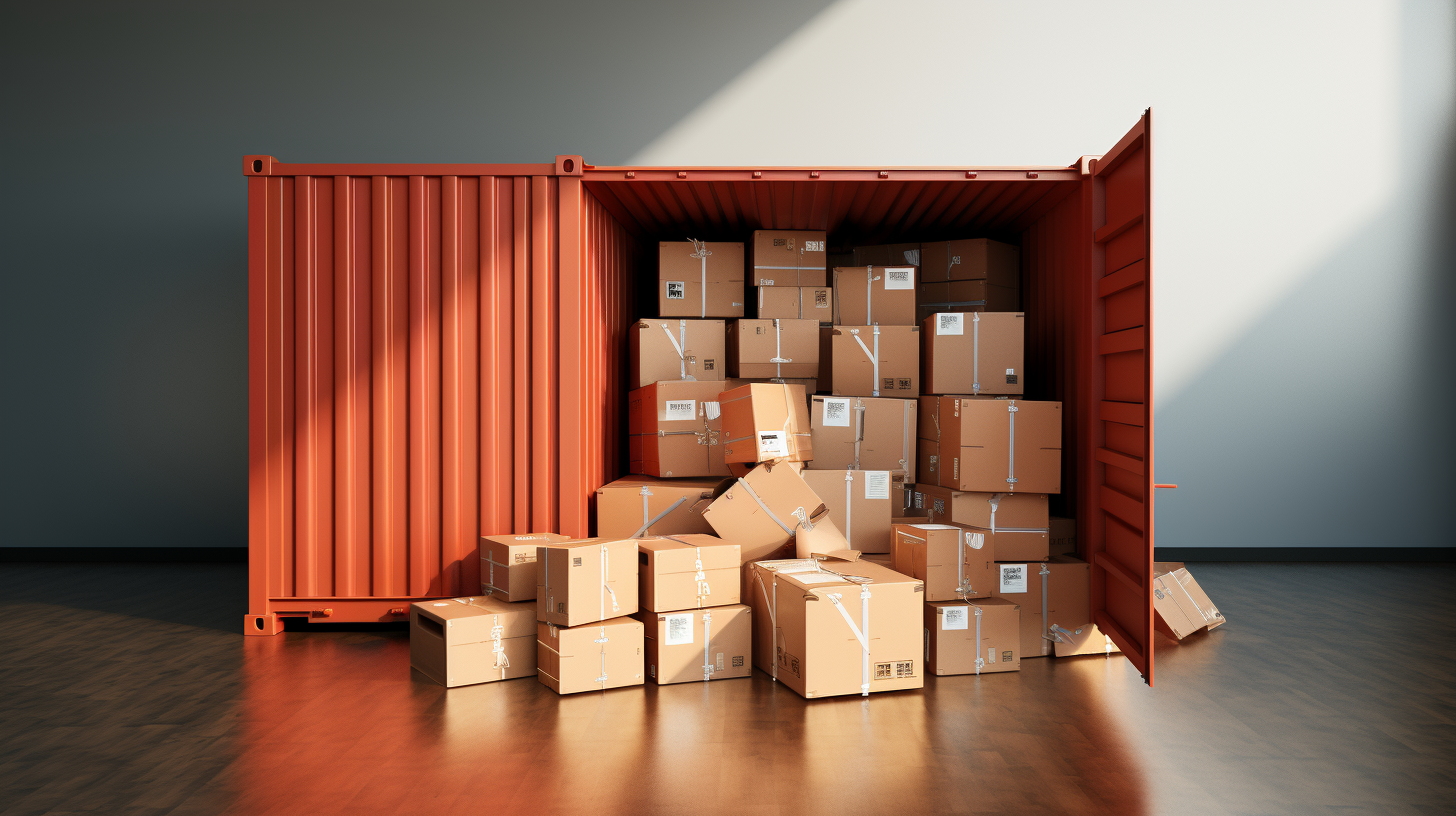
\includegraphics[width = \linewidth]{bin_packing}
		\vskip 0.3cm%
		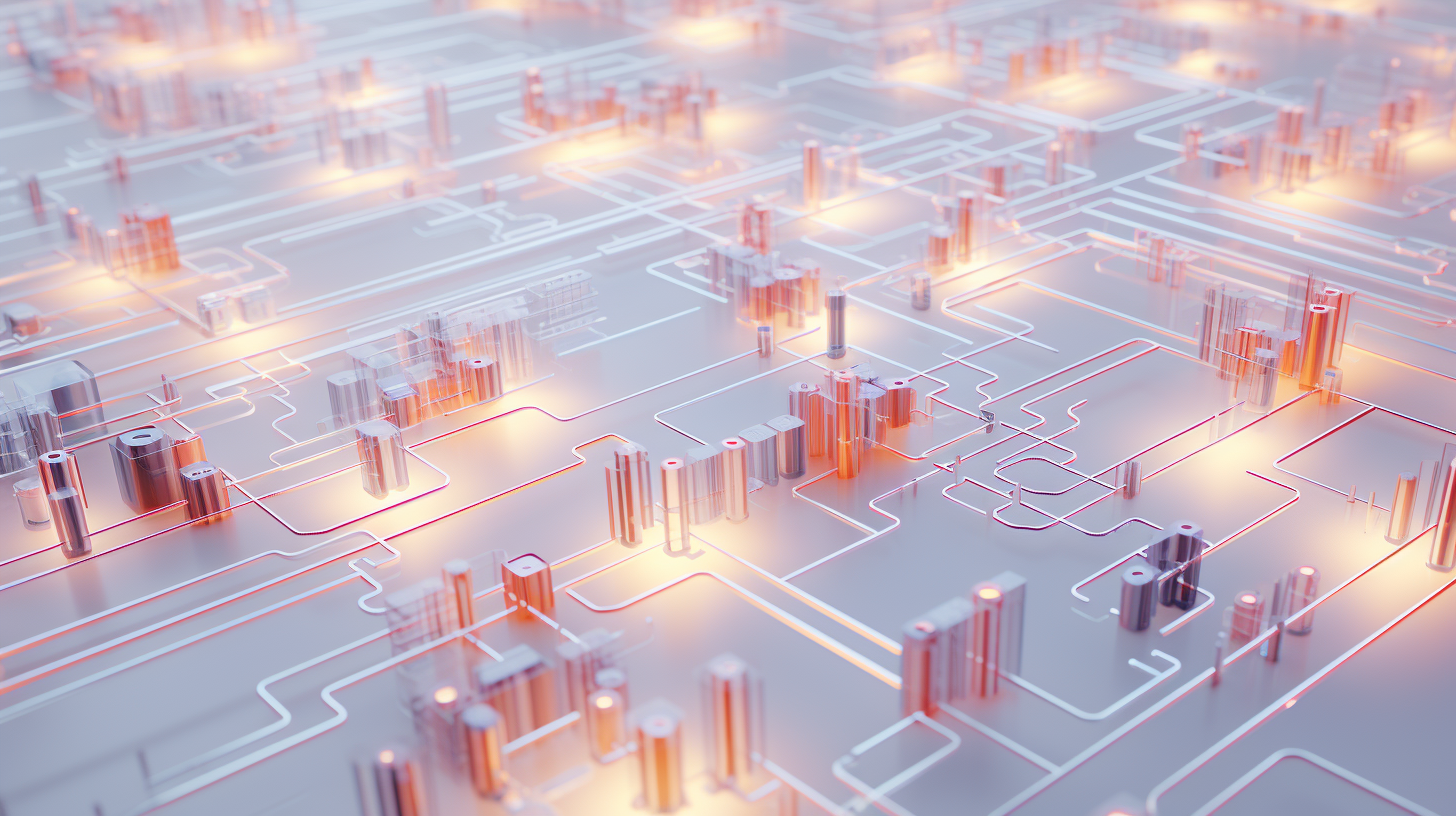
\includegraphics[width = \linewidth]{circuits}
	\end{column}
	\begin{column}{0.43\linewidth}
		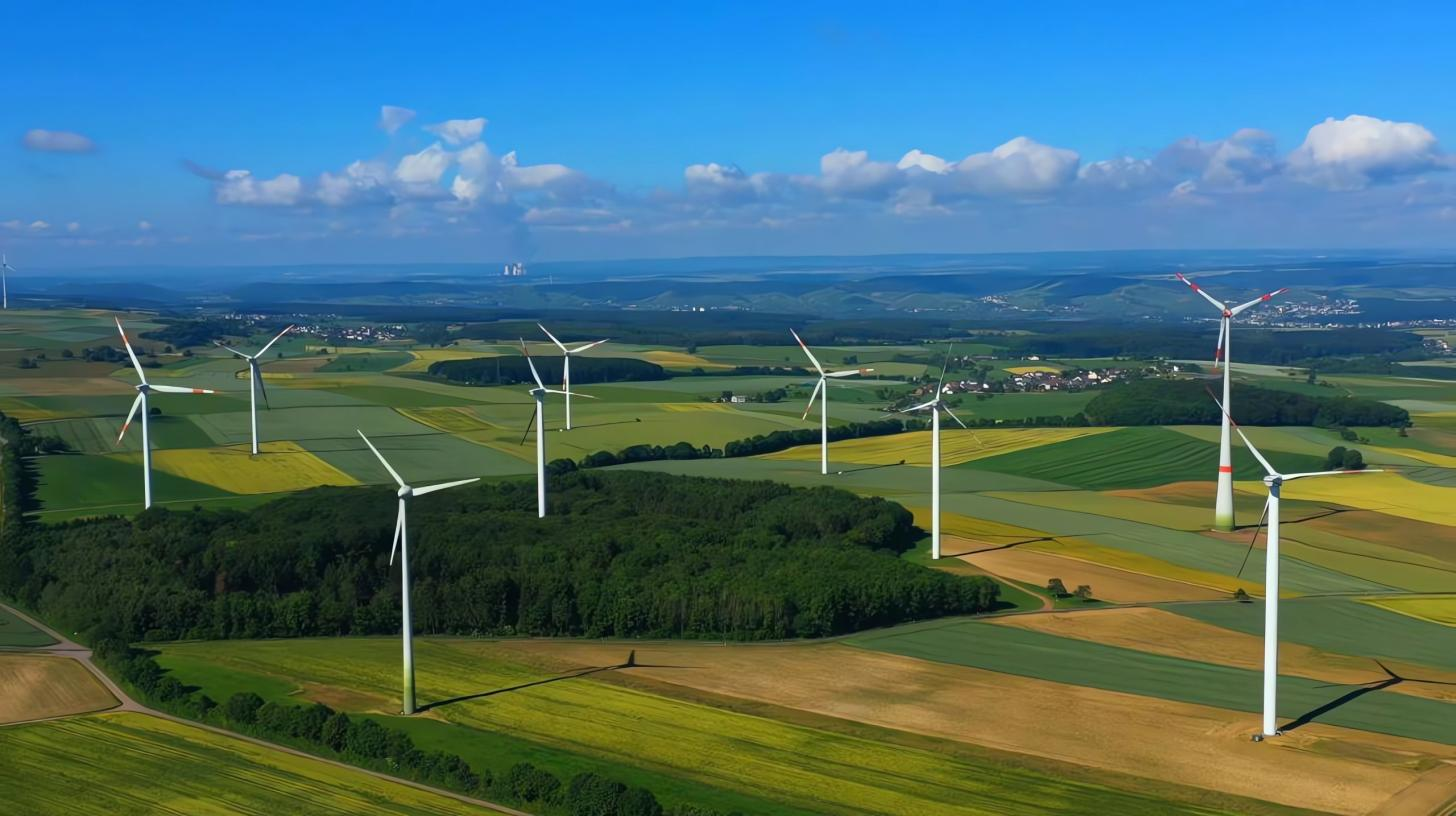
\includegraphics[width = \linewidth]{eolic_park}
		\vskip 0.3cm%
		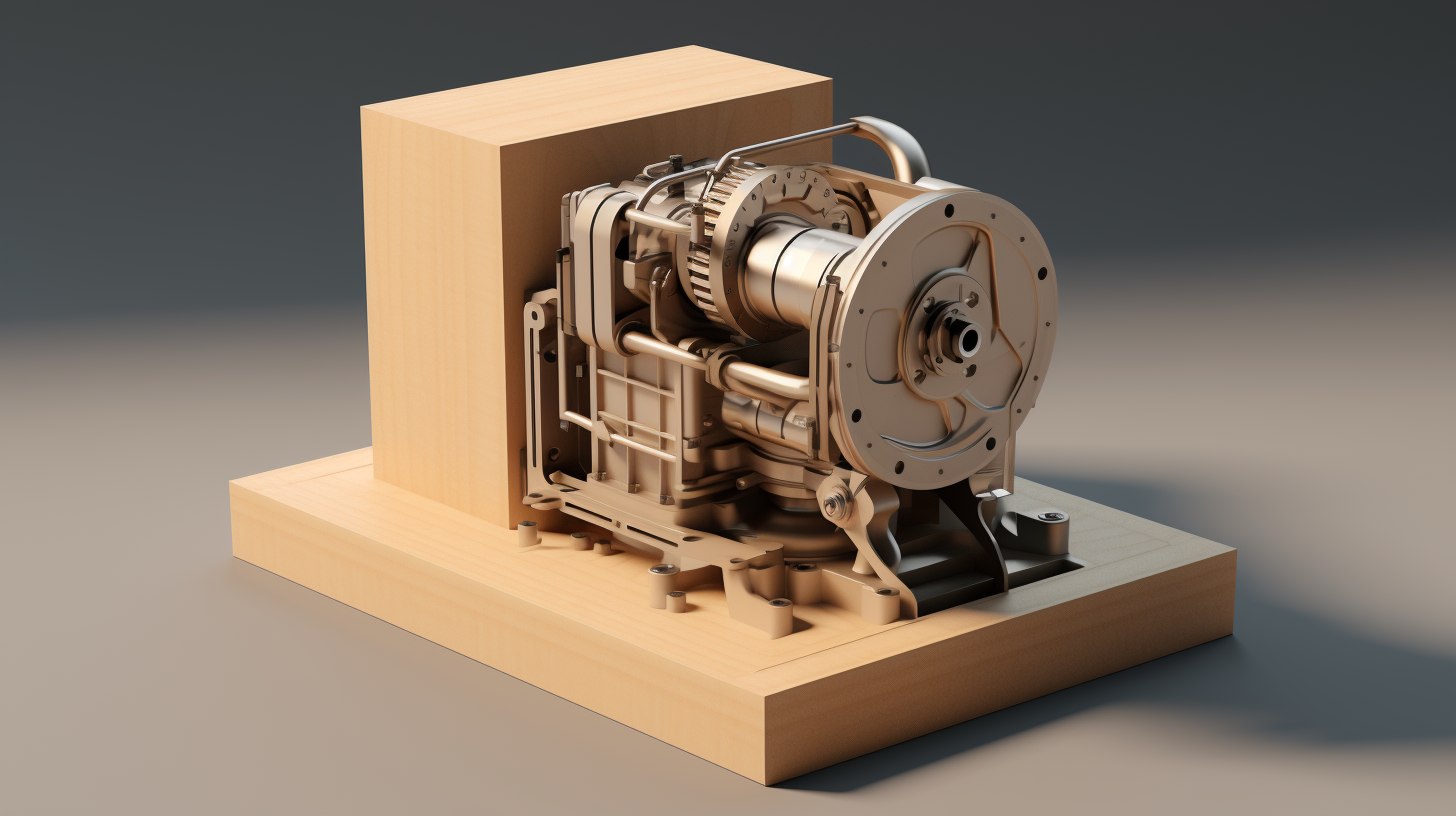
\includegraphics[width = \linewidth]{mechanism}
	\end{column}
	\end{columns}
\end{frame}


\begin{frame}[t]{Características generales del problema}
	\vfill%
	\Wider[-0.2cm]{%
	\begin{columns}[totalwidth = \textwidth]
	\begin{column}[b]{0.48\linewidth}
	\fontsize{14}{16}\selectfont\justifying En el presente trabajo se pretende desarrollar un método para el acomodo de objetos en un espacio delimitado, de tal forma que el costo para acceder (sujetar) a cada uno de estos se minimice.
	\vskip 16.5pt%
	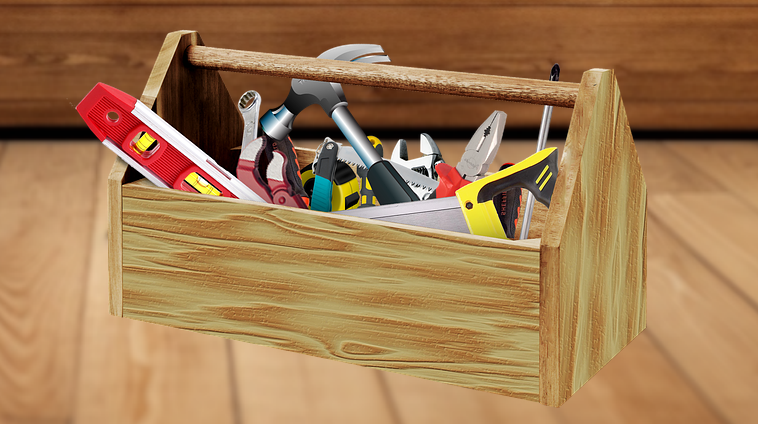
\includegraphics[width = \linewidth]{toolbox}
	\end{column}
	%
	\begin{column}[b]{0.48\linewidth}
		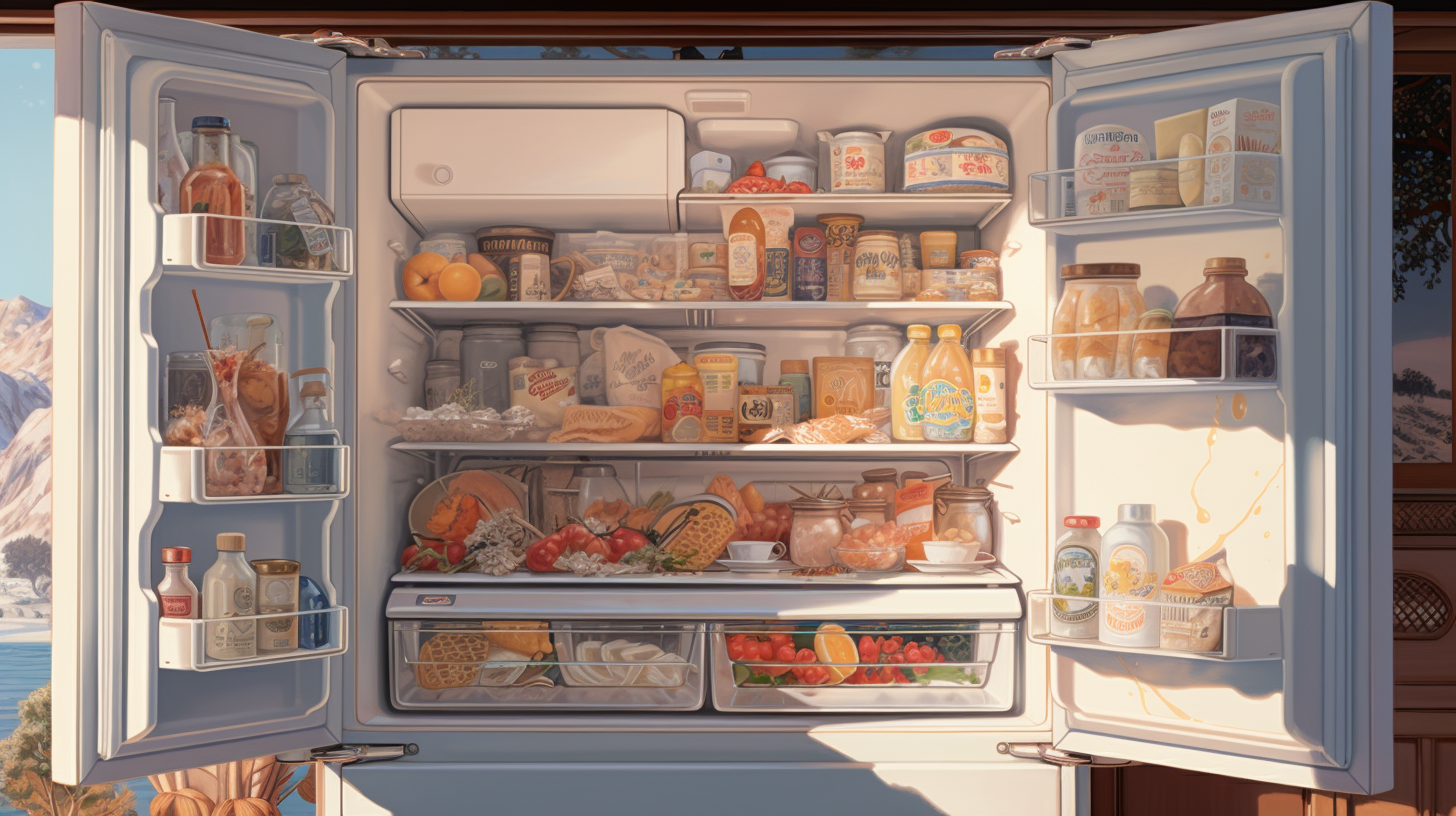
\includegraphics[width = \linewidth]{fridge}
		\vskip 8pt%
		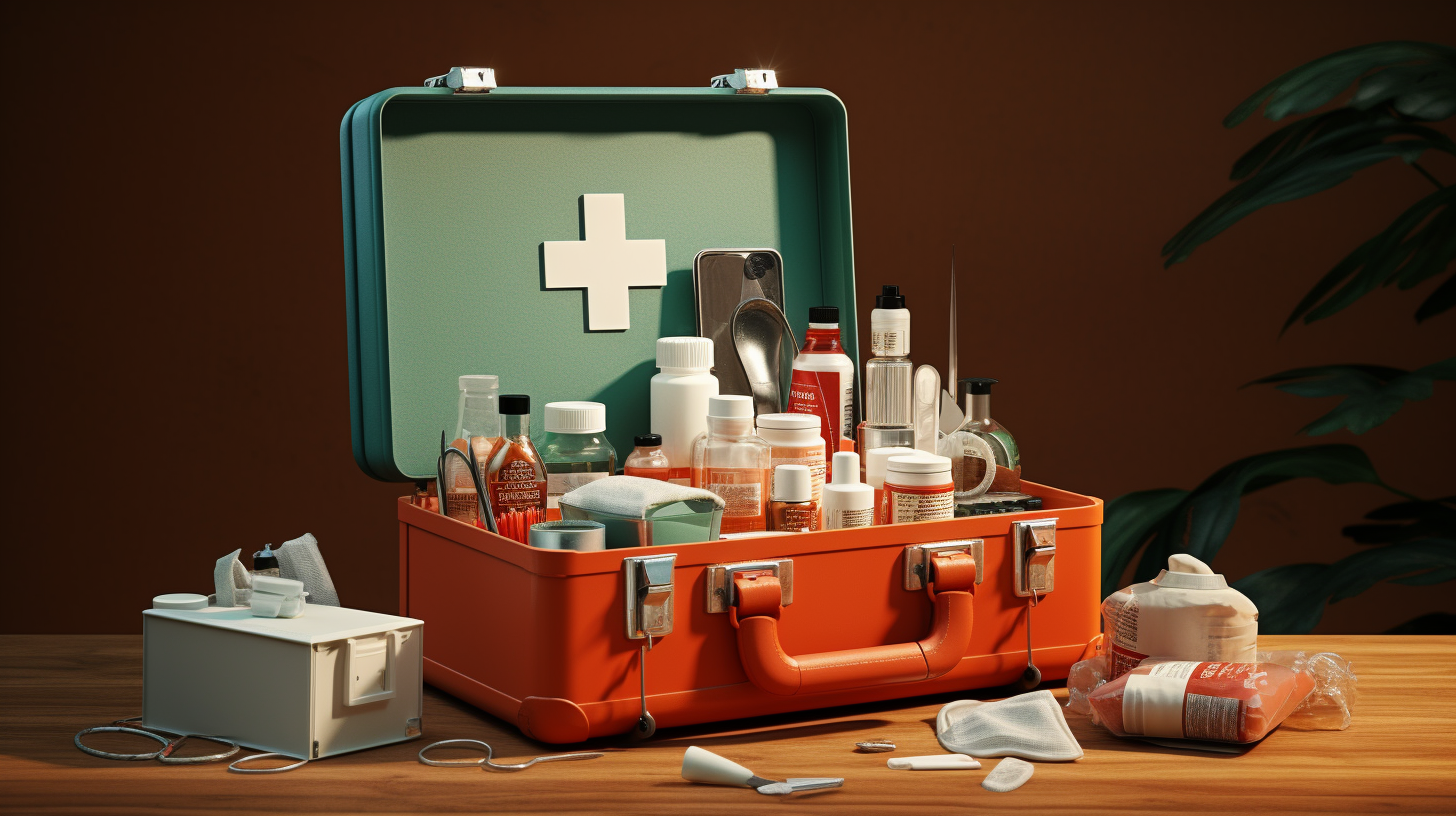
\includegraphics[width = \linewidth]{first_aid_kit}
	\end{column}
	\end{columns}
	}%
\end{frame}


\begin{frame}{Trabajos relacionados}
	\vskip 5pt%
	\fontsize{14}{16}\selectfont%
	\begin{minipage}{\textwidth}
		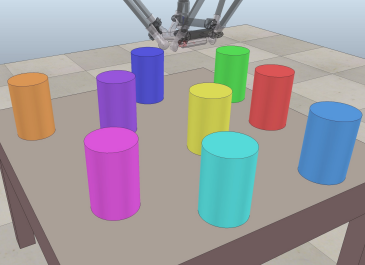
\includegraphics[height = 2.5cm, valign = t]{shuai_han_b} 
		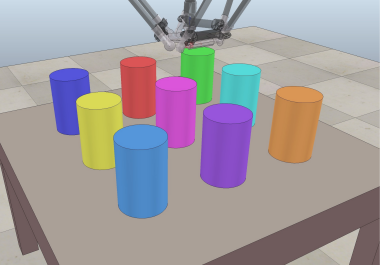
\includegraphics[height = 2.5cm, valign = t]{shuai_han_c} \hfill
		\parbox[t]{0.455\linewidth}{Reordenamiento donde se conoce la configuración final. Imagen tomada de \cite{Han-RSS-17}.}
	\end{minipage}
	\vskip -13pt%
	\begin{minipage}{\textwidth}
		\parbox[t]{0.52\linewidth}{Mover un objeto rodeado de obstáculos a una posición meta. Imagen tomada de \cite{2018arXiv181010654P}.} \hfill 
		\begin{tikzpicture}[>=Triangle, baseline={([yshift={2.8ex}]current bounding box.center)}]
			\node[inner sep = 0pt] at (0, 0) 
				{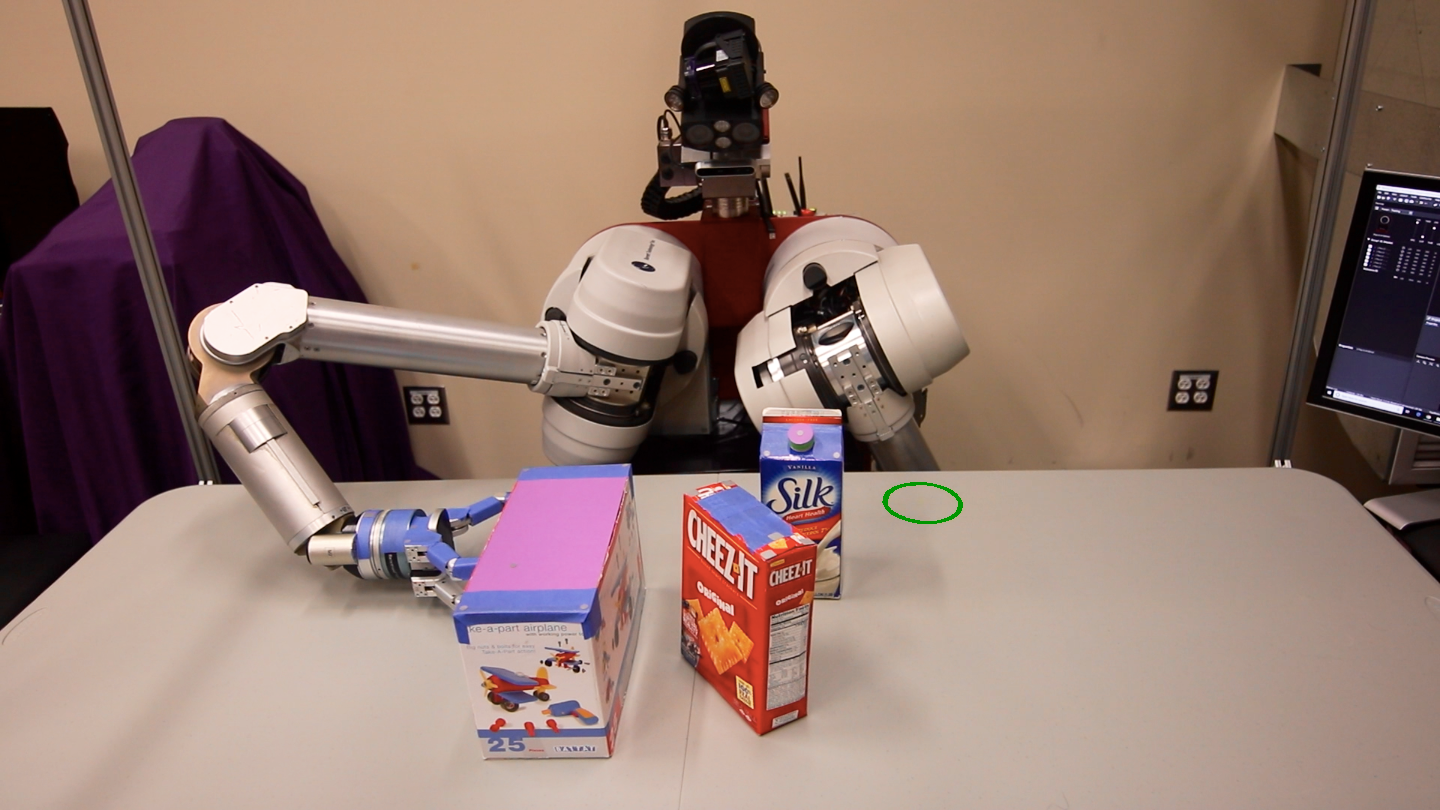
\includegraphics[height = 3.6cm]{lerrel_pinto_a}};
			\node[opacity = 0.4] at (0.95, -0.087) 
				{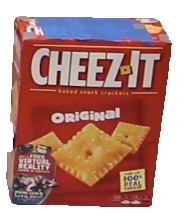
\includegraphics[width = 0.79cm]{lerrel_pinto_b}};
			
			\draw[
				line width = 0.8pt, 
				color = maintextcolor!80, 
				opacity = 0.7, 
				scale = 0.5, 
				shift = {(0.05, -0.1)}
			] 
				
			[arrows = {-Triangle[width = 2pt, length = 2pt]}] 
			(0.6,-1.6) -- (0.9,-2.3) -- (1.6,-2.3)
			node[right = -4pt, maintextcolor, opacity = 1] 
				{\fontsize{5}{5}\selectfont Objetivo};
			
			\draw[
				line width = 0.8pt, 
				color = maintextcolor!80, 
				opacity = 0.7, 
				scale = 0.5, 
				shift = {(0.09, -0.05)}
			]
				
			[arrows = {-Triangle[width = 2pt, length = 2pt]}] 
			(1.7, -0.8) -- (2, -1.5) -- (2.6, -1.5) 
			node[right = -4pt, maintextcolor, opacity = 1] 
				{\fontsize{5}{5}\selectfont Posición meta};
		\end{tikzpicture}
	\end{minipage}
	\vskip -23pt%
	\begin{minipage}{\textwidth}
		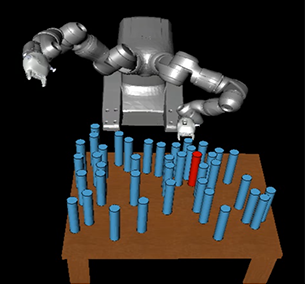
\includegraphics[height = 2.8cm, valign = b]{aliakbar_akbari_b}
		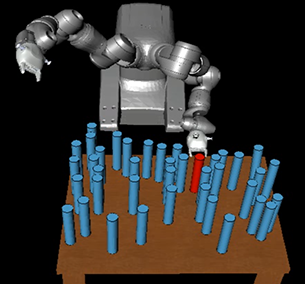
\includegraphics[height = 2.8cm, valign = b]{aliakbar_akbari_f} \hfill 
		\parbox[b]{0.53\linewidth}{Tomar un objeto rodeado de obstáculos en desorden. Imagen tomada de \cite{Akbari2019}.}
	\end{minipage}
\end{frame}


\section{Hipótesis y objetivos}


\frame[noframenumbering, plain]{\tableofcontents[currentsection]}


\begin{frame}{Hipótesis}
	\def\thinkCloud{\raisebox{-1.5pt}{
\includegraphics[width=1em]{think_bubble}}}%
	\begin{itemize}
	\item[\thinkCloud]\itshape Existe una metodología para el acomodo de objetos en un espacio delimitado que minimiza el número promedio de acciones necesarias para acceder (tomar) a cualquiera de ellos.
	\end{itemize}
\end{frame}


\begin{frame}{Objetivo general}
	\begin{itemize}
	\item[\color{verdeOscuro}\raisebox{1pt}{$\blacktriangleright$}] Diseñar un algoritmo para el arreglo de objetos en un espacio delimitado, con la finalidad de que un manipulador sea capaz de acceder a cualquiera de los objetos, realizando un número mínimo de acciones o movimientos.
	\end{itemize}
\end{frame}


\begin{frame}{Objetivos particulares}
	\setbeamerfont{itemize/enumerate body}{size*={14.5pt}{14.5pt}}%
	\vfill%
	\Wider[-1.5cm]{%
		\begin{enumerate}
			\item Analizar la literatura relacionada para comparar los diferentes métodos utilizados en problemas similares.
			\item Seleccionar y adaptar las metodologías útiles para el problema planteado.
			\item Definir las métricas de eficiencia para los algoritmos a implementar.
			\item Proponer un procedimiento adecuado para encontrar arreglos eficientes de objetos.
			\item Evaluar la metodología propuesta.
		\end{enumerate}
	}%
\end{frame}


\section{Marco teórico}


\tcbset{
	skin = enhanced,                                 
	bottom = 2pt, 
	%top = 10pt, 
	left = 3.5pt,
	right = 3.5pt,
	bottomtitle = 1pt, 
	%toptitle = 10pt, 
	lefttitle = 3.5pt, 
	righttitle = 3.5pt
}

\frame[noframenumbering, plain]{\tableofcontents[currentsection]}


\begin{frame}{Espacio de trabajo}
	\begin{columns}
	\column{0.45\textwidth}%
	\vskip -20pt%
	\justifying Se desea que el algoritmo propuesto se aplique a una gran variedad de circunstancias de la vida real, por lo cual se trató de que los fundamentos de este fueran lo más generales posible.
	\column{0.55\textwidth}%
	\vspace{-8pt}%
	\begin{block}{Definición}
		Sea $E$ un espacio discreto (malla) de $n\times m$ localidades o celdas, cada una representada por $e_{ij}$. 
	\end{block}
	\vskip -2pt%
	\centering
	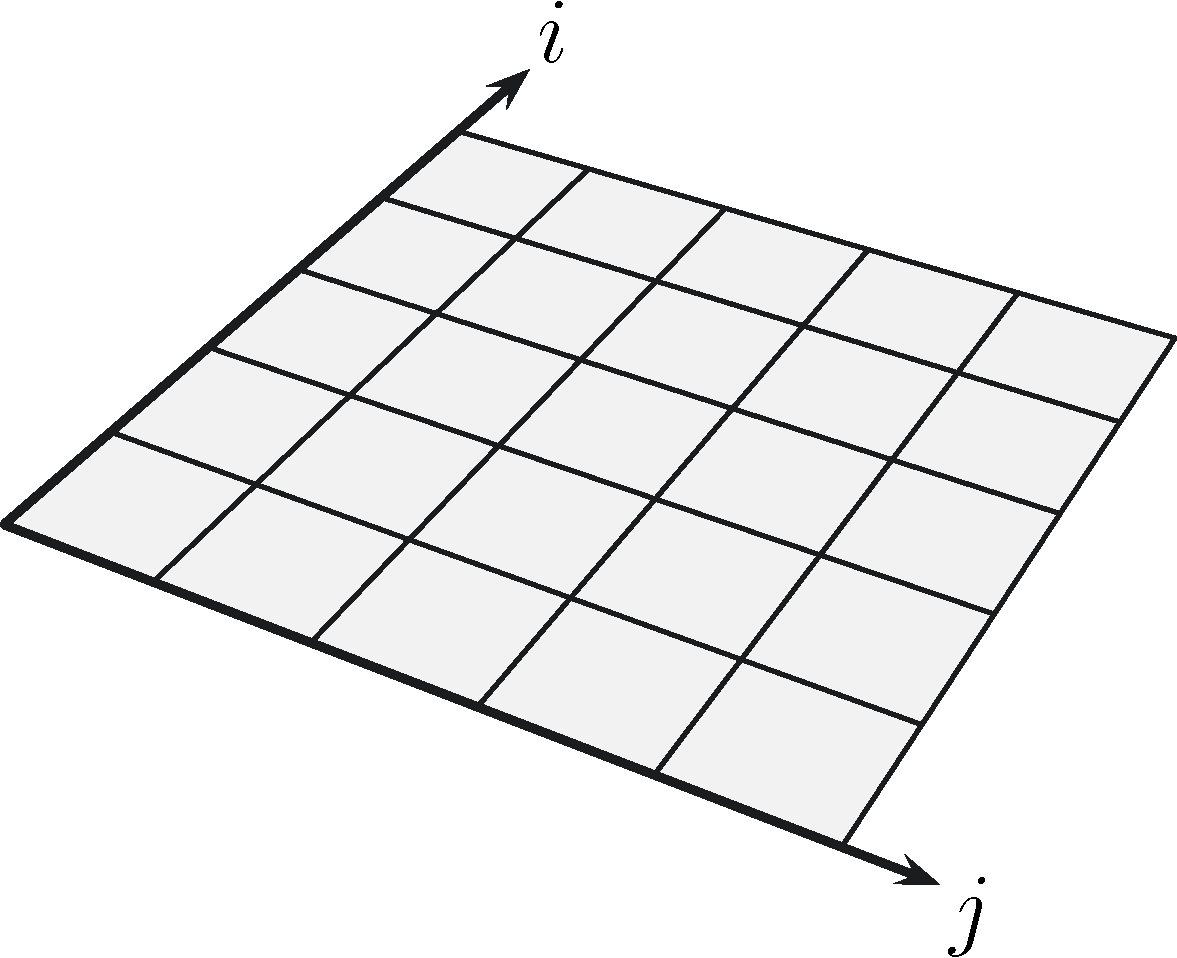
\includegraphics[width = 0.74\textwidth]{ejes_malla}
	\end{columns}
\end{frame}


\begin{frame}{Conjunto de objetos}
	Se desea colocar en $E$ un grupo de objetos.
	\begin{block}{Definición}
		Sea $O = \{o_1, o_2, \cdots\hspace{-1pt}, o_N\}$ el conjunto de objetos disponibles para colocar en las celdas de $E$, donde $N$ es el número total de objetos y $N \leq nm$.
	\end{block}
	\vfill
	\centering
	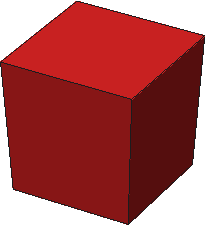
\includegraphics[width=2cm]{cubo}
	\hskip 1.5cm%
	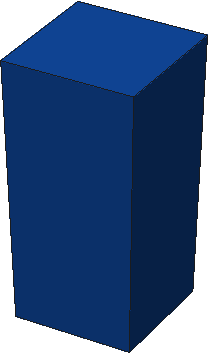
\includegraphics[width=2cm]{prisma}
\end{frame}


\begin{frame}{Atributos de los objetos}
	\setlength{\abovedisplayskip}{10pt}
	\vspace{-8pt}%
	\begin{block}{Definición}
		Sea $A = \{a_1, a_2, \cdots\hspace{-1pt}, a_{N_A}\}$ el conjunto de atributos que puede tener un objeto, por ejemplo el tamaño, color, forma, etc.
	\end{block}
	%
	\begin{block}{Definición}
		Sea $A_k = \{a_{k, 1}, a_{k, 2}, \cdots\hspace{-1pt}, a_{k, N_A}\}$ el conjunto de atributos asociado a un determinado objeto $o_k$.
	\end{block}
	%\vskip 0.15cm%
	Es decir, si por ejemplo, $o_1 \equiv 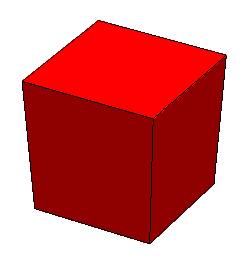
\includegraphics[width=15pt, valign=c]{Cubo}$ y $o_2 \equiv 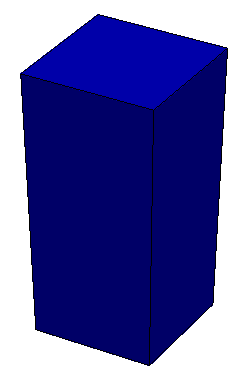
\includegraphics[width=15pt, margin*={0.0cm, -0.2cm, 0.0cm, 0.0cm}]{Prisma}$, entonces:
	%
	\begin{align*}
		A = \{\textsl{altura}, \textsl{color}, \ldots\}\qquad &
		\begin{aligned}
			A_1 &= \{\text{10cm}, \text{rojo}, \ldots\} \\
			A_2 &= \{\text{20cm}, \text{azul}, \ldots\}
		\end{aligned}
	\end{align*}
\end{frame}


\begin{frame}{Clases de objetos}
	\setlength{\abovedisplayskip}{0.75cm}
	\addtobeamertemplate{block begin}{\vskip 0.3cm}{}
	\addtobeamertemplate{block end}{}{\vskip 0.4cm}
	\begin{block}{Definición}
		Se define $C = \{C_1, C_2, \cdots\hspace{-1pt}, C_{N_C}\}$ como el conjunto de clases distintas de objetos, donde cada clase representa un $A_k$ distinto, siendo $N_C$ el número total de clases o $A_k$'s diferentes.
	\end{block}
	%
	Entonces, si $o_1 \equiv 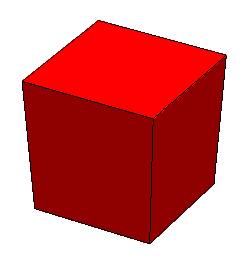
\includegraphics[width=15pt, valign=c]{Cubo}$ y $o_2 \equiv 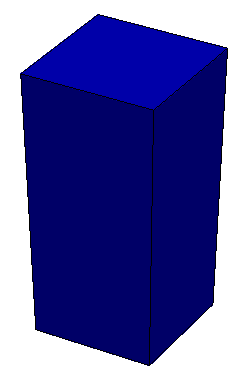
\includegraphics[width=15pt, margin*={0.0cm, -0.2cm, 0.0cm, 0.0cm}]{Prisma}$:
	%
	\begin{align*}
		&\text{\f{clase}($o_1$)} = C_1 \equiv \text{atributos cubo} \\[5pt]
		&\text{\f{clase}($o_2$)} = C_2 \equiv \text{atributos prisma}
	\end{align*}
\end{frame}


\begin{frame}{Vecindad}
	\vspace{-6pt}%
	\begin{block}{Definición}
		Se define una vecindad $V_{ij} = \{v_1, v_2, \cdots\hspace{-1pt}, v_{N_V}\}$, como un conjunto de celdas, las cuales se consideran localidades vecinas a la localidad $e_{ij}$.
	\end{block}
	\vfill
	\centering
	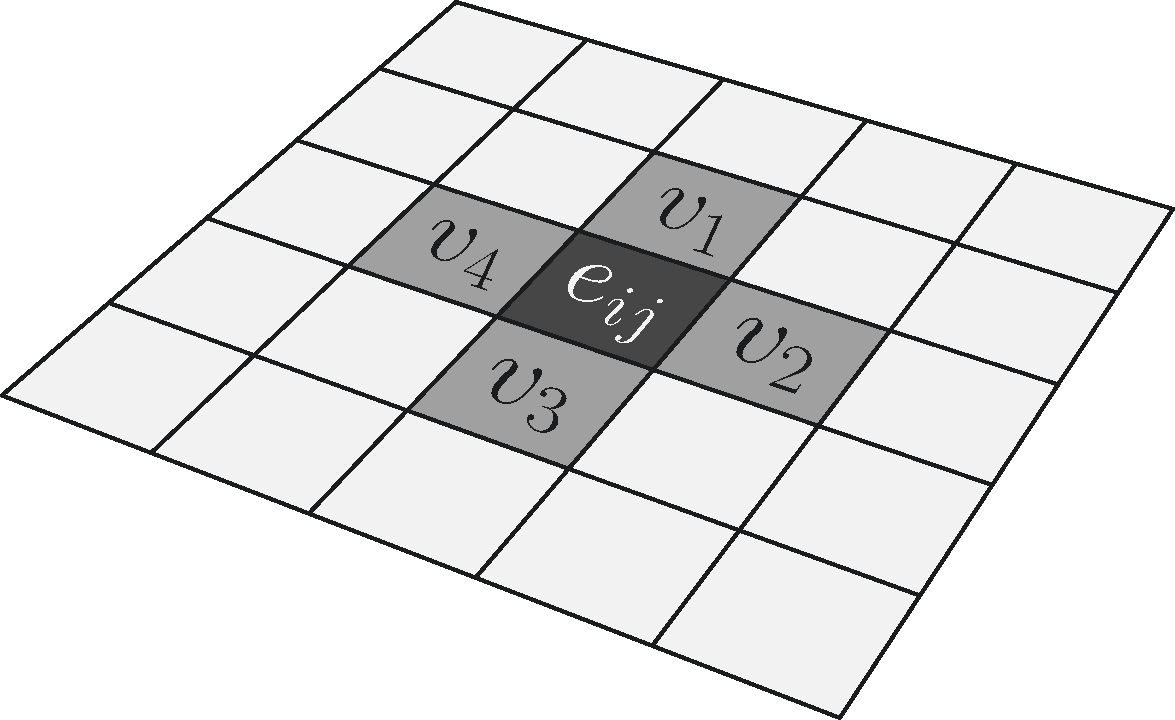
\includegraphics[width=7cm]{vecindad}
\end{frame}


\begin{frame}{Formas de sujeción}
	\vspace{-1pt}%
	\begin{block}{Definición}
		Sea $S_K = \{s_{K, 1}, s_{K, 2}, \cdots\hspace{-1pt}, s_{K, N_S}\}$ el conjunto de formas de sujeción asociado a una clase $C_K$.
	\end{block}
	\vskip 3pt%
	Por ejemplo, si $S_1 = S_2 = \{H, V\}$:
	\vskip 3pt%
	\begin{figure}[H]
		\captionsetup[subfigure]{width=1.05\linewidth, skip=1pt}%
		\begin{subfigure}{4.5cm}
			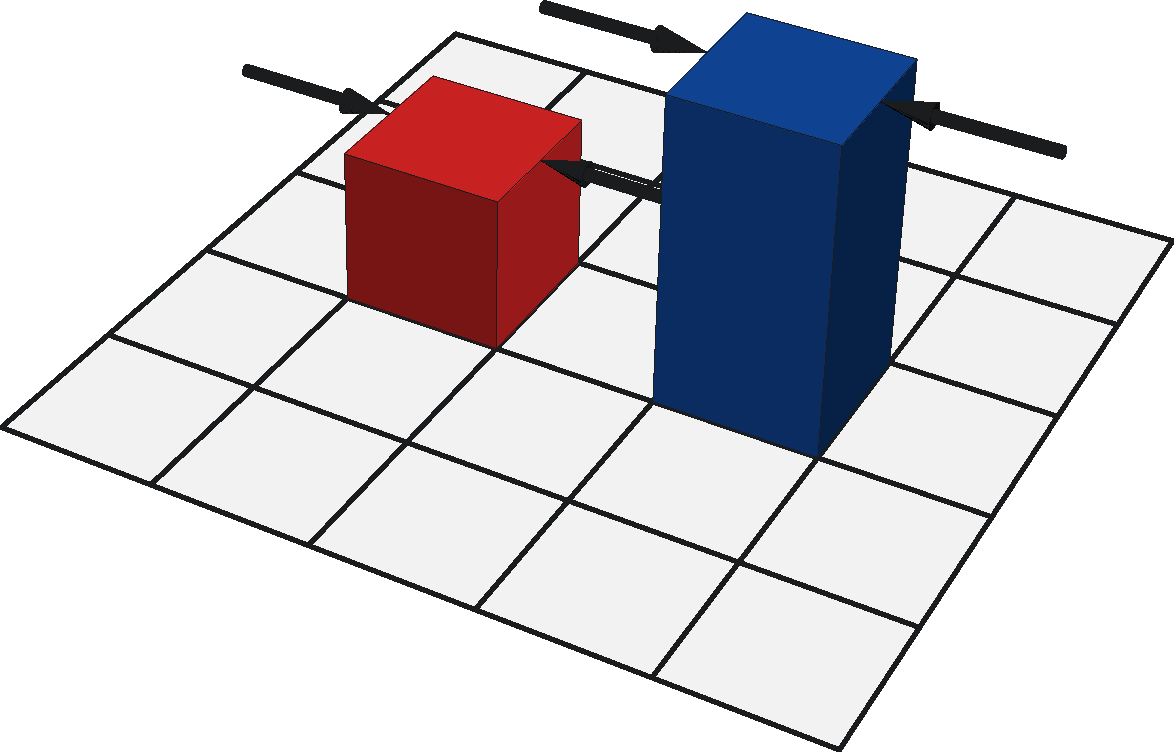
\includegraphics[width=\linewidth]{agarre_horizontal}%
			\caption{Forma de sujeción $H$.}%
		\end{subfigure}%
		\hspace{1.75cm}%
		\begin{subfigure}{4.5cm}
			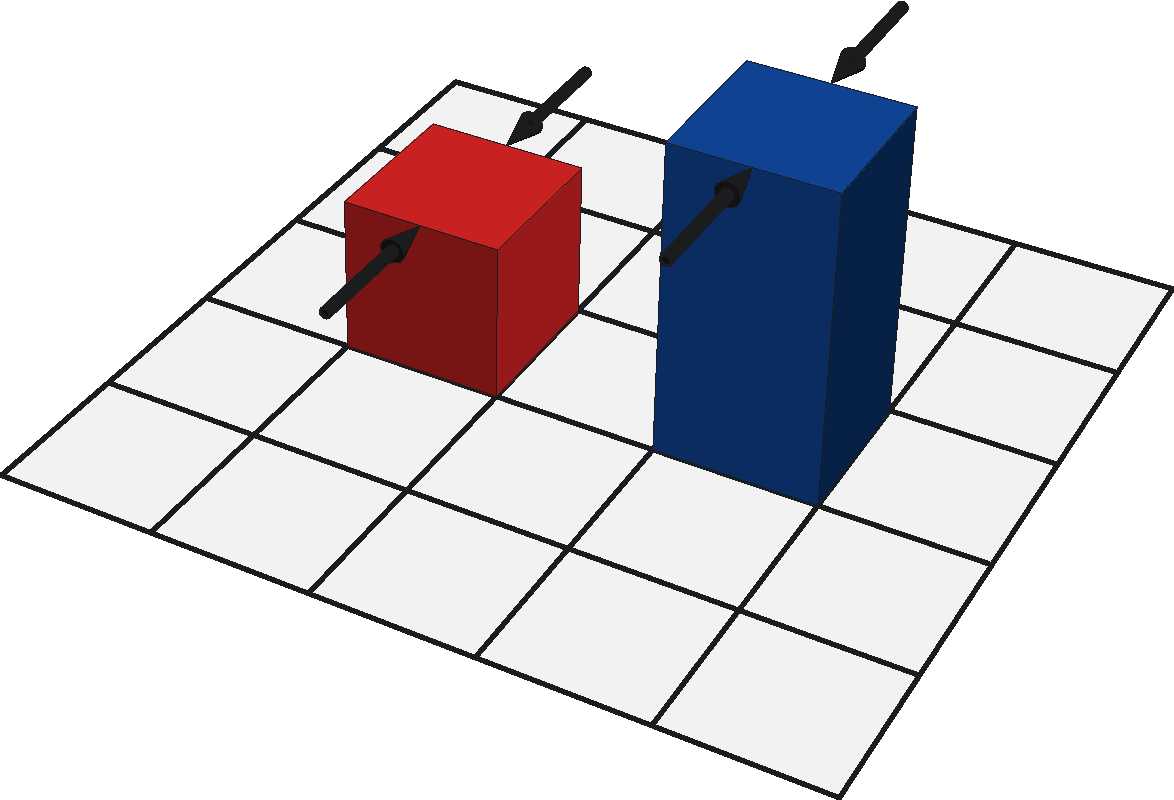
\includegraphics[width=\linewidth]{agarre_vertical}%
			\caption{Forma de sujeción $V$.}%
		\end{subfigure}
	\end{figure}
\end{frame}


\begin{frame}{Restricciones de sujeción}
	\captionsetup[figure]{
		labelformat = empty, 
		format = hang, 
		justification = justified, 
		belowskip = 4pt, 
		aboveskip = -1pt
	}%
	\begin{figure}[H]
	\def\figswidth{0.25\textwidth}%
	\def\figshsep{1cm}%
		\caption{Ejemplos de cómo se pueden restringir las formas de sujeción en función de la vecindad de un objeto.}%
    	\begin{subfigure}{\figswidth}
			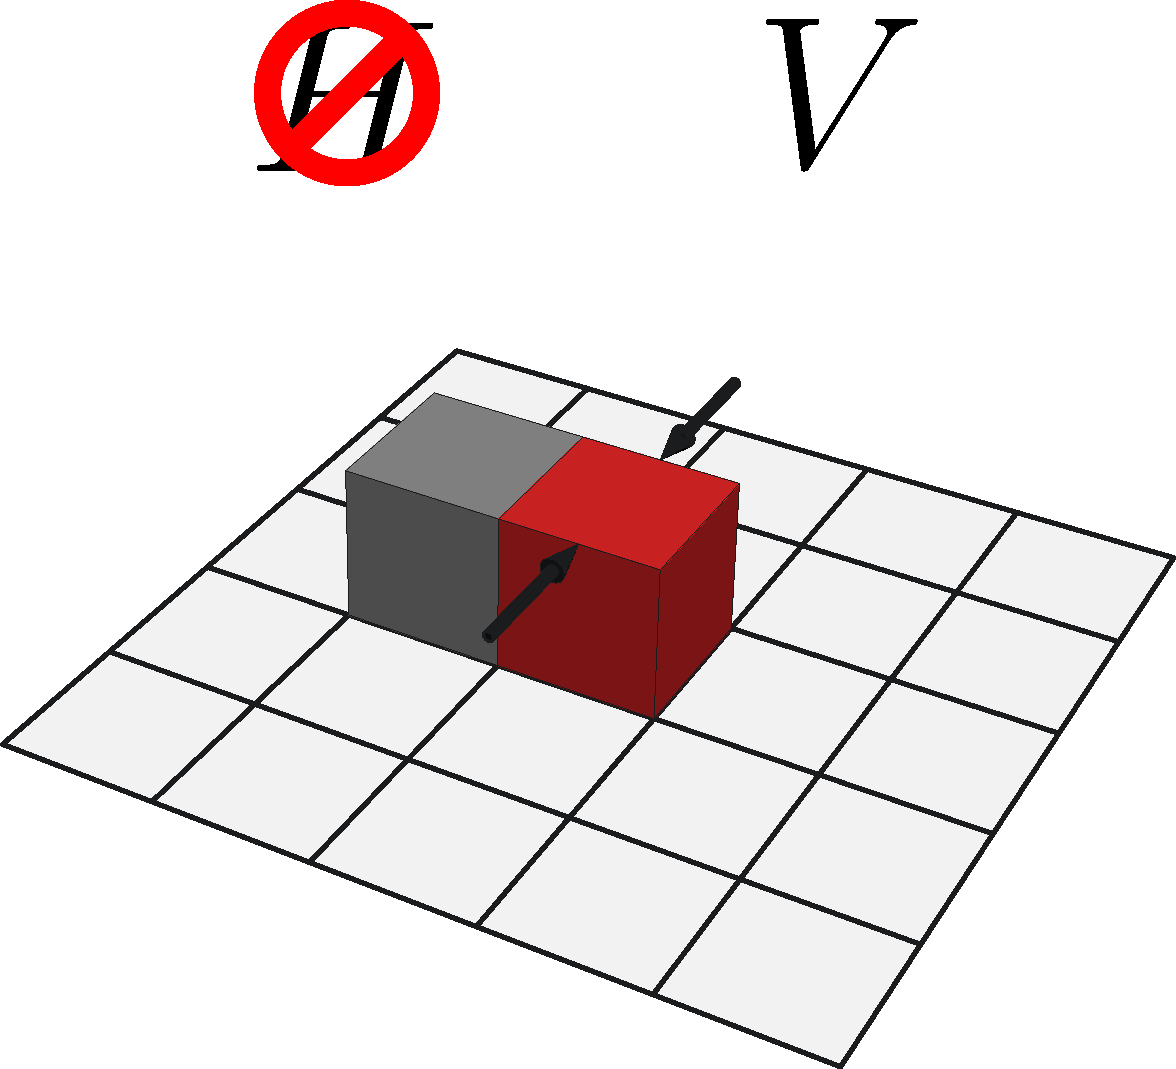
\includegraphics[width=\textwidth]{restriccion_H_cubo}
			%\caption{Restricción de $H$ en un cubo.}
    	\end{subfigure}
    	\hskip \figshsep%
    	\begin{subfigure}{\figswidth}
       		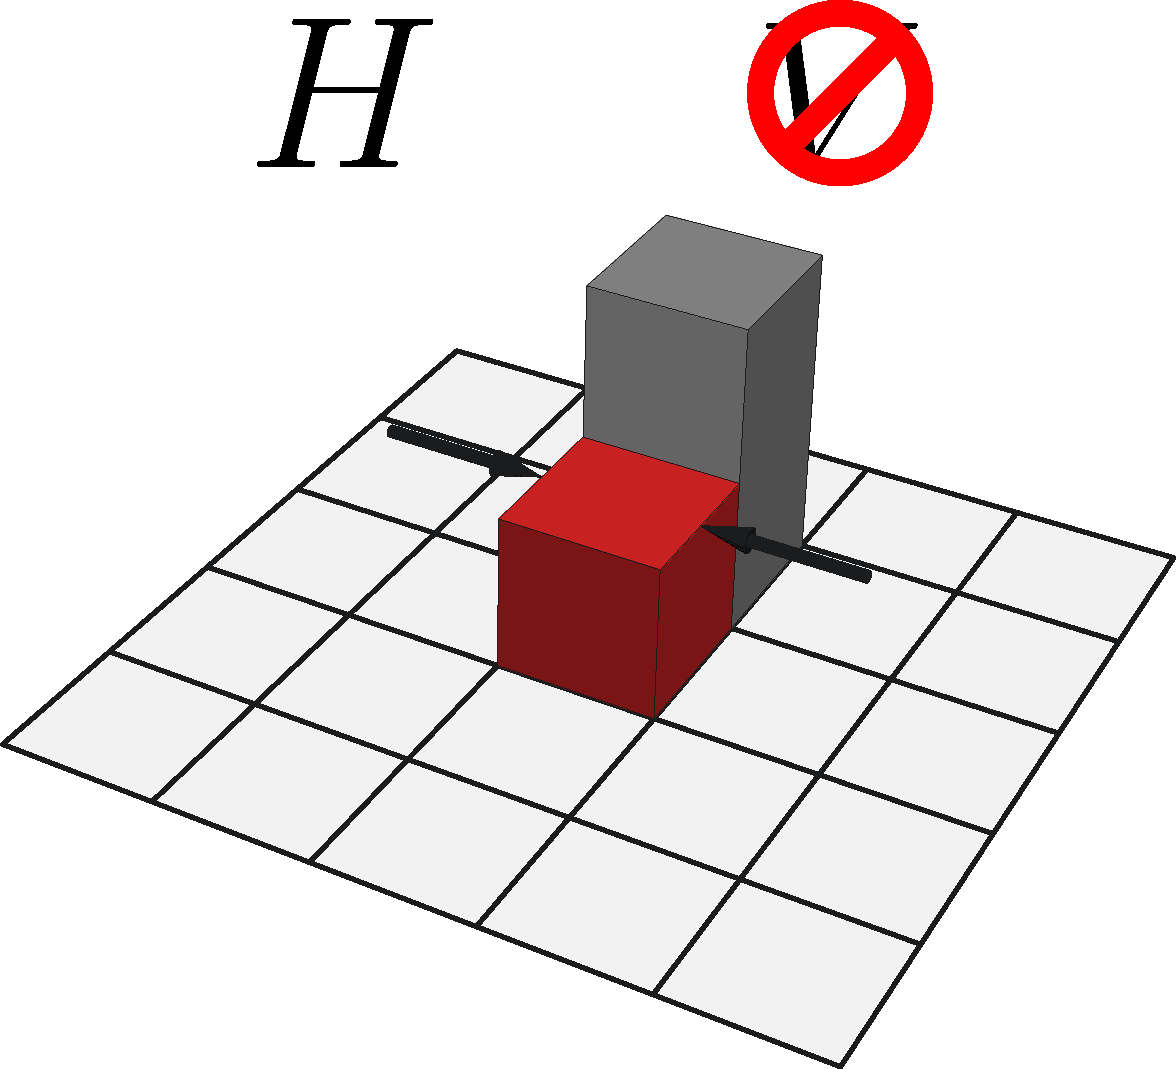
\includegraphics[width=\textwidth]{restriccion_V_cubo}
       		%\caption{Restricción de $V$ en un cubo.}
    	\end{subfigure}
    	\hskip \figshsep%
    	\begin{subfigure}{\figswidth}
       		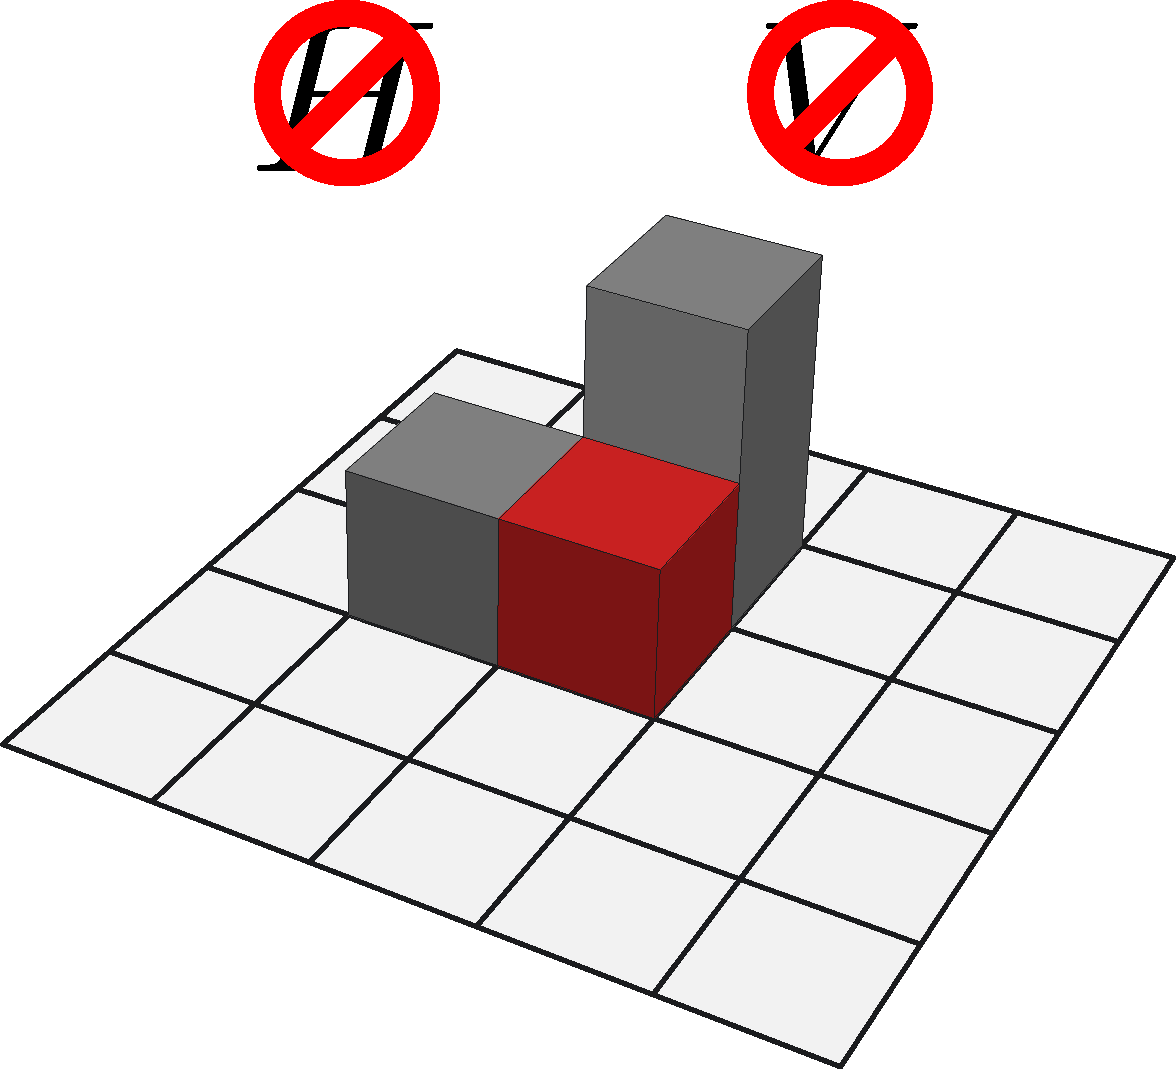
\includegraphics[width=\textwidth]{restriccion_HV_cubo}
       		%\caption{Restricción de $H$ y $V$ en un cubo.}
    	\end{subfigure}%
    	\vskip 5pt%
    	\begin{subfigure}{\figswidth} 
			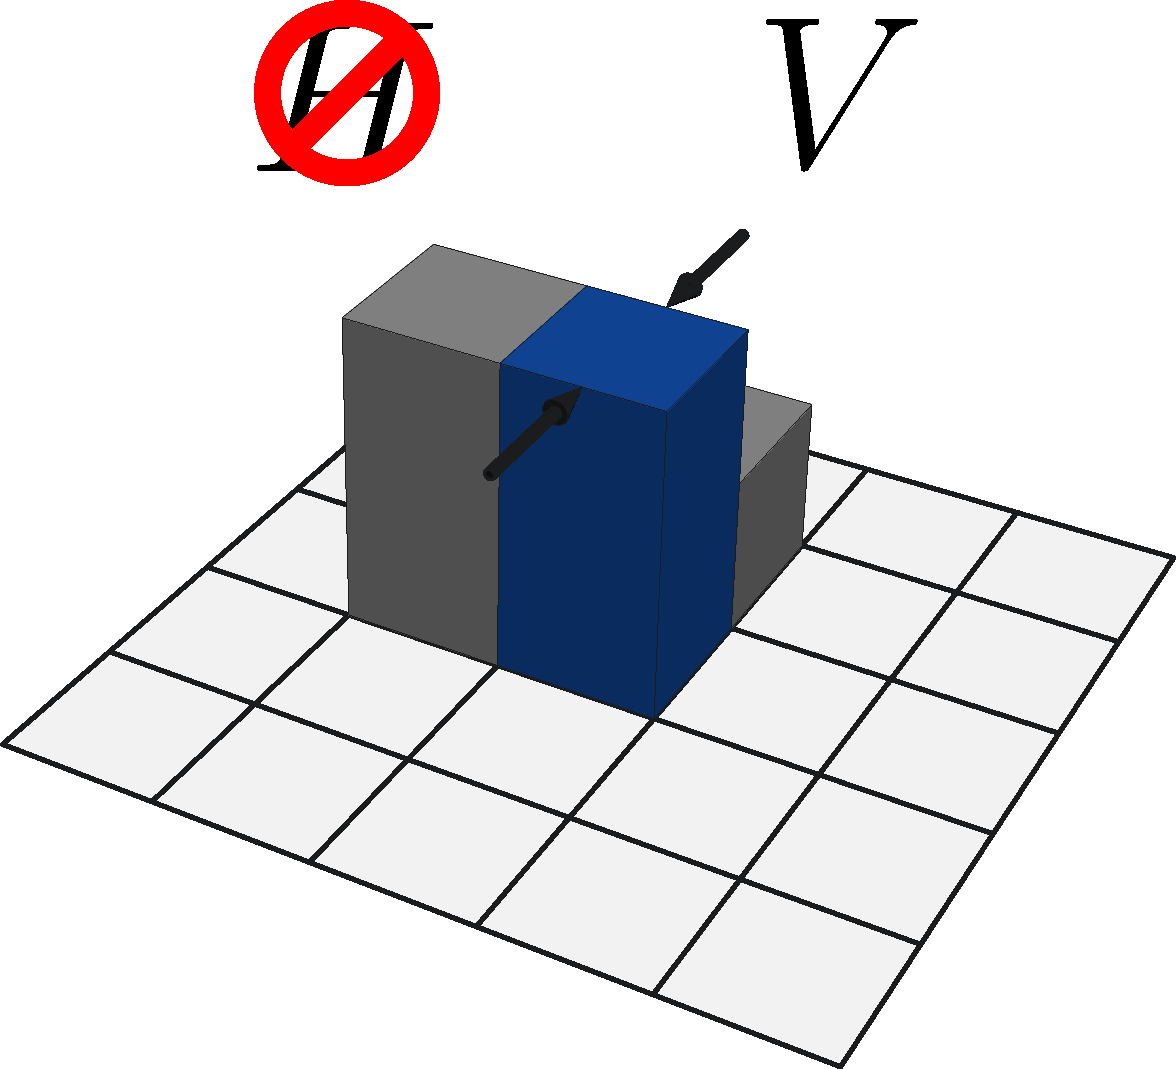
\includegraphics[width=\textwidth]{restriccion_H_prisma}
			%\caption{Restricción de $H$ en un prisma.}
		\end{subfigure}
		\hskip \figshsep%
    	\begin{subfigure}{\figswidth}
       		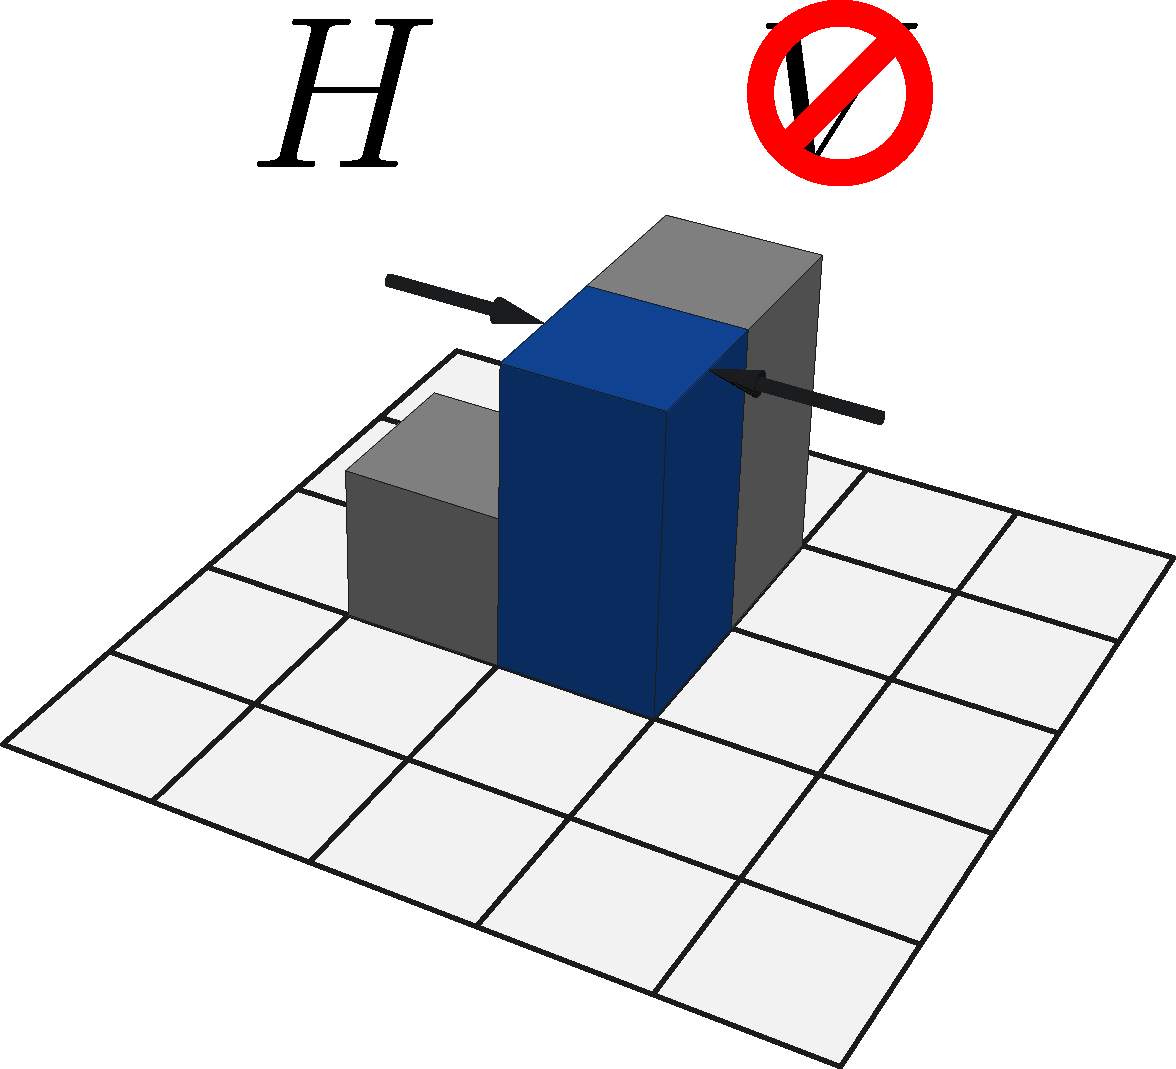
\includegraphics[width=\textwidth]{restriccion_V_prisma}
       		%\caption{Restricción de $V$ en un prisma.}
    	\end{subfigure}
    	\hskip \figshsep%
    	\begin{subfigure}{\figswidth}
       		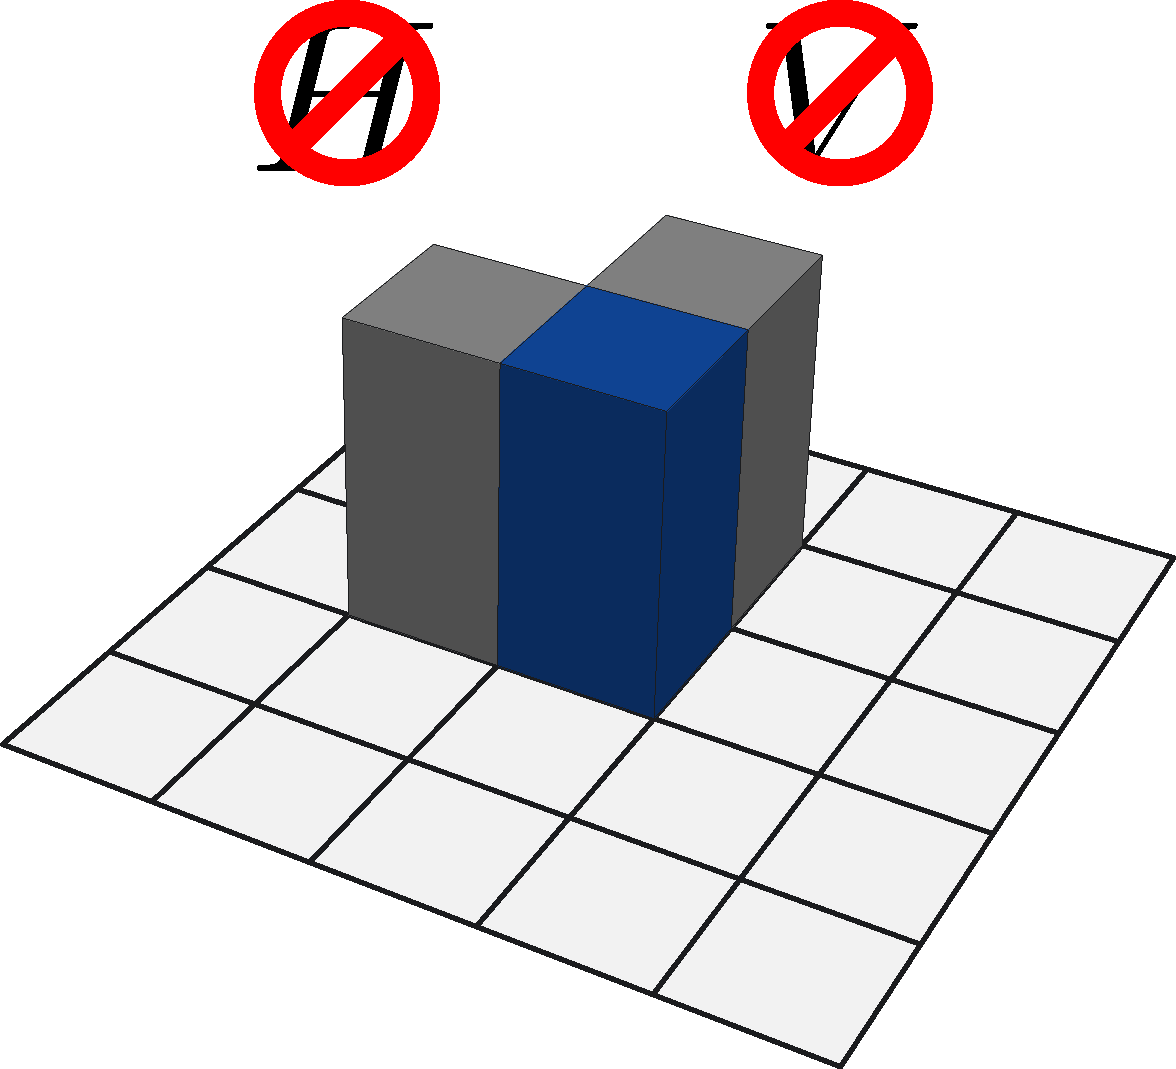
\includegraphics[width=\textwidth]{restriccion_HV_prisma}
       		%\caption{Restricción de $H$ y $V$ en un prisma.}
    	\end{subfigure}%
    \end{figure}
\end{frame}


\begin{frame}{Costos de acceso a los objetos}
	\fontsize{14}{16}\selectfont
	\vspace{-5.5pt}%
	\begin{block}{Definición}
		Sea $t_{ij}$ la variable discreta que cuantifica el número de acciones necesarias para tomar el objeto en $e_{ij}$, lo cual se denomina como el costo de tomar un objeto.
	\end{block}
	%
	Así, $t_{ij} - 1$ corresponderá al número de objetos-obstáculo que hay que retirar antes de tomar un objeto de interés.
	\vspace{-3pt}%
	%
	\begin{block}{Definición}
		\setlength{\abovedisplayskip}{10pt}%
		Asimismo, se define el costo global $T$ de un acomodo de objetos como la suma de los costos individuales $t_{ij}$:
		\begin{equation*}
			T = \sum_{i,\,j}\ t_{ij}
		\end{equation*}
	\end{block}
\end{frame}


\section{Metodología propuesta}


\tcbset{                              
	bottom = 0pt, 
	top = 0pt, 
	left = 0pt,
	right = 0pt,
	bottomtitle = 0.5pt, 
	toptitle = 1.5pt, 
	lefttitle = 2pt, 
	righttitle = 0pt
}


\setbeamerfont{block title}{shape = \normalfont}


\frame[noframenumbering, plain]{\tableofcontents[currentsection]}


\begin{frame}{Funciones de puntuación}
	\vskip -12pt%
	\Wider[0.6cm]{%
	\begin{columns}[totalwidth = \textwidth]
	\begin{column}{0.58\textwidth}
	\begin{block}{Función: \f{puntuacionPar}($e_{i_1 j_1}$, $e_{i_2 j_2}$)}
	\footnotesize%
	\makeatletter%
	\setboolean{algocf@hanginginout}{false}%
	\makeatother%
	\begin{function}[H]
	\addtolength{\hsize}{\algomargin}%
	\HalfQuarterBlankLine
	\Data{\setstretch{0.8}Celdas de los elementos vecinos.}
	\HalfBlankLine
	\Result{Puntuación del par de vecinos.}
	\HalfBlankLine
	\Definitions{\justifying $C_{ij}$: clase del elemento en $e_{ij}$.\newline $C_0$: celda vacía.}
	\HalfBlankLine
	\nonl\nlset{1}%
	\SetAlgoNoEnd%
	\Function{$\f{puntuacionPar}\:\!(e_{i_1 j_1}, e_{i_2 j_2})$}{
		\HalfBlankLine
		\SetAlgoShortEnd%
		\Switch{$C_{i_1 j_1}$, $C_{i_2 j_2}$}{%
			\HalfBlankLine
			\lCase{$C_1$, $C_0$}{\Return 3}
			\lCase{$C_1$, $C_2$}{\Return 1}
			\lCase{$C_2$, $C_1$}{\Return 2}
			\lCase{$C_2$, $C_0$}{\Return 1}
			\lCase{$C_0$, $C_1$}{\Return 2}
			\lCase{$C_0$, $C_2$}{\Return 1}
			\lCase{$C_{k_C}$, $C_{k_C}$}{\Return 0}
			\vskip -1pt%
		}
		\vskip -1pt%
	}\nonl\nlset{11}\textbf{end}
	%\caption{puntuacionPar($e_{i_1,j_1}$, $e_{i_2,j_2}$). Función para obtener la puntuación de un par de elementos vecinos.}
	\end{function}
	\end{block}
	\end{column}
	%
	\begin{column}{0.38\textwidth}
		\justifying%
		\fontsize{15}{17}\selectfont Función para obtener la puntuación de un par de elementos vecinos en la malla.
		\vskip 20pt%
		\centering%
		
\includegraphics[width = 0.85\linewidth]{puntuacion_par}
	\end{column}
	\end{columns}
	}
\end{frame}


\begin{frame}{Funciones de puntuación}
	\vskip -11pt%
	\Wider[0.6cm]{%
	\begin{columns}[totalwidth=\textwidth]
	\begin{column}{0.58\textwidth}
	\begin{block}{Función: \f{puntuacionElemento}($e_{ij}$)}
	\footnotesize%
	\begin{function}[H]
	\addtolength{\hsize}{\algomargin}%
	\BlankLine
	\Data{Celda del elemento a puntuar $e_{ij}$.}
	\QuarterBlankLine
	\Result{Puntuación $p$ del elemento.}
	\BlankLine
	\nonl\nlset{1}%
	\SetAlgoNoEnd%
	\Function{$\f{puntuacionElemento}(e_{ij})$}{
		\HalfQuarterBlankLine
		\SetAlgoShortEnd%
		$p_H = \f{puntPar}\:\!(e_{ij},\: V_{i, j, 2}) +\, \f{puntPar}\:\!(e_{ij},\: V_{i, j, 4})$\;
		\QuarterBlankLine
		$\mathrlap{p_V}\hphantom{p_H} = \f{puntPar}\:\!(e_{ij},\: V_{i, j, 1}) +\, \f{puntPar}\:\!(e_{ij},\: V_{i, j, 3})$\;
		\BlankLine
		$p = p_H + p_V$\;
		\OneHalfBlankLine
		\If{$C_{ij} \neq C_0$}{
			\BlankLine
			\lIf{$\mathrlap{\f{sujetable}(e_{ij})}\hphantom{\f{imposible}(e_{ij})}$}{$p\ \!\!= \max(p_H,\: p_V) + \textsf{3}$}
			\QuarterBlankLine
			\lIf{$\f{imposible}(e_{ij})$}{$p\ -\!\!= \textsf{2}$}
		}
		\HalfQuarterBlankLine
		\Return $p$
	}\nonl\nlset{10}\textbf{end}
	%\caption{puntuacionElemento($e_{ij}$). Función para calcular la puntuación de un elemento de la malla.}%
	\end{function}
	\end{block}
	\end{column}
	%
	\begin{column}{0.38\textwidth}
		\justifying%
		\fontsize{15}{17}\selectfont Función para calcular la puntuación de un elemento de la malla.
		\vskip 20pt%
		\centering%
		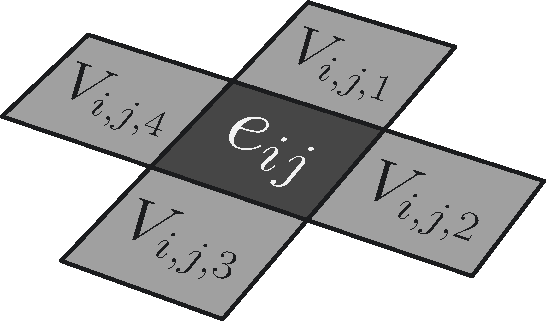
\includegraphics[width = 0.9\linewidth]{puntuacion_elemento}%
	\end{column}
	\end{columns}
	}
\end{frame}


\begin{frame}{Funciones de puntuación}
\begin{block}{\fontsize{18}{18}\selectfont Función: \f{puntuacionGlobal}()}
	\setlength{\abovedisplayshortskip}{0.4cm}
	\setlength{\belowdisplayshortskip}{0.4cm}
	\begin{equation*}
		\f{puntuacionGlobal}\hspace{1.5pt}\textsf{()} = \sum_{i,\hspace{1pt} j}\hspace{1.5pt}\f{puntuacionElemento}\hspace{1.5pt}\textsf{($e_{ij}$)}
	\end{equation*}\,
\end{block}
\end{frame}


\begin{frame}{Algoritmo principal}
	\SetKwIF{If}{ElseIf}{Else}{if}{\!\!:}{else if}{else}{end}%
	\setlength{\algomargin}{0pt}%
	\SetAlgoHangIndent{0pt}%
	%\DecMargin{0.15em}%
	\vskip 3pt%
	\Wider[0.6cm]{%
	\begin{block}{Algoritmo: \textsl{Recocido simulado}}
	\footnotesize%
	\leavevmode%
	\vskip 0.5pt%
	\begin{minipage}[b]{0.465\linewidth}
	\setlength{\algomargin}{13pt}%
	\begin{algorithm}[H]
	\addtolength{\hsize}{\algomargin}%
	\BlankLine
	\Data{\justifying Temperatura inicial $T$, constantes $\alpha$, $a$, $b$, malla con objetos.}
	\OneHalfBlankLine
	\Result{\justifying Malla con objetos acomodados (representada por una matriz de enteros).}
	\TwoBlankLines
	\tcp*[l]{Parámetros del algoritmo.}
	$T = \num[text-family-to-math = true]{50000000}$\;
	$\mathrlap{\alpha}\hphantom{T} = \textsf{0.0000001}$\;
	$\mathrlap{a}\hphantom{T} = \textsf{0.99991}$\;
	$\mathrlap{b}\hphantom{T} = \textsf{1}$\;
	\OneHalfBlankLine
	\tcp*[l]{Puntajes actual y de intercambio.}
	$p_A =\, \f{puntuacionGlobal}()$\;
	$\mathrlap{p_I}\hphantom{p_A} =\, \textsf{0}$%
	\QuarterBlankLine
	\end{algorithm}
	\end{minipage}
	\leavevmode
	\hskip 0.28cm\raisebox{-3.05cm}{\tikz\draw[loosely dotted, line width=0.7pt, color=gray] (0,0) -- (0,6.3);}\hskip 0.28cm%
	\begin{minipage}{0.49\linewidth}
	\setlength{\algomargin}{11pt}%
	\begin{algorithm}[H]
	\addtolength{\hsize}{\algomargin}%
	\setcounter{AlgoLine}{6}%
	\raggedright\While{$T > \frac{b}{1 - a}$}{
		\BlankLine
		\justifying Intercambiar aleatoriamente 2 elementos diferentes en la malla.\;
		\HalfBlankLine
		$p_I = \f{puntuacionGlobal}()$\;
		\HalfBlankLine
		\eIf{$p_A \leq p_I$ \Or $\f{random}([0,1]) < e^{-\frac{{\scriptstyle p}_{\scriptscriptstyle A} -\, {\scriptstyle p}_{\scriptscriptstyle I}}{\alpha T}}$}
		{%
			\BlankLine
			Se acepta el intercambio.\;
			$p_A = p_I$
			\QuarterBlankLine
		}{
			No se acepta el intercambio.
		}
		\HalfBlankLine
		$T = aT + b$
	}%
	\end{algorithm}
	\vspace{0.4cm}%
	\end{minipage}
	\end{block}
	}
\end{frame}


\begin{frame}{Funciones de costo}
	La función de costo utilizada está basada en la que se presenta en el artículo \textsl{Manipulation planning among movable obstacles} \cite{4209604}.
	
	\centering	
	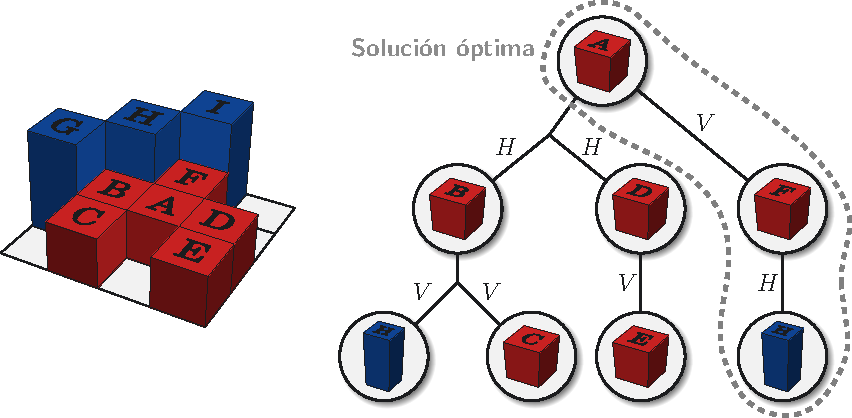
\includegraphics[width = 0.87\textwidth]{arbol}
\end{frame}


\begin{frame}{Funciones de costo}
	\SetAlgoHangIndent{0pt}%
	\SetAlgoSkip{}%
	\SetNlSkip{0.25em}%
	\SetInd{0.2em}{0.45em}%
	%
	\vskip 1.9pt%
	\Wider[0.85cm]{%
	\begin{block}{Función: \f{secuencia}($e_{i j}$, $l$)}
	%\vskip -1pt%
	\footnotesize%
	\centering%
	\begin{algorithm}[H]
	\addtolength{\hsize}{\algomargin}%
	\HalfQuarterBlankLine
	\Data{\justifying Celda $e_{ij}$ del objeto deseado y lista vacía $l$.}
	\QuarterBlankLine
	\Result{\justifying Lista $l$ con la secuencia de elementos a retirar.}
	\QuarterBlankLine
	\Definitions{\justifying $h_{ij}$, $C_{ij}$, $o_{ij}$: altura, clase y datos relevantes del elemento en $e_{ij}$.}
	\vskip 4pt%
	\nonl%
	\begin{minipage}[t]{0.45\linewidth}
	\strut\vspace*{-\baselineskip}\newline%
	\setlength{\algomargin}{0pt}%
	\begin{algorithm}[H]
	\addtolength{\hsize}{1.5cm}%
	\FunctionInicio{$\f{secuencia}(e_{ij},\: l)$}{%
	\BlankLine
		\lIf{$C_{ij} = C_0$}{Finalizar con éxito.}
		\BlankLine
		\uIf{$o_{ij} \not\in l$}{
			\HalfBlankLine
			$\f{append}(o_{ij},\: l)$
			\HalfQuarterBlankLine
			\uIf{$\f{sujetable}(e_{ij})$}{
				\BlankLine
				Finalizar recursión con éxito.
				\HalfBlankLine
			}
			\tcp*[l]{Si no, ejecutar un par:}
			\nonl\nlset{7}%
			\uElseIfWithNoThen{Par 1\normalfont{:}}{
				\QuarterBlankLine
				\SetKwIF{If}{ElseIf}{Else}{if}{\!:}{else if}{else}{end}%
				\lIf{$h_{i+1,\, j} \geq h_{ij}$}{$\f{secuencia}(e_{i+1,\, j},\: l)$}
				\lIf{$h_{i-1,\, j} \geq h_{ij}$}{$\f{secuencia}(e_{i-1,\, j},\: l)$}
				\vskip -1pt%
			}
		}
	}
	\end{algorithm}
	\end{minipage}%
	%
	\begin{minipage}[t]{0.03\linewidth}
	\strut\vspace*{-\baselineskip}\newline%
	\centering\tikz\draw[loosely dotted, line width=0.7pt, color=gray] (0, 0) -- (0, 5);%
	\end{minipage}%
	%
	\begin{minipage}[t]{0.45\linewidth}
	\strut\vspace*{-\baselineskip}\newline%
	\setlength{\algomargin}{13pt}%
	\begin{algorithm}[H]
	\addtolength{\hsize}{1.5cm}%
	\setcounter{AlgoLine}{9}%
	\vspace{-\baselineskip}\noln%
	\SetAlgoNoEnd%
	\FunctionFin{}{
		\vspace{-\baselineskip}\noln%
		\SetAlgoShortEnd%
		\eIfFin{}{%
			\uElseIfWithNoThen{Par 2\hskip 1pt\normalfont{:}}{
				\QuarterBlankLine
				\SetKwIF{If}{ElseIf}{Else}{if}{\!:}{else if}{else}{end}%
				\lIf{$h_{i,\, j+1} \geq h_{ij}$}{$\f{secuencia}(e_{i,\, j+1},\: l)$}
				\lIf{$h_{i,\, j-1} \geq h_{ij}$}{$\f{secuencia}(e_{i,\, j-1},\: l)$}
			}
			\nonl\nlset{13}%
			\Else{
				\tcp*[l]{Si ambos pares fallaron:}
				Finalizar recursión con fallo.
			}
		}{
			Finalizar recursión con fallo.
		}
		Finalizar recursión con éxito.
		\vskip -2pt%
	}\nonl\nlset{20}\textbf{end}
	\vskip -0.5pt%
	\end{algorithm}%
	\end{minipage}%
	\end{algorithm}
	\end{block}
	}
\end{frame}


\begin{frame}{Funciones de costo}
	\vspace{-7pt}%
	\begin{block}{Algoritmo: \itshape Costo $t_{ij}$ de tomar un objeto}
	\footnotesize%
	\SetAlgoHangIndent{0pt}%
	\begin{algorithm}[H]
	\addtolength{\hsize}{\algomargin}%
	\BlankLine
	\Data{Celda $e_{ij}$ del objeto deseado.}
	\HalfBlankLine
	\Result{Costo $t_{ij}$ de tomar el objeto en $e_{ij}$.}
	\HalfBlankLine
	\Definitions{$\f{encontrarTodas}()$: Función de backtracking que retorna todas las soluciones posibles de $\f{secuencia}()$.}
	\BlankLine
	\tcp*[l]{Lista para\! almacenar\! todas\! las\! secuencias\! posibles\! para\! tomar\! un\! objeto.}
	$L = \{ \}$\;
	\HalfBlankLine
	$L = \f{encontrarTodas}(\f{secuencia}(e_{ij},\: l))$\;
	\HalfBlankLine
	$t_{ij} = \min\limits_i \left| L_i \right|$
	%\caption{Algoritmo para calcular el costo $t_{ij}$.}%
	\end{algorithm}
	\end{block}
	%
	\small\setstretch{1.2}%
	\vskip 3pt%
	Como se mencionó, el costo global $T$ es simplemente la suma de los costos individuales $t_{ij}$:
	%
	\fontsize{13}{13}\selectfont%
	\begin{equation*}
		T = \sum_{i,\hspace{1pt} j} \, t_{ij}
	\end{equation*}
\end{frame}
	

\section{Resultados}


\frame[noframenumbering, plain]{\tableofcontents[currentsection]}


\begin{frame}{Tamaños y casos probados}
\begin{columns}[totalwidth = 0.95\textwidth]
\begin{column}{0.45\linewidth}
Tamaños de malla y número de combinaciones de cubos y prismas (casos) probados en estas.
\end{column}
\begin{column}{0.5\linewidth}
\fontsize{14}{14}\selectfont%
\begin{table}[H]
\renewcommand{\arraystretch}{1.4}%
\setlength{\arrayrulewidth}{0.75pt}%
\setlength{\tabcolsep}{0pt}%
\centering%
\begin{tabular}{
	>{\centering} m{0.3\textwidth} 
	>{\centering} m{0.38\textwidth} 
}
	\hline%
	\rule{0pt}{14pt}\bfseries Tamaño malla & \bfseries\#\,Casos probados \tabularnewline 
	\hline%
	3\:$\bm{\times}$\:3 & 32 \tabularnewline 
	3\:$\bm{\times}$\:5 & 85 \tabularnewline 
	4\:$\bm{\times}$\:4 & 88 \tabularnewline
	5\:$\bm{\times}$\:5 & 226 \tabularnewline 
	6\:$\bm{\times}$\:6 & 423 \tabularnewline 
	5\:$\bm{\times}$\:8 & 558 \tabularnewline
	7\:$\bm{\times}$\:7 & 834 \tabularnewline 
	8\:$\bm{\times}$\:8 & 1312 \tabularnewline 
	\hline%
\end{tabular}
\end{table}
\end{column}
\end{columns}
\end{frame}

\captionsetup[figure]{
	labelformat = empty, 
	justification = justified, 
	belowskip = 3pt
}
\setbeamerfont{caption}{size*={12pt}{17pt}}
\tikzset{
	every node/.style = {
		inner sep=0, 
		outer sep=0
	}, 
	arrows = {-Stealth[length=10pt, inset=1pt]}
}

\begin{frame}{Mallas de $\mathsf{3\times 3}$}
	\vfill
	\Wider[1.85cm]{
	\begin{figure}[H]
		% GNUPLOT: LaTeX picture with Postscript
\begingroup
  % Encoding inside the plot.  In the header of your document, this encoding
  % should to defined, e.g., by using
  % \usepackage[latin1,<other encodings>]{inputenc}
  \inputencoding{latin1}%
  \makeatletter
  \providecommand\color[2][]{%
    \GenericError{(gnuplot) \space\space\space\@spaces}{%
      Package color not loaded in conjunction with
      terminal option `colourtext'%
    }{See the gnuplot documentation for explanation.%
    }{Either use 'blacktext' in gnuplot or load the package
      color.sty in LaTeX.}%
    \renewcommand\color[2][]{}%
  }%
  \providecommand\includegraphics[2][]{%
    \GenericError{(gnuplot) \space\space\space\@spaces}{%
      Package graphicx or graphics not loaded%
    }{See the gnuplot documentation for explanation.%
    }{The gnuplot epslatex terminal needs graphicx.sty or graphics.sty.}%
    \renewcommand\includegraphics[2][]{}%
  }%
  \providecommand\rotatebox[2]{#2}%
  \@ifundefined{ifGPcolor}{%
    \newif\ifGPcolor
    \GPcolortrue
  }{}%
  \@ifundefined{ifGPblacktext}{%
    \newif\ifGPblacktext
    \GPblacktexttrue
  }{}%
  % define a \g@addto@macro without @ in the name:
  \let\gplgaddtomacro\g@addto@macro
  % define empty templates for all commands taking text:
  \gdef\gplbacktext{}%
  \gdef\gplfronttext{}%
  \makeatother
  \ifGPblacktext
    % no textcolor at all
    \def\colorrgb#1{}%
    \def\colorgray#1{}%
  \else
    % gray or color?
    \ifGPcolor
      \def\colorrgb#1{\color[rgb]{#1}}%
      \def\colorgray#1{\color[gray]{#1}}%
      \expandafter\def\csname LTw\endcsname{\color{white}}%
      \expandafter\def\csname LTb\endcsname{\color{black}}%
      \expandafter\def\csname LTa\endcsname{\color{black}}%
      \expandafter\def\csname LT0\endcsname{\color[rgb]{1,0,0}}%
      \expandafter\def\csname LT1\endcsname{\color[rgb]{0,1,0}}%
      \expandafter\def\csname LT2\endcsname{\color[rgb]{0,0,1}}%
      \expandafter\def\csname LT3\endcsname{\color[rgb]{1,0,1}}%
      \expandafter\def\csname LT4\endcsname{\color[rgb]{0,1,1}}%
      \expandafter\def\csname LT5\endcsname{\color[rgb]{1,1,0}}%
      \expandafter\def\csname LT6\endcsname{\color[rgb]{0,0,0}}%
      \expandafter\def\csname LT7\endcsname{\color[rgb]{1,0.3,0}}%
      \expandafter\def\csname LT8\endcsname{\color[rgb]{0.5,0.5,0.5}}%
    \else
      % gray
      \def\colorrgb#1{\color{black}}%
      \def\colorgray#1{\color[gray]{#1}}%
      \expandafter\def\csname LTw\endcsname{\color{white}}%
      \expandafter\def\csname LTb\endcsname{\color{black}}%
      \expandafter\def\csname LTa\endcsname{\color{black}}%
      \expandafter\def\csname LT0\endcsname{\color{black}}%
      \expandafter\def\csname LT1\endcsname{\color{black}}%
      \expandafter\def\csname LT2\endcsname{\color{black}}%
      \expandafter\def\csname LT3\endcsname{\color{black}}%
      \expandafter\def\csname LT4\endcsname{\color{black}}%
      \expandafter\def\csname LT5\endcsname{\color{black}}%
      \expandafter\def\csname LT6\endcsname{\color{black}}%
      \expandafter\def\csname LT7\endcsname{\color{black}}%
      \expandafter\def\csname LT8\endcsname{\color{black}}%
    \fi
  \fi
    \setlength{\unitlength}{0.0500bp}%
    \ifx\gptboxheight\undefined%
      \newlength{\gptboxheight}%
      \newlength{\gptboxwidth}%
      \newsavebox{\gptboxtext}%
    \fi%
    \setlength{\fboxrule}{0.5pt}%
    \setlength{\fboxsep}{1pt}%
\begin{picture}(7488.00,4896.00)%
    \gplgaddtomacro\gplbacktext{%
      \csname LTb\endcsname%%
      \put(396,594){\makebox(0,0){\fontsize{8.5}{8.5}\selectfont{4}}}%
      \put(396,1005){\makebox(0,0){\fontsize{8.5}{8.5}\selectfont{6}}}%
      \put(396,1416){\makebox(0,0){\fontsize{8.5}{8.5}\selectfont{8}}}%
      \put(396,1827){\makebox(0,0){\fontsize{8.5}{8.5}\selectfont{10}}}%
      \put(396,2238){\makebox(0,0){\fontsize{8.5}{8.5}\selectfont{12}}}%
      \put(396,2649){\makebox(0,0){\fontsize{8.5}{8.5}\selectfont{14}}}%
      \put(396,3060){\makebox(0,0){\fontsize{8.5}{8.5}\selectfont{16}}}%
      \put(396,3471){\makebox(0,0){\fontsize{8.5}{8.5}\selectfont{18}}}%
      \put(396,3882){\makebox(0,0){\fontsize{8.5}{8.5}\selectfont{20}}}%
      \put(396,4293){\makebox(0,0){\fontsize{8.5}{8.5}\selectfont{22}}}%
      \put(672,396){\rotatebox{45}{\makebox(0,0)[l]{\strut{}\fontsize{5.5}{5.5}\selectfont{8,1}}}}%
      \put(883,396){\rotatebox{45}{\makebox(0,0)[l]{\strut{}\fontsize{5.5}{5.5}\selectfont{7,2}}}}%
      \put(1093,396){\rotatebox{45}{\makebox(0,0)[l]{\strut{}\fontsize{5.5}{5.5}\selectfont{6,3}}}}%
      \put(1304,396){\rotatebox{45}{\makebox(0,0)[l]{\strut{}\fontsize{5.5}{5.5}\selectfont{5,4}}}}%
      \put(1514,396){\rotatebox{45}{\makebox(0,0)[l]{\strut{}\fontsize{5.5}{5.5}\selectfont{4,5}}}}%
      \put(1725,396){\rotatebox{45}{\makebox(0,0)[l]{\strut{}\fontsize{5.5}{5.5}\selectfont{3,6}}}}%
      \put(1935,396){\rotatebox{45}{\makebox(0,0)[l]{\strut{}\fontsize{5.5}{5.5}\selectfont{2,7}}}}%
      \put(2146,396){\rotatebox{45}{\makebox(0,0)[l]{\strut{}\fontsize{5.5}{5.5}\selectfont{1,8}}}}%
      \put(2356,396){\rotatebox{45}{\makebox(0,0)[l]{\strut{}\fontsize{5.5}{5.5}\selectfont{8,0}}}}%
      \put(2567,396){\rotatebox{45}{\makebox(0,0)[l]{\strut{}\fontsize{5.5}{5.5}\selectfont{7,1}}}}%
      \put(2777,396){\rotatebox{45}{\makebox(0,0)[l]{\strut{}\fontsize{5.5}{5.5}\selectfont{6,2}}}}%
      \put(2987,396){\rotatebox{45}{\makebox(0,0)[l]{\strut{}\fontsize{5.5}{5.5}\selectfont{5,3}}}}%
      \put(3198,396){\rotatebox{45}{\makebox(0,0)[l]{\strut{}\fontsize{5.5}{5.5}\selectfont{4,4}}}}%
      \put(3408,396){\rotatebox{45}{\makebox(0,0)[l]{\strut{}\fontsize{5.5}{5.5}\selectfont{3,5}}}}%
      \put(3619,396){\rotatebox{45}{\makebox(0,0)[l]{\strut{}\fontsize{5.5}{5.5}\selectfont{2,6}}}}%
      \put(3829,396){\rotatebox{45}{\makebox(0,0)[l]{\strut{}\fontsize{5.5}{5.5}\selectfont{1,7}}}}%
      \put(4040,396){\rotatebox{45}{\makebox(0,0)[l]{\strut{}\fontsize{5.5}{5.5}\selectfont{0,8}}}}%
      \put(4250,396){\rotatebox{45}{\makebox(0,0)[l]{\strut{}\fontsize{5.5}{5.5}\selectfont{7,0}}}}%
      \put(4461,396){\rotatebox{45}{\makebox(0,0)[l]{\strut{}\fontsize{5.5}{5.5}\selectfont{6,1}}}}%
      \put(4671,396){\rotatebox{45}{\makebox(0,0)[l]{\strut{}\fontsize{5.5}{5.5}\selectfont{5,2}}}}%
      \put(4882,396){\rotatebox{45}{\makebox(0,0)[l]{\strut{}\fontsize{5.5}{5.5}\selectfont{4,3}}}}%
      \put(5092,396){\rotatebox{45}{\makebox(0,0)[l]{\strut{}\fontsize{5.5}{5.5}\selectfont{3,4}}}}%
      \put(5302,396){\rotatebox{45}{\makebox(0,0)[l]{\strut{}\fontsize{5.5}{5.5}\selectfont{2,5}}}}%
      \put(5513,396){\rotatebox{45}{\makebox(0,0)[l]{\strut{}\fontsize{5.5}{5.5}\selectfont{1,6}}}}%
      \put(5723,396){\rotatebox{45}{\makebox(0,0)[l]{\strut{}\fontsize{5.5}{5.5}\selectfont{0,7}}}}%
      \put(5934,396){\rotatebox{45}{\makebox(0,0)[l]{\strut{}\fontsize{5.5}{5.5}\selectfont{6,0}}}}%
      \put(6144,396){\rotatebox{45}{\makebox(0,0)[l]{\strut{}\fontsize{5.5}{5.5}\selectfont{5,1}}}}%
      \put(6355,396){\rotatebox{45}{\makebox(0,0)[l]{\strut{}\fontsize{5.5}{5.5}\selectfont{4,2}}}}%
      \put(6565,396){\rotatebox{45}{\makebox(0,0)[l]{\strut{}\fontsize{5.5}{5.5}\selectfont{3,3}}}}%
      \put(6776,396){\rotatebox{45}{\makebox(0,0)[l]{\strut{}\fontsize{5.5}{5.5}\selectfont{2,4}}}}%
      \put(6986,396){\rotatebox{45}{\makebox(0,0)[l]{\strut{}\fontsize{5.5}{5.5}\selectfont{1,5}}}}%
      \put(7197,396){\rotatebox{45}{\makebox(0,0)[l]{\strut{}\fontsize{5.5}{5.5}\selectfont{0,6}}}}%
      \put(4001,4785){\makebox(0,0){\strut{}\fontsize{13}{13}\selectfont{\textbf{Resultados en mallas de} $\bm{3\times 3}$}}}%
      \put(4001,110){\makebox(0,0){\strut{}\fontsize{12}{12}\selectfont{Objetos en malla (cubos, prismas)}}}%
      \put(66,2547){\rotatebox{90}{\makebox(0,0){\strut{}\fontsize{12}{12}\selectfont{Costo global $T$}}}}%
      \put(7106,3866){\makebox(0,0)[l]{\strut{}}}%
      \csname LTb\endcsname%%
      \put(7245,3866){\makebox(0,0)[l]{\strut{}}}%
      \csname LTb\endcsname%%
      \put(7116,3835){\makebox(0,0)[l]{\strut{}\fontsize{8}{8}\selectfont{,}}}%
    }%
    \gplgaddtomacro\gplfronttext{%
      \csname LTb\endcsname%%
      \put(6886,4272){\makebox(0,0)[r]{\strut{}\fontsize{8}{8}\selectfont{B\'usqueda exhaustiva}}}%
      \csname LTb\endcsname%%
      \put(6886,4052){\makebox(0,0)[r]{\strut{}\fontsize{8}{8}\selectfont{B\'usqueda por RS}}}%
      \csname LTb\endcsname%%
      \put(6886,3832){\makebox(0,0)[r]{\strut{}\fontsize{8}{8}\selectfont{Costo global \'optimo}}}%
    }%
    \gplbacktext
    \put(0,0){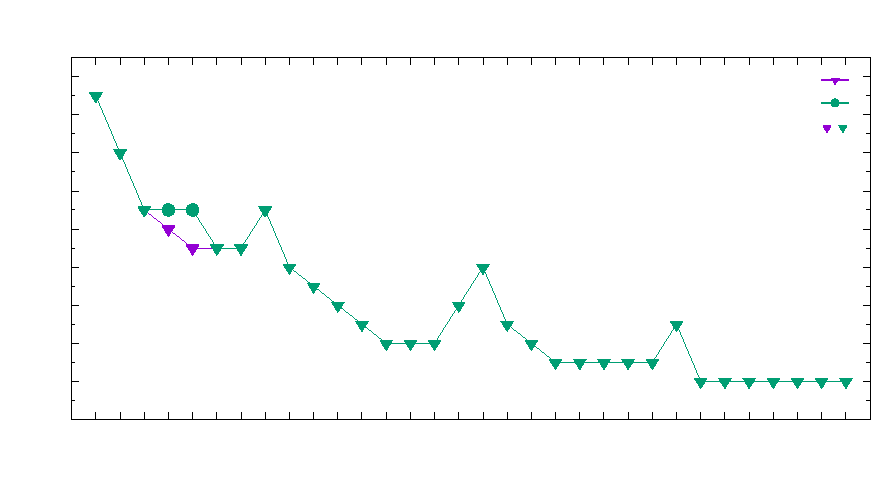
\includegraphics{resultados_3x3}}%
    \gplfronttext
  \end{picture}%
\endgroup
%
	\end{figure}
	}%
\end{frame}

\begin{frame}{Ejemplo ilustrativo en malla de $\mathsf{3\times 3}$}
	\vskip -10pt%
	\begin{figure}[H]
		\caption{Acomodo aleatorio inicial (izquierda) y acomodo encontrado por el algoritmo (derecha), mostrados en diferentes vistas.}%
		\arregloAntesDespues{caso=3x3, separacionAntesDespues=4, separacionVertical=0.4cm}{height=3.3cm}{width=2.565cm}%
	\end{figure}
\end{frame}


\begin{frame}{Mallas de $\mathsf{3\times 5}$}
	\vfill
	\Wider[1.85cm]{
	\begin{figure}[H]
		% GNUPLOT: LaTeX picture with Postscript
\begingroup
  % Encoding inside the plot.  In the header of your document, this encoding
  % should to defined, e.g., by using
  % \usepackage[latin1,<other encodings>]{inputenc}
  \inputencoding{latin1}%
  \makeatletter
  \providecommand\color[2][]{%
    \GenericError{(gnuplot) \space\space\space\@spaces}{%
      Package color not loaded in conjunction with
      terminal option `colourtext'%
    }{See the gnuplot documentation for explanation.%
    }{Either use 'blacktext' in gnuplot or load the package
      color.sty in LaTeX.}%
    \renewcommand\color[2][]{}%
  }%
  \providecommand\includegraphics[2][]{%
    \GenericError{(gnuplot) \space\space\space\@spaces}{%
      Package graphicx or graphics not loaded%
    }{See the gnuplot documentation for explanation.%
    }{The gnuplot epslatex terminal needs graphicx.sty or graphics.sty.}%
    \renewcommand\includegraphics[2][]{}%
  }%
  \providecommand\rotatebox[2]{#2}%
  \@ifundefined{ifGPcolor}{%
    \newif\ifGPcolor
    \GPcolortrue
  }{}%
  \@ifundefined{ifGPblacktext}{%
    \newif\ifGPblacktext
    \GPblacktexttrue
  }{}%
  % define a \g@addto@macro without @ in the name:
  \let\gplgaddtomacro\g@addto@macro
  % define empty templates for all commands taking text:
  \gdef\gplbacktext{}%
  \gdef\gplfronttext{}%
  \makeatother
  \ifGPblacktext
    % no textcolor at all
    \def\colorrgb#1{}%
    \def\colorgray#1{}%
  \else
    % gray or color?
    \ifGPcolor
      \def\colorrgb#1{\color[rgb]{#1}}%
      \def\colorgray#1{\color[gray]{#1}}%
      \expandafter\def\csname LTw\endcsname{\color{white}}%
      \expandafter\def\csname LTb\endcsname{\color{black}}%
      \expandafter\def\csname LTa\endcsname{\color{black}}%
      \expandafter\def\csname LT0\endcsname{\color[rgb]{1,0,0}}%
      \expandafter\def\csname LT1\endcsname{\color[rgb]{0,1,0}}%
      \expandafter\def\csname LT2\endcsname{\color[rgb]{0,0,1}}%
      \expandafter\def\csname LT3\endcsname{\color[rgb]{1,0,1}}%
      \expandafter\def\csname LT4\endcsname{\color[rgb]{0,1,1}}%
      \expandafter\def\csname LT5\endcsname{\color[rgb]{1,1,0}}%
      \expandafter\def\csname LT6\endcsname{\color[rgb]{0,0,0}}%
      \expandafter\def\csname LT7\endcsname{\color[rgb]{1,0.3,0}}%
      \expandafter\def\csname LT8\endcsname{\color[rgb]{0.5,0.5,0.5}}%
    \else
      % gray
      \def\colorrgb#1{\color{black}}%
      \def\colorgray#1{\color[gray]{#1}}%
      \expandafter\def\csname LTw\endcsname{\color{white}}%
      \expandafter\def\csname LTb\endcsname{\color{black}}%
      \expandafter\def\csname LTa\endcsname{\color{black}}%
      \expandafter\def\csname LT0\endcsname{\color{black}}%
      \expandafter\def\csname LT1\endcsname{\color{black}}%
      \expandafter\def\csname LT2\endcsname{\color{black}}%
      \expandafter\def\csname LT3\endcsname{\color{black}}%
      \expandafter\def\csname LT4\endcsname{\color{black}}%
      \expandafter\def\csname LT5\endcsname{\color{black}}%
      \expandafter\def\csname LT6\endcsname{\color{black}}%
      \expandafter\def\csname LT7\endcsname{\color{black}}%
      \expandafter\def\csname LT8\endcsname{\color{black}}%
    \fi
  \fi
    \setlength{\unitlength}{0.0500bp}%
    \ifx\gptboxheight\undefined%
      \newlength{\gptboxheight}%
      \newlength{\gptboxwidth}%
      \newsavebox{\gptboxtext}%
    \fi%
    \setlength{\fboxrule}{0.5pt}%
    \setlength{\fboxsep}{1pt}%
\begin{picture}(8466.00,4320.00)%
    \gplgaddtomacro\gplbacktext{%
      \csname LTb\endcsname%%
      \put(422,1019){\makebox(0,0){\fontsize{8}{8}\selectfont{10}}}%
      \put(422,1958){\makebox(0,0){\fontsize{8}{8}\selectfont{20}}}%
      \put(422,2896){\makebox(0,0){\fontsize{8}{8}\selectfont{30}}}%
      \put(422,3835){\makebox(0,0){\fontsize{8}{8}\selectfont{40}}}%
      \put(733,440){\makebox(0,0){\strut{}\fontsize{7.3}{7.3}\selectfont{13,2}}}%
      \put(1810,440){\makebox(0,0){\strut{}\fontsize{7.3}{7.3}\selectfont{13,1}}}%
      \put(2977,440){\makebox(0,0){\strut{}\fontsize{7.3}{7.3}\selectfont{13,0}}}%
      \put(4233,440){\makebox(0,0){\strut{}\fontsize{7.3}{7.3}\selectfont{12,0}}}%
      \put(5400,440){\makebox(0,0){\strut{}\fontsize{7.3}{7.3}\selectfont{11,0}}}%
      \put(6477,440){\makebox(0,0){\strut{}\fontsize{7.3}{7.3}\selectfont{10,0}}}%
      \put(7464,440){\makebox(0,0){\strut{}\fontsize{7.3}{7.3}\selectfont{9,0}}}%
      \put(8272,440){\makebox(0,0){\strut{}\fontsize{7.3}{7.3}\selectfont{0,9}}}%
      \put(777,3901){\rotatebox{45}{\makebox(0,0)[l]{\strut{}\fontsize{2.5}{2.5}\selectfont{12,3}}}}%
      \put(867,3901){\rotatebox{45}{\makebox(0,0)[l]{\strut{}\fontsize{2.5}{2.5}\selectfont{11,4}}}}%
      \put(957,3901){\rotatebox{45}{\makebox(0,0)[l]{\strut{}\fontsize{2.5}{2.5}\selectfont{10,5}}}}%
      \put(1046,3901){\rotatebox{45}{\makebox(0,0)[l]{\strut{}\fontsize{2.5}{2.5}\selectfont{9,6}}}}%
      \put(1136,3901){\rotatebox{45}{\makebox(0,0)[l]{\strut{}\fontsize{2.5}{2.5}\selectfont{8,7}}}}%
      \put(1226,3901){\rotatebox{45}{\makebox(0,0)[l]{\strut{}\fontsize{2.5}{2.5}\selectfont{7,8}}}}%
      \put(1316,3901){\rotatebox{45}{\makebox(0,0)[l]{\strut{}\fontsize{2.5}{2.5}\selectfont{6,9}}}}%
      \put(1405,3901){\rotatebox{45}{\makebox(0,0)[l]{\strut{}\fontsize{2.5}{2.5}\selectfont{5,10}}}}%
      \put(1495,3901){\rotatebox{45}{\makebox(0,0)[l]{\strut{}\fontsize{2.5}{2.5}\selectfont{4,11}}}}%
      \put(1585,3901){\rotatebox{45}{\makebox(0,0)[l]{\strut{}\fontsize{2.5}{2.5}\selectfont{3,12}}}}%
      \put(1675,3901){\rotatebox{45}{\makebox(0,0)[l]{\strut{}\fontsize{2.5}{2.5}\selectfont{2,13}}}}%
      \put(1854,3901){\rotatebox{45}{\makebox(0,0)[l]{\strut{}\fontsize{2.5}{2.5}\selectfont{12,2}}}}%
      \put(1944,3901){\rotatebox{45}{\makebox(0,0)[l]{\strut{}\fontsize{2.5}{2.5}\selectfont{11,3}}}}%
      \put(2034,3901){\rotatebox{45}{\makebox(0,0)[l]{\strut{}\fontsize{2.5}{2.5}\selectfont{10,4}}}}%
      \put(2123,3901){\rotatebox{45}{\makebox(0,0)[l]{\strut{}\fontsize{2.5}{2.5}\selectfont{9,5}}}}%
      \put(2213,3901){\rotatebox{45}{\makebox(0,0)[l]{\strut{}\fontsize{2.5}{2.5}\selectfont{8,6}}}}%
      \put(2303,3901){\rotatebox{45}{\makebox(0,0)[l]{\strut{}\fontsize{2.5}{2.5}\selectfont{7,7}}}}%
      \put(2393,3901){\rotatebox{45}{\makebox(0,0)[l]{\strut{}\fontsize{2.5}{2.5}\selectfont{6,8}}}}%
      \put(2482,3901){\rotatebox{45}{\makebox(0,0)[l]{\strut{}\fontsize{2.5}{2.5}\selectfont{5,9}}}}%
      \put(2572,3901){\rotatebox{45}{\makebox(0,0)[l]{\strut{}\fontsize{2.5}{2.5}\selectfont{4,10}}}}%
      \put(2662,3901){\rotatebox{45}{\makebox(0,0)[l]{\strut{}\fontsize{2.5}{2.5}\selectfont{3,11}}}}%
      \put(2751,3901){\rotatebox{45}{\makebox(0,0)[l]{\strut{}\fontsize{2.5}{2.5}\selectfont{2,12}}}}%
      \put(2841,3901){\rotatebox{45}{\makebox(0,0)[l]{\strut{}\fontsize{2.5}{2.5}\selectfont{1,13}}}}%
      \put(3021,3901){\rotatebox{45}{\makebox(0,0)[l]{\strut{}\fontsize{2.5}{2.5}\selectfont{12,1}}}}%
      \put(3110,3901){\rotatebox{45}{\makebox(0,0)[l]{\strut{}\fontsize{2.5}{2.5}\selectfont{11,2}}}}%
      \put(3200,3901){\rotatebox{45}{\makebox(0,0)[l]{\strut{}\fontsize{2.5}{2.5}\selectfont{10,3}}}}%
      \put(3290,3901){\rotatebox{45}{\makebox(0,0)[l]{\strut{}\fontsize{2.5}{2.5}\selectfont{9,4}}}}%
      \put(3380,3901){\rotatebox{45}{\makebox(0,0)[l]{\strut{}\fontsize{2.5}{2.5}\selectfont{8,5}}}}%
      \put(3469,3901){\rotatebox{45}{\makebox(0,0)[l]{\strut{}\fontsize{2.5}{2.5}\selectfont{7,6}}}}%
      \put(3559,3901){\rotatebox{45}{\makebox(0,0)[l]{\strut{}\fontsize{2.5}{2.5}\selectfont{6,7}}}}%
      \put(3649,3901){\rotatebox{45}{\makebox(0,0)[l]{\strut{}\fontsize{2.5}{2.5}\selectfont{5,8}}}}%
      \put(3739,3901){\rotatebox{45}{\makebox(0,0)[l]{\strut{}\fontsize{2.5}{2.5}\selectfont{4,9}}}}%
      \put(3828,3901){\rotatebox{45}{\makebox(0,0)[l]{\strut{}\fontsize{2.5}{2.5}\selectfont{3,10}}}}%
      \put(3918,3901){\rotatebox{45}{\makebox(0,0)[l]{\strut{}\fontsize{2.5}{2.5}\selectfont{2,11}}}}%
      \put(4008,3901){\rotatebox{45}{\makebox(0,0)[l]{\strut{}\fontsize{2.5}{2.5}\selectfont{1,12}}}}%
      \put(4098,3901){\rotatebox{45}{\makebox(0,0)[l]{\strut{}\fontsize{2.5}{2.5}\selectfont{0,13}}}}%
      \put(4277,3901){\rotatebox{45}{\makebox(0,0)[l]{\strut{}\fontsize{2.5}{2.5}\selectfont{11,1}}}}%
      \put(4367,3901){\rotatebox{45}{\makebox(0,0)[l]{\strut{}\fontsize{2.5}{2.5}\selectfont{10,2}}}}%
      \put(4457,3901){\rotatebox{45}{\makebox(0,0)[l]{\strut{}\fontsize{2.5}{2.5}\selectfont{9,3}}}}%
      \put(4546,3901){\rotatebox{45}{\makebox(0,0)[l]{\strut{}\fontsize{2.5}{2.5}\selectfont{8,4}}}}%
      \put(4636,3901){\rotatebox{45}{\makebox(0,0)[l]{\strut{}\fontsize{2.5}{2.5}\selectfont{7,5}}}}%
      \put(4726,3901){\rotatebox{45}{\makebox(0,0)[l]{\strut{}\fontsize{2.5}{2.5}\selectfont{6,6}}}}%
      \put(4815,3901){\rotatebox{45}{\makebox(0,0)[l]{\strut{}\fontsize{2.5}{2.5}\selectfont{5,7}}}}%
      \put(4905,3901){\rotatebox{45}{\makebox(0,0)[l]{\strut{}\fontsize{2.5}{2.5}\selectfont{4,8}}}}%
      \put(4995,3901){\rotatebox{45}{\makebox(0,0)[l]{\strut{}\fontsize{2.5}{2.5}\selectfont{3,9}}}}%
      \put(5085,3901){\rotatebox{45}{\makebox(0,0)[l]{\strut{}\fontsize{2.5}{2.5}\selectfont{2,10}}}}%
      \put(5174,3901){\rotatebox{45}{\makebox(0,0)[l]{\strut{}\fontsize{2.5}{2.5}\selectfont{1,11}}}}%
      \put(5264,3901){\rotatebox{45}{\makebox(0,0)[l]{\strut{}\fontsize{2.5}{2.5}\selectfont{0,12}}}}%
      \put(5444,3901){\rotatebox{45}{\makebox(0,0)[l]{\strut{}\fontsize{2.5}{2.5}\selectfont{10,1}}}}%
      \put(5533,3901){\rotatebox{45}{\makebox(0,0)[l]{\strut{}\fontsize{2.5}{2.5}\selectfont{9,2}}}}%
      \put(5623,3901){\rotatebox{45}{\makebox(0,0)[l]{\strut{}\fontsize{2.5}{2.5}\selectfont{8,3}}}}%
      \put(5713,3901){\rotatebox{45}{\makebox(0,0)[l]{\strut{}\fontsize{2.5}{2.5}\selectfont{7,4}}}}%
      \put(5803,3901){\rotatebox{45}{\makebox(0,0)[l]{\strut{}\fontsize{2.5}{2.5}\selectfont{6,5}}}}%
      \put(5892,3901){\rotatebox{45}{\makebox(0,0)[l]{\strut{}\fontsize{2.5}{2.5}\selectfont{5,6}}}}%
      \put(5982,3901){\rotatebox{45}{\makebox(0,0)[l]{\strut{}\fontsize{2.5}{2.5}\selectfont{4,7}}}}%
      \put(6072,3901){\rotatebox{45}{\makebox(0,0)[l]{\strut{}\fontsize{2.5}{2.5}\selectfont{3,8}}}}%
      \put(6162,3901){\rotatebox{45}{\makebox(0,0)[l]{\strut{}\fontsize{2.5}{2.5}\selectfont{2,9}}}}%
      \put(6251,3901){\rotatebox{45}{\makebox(0,0)[l]{\strut{}\fontsize{2.5}{2.5}\selectfont{1,10}}}}%
      \put(6341,3901){\rotatebox{45}{\makebox(0,0)[l]{\strut{}\fontsize{2.5}{2.5}\selectfont{0,11}}}}%
      \put(6520,3901){\rotatebox{45}{\makebox(0,0)[l]{\strut{}\fontsize{2.5}{2.5}\selectfont{9,1}}}}%
      \put(6610,3901){\rotatebox{45}{\makebox(0,0)[l]{\strut{}\fontsize{2.5}{2.5}\selectfont{8,2}}}}%
      \put(6700,3901){\rotatebox{45}{\makebox(0,0)[l]{\strut{}\fontsize{2.5}{2.5}\selectfont{7,3}}}}%
      \put(6790,3901){\rotatebox{45}{\makebox(0,0)[l]{\strut{}\fontsize{2.5}{2.5}\selectfont{6,4}}}}%
      \put(6879,3901){\rotatebox{45}{\makebox(0,0)[l]{\strut{}\fontsize{2.5}{2.5}\selectfont{5,5}}}}%
      \put(6969,3901){\rotatebox{45}{\makebox(0,0)[l]{\strut{}\fontsize{2.5}{2.5}\selectfont{4,6}}}}%
      \put(7059,3901){\rotatebox{45}{\makebox(0,0)[l]{\strut{}\fontsize{2.5}{2.5}\selectfont{3,7}}}}%
      \put(7149,3901){\rotatebox{45}{\makebox(0,0)[l]{\strut{}\fontsize{2.5}{2.5}\selectfont{2,8}}}}%
      \put(7238,3901){\rotatebox{45}{\makebox(0,0)[l]{\strut{}\fontsize{2.5}{2.5}\selectfont{1,9}}}}%
      \put(7328,3901){\rotatebox{45}{\makebox(0,0)[l]{\strut{}\fontsize{2.5}{2.5}\selectfont{0,10}}}}%
      \put(7508,3901){\rotatebox{45}{\makebox(0,0)[l]{\strut{}\fontsize{2.5}{2.5}\selectfont{8,1}}}}%
      \put(7597,3901){\rotatebox{45}{\makebox(0,0)[l]{\strut{}\fontsize{2.5}{2.5}\selectfont{7,2}}}}%
      \put(7687,3901){\rotatebox{45}{\makebox(0,0)[l]{\strut{}\fontsize{2.5}{2.5}\selectfont{6,3}}}}%
      \put(7777,3901){\rotatebox{45}{\makebox(0,0)[l]{\strut{}\fontsize{2.5}{2.5}\selectfont{5,4}}}}%
      \put(7867,3901){\rotatebox{45}{\makebox(0,0)[l]{\strut{}\fontsize{2.5}{2.5}\selectfont{4,5}}}}%
      \put(7956,3901){\rotatebox{45}{\makebox(0,0)[l]{\strut{}\fontsize{2.5}{2.5}\selectfont{3,6}}}}%
      \put(8046,3901){\rotatebox{45}{\makebox(0,0)[l]{\strut{}\fontsize{2.5}{2.5}\selectfont{2,7}}}}%
      \put(8136,3901){\rotatebox{45}{\makebox(0,0)[l]{\strut{}\fontsize{2.5}{2.5}\selectfont{1,8}}}}%
      \put(4503,4209){\makebox(0,0){\strut{}\fontsize{13}{13}\selectfont{\textbf{Resultados en mallas de} $\bm{3\times 5}$}}}%
      \put(4503,110){\makebox(0,0){\strut{}\fontsize{12}{12}\selectfont{Objetos en malla (cubos, prismas)}}}%
      \put(132,2193){\rotatebox{90}{\makebox(0,0){\strut{}\fontsize{12}{12}\selectfont{Costo global $T$}}}}%
      \put(8127,3216){\makebox(0,0)[l]{\strut{}}}%
      \csname LTb\endcsname%%
      \put(8274,3216){\makebox(0,0)[l]{\strut{}}}%
      \csname LTb\endcsname%%
      \put(8143,3185){\makebox(0,0)[l]{\strut{}\fontsize{8}{8}\selectfont{,}}}%
    }%
    \gplgaddtomacro\gplfronttext{%
      \csname LTb\endcsname%%
      \put(7910,3626){\makebox(0,0)[r]{\strut{}\fontsize{8}{8}\selectfont{B\'usqueda exhaustiva}}}%
      \csname LTb\endcsname%%
      \put(7910,3406){\makebox(0,0)[r]{\strut{}\fontsize{8}{8}\selectfont{B\'usqueda por RS}}}%
      \csname LTb\endcsname%%
      \put(7910,3186){\makebox(0,0)[r]{\strut{}\fontsize{8}{8}\selectfont{Costo global \'optimo}}}%
    }%
    \gplgaddtomacro\gplbacktext{%
      \csname LTb\endcsname%%
      \put(687,3901){\rotatebox{45}{\makebox(0,0)[l]{\strut{}\fontsize{2.5}{2.5}\selectfont{13,2}}}}%
      \put(1764,3901){\rotatebox{45}{\makebox(0,0)[l]{\strut{}\fontsize{2.5}{2.5}\selectfont{13,1}}}}%
      \put(2931,3901){\rotatebox{45}{\makebox(0,0)[l]{\strut{}\fontsize{2.5}{2.5}\selectfont{13,0}}}}%
      \put(4187,3901){\rotatebox{45}{\makebox(0,0)[l]{\strut{}\fontsize{2.5}{2.5}\selectfont{12,0}}}}%
      \put(5354,3901){\rotatebox{45}{\makebox(0,0)[l]{\strut{}\fontsize{2.5}{2.5}\selectfont{11,0}}}}%
      \put(6431,3901){\rotatebox{45}{\makebox(0,0)[l]{\strut{}\fontsize{2.5}{2.5}\selectfont{10,0}}}}%
      \put(7418,3901){\rotatebox{45}{\makebox(0,0)[l]{\strut{}\fontsize{2.5}{2.5}\selectfont{9,0}}}}%
      \put(8226,3901){\rotatebox{45}{\makebox(0,0)[l]{\strut{}\fontsize{2.5}{2.5}\selectfont{0,9}}}}%
    }%
    \gplgaddtomacro\gplfronttext{%
    }%
    \gplgaddtomacro\gplbacktext{%
      \csname LTb\endcsname%%
      \put(2393,638){\makebox(0,0){\strut{}\fontsize{5}{5}\selectfont{$N = 14$}}}%
      \put(4816,638){\makebox(0,0){\strut{}\fontsize{5}{5}\selectfont{$N = 12$}}}%
      \put(6969,638){\makebox(0,0){\strut{}\fontsize{5}{5}\selectfont{$N = 10$}}}%
      \put(7867,638){\makebox(0,0){\strut{}\fontsize{5}{5}\selectfont{$N = 9$}}}%
    }%
    \gplgaddtomacro\gplfronttext{%
    }%
    \gplgaddtomacro\gplbacktext{%
      \csname LTb\endcsname%%
      \put(1272,638){\makebox(0,0){\strut{}\fontsize{5}{5}\selectfont{$N = 15$}}}%
      \put(3605,638){\makebox(0,0){\strut{}\fontsize{5}{5}\selectfont{$N = 13$}}}%
      \put(5938,638){\makebox(0,0){\strut{}\fontsize{5}{5}\selectfont{$N = 11$}}}%
    }%
    \gplgaddtomacro\gplfronttext{%
    }%
    \gplbacktext
    \put(0,0){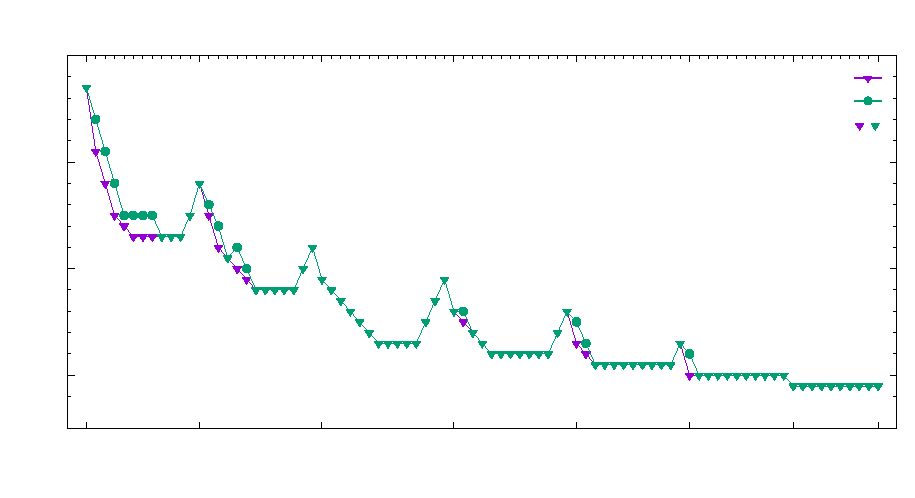
\includegraphics{resultados_3x5}}%
    \gplfronttext
  \end{picture}%
\endgroup
%
	\end{figure}
	}%
\end{frame}

\begin{frame}{Ejemplo ilustrativo en malla de $\mathsf{3\times 5}$}
	\vskip -10pt%
	\begin{figure}[H]
		\caption{Acomodo aleatorio inicial (izquierda) y acomodo encontrado por el algoritmo (derecha), mostrados en diferentes vistas.}%
		\arregloAntesDespues{caso=3x5, separacionAntesDespues=4.3, separacionVertical=0.5cm}{width=4.3cm}[width=4.51717171cm]{width=3.706896cm}%
	\end{figure}%
\end{frame}


\begin{frame}{Mallas de $\mathsf{4\times 4}$}
	\vfill
	\Wider[1.85cm]{
	\begin{figure}[H]
		% GNUPLOT: LaTeX picture with Postscript
\begingroup
  % Encoding inside the plot.  In the header of your document, this encoding
  % should to defined, e.g., by using
  % \usepackage[latin1,<other encodings>]{inputenc}
  \inputencoding{latin1}%
  \makeatletter
  \providecommand\color[2][]{%
    \GenericError{(gnuplot) \space\space\space\@spaces}{%
      Package color not loaded in conjunction with
      terminal option `colourtext'%
    }{See the gnuplot documentation for explanation.%
    }{Either use 'blacktext' in gnuplot or load the package
      color.sty in LaTeX.}%
    \renewcommand\color[2][]{}%
  }%
  \providecommand\includegraphics[2][]{%
    \GenericError{(gnuplot) \space\space\space\@spaces}{%
      Package graphicx or graphics not loaded%
    }{See the gnuplot documentation for explanation.%
    }{The gnuplot epslatex terminal needs graphicx.sty or graphics.sty.}%
    \renewcommand\includegraphics[2][]{}%
  }%
  \providecommand\rotatebox[2]{#2}%
  \@ifundefined{ifGPcolor}{%
    \newif\ifGPcolor
    \GPcolortrue
  }{}%
  \@ifundefined{ifGPblacktext}{%
    \newif\ifGPblacktext
    \GPblacktexttrue
  }{}%
  % define a \g@addto@macro without @ in the name:
  \let\gplgaddtomacro\g@addto@macro
  % define empty templates for all commands taking text:
  \gdef\gplbacktext{}%
  \gdef\gplfronttext{}%
  \makeatother
  \ifGPblacktext
    % no textcolor at all
    \def\colorrgb#1{}%
    \def\colorgray#1{}%
  \else
    % gray or color?
    \ifGPcolor
      \def\colorrgb#1{\color[rgb]{#1}}%
      \def\colorgray#1{\color[gray]{#1}}%
      \expandafter\def\csname LTw\endcsname{\color{white}}%
      \expandafter\def\csname LTb\endcsname{\color{black}}%
      \expandafter\def\csname LTa\endcsname{\color{black}}%
      \expandafter\def\csname LT0\endcsname{\color[rgb]{1,0,0}}%
      \expandafter\def\csname LT1\endcsname{\color[rgb]{0,1,0}}%
      \expandafter\def\csname LT2\endcsname{\color[rgb]{0,0,1}}%
      \expandafter\def\csname LT3\endcsname{\color[rgb]{1,0,1}}%
      \expandafter\def\csname LT4\endcsname{\color[rgb]{0,1,1}}%
      \expandafter\def\csname LT5\endcsname{\color[rgb]{1,1,0}}%
      \expandafter\def\csname LT6\endcsname{\color[rgb]{0,0,0}}%
      \expandafter\def\csname LT7\endcsname{\color[rgb]{1,0.3,0}}%
      \expandafter\def\csname LT8\endcsname{\color[rgb]{0.5,0.5,0.5}}%
    \else
      % gray
      \def\colorrgb#1{\color{black}}%
      \def\colorgray#1{\color[gray]{#1}}%
      \expandafter\def\csname LTw\endcsname{\color{white}}%
      \expandafter\def\csname LTb\endcsname{\color{black}}%
      \expandafter\def\csname LTa\endcsname{\color{black}}%
      \expandafter\def\csname LT0\endcsname{\color{black}}%
      \expandafter\def\csname LT1\endcsname{\color{black}}%
      \expandafter\def\csname LT2\endcsname{\color{black}}%
      \expandafter\def\csname LT3\endcsname{\color{black}}%
      \expandafter\def\csname LT4\endcsname{\color{black}}%
      \expandafter\def\csname LT5\endcsname{\color{black}}%
      \expandafter\def\csname LT6\endcsname{\color{black}}%
      \expandafter\def\csname LT7\endcsname{\color{black}}%
      \expandafter\def\csname LT8\endcsname{\color{black}}%
    \fi
  \fi
    \setlength{\unitlength}{0.0500bp}%
    \ifx\gptboxheight\undefined%
      \newlength{\gptboxheight}%
      \newlength{\gptboxwidth}%
      \newsavebox{\gptboxtext}%
    \fi%
    \setlength{\fboxrule}{0.5pt}%
    \setlength{\fboxsep}{1pt}%
\begin{picture}(8466.00,4464.00)%
    \gplgaddtomacro\gplbacktext{%
      \csname LTb\endcsname%%
      \put(356,1018){\makebox(0,0){\fontsize{9}{9}\selectfont{10}}}%
      \put(356,2042){\makebox(0,0){\fontsize{9}{9}\selectfont{20}}}%
      \put(356,3065){\makebox(0,0){\fontsize{9}{9}\selectfont{30}}}%
      \put(356,4089){\makebox(0,0){\fontsize{9}{9}\selectfont{40}}}%
      \put(663,396){\makebox(0,0){\strut{}\fontsize{8.0001}{8.0001}\selectfont{12,4}}}%
      \put(1451,396){\makebox(0,0){\strut{}\fontsize{8.0001}{8.0001}\selectfont{12,3}}}%
      \put(2326,396){\makebox(0,0){\strut{}\fontsize{8.0001}{8.0001}\selectfont{12,2}}}%
      \put(3288,396){\makebox(0,0){\strut{}\fontsize{8.0001}{8.0001}\selectfont{12,1}}}%
      \put(4338,396){\makebox(0,0){\strut{}\fontsize{8.0001}{8.0001}\selectfont{12,0}}}%
      \put(5476,396){\makebox(0,0){\strut{}\fontsize{8.0001}{8.0001}\selectfont{11,0}}}%
      \put(6526,396){\makebox(0,0){\strut{}\fontsize{8.0001}{8.0001}\selectfont{10,0}}}%
      \put(7488,396){\makebox(0,0){\strut{}\fontsize{8.0001}{8.0001}\selectfont{9,0}}}%
      \put(8276,396){\makebox(0,0){\strut{}\fontsize{8.0001}{8.0001}\selectfont{0,9}}}%
      \put(705,4155){\rotatebox{45}{\makebox(0,0)[l]{\strut{}\fontsize{2.5}{2.5}\selectfont{11,5}}}}%
      \put(792,4155){\rotatebox{45}{\makebox(0,0)[l]{\strut{}\fontsize{2.5}{2.5}\selectfont{10,6}}}}%
      \put(880,4155){\rotatebox{45}{\makebox(0,0)[l]{\strut{}\fontsize{2.5}{2.5}\selectfont{9,7}}}}%
      \put(967,4155){\rotatebox{45}{\makebox(0,0)[l]{\strut{}\fontsize{2.5}{2.5}\selectfont{8,8}}}}%
      \put(1055,4155){\rotatebox{45}{\makebox(0,0)[l]{\strut{}\fontsize{2.5}{2.5}\selectfont{7,9}}}}%
      \put(1142,4155){\rotatebox{45}{\makebox(0,0)[l]{\strut{}\fontsize{2.5}{2.5}\selectfont{6,10}}}}%
      \put(1230,4155){\rotatebox{45}{\makebox(0,0)[l]{\strut{}\fontsize{2.5}{2.5}\selectfont{5,11}}}}%
      \put(1317,4155){\rotatebox{45}{\makebox(0,0)[l]{\strut{}\fontsize{2.5}{2.5}\selectfont{4,12}}}}%
      \put(1492,4155){\rotatebox{45}{\makebox(0,0)[l]{\strut{}\fontsize{2.5}{2.5}\selectfont{11,4}}}}%
      \put(1580,4155){\rotatebox{45}{\makebox(0,0)[l]{\strut{}\fontsize{2.5}{2.5}\selectfont{10,5}}}}%
      \put(1667,4155){\rotatebox{45}{\makebox(0,0)[l]{\strut{}\fontsize{2.5}{2.5}\selectfont{9,6}}}}%
      \put(1755,4155){\rotatebox{45}{\makebox(0,0)[l]{\strut{}\fontsize{2.5}{2.5}\selectfont{8,7}}}}%
      \put(1842,4155){\rotatebox{45}{\makebox(0,0)[l]{\strut{}\fontsize{2.5}{2.5}\selectfont{7,8}}}}%
      \put(1930,4155){\rotatebox{45}{\makebox(0,0)[l]{\strut{}\fontsize{2.5}{2.5}\selectfont{6,9}}}}%
      \put(2017,4155){\rotatebox{45}{\makebox(0,0)[l]{\strut{}\fontsize{2.5}{2.5}\selectfont{5,10}}}}%
      \put(2105,4155){\rotatebox{45}{\makebox(0,0)[l]{\strut{}\fontsize{2.5}{2.5}\selectfont{4,11}}}}%
      \put(2192,4155){\rotatebox{45}{\makebox(0,0)[l]{\strut{}\fontsize{2.5}{2.5}\selectfont{3,12}}}}%
      \put(2367,4155){\rotatebox{45}{\makebox(0,0)[l]{\strut{}\fontsize{2.5}{2.5}\selectfont{11,3}}}}%
      \put(2455,4155){\rotatebox{45}{\makebox(0,0)[l]{\strut{}\fontsize{2.5}{2.5}\selectfont{10,4}}}}%
      \put(2542,4155){\rotatebox{45}{\makebox(0,0)[l]{\strut{}\fontsize{2.5}{2.5}\selectfont{9,5}}}}%
      \put(2630,4155){\rotatebox{45}{\makebox(0,0)[l]{\strut{}\fontsize{2.5}{2.5}\selectfont{8,6}}}}%
      \put(2717,4155){\rotatebox{45}{\makebox(0,0)[l]{\strut{}\fontsize{2.5}{2.5}\selectfont{7,7}}}}%
      \put(2805,4155){\rotatebox{45}{\makebox(0,0)[l]{\strut{}\fontsize{2.5}{2.5}\selectfont{6,8}}}}%
      \put(2892,4155){\rotatebox{45}{\makebox(0,0)[l]{\strut{}\fontsize{2.5}{2.5}\selectfont{5,9}}}}%
      \put(2980,4155){\rotatebox{45}{\makebox(0,0)[l]{\strut{}\fontsize{2.5}{2.5}\selectfont{4,10}}}}%
      \put(3067,4155){\rotatebox{45}{\makebox(0,0)[l]{\strut{}\fontsize{2.5}{2.5}\selectfont{3,11}}}}%
      \put(3155,4155){\rotatebox{45}{\makebox(0,0)[l]{\strut{}\fontsize{2.5}{2.5}\selectfont{2,12}}}}%
      \put(3330,4155){\rotatebox{45}{\makebox(0,0)[l]{\strut{}\fontsize{2.5}{2.5}\selectfont{11,2}}}}%
      \put(3417,4155){\rotatebox{45}{\makebox(0,0)[l]{\strut{}\fontsize{2.5}{2.5}\selectfont{10,3}}}}%
      \put(3505,4155){\rotatebox{45}{\makebox(0,0)[l]{\strut{}\fontsize{2.5}{2.5}\selectfont{9,4}}}}%
      \put(3592,4155){\rotatebox{45}{\makebox(0,0)[l]{\strut{}\fontsize{2.5}{2.5}\selectfont{8,5}}}}%
      \put(3680,4155){\rotatebox{45}{\makebox(0,0)[l]{\strut{}\fontsize{2.5}{2.5}\selectfont{7,6}}}}%
      \put(3767,4155){\rotatebox{45}{\makebox(0,0)[l]{\strut{}\fontsize{2.5}{2.5}\selectfont{6,7}}}}%
      \put(3855,4155){\rotatebox{45}{\makebox(0,0)[l]{\strut{}\fontsize{2.5}{2.5}\selectfont{5,8}}}}%
      \put(3942,4155){\rotatebox{45}{\makebox(0,0)[l]{\strut{}\fontsize{2.5}{2.5}\selectfont{4,9}}}}%
      \put(4030,4155){\rotatebox{45}{\makebox(0,0)[l]{\strut{}\fontsize{2.5}{2.5}\selectfont{3,10}}}}%
      \put(4117,4155){\rotatebox{45}{\makebox(0,0)[l]{\strut{}\fontsize{2.5}{2.5}\selectfont{2,11}}}}%
      \put(4205,4155){\rotatebox{45}{\makebox(0,0)[l]{\strut{}\fontsize{2.5}{2.5}\selectfont{1,12}}}}%
      \put(4380,4155){\rotatebox{45}{\makebox(0,0)[l]{\strut{}\fontsize{2.5}{2.5}\selectfont{11,1}}}}%
      \put(4467,4155){\rotatebox{45}{\makebox(0,0)[l]{\strut{}\fontsize{2.5}{2.5}\selectfont{10,2}}}}%
      \put(4555,4155){\rotatebox{45}{\makebox(0,0)[l]{\strut{}\fontsize{2.5}{2.5}\selectfont{9,3}}}}%
      \put(4642,4155){\rotatebox{45}{\makebox(0,0)[l]{\strut{}\fontsize{2.5}{2.5}\selectfont{8,4}}}}%
      \put(4730,4155){\rotatebox{45}{\makebox(0,0)[l]{\strut{}\fontsize{2.5}{2.5}\selectfont{7,5}}}}%
      \put(4817,4155){\rotatebox{45}{\makebox(0,0)[l]{\strut{}\fontsize{2.5}{2.5}\selectfont{6,6}}}}%
      \put(4905,4155){\rotatebox{45}{\makebox(0,0)[l]{\strut{}\fontsize{2.5}{2.5}\selectfont{5,7}}}}%
      \put(4992,4155){\rotatebox{45}{\makebox(0,0)[l]{\strut{}\fontsize{2.5}{2.5}\selectfont{4,8}}}}%
      \put(5080,4155){\rotatebox{45}{\makebox(0,0)[l]{\strut{}\fontsize{2.5}{2.5}\selectfont{3,9}}}}%
      \put(5167,4155){\rotatebox{45}{\makebox(0,0)[l]{\strut{}\fontsize{2.5}{2.5}\selectfont{2,10}}}}%
      \put(5255,4155){\rotatebox{45}{\makebox(0,0)[l]{\strut{}\fontsize{2.5}{2.5}\selectfont{1,11}}}}%
      \put(5342,4155){\rotatebox{45}{\makebox(0,0)[l]{\strut{}\fontsize{2.5}{2.5}\selectfont{0,12}}}}%
      \put(5517,4155){\rotatebox{45}{\makebox(0,0)[l]{\strut{}\fontsize{2.5}{2.5}\selectfont{10,1}}}}%
      \put(5605,4155){\rotatebox{45}{\makebox(0,0)[l]{\strut{}\fontsize{2.5}{2.5}\selectfont{9,2}}}}%
      \put(5692,4155){\rotatebox{45}{\makebox(0,0)[l]{\strut{}\fontsize{2.5}{2.5}\selectfont{8,3}}}}%
      \put(5780,4155){\rotatebox{45}{\makebox(0,0)[l]{\strut{}\fontsize{2.5}{2.5}\selectfont{7,4}}}}%
      \put(5867,4155){\rotatebox{45}{\makebox(0,0)[l]{\strut{}\fontsize{2.5}{2.5}\selectfont{6,5}}}}%
      \put(5955,4155){\rotatebox{45}{\makebox(0,0)[l]{\strut{}\fontsize{2.5}{2.5}\selectfont{5,6}}}}%
      \put(6042,4155){\rotatebox{45}{\makebox(0,0)[l]{\strut{}\fontsize{2.5}{2.5}\selectfont{4,7}}}}%
      \put(6130,4155){\rotatebox{45}{\makebox(0,0)[l]{\strut{}\fontsize{2.5}{2.5}\selectfont{3,8}}}}%
      \put(6217,4155){\rotatebox{45}{\makebox(0,0)[l]{\strut{}\fontsize{2.5}{2.5}\selectfont{2,9}}}}%
      \put(6305,4155){\rotatebox{45}{\makebox(0,0)[l]{\strut{}\fontsize{2.5}{2.5}\selectfont{1,10}}}}%
      \put(6392,4155){\rotatebox{45}{\makebox(0,0)[l]{\strut{}\fontsize{2.5}{2.5}\selectfont{0,11}}}}%
      \put(6567,4155){\rotatebox{45}{\makebox(0,0)[l]{\strut{}\fontsize{2.5}{2.5}\selectfont{9,1}}}}%
      \put(6655,4155){\rotatebox{45}{\makebox(0,0)[l]{\strut{}\fontsize{2.5}{2.5}\selectfont{8,2}}}}%
      \put(6742,4155){\rotatebox{45}{\makebox(0,0)[l]{\strut{}\fontsize{2.5}{2.5}\selectfont{7,3}}}}%
      \put(6830,4155){\rotatebox{45}{\makebox(0,0)[l]{\strut{}\fontsize{2.5}{2.5}\selectfont{6,4}}}}%
      \put(6917,4155){\rotatebox{45}{\makebox(0,0)[l]{\strut{}\fontsize{2.5}{2.5}\selectfont{5,5}}}}%
      \put(7005,4155){\rotatebox{45}{\makebox(0,0)[l]{\strut{}\fontsize{2.5}{2.5}\selectfont{4,6}}}}%
      \put(7092,4155){\rotatebox{45}{\makebox(0,0)[l]{\strut{}\fontsize{2.5}{2.5}\selectfont{3,7}}}}%
      \put(7180,4155){\rotatebox{45}{\makebox(0,0)[l]{\strut{}\fontsize{2.5}{2.5}\selectfont{2,8}}}}%
      \put(7267,4155){\rotatebox{45}{\makebox(0,0)[l]{\strut{}\fontsize{2.5}{2.5}\selectfont{1,9}}}}%
      \put(7355,4155){\rotatebox{45}{\makebox(0,0)[l]{\strut{}\fontsize{2.5}{2.5}\selectfont{0,10}}}}%
      \put(7530,4155){\rotatebox{45}{\makebox(0,0)[l]{\strut{}\fontsize{2.5}{2.5}\selectfont{8,1}}}}%
      \put(7617,4155){\rotatebox{45}{\makebox(0,0)[l]{\strut{}\fontsize{2.5}{2.5}\selectfont{7,2}}}}%
      \put(7705,4155){\rotatebox{45}{\makebox(0,0)[l]{\strut{}\fontsize{2.5}{2.5}\selectfont{6,3}}}}%
      \put(7792,4155){\rotatebox{45}{\makebox(0,0)[l]{\strut{}\fontsize{2.5}{2.5}\selectfont{5,4}}}}%
      \put(7880,4155){\rotatebox{45}{\makebox(0,0)[l]{\strut{}\fontsize{2.5}{2.5}\selectfont{4,5}}}}%
      \put(7967,4155){\rotatebox{45}{\makebox(0,0)[l]{\strut{}\fontsize{2.5}{2.5}\selectfont{3,6}}}}%
      \put(8055,4155){\rotatebox{45}{\makebox(0,0)[l]{\strut{}\fontsize{2.5}{2.5}\selectfont{2,7}}}}%
      \put(8142,4155){\rotatebox{45}{\makebox(0,0)[l]{\strut{}\fontsize{2.5}{2.5}\selectfont{1,8}}}}%
      \put(4470,4353){\makebox(0,0){\strut{}\fontsize{13}{13}\selectfont{Resultados en mallas de 4 $\times$ 4}}}%
      \put(4470,110){\makebox(0,0){\strut{}\fontsize{11}{11}\selectfont{Objetos en malla (cubos, prismas)}}}%
      \put(66,2298){\rotatebox{90}{\makebox(0,0){\strut{}\fontsize{11}{11}\selectfont{Costo global $T$}}}}%
      \put(8124,3446){\makebox(0,0)[l]{\strut{}}}%
      \csname LTb\endcsname%%
      \put(8273,3446){\makebox(0,0)[l]{\strut{}}}%
      \csname LTb\endcsname%%
      \put(8140,3433){\makebox(0,0)[l]{\strut{}\fontsize{8.5}{8.5}\selectfont{,}}}%
    }%
    \gplgaddtomacro\gplfronttext{%
      \csname LTb\endcsname%%
      \put(7910,3872){\makebox(0,0)[r]{\strut{}\fontsize{8.5}{8.5}\selectfont{B\'usqueda exhaustiva}}}%
      \csname LTb\endcsname%%
      \put(7910,3652){\makebox(0,0)[r]{\strut{}\fontsize{8.5}{8.5}\selectfont{B\'usqueda por RS}}}%
      \csname LTb\endcsname%%
      \put(7910,3432){\makebox(0,0)[r]{\strut{}\fontsize{8.5}{8.5}\selectfont{Costo global \'optimo}}}%
    }%
    \gplgaddtomacro\gplbacktext{%
      \csname LTb\endcsname%%
      \put(617,4155){\rotatebox{45}{\makebox(0,0)[l]{\strut{}\fontsize{2.5}{2.5}\selectfont{12,4}}}}%
      \put(1405,4155){\rotatebox{45}{\makebox(0,0)[l]{\strut{}\fontsize{2.5}{2.5}\selectfont{12,3}}}}%
      \put(2280,4155){\rotatebox{45}{\makebox(0,0)[l]{\strut{}\fontsize{2.5}{2.5}\selectfont{12,2}}}}%
      \put(3242,4155){\rotatebox{45}{\makebox(0,0)[l]{\strut{}\fontsize{2.5}{2.5}\selectfont{12,1}}}}%
      \put(4292,4155){\rotatebox{45}{\makebox(0,0)[l]{\strut{}\fontsize{2.5}{2.5}\selectfont{12,0}}}}%
      \put(5430,4155){\rotatebox{45}{\makebox(0,0)[l]{\strut{}\fontsize{2.5}{2.5}\selectfont{11,0}}}}%
      \put(6480,4155){\rotatebox{45}{\makebox(0,0)[l]{\strut{}\fontsize{2.5}{2.5}\selectfont{10,0}}}}%
      \put(7442,4155){\rotatebox{45}{\makebox(0,0)[l]{\strut{}\fontsize{2.5}{2.5}\selectfont{9,0}}}}%
      \put(8230,4155){\rotatebox{45}{\makebox(0,0)[l]{\strut{}\fontsize{2.5}{2.5}\selectfont{0,9}}}}%
    }%
    \gplgaddtomacro\gplfronttext{%
    }%
    \gplgaddtomacro\gplbacktext{%
      \csname LTb\endcsname%%
      \put(1056,616){\makebox(0,0){\strut{}\fontsize{5}{5}\selectfont{$N =$ \tiny 16}}}%
      \put(2806,616){\makebox(0,0){\strut{}\fontsize{5}{5}\selectfont{$N =$ \tiny 14}}}%
      \put(4906,616){\makebox(0,0){\strut{}\fontsize{5}{5}\selectfont{$N =$ \tiny 12}}}%
      \put(7006,616){\makebox(0,0){\strut{}\fontsize{5}{5}\selectfont{$N =$ \tiny 10}}}%
      \put(7881,616){\makebox(0,0){\strut{}\fontsize{5}{5}\selectfont{$N =$ \tiny 9}}}%
    }%
    \gplgaddtomacro\gplfronttext{%
    }%
    \gplgaddtomacro\gplbacktext{%
      \csname LTb\endcsname%%
      \put(1888,616){\makebox(0,0){\strut{}\fontsize{5}{5}\selectfont{$N =$ \tiny 15}}}%
      \put(3813,616){\makebox(0,0){\strut{}\fontsize{5}{5}\selectfont{$N =$ \tiny 13}}}%
      \put(6001,616){\makebox(0,0){\strut{}\fontsize{5}{5}\selectfont{$N =$ \tiny 11}}}%
    }%
    \gplgaddtomacro\gplfronttext{%
    }%
    \gplbacktext
    \put(0,0){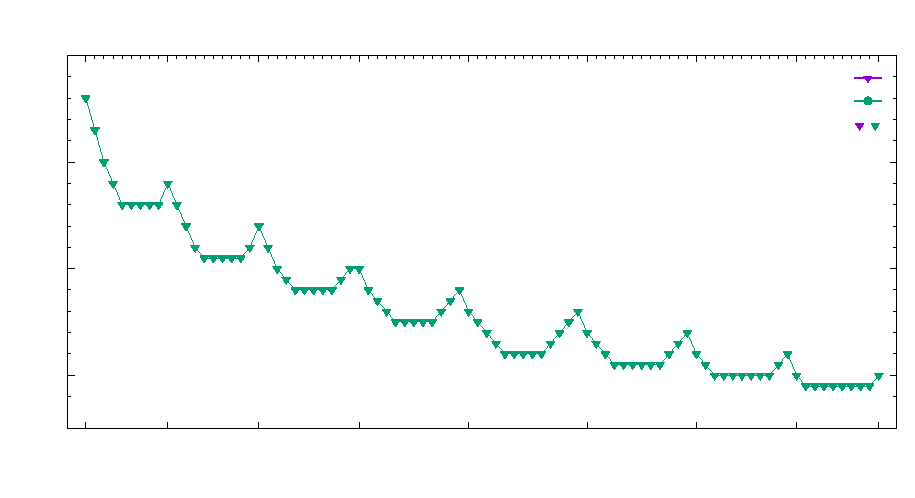
\includegraphics{resultados_4x4}}%
    \gplfronttext
  \end{picture}%
\endgroup
%
	\end{figure}
	}%
\end{frame}

\begin{frame}{Ejemplo ilustrativo en malla de $\mathsf{4\times 4}$}
	\vskip -8pt%
	\begin{figure}[H]
		\caption{Acomodo aleatorio inicial (izquierda) y acomodo encontrado por el algoritmo (derecha), mostrados en diferentes vistas.}%
		\arregloAntesDespues{caso=4x4, separacionAntesDespues=4, separacionVertical=0.35cm}{width=3.9cm}[width=3.94321cm]{width=2.8cm}%
	\end{figure}
\end{frame}


\begin{frame}{Mallas de $\mathsf{5\times 5}$}
	\vfill
	\Wider[1.85cm]{
	\begin{figure}[H]
		% GNUPLOT: LaTeX picture with Postscript
\begingroup
  % Encoding inside the plot.  In the header of your document, this encoding
  % should to defined, e.g., by using
  % \usepackage[latin1,<other encodings>]{inputenc}
  \inputencoding{latin1}%
  \makeatletter
  \providecommand\color[2][]{%
    \GenericError{(gnuplot) \space\space\space\@spaces}{%
      Package color not loaded in conjunction with
      terminal option `colourtext'%
    }{See the gnuplot documentation for explanation.%
    }{Either use 'blacktext' in gnuplot or load the package
      color.sty in LaTeX.}%
    \renewcommand\color[2][]{}%
  }%
  \providecommand\includegraphics[2][]{%
    \GenericError{(gnuplot) \space\space\space\@spaces}{%
      Package graphicx or graphics not loaded%
    }{See the gnuplot documentation for explanation.%
    }{The gnuplot epslatex terminal needs graphicx.sty or graphics.sty.}%
    \renewcommand\includegraphics[2][]{}%
  }%
  \providecommand\rotatebox[2]{#2}%
  \@ifundefined{ifGPcolor}{%
    \newif\ifGPcolor
    \GPcolortrue
  }{}%
  \@ifundefined{ifGPblacktext}{%
    \newif\ifGPblacktext
    \GPblacktexttrue
  }{}%
  % define a \g@addto@macro without @ in the name:
  \let\gplgaddtomacro\g@addto@macro
  % define empty templates for all commands taking text:
  \gdef\gplbacktext{}%
  \gdef\gplfronttext{}%
  \makeatother
  \ifGPblacktext
    % no textcolor at all
    \def\colorrgb#1{}%
    \def\colorgray#1{}%
  \else
    % gray or color?
    \ifGPcolor
      \def\colorrgb#1{\color[rgb]{#1}}%
      \def\colorgray#1{\color[gray]{#1}}%
      \expandafter\def\csname LTw\endcsname{\color{white}}%
      \expandafter\def\csname LTb\endcsname{\color{black}}%
      \expandafter\def\csname LTa\endcsname{\color{black}}%
      \expandafter\def\csname LT0\endcsname{\color[rgb]{1,0,0}}%
      \expandafter\def\csname LT1\endcsname{\color[rgb]{0,1,0}}%
      \expandafter\def\csname LT2\endcsname{\color[rgb]{0,0,1}}%
      \expandafter\def\csname LT3\endcsname{\color[rgb]{1,0,1}}%
      \expandafter\def\csname LT4\endcsname{\color[rgb]{0,1,1}}%
      \expandafter\def\csname LT5\endcsname{\color[rgb]{1,1,0}}%
      \expandafter\def\csname LT6\endcsname{\color[rgb]{0,0,0}}%
      \expandafter\def\csname LT7\endcsname{\color[rgb]{1,0.3,0}}%
      \expandafter\def\csname LT8\endcsname{\color[rgb]{0.5,0.5,0.5}}%
    \else
      % gray
      \def\colorrgb#1{\color{black}}%
      \def\colorgray#1{\color[gray]{#1}}%
      \expandafter\def\csname LTw\endcsname{\color{white}}%
      \expandafter\def\csname LTb\endcsname{\color{black}}%
      \expandafter\def\csname LTa\endcsname{\color{black}}%
      \expandafter\def\csname LT0\endcsname{\color{black}}%
      \expandafter\def\csname LT1\endcsname{\color{black}}%
      \expandafter\def\csname LT2\endcsname{\color{black}}%
      \expandafter\def\csname LT3\endcsname{\color{black}}%
      \expandafter\def\csname LT4\endcsname{\color{black}}%
      \expandafter\def\csname LT5\endcsname{\color{black}}%
      \expandafter\def\csname LT6\endcsname{\color{black}}%
      \expandafter\def\csname LT7\endcsname{\color{black}}%
      \expandafter\def\csname LT8\endcsname{\color{black}}%
    \fi
  \fi
    \setlength{\unitlength}{0.0500bp}%
    \ifx\gptboxheight\undefined%
      \newlength{\gptboxheight}%
      \newlength{\gptboxwidth}%
      \newsavebox{\gptboxtext}%
    \fi%
    \setlength{\fboxrule}{0.5pt}%
    \setlength{\fboxsep}{1pt}%
\begin{picture}(8466.00,4464.00)%
    \gplgaddtomacro\gplbacktext{%
      \csname LTb\endcsname%%
      \put(356,506){\makebox(0,0){\strut{}\raisebox{2pt}{\fontsize{9}{9}\selectfont{10}}}}%
      \put(356,4032){\makebox(0,0){\strut{}\raisebox{2pt}{\fontsize{9}{9}\selectfont{$\infty$}}}}%
      \put(356,1010){\makebox(0,0){\fontsize{9}{9}\selectfont{20}}}%
      \put(356,1514){\makebox(0,0){\fontsize{9}{9}\selectfont{30}}}%
      \put(356,2017){\makebox(0,0){\fontsize{9}{9}\selectfont{40}}}%
      \put(356,2521){\makebox(0,0){\fontsize{9}{9}\selectfont{50}}}%
      \put(356,3025){\makebox(0,0){\fontsize{9}{9}\selectfont{60}}}%
      \put(356,3529){\makebox(0,0){\fontsize{9}{9}\selectfont{70}}}%
      \put(558,396){\makebox(0,0){\strut{}\fontsize{8.0001}{8.0001}\selectfont{21,4}}}%
      \put(1183,396){\makebox(0,0){\strut{}\fontsize{8.0001}{8.0001}\selectfont{21,3}}}%
      \put(1844,396){\makebox(0,0){\strut{}\fontsize{8.0001}{8.0001}\selectfont{21,2}}}%
      \put(2540,396){\makebox(0,0){\strut{}\fontsize{8.0001}{8.0001}\selectfont{21,1}}}%
      \put(3270,396){\makebox(0,0){\strut{}\fontsize{8.0001}{8.0001}\selectfont{21,0}}}%
      \put(4035,396){\makebox(0,0){\strut{}\fontsize{8.0001}{8.0001}\selectfont{20,0}}}%
      \put(4765,396){\makebox(0,0){\strut{}\fontsize{8.0001}{8.0001}\selectfont{19,0}}}%
      \put(5461,396){\makebox(0,0){\strut{}\fontsize{8.0001}{8.0001}\selectfont{18,0}}}%
      \put(6121,396){\makebox(0,0){\strut{}\fontsize{8.0001}{8.0001}\selectfont{17,0}}}%
      \put(6747,396){\makebox(0,0){\strut{}\fontsize{8.0001}{8.0001}\selectfont{16,0}}}%
      \put(7338,396){\makebox(0,0){\strut{}\fontsize{8.0001}{8.0001}\selectfont{15,0}}}%
      \put(7895,396){\makebox(0,0){\strut{}\fontsize{8.0001}{8.0001}\selectfont{14,0}}}%
      \put(8381,396){\makebox(0,0){\strut{}\fontsize{8.0001}{8.0001}\selectfont{0,14}}}%
      \put(540,4199){\rotatebox{45}{\makebox(0,0)[l]{\strut{}\fontsize{1}{1}\selectfont{20,5}}}}%
      \put(575,4199){\rotatebox{45}{\makebox(0,0)[l]{\strut{}\fontsize{1}{1}\selectfont{19,6}}}}%
      \put(610,4199){\rotatebox{45}{\makebox(0,0)[l]{\strut{}\fontsize{1}{1}\selectfont{18,7}}}}%
      \put(645,4199){\rotatebox{45}{\makebox(0,0)[l]{\strut{}\fontsize{1}{1}\selectfont{17,8}}}}%
      \put(679,4199){\rotatebox{45}{\makebox(0,0)[l]{\strut{}\fontsize{1}{1}\selectfont{16,9}}}}%
      \put(714,4199){\rotatebox{45}{\makebox(0,0)[l]{\strut{}\fontsize{1}{1}\selectfont{15,10}}}}%
      \put(749,4199){\rotatebox{45}{\makebox(0,0)[l]{\strut{}\fontsize{1}{1}\selectfont{14,11}}}}%
      \put(784,4199){\rotatebox{45}{\makebox(0,0)[l]{\strut{}\fontsize{1}{1}\selectfont{13,12}}}}%
      \put(819,4199){\rotatebox{45}{\makebox(0,0)[l]{\strut{}\fontsize{1}{1}\selectfont{12,13}}}}%
      \put(853,4199){\rotatebox{45}{\makebox(0,0)[l]{\strut{}\fontsize{1}{1}\selectfont{11,14}}}}%
      \put(888,4199){\rotatebox{45}{\makebox(0,0)[l]{\strut{}\fontsize{1}{1}\selectfont{10,15}}}}%
      \put(923,4199){\rotatebox{45}{\makebox(0,0)[l]{\strut{}\fontsize{1}{1}\selectfont{9,16}}}}%
      \put(958,4199){\rotatebox{45}{\makebox(0,0)[l]{\strut{}\fontsize{1}{1}\selectfont{8,17}}}}%
      \put(992,4199){\rotatebox{45}{\makebox(0,0)[l]{\strut{}\fontsize{1}{1}\selectfont{7,18}}}}%
      \put(1027,4199){\rotatebox{45}{\makebox(0,0)[l]{\strut{}\fontsize{1}{1}\selectfont{6,19}}}}%
      \put(1062,4199){\rotatebox{45}{\makebox(0,0)[l]{\strut{}\fontsize{1}{1}\selectfont{5,20}}}}%
      \put(1097,4199){\rotatebox{45}{\makebox(0,0)[l]{\strut{}\fontsize{1}{1}\selectfont{4,21}}}}%
      \put(1166,4199){\rotatebox{45}{\makebox(0,0)[l]{\strut{}\fontsize{1}{1}\selectfont{20,4}}}}%
      \put(1201,4199){\rotatebox{45}{\makebox(0,0)[l]{\strut{}\fontsize{1}{1}\selectfont{19,5}}}}%
      \put(1236,4199){\rotatebox{45}{\makebox(0,0)[l]{\strut{}\fontsize{1}{1}\selectfont{18,6}}}}%
      \put(1271,4199){\rotatebox{45}{\makebox(0,0)[l]{\strut{}\fontsize{1}{1}\selectfont{17,7}}}}%
      \put(1305,4199){\rotatebox{45}{\makebox(0,0)[l]{\strut{}\fontsize{1}{1}\selectfont{16,8}}}}%
      \put(1340,4199){\rotatebox{45}{\makebox(0,0)[l]{\strut{}\fontsize{1}{1}\selectfont{15,9}}}}%
      \put(1375,4199){\rotatebox{45}{\makebox(0,0)[l]{\strut{}\fontsize{1}{1}\selectfont{14,10}}}}%
      \put(1410,4199){\rotatebox{45}{\makebox(0,0)[l]{\strut{}\fontsize{1}{1}\selectfont{13,11}}}}%
      \put(1444,4199){\rotatebox{45}{\makebox(0,0)[l]{\strut{}\fontsize{1}{1}\selectfont{12,12}}}}%
      \put(1479,4199){\rotatebox{45}{\makebox(0,0)[l]{\strut{}\fontsize{1}{1}\selectfont{11,13}}}}%
      \put(1514,4199){\rotatebox{45}{\makebox(0,0)[l]{\strut{}\fontsize{1}{1}\selectfont{10,14}}}}%
      \put(1549,4199){\rotatebox{45}{\makebox(0,0)[l]{\strut{}\fontsize{1}{1}\selectfont{9,15}}}}%
      \put(1584,4199){\rotatebox{45}{\makebox(0,0)[l]{\strut{}\fontsize{1}{1}\selectfont{8,16}}}}%
      \put(1618,4199){\rotatebox{45}{\makebox(0,0)[l]{\strut{}\fontsize{1}{1}\selectfont{7,17}}}}%
      \put(1653,4199){\rotatebox{45}{\makebox(0,0)[l]{\strut{}\fontsize{1}{1}\selectfont{6,18}}}}%
      \put(1688,4199){\rotatebox{45}{\makebox(0,0)[l]{\strut{}\fontsize{1}{1}\selectfont{5,19}}}}%
      \put(1723,4199){\rotatebox{45}{\makebox(0,0)[l]{\strut{}\fontsize{1}{1}\selectfont{4,20}}}}%
      \put(1757,4199){\rotatebox{45}{\makebox(0,0)[l]{\strut{}\fontsize{1}{1}\selectfont{3,21}}}}%
      \put(1827,4199){\rotatebox{45}{\makebox(0,0)[l]{\strut{}\fontsize{1}{1}\selectfont{20,3}}}}%
      \put(1862,4199){\rotatebox{45}{\makebox(0,0)[l]{\strut{}\fontsize{1}{1}\selectfont{19,4}}}}%
      \put(1896,4199){\rotatebox{45}{\makebox(0,0)[l]{\strut{}\fontsize{1}{1}\selectfont{18,5}}}}%
      \put(1931,4199){\rotatebox{45}{\makebox(0,0)[l]{\strut{}\fontsize{1}{1}\selectfont{17,6}}}}%
      \put(1966,4199){\rotatebox{45}{\makebox(0,0)[l]{\strut{}\fontsize{1}{1}\selectfont{16,7}}}}%
      \put(2001,4199){\rotatebox{45}{\makebox(0,0)[l]{\strut{}\fontsize{1}{1}\selectfont{15,8}}}}%
      \put(2036,4199){\rotatebox{45}{\makebox(0,0)[l]{\strut{}\fontsize{1}{1}\selectfont{14,9}}}}%
      \put(2070,4199){\rotatebox{45}{\makebox(0,0)[l]{\strut{}\fontsize{1}{1}\selectfont{13,10}}}}%
      \put(2105,4199){\rotatebox{45}{\makebox(0,0)[l]{\strut{}\fontsize{1}{1}\selectfont{12,11}}}}%
      \put(2140,4199){\rotatebox{45}{\makebox(0,0)[l]{\strut{}\fontsize{1}{1}\selectfont{11,12}}}}%
      \put(2175,4199){\rotatebox{45}{\makebox(0,0)[l]{\strut{}\fontsize{1}{1}\selectfont{10,13}}}}%
      \put(2209,4199){\rotatebox{45}{\makebox(0,0)[l]{\strut{}\fontsize{1}{1}\selectfont{9,14}}}}%
      \put(2244,4199){\rotatebox{45}{\makebox(0,0)[l]{\strut{}\fontsize{1}{1}\selectfont{8,15}}}}%
      \put(2279,4199){\rotatebox{45}{\makebox(0,0)[l]{\strut{}\fontsize{1}{1}\selectfont{7,16}}}}%
      \put(2314,4199){\rotatebox{45}{\makebox(0,0)[l]{\strut{}\fontsize{1}{1}\selectfont{6,17}}}}%
      \put(2349,4199){\rotatebox{45}{\makebox(0,0)[l]{\strut{}\fontsize{1}{1}\selectfont{5,18}}}}%
      \put(2383,4199){\rotatebox{45}{\makebox(0,0)[l]{\strut{}\fontsize{1}{1}\selectfont{4,19}}}}%
      \put(2418,4199){\rotatebox{45}{\makebox(0,0)[l]{\strut{}\fontsize{1}{1}\selectfont{3,20}}}}%
      \put(2453,4199){\rotatebox{45}{\makebox(0,0)[l]{\strut{}\fontsize{1}{1}\selectfont{2,21}}}}%
      \put(2522,4199){\rotatebox{45}{\makebox(0,0)[l]{\strut{}\fontsize{1}{1}\selectfont{20,2}}}}%
      \put(2557,4199){\rotatebox{45}{\makebox(0,0)[l]{\strut{}\fontsize{1}{1}\selectfont{19,3}}}}%
      \put(2592,4199){\rotatebox{45}{\makebox(0,0)[l]{\strut{}\fontsize{1}{1}\selectfont{18,4}}}}%
      \put(2627,4199){\rotatebox{45}{\makebox(0,0)[l]{\strut{}\fontsize{1}{1}\selectfont{17,5}}}}%
      \put(2661,4199){\rotatebox{45}{\makebox(0,0)[l]{\strut{}\fontsize{1}{1}\selectfont{16,6}}}}%
      \put(2696,4199){\rotatebox{45}{\makebox(0,0)[l]{\strut{}\fontsize{1}{1}\selectfont{15,7}}}}%
      \put(2731,4199){\rotatebox{45}{\makebox(0,0)[l]{\strut{}\fontsize{1}{1}\selectfont{14,8}}}}%
      \put(2766,4199){\rotatebox{45}{\makebox(0,0)[l]{\strut{}\fontsize{1}{1}\selectfont{13,9}}}}%
      \put(2801,4199){\rotatebox{45}{\makebox(0,0)[l]{\strut{}\fontsize{1}{1}\selectfont{12,10}}}}%
      \put(2835,4199){\rotatebox{45}{\makebox(0,0)[l]{\strut{}\fontsize{1}{1}\selectfont{11,11}}}}%
      \put(2870,4199){\rotatebox{45}{\makebox(0,0)[l]{\strut{}\fontsize{1}{1}\selectfont{10,12}}}}%
      \put(2905,4199){\rotatebox{45}{\makebox(0,0)[l]{\strut{}\fontsize{1}{1}\selectfont{9,13}}}}%
      \put(2940,4199){\rotatebox{45}{\makebox(0,0)[l]{\strut{}\fontsize{1}{1}\selectfont{8,14}}}}%
      \put(2974,4199){\rotatebox{45}{\makebox(0,0)[l]{\strut{}\fontsize{1}{1}\selectfont{7,15}}}}%
      \put(3009,4199){\rotatebox{45}{\makebox(0,0)[l]{\strut{}\fontsize{1}{1}\selectfont{6,16}}}}%
      \put(3044,4199){\rotatebox{45}{\makebox(0,0)[l]{\strut{}\fontsize{1}{1}\selectfont{5,17}}}}%
      \put(3079,4199){\rotatebox{45}{\makebox(0,0)[l]{\strut{}\fontsize{1}{1}\selectfont{4,18}}}}%
      \put(3114,4199){\rotatebox{45}{\makebox(0,0)[l]{\strut{}\fontsize{1}{1}\selectfont{3,19}}}}%
      \put(3148,4199){\rotatebox{45}{\makebox(0,0)[l]{\strut{}\fontsize{1}{1}\selectfont{2,20}}}}%
      \put(3183,4199){\rotatebox{45}{\makebox(0,0)[l]{\strut{}\fontsize{1}{1}\selectfont{1,21}}}}%
      \put(3253,4199){\rotatebox{45}{\makebox(0,0)[l]{\strut{}\fontsize{1}{1}\selectfont{20,1}}}}%
      \put(3287,4199){\rotatebox{45}{\makebox(0,0)[l]{\strut{}\fontsize{1}{1}\selectfont{19,2}}}}%
      \put(3322,4199){\rotatebox{45}{\makebox(0,0)[l]{\strut{}\fontsize{1}{1}\selectfont{18,3}}}}%
      \put(3357,4199){\rotatebox{45}{\makebox(0,0)[l]{\strut{}\fontsize{1}{1}\selectfont{17,4}}}}%
      \put(3392,4199){\rotatebox{45}{\makebox(0,0)[l]{\strut{}\fontsize{1}{1}\selectfont{16,5}}}}%
      \put(3426,4199){\rotatebox{45}{\makebox(0,0)[l]{\strut{}\fontsize{1}{1}\selectfont{15,6}}}}%
      \put(3461,4199){\rotatebox{45}{\makebox(0,0)[l]{\strut{}\fontsize{1}{1}\selectfont{14,7}}}}%
      \put(3496,4199){\rotatebox{45}{\makebox(0,0)[l]{\strut{}\fontsize{1}{1}\selectfont{13,8}}}}%
      \put(3531,4199){\rotatebox{45}{\makebox(0,0)[l]{\strut{}\fontsize{1}{1}\selectfont{12,9}}}}%
      \put(3566,4199){\rotatebox{45}{\makebox(0,0)[l]{\strut{}\fontsize{1}{1}\selectfont{11,10}}}}%
      \put(3600,4199){\rotatebox{45}{\makebox(0,0)[l]{\strut{}\fontsize{1}{1}\selectfont{10,11}}}}%
      \put(3635,4199){\rotatebox{45}{\makebox(0,0)[l]{\strut{}\fontsize{1}{1}\selectfont{9,12}}}}%
      \put(3670,4199){\rotatebox{45}{\makebox(0,0)[l]{\strut{}\fontsize{1}{1}\selectfont{8,13}}}}%
      \put(3705,4199){\rotatebox{45}{\makebox(0,0)[l]{\strut{}\fontsize{1}{1}\selectfont{7,14}}}}%
      \put(3739,4199){\rotatebox{45}{\makebox(0,0)[l]{\strut{}\fontsize{1}{1}\selectfont{6,15}}}}%
      \put(3774,4199){\rotatebox{45}{\makebox(0,0)[l]{\strut{}\fontsize{1}{1}\selectfont{5,16}}}}%
      \put(3809,4199){\rotatebox{45}{\makebox(0,0)[l]{\strut{}\fontsize{1}{1}\selectfont{4,17}}}}%
      \put(3844,4199){\rotatebox{45}{\makebox(0,0)[l]{\strut{}\fontsize{1}{1}\selectfont{3,18}}}}%
      \put(3879,4199){\rotatebox{45}{\makebox(0,0)[l]{\strut{}\fontsize{1}{1}\selectfont{2,19}}}}%
      \put(3913,4199){\rotatebox{45}{\makebox(0,0)[l]{\strut{}\fontsize{1}{1}\selectfont{1,20}}}}%
      \put(3948,4199){\rotatebox{45}{\makebox(0,0)[l]{\strut{}\fontsize{1}{1}\selectfont{0,21}}}}%
      \put(4018,4199){\rotatebox{45}{\makebox(0,0)[l]{\strut{}\fontsize{1}{1}\selectfont{19,1}}}}%
      \put(4052,4199){\rotatebox{45}{\makebox(0,0)[l]{\strut{}\fontsize{1}{1}\selectfont{18,2}}}}%
      \put(4087,4199){\rotatebox{45}{\makebox(0,0)[l]{\strut{}\fontsize{1}{1}\selectfont{17,3}}}}%
      \put(4122,4199){\rotatebox{45}{\makebox(0,0)[l]{\strut{}\fontsize{1}{1}\selectfont{16,4}}}}%
      \put(4157,4199){\rotatebox{45}{\makebox(0,0)[l]{\strut{}\fontsize{1}{1}\selectfont{15,5}}}}%
      \put(4191,4199){\rotatebox{45}{\makebox(0,0)[l]{\strut{}\fontsize{1}{1}\selectfont{14,6}}}}%
      \put(4226,4199){\rotatebox{45}{\makebox(0,0)[l]{\strut{}\fontsize{1}{1}\selectfont{13,7}}}}%
      \put(4261,4199){\rotatebox{45}{\makebox(0,0)[l]{\strut{}\fontsize{1}{1}\selectfont{12,8}}}}%
      \put(4296,4199){\rotatebox{45}{\makebox(0,0)[l]{\strut{}\fontsize{1}{1}\selectfont{11,9}}}}%
      \put(4331,4199){\rotatebox{45}{\makebox(0,0)[l]{\strut{}\fontsize{1}{1}\selectfont{10,10}}}}%
      \put(4365,4199){\rotatebox{45}{\makebox(0,0)[l]{\strut{}\fontsize{1}{1}\selectfont{9,11}}}}%
      \put(4400,4199){\rotatebox{45}{\makebox(0,0)[l]{\strut{}\fontsize{1}{1}\selectfont{8,12}}}}%
      \put(4435,4199){\rotatebox{45}{\makebox(0,0)[l]{\strut{}\fontsize{1}{1}\selectfont{7,13}}}}%
      \put(4470,4199){\rotatebox{45}{\makebox(0,0)[l]{\strut{}\fontsize{1}{1}\selectfont{6,14}}}}%
      \put(4504,4199){\rotatebox{45}{\makebox(0,0)[l]{\strut{}\fontsize{1}{1}\selectfont{5,15}}}}%
      \put(4539,4199){\rotatebox{45}{\makebox(0,0)[l]{\strut{}\fontsize{1}{1}\selectfont{4,16}}}}%
      \put(4574,4199){\rotatebox{45}{\makebox(0,0)[l]{\strut{}\fontsize{1}{1}\selectfont{3,17}}}}%
      \put(4609,4199){\rotatebox{45}{\makebox(0,0)[l]{\strut{}\fontsize{1}{1}\selectfont{2,18}}}}%
      \put(4644,4199){\rotatebox{45}{\makebox(0,0)[l]{\strut{}\fontsize{1}{1}\selectfont{1,19}}}}%
      \put(4678,4199){\rotatebox{45}{\makebox(0,0)[l]{\strut{}\fontsize{1}{1}\selectfont{0,20}}}}%
      \put(4748,4199){\rotatebox{45}{\makebox(0,0)[l]{\strut{}\fontsize{1}{1}\selectfont{18,1}}}}%
      \put(4783,4199){\rotatebox{45}{\makebox(0,0)[l]{\strut{}\fontsize{1}{1}\selectfont{17,2}}}}%
      \put(4817,4199){\rotatebox{45}{\makebox(0,0)[l]{\strut{}\fontsize{1}{1}\selectfont{16,3}}}}%
      \put(4852,4199){\rotatebox{45}{\makebox(0,0)[l]{\strut{}\fontsize{1}{1}\selectfont{15,4}}}}%
      \put(4887,4199){\rotatebox{45}{\makebox(0,0)[l]{\strut{}\fontsize{1}{1}\selectfont{14,5}}}}%
      \put(4922,4199){\rotatebox{45}{\makebox(0,0)[l]{\strut{}\fontsize{1}{1}\selectfont{13,6}}}}%
      \put(4956,4199){\rotatebox{45}{\makebox(0,0)[l]{\strut{}\fontsize{1}{1}\selectfont{12,7}}}}%
      \put(4991,4199){\rotatebox{45}{\makebox(0,0)[l]{\strut{}\fontsize{1}{1}\selectfont{11,8}}}}%
      \put(5026,4199){\rotatebox{45}{\makebox(0,0)[l]{\strut{}\fontsize{1}{1}\selectfont{10,9}}}}%
      \put(5061,4199){\rotatebox{45}{\makebox(0,0)[l]{\strut{}\fontsize{1}{1}\selectfont{9,10}}}}%
      \put(5096,4199){\rotatebox{45}{\makebox(0,0)[l]{\strut{}\fontsize{1}{1}\selectfont{8,11}}}}%
      \put(5130,4199){\rotatebox{45}{\makebox(0,0)[l]{\strut{}\fontsize{1}{1}\selectfont{7,12}}}}%
      \put(5165,4199){\rotatebox{45}{\makebox(0,0)[l]{\strut{}\fontsize{1}{1}\selectfont{6,13}}}}%
      \put(5200,4199){\rotatebox{45}{\makebox(0,0)[l]{\strut{}\fontsize{1}{1}\selectfont{5,14}}}}%
      \put(5235,4199){\rotatebox{45}{\makebox(0,0)[l]{\strut{}\fontsize{1}{1}\selectfont{4,15}}}}%
      \put(5269,4199){\rotatebox{45}{\makebox(0,0)[l]{\strut{}\fontsize{1}{1}\selectfont{3,16}}}}%
      \put(5304,4199){\rotatebox{45}{\makebox(0,0)[l]{\strut{}\fontsize{1}{1}\selectfont{2,17}}}}%
      \put(5339,4199){\rotatebox{45}{\makebox(0,0)[l]{\strut{}\fontsize{1}{1}\selectfont{1,18}}}}%
      \put(5374,4199){\rotatebox{45}{\makebox(0,0)[l]{\strut{}\fontsize{1}{1}\selectfont{0,19}}}}%
      \put(5443,4199){\rotatebox{45}{\makebox(0,0)[l]{\strut{}\fontsize{1}{1}\selectfont{17,1}}}}%
      \put(5478,4199){\rotatebox{45}{\makebox(0,0)[l]{\strut{}\fontsize{1}{1}\selectfont{16,2}}}}%
      \put(5513,4199){\rotatebox{45}{\makebox(0,0)[l]{\strut{}\fontsize{1}{1}\selectfont{15,3}}}}%
      \put(5548,4199){\rotatebox{45}{\makebox(0,0)[l]{\strut{}\fontsize{1}{1}\selectfont{14,4}}}}%
      \put(5582,4199){\rotatebox{45}{\makebox(0,0)[l]{\strut{}\fontsize{1}{1}\selectfont{13,5}}}}%
      \put(5617,4199){\rotatebox{45}{\makebox(0,0)[l]{\strut{}\fontsize{1}{1}\selectfont{12,6}}}}%
      \put(5652,4199){\rotatebox{45}{\makebox(0,0)[l]{\strut{}\fontsize{1}{1}\selectfont{11,7}}}}%
      \put(5687,4199){\rotatebox{45}{\makebox(0,0)[l]{\strut{}\fontsize{1}{1}\selectfont{10,8}}}}%
      \put(5721,4199){\rotatebox{45}{\makebox(0,0)[l]{\strut{}\fontsize{1}{1}\selectfont{9,9}}}}%
      \put(5756,4199){\rotatebox{45}{\makebox(0,0)[l]{\strut{}\fontsize{1}{1}\selectfont{8,10}}}}%
      \put(5791,4199){\rotatebox{45}{\makebox(0,0)[l]{\strut{}\fontsize{1}{1}\selectfont{7,11}}}}%
      \put(5826,4199){\rotatebox{45}{\makebox(0,0)[l]{\strut{}\fontsize{1}{1}\selectfont{6,12}}}}%
      \put(5861,4199){\rotatebox{45}{\makebox(0,0)[l]{\strut{}\fontsize{1}{1}\selectfont{5,13}}}}%
      \put(5895,4199){\rotatebox{45}{\makebox(0,0)[l]{\strut{}\fontsize{1}{1}\selectfont{4,14}}}}%
      \put(5930,4199){\rotatebox{45}{\makebox(0,0)[l]{\strut{}\fontsize{1}{1}\selectfont{3,15}}}}%
      \put(5965,4199){\rotatebox{45}{\makebox(0,0)[l]{\strut{}\fontsize{1}{1}\selectfont{2,16}}}}%
      \put(6000,4199){\rotatebox{45}{\makebox(0,0)[l]{\strut{}\fontsize{1}{1}\selectfont{1,17}}}}%
      \put(6034,4199){\rotatebox{45}{\makebox(0,0)[l]{\strut{}\fontsize{1}{1}\selectfont{0,18}}}}%
      \put(6104,4199){\rotatebox{45}{\makebox(0,0)[l]{\strut{}\fontsize{1}{1}\selectfont{16,1}}}}%
      \put(6139,4199){\rotatebox{45}{\makebox(0,0)[l]{\strut{}\fontsize{1}{1}\selectfont{15,2}}}}%
      \put(6174,4199){\rotatebox{45}{\makebox(0,0)[l]{\strut{}\fontsize{1}{1}\selectfont{14,3}}}}%
      \put(6208,4199){\rotatebox{45}{\makebox(0,0)[l]{\strut{}\fontsize{1}{1}\selectfont{13,4}}}}%
      \put(6243,4199){\rotatebox{45}{\makebox(0,0)[l]{\strut{}\fontsize{1}{1}\selectfont{12,5}}}}%
      \put(6278,4199){\rotatebox{45}{\makebox(0,0)[l]{\strut{}\fontsize{1}{1}\selectfont{11,6}}}}%
      \put(6313,4199){\rotatebox{45}{\makebox(0,0)[l]{\strut{}\fontsize{1}{1}\selectfont{10,7}}}}%
      \put(6347,4199){\rotatebox{45}{\makebox(0,0)[l]{\strut{}\fontsize{1}{1}\selectfont{9,8}}}}%
      \put(6382,4199){\rotatebox{45}{\makebox(0,0)[l]{\strut{}\fontsize{1}{1}\selectfont{8,9}}}}%
      \put(6417,4199){\rotatebox{45}{\makebox(0,0)[l]{\strut{}\fontsize{1}{1}\selectfont{7,10}}}}%
      \put(6452,4199){\rotatebox{45}{\makebox(0,0)[l]{\strut{}\fontsize{1}{1}\selectfont{6,11}}}}%
      \put(6486,4199){\rotatebox{45}{\makebox(0,0)[l]{\strut{}\fontsize{1}{1}\selectfont{5,12}}}}%
      \put(6521,4199){\rotatebox{45}{\makebox(0,0)[l]{\strut{}\fontsize{1}{1}\selectfont{4,13}}}}%
      \put(6556,4199){\rotatebox{45}{\makebox(0,0)[l]{\strut{}\fontsize{1}{1}\selectfont{3,14}}}}%
      \put(6591,4199){\rotatebox{45}{\makebox(0,0)[l]{\strut{}\fontsize{1}{1}\selectfont{2,15}}}}%
      \put(6626,4199){\rotatebox{45}{\makebox(0,0)[l]{\strut{}\fontsize{1}{1}\selectfont{1,16}}}}%
      \put(6660,4199){\rotatebox{45}{\makebox(0,0)[l]{\strut{}\fontsize{1}{1}\selectfont{0,17}}}}%
      \put(6730,4199){\rotatebox{45}{\makebox(0,0)[l]{\strut{}\fontsize{1}{1}\selectfont{15,1}}}}%
      \put(6765,4199){\rotatebox{45}{\makebox(0,0)[l]{\strut{}\fontsize{1}{1}\selectfont{14,2}}}}%
      \put(6799,4199){\rotatebox{45}{\makebox(0,0)[l]{\strut{}\fontsize{1}{1}\selectfont{13,3}}}}%
      \put(6834,4199){\rotatebox{45}{\makebox(0,0)[l]{\strut{}\fontsize{1}{1}\selectfont{12,4}}}}%
      \put(6869,4199){\rotatebox{45}{\makebox(0,0)[l]{\strut{}\fontsize{1}{1}\selectfont{11,5}}}}%
      \put(6904,4199){\rotatebox{45}{\makebox(0,0)[l]{\strut{}\fontsize{1}{1}\selectfont{10,6}}}}%
      \put(6939,4199){\rotatebox{45}{\makebox(0,0)[l]{\strut{}\fontsize{1}{1}\selectfont{9,7}}}}%
      \put(6973,4199){\rotatebox{45}{\makebox(0,0)[l]{\strut{}\fontsize{1}{1}\selectfont{8,8}}}}%
      \put(7008,4199){\rotatebox{45}{\makebox(0,0)[l]{\strut{}\fontsize{1}{1}\selectfont{7,9}}}}%
      \put(7043,4199){\rotatebox{45}{\makebox(0,0)[l]{\strut{}\fontsize{1}{1}\selectfont{6,10}}}}%
      \put(7078,4199){\rotatebox{45}{\makebox(0,0)[l]{\strut{}\fontsize{1}{1}\selectfont{5,11}}}}%
      \put(7112,4199){\rotatebox{45}{\makebox(0,0)[l]{\strut{}\fontsize{1}{1}\selectfont{4,12}}}}%
      \put(7147,4199){\rotatebox{45}{\makebox(0,0)[l]{\strut{}\fontsize{1}{1}\selectfont{3,13}}}}%
      \put(7182,4199){\rotatebox{45}{\makebox(0,0)[l]{\strut{}\fontsize{1}{1}\selectfont{2,14}}}}%
      \put(7217,4199){\rotatebox{45}{\makebox(0,0)[l]{\strut{}\fontsize{1}{1}\selectfont{1,15}}}}%
      \put(7251,4199){\rotatebox{45}{\makebox(0,0)[l]{\strut{}\fontsize{1}{1}\selectfont{0,16}}}}%
      \put(7321,4199){\rotatebox{45}{\makebox(0,0)[l]{\strut{}\fontsize{1}{1}\selectfont{14,1}}}}%
      \put(7356,4199){\rotatebox{45}{\makebox(0,0)[l]{\strut{}\fontsize{1}{1}\selectfont{13,2}}}}%
      \put(7391,4199){\rotatebox{45}{\makebox(0,0)[l]{\strut{}\fontsize{1}{1}\selectfont{12,3}}}}%
      \put(7425,4199){\rotatebox{45}{\makebox(0,0)[l]{\strut{}\fontsize{1}{1}\selectfont{11,4}}}}%
      \put(7460,4199){\rotatebox{45}{\makebox(0,0)[l]{\strut{}\fontsize{1}{1}\selectfont{10,5}}}}%
      \put(7495,4199){\rotatebox{45}{\makebox(0,0)[l]{\strut{}\fontsize{1}{1}\selectfont{9,6}}}}%
      \put(7530,4199){\rotatebox{45}{\makebox(0,0)[l]{\strut{}\fontsize{1}{1}\selectfont{8,7}}}}%
      \put(7564,4199){\rotatebox{45}{\makebox(0,0)[l]{\strut{}\fontsize{1}{1}\selectfont{7,8}}}}%
      \put(7599,4199){\rotatebox{45}{\makebox(0,0)[l]{\strut{}\fontsize{1}{1}\selectfont{6,9}}}}%
      \put(7634,4199){\rotatebox{45}{\makebox(0,0)[l]{\strut{}\fontsize{1}{1}\selectfont{5,10}}}}%
      \put(7669,4199){\rotatebox{45}{\makebox(0,0)[l]{\strut{}\fontsize{1}{1}\selectfont{4,11}}}}%
      \put(7704,4199){\rotatebox{45}{\makebox(0,0)[l]{\strut{}\fontsize{1}{1}\selectfont{3,12}}}}%
      \put(7738,4199){\rotatebox{45}{\makebox(0,0)[l]{\strut{}\fontsize{1}{1}\selectfont{2,13}}}}%
      \put(7773,4199){\rotatebox{45}{\makebox(0,0)[l]{\strut{}\fontsize{1}{1}\selectfont{1,14}}}}%
      \put(7808,4199){\rotatebox{45}{\makebox(0,0)[l]{\strut{}\fontsize{1}{1}\selectfont{0,15}}}}%
      \put(7877,4199){\rotatebox{45}{\makebox(0,0)[l]{\strut{}\fontsize{1}{1}\selectfont{13,1}}}}%
      \put(7912,4199){\rotatebox{45}{\makebox(0,0)[l]{\strut{}\fontsize{1}{1}\selectfont{12,2}}}}%
      \put(7947,4199){\rotatebox{45}{\makebox(0,0)[l]{\strut{}\fontsize{1}{1}\selectfont{11,3}}}}%
      \put(7982,4199){\rotatebox{45}{\makebox(0,0)[l]{\strut{}\fontsize{1}{1}\selectfont{10,4}}}}%
      \put(8016,4199){\rotatebox{45}{\makebox(0,0)[l]{\strut{}\fontsize{1}{1}\selectfont{9,5}}}}%
      \put(8051,4199){\rotatebox{45}{\makebox(0,0)[l]{\strut{}\fontsize{1}{1}\selectfont{8,6}}}}%
      \put(8086,4199){\rotatebox{45}{\makebox(0,0)[l]{\strut{}\fontsize{1}{1}\selectfont{7,7}}}}%
      \put(8121,4199){\rotatebox{45}{\makebox(0,0)[l]{\strut{}\fontsize{1}{1}\selectfont{6,8}}}}%
      \put(8156,4199){\rotatebox{45}{\makebox(0,0)[l]{\strut{}\fontsize{1}{1}\selectfont{5,9}}}}%
      \put(8190,4199){\rotatebox{45}{\makebox(0,0)[l]{\strut{}\fontsize{1}{1}\selectfont{4,10}}}}%
      \put(8225,4199){\rotatebox{45}{\makebox(0,0)[l]{\strut{}\fontsize{1}{1}\selectfont{3,11}}}}%
      \put(8260,4199){\rotatebox{45}{\makebox(0,0)[l]{\strut{}\fontsize{1}{1}\selectfont{2,12}}}}%
      \put(8295,4199){\rotatebox{45}{\makebox(0,0)[l]{\strut{}\fontsize{1}{1}\selectfont{1,13}}}}%
      \put(4470,4353){\makebox(0,0){\strut{}\fontsize{13}{13}\selectfont{Resultados en mallas de 5 $\times$ 5}}}%
      \put(4470,110){\makebox(0,0){\strut{}\fontsize{11}{11}\selectfont{Objetos en malla (cubos, prismas)}}}%
      \put(66,2320){\rotatebox{90}{\makebox(0,0){\strut{}\fontsize{11}{11}\selectfont{Costo global $T$}}}}%
      \put(8124,3482){\makebox(0,0)[l]{\strut{}}}%
      \csname LTb\endcsname%%
      \put(8273,3482){\makebox(0,0)[l]{\strut{}}}%
      \csname LTb\endcsname%%
      \put(8140,3469){\makebox(0,0)[l]{\strut{}\fontsize{8.5}{8.5}\selectfont{,}}}%
    }%
    \gplgaddtomacro\gplfronttext{%
      \csname LTb\endcsname%%
      \put(7910,3914){\makebox(0,0)[r]{\strut{}\fontsize{8.5}{8.5}\selectfont{B\'usqueda en muestra}}}%
      \csname LTb\endcsname%%
      \put(7910,3694){\makebox(0,0)[r]{\strut{}\fontsize{8.5}{8.5}\selectfont{B\'usqueda por RS}}}%
      \csname LTb\endcsname%%
      \put(7910,3474){\makebox(0,0)[r]{\strut{}\fontsize{8.5}{8.5}\selectfont{Costo global \'optimo}}}%
    }%
    \gplgaddtomacro\gplbacktext{%
      \csname LTb\endcsname%%
      \put(506,4199){\rotatebox{45}{\makebox(0,0)[l]{\strut{}\fontsize{1}{1}\selectfont{21,4}}}}%
      \put(1131,4199){\rotatebox{45}{\makebox(0,0)[l]{\strut{}\fontsize{1}{1}\selectfont{21,3}}}}%
      \put(1792,4199){\rotatebox{45}{\makebox(0,0)[l]{\strut{}\fontsize{1}{1}\selectfont{21,2}}}}%
      \put(2488,4199){\rotatebox{45}{\makebox(0,0)[l]{\strut{}\fontsize{1}{1}\selectfont{21,1}}}}%
      \put(3218,4199){\rotatebox{45}{\makebox(0,0)[l]{\strut{}\fontsize{1}{1}\selectfont{21,0}}}}%
      \put(3983,4199){\rotatebox{45}{\makebox(0,0)[l]{\strut{}\fontsize{1}{1}\selectfont{20,0}}}}%
      \put(4713,4199){\rotatebox{45}{\makebox(0,0)[l]{\strut{}\fontsize{1}{1}\selectfont{19,0}}}}%
      \put(5409,4199){\rotatebox{45}{\makebox(0,0)[l]{\strut{}\fontsize{1}{1}\selectfont{18,0}}}}%
      \put(6069,4199){\rotatebox{45}{\makebox(0,0)[l]{\strut{}\fontsize{1}{1}\selectfont{17,0}}}}%
      \put(6695,4199){\rotatebox{45}{\makebox(0,0)[l]{\strut{}\fontsize{1}{1}\selectfont{16,0}}}}%
      \put(7286,4199){\rotatebox{45}{\makebox(0,0)[l]{\strut{}\fontsize{1}{1}\selectfont{15,0}}}}%
      \put(7843,4199){\rotatebox{45}{\makebox(0,0)[l]{\strut{}\fontsize{1}{1}\selectfont{14,0}}}}%
      \put(8329,4199){\rotatebox{45}{\makebox(0,0)[l]{\strut{}\fontsize{1}{1}\selectfont{0,14}}}}%
    }%
    \gplgaddtomacro\gplfronttext{%
    }%
    \gplgaddtomacro\gplbacktext{%
      \csname LTb\endcsname%%
      \put(1513,616){\makebox(0,0){\strut{}\fontsize{5.3}{5.3}\selectfont{$N =$ \tiny 24}}}%
      \put(2904,616){\makebox(0,0){\strut{}\fontsize{5.3}{5.3}\selectfont{$N =$ \tiny 22}}}%
      \put(4400,616){\makebox(0,0){\strut{}\fontsize{5.3}{5.3}\selectfont{$N =$ \tiny 20}}}%
      \put(5790,616){\makebox(0,0){\strut{}\fontsize{5.3}{5.3}\selectfont{$N =$ \tiny 18}}}%
      \put(7042,616){\makebox(0,0){\strut{}\fontsize{5.3}{5.3}\selectfont{$N =$ \tiny 16}}}%
    }%
    \gplgaddtomacro\gplfronttext{%
    }%
    \gplgaddtomacro\gplbacktext{%
      \csname LTb\endcsname%%
      \put(871,616){\makebox(0,0){\strut{}\fontsize{5.3}{5.3}\selectfont{$N =$ \tiny 25}}}%
      \put(2192,616){\makebox(0,0){\strut{}\fontsize{5.3}{5.3}\selectfont{$N =$ \tiny 23}}}%
      \put(3652,616){\makebox(0,0){\strut{}\fontsize{5.3}{5.3}\selectfont{$N =$ \tiny 21}}}%
      \put(5113,616){\makebox(0,0){\strut{}\fontsize{5.3}{5.3}\selectfont{$N =$ \tiny 19}}}%
      \put(6434,616){\makebox(0,0){\strut{}\fontsize{5.3}{5.3}\selectfont{$N =$ \tiny 17}}}%
      \put(7616,616){\makebox(0,0){\strut{}\fontsize{5.3}{5.3}\selectfont{$N =$ \tiny 15}}}%
      \put(8138,616){\makebox(0,0){\strut{}\fontsize{5.3}{5.3}\selectfont{$N =$ \tiny 14}}}%
    }%
    \gplgaddtomacro\gplfronttext{%
    }%
    \gplbacktext
    \put(0,0){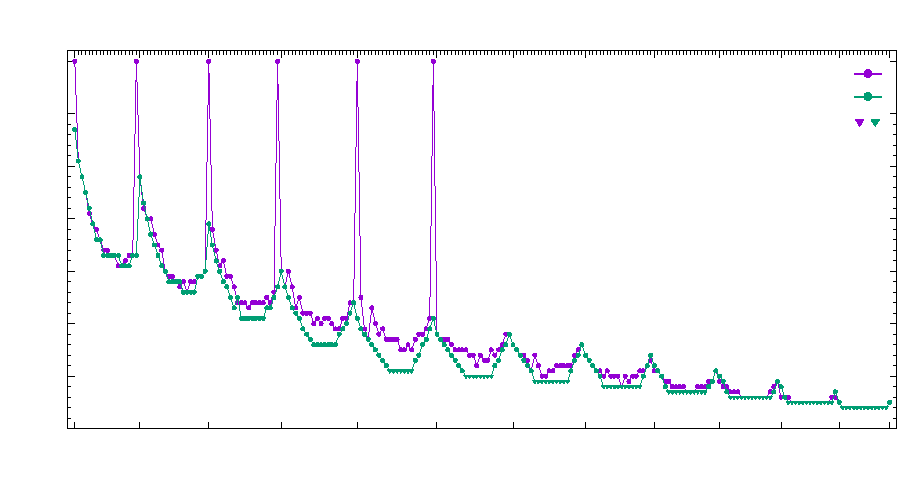
\includegraphics{resultados_5x5}}%
    \gplfronttext
  \end{picture}%
\endgroup
%
	\end{figure}
	}%
\end{frame}

\begin{frame}{Ejemplo ilustrativo en malla de $\mathsf{5\times 5}$}
	\vskip -7pt%
	\begin{figure}[H]
		\caption{Acomodo aleatorio inicial (izquierda) y acomodo encontrado por el algoritmo (derecha), mostrados en diferentes vistas.}%
		\arregloAntesDespues{caso=5x5, separacionAntesDespues=4, separacionVertical=0.33cm}{width=4.1cm}{width=2.8cm}%
	\end{figure}
\end{frame}


\begin{frame}{Mallas de $\mathsf{6\times 6}$}
	\vfill
	\Wider[1.85cm]{
	\begin{figure}[H]
		% GNUPLOT: LaTeX picture with Postscript
\begingroup
  % Encoding inside the plot.  In the header of your document, this encoding
  % should to defined, e.g., by using
  % \usepackage[latin1,<other encodings>]{inputenc}
  \inputencoding{latin1}%
  \makeatletter
  \providecommand\color[2][]{%
    \GenericError{(gnuplot) \space\space\space\@spaces}{%
      Package color not loaded in conjunction with
      terminal option `colourtext'%
    }{See the gnuplot documentation for explanation.%
    }{Either use 'blacktext' in gnuplot or load the package
      color.sty in LaTeX.}%
    \renewcommand\color[2][]{}%
  }%
  \providecommand\includegraphics[2][]{%
    \GenericError{(gnuplot) \space\space\space\@spaces}{%
      Package graphicx or graphics not loaded%
    }{See the gnuplot documentation for explanation.%
    }{The gnuplot epslatex terminal needs graphicx.sty or graphics.sty.}%
    \renewcommand\includegraphics[2][]{}%
  }%
  \providecommand\rotatebox[2]{#2}%
  \@ifundefined{ifGPcolor}{%
    \newif\ifGPcolor
    \GPcolortrue
  }{}%
  \@ifundefined{ifGPblacktext}{%
    \newif\ifGPblacktext
    \GPblacktexttrue
  }{}%
  % define a \g@addto@macro without @ in the name:
  \let\gplgaddtomacro\g@addto@macro
  % define empty templates for all commands taking text:
  \gdef\gplbacktext{}%
  \gdef\gplfronttext{}%
  \makeatother
  \ifGPblacktext
    % no textcolor at all
    \def\colorrgb#1{}%
    \def\colorgray#1{}%
  \else
    % gray or color?
    \ifGPcolor
      \def\colorrgb#1{\color[rgb]{#1}}%
      \def\colorgray#1{\color[gray]{#1}}%
      \expandafter\def\csname LTw\endcsname{\color{white}}%
      \expandafter\def\csname LTb\endcsname{\color{black}}%
      \expandafter\def\csname LTa\endcsname{\color{black}}%
      \expandafter\def\csname LT0\endcsname{\color[rgb]{1,0,0}}%
      \expandafter\def\csname LT1\endcsname{\color[rgb]{0,1,0}}%
      \expandafter\def\csname LT2\endcsname{\color[rgb]{0,0,1}}%
      \expandafter\def\csname LT3\endcsname{\color[rgb]{1,0,1}}%
      \expandafter\def\csname LT4\endcsname{\color[rgb]{0,1,1}}%
      \expandafter\def\csname LT5\endcsname{\color[rgb]{1,1,0}}%
      \expandafter\def\csname LT6\endcsname{\color[rgb]{0,0,0}}%
      \expandafter\def\csname LT7\endcsname{\color[rgb]{1,0.3,0}}%
      \expandafter\def\csname LT8\endcsname{\color[rgb]{0.5,0.5,0.5}}%
    \else
      % gray
      \def\colorrgb#1{\color{black}}%
      \def\colorgray#1{\color[gray]{#1}}%
      \expandafter\def\csname LTw\endcsname{\color{white}}%
      \expandafter\def\csname LTb\endcsname{\color{black}}%
      \expandafter\def\csname LTa\endcsname{\color{black}}%
      \expandafter\def\csname LT0\endcsname{\color{black}}%
      \expandafter\def\csname LT1\endcsname{\color{black}}%
      \expandafter\def\csname LT2\endcsname{\color{black}}%
      \expandafter\def\csname LT3\endcsname{\color{black}}%
      \expandafter\def\csname LT4\endcsname{\color{black}}%
      \expandafter\def\csname LT5\endcsname{\color{black}}%
      \expandafter\def\csname LT6\endcsname{\color{black}}%
      \expandafter\def\csname LT7\endcsname{\color{black}}%
      \expandafter\def\csname LT8\endcsname{\color{black}}%
    \fi
  \fi
    \setlength{\unitlength}{0.0500bp}%
    \ifx\gptboxheight\undefined%
      \newlength{\gptboxheight}%
      \newlength{\gptboxwidth}%
      \newsavebox{\gptboxtext}%
    \fi%
    \setlength{\fboxrule}{0.5pt}%
    \setlength{\fboxsep}{1pt}%
\begin{picture}(8466.00,4464.00)%
    \gplgaddtomacro\gplbacktext{%
      \csname LTb\endcsname%%
      \put(448,4000){\makebox(0,0)[r]{\strut{}\raisebox{2pt}{\fontsize{9}{9}\selectfont{$\infty$}}}}%
      \put(448,672){\makebox(0,0)[r]{\strut{}\fontsize{9}{9}\selectfont{20}}}%
      \put(448,1005){\makebox(0,0)[r]{\strut{}\fontsize{9}{9}\selectfont{30}}}%
      \put(448,1338){\makebox(0,0)[r]{\strut{}\fontsize{9}{9}\selectfont{40}}}%
      \put(448,1671){\makebox(0,0)[r]{\strut{}\fontsize{9}{9}\selectfont{50}}}%
      \put(448,2003){\makebox(0,0)[r]{\strut{}\fontsize{9}{9}\selectfont{60}}}%
      \put(448,2336){\makebox(0,0)[r]{\strut{}\fontsize{9}{9}\selectfont{70}}}%
      \put(448,2669){\makebox(0,0)[r]{\strut{}\fontsize{9}{9}\selectfont{80}}}%
      \put(448,3002){\makebox(0,0)[r]{\strut{}\fontsize{9}{9}\selectfont{90}}}%
      \put(448,3334){\makebox(0,0)[r]{\strut{}\fontsize{9}{9}\selectfont{100}}}%
      \put(448,3667){\makebox(0,0)[r]{\strut{}\fontsize{9}{9}\selectfont{110}}}%
      \put(525,396){\makebox(0,0){\strut{}\fontsize{8.0001}{8.0001}\selectfont{27,9}}}%
      \put(881,396){\makebox(0,0){\strut{}\fontsize{8.0001}{8.0001}\selectfont{27,8}}}%
      \put(1254,396){\makebox(0,0){\strut{}\fontsize{8.0001}{8.0001}\selectfont{27,7}}}%
      \put(1647,396){\makebox(0,0){\strut{}\fontsize{8.0001}{8.0001}\selectfont{27,6}}}%
      \put(2058,396){\makebox(0,0){\strut{}\fontsize{8.0001}{8.0001}\selectfont{27,5}}}%
      \put(2488,396){\makebox(0,0){\strut{}\fontsize{8.0001}{8.0001}\selectfont{27,4}}}%
      \put(2937,396){\makebox(0,0){\strut{}\fontsize{8.0001}{8.0001}\selectfont{27,3}}}%
      \put(3404,396){\makebox(0,0){\strut{}\fontsize{8.0001}{8.0001}\selectfont{27,2}}}%
      \put(3890,396){\makebox(0,0){\strut{}\fontsize{8.0001}{8.0001}\selectfont{27,1}}}%
      \put(4395,396){\makebox(0,0){\strut{}\fontsize{8.0001}{8.0001}\selectfont{27,0}}}%
      \put(4918,396){\makebox(0,0){\strut{}\fontsize{8.0001}{8.0001}\selectfont{26,0}}}%
      \put(5423,396){\makebox(0,0){\strut{}\fontsize{8.0001}{8.0001}\selectfont{25,0}}}%
      \put(5909,396){\makebox(0,0){\strut{}\fontsize{8.0001}{8.0001}\selectfont{24,0}}}%
      \put(6376,396){\makebox(0,0){\strut{}\fontsize{8.0001}{8.0001}\selectfont{23,0}}}%
      \put(6825,396){\makebox(0,0){\strut{}\fontsize{8.0001}{8.0001}\selectfont{22,0}}}%
      \put(7255,396){\makebox(0,0){\strut{}\fontsize{8.0001}{8.0001}\selectfont{21,0}}}%
      \put(7666,396){\makebox(0,0){\strut{}\fontsize{8.0001}{8.0001}\selectfont{20,0}}}%
      \put(8058,396){\makebox(0,0){\strut{}\fontsize{8.0001}{8.0001}\selectfont{19,0}}}%
      \put(8414,396){\makebox(0,0){\strut{}\fontsize{8.0001}{8.0001}\selectfont{0,19}}}%
      \put(473,4144){\rotatebox{90}{\makebox(0,0)[l]{\strut{}\fontsize{0.6}{0.6}\selectfont{26,10}}}}%
      \put(492,4144){\rotatebox{90}{\makebox(0,0)[l]{\strut{}\fontsize{0.6}{0.6}\selectfont{25,11}}}}%
      \put(510,4144){\rotatebox{90}{\makebox(0,0)[l]{\strut{}\fontsize{0.6}{0.6}\selectfont{24,12}}}}%
      \put(529,4144){\rotatebox{90}{\makebox(0,0)[l]{\strut{}\fontsize{0.6}{0.6}\selectfont{23,13}}}}%
      \put(548,4144){\rotatebox{90}{\makebox(0,0)[l]{\strut{}\fontsize{0.6}{0.6}\selectfont{22,14}}}}%
      \put(567,4144){\rotatebox{90}{\makebox(0,0)[l]{\strut{}\fontsize{0.6}{0.6}\selectfont{21,15}}}}%
      \put(585,4144){\rotatebox{90}{\makebox(0,0)[l]{\strut{}\fontsize{0.6}{0.6}\selectfont{20,16}}}}%
      \put(604,4144){\rotatebox{90}{\makebox(0,0)[l]{\strut{}\fontsize{0.6}{0.6}\selectfont{19,17}}}}%
      \put(623,4144){\rotatebox{90}{\makebox(0,0)[l]{\strut{}\fontsize{0.6}{0.6}\selectfont{18,18}}}}%
      \put(641,4144){\rotatebox{90}{\makebox(0,0)[l]{\strut{}\fontsize{0.6}{0.6}\selectfont{17,19}}}}%
      \put(660,4144){\rotatebox{90}{\makebox(0,0)[l]{\strut{}\fontsize{0.6}{0.6}\selectfont{16,20}}}}%
      \put(679,4144){\rotatebox{90}{\makebox(0,0)[l]{\strut{}\fontsize{0.6}{0.6}\selectfont{15,21}}}}%
      \put(697,4144){\rotatebox{90}{\makebox(0,0)[l]{\strut{}\fontsize{0.6}{0.6}\selectfont{14,22}}}}%
      \put(716,4144){\rotatebox{90}{\makebox(0,0)[l]{\strut{}\fontsize{0.6}{0.6}\selectfont{13,23}}}}%
      \put(735,4144){\rotatebox{90}{\makebox(0,0)[l]{\strut{}\fontsize{0.6}{0.6}\selectfont{12,24}}}}%
      \put(753,4144){\rotatebox{90}{\makebox(0,0)[l]{\strut{}\fontsize{0.6}{0.6}\selectfont{11,25}}}}%
      \put(772,4144){\rotatebox{90}{\makebox(0,0)[l]{\strut{}\fontsize{0.6}{0.6}\selectfont{10,26}}}}%
      \put(791,4144){\rotatebox{90}{\makebox(0,0)[l]{\strut{}\fontsize{0.6}{0.6}\selectfont{9,27}}}}%
      \put(828,4144){\rotatebox{90}{\makebox(0,0)[l]{\strut{}\fontsize{0.6}{0.6}\selectfont{26,9}}}}%
      \put(847,4144){\rotatebox{90}{\makebox(0,0)[l]{\strut{}\fontsize{0.6}{0.6}\selectfont{25,10}}}}%
      \put(866,4144){\rotatebox{90}{\makebox(0,0)[l]{\strut{}\fontsize{0.6}{0.6}\selectfont{24,11}}}}%
      \put(884,4144){\rotatebox{90}{\makebox(0,0)[l]{\strut{}\fontsize{0.6}{0.6}\selectfont{23,12}}}}%
      \put(903,4144){\rotatebox{90}{\makebox(0,0)[l]{\strut{}\fontsize{0.6}{0.6}\selectfont{22,13}}}}%
      \put(922,4144){\rotatebox{90}{\makebox(0,0)[l]{\strut{}\fontsize{0.6}{0.6}\selectfont{21,14}}}}%
      \put(940,4144){\rotatebox{90}{\makebox(0,0)[l]{\strut{}\fontsize{0.6}{0.6}\selectfont{20,15}}}}%
      \put(959,4144){\rotatebox{90}{\makebox(0,0)[l]{\strut{}\fontsize{0.6}{0.6}\selectfont{19,16}}}}%
      \put(978,4144){\rotatebox{90}{\makebox(0,0)[l]{\strut{}\fontsize{0.6}{0.6}\selectfont{18,17}}}}%
      \put(996,4144){\rotatebox{90}{\makebox(0,0)[l]{\strut{}\fontsize{0.6}{0.6}\selectfont{17,18}}}}%
      \put(1015,4144){\rotatebox{90}{\makebox(0,0)[l]{\strut{}\fontsize{0.6}{0.6}\selectfont{16,19}}}}%
      \put(1034,4144){\rotatebox{90}{\makebox(0,0)[l]{\strut{}\fontsize{0.6}{0.6}\selectfont{15,20}}}}%
      \put(1053,4144){\rotatebox{90}{\makebox(0,0)[l]{\strut{}\fontsize{0.6}{0.6}\selectfont{14,21}}}}%
      \put(1071,4144){\rotatebox{90}{\makebox(0,0)[l]{\strut{}\fontsize{0.6}{0.6}\selectfont{13,22}}}}%
      \put(1090,4144){\rotatebox{90}{\makebox(0,0)[l]{\strut{}\fontsize{0.6}{0.6}\selectfont{12,23}}}}%
      \put(1109,4144){\rotatebox{90}{\makebox(0,0)[l]{\strut{}\fontsize{0.6}{0.6}\selectfont{11,24}}}}%
      \put(1127,4144){\rotatebox{90}{\makebox(0,0)[l]{\strut{}\fontsize{0.6}{0.6}\selectfont{10,25}}}}%
      \put(1146,4144){\rotatebox{90}{\makebox(0,0)[l]{\strut{}\fontsize{0.6}{0.6}\selectfont{9,26}}}}%
      \put(1165,4144){\rotatebox{90}{\makebox(0,0)[l]{\strut{}\fontsize{0.6}{0.6}\selectfont{8,27}}}}%
      \put(1202,4144){\rotatebox{90}{\makebox(0,0)[l]{\strut{}\fontsize{0.6}{0.6}\selectfont{26,8}}}}%
      \put(1221,4144){\rotatebox{90}{\makebox(0,0)[l]{\strut{}\fontsize{0.6}{0.6}\selectfont{25,9}}}}%
      \put(1239,4144){\rotatebox{90}{\makebox(0,0)[l]{\strut{}\fontsize{0.6}{0.6}\selectfont{24,10}}}}%
      \put(1258,4144){\rotatebox{90}{\makebox(0,0)[l]{\strut{}\fontsize{0.6}{0.6}\selectfont{23,11}}}}%
      \put(1277,4144){\rotatebox{90}{\makebox(0,0)[l]{\strut{}\fontsize{0.6}{0.6}\selectfont{22,12}}}}%
      \put(1296,4144){\rotatebox{90}{\makebox(0,0)[l]{\strut{}\fontsize{0.6}{0.6}\selectfont{21,13}}}}%
      \put(1314,4144){\rotatebox{90}{\makebox(0,0)[l]{\strut{}\fontsize{0.6}{0.6}\selectfont{20,14}}}}%
      \put(1333,4144){\rotatebox{90}{\makebox(0,0)[l]{\strut{}\fontsize{0.6}{0.6}\selectfont{19,15}}}}%
      \put(1352,4144){\rotatebox{90}{\makebox(0,0)[l]{\strut{}\fontsize{0.6}{0.6}\selectfont{18,16}}}}%
      \put(1370,4144){\rotatebox{90}{\makebox(0,0)[l]{\strut{}\fontsize{0.6}{0.6}\selectfont{17,17}}}}%
      \put(1389,4144){\rotatebox{90}{\makebox(0,0)[l]{\strut{}\fontsize{0.6}{0.6}\selectfont{16,18}}}}%
      \put(1408,4144){\rotatebox{90}{\makebox(0,0)[l]{\strut{}\fontsize{0.6}{0.6}\selectfont{15,19}}}}%
      \put(1426,4144){\rotatebox{90}{\makebox(0,0)[l]{\strut{}\fontsize{0.6}{0.6}\selectfont{14,20}}}}%
      \put(1445,4144){\rotatebox{90}{\makebox(0,0)[l]{\strut{}\fontsize{0.6}{0.6}\selectfont{13,21}}}}%
      \put(1464,4144){\rotatebox{90}{\makebox(0,0)[l]{\strut{}\fontsize{0.6}{0.6}\selectfont{12,22}}}}%
      \put(1482,4144){\rotatebox{90}{\makebox(0,0)[l]{\strut{}\fontsize{0.6}{0.6}\selectfont{11,23}}}}%
      \put(1501,4144){\rotatebox{90}{\makebox(0,0)[l]{\strut{}\fontsize{0.6}{0.6}\selectfont{10,24}}}}%
      \put(1520,4144){\rotatebox{90}{\makebox(0,0)[l]{\strut{}\fontsize{0.6}{0.6}\selectfont{9,25}}}}%
      \put(1539,4144){\rotatebox{90}{\makebox(0,0)[l]{\strut{}\fontsize{0.6}{0.6}\selectfont{8,26}}}}%
      \put(1557,4144){\rotatebox{90}{\makebox(0,0)[l]{\strut{}\fontsize{0.6}{0.6}\selectfont{7,27}}}}%
      \put(1595,4144){\rotatebox{90}{\makebox(0,0)[l]{\strut{}\fontsize{0.6}{0.6}\selectfont{26,7}}}}%
      \put(1613,4144){\rotatebox{90}{\makebox(0,0)[l]{\strut{}\fontsize{0.6}{0.6}\selectfont{25,8}}}}%
      \put(1632,4144){\rotatebox{90}{\makebox(0,0)[l]{\strut{}\fontsize{0.6}{0.6}\selectfont{24,9}}}}%
      \put(1651,4144){\rotatebox{90}{\makebox(0,0)[l]{\strut{}\fontsize{0.6}{0.6}\selectfont{23,10}}}}%
      \put(1669,4144){\rotatebox{90}{\makebox(0,0)[l]{\strut{}\fontsize{0.6}{0.6}\selectfont{22,11}}}}%
      \put(1688,4144){\rotatebox{90}{\makebox(0,0)[l]{\strut{}\fontsize{0.6}{0.6}\selectfont{21,12}}}}%
      \put(1707,4144){\rotatebox{90}{\makebox(0,0)[l]{\strut{}\fontsize{0.6}{0.6}\selectfont{20,13}}}}%
      \put(1725,4144){\rotatebox{90}{\makebox(0,0)[l]{\strut{}\fontsize{0.6}{0.6}\selectfont{19,14}}}}%
      \put(1744,4144){\rotatebox{90}{\makebox(0,0)[l]{\strut{}\fontsize{0.6}{0.6}\selectfont{18,15}}}}%
      \put(1763,4144){\rotatebox{90}{\makebox(0,0)[l]{\strut{}\fontsize{0.6}{0.6}\selectfont{17,16}}}}%
      \put(1782,4144){\rotatebox{90}{\makebox(0,0)[l]{\strut{}\fontsize{0.6}{0.6}\selectfont{16,17}}}}%
      \put(1800,4144){\rotatebox{90}{\makebox(0,0)[l]{\strut{}\fontsize{0.6}{0.6}\selectfont{15,18}}}}%
      \put(1819,4144){\rotatebox{90}{\makebox(0,0)[l]{\strut{}\fontsize{0.6}{0.6}\selectfont{14,19}}}}%
      \put(1838,4144){\rotatebox{90}{\makebox(0,0)[l]{\strut{}\fontsize{0.6}{0.6}\selectfont{13,20}}}}%
      \put(1856,4144){\rotatebox{90}{\makebox(0,0)[l]{\strut{}\fontsize{0.6}{0.6}\selectfont{12,21}}}}%
      \put(1875,4144){\rotatebox{90}{\makebox(0,0)[l]{\strut{}\fontsize{0.6}{0.6}\selectfont{11,22}}}}%
      \put(1894,4144){\rotatebox{90}{\makebox(0,0)[l]{\strut{}\fontsize{0.6}{0.6}\selectfont{10,23}}}}%
      \put(1912,4144){\rotatebox{90}{\makebox(0,0)[l]{\strut{}\fontsize{0.6}{0.6}\selectfont{9,24}}}}%
      \put(1931,4144){\rotatebox{90}{\makebox(0,0)[l]{\strut{}\fontsize{0.6}{0.6}\selectfont{8,25}}}}%
      \put(1950,4144){\rotatebox{90}{\makebox(0,0)[l]{\strut{}\fontsize{0.6}{0.6}\selectfont{7,26}}}}%
      \put(1968,4144){\rotatebox{90}{\makebox(0,0)[l]{\strut{}\fontsize{0.6}{0.6}\selectfont{6,27}}}}%
      \put(2006,4144){\rotatebox{90}{\makebox(0,0)[l]{\strut{}\fontsize{0.6}{0.6}\selectfont{26,6}}}}%
      \put(2025,4144){\rotatebox{90}{\makebox(0,0)[l]{\strut{}\fontsize{0.6}{0.6}\selectfont{25,7}}}}%
      \put(2043,4144){\rotatebox{90}{\makebox(0,0)[l]{\strut{}\fontsize{0.6}{0.6}\selectfont{24,8}}}}%
      \put(2062,4144){\rotatebox{90}{\makebox(0,0)[l]{\strut{}\fontsize{0.6}{0.6}\selectfont{23,9}}}}%
      \put(2081,4144){\rotatebox{90}{\makebox(0,0)[l]{\strut{}\fontsize{0.6}{0.6}\selectfont{22,10}}}}%
      \put(2099,4144){\rotatebox{90}{\makebox(0,0)[l]{\strut{}\fontsize{0.6}{0.6}\selectfont{21,11}}}}%
      \put(2118,4144){\rotatebox{90}{\makebox(0,0)[l]{\strut{}\fontsize{0.6}{0.6}\selectfont{20,12}}}}%
      \put(2137,4144){\rotatebox{90}{\makebox(0,0)[l]{\strut{}\fontsize{0.6}{0.6}\selectfont{19,13}}}}%
      \put(2155,4144){\rotatebox{90}{\makebox(0,0)[l]{\strut{}\fontsize{0.6}{0.6}\selectfont{18,14}}}}%
      \put(2174,4144){\rotatebox{90}{\makebox(0,0)[l]{\strut{}\fontsize{0.6}{0.6}\selectfont{17,15}}}}%
      \put(2193,4144){\rotatebox{90}{\makebox(0,0)[l]{\strut{}\fontsize{0.6}{0.6}\selectfont{16,16}}}}%
      \put(2211,4144){\rotatebox{90}{\makebox(0,0)[l]{\strut{}\fontsize{0.6}{0.6}\selectfont{15,17}}}}%
      \put(2230,4144){\rotatebox{90}{\makebox(0,0)[l]{\strut{}\fontsize{0.6}{0.6}\selectfont{14,18}}}}%
      \put(2249,4144){\rotatebox{90}{\makebox(0,0)[l]{\strut{}\fontsize{0.6}{0.6}\selectfont{13,19}}}}%
      \put(2268,4144){\rotatebox{90}{\makebox(0,0)[l]{\strut{}\fontsize{0.6}{0.6}\selectfont{12,20}}}}%
      \put(2286,4144){\rotatebox{90}{\makebox(0,0)[l]{\strut{}\fontsize{0.6}{0.6}\selectfont{11,21}}}}%
      \put(2305,4144){\rotatebox{90}{\makebox(0,0)[l]{\strut{}\fontsize{0.6}{0.6}\selectfont{10,22}}}}%
      \put(2324,4144){\rotatebox{90}{\makebox(0,0)[l]{\strut{}\fontsize{0.6}{0.6}\selectfont{9,23}}}}%
      \put(2342,4144){\rotatebox{90}{\makebox(0,0)[l]{\strut{}\fontsize{0.6}{0.6}\selectfont{8,24}}}}%
      \put(2361,4144){\rotatebox{90}{\makebox(0,0)[l]{\strut{}\fontsize{0.6}{0.6}\selectfont{7,25}}}}%
      \put(2380,4144){\rotatebox{90}{\makebox(0,0)[l]{\strut{}\fontsize{0.6}{0.6}\selectfont{6,26}}}}%
      \put(2398,4144){\rotatebox{90}{\makebox(0,0)[l]{\strut{}\fontsize{0.6}{0.6}\selectfont{5,27}}}}%
      \put(2436,4144){\rotatebox{90}{\makebox(0,0)[l]{\strut{}\fontsize{0.6}{0.6}\selectfont{26,5}}}}%
      \put(2454,4144){\rotatebox{90}{\makebox(0,0)[l]{\strut{}\fontsize{0.6}{0.6}\selectfont{25,6}}}}%
      \put(2473,4144){\rotatebox{90}{\makebox(0,0)[l]{\strut{}\fontsize{0.6}{0.6}\selectfont{24,7}}}}%
      \put(2492,4144){\rotatebox{90}{\makebox(0,0)[l]{\strut{}\fontsize{0.6}{0.6}\selectfont{23,8}}}}%
      \put(2511,4144){\rotatebox{90}{\makebox(0,0)[l]{\strut{}\fontsize{0.6}{0.6}\selectfont{22,9}}}}%
      \put(2529,4144){\rotatebox{90}{\makebox(0,0)[l]{\strut{}\fontsize{0.6}{0.6}\selectfont{21,10}}}}%
      \put(2548,4144){\rotatebox{90}{\makebox(0,0)[l]{\strut{}\fontsize{0.6}{0.6}\selectfont{20,11}}}}%
      \put(2567,4144){\rotatebox{90}{\makebox(0,0)[l]{\strut{}\fontsize{0.6}{0.6}\selectfont{19,12}}}}%
      \put(2585,4144){\rotatebox{90}{\makebox(0,0)[l]{\strut{}\fontsize{0.6}{0.6}\selectfont{18,13}}}}%
      \put(2604,4144){\rotatebox{90}{\makebox(0,0)[l]{\strut{}\fontsize{0.6}{0.6}\selectfont{17,14}}}}%
      \put(2623,4144){\rotatebox{90}{\makebox(0,0)[l]{\strut{}\fontsize{0.6}{0.6}\selectfont{16,15}}}}%
      \put(2641,4144){\rotatebox{90}{\makebox(0,0)[l]{\strut{}\fontsize{0.6}{0.6}\selectfont{15,16}}}}%
      \put(2660,4144){\rotatebox{90}{\makebox(0,0)[l]{\strut{}\fontsize{0.6}{0.6}\selectfont{14,17}}}}%
      \put(2679,4144){\rotatebox{90}{\makebox(0,0)[l]{\strut{}\fontsize{0.6}{0.6}\selectfont{13,18}}}}%
      \put(2697,4144){\rotatebox{90}{\makebox(0,0)[l]{\strut{}\fontsize{0.6}{0.6}\selectfont{12,19}}}}%
      \put(2716,4144){\rotatebox{90}{\makebox(0,0)[l]{\strut{}\fontsize{0.6}{0.6}\selectfont{11,20}}}}%
      \put(2735,4144){\rotatebox{90}{\makebox(0,0)[l]{\strut{}\fontsize{0.6}{0.6}\selectfont{10,21}}}}%
      \put(2754,4144){\rotatebox{90}{\makebox(0,0)[l]{\strut{}\fontsize{0.6}{0.6}\selectfont{9,22}}}}%
      \put(2772,4144){\rotatebox{90}{\makebox(0,0)[l]{\strut{}\fontsize{0.6}{0.6}\selectfont{8,23}}}}%
      \put(2791,4144){\rotatebox{90}{\makebox(0,0)[l]{\strut{}\fontsize{0.6}{0.6}\selectfont{7,24}}}}%
      \put(2810,4144){\rotatebox{90}{\makebox(0,0)[l]{\strut{}\fontsize{0.6}{0.6}\selectfont{6,25}}}}%
      \put(2828,4144){\rotatebox{90}{\makebox(0,0)[l]{\strut{}\fontsize{0.6}{0.6}\selectfont{5,26}}}}%
      \put(2847,4144){\rotatebox{90}{\makebox(0,0)[l]{\strut{}\fontsize{0.6}{0.6}\selectfont{4,27}}}}%
      \put(2884,4144){\rotatebox{90}{\makebox(0,0)[l]{\strut{}\fontsize{0.6}{0.6}\selectfont{26,4}}}}%
      \put(2903,4144){\rotatebox{90}{\makebox(0,0)[l]{\strut{}\fontsize{0.6}{0.6}\selectfont{25,5}}}}%
      \put(2922,4144){\rotatebox{90}{\makebox(0,0)[l]{\strut{}\fontsize{0.6}{0.6}\selectfont{24,6}}}}%
      \put(2940,4144){\rotatebox{90}{\makebox(0,0)[l]{\strut{}\fontsize{0.6}{0.6}\selectfont{23,7}}}}%
      \put(2959,4144){\rotatebox{90}{\makebox(0,0)[l]{\strut{}\fontsize{0.6}{0.6}\selectfont{22,8}}}}%
      \put(2978,4144){\rotatebox{90}{\makebox(0,0)[l]{\strut{}\fontsize{0.6}{0.6}\selectfont{21,9}}}}%
      \put(2997,4144){\rotatebox{90}{\makebox(0,0)[l]{\strut{}\fontsize{0.6}{0.6}\selectfont{20,10}}}}%
      \put(3015,4144){\rotatebox{90}{\makebox(0,0)[l]{\strut{}\fontsize{0.6}{0.6}\selectfont{19,11}}}}%
      \put(3034,4144){\rotatebox{90}{\makebox(0,0)[l]{\strut{}\fontsize{0.6}{0.6}\selectfont{18,12}}}}%
      \put(3053,4144){\rotatebox{90}{\makebox(0,0)[l]{\strut{}\fontsize{0.6}{0.6}\selectfont{17,13}}}}%
      \put(3071,4144){\rotatebox{90}{\makebox(0,0)[l]{\strut{}\fontsize{0.6}{0.6}\selectfont{16,14}}}}%
      \put(3090,4144){\rotatebox{90}{\makebox(0,0)[l]{\strut{}\fontsize{0.6}{0.6}\selectfont{15,15}}}}%
      \put(3109,4144){\rotatebox{90}{\makebox(0,0)[l]{\strut{}\fontsize{0.6}{0.6}\selectfont{14,16}}}}%
      \put(3127,4144){\rotatebox{90}{\makebox(0,0)[l]{\strut{}\fontsize{0.6}{0.6}\selectfont{13,17}}}}%
      \put(3146,4144){\rotatebox{90}{\makebox(0,0)[l]{\strut{}\fontsize{0.6}{0.6}\selectfont{12,18}}}}%
      \put(3165,4144){\rotatebox{90}{\makebox(0,0)[l]{\strut{}\fontsize{0.6}{0.6}\selectfont{11,19}}}}%
      \put(3183,4144){\rotatebox{90}{\makebox(0,0)[l]{\strut{}\fontsize{0.6}{0.6}\selectfont{10,20}}}}%
      \put(3202,4144){\rotatebox{90}{\makebox(0,0)[l]{\strut{}\fontsize{0.6}{0.6}\selectfont{9,21}}}}%
      \put(3221,4144){\rotatebox{90}{\makebox(0,0)[l]{\strut{}\fontsize{0.6}{0.6}\selectfont{8,22}}}}%
      \put(3240,4144){\rotatebox{90}{\makebox(0,0)[l]{\strut{}\fontsize{0.6}{0.6}\selectfont{7,23}}}}%
      \put(3258,4144){\rotatebox{90}{\makebox(0,0)[l]{\strut{}\fontsize{0.6}{0.6}\selectfont{6,24}}}}%
      \put(3277,4144){\rotatebox{90}{\makebox(0,0)[l]{\strut{}\fontsize{0.6}{0.6}\selectfont{5,25}}}}%
      \put(3296,4144){\rotatebox{90}{\makebox(0,0)[l]{\strut{}\fontsize{0.6}{0.6}\selectfont{4,26}}}}%
      \put(3314,4144){\rotatebox{90}{\makebox(0,0)[l]{\strut{}\fontsize{0.6}{0.6}\selectfont{3,27}}}}%
      \put(3352,4144){\rotatebox{90}{\makebox(0,0)[l]{\strut{}\fontsize{0.6}{0.6}\selectfont{26,3}}}}%
      \put(3370,4144){\rotatebox{90}{\makebox(0,0)[l]{\strut{}\fontsize{0.6}{0.6}\selectfont{25,4}}}}%
      \put(3389,4144){\rotatebox{90}{\makebox(0,0)[l]{\strut{}\fontsize{0.6}{0.6}\selectfont{24,5}}}}%
      \put(3408,4144){\rotatebox{90}{\makebox(0,0)[l]{\strut{}\fontsize{0.6}{0.6}\selectfont{23,6}}}}%
      \put(3426,4144){\rotatebox{90}{\makebox(0,0)[l]{\strut{}\fontsize{0.6}{0.6}\selectfont{22,7}}}}%
      \put(3445,4144){\rotatebox{90}{\makebox(0,0)[l]{\strut{}\fontsize{0.6}{0.6}\selectfont{21,8}}}}%
      \put(3464,4144){\rotatebox{90}{\makebox(0,0)[l]{\strut{}\fontsize{0.6}{0.6}\selectfont{20,9}}}}%
      \put(3483,4144){\rotatebox{90}{\makebox(0,0)[l]{\strut{}\fontsize{0.6}{0.6}\selectfont{19,10}}}}%
      \put(3501,4144){\rotatebox{90}{\makebox(0,0)[l]{\strut{}\fontsize{0.6}{0.6}\selectfont{18,11}}}}%
      \put(3520,4144){\rotatebox{90}{\makebox(0,0)[l]{\strut{}\fontsize{0.6}{0.6}\selectfont{17,12}}}}%
      \put(3539,4144){\rotatebox{90}{\makebox(0,0)[l]{\strut{}\fontsize{0.6}{0.6}\selectfont{16,13}}}}%
      \put(3557,4144){\rotatebox{90}{\makebox(0,0)[l]{\strut{}\fontsize{0.6}{0.6}\selectfont{15,14}}}}%
      \put(3576,4144){\rotatebox{90}{\makebox(0,0)[l]{\strut{}\fontsize{0.6}{0.6}\selectfont{14,15}}}}%
      \put(3595,4144){\rotatebox{90}{\makebox(0,0)[l]{\strut{}\fontsize{0.6}{0.6}\selectfont{13,16}}}}%
      \put(3613,4144){\rotatebox{90}{\makebox(0,0)[l]{\strut{}\fontsize{0.6}{0.6}\selectfont{12,17}}}}%
      \put(3632,4144){\rotatebox{90}{\makebox(0,0)[l]{\strut{}\fontsize{0.6}{0.6}\selectfont{11,18}}}}%
      \put(3651,4144){\rotatebox{90}{\makebox(0,0)[l]{\strut{}\fontsize{0.6}{0.6}\selectfont{10,19}}}}%
      \put(3669,4144){\rotatebox{90}{\makebox(0,0)[l]{\strut{}\fontsize{0.6}{0.6}\selectfont{9,20}}}}%
      \put(3688,4144){\rotatebox{90}{\makebox(0,0)[l]{\strut{}\fontsize{0.6}{0.6}\selectfont{8,21}}}}%
      \put(3707,4144){\rotatebox{90}{\makebox(0,0)[l]{\strut{}\fontsize{0.6}{0.6}\selectfont{7,22}}}}%
      \put(3726,4144){\rotatebox{90}{\makebox(0,0)[l]{\strut{}\fontsize{0.6}{0.6}\selectfont{6,23}}}}%
      \put(3744,4144){\rotatebox{90}{\makebox(0,0)[l]{\strut{}\fontsize{0.6}{0.6}\selectfont{5,24}}}}%
      \put(3763,4144){\rotatebox{90}{\makebox(0,0)[l]{\strut{}\fontsize{0.6}{0.6}\selectfont{4,25}}}}%
      \put(3782,4144){\rotatebox{90}{\makebox(0,0)[l]{\strut{}\fontsize{0.6}{0.6}\selectfont{3,26}}}}%
      \put(3800,4144){\rotatebox{90}{\makebox(0,0)[l]{\strut{}\fontsize{0.6}{0.6}\selectfont{2,27}}}}%
      \put(3838,4144){\rotatebox{90}{\makebox(0,0)[l]{\strut{}\fontsize{0.6}{0.6}\selectfont{26,2}}}}%
      \put(3856,4144){\rotatebox{90}{\makebox(0,0)[l]{\strut{}\fontsize{0.6}{0.6}\selectfont{25,3}}}}%
      \put(3875,4144){\rotatebox{90}{\makebox(0,0)[l]{\strut{}\fontsize{0.6}{0.6}\selectfont{24,4}}}}%
      \put(3894,4144){\rotatebox{90}{\makebox(0,0)[l]{\strut{}\fontsize{0.6}{0.6}\selectfont{23,5}}}}%
      \put(3912,4144){\rotatebox{90}{\makebox(0,0)[l]{\strut{}\fontsize{0.6}{0.6}\selectfont{22,6}}}}%
      \put(3931,4144){\rotatebox{90}{\makebox(0,0)[l]{\strut{}\fontsize{0.6}{0.6}\selectfont{21,7}}}}%
      \put(3950,4144){\rotatebox{90}{\makebox(0,0)[l]{\strut{}\fontsize{0.6}{0.6}\selectfont{20,8}}}}%
      \put(3969,4144){\rotatebox{90}{\makebox(0,0)[l]{\strut{}\fontsize{0.6}{0.6}\selectfont{19,9}}}}%
      \put(3987,4144){\rotatebox{90}{\makebox(0,0)[l]{\strut{}\fontsize{0.6}{0.6}\selectfont{18,10}}}}%
      \put(4006,4144){\rotatebox{90}{\makebox(0,0)[l]{\strut{}\fontsize{0.6}{0.6}\selectfont{17,11}}}}%
      \put(4025,4144){\rotatebox{90}{\makebox(0,0)[l]{\strut{}\fontsize{0.6}{0.6}\selectfont{16,12}}}}%
      \put(4043,4144){\rotatebox{90}{\makebox(0,0)[l]{\strut{}\fontsize{0.6}{0.6}\selectfont{15,13}}}}%
      \put(4062,4144){\rotatebox{90}{\makebox(0,0)[l]{\strut{}\fontsize{0.6}{0.6}\selectfont{14,14}}}}%
      \put(4081,4144){\rotatebox{90}{\makebox(0,0)[l]{\strut{}\fontsize{0.6}{0.6}\selectfont{13,15}}}}%
      \put(4099,4144){\rotatebox{90}{\makebox(0,0)[l]{\strut{}\fontsize{0.6}{0.6}\selectfont{12,16}}}}%
      \put(4118,4144){\rotatebox{90}{\makebox(0,0)[l]{\strut{}\fontsize{0.6}{0.6}\selectfont{11,17}}}}%
      \put(4137,4144){\rotatebox{90}{\makebox(0,0)[l]{\strut{}\fontsize{0.6}{0.6}\selectfont{10,18}}}}%
      \put(4155,4144){\rotatebox{90}{\makebox(0,0)[l]{\strut{}\fontsize{0.6}{0.6}\selectfont{9,19}}}}%
      \put(4174,4144){\rotatebox{90}{\makebox(0,0)[l]{\strut{}\fontsize{0.6}{0.6}\selectfont{8,20}}}}%
      \put(4193,4144){\rotatebox{90}{\makebox(0,0)[l]{\strut{}\fontsize{0.6}{0.6}\selectfont{7,21}}}}%
      \put(4212,4144){\rotatebox{90}{\makebox(0,0)[l]{\strut{}\fontsize{0.6}{0.6}\selectfont{6,22}}}}%
      \put(4230,4144){\rotatebox{90}{\makebox(0,0)[l]{\strut{}\fontsize{0.6}{0.6}\selectfont{5,23}}}}%
      \put(4249,4144){\rotatebox{90}{\makebox(0,0)[l]{\strut{}\fontsize{0.6}{0.6}\selectfont{4,24}}}}%
      \put(4268,4144){\rotatebox{90}{\makebox(0,0)[l]{\strut{}\fontsize{0.6}{0.6}\selectfont{3,25}}}}%
      \put(4286,4144){\rotatebox{90}{\makebox(0,0)[l]{\strut{}\fontsize{0.6}{0.6}\selectfont{2,26}}}}%
      \put(4305,4144){\rotatebox{90}{\makebox(0,0)[l]{\strut{}\fontsize{0.6}{0.6}\selectfont{1,27}}}}%
      \put(4342,4144){\rotatebox{90}{\makebox(0,0)[l]{\strut{}\fontsize{0.6}{0.6}\selectfont{26,1}}}}%
      \put(4361,4144){\rotatebox{90}{\makebox(0,0)[l]{\strut{}\fontsize{0.6}{0.6}\selectfont{25,2}}}}%
      \put(4380,4144){\rotatebox{90}{\makebox(0,0)[l]{\strut{}\fontsize{0.6}{0.6}\selectfont{24,3}}}}%
      \put(4399,4144){\rotatebox{90}{\makebox(0,0)[l]{\strut{}\fontsize{0.6}{0.6}\selectfont{23,4}}}}%
      \put(4417,4144){\rotatebox{90}{\makebox(0,0)[l]{\strut{}\fontsize{0.6}{0.6}\selectfont{22,5}}}}%
      \put(4436,4144){\rotatebox{90}{\makebox(0,0)[l]{\strut{}\fontsize{0.6}{0.6}\selectfont{21,6}}}}%
      \put(4455,4144){\rotatebox{90}{\makebox(0,0)[l]{\strut{}\fontsize{0.6}{0.6}\selectfont{20,7}}}}%
      \put(4473,4144){\rotatebox{90}{\makebox(0,0)[l]{\strut{}\fontsize{0.6}{0.6}\selectfont{19,8}}}}%
      \put(4492,4144){\rotatebox{90}{\makebox(0,0)[l]{\strut{}\fontsize{0.6}{0.6}\selectfont{18,9}}}}%
      \put(4511,4144){\rotatebox{90}{\makebox(0,0)[l]{\strut{}\fontsize{0.6}{0.6}\selectfont{17,10}}}}%
      \put(4529,4144){\rotatebox{90}{\makebox(0,0)[l]{\strut{}\fontsize{0.6}{0.6}\selectfont{16,11}}}}%
      \put(4548,4144){\rotatebox{90}{\makebox(0,0)[l]{\strut{}\fontsize{0.6}{0.6}\selectfont{15,12}}}}%
      \put(4567,4144){\rotatebox{90}{\makebox(0,0)[l]{\strut{}\fontsize{0.6}{0.6}\selectfont{14,13}}}}%
      \put(4585,4144){\rotatebox{90}{\makebox(0,0)[l]{\strut{}\fontsize{0.6}{0.6}\selectfont{13,14}}}}%
      \put(4604,4144){\rotatebox{90}{\makebox(0,0)[l]{\strut{}\fontsize{0.6}{0.6}\selectfont{12,15}}}}%
      \put(4623,4144){\rotatebox{90}{\makebox(0,0)[l]{\strut{}\fontsize{0.6}{0.6}\selectfont{11,16}}}}%
      \put(4642,4144){\rotatebox{90}{\makebox(0,0)[l]{\strut{}\fontsize{0.6}{0.6}\selectfont{10,17}}}}%
      \put(4660,4144){\rotatebox{90}{\makebox(0,0)[l]{\strut{}\fontsize{0.6}{0.6}\selectfont{9,18}}}}%
      \put(4679,4144){\rotatebox{90}{\makebox(0,0)[l]{\strut{}\fontsize{0.6}{0.6}\selectfont{8,19}}}}%
      \put(4698,4144){\rotatebox{90}{\makebox(0,0)[l]{\strut{}\fontsize{0.6}{0.6}\selectfont{7,20}}}}%
      \put(4716,4144){\rotatebox{90}{\makebox(0,0)[l]{\strut{}\fontsize{0.6}{0.6}\selectfont{6,21}}}}%
      \put(4735,4144){\rotatebox{90}{\makebox(0,0)[l]{\strut{}\fontsize{0.6}{0.6}\selectfont{5,22}}}}%
      \put(4754,4144){\rotatebox{90}{\makebox(0,0)[l]{\strut{}\fontsize{0.6}{0.6}\selectfont{4,23}}}}%
      \put(4772,4144){\rotatebox{90}{\makebox(0,0)[l]{\strut{}\fontsize{0.6}{0.6}\selectfont{3,24}}}}%
      \put(4791,4144){\rotatebox{90}{\makebox(0,0)[l]{\strut{}\fontsize{0.6}{0.6}\selectfont{2,25}}}}%
      \put(4810,4144){\rotatebox{90}{\makebox(0,0)[l]{\strut{}\fontsize{0.6}{0.6}\selectfont{1,26}}}}%
      \put(4828,4144){\rotatebox{90}{\makebox(0,0)[l]{\strut{}\fontsize{0.6}{0.6}\selectfont{0,27}}}}%
      \put(4866,4144){\rotatebox{90}{\makebox(0,0)[l]{\strut{}\fontsize{0.6}{0.6}\selectfont{25,1}}}}%
      \put(4885,4144){\rotatebox{90}{\makebox(0,0)[l]{\strut{}\fontsize{0.6}{0.6}\selectfont{24,2}}}}%
      \put(4903,4144){\rotatebox{90}{\makebox(0,0)[l]{\strut{}\fontsize{0.6}{0.6}\selectfont{23,3}}}}%
      \put(4922,4144){\rotatebox{90}{\makebox(0,0)[l]{\strut{}\fontsize{0.6}{0.6}\selectfont{22,4}}}}%
      \put(4941,4144){\rotatebox{90}{\makebox(0,0)[l]{\strut{}\fontsize{0.6}{0.6}\selectfont{21,5}}}}%
      \put(4959,4144){\rotatebox{90}{\makebox(0,0)[l]{\strut{}\fontsize{0.6}{0.6}\selectfont{20,6}}}}%
      \put(4978,4144){\rotatebox{90}{\makebox(0,0)[l]{\strut{}\fontsize{0.6}{0.6}\selectfont{19,7}}}}%
      \put(4997,4144){\rotatebox{90}{\makebox(0,0)[l]{\strut{}\fontsize{0.6}{0.6}\selectfont{18,8}}}}%
      \put(5015,4144){\rotatebox{90}{\makebox(0,0)[l]{\strut{}\fontsize{0.6}{0.6}\selectfont{17,9}}}}%
      \put(5034,4144){\rotatebox{90}{\makebox(0,0)[l]{\strut{}\fontsize{0.6}{0.6}\selectfont{16,10}}}}%
      \put(5053,4144){\rotatebox{90}{\makebox(0,0)[l]{\strut{}\fontsize{0.6}{0.6}\selectfont{15,11}}}}%
      \put(5071,4144){\rotatebox{90}{\makebox(0,0)[l]{\strut{}\fontsize{0.6}{0.6}\selectfont{14,12}}}}%
      \put(5090,4144){\rotatebox{90}{\makebox(0,0)[l]{\strut{}\fontsize{0.6}{0.6}\selectfont{13,13}}}}%
      \put(5109,4144){\rotatebox{90}{\makebox(0,0)[l]{\strut{}\fontsize{0.6}{0.6}\selectfont{12,14}}}}%
      \put(5128,4144){\rotatebox{90}{\makebox(0,0)[l]{\strut{}\fontsize{0.6}{0.6}\selectfont{11,15}}}}%
      \put(5146,4144){\rotatebox{90}{\makebox(0,0)[l]{\strut{}\fontsize{0.6}{0.6}\selectfont{10,16}}}}%
      \put(5165,4144){\rotatebox{90}{\makebox(0,0)[l]{\strut{}\fontsize{0.6}{0.6}\selectfont{9,17}}}}%
      \put(5184,4144){\rotatebox{90}{\makebox(0,0)[l]{\strut{}\fontsize{0.6}{0.6}\selectfont{8,18}}}}%
      \put(5202,4144){\rotatebox{90}{\makebox(0,0)[l]{\strut{}\fontsize{0.6}{0.6}\selectfont{7,19}}}}%
      \put(5221,4144){\rotatebox{90}{\makebox(0,0)[l]{\strut{}\fontsize{0.6}{0.6}\selectfont{6,20}}}}%
      \put(5240,4144){\rotatebox{90}{\makebox(0,0)[l]{\strut{}\fontsize{0.6}{0.6}\selectfont{5,21}}}}%
      \put(5258,4144){\rotatebox{90}{\makebox(0,0)[l]{\strut{}\fontsize{0.6}{0.6}\selectfont{4,22}}}}%
      \put(5277,4144){\rotatebox{90}{\makebox(0,0)[l]{\strut{}\fontsize{0.6}{0.6}\selectfont{3,23}}}}%
      \put(5296,4144){\rotatebox{90}{\makebox(0,0)[l]{\strut{}\fontsize{0.6}{0.6}\selectfont{2,24}}}}%
      \put(5314,4144){\rotatebox{90}{\makebox(0,0)[l]{\strut{}\fontsize{0.6}{0.6}\selectfont{1,25}}}}%
      \put(5333,4144){\rotatebox{90}{\makebox(0,0)[l]{\strut{}\fontsize{0.6}{0.6}\selectfont{0,26}}}}%
      \put(5371,4144){\rotatebox{90}{\makebox(0,0)[l]{\strut{}\fontsize{0.6}{0.6}\selectfont{24,1}}}}%
      \put(5389,4144){\rotatebox{90}{\makebox(0,0)[l]{\strut{}\fontsize{0.6}{0.6}\selectfont{23,2}}}}%
      \put(5408,4144){\rotatebox{90}{\makebox(0,0)[l]{\strut{}\fontsize{0.6}{0.6}\selectfont{22,3}}}}%
      \put(5427,4144){\rotatebox{90}{\makebox(0,0)[l]{\strut{}\fontsize{0.6}{0.6}\selectfont{21,4}}}}%
      \put(5445,4144){\rotatebox{90}{\makebox(0,0)[l]{\strut{}\fontsize{0.6}{0.6}\selectfont{20,5}}}}%
      \put(5464,4144){\rotatebox{90}{\makebox(0,0)[l]{\strut{}\fontsize{0.6}{0.6}\selectfont{19,6}}}}%
      \put(5483,4144){\rotatebox{90}{\makebox(0,0)[l]{\strut{}\fontsize{0.6}{0.6}\selectfont{18,7}}}}%
      \put(5501,4144){\rotatebox{90}{\makebox(0,0)[l]{\strut{}\fontsize{0.6}{0.6}\selectfont{17,8}}}}%
      \put(5520,4144){\rotatebox{90}{\makebox(0,0)[l]{\strut{}\fontsize{0.6}{0.6}\selectfont{16,9}}}}%
      \put(5539,4144){\rotatebox{90}{\makebox(0,0)[l]{\strut{}\fontsize{0.6}{0.6}\selectfont{15,10}}}}%
      \put(5557,4144){\rotatebox{90}{\makebox(0,0)[l]{\strut{}\fontsize{0.6}{0.6}\selectfont{14,11}}}}%
      \put(5576,4144){\rotatebox{90}{\makebox(0,0)[l]{\strut{}\fontsize{0.6}{0.6}\selectfont{13,12}}}}%
      \put(5595,4144){\rotatebox{90}{\makebox(0,0)[l]{\strut{}\fontsize{0.6}{0.6}\selectfont{12,13}}}}%
      \put(5614,4144){\rotatebox{90}{\makebox(0,0)[l]{\strut{}\fontsize{0.6}{0.6}\selectfont{11,14}}}}%
      \put(5632,4144){\rotatebox{90}{\makebox(0,0)[l]{\strut{}\fontsize{0.6}{0.6}\selectfont{10,15}}}}%
      \put(5651,4144){\rotatebox{90}{\makebox(0,0)[l]{\strut{}\fontsize{0.6}{0.6}\selectfont{9,16}}}}%
      \put(5670,4144){\rotatebox{90}{\makebox(0,0)[l]{\strut{}\fontsize{0.6}{0.6}\selectfont{8,17}}}}%
      \put(5688,4144){\rotatebox{90}{\makebox(0,0)[l]{\strut{}\fontsize{0.6}{0.6}\selectfont{7,18}}}}%
      \put(5707,4144){\rotatebox{90}{\makebox(0,0)[l]{\strut{}\fontsize{0.6}{0.6}\selectfont{6,19}}}}%
      \put(5726,4144){\rotatebox{90}{\makebox(0,0)[l]{\strut{}\fontsize{0.6}{0.6}\selectfont{5,20}}}}%
      \put(5744,4144){\rotatebox{90}{\makebox(0,0)[l]{\strut{}\fontsize{0.6}{0.6}\selectfont{4,21}}}}%
      \put(5763,4144){\rotatebox{90}{\makebox(0,0)[l]{\strut{}\fontsize{0.6}{0.6}\selectfont{3,22}}}}%
      \put(5782,4144){\rotatebox{90}{\makebox(0,0)[l]{\strut{}\fontsize{0.6}{0.6}\selectfont{2,23}}}}%
      \put(5800,4144){\rotatebox{90}{\makebox(0,0)[l]{\strut{}\fontsize{0.6}{0.6}\selectfont{1,24}}}}%
      \put(5819,4144){\rotatebox{90}{\makebox(0,0)[l]{\strut{}\fontsize{0.6}{0.6}\selectfont{0,25}}}}%
      \put(5857,4144){\rotatebox{90}{\makebox(0,0)[l]{\strut{}\fontsize{0.6}{0.6}\selectfont{23,1}}}}%
      \put(5875,4144){\rotatebox{90}{\makebox(0,0)[l]{\strut{}\fontsize{0.6}{0.6}\selectfont{22,2}}}}%
      \put(5894,4144){\rotatebox{90}{\makebox(0,0)[l]{\strut{}\fontsize{0.6}{0.6}\selectfont{21,3}}}}%
      \put(5913,4144){\rotatebox{90}{\makebox(0,0)[l]{\strut{}\fontsize{0.6}{0.6}\selectfont{20,4}}}}%
      \put(5931,4144){\rotatebox{90}{\makebox(0,0)[l]{\strut{}\fontsize{0.6}{0.6}\selectfont{19,5}}}}%
      \put(5950,4144){\rotatebox{90}{\makebox(0,0)[l]{\strut{}\fontsize{0.6}{0.6}\selectfont{18,6}}}}%
      \put(5969,4144){\rotatebox{90}{\makebox(0,0)[l]{\strut{}\fontsize{0.6}{0.6}\selectfont{17,7}}}}%
      \put(5987,4144){\rotatebox{90}{\makebox(0,0)[l]{\strut{}\fontsize{0.6}{0.6}\selectfont{16,8}}}}%
      \put(6006,4144){\rotatebox{90}{\makebox(0,0)[l]{\strut{}\fontsize{0.6}{0.6}\selectfont{15,9}}}}%
      \put(6025,4144){\rotatebox{90}{\makebox(0,0)[l]{\strut{}\fontsize{0.6}{0.6}\selectfont{14,10}}}}%
      \put(6043,4144){\rotatebox{90}{\makebox(0,0)[l]{\strut{}\fontsize{0.6}{0.6}\selectfont{13,11}}}}%
      \put(6062,4144){\rotatebox{90}{\makebox(0,0)[l]{\strut{}\fontsize{0.6}{0.6}\selectfont{12,12}}}}%
      \put(6081,4144){\rotatebox{90}{\makebox(0,0)[l]{\strut{}\fontsize{0.6}{0.6}\selectfont{11,13}}}}%
      \put(6100,4144){\rotatebox{90}{\makebox(0,0)[l]{\strut{}\fontsize{0.6}{0.6}\selectfont{10,14}}}}%
      \put(6118,4144){\rotatebox{90}{\makebox(0,0)[l]{\strut{}\fontsize{0.6}{0.6}\selectfont{9,15}}}}%
      \put(6137,4144){\rotatebox{90}{\makebox(0,0)[l]{\strut{}\fontsize{0.6}{0.6}\selectfont{8,16}}}}%
      \put(6156,4144){\rotatebox{90}{\makebox(0,0)[l]{\strut{}\fontsize{0.6}{0.6}\selectfont{7,17}}}}%
      \put(6174,4144){\rotatebox{90}{\makebox(0,0)[l]{\strut{}\fontsize{0.6}{0.6}\selectfont{6,18}}}}%
      \put(6193,4144){\rotatebox{90}{\makebox(0,0)[l]{\strut{}\fontsize{0.6}{0.6}\selectfont{5,19}}}}%
      \put(6212,4144){\rotatebox{90}{\makebox(0,0)[l]{\strut{}\fontsize{0.6}{0.6}\selectfont{4,20}}}}%
      \put(6230,4144){\rotatebox{90}{\makebox(0,0)[l]{\strut{}\fontsize{0.6}{0.6}\selectfont{3,21}}}}%
      \put(6249,4144){\rotatebox{90}{\makebox(0,0)[l]{\strut{}\fontsize{0.6}{0.6}\selectfont{2,22}}}}%
      \put(6268,4144){\rotatebox{90}{\makebox(0,0)[l]{\strut{}\fontsize{0.6}{0.6}\selectfont{1,23}}}}%
      \put(6286,4144){\rotatebox{90}{\makebox(0,0)[l]{\strut{}\fontsize{0.6}{0.6}\selectfont{0,24}}}}%
      \put(6324,4144){\rotatebox{90}{\makebox(0,0)[l]{\strut{}\fontsize{0.6}{0.6}\selectfont{22,1}}}}%
      \put(6343,4144){\rotatebox{90}{\makebox(0,0)[l]{\strut{}\fontsize{0.6}{0.6}\selectfont{21,2}}}}%
      \put(6361,4144){\rotatebox{90}{\makebox(0,0)[l]{\strut{}\fontsize{0.6}{0.6}\selectfont{20,3}}}}%
      \put(6380,4144){\rotatebox{90}{\makebox(0,0)[l]{\strut{}\fontsize{0.6}{0.6}\selectfont{19,4}}}}%
      \put(6399,4144){\rotatebox{90}{\makebox(0,0)[l]{\strut{}\fontsize{0.6}{0.6}\selectfont{18,5}}}}%
      \put(6417,4144){\rotatebox{90}{\makebox(0,0)[l]{\strut{}\fontsize{0.6}{0.6}\selectfont{17,6}}}}%
      \put(6436,4144){\rotatebox{90}{\makebox(0,0)[l]{\strut{}\fontsize{0.6}{0.6}\selectfont{16,7}}}}%
      \put(6455,4144){\rotatebox{90}{\makebox(0,0)[l]{\strut{}\fontsize{0.6}{0.6}\selectfont{15,8}}}}%
      \put(6473,4144){\rotatebox{90}{\makebox(0,0)[l]{\strut{}\fontsize{0.6}{0.6}\selectfont{14,9}}}}%
      \put(6492,4144){\rotatebox{90}{\makebox(0,0)[l]{\strut{}\fontsize{0.6}{0.6}\selectfont{13,10}}}}%
      \put(6511,4144){\rotatebox{90}{\makebox(0,0)[l]{\strut{}\fontsize{0.6}{0.6}\selectfont{12,11}}}}%
      \put(6529,4144){\rotatebox{90}{\makebox(0,0)[l]{\strut{}\fontsize{0.6}{0.6}\selectfont{11,12}}}}%
      \put(6548,4144){\rotatebox{90}{\makebox(0,0)[l]{\strut{}\fontsize{0.6}{0.6}\selectfont{10,13}}}}%
      \put(6567,4144){\rotatebox{90}{\makebox(0,0)[l]{\strut{}\fontsize{0.6}{0.6}\selectfont{9,14}}}}%
      \put(6586,4144){\rotatebox{90}{\makebox(0,0)[l]{\strut{}\fontsize{0.6}{0.6}\selectfont{8,15}}}}%
      \put(6604,4144){\rotatebox{90}{\makebox(0,0)[l]{\strut{}\fontsize{0.6}{0.6}\selectfont{7,16}}}}%
      \put(6623,4144){\rotatebox{90}{\makebox(0,0)[l]{\strut{}\fontsize{0.6}{0.6}\selectfont{6,17}}}}%
      \put(6642,4144){\rotatebox{90}{\makebox(0,0)[l]{\strut{}\fontsize{0.6}{0.6}\selectfont{5,18}}}}%
      \put(6660,4144){\rotatebox{90}{\makebox(0,0)[l]{\strut{}\fontsize{0.6}{0.6}\selectfont{4,19}}}}%
      \put(6679,4144){\rotatebox{90}{\makebox(0,0)[l]{\strut{}\fontsize{0.6}{0.6}\selectfont{3,20}}}}%
      \put(6698,4144){\rotatebox{90}{\makebox(0,0)[l]{\strut{}\fontsize{0.6}{0.6}\selectfont{2,21}}}}%
      \put(6716,4144){\rotatebox{90}{\makebox(0,0)[l]{\strut{}\fontsize{0.6}{0.6}\selectfont{1,22}}}}%
      \put(6735,4144){\rotatebox{90}{\makebox(0,0)[l]{\strut{}\fontsize{0.6}{0.6}\selectfont{0,23}}}}%
      \put(6772,4144){\rotatebox{90}{\makebox(0,0)[l]{\strut{}\fontsize{0.6}{0.6}\selectfont{21,1}}}}%
      \put(6791,4144){\rotatebox{90}{\makebox(0,0)[l]{\strut{}\fontsize{0.6}{0.6}\selectfont{20,2}}}}%
      \put(6810,4144){\rotatebox{90}{\makebox(0,0)[l]{\strut{}\fontsize{0.6}{0.6}\selectfont{19,3}}}}%
      \put(6829,4144){\rotatebox{90}{\makebox(0,0)[l]{\strut{}\fontsize{0.6}{0.6}\selectfont{18,4}}}}%
      \put(6847,4144){\rotatebox{90}{\makebox(0,0)[l]{\strut{}\fontsize{0.6}{0.6}\selectfont{17,5}}}}%
      \put(6866,4144){\rotatebox{90}{\makebox(0,0)[l]{\strut{}\fontsize{0.6}{0.6}\selectfont{16,6}}}}%
      \put(6885,4144){\rotatebox{90}{\makebox(0,0)[l]{\strut{}\fontsize{0.6}{0.6}\selectfont{15,7}}}}%
      \put(6903,4144){\rotatebox{90}{\makebox(0,0)[l]{\strut{}\fontsize{0.6}{0.6}\selectfont{14,8}}}}%
      \put(6922,4144){\rotatebox{90}{\makebox(0,0)[l]{\strut{}\fontsize{0.6}{0.6}\selectfont{13,9}}}}%
      \put(6941,4144){\rotatebox{90}{\makebox(0,0)[l]{\strut{}\fontsize{0.6}{0.6}\selectfont{12,10}}}}%
      \put(6959,4144){\rotatebox{90}{\makebox(0,0)[l]{\strut{}\fontsize{0.6}{0.6}\selectfont{11,11}}}}%
      \put(6978,4144){\rotatebox{90}{\makebox(0,0)[l]{\strut{}\fontsize{0.6}{0.6}\selectfont{10,12}}}}%
      \put(6997,4144){\rotatebox{90}{\makebox(0,0)[l]{\strut{}\fontsize{0.6}{0.6}\selectfont{9,13}}}}%
      \put(7015,4144){\rotatebox{90}{\makebox(0,0)[l]{\strut{}\fontsize{0.6}{0.6}\selectfont{8,14}}}}%
      \put(7034,4144){\rotatebox{90}{\makebox(0,0)[l]{\strut{}\fontsize{0.6}{0.6}\selectfont{7,15}}}}%
      \put(7053,4144){\rotatebox{90}{\makebox(0,0)[l]{\strut{}\fontsize{0.6}{0.6}\selectfont{6,16}}}}%
      \put(7072,4144){\rotatebox{90}{\makebox(0,0)[l]{\strut{}\fontsize{0.6}{0.6}\selectfont{5,17}}}}%
      \put(7090,4144){\rotatebox{90}{\makebox(0,0)[l]{\strut{}\fontsize{0.6}{0.6}\selectfont{4,18}}}}%
      \put(7109,4144){\rotatebox{90}{\makebox(0,0)[l]{\strut{}\fontsize{0.6}{0.6}\selectfont{3,19}}}}%
      \put(7128,4144){\rotatebox{90}{\makebox(0,0)[l]{\strut{}\fontsize{0.6}{0.6}\selectfont{2,20}}}}%
      \put(7146,4144){\rotatebox{90}{\makebox(0,0)[l]{\strut{}\fontsize{0.6}{0.6}\selectfont{1,21}}}}%
      \put(7165,4144){\rotatebox{90}{\makebox(0,0)[l]{\strut{}\fontsize{0.6}{0.6}\selectfont{0,22}}}}%
      \put(7202,4144){\rotatebox{90}{\makebox(0,0)[l]{\strut{}\fontsize{0.6}{0.6}\selectfont{20,1}}}}%
      \put(7221,4144){\rotatebox{90}{\makebox(0,0)[l]{\strut{}\fontsize{0.6}{0.6}\selectfont{19,2}}}}%
      \put(7240,4144){\rotatebox{90}{\makebox(0,0)[l]{\strut{}\fontsize{0.6}{0.6}\selectfont{18,3}}}}%
      \put(7258,4144){\rotatebox{90}{\makebox(0,0)[l]{\strut{}\fontsize{0.6}{0.6}\selectfont{17,4}}}}%
      \put(7277,4144){\rotatebox{90}{\makebox(0,0)[l]{\strut{}\fontsize{0.6}{0.6}\selectfont{16,5}}}}%
      \put(7296,4144){\rotatebox{90}{\makebox(0,0)[l]{\strut{}\fontsize{0.6}{0.6}\selectfont{15,6}}}}%
      \put(7315,4144){\rotatebox{90}{\makebox(0,0)[l]{\strut{}\fontsize{0.6}{0.6}\selectfont{14,7}}}}%
      \put(7333,4144){\rotatebox{90}{\makebox(0,0)[l]{\strut{}\fontsize{0.6}{0.6}\selectfont{13,8}}}}%
      \put(7352,4144){\rotatebox{90}{\makebox(0,0)[l]{\strut{}\fontsize{0.6}{0.6}\selectfont{12,9}}}}%
      \put(7371,4144){\rotatebox{90}{\makebox(0,0)[l]{\strut{}\fontsize{0.6}{0.6}\selectfont{11,10}}}}%
      \put(7389,4144){\rotatebox{90}{\makebox(0,0)[l]{\strut{}\fontsize{0.6}{0.6}\selectfont{10,11}}}}%
      \put(7408,4144){\rotatebox{90}{\makebox(0,0)[l]{\strut{}\fontsize{0.6}{0.6}\selectfont{9,12}}}}%
      \put(7427,4144){\rotatebox{90}{\makebox(0,0)[l]{\strut{}\fontsize{0.6}{0.6}\selectfont{8,13}}}}%
      \put(7445,4144){\rotatebox{90}{\makebox(0,0)[l]{\strut{}\fontsize{0.6}{0.6}\selectfont{7,14}}}}%
      \put(7464,4144){\rotatebox{90}{\makebox(0,0)[l]{\strut{}\fontsize{0.6}{0.6}\selectfont{6,15}}}}%
      \put(7483,4144){\rotatebox{90}{\makebox(0,0)[l]{\strut{}\fontsize{0.6}{0.6}\selectfont{5,16}}}}%
      \put(7501,4144){\rotatebox{90}{\makebox(0,0)[l]{\strut{}\fontsize{0.6}{0.6}\selectfont{4,17}}}}%
      \put(7520,4144){\rotatebox{90}{\makebox(0,0)[l]{\strut{}\fontsize{0.6}{0.6}\selectfont{3,18}}}}%
      \put(7539,4144){\rotatebox{90}{\makebox(0,0)[l]{\strut{}\fontsize{0.6}{0.6}\selectfont{2,19}}}}%
      \put(7558,4144){\rotatebox{90}{\makebox(0,0)[l]{\strut{}\fontsize{0.6}{0.6}\selectfont{1,20}}}}%
      \put(7576,4144){\rotatebox{90}{\makebox(0,0)[l]{\strut{}\fontsize{0.6}{0.6}\selectfont{0,21}}}}%
      \put(7614,4144){\rotatebox{90}{\makebox(0,0)[l]{\strut{}\fontsize{0.6}{0.6}\selectfont{19,1}}}}%
      \put(7632,4144){\rotatebox{90}{\makebox(0,0)[l]{\strut{}\fontsize{0.6}{0.6}\selectfont{18,2}}}}%
      \put(7651,4144){\rotatebox{90}{\makebox(0,0)[l]{\strut{}\fontsize{0.6}{0.6}\selectfont{17,3}}}}%
      \put(7670,4144){\rotatebox{90}{\makebox(0,0)[l]{\strut{}\fontsize{0.6}{0.6}\selectfont{16,4}}}}%
      \put(7688,4144){\rotatebox{90}{\makebox(0,0)[l]{\strut{}\fontsize{0.6}{0.6}\selectfont{15,5}}}}%
      \put(7707,4144){\rotatebox{90}{\makebox(0,0)[l]{\strut{}\fontsize{0.6}{0.6}\selectfont{14,6}}}}%
      \put(7726,4144){\rotatebox{90}{\makebox(0,0)[l]{\strut{}\fontsize{0.6}{0.6}\selectfont{13,7}}}}%
      \put(7744,4144){\rotatebox{90}{\makebox(0,0)[l]{\strut{}\fontsize{0.6}{0.6}\selectfont{12,8}}}}%
      \put(7763,4144){\rotatebox{90}{\makebox(0,0)[l]{\strut{}\fontsize{0.6}{0.6}\selectfont{11,9}}}}%
      \put(7782,4144){\rotatebox{90}{\makebox(0,0)[l]{\strut{}\fontsize{0.6}{0.6}\selectfont{10,10}}}}%
      \put(7801,4144){\rotatebox{90}{\makebox(0,0)[l]{\strut{}\fontsize{0.6}{0.6}\selectfont{9,11}}}}%
      \put(7819,4144){\rotatebox{90}{\makebox(0,0)[l]{\strut{}\fontsize{0.6}{0.6}\selectfont{8,12}}}}%
      \put(7838,4144){\rotatebox{90}{\makebox(0,0)[l]{\strut{}\fontsize{0.6}{0.6}\selectfont{7,13}}}}%
      \put(7857,4144){\rotatebox{90}{\makebox(0,0)[l]{\strut{}\fontsize{0.6}{0.6}\selectfont{6,14}}}}%
      \put(7875,4144){\rotatebox{90}{\makebox(0,0)[l]{\strut{}\fontsize{0.6}{0.6}\selectfont{5,15}}}}%
      \put(7894,4144){\rotatebox{90}{\makebox(0,0)[l]{\strut{}\fontsize{0.6}{0.6}\selectfont{4,16}}}}%
      \put(7913,4144){\rotatebox{90}{\makebox(0,0)[l]{\strut{}\fontsize{0.6}{0.6}\selectfont{3,17}}}}%
      \put(7931,4144){\rotatebox{90}{\makebox(0,0)[l]{\strut{}\fontsize{0.6}{0.6}\selectfont{2,18}}}}%
      \put(7950,4144){\rotatebox{90}{\makebox(0,0)[l]{\strut{}\fontsize{0.6}{0.6}\selectfont{1,19}}}}%
      \put(7969,4144){\rotatebox{90}{\makebox(0,0)[l]{\strut{}\fontsize{0.6}{0.6}\selectfont{0,20}}}}%
      \put(8006,4144){\rotatebox{90}{\makebox(0,0)[l]{\strut{}\fontsize{0.6}{0.6}\selectfont{18,1}}}}%
      \put(8025,4144){\rotatebox{90}{\makebox(0,0)[l]{\strut{}\fontsize{0.6}{0.6}\selectfont{17,2}}}}%
      \put(8044,4144){\rotatebox{90}{\makebox(0,0)[l]{\strut{}\fontsize{0.6}{0.6}\selectfont{16,3}}}}%
      \put(8062,4144){\rotatebox{90}{\makebox(0,0)[l]{\strut{}\fontsize{0.6}{0.6}\selectfont{15,4}}}}%
      \put(8081,4144){\rotatebox{90}{\makebox(0,0)[l]{\strut{}\fontsize{0.6}{0.6}\selectfont{14,5}}}}%
      \put(8100,4144){\rotatebox{90}{\makebox(0,0)[l]{\strut{}\fontsize{0.6}{0.6}\selectfont{13,6}}}}%
      \put(8118,4144){\rotatebox{90}{\makebox(0,0)[l]{\strut{}\fontsize{0.6}{0.6}\selectfont{12,7}}}}%
      \put(8137,4144){\rotatebox{90}{\makebox(0,0)[l]{\strut{}\fontsize{0.6}{0.6}\selectfont{11,8}}}}%
      \put(8156,4144){\rotatebox{90}{\makebox(0,0)[l]{\strut{}\fontsize{0.6}{0.6}\selectfont{10,9}}}}%
      \put(8174,4144){\rotatebox{90}{\makebox(0,0)[l]{\strut{}\fontsize{0.6}{0.6}\selectfont{9,10}}}}%
      \put(8193,4144){\rotatebox{90}{\makebox(0,0)[l]{\strut{}\fontsize{0.6}{0.6}\selectfont{8,11}}}}%
      \put(8212,4144){\rotatebox{90}{\makebox(0,0)[l]{\strut{}\fontsize{0.6}{0.6}\selectfont{7,12}}}}%
      \put(8230,4144){\rotatebox{90}{\makebox(0,0)[l]{\strut{}\fontsize{0.6}{0.6}\selectfont{6,13}}}}%
      \put(8249,4144){\rotatebox{90}{\makebox(0,0)[l]{\strut{}\fontsize{0.6}{0.6}\selectfont{5,14}}}}%
      \put(8268,4144){\rotatebox{90}{\makebox(0,0)[l]{\strut{}\fontsize{0.6}{0.6}\selectfont{4,15}}}}%
      \put(8287,4144){\rotatebox{90}{\makebox(0,0)[l]{\strut{}\fontsize{0.6}{0.6}\selectfont{3,16}}}}%
      \put(8305,4144){\rotatebox{90}{\makebox(0,0)[l]{\strut{}\fontsize{0.6}{0.6}\selectfont{2,17}}}}%
      \put(8324,4144){\rotatebox{90}{\makebox(0,0)[l]{\strut{}\fontsize{0.6}{0.6}\selectfont{1,18}}}}%
      \put(4470,4353){\makebox(0,0){\strut{}\fontsize{13}{13}\selectfont{Resultados en mallas de 6 $\times$ 6}}}%
      \put(4470,110){\makebox(0,0){\strut{}\fontsize{11}{11}\selectfont{Objetos en malla (cubos, prismas)}}}%
      \put(66,2320){\rotatebox{90}{\makebox(0,0){\strut{}\fontsize{11}{11}\selectfont{Costo global $T$}}}}%
      \put(8124,3482){\makebox(0,0)[l]{\strut{}}}%
      \csname LTb\endcsname%%
      \put(8273,3482){\makebox(0,0)[l]{\strut{}}}%
      \csname LTb\endcsname%%
      \put(8140,3469){\makebox(0,0)[l]{\strut{}\fontsize{8.5}{8.5}\selectfont{,}}}%
    }%
    \gplgaddtomacro\gplfronttext{%
      \csname LTb\endcsname%%
      \put(7910,3914){\makebox(0,0)[r]{\strut{}\fontsize{8.5}{8.5}\selectfont{B\'usqueda en muestra}}}%
      \csname LTb\endcsname%%
      \put(7910,3694){\makebox(0,0)[r]{\strut{}\fontsize{8.5}{8.5}\selectfont{B\'usqueda por RS}}}%
      \csname LTb\endcsname%%
      \put(7910,3474){\makebox(0,0)[r]{\strut{}\fontsize{8.5}{8.5}\selectfont{Costo global \'optimo}}}%
    }%
    \gplgaddtomacro\gplbacktext{%
      \csname LTb\endcsname%%
      \put(454,4144){\rotatebox{90}{\makebox(0,0)[l]{\strut{}\fontsize{0.6}{0.6}\selectfont{27,9}}}}%
      \put(810,4144){\rotatebox{90}{\makebox(0,0)[l]{\strut{}\fontsize{0.6}{0.6}\selectfont{27,8}}}}%
      \put(1183,4144){\rotatebox{90}{\makebox(0,0)[l]{\strut{}\fontsize{0.6}{0.6}\selectfont{27,7}}}}%
      \put(1576,4144){\rotatebox{90}{\makebox(0,0)[l]{\strut{}\fontsize{0.6}{0.6}\selectfont{27,6}}}}%
      \put(1987,4144){\rotatebox{90}{\makebox(0,0)[l]{\strut{}\fontsize{0.6}{0.6}\selectfont{27,5}}}}%
      \put(2417,4144){\rotatebox{90}{\makebox(0,0)[l]{\strut{}\fontsize{0.6}{0.6}\selectfont{27,4}}}}%
      \put(2866,4144){\rotatebox{90}{\makebox(0,0)[l]{\strut{}\fontsize{0.6}{0.6}\selectfont{27,3}}}}%
      \put(3333,4144){\rotatebox{90}{\makebox(0,0)[l]{\strut{}\fontsize{0.6}{0.6}\selectfont{27,2}}}}%
      \put(3819,4144){\rotatebox{90}{\makebox(0,0)[l]{\strut{}\fontsize{0.6}{0.6}\selectfont{27,1}}}}%
      \put(4324,4144){\rotatebox{90}{\makebox(0,0)[l]{\strut{}\fontsize{0.6}{0.6}\selectfont{27,0}}}}%
      \put(4847,4144){\rotatebox{90}{\makebox(0,0)[l]{\strut{}\fontsize{0.6}{0.6}\selectfont{26,0}}}}%
      \put(5352,4144){\rotatebox{90}{\makebox(0,0)[l]{\strut{}\fontsize{0.6}{0.6}\selectfont{25,0}}}}%
      \put(5838,4144){\rotatebox{90}{\makebox(0,0)[l]{\strut{}\fontsize{0.6}{0.6}\selectfont{24,0}}}}%
      \put(6305,4144){\rotatebox{90}{\makebox(0,0)[l]{\strut{}\fontsize{0.6}{0.6}\selectfont{23,0}}}}%
      \put(6754,4144){\rotatebox{90}{\makebox(0,0)[l]{\strut{}\fontsize{0.6}{0.6}\selectfont{22,0}}}}%
      \put(7184,4144){\rotatebox{90}{\makebox(0,0)[l]{\strut{}\fontsize{0.6}{0.6}\selectfont{21,0}}}}%
      \put(7595,4144){\rotatebox{90}{\makebox(0,0)[l]{\strut{}\fontsize{0.6}{0.6}\selectfont{20,0}}}}%
      \put(7987,4144){\rotatebox{90}{\makebox(0,0)[l]{\strut{}\fontsize{0.6}{0.6}\selectfont{19,0}}}}%
      \put(8343,4144){\rotatebox{90}{\makebox(0,0)[l]{\strut{}\fontsize{0.6}{0.6}\selectfont{0,19}}}}%
    }%
    \gplgaddtomacro\gplfronttext{%
    }%
    \gplgaddtomacro\gplbacktext{%
      \csname LTb\endcsname%%
      \put(701,605){\makebox(0,0){\strut{}\fontsize{4.1}{4.1}\selectfont{$N =$ 36}}}%
      \put(1448,605){\makebox(0,0){\strut{}\fontsize{4.1}{4.1}\selectfont{$N =$ 34}}}%
      \put(2271,605){\makebox(0,0){\strut{}\fontsize{4.1}{4.1}\selectfont{$N =$ 32}}}%
      \put(3168,605){\makebox(0,0){\strut{}\fontsize{4.1}{4.1}\selectfont{$N =$ 30}}}%
      \put(4140,605){\makebox(0,0){\strut{}\fontsize{4.1}{4.1}\selectfont{$N =$ 28}}}%
      \put(5168,605){\makebox(0,0){\strut{}\fontsize{4.1}{4.1}\selectfont{$N =$ 26}}}%
      \put(6140,605){\makebox(0,0){\strut{}\fontsize{4.1}{4.1}\selectfont{$N =$ 24}}}%
      \put(7037,605){\makebox(0,0){\strut{}\fontsize{4.1}{4.1}\selectfont{$N =$ 22}}}%
      \put(7860,605){\makebox(0,0){\strut{}\fontsize{4.1}{4.1}\selectfont{$N =$ 20}}}%
      \put(8234,605){\makebox(0,0){\strut{}\fontsize{4.1}{4.1}\selectfont{$N =$ 19}}}%
    }%
    \gplgaddtomacro\gplfronttext{%
    }%
    \gplgaddtomacro\gplbacktext{%
      \csname LTb\endcsname%%
      \put(1067,605){\makebox(0,0){\strut{}\fontsize{4.1}{4.1}\selectfont{$N =$ 35}}}%
      \put(1853,605){\makebox(0,0){\strut{}\fontsize{4.1}{4.1}\selectfont{$N =$ 33}}}%
      \put(2712,605){\makebox(0,0){\strut{}\fontsize{4.1}{4.1}\selectfont{$N =$ 31}}}%
      \put(3647,605){\makebox(0,0){\strut{}\fontsize{4.1}{4.1}\selectfont{$N =$ 29}}}%
      \put(4656,605){\makebox(0,0){\strut{}\fontsize{4.1}{4.1}\selectfont{$N =$ 27}}}%
      \put(5666,605){\makebox(0,0){\strut{}\fontsize{4.1}{4.1}\selectfont{$N =$ 25}}}%
      \put(6600,605){\makebox(0,0){\strut{}\fontsize{4.1}{4.1}\selectfont{$N =$ 23}}}%
      \put(7460,605){\makebox(0,0){\strut{}\fontsize{4.1}{4.1}\selectfont{$N =$ 21}}}%
    }%
    \gplgaddtomacro\gplfronttext{%
    }%
    \gplbacktext
    \put(0,0){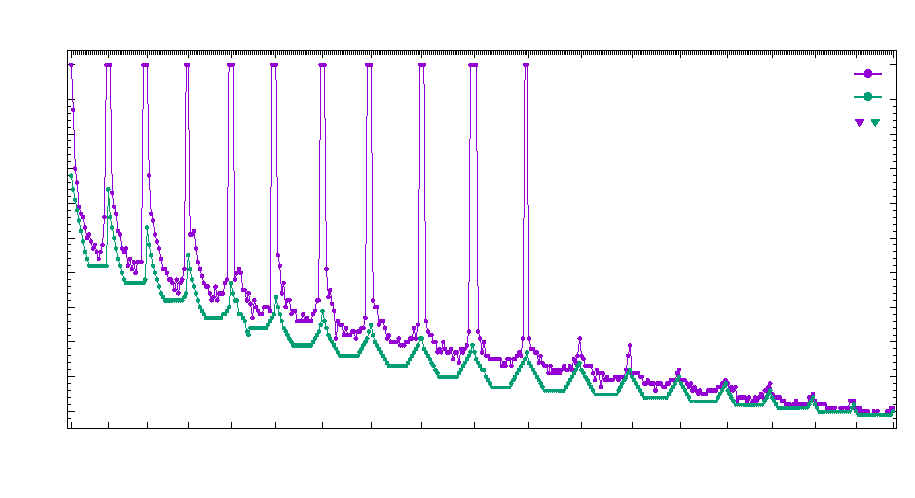
\includegraphics{resultados_6x6}}%
    \gplfronttext
  \end{picture}%
\endgroup
%
	\end{figure}
	}%
\end{frame}

\begin{frame}{Ejemplo ilustrativo en malla de $\mathsf{6\times 6}$}
	\vskip -7pt%
	\begin{figure}[H]
		\caption{Acomodo aleatorio inicial (izquierda) y acomodo encontrado por el algoritmo (derecha), mostrados en diferentes vistas.}%
		\arregloAntesDespues{caso=6x6, separacionAntesDespues=4, separacionVertical=0.3cm}{width=4.1cm}[width=4.2413cm]{width=2.9cm}%
	\end{figure}
\end{frame}
	

\begin{frame}{Mallas de $\mathsf{5\times 8}$}
	\vfill
	\Wider[1.85cm]{
	\begin{figure}[H]
		% GNUPLOT: LaTeX picture with Postscript
\begingroup
  % Encoding inside the plot.  In the header of your document, this encoding
  % should to defined, e.g., by using
  % \usepackage[latin1,<other encodings>]{inputenc}
  \inputencoding{latin1}%
  \makeatletter
  \providecommand\color[2][]{%
    \GenericError{(gnuplot) \space\space\space\@spaces}{%
      Package color not loaded in conjunction with
      terminal option `colourtext'%
    }{See the gnuplot documentation for explanation.%
    }{Either use 'blacktext' in gnuplot or load the package
      color.sty in LaTeX.}%
    \renewcommand\color[2][]{}%
  }%
  \providecommand\includegraphics[2][]{%
    \GenericError{(gnuplot) \space\space\space\@spaces}{%
      Package graphicx or graphics not loaded%
    }{See the gnuplot documentation for explanation.%
    }{The gnuplot epslatex terminal needs graphicx.sty or graphics.sty.}%
    \renewcommand\includegraphics[2][]{}%
  }%
  \providecommand\rotatebox[2]{#2}%
  \@ifundefined{ifGPcolor}{%
    \newif\ifGPcolor
    \GPcolortrue
  }{}%
  \@ifundefined{ifGPblacktext}{%
    \newif\ifGPblacktext
    \GPblacktexttrue
  }{}%
  % define a \g@addto@macro without @ in the name:
  \let\gplgaddtomacro\g@addto@macro
  % define empty templates for all commands taking text:
  \gdef\gplbacktext{}%
  \gdef\gplfronttext{}%
  \makeatother
  \ifGPblacktext
    % no textcolor at all
    \def\colorrgb#1{}%
    \def\colorgray#1{}%
  \else
    % gray or color?
    \ifGPcolor
      \def\colorrgb#1{\color[rgb]{#1}}%
      \def\colorgray#1{\color[gray]{#1}}%
      \expandafter\def\csname LTw\endcsname{\color{white}}%
      \expandafter\def\csname LTb\endcsname{\color{black}}%
      \expandafter\def\csname LTa\endcsname{\color{black}}%
      \expandafter\def\csname LT0\endcsname{\color[rgb]{1,0,0}}%
      \expandafter\def\csname LT1\endcsname{\color[rgb]{0,1,0}}%
      \expandafter\def\csname LT2\endcsname{\color[rgb]{0,0,1}}%
      \expandafter\def\csname LT3\endcsname{\color[rgb]{1,0,1}}%
      \expandafter\def\csname LT4\endcsname{\color[rgb]{0,1,1}}%
      \expandafter\def\csname LT5\endcsname{\color[rgb]{1,1,0}}%
      \expandafter\def\csname LT6\endcsname{\color[rgb]{0,0,0}}%
      \expandafter\def\csname LT7\endcsname{\color[rgb]{1,0.3,0}}%
      \expandafter\def\csname LT8\endcsname{\color[rgb]{0.5,0.5,0.5}}%
    \else
      % gray
      \def\colorrgb#1{\color{black}}%
      \def\colorgray#1{\color[gray]{#1}}%
      \expandafter\def\csname LTw\endcsname{\color{white}}%
      \expandafter\def\csname LTb\endcsname{\color{black}}%
      \expandafter\def\csname LTa\endcsname{\color{black}}%
      \expandafter\def\csname LT0\endcsname{\color{black}}%
      \expandafter\def\csname LT1\endcsname{\color{black}}%
      \expandafter\def\csname LT2\endcsname{\color{black}}%
      \expandafter\def\csname LT3\endcsname{\color{black}}%
      \expandafter\def\csname LT4\endcsname{\color{black}}%
      \expandafter\def\csname LT5\endcsname{\color{black}}%
      \expandafter\def\csname LT6\endcsname{\color{black}}%
      \expandafter\def\csname LT7\endcsname{\color{black}}%
      \expandafter\def\csname LT8\endcsname{\color{black}}%
    \fi
  \fi
    \setlength{\unitlength}{0.0500bp}%
    \ifx\gptboxheight\undefined%
      \newlength{\gptboxheight}%
      \newlength{\gptboxwidth}%
      \newsavebox{\gptboxtext}%
    \fi%
    \setlength{\fboxrule}{0.5pt}%
    \setlength{\fboxsep}{1pt}%
\begin{picture}(8466.00,4464.00)%
    \gplgaddtomacro\gplbacktext{%
      \csname LTb\endcsname%%
      \put(448,4000){\makebox(0,0)[r]{\strut{}\raisebox{2pt}{\fontsize{9}{9}\selectfont{$\infty$}}}}%
      \put(448,672){\makebox(0,0)[r]{\strut{}\fontsize{9}{9}\selectfont{20}}}%
      \put(448,1005){\makebox(0,0)[r]{\strut{}\fontsize{9}{9}\selectfont{30}}}%
      \put(448,1338){\makebox(0,0)[r]{\strut{}\fontsize{9}{9}\selectfont{40}}}%
      \put(448,1671){\makebox(0,0)[r]{\strut{}\fontsize{9}{9}\selectfont{50}}}%
      \put(448,2003){\makebox(0,0)[r]{\strut{}\fontsize{9}{9}\selectfont{60}}}%
      \put(448,2336){\makebox(0,0)[r]{\strut{}\fontsize{9}{9}\selectfont{70}}}%
      \put(448,2669){\makebox(0,0)[r]{\strut{}\fontsize{9}{9}\selectfont{80}}}%
      \put(448,3002){\makebox(0,0)[r]{\strut{}\fontsize{9}{9}\selectfont{90}}}%
      \put(448,3334){\makebox(0,0)[r]{\strut{}\fontsize{9}{9}\selectfont{100}}}%
      \put(448,3667){\makebox(0,0)[r]{\strut{}\fontsize{9}{9}\selectfont{110}}}%
      \put(384,308){\rotatebox{30}{\makebox(0,0)[l]{\strut{}\fontsize{7.7}{7.7}\selectfont{32,8}}}}%
      \put(739,308){\rotatebox{30}{\makebox(0,0)[l]{\strut{}\fontsize{7.7}{7.7}\selectfont{32,7}}}}%
      \put(1108,308){\rotatebox{30}{\makebox(0,0)[l]{\strut{}\fontsize{7.7}{7.7}\selectfont{32,6}}}}%
      \put(1492,308){\rotatebox{30}{\makebox(0,0)[l]{\strut{}\fontsize{7.7}{7.7}\selectfont{32,5}}}}%
      \put(1889,308){\rotatebox{30}{\makebox(0,0)[l]{\strut{}\fontsize{7.7}{7.7}\selectfont{32,4}}}}%
      \put(2301,308){\rotatebox{30}{\makebox(0,0)[l]{\strut{}\fontsize{7.7}{7.7}\selectfont{32,3}}}}%
      \put(2726,308){\rotatebox{30}{\makebox(0,0)[l]{\strut{}\fontsize{7.7}{7.7}\selectfont{32,2}}}}%
      \put(3166,308){\rotatebox{30}{\makebox(0,0)[l]{\strut{}\fontsize{7.7}{7.7}\selectfont{32,1}}}}%
      \put(3621,308){\rotatebox{30}{\makebox(0,0)[l]{\strut{}\fontsize{7.7}{7.7}\selectfont{32,0}}}}%
      \put(4089,308){\rotatebox{30}{\makebox(0,0)[l]{\strut{}\fontsize{7.7}{7.7}\selectfont{31,0}}}}%
      \put(4543,308){\rotatebox{30}{\makebox(0,0)[l]{\strut{}\fontsize{7.7}{7.7}\selectfont{30,0}}}}%
      \put(4983,308){\rotatebox{30}{\makebox(0,0)[l]{\strut{}\fontsize{7.7}{7.7}\selectfont{29,0}}}}%
      \put(5409,308){\rotatebox{30}{\makebox(0,0)[l]{\strut{}\fontsize{7.7}{7.7}\selectfont{28,0}}}}%
      \put(5821,308){\rotatebox{30}{\makebox(0,0)[l]{\strut{}\fontsize{7.7}{7.7}\selectfont{27,0}}}}%
      \put(6218,308){\rotatebox{30}{\makebox(0,0)[l]{\strut{}\fontsize{7.7}{7.7}\selectfont{26,0}}}}%
      \put(6601,308){\rotatebox{30}{\makebox(0,0)[l]{\strut{}\fontsize{7.7}{7.7}\selectfont{25,0}}}}%
      \put(6971,308){\rotatebox{30}{\makebox(0,0)[l]{\strut{}\fontsize{7.7}{7.7}\selectfont{24,0}}}}%
      \put(7325,308){\rotatebox{30}{\makebox(0,0)[l]{\strut{}\fontsize{7.7}{7.7}\selectfont{23,0}}}}%
      \put(7666,308){\rotatebox{30}{\makebox(0,0)[l]{\strut{}\fontsize{7.7}{7.7}\selectfont{22,0}}}}%
      \put(7993,308){\rotatebox{30}{\makebox(0,0)[l]{\strut{}\fontsize{7.7}{7.7}\selectfont{21,0}}}}%
      \put(8291,308){\rotatebox{30}{\makebox(0,0)[l]{\strut{}\fontsize{7.7}{7.7}\selectfont{0,21}}}}%
      \put(459,4144){\rotatebox{90}{\makebox(0,0)[l]{\strut{}\fontsize{0.4}{0.4}\selectfont{31,9}}}}%
      \put(473,4144){\rotatebox{90}{\makebox(0,0)[l]{\strut{}\fontsize{0.4}{0.4}\selectfont{30,10}}}}%
      \put(487,4144){\rotatebox{90}{\makebox(0,0)[l]{\strut{}\fontsize{0.4}{0.4}\selectfont{29,11}}}}%
      \put(501,4144){\rotatebox{90}{\makebox(0,0)[l]{\strut{}\fontsize{0.4}{0.4}\selectfont{28,12}}}}%
      \put(515,4144){\rotatebox{90}{\makebox(0,0)[l]{\strut{}\fontsize{0.4}{0.4}\selectfont{27,13}}}}%
      \put(530,4144){\rotatebox{90}{\makebox(0,0)[l]{\strut{}\fontsize{0.4}{0.4}\selectfont{26,14}}}}%
      \put(544,4144){\rotatebox{90}{\makebox(0,0)[l]{\strut{}\fontsize{0.4}{0.4}\selectfont{25,15}}}}%
      \put(558,4144){\rotatebox{90}{\makebox(0,0)[l]{\strut{}\fontsize{0.4}{0.4}\selectfont{24,16}}}}%
      \put(572,4144){\rotatebox{90}{\makebox(0,0)[l]{\strut{}\fontsize{0.4}{0.4}\selectfont{23,17}}}}%
      \put(586,4144){\rotatebox{90}{\makebox(0,0)[l]{\strut{}\fontsize{0.4}{0.4}\selectfont{22,18}}}}%
      \put(601,4144){\rotatebox{90}{\makebox(0,0)[l]{\strut{}\fontsize{0.4}{0.4}\selectfont{21,19}}}}%
      \put(615,4144){\rotatebox{90}{\makebox(0,0)[l]{\strut{}\fontsize{0.4}{0.4}\selectfont{20,20}}}}%
      \put(629,4144){\rotatebox{90}{\makebox(0,0)[l]{\strut{}\fontsize{0.4}{0.4}\selectfont{19,21}}}}%
      \put(643,4144){\rotatebox{90}{\makebox(0,0)[l]{\strut{}\fontsize{0.4}{0.4}\selectfont{18,22}}}}%
      \put(657,4144){\rotatebox{90}{\makebox(0,0)[l]{\strut{}\fontsize{0.4}{0.4}\selectfont{17,23}}}}%
      \put(671,4144){\rotatebox{90}{\makebox(0,0)[l]{\strut{}\fontsize{0.4}{0.4}\selectfont{16,24}}}}%
      \put(686,4144){\rotatebox{90}{\makebox(0,0)[l]{\strut{}\fontsize{0.4}{0.4}\selectfont{15,25}}}}%
      \put(700,4144){\rotatebox{90}{\makebox(0,0)[l]{\strut{}\fontsize{0.4}{0.4}\selectfont{14,26}}}}%
      \put(714,4144){\rotatebox{90}{\makebox(0,0)[l]{\strut{}\fontsize{0.4}{0.4}\selectfont{13,27}}}}%
      \put(728,4144){\rotatebox{90}{\makebox(0,0)[l]{\strut{}\fontsize{0.4}{0.4}\selectfont{12,28}}}}%
      \put(742,4144){\rotatebox{90}{\makebox(0,0)[l]{\strut{}\fontsize{0.4}{0.4}\selectfont{11,29}}}}%
      \put(757,4144){\rotatebox{90}{\makebox(0,0)[l]{\strut{}\fontsize{0.4}{0.4}\selectfont{10,30}}}}%
      \put(771,4144){\rotatebox{90}{\makebox(0,0)[l]{\strut{}\fontsize{0.4}{0.4}\selectfont{9,31}}}}%
      \put(785,4144){\rotatebox{90}{\makebox(0,0)[l]{\strut{}\fontsize{0.4}{0.4}\selectfont{8,32}}}}%
      \put(813,4144){\rotatebox{90}{\makebox(0,0)[l]{\strut{}\fontsize{0.4}{0.4}\selectfont{31,8}}}}%
      \put(828,4144){\rotatebox{90}{\makebox(0,0)[l]{\strut{}\fontsize{0.4}{0.4}\selectfont{30,9}}}}%
      \put(842,4144){\rotatebox{90}{\makebox(0,0)[l]{\strut{}\fontsize{0.4}{0.4}\selectfont{29,10}}}}%
      \put(856,4144){\rotatebox{90}{\makebox(0,0)[l]{\strut{}\fontsize{0.4}{0.4}\selectfont{28,11}}}}%
      \put(870,4144){\rotatebox{90}{\makebox(0,0)[l]{\strut{}\fontsize{0.4}{0.4}\selectfont{27,12}}}}%
      \put(884,4144){\rotatebox{90}{\makebox(0,0)[l]{\strut{}\fontsize{0.4}{0.4}\selectfont{26,13}}}}%
      \put(899,4144){\rotatebox{90}{\makebox(0,0)[l]{\strut{}\fontsize{0.4}{0.4}\selectfont{25,14}}}}%
      \put(913,4144){\rotatebox{90}{\makebox(0,0)[l]{\strut{}\fontsize{0.4}{0.4}\selectfont{24,15}}}}%
      \put(927,4144){\rotatebox{90}{\makebox(0,0)[l]{\strut{}\fontsize{0.4}{0.4}\selectfont{23,16}}}}%
      \put(941,4144){\rotatebox{90}{\makebox(0,0)[l]{\strut{}\fontsize{0.4}{0.4}\selectfont{22,17}}}}%
      \put(955,4144){\rotatebox{90}{\makebox(0,0)[l]{\strut{}\fontsize{0.4}{0.4}\selectfont{21,18}}}}%
      \put(970,4144){\rotatebox{90}{\makebox(0,0)[l]{\strut{}\fontsize{0.4}{0.4}\selectfont{20,19}}}}%
      \put(984,4144){\rotatebox{90}{\makebox(0,0)[l]{\strut{}\fontsize{0.4}{0.4}\selectfont{19,20}}}}%
      \put(998,4144){\rotatebox{90}{\makebox(0,0)[l]{\strut{}\fontsize{0.4}{0.4}\selectfont{18,21}}}}%
      \put(1012,4144){\rotatebox{90}{\makebox(0,0)[l]{\strut{}\fontsize{0.4}{0.4}\selectfont{17,22}}}}%
      \put(1026,4144){\rotatebox{90}{\makebox(0,0)[l]{\strut{}\fontsize{0.4}{0.4}\selectfont{16,23}}}}%
      \put(1041,4144){\rotatebox{90}{\makebox(0,0)[l]{\strut{}\fontsize{0.4}{0.4}\selectfont{15,24}}}}%
      \put(1055,4144){\rotatebox{90}{\makebox(0,0)[l]{\strut{}\fontsize{0.4}{0.4}\selectfont{14,25}}}}%
      \put(1069,4144){\rotatebox{90}{\makebox(0,0)[l]{\strut{}\fontsize{0.4}{0.4}\selectfont{13,26}}}}%
      \put(1083,4144){\rotatebox{90}{\makebox(0,0)[l]{\strut{}\fontsize{0.4}{0.4}\selectfont{12,27}}}}%
      \put(1097,4144){\rotatebox{90}{\makebox(0,0)[l]{\strut{}\fontsize{0.4}{0.4}\selectfont{11,28}}}}%
      \put(1112,4144){\rotatebox{90}{\makebox(0,0)[l]{\strut{}\fontsize{0.4}{0.4}\selectfont{10,29}}}}%
      \put(1126,4144){\rotatebox{90}{\makebox(0,0)[l]{\strut{}\fontsize{0.4}{0.4}\selectfont{9,30}}}}%
      \put(1140,4144){\rotatebox{90}{\makebox(0,0)[l]{\strut{}\fontsize{0.4}{0.4}\selectfont{8,31}}}}%
      \put(1154,4144){\rotatebox{90}{\makebox(0,0)[l]{\strut{}\fontsize{0.4}{0.4}\selectfont{7,32}}}}%
      \put(1182,4144){\rotatebox{90}{\makebox(0,0)[l]{\strut{}\fontsize{0.4}{0.4}\selectfont{31,7}}}}%
      \put(1197,4144){\rotatebox{90}{\makebox(0,0)[l]{\strut{}\fontsize{0.4}{0.4}\selectfont{30,8}}}}%
      \put(1211,4144){\rotatebox{90}{\makebox(0,0)[l]{\strut{}\fontsize{0.4}{0.4}\selectfont{29,9}}}}%
      \put(1225,4144){\rotatebox{90}{\makebox(0,0)[l]{\strut{}\fontsize{0.4}{0.4}\selectfont{28,10}}}}%
      \put(1239,4144){\rotatebox{90}{\makebox(0,0)[l]{\strut{}\fontsize{0.4}{0.4}\selectfont{27,11}}}}%
      \put(1253,4144){\rotatebox{90}{\makebox(0,0)[l]{\strut{}\fontsize{0.4}{0.4}\selectfont{26,12}}}}%
      \put(1268,4144){\rotatebox{90}{\makebox(0,0)[l]{\strut{}\fontsize{0.4}{0.4}\selectfont{25,13}}}}%
      \put(1282,4144){\rotatebox{90}{\makebox(0,0)[l]{\strut{}\fontsize{0.4}{0.4}\selectfont{24,14}}}}%
      \put(1296,4144){\rotatebox{90}{\makebox(0,0)[l]{\strut{}\fontsize{0.4}{0.4}\selectfont{23,15}}}}%
      \put(1310,4144){\rotatebox{90}{\makebox(0,0)[l]{\strut{}\fontsize{0.4}{0.4}\selectfont{22,16}}}}%
      \put(1324,4144){\rotatebox{90}{\makebox(0,0)[l]{\strut{}\fontsize{0.4}{0.4}\selectfont{21,17}}}}%
      \put(1339,4144){\rotatebox{90}{\makebox(0,0)[l]{\strut{}\fontsize{0.4}{0.4}\selectfont{20,18}}}}%
      \put(1353,4144){\rotatebox{90}{\makebox(0,0)[l]{\strut{}\fontsize{0.4}{0.4}\selectfont{19,19}}}}%
      \put(1367,4144){\rotatebox{90}{\makebox(0,0)[l]{\strut{}\fontsize{0.4}{0.4}\selectfont{18,20}}}}%
      \put(1381,4144){\rotatebox{90}{\makebox(0,0)[l]{\strut{}\fontsize{0.4}{0.4}\selectfont{17,21}}}}%
      \put(1395,4144){\rotatebox{90}{\makebox(0,0)[l]{\strut{}\fontsize{0.4}{0.4}\selectfont{16,22}}}}%
      \put(1410,4144){\rotatebox{90}{\makebox(0,0)[l]{\strut{}\fontsize{0.4}{0.4}\selectfont{15,23}}}}%
      \put(1424,4144){\rotatebox{90}{\makebox(0,0)[l]{\strut{}\fontsize{0.4}{0.4}\selectfont{14,24}}}}%
      \put(1438,4144){\rotatebox{90}{\makebox(0,0)[l]{\strut{}\fontsize{0.4}{0.4}\selectfont{13,25}}}}%
      \put(1452,4144){\rotatebox{90}{\makebox(0,0)[l]{\strut{}\fontsize{0.4}{0.4}\selectfont{12,26}}}}%
      \put(1466,4144){\rotatebox{90}{\makebox(0,0)[l]{\strut{}\fontsize{0.4}{0.4}\selectfont{11,27}}}}%
      \put(1481,4144){\rotatebox{90}{\makebox(0,0)[l]{\strut{}\fontsize{0.4}{0.4}\selectfont{10,28}}}}%
      \put(1495,4144){\rotatebox{90}{\makebox(0,0)[l]{\strut{}\fontsize{0.4}{0.4}\selectfont{9,29}}}}%
      \put(1509,4144){\rotatebox{90}{\makebox(0,0)[l]{\strut{}\fontsize{0.4}{0.4}\selectfont{8,30}}}}%
      \put(1523,4144){\rotatebox{90}{\makebox(0,0)[l]{\strut{}\fontsize{0.4}{0.4}\selectfont{7,31}}}}%
      \put(1537,4144){\rotatebox{90}{\makebox(0,0)[l]{\strut{}\fontsize{0.4}{0.4}\selectfont{6,32}}}}%
      \put(1566,4144){\rotatebox{90}{\makebox(0,0)[l]{\strut{}\fontsize{0.4}{0.4}\selectfont{31,6}}}}%
      \put(1580,4144){\rotatebox{90}{\makebox(0,0)[l]{\strut{}\fontsize{0.4}{0.4}\selectfont{30,7}}}}%
      \put(1594,4144){\rotatebox{90}{\makebox(0,0)[l]{\strut{}\fontsize{0.4}{0.4}\selectfont{29,8}}}}%
      \put(1608,4144){\rotatebox{90}{\makebox(0,0)[l]{\strut{}\fontsize{0.4}{0.4}\selectfont{28,9}}}}%
      \put(1623,4144){\rotatebox{90}{\makebox(0,0)[l]{\strut{}\fontsize{0.4}{0.4}\selectfont{27,10}}}}%
      \put(1637,4144){\rotatebox{90}{\makebox(0,0)[l]{\strut{}\fontsize{0.4}{0.4}\selectfont{26,11}}}}%
      \put(1651,4144){\rotatebox{90}{\makebox(0,0)[l]{\strut{}\fontsize{0.4}{0.4}\selectfont{25,12}}}}%
      \put(1665,4144){\rotatebox{90}{\makebox(0,0)[l]{\strut{}\fontsize{0.4}{0.4}\selectfont{24,13}}}}%
      \put(1679,4144){\rotatebox{90}{\makebox(0,0)[l]{\strut{}\fontsize{0.4}{0.4}\selectfont{23,14}}}}%
      \put(1693,4144){\rotatebox{90}{\makebox(0,0)[l]{\strut{}\fontsize{0.4}{0.4}\selectfont{22,15}}}}%
      \put(1708,4144){\rotatebox{90}{\makebox(0,0)[l]{\strut{}\fontsize{0.4}{0.4}\selectfont{21,16}}}}%
      \put(1722,4144){\rotatebox{90}{\makebox(0,0)[l]{\strut{}\fontsize{0.4}{0.4}\selectfont{20,17}}}}%
      \put(1736,4144){\rotatebox{90}{\makebox(0,0)[l]{\strut{}\fontsize{0.4}{0.4}\selectfont{19,18}}}}%
      \put(1750,4144){\rotatebox{90}{\makebox(0,0)[l]{\strut{}\fontsize{0.4}{0.4}\selectfont{18,19}}}}%
      \put(1764,4144){\rotatebox{90}{\makebox(0,0)[l]{\strut{}\fontsize{0.4}{0.4}\selectfont{17,20}}}}%
      \put(1779,4144){\rotatebox{90}{\makebox(0,0)[l]{\strut{}\fontsize{0.4}{0.4}\selectfont{16,21}}}}%
      \put(1793,4144){\rotatebox{90}{\makebox(0,0)[l]{\strut{}\fontsize{0.4}{0.4}\selectfont{15,22}}}}%
      \put(1807,4144){\rotatebox{90}{\makebox(0,0)[l]{\strut{}\fontsize{0.4}{0.4}\selectfont{14,23}}}}%
      \put(1821,4144){\rotatebox{90}{\makebox(0,0)[l]{\strut{}\fontsize{0.4}{0.4}\selectfont{13,24}}}}%
      \put(1835,4144){\rotatebox{90}{\makebox(0,0)[l]{\strut{}\fontsize{0.4}{0.4}\selectfont{12,25}}}}%
      \put(1850,4144){\rotatebox{90}{\makebox(0,0)[l]{\strut{}\fontsize{0.4}{0.4}\selectfont{11,26}}}}%
      \put(1864,4144){\rotatebox{90}{\makebox(0,0)[l]{\strut{}\fontsize{0.4}{0.4}\selectfont{10,27}}}}%
      \put(1878,4144){\rotatebox{90}{\makebox(0,0)[l]{\strut{}\fontsize{0.4}{0.4}\selectfont{9,28}}}}%
      \put(1892,4144){\rotatebox{90}{\makebox(0,0)[l]{\strut{}\fontsize{0.4}{0.4}\selectfont{8,29}}}}%
      \put(1906,4144){\rotatebox{90}{\makebox(0,0)[l]{\strut{}\fontsize{0.4}{0.4}\selectfont{7,30}}}}%
      \put(1921,4144){\rotatebox{90}{\makebox(0,0)[l]{\strut{}\fontsize{0.4}{0.4}\selectfont{6,31}}}}%
      \put(1935,4144){\rotatebox{90}{\makebox(0,0)[l]{\strut{}\fontsize{0.4}{0.4}\selectfont{5,32}}}}%
      \put(1963,4144){\rotatebox{90}{\makebox(0,0)[l]{\strut{}\fontsize{0.4}{0.4}\selectfont{31,5}}}}%
      \put(1977,4144){\rotatebox{90}{\makebox(0,0)[l]{\strut{}\fontsize{0.4}{0.4}\selectfont{30,6}}}}%
      \put(1992,4144){\rotatebox{90}{\makebox(0,0)[l]{\strut{}\fontsize{0.4}{0.4}\selectfont{29,7}}}}%
      \put(2006,4144){\rotatebox{90}{\makebox(0,0)[l]{\strut{}\fontsize{0.4}{0.4}\selectfont{28,8}}}}%
      \put(2020,4144){\rotatebox{90}{\makebox(0,0)[l]{\strut{}\fontsize{0.4}{0.4}\selectfont{27,9}}}}%
      \put(2034,4144){\rotatebox{90}{\makebox(0,0)[l]{\strut{}\fontsize{0.4}{0.4}\selectfont{26,10}}}}%
      \put(2048,4144){\rotatebox{90}{\makebox(0,0)[l]{\strut{}\fontsize{0.4}{0.4}\selectfont{25,11}}}}%
      \put(2063,4144){\rotatebox{90}{\makebox(0,0)[l]{\strut{}\fontsize{0.4}{0.4}\selectfont{24,12}}}}%
      \put(2077,4144){\rotatebox{90}{\makebox(0,0)[l]{\strut{}\fontsize{0.4}{0.4}\selectfont{23,13}}}}%
      \put(2091,4144){\rotatebox{90}{\makebox(0,0)[l]{\strut{}\fontsize{0.4}{0.4}\selectfont{22,14}}}}%
      \put(2105,4144){\rotatebox{90}{\makebox(0,0)[l]{\strut{}\fontsize{0.4}{0.4}\selectfont{21,15}}}}%
      \put(2119,4144){\rotatebox{90}{\makebox(0,0)[l]{\strut{}\fontsize{0.4}{0.4}\selectfont{20,16}}}}%
      \put(2134,4144){\rotatebox{90}{\makebox(0,0)[l]{\strut{}\fontsize{0.4}{0.4}\selectfont{19,17}}}}%
      \put(2148,4144){\rotatebox{90}{\makebox(0,0)[l]{\strut{}\fontsize{0.4}{0.4}\selectfont{18,18}}}}%
      \put(2162,4144){\rotatebox{90}{\makebox(0,0)[l]{\strut{}\fontsize{0.4}{0.4}\selectfont{17,19}}}}%
      \put(2176,4144){\rotatebox{90}{\makebox(0,0)[l]{\strut{}\fontsize{0.4}{0.4}\selectfont{16,20}}}}%
      \put(2190,4144){\rotatebox{90}{\makebox(0,0)[l]{\strut{}\fontsize{0.4}{0.4}\selectfont{15,21}}}}%
      \put(2204,4144){\rotatebox{90}{\makebox(0,0)[l]{\strut{}\fontsize{0.4}{0.4}\selectfont{14,22}}}}%
      \put(2219,4144){\rotatebox{90}{\makebox(0,0)[l]{\strut{}\fontsize{0.4}{0.4}\selectfont{13,23}}}}%
      \put(2233,4144){\rotatebox{90}{\makebox(0,0)[l]{\strut{}\fontsize{0.4}{0.4}\selectfont{12,24}}}}%
      \put(2247,4144){\rotatebox{90}{\makebox(0,0)[l]{\strut{}\fontsize{0.4}{0.4}\selectfont{11,25}}}}%
      \put(2261,4144){\rotatebox{90}{\makebox(0,0)[l]{\strut{}\fontsize{0.4}{0.4}\selectfont{10,26}}}}%
      \put(2275,4144){\rotatebox{90}{\makebox(0,0)[l]{\strut{}\fontsize{0.4}{0.4}\selectfont{9,27}}}}%
      \put(2290,4144){\rotatebox{90}{\makebox(0,0)[l]{\strut{}\fontsize{0.4}{0.4}\selectfont{8,28}}}}%
      \put(2304,4144){\rotatebox{90}{\makebox(0,0)[l]{\strut{}\fontsize{0.4}{0.4}\selectfont{7,29}}}}%
      \put(2318,4144){\rotatebox{90}{\makebox(0,0)[l]{\strut{}\fontsize{0.4}{0.4}\selectfont{6,30}}}}%
      \put(2332,4144){\rotatebox{90}{\makebox(0,0)[l]{\strut{}\fontsize{0.4}{0.4}\selectfont{5,31}}}}%
      \put(2346,4144){\rotatebox{90}{\makebox(0,0)[l]{\strut{}\fontsize{0.4}{0.4}\selectfont{4,32}}}}%
      \put(2375,4144){\rotatebox{90}{\makebox(0,0)[l]{\strut{}\fontsize{0.4}{0.4}\selectfont{31,4}}}}%
      \put(2389,4144){\rotatebox{90}{\makebox(0,0)[l]{\strut{}\fontsize{0.4}{0.4}\selectfont{30,5}}}}%
      \put(2403,4144){\rotatebox{90}{\makebox(0,0)[l]{\strut{}\fontsize{0.4}{0.4}\selectfont{29,6}}}}%
      \put(2417,4144){\rotatebox{90}{\makebox(0,0)[l]{\strut{}\fontsize{0.4}{0.4}\selectfont{28,7}}}}%
      \put(2432,4144){\rotatebox{90}{\makebox(0,0)[l]{\strut{}\fontsize{0.4}{0.4}\selectfont{27,8}}}}%
      \put(2446,4144){\rotatebox{90}{\makebox(0,0)[l]{\strut{}\fontsize{0.4}{0.4}\selectfont{26,9}}}}%
      \put(2460,4144){\rotatebox{90}{\makebox(0,0)[l]{\strut{}\fontsize{0.4}{0.4}\selectfont{25,10}}}}%
      \put(2474,4144){\rotatebox{90}{\makebox(0,0)[l]{\strut{}\fontsize{0.4}{0.4}\selectfont{24,11}}}}%
      \put(2488,4144){\rotatebox{90}{\makebox(0,0)[l]{\strut{}\fontsize{0.4}{0.4}\selectfont{23,12}}}}%
      \put(2503,4144){\rotatebox{90}{\makebox(0,0)[l]{\strut{}\fontsize{0.4}{0.4}\selectfont{22,13}}}}%
      \put(2517,4144){\rotatebox{90}{\makebox(0,0)[l]{\strut{}\fontsize{0.4}{0.4}\selectfont{21,14}}}}%
      \put(2531,4144){\rotatebox{90}{\makebox(0,0)[l]{\strut{}\fontsize{0.4}{0.4}\selectfont{20,15}}}}%
      \put(2545,4144){\rotatebox{90}{\makebox(0,0)[l]{\strut{}\fontsize{0.4}{0.4}\selectfont{19,16}}}}%
      \put(2559,4144){\rotatebox{90}{\makebox(0,0)[l]{\strut{}\fontsize{0.4}{0.4}\selectfont{18,17}}}}%
      \put(2574,4144){\rotatebox{90}{\makebox(0,0)[l]{\strut{}\fontsize{0.4}{0.4}\selectfont{17,18}}}}%
      \put(2588,4144){\rotatebox{90}{\makebox(0,0)[l]{\strut{}\fontsize{0.4}{0.4}\selectfont{16,19}}}}%
      \put(2602,4144){\rotatebox{90}{\makebox(0,0)[l]{\strut{}\fontsize{0.4}{0.4}\selectfont{15,20}}}}%
      \put(2616,4144){\rotatebox{90}{\makebox(0,0)[l]{\strut{}\fontsize{0.4}{0.4}\selectfont{14,21}}}}%
      \put(2630,4144){\rotatebox{90}{\makebox(0,0)[l]{\strut{}\fontsize{0.4}{0.4}\selectfont{13,22}}}}%
      \put(2645,4144){\rotatebox{90}{\makebox(0,0)[l]{\strut{}\fontsize{0.4}{0.4}\selectfont{12,23}}}}%
      \put(2659,4144){\rotatebox{90}{\makebox(0,0)[l]{\strut{}\fontsize{0.4}{0.4}\selectfont{11,24}}}}%
      \put(2673,4144){\rotatebox{90}{\makebox(0,0)[l]{\strut{}\fontsize{0.4}{0.4}\selectfont{10,25}}}}%
      \put(2687,4144){\rotatebox{90}{\makebox(0,0)[l]{\strut{}\fontsize{0.4}{0.4}\selectfont{9,26}}}}%
      \put(2701,4144){\rotatebox{90}{\makebox(0,0)[l]{\strut{}\fontsize{0.4}{0.4}\selectfont{8,27}}}}%
      \put(2715,4144){\rotatebox{90}{\makebox(0,0)[l]{\strut{}\fontsize{0.4}{0.4}\selectfont{7,28}}}}%
      \put(2730,4144){\rotatebox{90}{\makebox(0,0)[l]{\strut{}\fontsize{0.4}{0.4}\selectfont{6,29}}}}%
      \put(2744,4144){\rotatebox{90}{\makebox(0,0)[l]{\strut{}\fontsize{0.4}{0.4}\selectfont{5,30}}}}%
      \put(2758,4144){\rotatebox{90}{\makebox(0,0)[l]{\strut{}\fontsize{0.4}{0.4}\selectfont{4,31}}}}%
      \put(2772,4144){\rotatebox{90}{\makebox(0,0)[l]{\strut{}\fontsize{0.4}{0.4}\selectfont{3,32}}}}%
      \put(2801,4144){\rotatebox{90}{\makebox(0,0)[l]{\strut{}\fontsize{0.4}{0.4}\selectfont{31,3}}}}%
      \put(2815,4144){\rotatebox{90}{\makebox(0,0)[l]{\strut{}\fontsize{0.4}{0.4}\selectfont{30,4}}}}%
      \put(2829,4144){\rotatebox{90}{\makebox(0,0)[l]{\strut{}\fontsize{0.4}{0.4}\selectfont{29,5}}}}%
      \put(2843,4144){\rotatebox{90}{\makebox(0,0)[l]{\strut{}\fontsize{0.4}{0.4}\selectfont{28,6}}}}%
      \put(2857,4144){\rotatebox{90}{\makebox(0,0)[l]{\strut{}\fontsize{0.4}{0.4}\selectfont{27,7}}}}%
      \put(2872,4144){\rotatebox{90}{\makebox(0,0)[l]{\strut{}\fontsize{0.4}{0.4}\selectfont{26,8}}}}%
      \put(2886,4144){\rotatebox{90}{\makebox(0,0)[l]{\strut{}\fontsize{0.4}{0.4}\selectfont{25,9}}}}%
      \put(2900,4144){\rotatebox{90}{\makebox(0,0)[l]{\strut{}\fontsize{0.4}{0.4}\selectfont{24,10}}}}%
      \put(2914,4144){\rotatebox{90}{\makebox(0,0)[l]{\strut{}\fontsize{0.4}{0.4}\selectfont{23,11}}}}%
      \put(2928,4144){\rotatebox{90}{\makebox(0,0)[l]{\strut{}\fontsize{0.4}{0.4}\selectfont{22,12}}}}%
      \put(2943,4144){\rotatebox{90}{\makebox(0,0)[l]{\strut{}\fontsize{0.4}{0.4}\selectfont{21,13}}}}%
      \put(2957,4144){\rotatebox{90}{\makebox(0,0)[l]{\strut{}\fontsize{0.4}{0.4}\selectfont{20,14}}}}%
      \put(2971,4144){\rotatebox{90}{\makebox(0,0)[l]{\strut{}\fontsize{0.4}{0.4}\selectfont{19,15}}}}%
      \put(2985,4144){\rotatebox{90}{\makebox(0,0)[l]{\strut{}\fontsize{0.4}{0.4}\selectfont{18,16}}}}%
      \put(2999,4144){\rotatebox{90}{\makebox(0,0)[l]{\strut{}\fontsize{0.4}{0.4}\selectfont{17,17}}}}%
      \put(3014,4144){\rotatebox{90}{\makebox(0,0)[l]{\strut{}\fontsize{0.4}{0.4}\selectfont{16,18}}}}%
      \put(3028,4144){\rotatebox{90}{\makebox(0,0)[l]{\strut{}\fontsize{0.4}{0.4}\selectfont{15,19}}}}%
      \put(3042,4144){\rotatebox{90}{\makebox(0,0)[l]{\strut{}\fontsize{0.4}{0.4}\selectfont{14,20}}}}%
      \put(3056,4144){\rotatebox{90}{\makebox(0,0)[l]{\strut{}\fontsize{0.4}{0.4}\selectfont{13,21}}}}%
      \put(3070,4144){\rotatebox{90}{\makebox(0,0)[l]{\strut{}\fontsize{0.4}{0.4}\selectfont{12,22}}}}%
      \put(3085,4144){\rotatebox{90}{\makebox(0,0)[l]{\strut{}\fontsize{0.4}{0.4}\selectfont{11,23}}}}%
      \put(3099,4144){\rotatebox{90}{\makebox(0,0)[l]{\strut{}\fontsize{0.4}{0.4}\selectfont{10,24}}}}%
      \put(3113,4144){\rotatebox{90}{\makebox(0,0)[l]{\strut{}\fontsize{0.4}{0.4}\selectfont{9,25}}}}%
      \put(3127,4144){\rotatebox{90}{\makebox(0,0)[l]{\strut{}\fontsize{0.4}{0.4}\selectfont{8,26}}}}%
      \put(3141,4144){\rotatebox{90}{\makebox(0,0)[l]{\strut{}\fontsize{0.4}{0.4}\selectfont{7,27}}}}%
      \put(3155,4144){\rotatebox{90}{\makebox(0,0)[l]{\strut{}\fontsize{0.4}{0.4}\selectfont{6,28}}}}%
      \put(3170,4144){\rotatebox{90}{\makebox(0,0)[l]{\strut{}\fontsize{0.4}{0.4}\selectfont{5,29}}}}%
      \put(3184,4144){\rotatebox{90}{\makebox(0,0)[l]{\strut{}\fontsize{0.4}{0.4}\selectfont{4,30}}}}%
      \put(3198,4144){\rotatebox{90}{\makebox(0,0)[l]{\strut{}\fontsize{0.4}{0.4}\selectfont{3,31}}}}%
      \put(3212,4144){\rotatebox{90}{\makebox(0,0)[l]{\strut{}\fontsize{0.4}{0.4}\selectfont{2,32}}}}%
      \put(3241,4144){\rotatebox{90}{\makebox(0,0)[l]{\strut{}\fontsize{0.4}{0.4}\selectfont{31,2}}}}%
      \put(3255,4144){\rotatebox{90}{\makebox(0,0)[l]{\strut{}\fontsize{0.4}{0.4}\selectfont{30,3}}}}%
      \put(3269,4144){\rotatebox{90}{\makebox(0,0)[l]{\strut{}\fontsize{0.4}{0.4}\selectfont{29,4}}}}%
      \put(3283,4144){\rotatebox{90}{\makebox(0,0)[l]{\strut{}\fontsize{0.4}{0.4}\selectfont{28,5}}}}%
      \put(3297,4144){\rotatebox{90}{\makebox(0,0)[l]{\strut{}\fontsize{0.4}{0.4}\selectfont{27,6}}}}%
      \put(3312,4144){\rotatebox{90}{\makebox(0,0)[l]{\strut{}\fontsize{0.4}{0.4}\selectfont{26,7}}}}%
      \put(3326,4144){\rotatebox{90}{\makebox(0,0)[l]{\strut{}\fontsize{0.4}{0.4}\selectfont{25,8}}}}%
      \put(3340,4144){\rotatebox{90}{\makebox(0,0)[l]{\strut{}\fontsize{0.4}{0.4}\selectfont{24,9}}}}%
      \put(3354,4144){\rotatebox{90}{\makebox(0,0)[l]{\strut{}\fontsize{0.4}{0.4}\selectfont{23,10}}}}%
      \put(3368,4144){\rotatebox{90}{\makebox(0,0)[l]{\strut{}\fontsize{0.4}{0.4}\selectfont{22,11}}}}%
      \put(3383,4144){\rotatebox{90}{\makebox(0,0)[l]{\strut{}\fontsize{0.4}{0.4}\selectfont{21,12}}}}%
      \put(3397,4144){\rotatebox{90}{\makebox(0,0)[l]{\strut{}\fontsize{0.4}{0.4}\selectfont{20,13}}}}%
      \put(3411,4144){\rotatebox{90}{\makebox(0,0)[l]{\strut{}\fontsize{0.4}{0.4}\selectfont{19,14}}}}%
      \put(3425,4144){\rotatebox{90}{\makebox(0,0)[l]{\strut{}\fontsize{0.4}{0.4}\selectfont{18,15}}}}%
      \put(3439,4144){\rotatebox{90}{\makebox(0,0)[l]{\strut{}\fontsize{0.4}{0.4}\selectfont{17,16}}}}%
      \put(3454,4144){\rotatebox{90}{\makebox(0,0)[l]{\strut{}\fontsize{0.4}{0.4}\selectfont{16,17}}}}%
      \put(3468,4144){\rotatebox{90}{\makebox(0,0)[l]{\strut{}\fontsize{0.4}{0.4}\selectfont{15,18}}}}%
      \put(3482,4144){\rotatebox{90}{\makebox(0,0)[l]{\strut{}\fontsize{0.4}{0.4}\selectfont{14,19}}}}%
      \put(3496,4144){\rotatebox{90}{\makebox(0,0)[l]{\strut{}\fontsize{0.4}{0.4}\selectfont{13,20}}}}%
      \put(3510,4144){\rotatebox{90}{\makebox(0,0)[l]{\strut{}\fontsize{0.4}{0.4}\selectfont{12,21}}}}%
      \put(3525,4144){\rotatebox{90}{\makebox(0,0)[l]{\strut{}\fontsize{0.4}{0.4}\selectfont{11,22}}}}%
      \put(3539,4144){\rotatebox{90}{\makebox(0,0)[l]{\strut{}\fontsize{0.4}{0.4}\selectfont{10,23}}}}%
      \put(3553,4144){\rotatebox{90}{\makebox(0,0)[l]{\strut{}\fontsize{0.4}{0.4}\selectfont{9,24}}}}%
      \put(3567,4144){\rotatebox{90}{\makebox(0,0)[l]{\strut{}\fontsize{0.4}{0.4}\selectfont{8,25}}}}%
      \put(3581,4144){\rotatebox{90}{\makebox(0,0)[l]{\strut{}\fontsize{0.4}{0.4}\selectfont{7,26}}}}%
      \put(3596,4144){\rotatebox{90}{\makebox(0,0)[l]{\strut{}\fontsize{0.4}{0.4}\selectfont{6,27}}}}%
      \put(3610,4144){\rotatebox{90}{\makebox(0,0)[l]{\strut{}\fontsize{0.4}{0.4}\selectfont{5,28}}}}%
      \put(3624,4144){\rotatebox{90}{\makebox(0,0)[l]{\strut{}\fontsize{0.4}{0.4}\selectfont{4,29}}}}%
      \put(3638,4144){\rotatebox{90}{\makebox(0,0)[l]{\strut{}\fontsize{0.4}{0.4}\selectfont{3,30}}}}%
      \put(3652,4144){\rotatebox{90}{\makebox(0,0)[l]{\strut{}\fontsize{0.4}{0.4}\selectfont{2,31}}}}%
      \put(3666,4144){\rotatebox{90}{\makebox(0,0)[l]{\strut{}\fontsize{0.4}{0.4}\selectfont{1,32}}}}%
      \put(3695,4144){\rotatebox{90}{\makebox(0,0)[l]{\strut{}\fontsize{0.4}{0.4}\selectfont{31,1}}}}%
      \put(3709,4144){\rotatebox{90}{\makebox(0,0)[l]{\strut{}\fontsize{0.4}{0.4}\selectfont{30,2}}}}%
      \put(3723,4144){\rotatebox{90}{\makebox(0,0)[l]{\strut{}\fontsize{0.4}{0.4}\selectfont{29,3}}}}%
      \put(3737,4144){\rotatebox{90}{\makebox(0,0)[l]{\strut{}\fontsize{0.4}{0.4}\selectfont{28,4}}}}%
      \put(3752,4144){\rotatebox{90}{\makebox(0,0)[l]{\strut{}\fontsize{0.4}{0.4}\selectfont{27,5}}}}%
      \put(3766,4144){\rotatebox{90}{\makebox(0,0)[l]{\strut{}\fontsize{0.4}{0.4}\selectfont{26,6}}}}%
      \put(3780,4144){\rotatebox{90}{\makebox(0,0)[l]{\strut{}\fontsize{0.4}{0.4}\selectfont{25,7}}}}%
      \put(3794,4144){\rotatebox{90}{\makebox(0,0)[l]{\strut{}\fontsize{0.4}{0.4}\selectfont{24,8}}}}%
      \put(3808,4144){\rotatebox{90}{\makebox(0,0)[l]{\strut{}\fontsize{0.4}{0.4}\selectfont{23,9}}}}%
      \put(3823,4144){\rotatebox{90}{\makebox(0,0)[l]{\strut{}\fontsize{0.4}{0.4}\selectfont{22,10}}}}%
      \put(3837,4144){\rotatebox{90}{\makebox(0,0)[l]{\strut{}\fontsize{0.4}{0.4}\selectfont{21,11}}}}%
      \put(3851,4144){\rotatebox{90}{\makebox(0,0)[l]{\strut{}\fontsize{0.4}{0.4}\selectfont{20,12}}}}%
      \put(3865,4144){\rotatebox{90}{\makebox(0,0)[l]{\strut{}\fontsize{0.4}{0.4}\selectfont{19,13}}}}%
      \put(3879,4144){\rotatebox{90}{\makebox(0,0)[l]{\strut{}\fontsize{0.4}{0.4}\selectfont{18,14}}}}%
      \put(3894,4144){\rotatebox{90}{\makebox(0,0)[l]{\strut{}\fontsize{0.4}{0.4}\selectfont{17,15}}}}%
      \put(3908,4144){\rotatebox{90}{\makebox(0,0)[l]{\strut{}\fontsize{0.4}{0.4}\selectfont{16,16}}}}%
      \put(3922,4144){\rotatebox{90}{\makebox(0,0)[l]{\strut{}\fontsize{0.4}{0.4}\selectfont{15,17}}}}%
      \put(3936,4144){\rotatebox{90}{\makebox(0,0)[l]{\strut{}\fontsize{0.4}{0.4}\selectfont{14,18}}}}%
      \put(3950,4144){\rotatebox{90}{\makebox(0,0)[l]{\strut{}\fontsize{0.4}{0.4}\selectfont{13,19}}}}%
      \put(3965,4144){\rotatebox{90}{\makebox(0,0)[l]{\strut{}\fontsize{0.4}{0.4}\selectfont{12,20}}}}%
      \put(3979,4144){\rotatebox{90}{\makebox(0,0)[l]{\strut{}\fontsize{0.4}{0.4}\selectfont{11,21}}}}%
      \put(3993,4144){\rotatebox{90}{\makebox(0,0)[l]{\strut{}\fontsize{0.4}{0.4}\selectfont{10,22}}}}%
      \put(4007,4144){\rotatebox{90}{\makebox(0,0)[l]{\strut{}\fontsize{0.4}{0.4}\selectfont{9,23}}}}%
      \put(4021,4144){\rotatebox{90}{\makebox(0,0)[l]{\strut{}\fontsize{0.4}{0.4}\selectfont{8,24}}}}%
      \put(4036,4144){\rotatebox{90}{\makebox(0,0)[l]{\strut{}\fontsize{0.4}{0.4}\selectfont{7,25}}}}%
      \put(4050,4144){\rotatebox{90}{\makebox(0,0)[l]{\strut{}\fontsize{0.4}{0.4}\selectfont{6,26}}}}%
      \put(4064,4144){\rotatebox{90}{\makebox(0,0)[l]{\strut{}\fontsize{0.4}{0.4}\selectfont{5,27}}}}%
      \put(4078,4144){\rotatebox{90}{\makebox(0,0)[l]{\strut{}\fontsize{0.4}{0.4}\selectfont{4,28}}}}%
      \put(4092,4144){\rotatebox{90}{\makebox(0,0)[l]{\strut{}\fontsize{0.4}{0.4}\selectfont{3,29}}}}%
      \put(4107,4144){\rotatebox{90}{\makebox(0,0)[l]{\strut{}\fontsize{0.4}{0.4}\selectfont{2,30}}}}%
      \put(4121,4144){\rotatebox{90}{\makebox(0,0)[l]{\strut{}\fontsize{0.4}{0.4}\selectfont{1,31}}}}%
      \put(4135,4144){\rotatebox{90}{\makebox(0,0)[l]{\strut{}\fontsize{0.4}{0.4}\selectfont{0,32}}}}%
      \put(4163,4144){\rotatebox{90}{\makebox(0,0)[l]{\strut{}\fontsize{0.4}{0.4}\selectfont{30,1}}}}%
      \put(4177,4144){\rotatebox{90}{\makebox(0,0)[l]{\strut{}\fontsize{0.4}{0.4}\selectfont{29,2}}}}%
      \put(4192,4144){\rotatebox{90}{\makebox(0,0)[l]{\strut{}\fontsize{0.4}{0.4}\selectfont{28,3}}}}%
      \put(4206,4144){\rotatebox{90}{\makebox(0,0)[l]{\strut{}\fontsize{0.4}{0.4}\selectfont{27,4}}}}%
      \put(4220,4144){\rotatebox{90}{\makebox(0,0)[l]{\strut{}\fontsize{0.4}{0.4}\selectfont{26,5}}}}%
      \put(4234,4144){\rotatebox{90}{\makebox(0,0)[l]{\strut{}\fontsize{0.4}{0.4}\selectfont{25,6}}}}%
      \put(4248,4144){\rotatebox{90}{\makebox(0,0)[l]{\strut{}\fontsize{0.4}{0.4}\selectfont{24,7}}}}%
      \put(4263,4144){\rotatebox{90}{\makebox(0,0)[l]{\strut{}\fontsize{0.4}{0.4}\selectfont{23,8}}}}%
      \put(4277,4144){\rotatebox{90}{\makebox(0,0)[l]{\strut{}\fontsize{0.4}{0.4}\selectfont{22,9}}}}%
      \put(4291,4144){\rotatebox{90}{\makebox(0,0)[l]{\strut{}\fontsize{0.4}{0.4}\selectfont{21,10}}}}%
      \put(4305,4144){\rotatebox{90}{\makebox(0,0)[l]{\strut{}\fontsize{0.4}{0.4}\selectfont{20,11}}}}%
      \put(4319,4144){\rotatebox{90}{\makebox(0,0)[l]{\strut{}\fontsize{0.4}{0.4}\selectfont{19,12}}}}%
      \put(4334,4144){\rotatebox{90}{\makebox(0,0)[l]{\strut{}\fontsize{0.4}{0.4}\selectfont{18,13}}}}%
      \put(4348,4144){\rotatebox{90}{\makebox(0,0)[l]{\strut{}\fontsize{0.4}{0.4}\selectfont{17,14}}}}%
      \put(4362,4144){\rotatebox{90}{\makebox(0,0)[l]{\strut{}\fontsize{0.4}{0.4}\selectfont{16,15}}}}%
      \put(4376,4144){\rotatebox{90}{\makebox(0,0)[l]{\strut{}\fontsize{0.4}{0.4}\selectfont{15,16}}}}%
      \put(4390,4144){\rotatebox{90}{\makebox(0,0)[l]{\strut{}\fontsize{0.4}{0.4}\selectfont{14,17}}}}%
      \put(4405,4144){\rotatebox{90}{\makebox(0,0)[l]{\strut{}\fontsize{0.4}{0.4}\selectfont{13,18}}}}%
      \put(4419,4144){\rotatebox{90}{\makebox(0,0)[l]{\strut{}\fontsize{0.4}{0.4}\selectfont{12,19}}}}%
      \put(4433,4144){\rotatebox{90}{\makebox(0,0)[l]{\strut{}\fontsize{0.4}{0.4}\selectfont{11,20}}}}%
      \put(4447,4144){\rotatebox{90}{\makebox(0,0)[l]{\strut{}\fontsize{0.4}{0.4}\selectfont{10,21}}}}%
      \put(4461,4144){\rotatebox{90}{\makebox(0,0)[l]{\strut{}\fontsize{0.4}{0.4}\selectfont{9,22}}}}%
      \put(4476,4144){\rotatebox{90}{\makebox(0,0)[l]{\strut{}\fontsize{0.4}{0.4}\selectfont{8,23}}}}%
      \put(4490,4144){\rotatebox{90}{\makebox(0,0)[l]{\strut{}\fontsize{0.4}{0.4}\selectfont{7,24}}}}%
      \put(4504,4144){\rotatebox{90}{\makebox(0,0)[l]{\strut{}\fontsize{0.4}{0.4}\selectfont{6,25}}}}%
      \put(4518,4144){\rotatebox{90}{\makebox(0,0)[l]{\strut{}\fontsize{0.4}{0.4}\selectfont{5,26}}}}%
      \put(4532,4144){\rotatebox{90}{\makebox(0,0)[l]{\strut{}\fontsize{0.4}{0.4}\selectfont{4,27}}}}%
      \put(4547,4144){\rotatebox{90}{\makebox(0,0)[l]{\strut{}\fontsize{0.4}{0.4}\selectfont{3,28}}}}%
      \put(4561,4144){\rotatebox{90}{\makebox(0,0)[l]{\strut{}\fontsize{0.4}{0.4}\selectfont{2,29}}}}%
      \put(4575,4144){\rotatebox{90}{\makebox(0,0)[l]{\strut{}\fontsize{0.4}{0.4}\selectfont{1,30}}}}%
      \put(4589,4144){\rotatebox{90}{\makebox(0,0)[l]{\strut{}\fontsize{0.4}{0.4}\selectfont{0,31}}}}%
      \put(4618,4144){\rotatebox{90}{\makebox(0,0)[l]{\strut{}\fontsize{0.4}{0.4}\selectfont{29,1}}}}%
      \put(4632,4144){\rotatebox{90}{\makebox(0,0)[l]{\strut{}\fontsize{0.4}{0.4}\selectfont{28,2}}}}%
      \put(4646,4144){\rotatebox{90}{\makebox(0,0)[l]{\strut{}\fontsize{0.4}{0.4}\selectfont{27,3}}}}%
      \put(4660,4144){\rotatebox{90}{\makebox(0,0)[l]{\strut{}\fontsize{0.4}{0.4}\selectfont{26,4}}}}%
      \put(4674,4144){\rotatebox{90}{\makebox(0,0)[l]{\strut{}\fontsize{0.4}{0.4}\selectfont{25,5}}}}%
      \put(4688,4144){\rotatebox{90}{\makebox(0,0)[l]{\strut{}\fontsize{0.4}{0.4}\selectfont{24,6}}}}%
      \put(4703,4144){\rotatebox{90}{\makebox(0,0)[l]{\strut{}\fontsize{0.4}{0.4}\selectfont{23,7}}}}%
      \put(4717,4144){\rotatebox{90}{\makebox(0,0)[l]{\strut{}\fontsize{0.4}{0.4}\selectfont{22,8}}}}%
      \put(4731,4144){\rotatebox{90}{\makebox(0,0)[l]{\strut{}\fontsize{0.4}{0.4}\selectfont{21,9}}}}%
      \put(4745,4144){\rotatebox{90}{\makebox(0,0)[l]{\strut{}\fontsize{0.4}{0.4}\selectfont{20,10}}}}%
      \put(4759,4144){\rotatebox{90}{\makebox(0,0)[l]{\strut{}\fontsize{0.4}{0.4}\selectfont{19,11}}}}%
      \put(4774,4144){\rotatebox{90}{\makebox(0,0)[l]{\strut{}\fontsize{0.4}{0.4}\selectfont{18,12}}}}%
      \put(4788,4144){\rotatebox{90}{\makebox(0,0)[l]{\strut{}\fontsize{0.4}{0.4}\selectfont{17,13}}}}%
      \put(4802,4144){\rotatebox{90}{\makebox(0,0)[l]{\strut{}\fontsize{0.4}{0.4}\selectfont{16,14}}}}%
      \put(4816,4144){\rotatebox{90}{\makebox(0,0)[l]{\strut{}\fontsize{0.4}{0.4}\selectfont{15,15}}}}%
      \put(4830,4144){\rotatebox{90}{\makebox(0,0)[l]{\strut{}\fontsize{0.4}{0.4}\selectfont{14,16}}}}%
      \put(4845,4144){\rotatebox{90}{\makebox(0,0)[l]{\strut{}\fontsize{0.4}{0.4}\selectfont{13,17}}}}%
      \put(4859,4144){\rotatebox{90}{\makebox(0,0)[l]{\strut{}\fontsize{0.4}{0.4}\selectfont{12,18}}}}%
      \put(4873,4144){\rotatebox{90}{\makebox(0,0)[l]{\strut{}\fontsize{0.4}{0.4}\selectfont{11,19}}}}%
      \put(4887,4144){\rotatebox{90}{\makebox(0,0)[l]{\strut{}\fontsize{0.4}{0.4}\selectfont{10,20}}}}%
      \put(4901,4144){\rotatebox{90}{\makebox(0,0)[l]{\strut{}\fontsize{0.4}{0.4}\selectfont{9,21}}}}%
      \put(4916,4144){\rotatebox{90}{\makebox(0,0)[l]{\strut{}\fontsize{0.4}{0.4}\selectfont{8,22}}}}%
      \put(4930,4144){\rotatebox{90}{\makebox(0,0)[l]{\strut{}\fontsize{0.4}{0.4}\selectfont{7,23}}}}%
      \put(4944,4144){\rotatebox{90}{\makebox(0,0)[l]{\strut{}\fontsize{0.4}{0.4}\selectfont{6,24}}}}%
      \put(4958,4144){\rotatebox{90}{\makebox(0,0)[l]{\strut{}\fontsize{0.4}{0.4}\selectfont{5,25}}}}%
      \put(4972,4144){\rotatebox{90}{\makebox(0,0)[l]{\strut{}\fontsize{0.4}{0.4}\selectfont{4,26}}}}%
      \put(4987,4144){\rotatebox{90}{\makebox(0,0)[l]{\strut{}\fontsize{0.4}{0.4}\selectfont{3,27}}}}%
      \put(5001,4144){\rotatebox{90}{\makebox(0,0)[l]{\strut{}\fontsize{0.4}{0.4}\selectfont{2,28}}}}%
      \put(5015,4144){\rotatebox{90}{\makebox(0,0)[l]{\strut{}\fontsize{0.4}{0.4}\selectfont{1,29}}}}%
      \put(5029,4144){\rotatebox{90}{\makebox(0,0)[l]{\strut{}\fontsize{0.4}{0.4}\selectfont{0,30}}}}%
      \put(5058,4144){\rotatebox{90}{\makebox(0,0)[l]{\strut{}\fontsize{0.4}{0.4}\selectfont{28,1}}}}%
      \put(5072,4144){\rotatebox{90}{\makebox(0,0)[l]{\strut{}\fontsize{0.4}{0.4}\selectfont{27,2}}}}%
      \put(5086,4144){\rotatebox{90}{\makebox(0,0)[l]{\strut{}\fontsize{0.4}{0.4}\selectfont{26,3}}}}%
      \put(5100,4144){\rotatebox{90}{\makebox(0,0)[l]{\strut{}\fontsize{0.4}{0.4}\selectfont{25,4}}}}%
      \put(5114,4144){\rotatebox{90}{\makebox(0,0)[l]{\strut{}\fontsize{0.4}{0.4}\selectfont{24,5}}}}%
      \put(5129,4144){\rotatebox{90}{\makebox(0,0)[l]{\strut{}\fontsize{0.4}{0.4}\selectfont{23,6}}}}%
      \put(5143,4144){\rotatebox{90}{\makebox(0,0)[l]{\strut{}\fontsize{0.4}{0.4}\selectfont{22,7}}}}%
      \put(5157,4144){\rotatebox{90}{\makebox(0,0)[l]{\strut{}\fontsize{0.4}{0.4}\selectfont{21,8}}}}%
      \put(5171,4144){\rotatebox{90}{\makebox(0,0)[l]{\strut{}\fontsize{0.4}{0.4}\selectfont{20,9}}}}%
      \put(5185,4144){\rotatebox{90}{\makebox(0,0)[l]{\strut{}\fontsize{0.4}{0.4}\selectfont{19,10}}}}%
      \put(5199,4144){\rotatebox{90}{\makebox(0,0)[l]{\strut{}\fontsize{0.4}{0.4}\selectfont{18,11}}}}%
      \put(5214,4144){\rotatebox{90}{\makebox(0,0)[l]{\strut{}\fontsize{0.4}{0.4}\selectfont{17,12}}}}%
      \put(5228,4144){\rotatebox{90}{\makebox(0,0)[l]{\strut{}\fontsize{0.4}{0.4}\selectfont{16,13}}}}%
      \put(5242,4144){\rotatebox{90}{\makebox(0,0)[l]{\strut{}\fontsize{0.4}{0.4}\selectfont{15,14}}}}%
      \put(5256,4144){\rotatebox{90}{\makebox(0,0)[l]{\strut{}\fontsize{0.4}{0.4}\selectfont{14,15}}}}%
      \put(5270,4144){\rotatebox{90}{\makebox(0,0)[l]{\strut{}\fontsize{0.4}{0.4}\selectfont{13,16}}}}%
      \put(5285,4144){\rotatebox{90}{\makebox(0,0)[l]{\strut{}\fontsize{0.4}{0.4}\selectfont{12,17}}}}%
      \put(5299,4144){\rotatebox{90}{\makebox(0,0)[l]{\strut{}\fontsize{0.4}{0.4}\selectfont{11,18}}}}%
      \put(5313,4144){\rotatebox{90}{\makebox(0,0)[l]{\strut{}\fontsize{0.4}{0.4}\selectfont{10,19}}}}%
      \put(5327,4144){\rotatebox{90}{\makebox(0,0)[l]{\strut{}\fontsize{0.4}{0.4}\selectfont{9,20}}}}%
      \put(5341,4144){\rotatebox{90}{\makebox(0,0)[l]{\strut{}\fontsize{0.4}{0.4}\selectfont{8,21}}}}%
      \put(5356,4144){\rotatebox{90}{\makebox(0,0)[l]{\strut{}\fontsize{0.4}{0.4}\selectfont{7,22}}}}%
      \put(5370,4144){\rotatebox{90}{\makebox(0,0)[l]{\strut{}\fontsize{0.4}{0.4}\selectfont{6,23}}}}%
      \put(5384,4144){\rotatebox{90}{\makebox(0,0)[l]{\strut{}\fontsize{0.4}{0.4}\selectfont{5,24}}}}%
      \put(5398,4144){\rotatebox{90}{\makebox(0,0)[l]{\strut{}\fontsize{0.4}{0.4}\selectfont{4,25}}}}%
      \put(5412,4144){\rotatebox{90}{\makebox(0,0)[l]{\strut{}\fontsize{0.4}{0.4}\selectfont{3,26}}}}%
      \put(5427,4144){\rotatebox{90}{\makebox(0,0)[l]{\strut{}\fontsize{0.4}{0.4}\selectfont{2,27}}}}%
      \put(5441,4144){\rotatebox{90}{\makebox(0,0)[l]{\strut{}\fontsize{0.4}{0.4}\selectfont{1,28}}}}%
      \put(5455,4144){\rotatebox{90}{\makebox(0,0)[l]{\strut{}\fontsize{0.4}{0.4}\selectfont{0,29}}}}%
      \put(5483,4144){\rotatebox{90}{\makebox(0,0)[l]{\strut{}\fontsize{0.4}{0.4}\selectfont{27,1}}}}%
      \put(5498,4144){\rotatebox{90}{\makebox(0,0)[l]{\strut{}\fontsize{0.4}{0.4}\selectfont{26,2}}}}%
      \put(5512,4144){\rotatebox{90}{\makebox(0,0)[l]{\strut{}\fontsize{0.4}{0.4}\selectfont{25,3}}}}%
      \put(5526,4144){\rotatebox{90}{\makebox(0,0)[l]{\strut{}\fontsize{0.4}{0.4}\selectfont{24,4}}}}%
      \put(5540,4144){\rotatebox{90}{\makebox(0,0)[l]{\strut{}\fontsize{0.4}{0.4}\selectfont{23,5}}}}%
      \put(5554,4144){\rotatebox{90}{\makebox(0,0)[l]{\strut{}\fontsize{0.4}{0.4}\selectfont{22,6}}}}%
      \put(5569,4144){\rotatebox{90}{\makebox(0,0)[l]{\strut{}\fontsize{0.4}{0.4}\selectfont{21,7}}}}%
      \put(5583,4144){\rotatebox{90}{\makebox(0,0)[l]{\strut{}\fontsize{0.4}{0.4}\selectfont{20,8}}}}%
      \put(5597,4144){\rotatebox{90}{\makebox(0,0)[l]{\strut{}\fontsize{0.4}{0.4}\selectfont{19,9}}}}%
      \put(5611,4144){\rotatebox{90}{\makebox(0,0)[l]{\strut{}\fontsize{0.4}{0.4}\selectfont{18,10}}}}%
      \put(5625,4144){\rotatebox{90}{\makebox(0,0)[l]{\strut{}\fontsize{0.4}{0.4}\selectfont{17,11}}}}%
      \put(5640,4144){\rotatebox{90}{\makebox(0,0)[l]{\strut{}\fontsize{0.4}{0.4}\selectfont{16,12}}}}%
      \put(5654,4144){\rotatebox{90}{\makebox(0,0)[l]{\strut{}\fontsize{0.4}{0.4}\selectfont{15,13}}}}%
      \put(5668,4144){\rotatebox{90}{\makebox(0,0)[l]{\strut{}\fontsize{0.4}{0.4}\selectfont{14,14}}}}%
      \put(5682,4144){\rotatebox{90}{\makebox(0,0)[l]{\strut{}\fontsize{0.4}{0.4}\selectfont{13,15}}}}%
      \put(5696,4144){\rotatebox{90}{\makebox(0,0)[l]{\strut{}\fontsize{0.4}{0.4}\selectfont{12,16}}}}%
      \put(5710,4144){\rotatebox{90}{\makebox(0,0)[l]{\strut{}\fontsize{0.4}{0.4}\selectfont{11,17}}}}%
      \put(5725,4144){\rotatebox{90}{\makebox(0,0)[l]{\strut{}\fontsize{0.4}{0.4}\selectfont{10,18}}}}%
      \put(5739,4144){\rotatebox{90}{\makebox(0,0)[l]{\strut{}\fontsize{0.4}{0.4}\selectfont{9,19}}}}%
      \put(5753,4144){\rotatebox{90}{\makebox(0,0)[l]{\strut{}\fontsize{0.4}{0.4}\selectfont{8,20}}}}%
      \put(5767,4144){\rotatebox{90}{\makebox(0,0)[l]{\strut{}\fontsize{0.4}{0.4}\selectfont{7,21}}}}%
      \put(5781,4144){\rotatebox{90}{\makebox(0,0)[l]{\strut{}\fontsize{0.4}{0.4}\selectfont{6,22}}}}%
      \put(5796,4144){\rotatebox{90}{\makebox(0,0)[l]{\strut{}\fontsize{0.4}{0.4}\selectfont{5,23}}}}%
      \put(5810,4144){\rotatebox{90}{\makebox(0,0)[l]{\strut{}\fontsize{0.4}{0.4}\selectfont{4,24}}}}%
      \put(5824,4144){\rotatebox{90}{\makebox(0,0)[l]{\strut{}\fontsize{0.4}{0.4}\selectfont{3,25}}}}%
      \put(5838,4144){\rotatebox{90}{\makebox(0,0)[l]{\strut{}\fontsize{0.4}{0.4}\selectfont{2,26}}}}%
      \put(5852,4144){\rotatebox{90}{\makebox(0,0)[l]{\strut{}\fontsize{0.4}{0.4}\selectfont{1,27}}}}%
      \put(5867,4144){\rotatebox{90}{\makebox(0,0)[l]{\strut{}\fontsize{0.4}{0.4}\selectfont{0,28}}}}%
      \put(5895,4144){\rotatebox{90}{\makebox(0,0)[l]{\strut{}\fontsize{0.4}{0.4}\selectfont{26,1}}}}%
      \put(5909,4144){\rotatebox{90}{\makebox(0,0)[l]{\strut{}\fontsize{0.4}{0.4}\selectfont{25,2}}}}%
      \put(5923,4144){\rotatebox{90}{\makebox(0,0)[l]{\strut{}\fontsize{0.4}{0.4}\selectfont{24,3}}}}%
      \put(5938,4144){\rotatebox{90}{\makebox(0,0)[l]{\strut{}\fontsize{0.4}{0.4}\selectfont{23,4}}}}%
      \put(5952,4144){\rotatebox{90}{\makebox(0,0)[l]{\strut{}\fontsize{0.4}{0.4}\selectfont{22,5}}}}%
      \put(5966,4144){\rotatebox{90}{\makebox(0,0)[l]{\strut{}\fontsize{0.4}{0.4}\selectfont{21,6}}}}%
      \put(5980,4144){\rotatebox{90}{\makebox(0,0)[l]{\strut{}\fontsize{0.4}{0.4}\selectfont{20,7}}}}%
      \put(5994,4144){\rotatebox{90}{\makebox(0,0)[l]{\strut{}\fontsize{0.4}{0.4}\selectfont{19,8}}}}%
      \put(6009,4144){\rotatebox{90}{\makebox(0,0)[l]{\strut{}\fontsize{0.4}{0.4}\selectfont{18,9}}}}%
      \put(6023,4144){\rotatebox{90}{\makebox(0,0)[l]{\strut{}\fontsize{0.4}{0.4}\selectfont{17,10}}}}%
      \put(6037,4144){\rotatebox{90}{\makebox(0,0)[l]{\strut{}\fontsize{0.4}{0.4}\selectfont{16,11}}}}%
      \put(6051,4144){\rotatebox{90}{\makebox(0,0)[l]{\strut{}\fontsize{0.4}{0.4}\selectfont{15,12}}}}%
      \put(6065,4144){\rotatebox{90}{\makebox(0,0)[l]{\strut{}\fontsize{0.4}{0.4}\selectfont{14,13}}}}%
      \put(6080,4144){\rotatebox{90}{\makebox(0,0)[l]{\strut{}\fontsize{0.4}{0.4}\selectfont{13,14}}}}%
      \put(6094,4144){\rotatebox{90}{\makebox(0,0)[l]{\strut{}\fontsize{0.4}{0.4}\selectfont{12,15}}}}%
      \put(6108,4144){\rotatebox{90}{\makebox(0,0)[l]{\strut{}\fontsize{0.4}{0.4}\selectfont{11,16}}}}%
      \put(6122,4144){\rotatebox{90}{\makebox(0,0)[l]{\strut{}\fontsize{0.4}{0.4}\selectfont{10,17}}}}%
      \put(6136,4144){\rotatebox{90}{\makebox(0,0)[l]{\strut{}\fontsize{0.4}{0.4}\selectfont{9,18}}}}%
      \put(6150,4144){\rotatebox{90}{\makebox(0,0)[l]{\strut{}\fontsize{0.4}{0.4}\selectfont{8,19}}}}%
      \put(6165,4144){\rotatebox{90}{\makebox(0,0)[l]{\strut{}\fontsize{0.4}{0.4}\selectfont{7,20}}}}%
      \put(6179,4144){\rotatebox{90}{\makebox(0,0)[l]{\strut{}\fontsize{0.4}{0.4}\selectfont{6,21}}}}%
      \put(6193,4144){\rotatebox{90}{\makebox(0,0)[l]{\strut{}\fontsize{0.4}{0.4}\selectfont{5,22}}}}%
      \put(6207,4144){\rotatebox{90}{\makebox(0,0)[l]{\strut{}\fontsize{0.4}{0.4}\selectfont{4,23}}}}%
      \put(6221,4144){\rotatebox{90}{\makebox(0,0)[l]{\strut{}\fontsize{0.4}{0.4}\selectfont{3,24}}}}%
      \put(6236,4144){\rotatebox{90}{\makebox(0,0)[l]{\strut{}\fontsize{0.4}{0.4}\selectfont{2,25}}}}%
      \put(6250,4144){\rotatebox{90}{\makebox(0,0)[l]{\strut{}\fontsize{0.4}{0.4}\selectfont{1,26}}}}%
      \put(6264,4144){\rotatebox{90}{\makebox(0,0)[l]{\strut{}\fontsize{0.4}{0.4}\selectfont{0,27}}}}%
      \put(6292,4144){\rotatebox{90}{\makebox(0,0)[l]{\strut{}\fontsize{0.4}{0.4}\selectfont{25,1}}}}%
      \put(6307,4144){\rotatebox{90}{\makebox(0,0)[l]{\strut{}\fontsize{0.4}{0.4}\selectfont{24,2}}}}%
      \put(6321,4144){\rotatebox{90}{\makebox(0,0)[l]{\strut{}\fontsize{0.4}{0.4}\selectfont{23,3}}}}%
      \put(6335,4144){\rotatebox{90}{\makebox(0,0)[l]{\strut{}\fontsize{0.4}{0.4}\selectfont{22,4}}}}%
      \put(6349,4144){\rotatebox{90}{\makebox(0,0)[l]{\strut{}\fontsize{0.4}{0.4}\selectfont{21,5}}}}%
      \put(6363,4144){\rotatebox{90}{\makebox(0,0)[l]{\strut{}\fontsize{0.4}{0.4}\selectfont{20,6}}}}%
      \put(6378,4144){\rotatebox{90}{\makebox(0,0)[l]{\strut{}\fontsize{0.4}{0.4}\selectfont{19,7}}}}%
      \put(6392,4144){\rotatebox{90}{\makebox(0,0)[l]{\strut{}\fontsize{0.4}{0.4}\selectfont{18,8}}}}%
      \put(6406,4144){\rotatebox{90}{\makebox(0,0)[l]{\strut{}\fontsize{0.4}{0.4}\selectfont{17,9}}}}%
      \put(6420,4144){\rotatebox{90}{\makebox(0,0)[l]{\strut{}\fontsize{0.4}{0.4}\selectfont{16,10}}}}%
      \put(6434,4144){\rotatebox{90}{\makebox(0,0)[l]{\strut{}\fontsize{0.4}{0.4}\selectfont{15,11}}}}%
      \put(6449,4144){\rotatebox{90}{\makebox(0,0)[l]{\strut{}\fontsize{0.4}{0.4}\selectfont{14,12}}}}%
      \put(6463,4144){\rotatebox{90}{\makebox(0,0)[l]{\strut{}\fontsize{0.4}{0.4}\selectfont{13,13}}}}%
      \put(6477,4144){\rotatebox{90}{\makebox(0,0)[l]{\strut{}\fontsize{0.4}{0.4}\selectfont{12,14}}}}%
      \put(6491,4144){\rotatebox{90}{\makebox(0,0)[l]{\strut{}\fontsize{0.4}{0.4}\selectfont{11,15}}}}%
      \put(6505,4144){\rotatebox{90}{\makebox(0,0)[l]{\strut{}\fontsize{0.4}{0.4}\selectfont{10,16}}}}%
      \put(6520,4144){\rotatebox{90}{\makebox(0,0)[l]{\strut{}\fontsize{0.4}{0.4}\selectfont{9,17}}}}%
      \put(6534,4144){\rotatebox{90}{\makebox(0,0)[l]{\strut{}\fontsize{0.4}{0.4}\selectfont{8,18}}}}%
      \put(6548,4144){\rotatebox{90}{\makebox(0,0)[l]{\strut{}\fontsize{0.4}{0.4}\selectfont{7,19}}}}%
      \put(6562,4144){\rotatebox{90}{\makebox(0,0)[l]{\strut{}\fontsize{0.4}{0.4}\selectfont{6,20}}}}%
      \put(6576,4144){\rotatebox{90}{\makebox(0,0)[l]{\strut{}\fontsize{0.4}{0.4}\selectfont{5,21}}}}%
      \put(6591,4144){\rotatebox{90}{\makebox(0,0)[l]{\strut{}\fontsize{0.4}{0.4}\selectfont{4,22}}}}%
      \put(6605,4144){\rotatebox{90}{\makebox(0,0)[l]{\strut{}\fontsize{0.4}{0.4}\selectfont{3,23}}}}%
      \put(6619,4144){\rotatebox{90}{\makebox(0,0)[l]{\strut{}\fontsize{0.4}{0.4}\selectfont{2,24}}}}%
      \put(6633,4144){\rotatebox{90}{\makebox(0,0)[l]{\strut{}\fontsize{0.4}{0.4}\selectfont{1,25}}}}%
      \put(6647,4144){\rotatebox{90}{\makebox(0,0)[l]{\strut{}\fontsize{0.4}{0.4}\selectfont{0,26}}}}%
      \put(6676,4144){\rotatebox{90}{\makebox(0,0)[l]{\strut{}\fontsize{0.4}{0.4}\selectfont{24,1}}}}%
      \put(6690,4144){\rotatebox{90}{\makebox(0,0)[l]{\strut{}\fontsize{0.4}{0.4}\selectfont{23,2}}}}%
      \put(6704,4144){\rotatebox{90}{\makebox(0,0)[l]{\strut{}\fontsize{0.4}{0.4}\selectfont{22,3}}}}%
      \put(6718,4144){\rotatebox{90}{\makebox(0,0)[l]{\strut{}\fontsize{0.4}{0.4}\selectfont{21,4}}}}%
      \put(6732,4144){\rotatebox{90}{\makebox(0,0)[l]{\strut{}\fontsize{0.4}{0.4}\selectfont{20,5}}}}%
      \put(6747,4144){\rotatebox{90}{\makebox(0,0)[l]{\strut{}\fontsize{0.4}{0.4}\selectfont{19,6}}}}%
      \put(6761,4144){\rotatebox{90}{\makebox(0,0)[l]{\strut{}\fontsize{0.4}{0.4}\selectfont{18,7}}}}%
      \put(6775,4144){\rotatebox{90}{\makebox(0,0)[l]{\strut{}\fontsize{0.4}{0.4}\selectfont{17,8}}}}%
      \put(6789,4144){\rotatebox{90}{\makebox(0,0)[l]{\strut{}\fontsize{0.4}{0.4}\selectfont{16,9}}}}%
      \put(6803,4144){\rotatebox{90}{\makebox(0,0)[l]{\strut{}\fontsize{0.4}{0.4}\selectfont{15,10}}}}%
      \put(6818,4144){\rotatebox{90}{\makebox(0,0)[l]{\strut{}\fontsize{0.4}{0.4}\selectfont{14,11}}}}%
      \put(6832,4144){\rotatebox{90}{\makebox(0,0)[l]{\strut{}\fontsize{0.4}{0.4}\selectfont{13,12}}}}%
      \put(6846,4144){\rotatebox{90}{\makebox(0,0)[l]{\strut{}\fontsize{0.4}{0.4}\selectfont{12,13}}}}%
      \put(6860,4144){\rotatebox{90}{\makebox(0,0)[l]{\strut{}\fontsize{0.4}{0.4}\selectfont{11,14}}}}%
      \put(6874,4144){\rotatebox{90}{\makebox(0,0)[l]{\strut{}\fontsize{0.4}{0.4}\selectfont{10,15}}}}%
      \put(6889,4144){\rotatebox{90}{\makebox(0,0)[l]{\strut{}\fontsize{0.4}{0.4}\selectfont{9,16}}}}%
      \put(6903,4144){\rotatebox{90}{\makebox(0,0)[l]{\strut{}\fontsize{0.4}{0.4}\selectfont{8,17}}}}%
      \put(6917,4144){\rotatebox{90}{\makebox(0,0)[l]{\strut{}\fontsize{0.4}{0.4}\selectfont{7,18}}}}%
      \put(6931,4144){\rotatebox{90}{\makebox(0,0)[l]{\strut{}\fontsize{0.4}{0.4}\selectfont{6,19}}}}%
      \put(6945,4144){\rotatebox{90}{\makebox(0,0)[l]{\strut{}\fontsize{0.4}{0.4}\selectfont{5,20}}}}%
      \put(6960,4144){\rotatebox{90}{\makebox(0,0)[l]{\strut{}\fontsize{0.4}{0.4}\selectfont{4,21}}}}%
      \put(6974,4144){\rotatebox{90}{\makebox(0,0)[l]{\strut{}\fontsize{0.4}{0.4}\selectfont{3,22}}}}%
      \put(6988,4144){\rotatebox{90}{\makebox(0,0)[l]{\strut{}\fontsize{0.4}{0.4}\selectfont{2,23}}}}%
      \put(7002,4144){\rotatebox{90}{\makebox(0,0)[l]{\strut{}\fontsize{0.4}{0.4}\selectfont{1,24}}}}%
      \put(7016,4144){\rotatebox{90}{\makebox(0,0)[l]{\strut{}\fontsize{0.4}{0.4}\selectfont{0,25}}}}%
      \put(7045,4144){\rotatebox{90}{\makebox(0,0)[l]{\strut{}\fontsize{0.4}{0.4}\selectfont{23,1}}}}%
      \put(7059,4144){\rotatebox{90}{\makebox(0,0)[l]{\strut{}\fontsize{0.4}{0.4}\selectfont{22,2}}}}%
      \put(7073,4144){\rotatebox{90}{\makebox(0,0)[l]{\strut{}\fontsize{0.4}{0.4}\selectfont{21,3}}}}%
      \put(7087,4144){\rotatebox{90}{\makebox(0,0)[l]{\strut{}\fontsize{0.4}{0.4}\selectfont{20,4}}}}%
      \put(7102,4144){\rotatebox{90}{\makebox(0,0)[l]{\strut{}\fontsize{0.4}{0.4}\selectfont{19,5}}}}%
      \put(7116,4144){\rotatebox{90}{\makebox(0,0)[l]{\strut{}\fontsize{0.4}{0.4}\selectfont{18,6}}}}%
      \put(7130,4144){\rotatebox{90}{\makebox(0,0)[l]{\strut{}\fontsize{0.4}{0.4}\selectfont{17,7}}}}%
      \put(7144,4144){\rotatebox{90}{\makebox(0,0)[l]{\strut{}\fontsize{0.4}{0.4}\selectfont{16,8}}}}%
      \put(7158,4144){\rotatebox{90}{\makebox(0,0)[l]{\strut{}\fontsize{0.4}{0.4}\selectfont{15,9}}}}%
      \put(7172,4144){\rotatebox{90}{\makebox(0,0)[l]{\strut{}\fontsize{0.4}{0.4}\selectfont{14,10}}}}%
      \put(7187,4144){\rotatebox{90}{\makebox(0,0)[l]{\strut{}\fontsize{0.4}{0.4}\selectfont{13,11}}}}%
      \put(7201,4144){\rotatebox{90}{\makebox(0,0)[l]{\strut{}\fontsize{0.4}{0.4}\selectfont{12,12}}}}%
      \put(7215,4144){\rotatebox{90}{\makebox(0,0)[l]{\strut{}\fontsize{0.4}{0.4}\selectfont{11,13}}}}%
      \put(7229,4144){\rotatebox{90}{\makebox(0,0)[l]{\strut{}\fontsize{0.4}{0.4}\selectfont{10,14}}}}%
      \put(7243,4144){\rotatebox{90}{\makebox(0,0)[l]{\strut{}\fontsize{0.4}{0.4}\selectfont{9,15}}}}%
      \put(7258,4144){\rotatebox{90}{\makebox(0,0)[l]{\strut{}\fontsize{0.4}{0.4}\selectfont{8,16}}}}%
      \put(7272,4144){\rotatebox{90}{\makebox(0,0)[l]{\strut{}\fontsize{0.4}{0.4}\selectfont{7,17}}}}%
      \put(7286,4144){\rotatebox{90}{\makebox(0,0)[l]{\strut{}\fontsize{0.4}{0.4}\selectfont{6,18}}}}%
      \put(7300,4144){\rotatebox{90}{\makebox(0,0)[l]{\strut{}\fontsize{0.4}{0.4}\selectfont{5,19}}}}%
      \put(7314,4144){\rotatebox{90}{\makebox(0,0)[l]{\strut{}\fontsize{0.4}{0.4}\selectfont{4,20}}}}%
      \put(7329,4144){\rotatebox{90}{\makebox(0,0)[l]{\strut{}\fontsize{0.4}{0.4}\selectfont{3,21}}}}%
      \put(7343,4144){\rotatebox{90}{\makebox(0,0)[l]{\strut{}\fontsize{0.4}{0.4}\selectfont{2,22}}}}%
      \put(7357,4144){\rotatebox{90}{\makebox(0,0)[l]{\strut{}\fontsize{0.4}{0.4}\selectfont{1,23}}}}%
      \put(7371,4144){\rotatebox{90}{\makebox(0,0)[l]{\strut{}\fontsize{0.4}{0.4}\selectfont{0,24}}}}%
      \put(7400,4144){\rotatebox{90}{\makebox(0,0)[l]{\strut{}\fontsize{0.4}{0.4}\selectfont{22,1}}}}%
      \put(7414,4144){\rotatebox{90}{\makebox(0,0)[l]{\strut{}\fontsize{0.4}{0.4}\selectfont{21,2}}}}%
      \put(7428,4144){\rotatebox{90}{\makebox(0,0)[l]{\strut{}\fontsize{0.4}{0.4}\selectfont{20,3}}}}%
      \put(7442,4144){\rotatebox{90}{\makebox(0,0)[l]{\strut{}\fontsize{0.4}{0.4}\selectfont{19,4}}}}%
      \put(7456,4144){\rotatebox{90}{\makebox(0,0)[l]{\strut{}\fontsize{0.4}{0.4}\selectfont{18,5}}}}%
      \put(7471,4144){\rotatebox{90}{\makebox(0,0)[l]{\strut{}\fontsize{0.4}{0.4}\selectfont{17,6}}}}%
      \put(7485,4144){\rotatebox{90}{\makebox(0,0)[l]{\strut{}\fontsize{0.4}{0.4}\selectfont{16,7}}}}%
      \put(7499,4144){\rotatebox{90}{\makebox(0,0)[l]{\strut{}\fontsize{0.4}{0.4}\selectfont{15,8}}}}%
      \put(7513,4144){\rotatebox{90}{\makebox(0,0)[l]{\strut{}\fontsize{0.4}{0.4}\selectfont{14,9}}}}%
      \put(7527,4144){\rotatebox{90}{\makebox(0,0)[l]{\strut{}\fontsize{0.4}{0.4}\selectfont{13,10}}}}%
      \put(7542,4144){\rotatebox{90}{\makebox(0,0)[l]{\strut{}\fontsize{0.4}{0.4}\selectfont{12,11}}}}%
      \put(7556,4144){\rotatebox{90}{\makebox(0,0)[l]{\strut{}\fontsize{0.4}{0.4}\selectfont{11,12}}}}%
      \put(7570,4144){\rotatebox{90}{\makebox(0,0)[l]{\strut{}\fontsize{0.4}{0.4}\selectfont{10,13}}}}%
      \put(7584,4144){\rotatebox{90}{\makebox(0,0)[l]{\strut{}\fontsize{0.4}{0.4}\selectfont{9,14}}}}%
      \put(7598,4144){\rotatebox{90}{\makebox(0,0)[l]{\strut{}\fontsize{0.4}{0.4}\selectfont{8,15}}}}%
      \put(7613,4144){\rotatebox{90}{\makebox(0,0)[l]{\strut{}\fontsize{0.4}{0.4}\selectfont{7,16}}}}%
      \put(7627,4144){\rotatebox{90}{\makebox(0,0)[l]{\strut{}\fontsize{0.4}{0.4}\selectfont{6,17}}}}%
      \put(7641,4144){\rotatebox{90}{\makebox(0,0)[l]{\strut{}\fontsize{0.4}{0.4}\selectfont{5,18}}}}%
      \put(7655,4144){\rotatebox{90}{\makebox(0,0)[l]{\strut{}\fontsize{0.4}{0.4}\selectfont{4,19}}}}%
      \put(7669,4144){\rotatebox{90}{\makebox(0,0)[l]{\strut{}\fontsize{0.4}{0.4}\selectfont{3,20}}}}%
      \put(7683,4144){\rotatebox{90}{\makebox(0,0)[l]{\strut{}\fontsize{0.4}{0.4}\selectfont{2,21}}}}%
      \put(7698,4144){\rotatebox{90}{\makebox(0,0)[l]{\strut{}\fontsize{0.4}{0.4}\selectfont{1,22}}}}%
      \put(7712,4144){\rotatebox{90}{\makebox(0,0)[l]{\strut{}\fontsize{0.4}{0.4}\selectfont{0,23}}}}%
      \put(7740,4144){\rotatebox{90}{\makebox(0,0)[l]{\strut{}\fontsize{0.4}{0.4}\selectfont{21,1}}}}%
      \put(7754,4144){\rotatebox{90}{\makebox(0,0)[l]{\strut{}\fontsize{0.4}{0.4}\selectfont{20,2}}}}%
      \put(7769,4144){\rotatebox{90}{\makebox(0,0)[l]{\strut{}\fontsize{0.4}{0.4}\selectfont{19,3}}}}%
      \put(7783,4144){\rotatebox{90}{\makebox(0,0)[l]{\strut{}\fontsize{0.4}{0.4}\selectfont{18,4}}}}%
      \put(7797,4144){\rotatebox{90}{\makebox(0,0)[l]{\strut{}\fontsize{0.4}{0.4}\selectfont{17,5}}}}%
      \put(7811,4144){\rotatebox{90}{\makebox(0,0)[l]{\strut{}\fontsize{0.4}{0.4}\selectfont{16,6}}}}%
      \put(7825,4144){\rotatebox{90}{\makebox(0,0)[l]{\strut{}\fontsize{0.4}{0.4}\selectfont{15,7}}}}%
      \put(7840,4144){\rotatebox{90}{\makebox(0,0)[l]{\strut{}\fontsize{0.4}{0.4}\selectfont{14,8}}}}%
      \put(7854,4144){\rotatebox{90}{\makebox(0,0)[l]{\strut{}\fontsize{0.4}{0.4}\selectfont{13,9}}}}%
      \put(7868,4144){\rotatebox{90}{\makebox(0,0)[l]{\strut{}\fontsize{0.4}{0.4}\selectfont{12,10}}}}%
      \put(7882,4144){\rotatebox{90}{\makebox(0,0)[l]{\strut{}\fontsize{0.4}{0.4}\selectfont{11,11}}}}%
      \put(7896,4144){\rotatebox{90}{\makebox(0,0)[l]{\strut{}\fontsize{0.4}{0.4}\selectfont{10,12}}}}%
      \put(7911,4144){\rotatebox{90}{\makebox(0,0)[l]{\strut{}\fontsize{0.4}{0.4}\selectfont{9,13}}}}%
      \put(7925,4144){\rotatebox{90}{\makebox(0,0)[l]{\strut{}\fontsize{0.4}{0.4}\selectfont{8,14}}}}%
      \put(7939,4144){\rotatebox{90}{\makebox(0,0)[l]{\strut{}\fontsize{0.4}{0.4}\selectfont{7,15}}}}%
      \put(7953,4144){\rotatebox{90}{\makebox(0,0)[l]{\strut{}\fontsize{0.4}{0.4}\selectfont{6,16}}}}%
      \put(7967,4144){\rotatebox{90}{\makebox(0,0)[l]{\strut{}\fontsize{0.4}{0.4}\selectfont{5,17}}}}%
      \put(7982,4144){\rotatebox{90}{\makebox(0,0)[l]{\strut{}\fontsize{0.4}{0.4}\selectfont{4,18}}}}%
      \put(7996,4144){\rotatebox{90}{\makebox(0,0)[l]{\strut{}\fontsize{0.4}{0.4}\selectfont{3,19}}}}%
      \put(8010,4144){\rotatebox{90}{\makebox(0,0)[l]{\strut{}\fontsize{0.4}{0.4}\selectfont{2,20}}}}%
      \put(8024,4144){\rotatebox{90}{\makebox(0,0)[l]{\strut{}\fontsize{0.4}{0.4}\selectfont{1,21}}}}%
      \put(8038,4144){\rotatebox{90}{\makebox(0,0)[l]{\strut{}\fontsize{0.4}{0.4}\selectfont{0,22}}}}%
      \put(8067,4144){\rotatebox{90}{\makebox(0,0)[l]{\strut{}\fontsize{0.4}{0.4}\selectfont{20,1}}}}%
      \put(8081,4144){\rotatebox{90}{\makebox(0,0)[l]{\strut{}\fontsize{0.4}{0.4}\selectfont{19,2}}}}%
      \put(8095,4144){\rotatebox{90}{\makebox(0,0)[l]{\strut{}\fontsize{0.4}{0.4}\selectfont{18,3}}}}%
      \put(8109,4144){\rotatebox{90}{\makebox(0,0)[l]{\strut{}\fontsize{0.4}{0.4}\selectfont{17,4}}}}%
      \put(8124,4144){\rotatebox{90}{\makebox(0,0)[l]{\strut{}\fontsize{0.4}{0.4}\selectfont{16,5}}}}%
      \put(8138,4144){\rotatebox{90}{\makebox(0,0)[l]{\strut{}\fontsize{0.4}{0.4}\selectfont{15,6}}}}%
      \put(8152,4144){\rotatebox{90}{\makebox(0,0)[l]{\strut{}\fontsize{0.4}{0.4}\selectfont{14,7}}}}%
      \put(8166,4144){\rotatebox{90}{\makebox(0,0)[l]{\strut{}\fontsize{0.4}{0.4}\selectfont{13,8}}}}%
      \put(8180,4144){\rotatebox{90}{\makebox(0,0)[l]{\strut{}\fontsize{0.4}{0.4}\selectfont{12,9}}}}%
      \put(8194,4144){\rotatebox{90}{\makebox(0,0)[l]{\strut{}\fontsize{0.4}{0.4}\selectfont{11,10}}}}%
      \put(8209,4144){\rotatebox{90}{\makebox(0,0)[l]{\strut{}\fontsize{0.4}{0.4}\selectfont{10,11}}}}%
      \put(8223,4144){\rotatebox{90}{\makebox(0,0)[l]{\strut{}\fontsize{0.4}{0.4}\selectfont{9,12}}}}%
      \put(8237,4144){\rotatebox{90}{\makebox(0,0)[l]{\strut{}\fontsize{0.4}{0.4}\selectfont{8,13}}}}%
      \put(8251,4144){\rotatebox{90}{\makebox(0,0)[l]{\strut{}\fontsize{0.4}{0.4}\selectfont{7,14}}}}%
      \put(8265,4144){\rotatebox{90}{\makebox(0,0)[l]{\strut{}\fontsize{0.4}{0.4}\selectfont{6,15}}}}%
      \put(8280,4144){\rotatebox{90}{\makebox(0,0)[l]{\strut{}\fontsize{0.4}{0.4}\selectfont{5,16}}}}%
      \put(8294,4144){\rotatebox{90}{\makebox(0,0)[l]{\strut{}\fontsize{0.4}{0.4}\selectfont{4,17}}}}%
      \put(8308,4144){\rotatebox{90}{\makebox(0,0)[l]{\strut{}\fontsize{0.4}{0.4}\selectfont{3,18}}}}%
      \put(8322,4144){\rotatebox{90}{\makebox(0,0)[l]{\strut{}\fontsize{0.4}{0.4}\selectfont{2,19}}}}%
      \put(8336,4144){\rotatebox{90}{\makebox(0,0)[l]{\strut{}\fontsize{0.4}{0.4}\selectfont{1,20}}}}%
      \put(4470,4353){\makebox(0,0){\strut{}\fontsize{13}{13}\selectfont{Resultados en mallas de 5 $\times$ 8}}}%
      \put(4470,110){\makebox(0,0){\strut{}\fontsize{11}{11}\selectfont{Objetos en malla (cubos, prismas)}}}%
      \put(66,2320){\rotatebox{90}{\makebox(0,0){\strut{}\fontsize{11}{11}\selectfont{Costo global $T$}}}}%
      \put(8124,3482){\makebox(0,0)[l]{\strut{}}}%
      \csname LTb\endcsname%%
      \put(8273,3482){\makebox(0,0)[l]{\strut{}}}%
      \csname LTb\endcsname%%
      \put(8140,3469){\makebox(0,0)[l]{\strut{}\fontsize{8.5}{8.5}\selectfont{,}}}%
    }%
    \gplgaddtomacro\gplfronttext{%
      \csname LTb\endcsname%%
      \put(7910,3914){\makebox(0,0)[r]{\strut{}\fontsize{8.5}{8.5}\selectfont{B\'usqueda en muestra}}}%
      \csname LTb\endcsname%%
      \put(7910,3694){\makebox(0,0)[r]{\strut{}\fontsize{8.5}{8.5}\selectfont{B\'usqueda por RS}}}%
      \csname LTb\endcsname%%
      \put(7910,3474){\makebox(0,0)[r]{\strut{}\fontsize{8.5}{8.5}\selectfont{Costo global \'optimo}}}%
    }%
    \gplgaddtomacro\gplbacktext{%
      \csname LTb\endcsname%%
      \put(444,4144){\rotatebox{90}{\makebox(0,0)[l]{\strut{}\fontsize{0.4}{0.4}\selectfont{32,8}}}}%
      \put(799,4144){\rotatebox{90}{\makebox(0,0)[l]{\strut{}\fontsize{0.4}{0.4}\selectfont{32,7}}}}%
      \put(1168,4144){\rotatebox{90}{\makebox(0,0)[l]{\strut{}\fontsize{0.4}{0.4}\selectfont{32,6}}}}%
      \put(1552,4144){\rotatebox{90}{\makebox(0,0)[l]{\strut{}\fontsize{0.4}{0.4}\selectfont{32,5}}}}%
      \put(1949,4144){\rotatebox{90}{\makebox(0,0)[l]{\strut{}\fontsize{0.4}{0.4}\selectfont{32,4}}}}%
      \put(2361,4144){\rotatebox{90}{\makebox(0,0)[l]{\strut{}\fontsize{0.4}{0.4}\selectfont{32,3}}}}%
      \put(2786,4144){\rotatebox{90}{\makebox(0,0)[l]{\strut{}\fontsize{0.4}{0.4}\selectfont{32,2}}}}%
      \put(3226,4144){\rotatebox{90}{\makebox(0,0)[l]{\strut{}\fontsize{0.4}{0.4}\selectfont{32,1}}}}%
      \put(3681,4144){\rotatebox{90}{\makebox(0,0)[l]{\strut{}\fontsize{0.4}{0.4}\selectfont{32,0}}}}%
      \put(4149,4144){\rotatebox{90}{\makebox(0,0)[l]{\strut{}\fontsize{0.4}{0.4}\selectfont{31,0}}}}%
      \put(4603,4144){\rotatebox{90}{\makebox(0,0)[l]{\strut{}\fontsize{0.4}{0.4}\selectfont{30,0}}}}%
      \put(5043,4144){\rotatebox{90}{\makebox(0,0)[l]{\strut{}\fontsize{0.4}{0.4}\selectfont{29,0}}}}%
      \put(5469,4144){\rotatebox{90}{\makebox(0,0)[l]{\strut{}\fontsize{0.4}{0.4}\selectfont{28,0}}}}%
      \put(5881,4144){\rotatebox{90}{\makebox(0,0)[l]{\strut{}\fontsize{0.4}{0.4}\selectfont{27,0}}}}%
      \put(6278,4144){\rotatebox{90}{\makebox(0,0)[l]{\strut{}\fontsize{0.4}{0.4}\selectfont{26,0}}}}%
      \put(6661,4144){\rotatebox{90}{\makebox(0,0)[l]{\strut{}\fontsize{0.4}{0.4}\selectfont{25,0}}}}%
      \put(7031,4144){\rotatebox{90}{\makebox(0,0)[l]{\strut{}\fontsize{0.4}{0.4}\selectfont{24,0}}}}%
      \put(7385,4144){\rotatebox{90}{\makebox(0,0)[l]{\strut{}\fontsize{0.4}{0.4}\selectfont{23,0}}}}%
      \put(7726,4144){\rotatebox{90}{\makebox(0,0)[l]{\strut{}\fontsize{0.4}{0.4}\selectfont{22,0}}}}%
      \put(8053,4144){\rotatebox{90}{\makebox(0,0)[l]{\strut{}\fontsize{0.4}{0.4}\selectfont{21,0}}}}%
      \put(8351,4144){\rotatebox{90}{\makebox(0,0)[l]{\strut{}\fontsize{0.4}{0.4}\selectfont{0,21}}}}%
    }%
    \gplgaddtomacro\gplfronttext{%
    }%
    \gplgaddtomacro\gplbacktext{%
      \csname LTb\endcsname%%
      \put(694,596){\makebox(0,0){\strut{}\fontsize{3.7}{3.7}\selectfont{$N =$ 40}}}%
      \put(1432,596){\makebox(0,0){\strut{}\fontsize{3.7}{3.7}\selectfont{$N =$ 38}}}%
      \put(2227,596){\makebox(0,0){\strut{}\fontsize{3.7}{3.7}\selectfont{$N =$ 36}}}%
      \put(3078,596){\makebox(0,0){\strut{}\fontsize{3.7}{3.7}\selectfont{$N =$ 34}}}%
      \put(3987,596){\makebox(0,0){\strut{}\fontsize{3.7}{3.7}\selectfont{$N =$ 32}}}%
      \put(4895,596){\makebox(0,0){\strut{}\fontsize{3.7}{3.7}\selectfont{$N =$ 30}}}%
      \put(5747,596){\makebox(0,0){\strut{}\fontsize{3.7}{3.7}\selectfont{$N =$ 28}}}%
      \put(6542,596){\makebox(0,0){\strut{}\fontsize{3.7}{3.7}\selectfont{$N =$ 26}}}%
      \put(7280,596){\makebox(0,0){\strut{}\fontsize{3.7}{3.7}\selectfont{$N =$ 24}}}%
      \put(7961,596){\makebox(0,0){\strut{}\fontsize{3.7}{3.7}\selectfont{$N =$ 22}}}%
      \put(8273,596){\makebox(0,0){\strut{}\fontsize{3.7}{3.7}\selectfont{$N =$ 21}}}%
    }%
    \gplgaddtomacro\gplfronttext{%
    }%
    \gplgaddtomacro\gplbacktext{%
      \csname LTb\endcsname%%
      \put(1056,596){\makebox(0,0){\strut{}\fontsize{3.7}{3.7}\selectfont{$N =$ 39}}}%
      \put(1822,596){\makebox(0,0){\strut{}\fontsize{3.7}{3.7}\selectfont{$N =$ 37}}}%
      \put(2646,596){\makebox(0,0){\strut{}\fontsize{3.7}{3.7}\selectfont{$N =$ 35}}}%
      \put(3526,596){\makebox(0,0){\strut{}\fontsize{3.7}{3.7}\selectfont{$N =$ 33}}}%
      \put(4448,596){\makebox(0,0){\strut{}\fontsize{3.7}{3.7}\selectfont{$N =$ 31}}}%
      \put(5328,596){\makebox(0,0){\strut{}\fontsize{3.7}{3.7}\selectfont{$N =$ 29}}}%
      \put(6152,596){\makebox(0,0){\strut{}\fontsize{3.7}{3.7}\selectfont{$N =$ 27}}}%
      \put(6918,596){\makebox(0,0){\strut{}\fontsize{3.7}{3.7}\selectfont{$N =$ 25}}}%
      \put(7628,596){\makebox(0,0){\strut{}\fontsize{3.7}{3.7}\selectfont{$N =$ 23}}}%
    }%
    \gplgaddtomacro\gplfronttext{%
    }%
    \gplbacktext
    \put(0,0){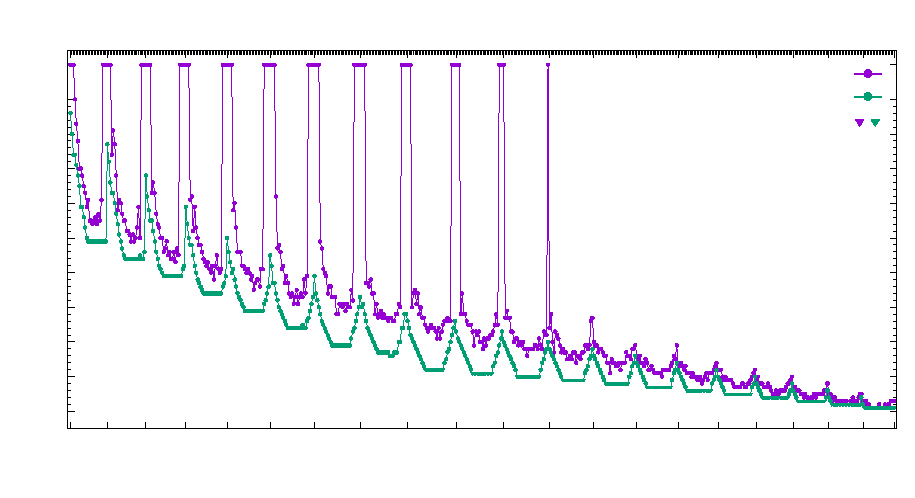
\includegraphics{resultados_5x8}}%
    \gplfronttext
  \end{picture}%
\endgroup
%
	\end{figure}
	}%
\end{frame}

\begin{frame}{Ejemplo ilustrativo en malla de $\mathsf{5\times 8}$}
	\captionsetup[figure]{belowskip = 4pt}%
	\vskip -6pt%
	\begin{figure}[H]
		\caption{Acomodo aleatorio inicial (izquierda) y acomodo encontrado por el algoritmo (derecha), mostrados en diferentes vistas.}%
		\arregloAntesDespues{caso=5x8, separacionAntesDespues=4.2, separacionVertical=0.35cm}{width=5cm}[width=5.163cm]{width=3.8cm}%
	\end{figure}
\end{frame}


\begin{frame}{Mallas de $\mathsf{7\times 7}$}
	\vfill
	\Wider[1.85cm]{
	\begin{figure}[H]
		% GNUPLOT: LaTeX picture with Postscript
\begingroup
  % Encoding inside the plot.  In the header of your document, this encoding
  % should to defined, e.g., by using
  % \usepackage[latin1,<other encodings>]{inputenc}
  \inputencoding{latin1}%
  \makeatletter
  \providecommand\color[2][]{%
    \GenericError{(gnuplot) \space\space\space\@spaces}{%
      Package color not loaded in conjunction with
      terminal option `colourtext'%
    }{See the gnuplot documentation for explanation.%
    }{Either use 'blacktext' in gnuplot or load the package
      color.sty in LaTeX.}%
    \renewcommand\color[2][]{}%
  }%
  \providecommand\includegraphics[2][]{%
    \GenericError{(gnuplot) \space\space\space\@spaces}{%
      Package graphicx or graphics not loaded%
    }{See the gnuplot documentation for explanation.%
    }{The gnuplot epslatex terminal needs graphicx.sty or graphics.sty.}%
    \renewcommand\includegraphics[2][]{}%
  }%
  \providecommand\rotatebox[2]{#2}%
  \@ifundefined{ifGPcolor}{%
    \newif\ifGPcolor
    \GPcolortrue
  }{}%
  \@ifundefined{ifGPblacktext}{%
    \newif\ifGPblacktext
    \GPblacktexttrue
  }{}%
  % define a \g@addto@macro without @ in the name:
  \let\gplgaddtomacro\g@addto@macro
  % define empty templates for all commands taking text:
  \gdef\gplbacktext{}%
  \gdef\gplfronttext{}%
  \makeatother
  \ifGPblacktext
    % no textcolor at all
    \def\colorrgb#1{}%
    \def\colorgray#1{}%
  \else
    % gray or color?
    \ifGPcolor
      \def\colorrgb#1{\color[rgb]{#1}}%
      \def\colorgray#1{\color[gray]{#1}}%
      \expandafter\def\csname LTw\endcsname{\color{white}}%
      \expandafter\def\csname LTb\endcsname{\color{black}}%
      \expandafter\def\csname LTa\endcsname{\color{black}}%
      \expandafter\def\csname LT0\endcsname{\color[rgb]{1,0,0}}%
      \expandafter\def\csname LT1\endcsname{\color[rgb]{0,1,0}}%
      \expandafter\def\csname LT2\endcsname{\color[rgb]{0,0,1}}%
      \expandafter\def\csname LT3\endcsname{\color[rgb]{1,0,1}}%
      \expandafter\def\csname LT4\endcsname{\color[rgb]{0,1,1}}%
      \expandafter\def\csname LT5\endcsname{\color[rgb]{1,1,0}}%
      \expandafter\def\csname LT6\endcsname{\color[rgb]{0,0,0}}%
      \expandafter\def\csname LT7\endcsname{\color[rgb]{1,0.3,0}}%
      \expandafter\def\csname LT8\endcsname{\color[rgb]{0.5,0.5,0.5}}%
    \else
      % gray
      \def\colorrgb#1{\color{black}}%
      \def\colorgray#1{\color[gray]{#1}}%
      \expandafter\def\csname LTw\endcsname{\color{white}}%
      \expandafter\def\csname LTb\endcsname{\color{black}}%
      \expandafter\def\csname LTa\endcsname{\color{black}}%
      \expandafter\def\csname LT0\endcsname{\color{black}}%
      \expandafter\def\csname LT1\endcsname{\color{black}}%
      \expandafter\def\csname LT2\endcsname{\color{black}}%
      \expandafter\def\csname LT3\endcsname{\color{black}}%
      \expandafter\def\csname LT4\endcsname{\color{black}}%
      \expandafter\def\csname LT5\endcsname{\color{black}}%
      \expandafter\def\csname LT6\endcsname{\color{black}}%
      \expandafter\def\csname LT7\endcsname{\color{black}}%
      \expandafter\def\csname LT8\endcsname{\color{black}}%
    \fi
  \fi
    \setlength{\unitlength}{0.0500bp}%
    \ifx\gptboxheight\undefined%
      \newlength{\gptboxheight}%
      \newlength{\gptboxwidth}%
      \newsavebox{\gptboxtext}%
    \fi%
    \setlength{\fboxrule}{0.5pt}%
    \setlength{\fboxsep}{1pt}%
\begin{picture}(8466.00,4464.00)%
    \gplgaddtomacro\gplbacktext{%
      \csname LTb\endcsname%%
      \put(448,4023){\makebox(0,0)[r]{\strut{}\raisebox{2pt}{\fontsize{9}{9}\selectfont{$\infty$}}}}%
      \put(448,726){\makebox(0,0)[r]{\strut{}\fontsize{9}{9}\selectfont{30}}}%
      \put(448,1001){\makebox(0,0)[r]{\strut{}\fontsize{9}{9}\selectfont{40}}}%
      \put(448,1275){\makebox(0,0)[r]{\strut{}\fontsize{9}{9}\selectfont{50}}}%
      \put(448,1550){\makebox(0,0)[r]{\strut{}\fontsize{9}{9}\selectfont{60}}}%
      \put(448,1825){\makebox(0,0)[r]{\strut{}\fontsize{9}{9}\selectfont{70}}}%
      \put(448,2100){\makebox(0,0)[r]{\strut{}\fontsize{9}{9}\selectfont{80}}}%
      \put(448,2374){\makebox(0,0)[r]{\strut{}\fontsize{9}{9}\selectfont{90}}}%
      \put(448,2649){\makebox(0,0)[r]{\strut{}\fontsize{9}{9}\selectfont{100}}}%
      \put(448,2924){\makebox(0,0)[r]{\strut{}\fontsize{9}{9}\selectfont{110}}}%
      \put(448,3199){\makebox(0,0)[r]{\strut{}\fontsize{9}{9}\selectfont{120}}}%
      \put(448,3474){\makebox(0,0)[r]{\strut{}\fontsize{9}{9}\selectfont{130}}}%
      \put(448,3748){\makebox(0,0)[r]{\strut{}\fontsize{9}{9}\selectfont{140}}}%
      \put(375,308){\rotatebox{30}{\makebox(0,0)[l]{\strut{}\fontsize{7.6}{7.6}\selectfont{40,9}}}}%
      \put(679,308){\rotatebox{30}{\makebox(0,0)[l]{\strut{}\fontsize{7.6}{7.6}\selectfont{40,8}}}}%
      \put(993,308){\rotatebox{30}{\makebox(0,0)[l]{\strut{}\fontsize{7.6}{7.6}\selectfont{40,7}}}}%
      \put(1317,308){\rotatebox{30}{\makebox(0,0)[l]{\strut{}\fontsize{7.6}{7.6}\selectfont{40,6}}}}%
      \put(1650,308){\rotatebox{30}{\makebox(0,0)[l]{\strut{}\fontsize{7.6}{7.6}\selectfont{40,5}}}}%
      \put(1992,308){\rotatebox{30}{\makebox(0,0)[l]{\strut{}\fontsize{7.6}{7.6}\selectfont{40,4}}}}%
      \put(2344,308){\rotatebox{30}{\makebox(0,0)[l]{\strut{}\fontsize{7.6}{7.6}\selectfont{40,3}}}}%
      \put(2706,308){\rotatebox{30}{\makebox(0,0)[l]{\strut{}\fontsize{7.6}{7.6}\selectfont{40,2}}}}%
      \put(3077,308){\rotatebox{30}{\makebox(0,0)[l]{\strut{}\fontsize{7.6}{7.6}\selectfont{40,1}}}}%
      \put(3457,308){\rotatebox{30}{\makebox(0,0)[l]{\strut{}\fontsize{7.6}{7.6}\selectfont{40,0}}}}%
      \put(3848,308){\rotatebox{30}{\makebox(0,0)[l]{\strut{}\fontsize{7.6}{7.6}\selectfont{39,0}}}}%
      \put(4228,308){\rotatebox{30}{\makebox(0,0)[l]{\strut{}\fontsize{7.6}{7.6}\selectfont{38,0}}}}%
      \put(4599,308){\rotatebox{30}{\makebox(0,0)[l]{\strut{}\fontsize{7.6}{7.6}\selectfont{37,0}}}}%
      \put(4961,308){\rotatebox{30}{\makebox(0,0)[l]{\strut{}\fontsize{7.6}{7.6}\selectfont{36,0}}}}%
      \put(5313,308){\rotatebox{30}{\makebox(0,0)[l]{\strut{}\fontsize{7.6}{7.6}\selectfont{35,0}}}}%
      \put(5655,308){\rotatebox{30}{\makebox(0,0)[l]{\strut{}\fontsize{7.6}{7.6}\selectfont{34,0}}}}%
      \put(5988,308){\rotatebox{30}{\makebox(0,0)[l]{\strut{}\fontsize{7.6}{7.6}\selectfont{33,0}}}}%
      \put(6312,308){\rotatebox{30}{\makebox(0,0)[l]{\strut{}\fontsize{7.6}{7.6}\selectfont{32,0}}}}%
      \put(6626,308){\rotatebox{30}{\makebox(0,0)[l]{\strut{}\fontsize{7.6}{7.6}\selectfont{31,0}}}}%
      \put(6930,308){\rotatebox{30}{\makebox(0,0)[l]{\strut{}\fontsize{7.6}{7.6}\selectfont{30,0}}}}%
      \put(7225,308){\rotatebox{30}{\makebox(0,0)[l]{\strut{}\fontsize{7.6}{7.6}\selectfont{29,0}}}}%
      \put(7510,308){\rotatebox{30}{\makebox(0,0)[l]{\strut{}\fontsize{7.6}{7.6}\selectfont{28,0}}}}%
      \put(7786,308){\rotatebox{30}{\makebox(0,0)[l]{\strut{}\fontsize{7.6}{7.6}\selectfont{27,0}}}}%
      \put(8053,308){\rotatebox{30}{\makebox(0,0)[l]{\strut{}\fontsize{7.6}{7.6}\selectfont{26,0}}}}%
      \put(8300,308){\rotatebox{30}{\makebox(0,0)[l]{\strut{}\fontsize{7.6}{7.6}\selectfont{0,26}}}}%
      \put(443,4144){\rotatebox{90}{\makebox(0,0)[l]{\strut{}\fontsize{0.2}{0.2}\selectfont{39,10}}}}%
      \put(452,4144){\rotatebox{90}{\makebox(0,0)[l]{\strut{}\fontsize{0.2}{0.2}\selectfont{38,11}}}}%
      \put(462,4144){\rotatebox{90}{\makebox(0,0)[l]{\strut{}\fontsize{0.2}{0.2}\selectfont{37,12}}}}%
      \put(471,4144){\rotatebox{90}{\makebox(0,0)[l]{\strut{}\fontsize{0.2}{0.2}\selectfont{36,13}}}}%
      \put(481,4144){\rotatebox{90}{\makebox(0,0)[l]{\strut{}\fontsize{0.2}{0.2}\selectfont{35,14}}}}%
      \put(490,4144){\rotatebox{90}{\makebox(0,0)[l]{\strut{}\fontsize{0.2}{0.2}\selectfont{34,15}}}}%
      \put(500,4144){\rotatebox{90}{\makebox(0,0)[l]{\strut{}\fontsize{0.2}{0.2}\selectfont{33,16}}}}%
      \put(509,4144){\rotatebox{90}{\makebox(0,0)[l]{\strut{}\fontsize{0.2}{0.2}\selectfont{32,17}}}}%
      \put(519,4144){\rotatebox{90}{\makebox(0,0)[l]{\strut{}\fontsize{0.2}{0.2}\selectfont{31,18}}}}%
      \put(528,4144){\rotatebox{90}{\makebox(0,0)[l]{\strut{}\fontsize{0.2}{0.2}\selectfont{30,19}}}}%
      \put(538,4144){\rotatebox{90}{\makebox(0,0)[l]{\strut{}\fontsize{0.2}{0.2}\selectfont{29,20}}}}%
      \put(547,4144){\rotatebox{90}{\makebox(0,0)[l]{\strut{}\fontsize{0.2}{0.2}\selectfont{28,21}}}}%
      \put(557,4144){\rotatebox{90}{\makebox(0,0)[l]{\strut{}\fontsize{0.2}{0.2}\selectfont{27,22}}}}%
      \put(566,4144){\rotatebox{90}{\makebox(0,0)[l]{\strut{}\fontsize{0.2}{0.2}\selectfont{26,23}}}}%
      \put(576,4144){\rotatebox{90}{\makebox(0,0)[l]{\strut{}\fontsize{0.2}{0.2}\selectfont{25,24}}}}%
      \put(585,4144){\rotatebox{90}{\makebox(0,0)[l]{\strut{}\fontsize{0.2}{0.2}\selectfont{24,25}}}}%
      \put(595,4144){\rotatebox{90}{\makebox(0,0)[l]{\strut{}\fontsize{0.2}{0.2}\selectfont{23,26}}}}%
      \put(604,4144){\rotatebox{90}{\makebox(0,0)[l]{\strut{}\fontsize{0.2}{0.2}\selectfont{22,27}}}}%
      \put(614,4144){\rotatebox{90}{\makebox(0,0)[l]{\strut{}\fontsize{0.2}{0.2}\selectfont{21,28}}}}%
      \put(623,4144){\rotatebox{90}{\makebox(0,0)[l]{\strut{}\fontsize{0.2}{0.2}\selectfont{20,29}}}}%
      \put(633,4144){\rotatebox{90}{\makebox(0,0)[l]{\strut{}\fontsize{0.2}{0.2}\selectfont{19,30}}}}%
      \put(642,4144){\rotatebox{90}{\makebox(0,0)[l]{\strut{}\fontsize{0.2}{0.2}\selectfont{18,31}}}}%
      \put(652,4144){\rotatebox{90}{\makebox(0,0)[l]{\strut{}\fontsize{0.2}{0.2}\selectfont{17,32}}}}%
      \put(661,4144){\rotatebox{90}{\makebox(0,0)[l]{\strut{}\fontsize{0.2}{0.2}\selectfont{16,33}}}}%
      \put(671,4144){\rotatebox{90}{\makebox(0,0)[l]{\strut{}\fontsize{0.2}{0.2}\selectfont{15,34}}}}%
      \put(680,4144){\rotatebox{90}{\makebox(0,0)[l]{\strut{}\fontsize{0.2}{0.2}\selectfont{14,35}}}}%
      \put(690,4144){\rotatebox{90}{\makebox(0,0)[l]{\strut{}\fontsize{0.2}{0.2}\selectfont{13,36}}}}%
      \put(699,4144){\rotatebox{90}{\makebox(0,0)[l]{\strut{}\fontsize{0.2}{0.2}\selectfont{12,37}}}}%
      \put(709,4144){\rotatebox{90}{\makebox(0,0)[l]{\strut{}\fontsize{0.2}{0.2}\selectfont{11,38}}}}%
      \put(718,4144){\rotatebox{90}{\makebox(0,0)[l]{\strut{}\fontsize{0.2}{0.2}\selectfont{10,39}}}}%
      \put(728,4144){\rotatebox{90}{\makebox(0,0)[l]{\strut{}\fontsize{0.2}{0.2}\selectfont{9,40}}}}%
      \put(747,4144){\rotatebox{90}{\makebox(0,0)[l]{\strut{}\fontsize{0.2}{0.2}\selectfont{39,9}}}}%
      \put(756,4144){\rotatebox{90}{\makebox(0,0)[l]{\strut{}\fontsize{0.2}{0.2}\selectfont{38,10}}}}%
      \put(766,4144){\rotatebox{90}{\makebox(0,0)[l]{\strut{}\fontsize{0.2}{0.2}\selectfont{37,11}}}}%
      \put(776,4144){\rotatebox{90}{\makebox(0,0)[l]{\strut{}\fontsize{0.2}{0.2}\selectfont{36,12}}}}%
      \put(785,4144){\rotatebox{90}{\makebox(0,0)[l]{\strut{}\fontsize{0.2}{0.2}\selectfont{35,13}}}}%
      \put(795,4144){\rotatebox{90}{\makebox(0,0)[l]{\strut{}\fontsize{0.2}{0.2}\selectfont{34,14}}}}%
      \put(804,4144){\rotatebox{90}{\makebox(0,0)[l]{\strut{}\fontsize{0.2}{0.2}\selectfont{33,15}}}}%
      \put(814,4144){\rotatebox{90}{\makebox(0,0)[l]{\strut{}\fontsize{0.2}{0.2}\selectfont{32,16}}}}%
      \put(823,4144){\rotatebox{90}{\makebox(0,0)[l]{\strut{}\fontsize{0.2}{0.2}\selectfont{31,17}}}}%
      \put(833,4144){\rotatebox{90}{\makebox(0,0)[l]{\strut{}\fontsize{0.2}{0.2}\selectfont{30,18}}}}%
      \put(842,4144){\rotatebox{90}{\makebox(0,0)[l]{\strut{}\fontsize{0.2}{0.2}\selectfont{29,19}}}}%
      \put(852,4144){\rotatebox{90}{\makebox(0,0)[l]{\strut{}\fontsize{0.2}{0.2}\selectfont{28,20}}}}%
      \put(861,4144){\rotatebox{90}{\makebox(0,0)[l]{\strut{}\fontsize{0.2}{0.2}\selectfont{27,21}}}}%
      \put(871,4144){\rotatebox{90}{\makebox(0,0)[l]{\strut{}\fontsize{0.2}{0.2}\selectfont{26,22}}}}%
      \put(880,4144){\rotatebox{90}{\makebox(0,0)[l]{\strut{}\fontsize{0.2}{0.2}\selectfont{25,23}}}}%
      \put(890,4144){\rotatebox{90}{\makebox(0,0)[l]{\strut{}\fontsize{0.2}{0.2}\selectfont{24,24}}}}%
      \put(899,4144){\rotatebox{90}{\makebox(0,0)[l]{\strut{}\fontsize{0.2}{0.2}\selectfont{23,25}}}}%
      \put(909,4144){\rotatebox{90}{\makebox(0,0)[l]{\strut{}\fontsize{0.2}{0.2}\selectfont{22,26}}}}%
      \put(918,4144){\rotatebox{90}{\makebox(0,0)[l]{\strut{}\fontsize{0.2}{0.2}\selectfont{21,27}}}}%
      \put(928,4144){\rotatebox{90}{\makebox(0,0)[l]{\strut{}\fontsize{0.2}{0.2}\selectfont{20,28}}}}%
      \put(937,4144){\rotatebox{90}{\makebox(0,0)[l]{\strut{}\fontsize{0.2}{0.2}\selectfont{19,29}}}}%
      \put(947,4144){\rotatebox{90}{\makebox(0,0)[l]{\strut{}\fontsize{0.2}{0.2}\selectfont{18,30}}}}%
      \put(956,4144){\rotatebox{90}{\makebox(0,0)[l]{\strut{}\fontsize{0.2}{0.2}\selectfont{17,31}}}}%
      \put(966,4144){\rotatebox{90}{\makebox(0,0)[l]{\strut{}\fontsize{0.2}{0.2}\selectfont{16,32}}}}%
      \put(975,4144){\rotatebox{90}{\makebox(0,0)[l]{\strut{}\fontsize{0.2}{0.2}\selectfont{15,33}}}}%
      \put(985,4144){\rotatebox{90}{\makebox(0,0)[l]{\strut{}\fontsize{0.2}{0.2}\selectfont{14,34}}}}%
      \put(994,4144){\rotatebox{90}{\makebox(0,0)[l]{\strut{}\fontsize{0.2}{0.2}\selectfont{13,35}}}}%
      \put(1004,4144){\rotatebox{90}{\makebox(0,0)[l]{\strut{}\fontsize{0.2}{0.2}\selectfont{12,36}}}}%
      \put(1013,4144){\rotatebox{90}{\makebox(0,0)[l]{\strut{}\fontsize{0.2}{0.2}\selectfont{11,37}}}}%
      \put(1023,4144){\rotatebox{90}{\makebox(0,0)[l]{\strut{}\fontsize{0.2}{0.2}\selectfont{10,38}}}}%
      \put(1032,4144){\rotatebox{90}{\makebox(0,0)[l]{\strut{}\fontsize{0.2}{0.2}\selectfont{9,39}}}}%
      \put(1042,4144){\rotatebox{90}{\makebox(0,0)[l]{\strut{}\fontsize{0.2}{0.2}\selectfont{8,40}}}}%
      \put(1061,4144){\rotatebox{90}{\makebox(0,0)[l]{\strut{}\fontsize{0.2}{0.2}\selectfont{39,8}}}}%
      \put(1070,4144){\rotatebox{90}{\makebox(0,0)[l]{\strut{}\fontsize{0.2}{0.2}\selectfont{38,9}}}}%
      \put(1080,4144){\rotatebox{90}{\makebox(0,0)[l]{\strut{}\fontsize{0.2}{0.2}\selectfont{37,10}}}}%
      \put(1089,4144){\rotatebox{90}{\makebox(0,0)[l]{\strut{}\fontsize{0.2}{0.2}\selectfont{36,11}}}}%
      \put(1099,4144){\rotatebox{90}{\makebox(0,0)[l]{\strut{}\fontsize{0.2}{0.2}\selectfont{35,12}}}}%
      \put(1109,4144){\rotatebox{90}{\makebox(0,0)[l]{\strut{}\fontsize{0.2}{0.2}\selectfont{34,13}}}}%
      \put(1118,4144){\rotatebox{90}{\makebox(0,0)[l]{\strut{}\fontsize{0.2}{0.2}\selectfont{33,14}}}}%
      \put(1128,4144){\rotatebox{90}{\makebox(0,0)[l]{\strut{}\fontsize{0.2}{0.2}\selectfont{32,15}}}}%
      \put(1137,4144){\rotatebox{90}{\makebox(0,0)[l]{\strut{}\fontsize{0.2}{0.2}\selectfont{31,16}}}}%
      \put(1147,4144){\rotatebox{90}{\makebox(0,0)[l]{\strut{}\fontsize{0.2}{0.2}\selectfont{30,17}}}}%
      \put(1156,4144){\rotatebox{90}{\makebox(0,0)[l]{\strut{}\fontsize{0.2}{0.2}\selectfont{29,18}}}}%
      \put(1166,4144){\rotatebox{90}{\makebox(0,0)[l]{\strut{}\fontsize{0.2}{0.2}\selectfont{28,19}}}}%
      \put(1175,4144){\rotatebox{90}{\makebox(0,0)[l]{\strut{}\fontsize{0.2}{0.2}\selectfont{27,20}}}}%
      \put(1185,4144){\rotatebox{90}{\makebox(0,0)[l]{\strut{}\fontsize{0.2}{0.2}\selectfont{26,21}}}}%
      \put(1194,4144){\rotatebox{90}{\makebox(0,0)[l]{\strut{}\fontsize{0.2}{0.2}\selectfont{25,22}}}}%
      \put(1204,4144){\rotatebox{90}{\makebox(0,0)[l]{\strut{}\fontsize{0.2}{0.2}\selectfont{24,23}}}}%
      \put(1213,4144){\rotatebox{90}{\makebox(0,0)[l]{\strut{}\fontsize{0.2}{0.2}\selectfont{23,24}}}}%
      \put(1223,4144){\rotatebox{90}{\makebox(0,0)[l]{\strut{}\fontsize{0.2}{0.2}\selectfont{22,25}}}}%
      \put(1232,4144){\rotatebox{90}{\makebox(0,0)[l]{\strut{}\fontsize{0.2}{0.2}\selectfont{21,26}}}}%
      \put(1242,4144){\rotatebox{90}{\makebox(0,0)[l]{\strut{}\fontsize{0.2}{0.2}\selectfont{20,27}}}}%
      \put(1251,4144){\rotatebox{90}{\makebox(0,0)[l]{\strut{}\fontsize{0.2}{0.2}\selectfont{19,28}}}}%
      \put(1261,4144){\rotatebox{90}{\makebox(0,0)[l]{\strut{}\fontsize{0.2}{0.2}\selectfont{18,29}}}}%
      \put(1270,4144){\rotatebox{90}{\makebox(0,0)[l]{\strut{}\fontsize{0.2}{0.2}\selectfont{17,30}}}}%
      \put(1280,4144){\rotatebox{90}{\makebox(0,0)[l]{\strut{}\fontsize{0.2}{0.2}\selectfont{16,31}}}}%
      \put(1289,4144){\rotatebox{90}{\makebox(0,0)[l]{\strut{}\fontsize{0.2}{0.2}\selectfont{15,32}}}}%
      \put(1299,4144){\rotatebox{90}{\makebox(0,0)[l]{\strut{}\fontsize{0.2}{0.2}\selectfont{14,33}}}}%
      \put(1308,4144){\rotatebox{90}{\makebox(0,0)[l]{\strut{}\fontsize{0.2}{0.2}\selectfont{13,34}}}}%
      \put(1318,4144){\rotatebox{90}{\makebox(0,0)[l]{\strut{}\fontsize{0.2}{0.2}\selectfont{12,35}}}}%
      \put(1327,4144){\rotatebox{90}{\makebox(0,0)[l]{\strut{}\fontsize{0.2}{0.2}\selectfont{11,36}}}}%
      \put(1337,4144){\rotatebox{90}{\makebox(0,0)[l]{\strut{}\fontsize{0.2}{0.2}\selectfont{10,37}}}}%
      \put(1346,4144){\rotatebox{90}{\makebox(0,0)[l]{\strut{}\fontsize{0.2}{0.2}\selectfont{9,38}}}}%
      \put(1356,4144){\rotatebox{90}{\makebox(0,0)[l]{\strut{}\fontsize{0.2}{0.2}\selectfont{8,39}}}}%
      \put(1365,4144){\rotatebox{90}{\makebox(0,0)[l]{\strut{}\fontsize{0.2}{0.2}\selectfont{7,40}}}}%
      \put(1384,4144){\rotatebox{90}{\makebox(0,0)[l]{\strut{}\fontsize{0.2}{0.2}\selectfont{39,7}}}}%
      \put(1394,4144){\rotatebox{90}{\makebox(0,0)[l]{\strut{}\fontsize{0.2}{0.2}\selectfont{38,8}}}}%
      \put(1403,4144){\rotatebox{90}{\makebox(0,0)[l]{\strut{}\fontsize{0.2}{0.2}\selectfont{37,9}}}}%
      \put(1413,4144){\rotatebox{90}{\makebox(0,0)[l]{\strut{}\fontsize{0.2}{0.2}\selectfont{36,10}}}}%
      \put(1422,4144){\rotatebox{90}{\makebox(0,0)[l]{\strut{}\fontsize{0.2}{0.2}\selectfont{35,11}}}}%
      \put(1432,4144){\rotatebox{90}{\makebox(0,0)[l]{\strut{}\fontsize{0.2}{0.2}\selectfont{34,12}}}}%
      \put(1441,4144){\rotatebox{90}{\makebox(0,0)[l]{\strut{}\fontsize{0.2}{0.2}\selectfont{33,13}}}}%
      \put(1451,4144){\rotatebox{90}{\makebox(0,0)[l]{\strut{}\fontsize{0.2}{0.2}\selectfont{32,14}}}}%
      \put(1461,4144){\rotatebox{90}{\makebox(0,0)[l]{\strut{}\fontsize{0.2}{0.2}\selectfont{31,15}}}}%
      \put(1470,4144){\rotatebox{90}{\makebox(0,0)[l]{\strut{}\fontsize{0.2}{0.2}\selectfont{30,16}}}}%
      \put(1480,4144){\rotatebox{90}{\makebox(0,0)[l]{\strut{}\fontsize{0.2}{0.2}\selectfont{29,17}}}}%
      \put(1489,4144){\rotatebox{90}{\makebox(0,0)[l]{\strut{}\fontsize{0.2}{0.2}\selectfont{28,18}}}}%
      \put(1499,4144){\rotatebox{90}{\makebox(0,0)[l]{\strut{}\fontsize{0.2}{0.2}\selectfont{27,19}}}}%
      \put(1508,4144){\rotatebox{90}{\makebox(0,0)[l]{\strut{}\fontsize{0.2}{0.2}\selectfont{26,20}}}}%
      \put(1518,4144){\rotatebox{90}{\makebox(0,0)[l]{\strut{}\fontsize{0.2}{0.2}\selectfont{25,21}}}}%
      \put(1527,4144){\rotatebox{90}{\makebox(0,0)[l]{\strut{}\fontsize{0.2}{0.2}\selectfont{24,22}}}}%
      \put(1537,4144){\rotatebox{90}{\makebox(0,0)[l]{\strut{}\fontsize{0.2}{0.2}\selectfont{23,23}}}}%
      \put(1546,4144){\rotatebox{90}{\makebox(0,0)[l]{\strut{}\fontsize{0.2}{0.2}\selectfont{22,24}}}}%
      \put(1556,4144){\rotatebox{90}{\makebox(0,0)[l]{\strut{}\fontsize{0.2}{0.2}\selectfont{21,25}}}}%
      \put(1565,4144){\rotatebox{90}{\makebox(0,0)[l]{\strut{}\fontsize{0.2}{0.2}\selectfont{20,26}}}}%
      \put(1575,4144){\rotatebox{90}{\makebox(0,0)[l]{\strut{}\fontsize{0.2}{0.2}\selectfont{19,27}}}}%
      \put(1584,4144){\rotatebox{90}{\makebox(0,0)[l]{\strut{}\fontsize{0.2}{0.2}\selectfont{18,28}}}}%
      \put(1594,4144){\rotatebox{90}{\makebox(0,0)[l]{\strut{}\fontsize{0.2}{0.2}\selectfont{17,29}}}}%
      \put(1603,4144){\rotatebox{90}{\makebox(0,0)[l]{\strut{}\fontsize{0.2}{0.2}\selectfont{16,30}}}}%
      \put(1613,4144){\rotatebox{90}{\makebox(0,0)[l]{\strut{}\fontsize{0.2}{0.2}\selectfont{15,31}}}}%
      \put(1622,4144){\rotatebox{90}{\makebox(0,0)[l]{\strut{}\fontsize{0.2}{0.2}\selectfont{14,32}}}}%
      \put(1632,4144){\rotatebox{90}{\makebox(0,0)[l]{\strut{}\fontsize{0.2}{0.2}\selectfont{13,33}}}}%
      \put(1641,4144){\rotatebox{90}{\makebox(0,0)[l]{\strut{}\fontsize{0.2}{0.2}\selectfont{12,34}}}}%
      \put(1651,4144){\rotatebox{90}{\makebox(0,0)[l]{\strut{}\fontsize{0.2}{0.2}\selectfont{11,35}}}}%
      \put(1660,4144){\rotatebox{90}{\makebox(0,0)[l]{\strut{}\fontsize{0.2}{0.2}\selectfont{10,36}}}}%
      \put(1670,4144){\rotatebox{90}{\makebox(0,0)[l]{\strut{}\fontsize{0.2}{0.2}\selectfont{9,37}}}}%
      \put(1679,4144){\rotatebox{90}{\makebox(0,0)[l]{\strut{}\fontsize{0.2}{0.2}\selectfont{8,38}}}}%
      \put(1689,4144){\rotatebox{90}{\makebox(0,0)[l]{\strut{}\fontsize{0.2}{0.2}\selectfont{7,39}}}}%
      \put(1698,4144){\rotatebox{90}{\makebox(0,0)[l]{\strut{}\fontsize{0.2}{0.2}\selectfont{6,40}}}}%
      \put(1717,4144){\rotatebox{90}{\makebox(0,0)[l]{\strut{}\fontsize{0.2}{0.2}\selectfont{39,6}}}}%
      \put(1727,4144){\rotatebox{90}{\makebox(0,0)[l]{\strut{}\fontsize{0.2}{0.2}\selectfont{38,7}}}}%
      \put(1736,4144){\rotatebox{90}{\makebox(0,0)[l]{\strut{}\fontsize{0.2}{0.2}\selectfont{37,8}}}}%
      \put(1746,4144){\rotatebox{90}{\makebox(0,0)[l]{\strut{}\fontsize{0.2}{0.2}\selectfont{36,9}}}}%
      \put(1755,4144){\rotatebox{90}{\makebox(0,0)[l]{\strut{}\fontsize{0.2}{0.2}\selectfont{35,10}}}}%
      \put(1765,4144){\rotatebox{90}{\makebox(0,0)[l]{\strut{}\fontsize{0.2}{0.2}\selectfont{34,11}}}}%
      \put(1774,4144){\rotatebox{90}{\makebox(0,0)[l]{\strut{}\fontsize{0.2}{0.2}\selectfont{33,12}}}}%
      \put(1784,4144){\rotatebox{90}{\makebox(0,0)[l]{\strut{}\fontsize{0.2}{0.2}\selectfont{32,13}}}}%
      \put(1793,4144){\rotatebox{90}{\makebox(0,0)[l]{\strut{}\fontsize{0.2}{0.2}\selectfont{31,14}}}}%
      \put(1803,4144){\rotatebox{90}{\makebox(0,0)[l]{\strut{}\fontsize{0.2}{0.2}\selectfont{30,15}}}}%
      \put(1813,4144){\rotatebox{90}{\makebox(0,0)[l]{\strut{}\fontsize{0.2}{0.2}\selectfont{29,16}}}}%
      \put(1822,4144){\rotatebox{90}{\makebox(0,0)[l]{\strut{}\fontsize{0.2}{0.2}\selectfont{28,17}}}}%
      \put(1832,4144){\rotatebox{90}{\makebox(0,0)[l]{\strut{}\fontsize{0.2}{0.2}\selectfont{27,18}}}}%
      \put(1841,4144){\rotatebox{90}{\makebox(0,0)[l]{\strut{}\fontsize{0.2}{0.2}\selectfont{26,19}}}}%
      \put(1851,4144){\rotatebox{90}{\makebox(0,0)[l]{\strut{}\fontsize{0.2}{0.2}\selectfont{25,20}}}}%
      \put(1860,4144){\rotatebox{90}{\makebox(0,0)[l]{\strut{}\fontsize{0.2}{0.2}\selectfont{24,21}}}}%
      \put(1870,4144){\rotatebox{90}{\makebox(0,0)[l]{\strut{}\fontsize{0.2}{0.2}\selectfont{23,22}}}}%
      \put(1879,4144){\rotatebox{90}{\makebox(0,0)[l]{\strut{}\fontsize{0.2}{0.2}\selectfont{22,23}}}}%
      \put(1889,4144){\rotatebox{90}{\makebox(0,0)[l]{\strut{}\fontsize{0.2}{0.2}\selectfont{21,24}}}}%
      \put(1898,4144){\rotatebox{90}{\makebox(0,0)[l]{\strut{}\fontsize{0.2}{0.2}\selectfont{20,25}}}}%
      \put(1908,4144){\rotatebox{90}{\makebox(0,0)[l]{\strut{}\fontsize{0.2}{0.2}\selectfont{19,26}}}}%
      \put(1917,4144){\rotatebox{90}{\makebox(0,0)[l]{\strut{}\fontsize{0.2}{0.2}\selectfont{18,27}}}}%
      \put(1927,4144){\rotatebox{90}{\makebox(0,0)[l]{\strut{}\fontsize{0.2}{0.2}\selectfont{17,28}}}}%
      \put(1936,4144){\rotatebox{90}{\makebox(0,0)[l]{\strut{}\fontsize{0.2}{0.2}\selectfont{16,29}}}}%
      \put(1946,4144){\rotatebox{90}{\makebox(0,0)[l]{\strut{}\fontsize{0.2}{0.2}\selectfont{15,30}}}}%
      \put(1955,4144){\rotatebox{90}{\makebox(0,0)[l]{\strut{}\fontsize{0.2}{0.2}\selectfont{14,31}}}}%
      \put(1965,4144){\rotatebox{90}{\makebox(0,0)[l]{\strut{}\fontsize{0.2}{0.2}\selectfont{13,32}}}}%
      \put(1974,4144){\rotatebox{90}{\makebox(0,0)[l]{\strut{}\fontsize{0.2}{0.2}\selectfont{12,33}}}}%
      \put(1984,4144){\rotatebox{90}{\makebox(0,0)[l]{\strut{}\fontsize{0.2}{0.2}\selectfont{11,34}}}}%
      \put(1993,4144){\rotatebox{90}{\makebox(0,0)[l]{\strut{}\fontsize{0.2}{0.2}\selectfont{10,35}}}}%
      \put(2003,4144){\rotatebox{90}{\makebox(0,0)[l]{\strut{}\fontsize{0.2}{0.2}\selectfont{9,36}}}}%
      \put(2012,4144){\rotatebox{90}{\makebox(0,0)[l]{\strut{}\fontsize{0.2}{0.2}\selectfont{8,37}}}}%
      \put(2022,4144){\rotatebox{90}{\makebox(0,0)[l]{\strut{}\fontsize{0.2}{0.2}\selectfont{7,38}}}}%
      \put(2031,4144){\rotatebox{90}{\makebox(0,0)[l]{\strut{}\fontsize{0.2}{0.2}\selectfont{6,39}}}}%
      \put(2041,4144){\rotatebox{90}{\makebox(0,0)[l]{\strut{}\fontsize{0.2}{0.2}\selectfont{5,40}}}}%
      \put(2060,4144){\rotatebox{90}{\makebox(0,0)[l]{\strut{}\fontsize{0.2}{0.2}\selectfont{39,5}}}}%
      \put(2069,4144){\rotatebox{90}{\makebox(0,0)[l]{\strut{}\fontsize{0.2}{0.2}\selectfont{38,6}}}}%
      \put(2079,4144){\rotatebox{90}{\makebox(0,0)[l]{\strut{}\fontsize{0.2}{0.2}\selectfont{37,7}}}}%
      \put(2088,4144){\rotatebox{90}{\makebox(0,0)[l]{\strut{}\fontsize{0.2}{0.2}\selectfont{36,8}}}}%
      \put(2098,4144){\rotatebox{90}{\makebox(0,0)[l]{\strut{}\fontsize{0.2}{0.2}\selectfont{35,9}}}}%
      \put(2107,4144){\rotatebox{90}{\makebox(0,0)[l]{\strut{}\fontsize{0.2}{0.2}\selectfont{34,10}}}}%
      \put(2117,4144){\rotatebox{90}{\makebox(0,0)[l]{\strut{}\fontsize{0.2}{0.2}\selectfont{33,11}}}}%
      \put(2126,4144){\rotatebox{90}{\makebox(0,0)[l]{\strut{}\fontsize{0.2}{0.2}\selectfont{32,12}}}}%
      \put(2136,4144){\rotatebox{90}{\makebox(0,0)[l]{\strut{}\fontsize{0.2}{0.2}\selectfont{31,13}}}}%
      \put(2146,4144){\rotatebox{90}{\makebox(0,0)[l]{\strut{}\fontsize{0.2}{0.2}\selectfont{30,14}}}}%
      \put(2155,4144){\rotatebox{90}{\makebox(0,0)[l]{\strut{}\fontsize{0.2}{0.2}\selectfont{29,15}}}}%
      \put(2165,4144){\rotatebox{90}{\makebox(0,0)[l]{\strut{}\fontsize{0.2}{0.2}\selectfont{28,16}}}}%
      \put(2174,4144){\rotatebox{90}{\makebox(0,0)[l]{\strut{}\fontsize{0.2}{0.2}\selectfont{27,17}}}}%
      \put(2184,4144){\rotatebox{90}{\makebox(0,0)[l]{\strut{}\fontsize{0.2}{0.2}\selectfont{26,18}}}}%
      \put(2193,4144){\rotatebox{90}{\makebox(0,0)[l]{\strut{}\fontsize{0.2}{0.2}\selectfont{25,19}}}}%
      \put(2203,4144){\rotatebox{90}{\makebox(0,0)[l]{\strut{}\fontsize{0.2}{0.2}\selectfont{24,20}}}}%
      \put(2212,4144){\rotatebox{90}{\makebox(0,0)[l]{\strut{}\fontsize{0.2}{0.2}\selectfont{23,21}}}}%
      \put(2222,4144){\rotatebox{90}{\makebox(0,0)[l]{\strut{}\fontsize{0.2}{0.2}\selectfont{22,22}}}}%
      \put(2231,4144){\rotatebox{90}{\makebox(0,0)[l]{\strut{}\fontsize{0.2}{0.2}\selectfont{21,23}}}}%
      \put(2241,4144){\rotatebox{90}{\makebox(0,0)[l]{\strut{}\fontsize{0.2}{0.2}\selectfont{20,24}}}}%
      \put(2250,4144){\rotatebox{90}{\makebox(0,0)[l]{\strut{}\fontsize{0.2}{0.2}\selectfont{19,25}}}}%
      \put(2260,4144){\rotatebox{90}{\makebox(0,0)[l]{\strut{}\fontsize{0.2}{0.2}\selectfont{18,26}}}}%
      \put(2269,4144){\rotatebox{90}{\makebox(0,0)[l]{\strut{}\fontsize{0.2}{0.2}\selectfont{17,27}}}}%
      \put(2279,4144){\rotatebox{90}{\makebox(0,0)[l]{\strut{}\fontsize{0.2}{0.2}\selectfont{16,28}}}}%
      \put(2288,4144){\rotatebox{90}{\makebox(0,0)[l]{\strut{}\fontsize{0.2}{0.2}\selectfont{15,29}}}}%
      \put(2298,4144){\rotatebox{90}{\makebox(0,0)[l]{\strut{}\fontsize{0.2}{0.2}\selectfont{14,30}}}}%
      \put(2307,4144){\rotatebox{90}{\makebox(0,0)[l]{\strut{}\fontsize{0.2}{0.2}\selectfont{13,31}}}}%
      \put(2317,4144){\rotatebox{90}{\makebox(0,0)[l]{\strut{}\fontsize{0.2}{0.2}\selectfont{12,32}}}}%
      \put(2326,4144){\rotatebox{90}{\makebox(0,0)[l]{\strut{}\fontsize{0.2}{0.2}\selectfont{11,33}}}}%
      \put(2336,4144){\rotatebox{90}{\makebox(0,0)[l]{\strut{}\fontsize{0.2}{0.2}\selectfont{10,34}}}}%
      \put(2345,4144){\rotatebox{90}{\makebox(0,0)[l]{\strut{}\fontsize{0.2}{0.2}\selectfont{9,35}}}}%
      \put(2355,4144){\rotatebox{90}{\makebox(0,0)[l]{\strut{}\fontsize{0.2}{0.2}\selectfont{8,36}}}}%
      \put(2364,4144){\rotatebox{90}{\makebox(0,0)[l]{\strut{}\fontsize{0.2}{0.2}\selectfont{7,37}}}}%
      \put(2374,4144){\rotatebox{90}{\makebox(0,0)[l]{\strut{}\fontsize{0.2}{0.2}\selectfont{6,38}}}}%
      \put(2383,4144){\rotatebox{90}{\makebox(0,0)[l]{\strut{}\fontsize{0.2}{0.2}\selectfont{5,39}}}}%
      \put(2393,4144){\rotatebox{90}{\makebox(0,0)[l]{\strut{}\fontsize{0.2}{0.2}\selectfont{4,40}}}}%
      \put(2412,4144){\rotatebox{90}{\makebox(0,0)[l]{\strut{}\fontsize{0.2}{0.2}\selectfont{39,4}}}}%
      \put(2421,4144){\rotatebox{90}{\makebox(0,0)[l]{\strut{}\fontsize{0.2}{0.2}\selectfont{38,5}}}}%
      \put(2431,4144){\rotatebox{90}{\makebox(0,0)[l]{\strut{}\fontsize{0.2}{0.2}\selectfont{37,6}}}}%
      \put(2440,4144){\rotatebox{90}{\makebox(0,0)[l]{\strut{}\fontsize{0.2}{0.2}\selectfont{36,7}}}}%
      \put(2450,4144){\rotatebox{90}{\makebox(0,0)[l]{\strut{}\fontsize{0.2}{0.2}\selectfont{35,8}}}}%
      \put(2459,4144){\rotatebox{90}{\makebox(0,0)[l]{\strut{}\fontsize{0.2}{0.2}\selectfont{34,9}}}}%
      \put(2469,4144){\rotatebox{90}{\makebox(0,0)[l]{\strut{}\fontsize{0.2}{0.2}\selectfont{33,10}}}}%
      \put(2478,4144){\rotatebox{90}{\makebox(0,0)[l]{\strut{}\fontsize{0.2}{0.2}\selectfont{32,11}}}}%
      \put(2488,4144){\rotatebox{90}{\makebox(0,0)[l]{\strut{}\fontsize{0.2}{0.2}\selectfont{31,12}}}}%
      \put(2498,4144){\rotatebox{90}{\makebox(0,0)[l]{\strut{}\fontsize{0.2}{0.2}\selectfont{30,13}}}}%
      \put(2507,4144){\rotatebox{90}{\makebox(0,0)[l]{\strut{}\fontsize{0.2}{0.2}\selectfont{29,14}}}}%
      \put(2517,4144){\rotatebox{90}{\makebox(0,0)[l]{\strut{}\fontsize{0.2}{0.2}\selectfont{28,15}}}}%
      \put(2526,4144){\rotatebox{90}{\makebox(0,0)[l]{\strut{}\fontsize{0.2}{0.2}\selectfont{27,16}}}}%
      \put(2536,4144){\rotatebox{90}{\makebox(0,0)[l]{\strut{}\fontsize{0.2}{0.2}\selectfont{26,17}}}}%
      \put(2545,4144){\rotatebox{90}{\makebox(0,0)[l]{\strut{}\fontsize{0.2}{0.2}\selectfont{25,18}}}}%
      \put(2555,4144){\rotatebox{90}{\makebox(0,0)[l]{\strut{}\fontsize{0.2}{0.2}\selectfont{24,19}}}}%
      \put(2564,4144){\rotatebox{90}{\makebox(0,0)[l]{\strut{}\fontsize{0.2}{0.2}\selectfont{23,20}}}}%
      \put(2574,4144){\rotatebox{90}{\makebox(0,0)[l]{\strut{}\fontsize{0.2}{0.2}\selectfont{22,21}}}}%
      \put(2583,4144){\rotatebox{90}{\makebox(0,0)[l]{\strut{}\fontsize{0.2}{0.2}\selectfont{21,22}}}}%
      \put(2593,4144){\rotatebox{90}{\makebox(0,0)[l]{\strut{}\fontsize{0.2}{0.2}\selectfont{20,23}}}}%
      \put(2602,4144){\rotatebox{90}{\makebox(0,0)[l]{\strut{}\fontsize{0.2}{0.2}\selectfont{19,24}}}}%
      \put(2612,4144){\rotatebox{90}{\makebox(0,0)[l]{\strut{}\fontsize{0.2}{0.2}\selectfont{18,25}}}}%
      \put(2621,4144){\rotatebox{90}{\makebox(0,0)[l]{\strut{}\fontsize{0.2}{0.2}\selectfont{17,26}}}}%
      \put(2631,4144){\rotatebox{90}{\makebox(0,0)[l]{\strut{}\fontsize{0.2}{0.2}\selectfont{16,27}}}}%
      \put(2640,4144){\rotatebox{90}{\makebox(0,0)[l]{\strut{}\fontsize{0.2}{0.2}\selectfont{15,28}}}}%
      \put(2650,4144){\rotatebox{90}{\makebox(0,0)[l]{\strut{}\fontsize{0.2}{0.2}\selectfont{14,29}}}}%
      \put(2659,4144){\rotatebox{90}{\makebox(0,0)[l]{\strut{}\fontsize{0.2}{0.2}\selectfont{13,30}}}}%
      \put(2669,4144){\rotatebox{90}{\makebox(0,0)[l]{\strut{}\fontsize{0.2}{0.2}\selectfont{12,31}}}}%
      \put(2678,4144){\rotatebox{90}{\makebox(0,0)[l]{\strut{}\fontsize{0.2}{0.2}\selectfont{11,32}}}}%
      \put(2688,4144){\rotatebox{90}{\makebox(0,0)[l]{\strut{}\fontsize{0.2}{0.2}\selectfont{10,33}}}}%
      \put(2697,4144){\rotatebox{90}{\makebox(0,0)[l]{\strut{}\fontsize{0.2}{0.2}\selectfont{9,34}}}}%
      \put(2707,4144){\rotatebox{90}{\makebox(0,0)[l]{\strut{}\fontsize{0.2}{0.2}\selectfont{8,35}}}}%
      \put(2716,4144){\rotatebox{90}{\makebox(0,0)[l]{\strut{}\fontsize{0.2}{0.2}\selectfont{7,36}}}}%
      \put(2726,4144){\rotatebox{90}{\makebox(0,0)[l]{\strut{}\fontsize{0.2}{0.2}\selectfont{6,37}}}}%
      \put(2735,4144){\rotatebox{90}{\makebox(0,0)[l]{\strut{}\fontsize{0.2}{0.2}\selectfont{5,38}}}}%
      \put(2745,4144){\rotatebox{90}{\makebox(0,0)[l]{\strut{}\fontsize{0.2}{0.2}\selectfont{4,39}}}}%
      \put(2754,4144){\rotatebox{90}{\makebox(0,0)[l]{\strut{}\fontsize{0.2}{0.2}\selectfont{3,40}}}}%
      \put(2773,4144){\rotatebox{90}{\makebox(0,0)[l]{\strut{}\fontsize{0.2}{0.2}\selectfont{39,3}}}}%
      \put(2783,4144){\rotatebox{90}{\makebox(0,0)[l]{\strut{}\fontsize{0.2}{0.2}\selectfont{38,4}}}}%
      \put(2792,4144){\rotatebox{90}{\makebox(0,0)[l]{\strut{}\fontsize{0.2}{0.2}\selectfont{37,5}}}}%
      \put(2802,4144){\rotatebox{90}{\makebox(0,0)[l]{\strut{}\fontsize{0.2}{0.2}\selectfont{36,6}}}}%
      \put(2811,4144){\rotatebox{90}{\makebox(0,0)[l]{\strut{}\fontsize{0.2}{0.2}\selectfont{35,7}}}}%
      \put(2821,4144){\rotatebox{90}{\makebox(0,0)[l]{\strut{}\fontsize{0.2}{0.2}\selectfont{34,8}}}}%
      \put(2830,4144){\rotatebox{90}{\makebox(0,0)[l]{\strut{}\fontsize{0.2}{0.2}\selectfont{33,9}}}}%
      \put(2840,4144){\rotatebox{90}{\makebox(0,0)[l]{\strut{}\fontsize{0.2}{0.2}\selectfont{32,10}}}}%
      \put(2850,4144){\rotatebox{90}{\makebox(0,0)[l]{\strut{}\fontsize{0.2}{0.2}\selectfont{31,11}}}}%
      \put(2859,4144){\rotatebox{90}{\makebox(0,0)[l]{\strut{}\fontsize{0.2}{0.2}\selectfont{30,12}}}}%
      \put(2869,4144){\rotatebox{90}{\makebox(0,0)[l]{\strut{}\fontsize{0.2}{0.2}\selectfont{29,13}}}}%
      \put(2878,4144){\rotatebox{90}{\makebox(0,0)[l]{\strut{}\fontsize{0.2}{0.2}\selectfont{28,14}}}}%
      \put(2888,4144){\rotatebox{90}{\makebox(0,0)[l]{\strut{}\fontsize{0.2}{0.2}\selectfont{27,15}}}}%
      \put(2897,4144){\rotatebox{90}{\makebox(0,0)[l]{\strut{}\fontsize{0.2}{0.2}\selectfont{26,16}}}}%
      \put(2907,4144){\rotatebox{90}{\makebox(0,0)[l]{\strut{}\fontsize{0.2}{0.2}\selectfont{25,17}}}}%
      \put(2916,4144){\rotatebox{90}{\makebox(0,0)[l]{\strut{}\fontsize{0.2}{0.2}\selectfont{24,18}}}}%
      \put(2926,4144){\rotatebox{90}{\makebox(0,0)[l]{\strut{}\fontsize{0.2}{0.2}\selectfont{23,19}}}}%
      \put(2935,4144){\rotatebox{90}{\makebox(0,0)[l]{\strut{}\fontsize{0.2}{0.2}\selectfont{22,20}}}}%
      \put(2945,4144){\rotatebox{90}{\makebox(0,0)[l]{\strut{}\fontsize{0.2}{0.2}\selectfont{21,21}}}}%
      \put(2954,4144){\rotatebox{90}{\makebox(0,0)[l]{\strut{}\fontsize{0.2}{0.2}\selectfont{20,22}}}}%
      \put(2964,4144){\rotatebox{90}{\makebox(0,0)[l]{\strut{}\fontsize{0.2}{0.2}\selectfont{19,23}}}}%
      \put(2973,4144){\rotatebox{90}{\makebox(0,0)[l]{\strut{}\fontsize{0.2}{0.2}\selectfont{18,24}}}}%
      \put(2983,4144){\rotatebox{90}{\makebox(0,0)[l]{\strut{}\fontsize{0.2}{0.2}\selectfont{17,25}}}}%
      \put(2992,4144){\rotatebox{90}{\makebox(0,0)[l]{\strut{}\fontsize{0.2}{0.2}\selectfont{16,26}}}}%
      \put(3002,4144){\rotatebox{90}{\makebox(0,0)[l]{\strut{}\fontsize{0.2}{0.2}\selectfont{15,27}}}}%
      \put(3011,4144){\rotatebox{90}{\makebox(0,0)[l]{\strut{}\fontsize{0.2}{0.2}\selectfont{14,28}}}}%
      \put(3021,4144){\rotatebox{90}{\makebox(0,0)[l]{\strut{}\fontsize{0.2}{0.2}\selectfont{13,29}}}}%
      \put(3030,4144){\rotatebox{90}{\makebox(0,0)[l]{\strut{}\fontsize{0.2}{0.2}\selectfont{12,30}}}}%
      \put(3040,4144){\rotatebox{90}{\makebox(0,0)[l]{\strut{}\fontsize{0.2}{0.2}\selectfont{11,31}}}}%
      \put(3049,4144){\rotatebox{90}{\makebox(0,0)[l]{\strut{}\fontsize{0.2}{0.2}\selectfont{10,32}}}}%
      \put(3059,4144){\rotatebox{90}{\makebox(0,0)[l]{\strut{}\fontsize{0.2}{0.2}\selectfont{9,33}}}}%
      \put(3068,4144){\rotatebox{90}{\makebox(0,0)[l]{\strut{}\fontsize{0.2}{0.2}\selectfont{8,34}}}}%
      \put(3078,4144){\rotatebox{90}{\makebox(0,0)[l]{\strut{}\fontsize{0.2}{0.2}\selectfont{7,35}}}}%
      \put(3087,4144){\rotatebox{90}{\makebox(0,0)[l]{\strut{}\fontsize{0.2}{0.2}\selectfont{6,36}}}}%
      \put(3097,4144){\rotatebox{90}{\makebox(0,0)[l]{\strut{}\fontsize{0.2}{0.2}\selectfont{5,37}}}}%
      \put(3106,4144){\rotatebox{90}{\makebox(0,0)[l]{\strut{}\fontsize{0.2}{0.2}\selectfont{4,38}}}}%
      \put(3116,4144){\rotatebox{90}{\makebox(0,0)[l]{\strut{}\fontsize{0.2}{0.2}\selectfont{3,39}}}}%
      \put(3125,4144){\rotatebox{90}{\makebox(0,0)[l]{\strut{}\fontsize{0.2}{0.2}\selectfont{2,40}}}}%
      \put(3144,4144){\rotatebox{90}{\makebox(0,0)[l]{\strut{}\fontsize{0.2}{0.2}\selectfont{39,2}}}}%
      \put(3154,4144){\rotatebox{90}{\makebox(0,0)[l]{\strut{}\fontsize{0.2}{0.2}\selectfont{38,3}}}}%
      \put(3163,4144){\rotatebox{90}{\makebox(0,0)[l]{\strut{}\fontsize{0.2}{0.2}\selectfont{37,4}}}}%
      \put(3173,4144){\rotatebox{90}{\makebox(0,0)[l]{\strut{}\fontsize{0.2}{0.2}\selectfont{36,5}}}}%
      \put(3182,4144){\rotatebox{90}{\makebox(0,0)[l]{\strut{}\fontsize{0.2}{0.2}\selectfont{35,6}}}}%
      \put(3192,4144){\rotatebox{90}{\makebox(0,0)[l]{\strut{}\fontsize{0.2}{0.2}\selectfont{34,7}}}}%
      \put(3202,4144){\rotatebox{90}{\makebox(0,0)[l]{\strut{}\fontsize{0.2}{0.2}\selectfont{33,8}}}}%
      \put(3211,4144){\rotatebox{90}{\makebox(0,0)[l]{\strut{}\fontsize{0.2}{0.2}\selectfont{32,9}}}}%
      \put(3221,4144){\rotatebox{90}{\makebox(0,0)[l]{\strut{}\fontsize{0.2}{0.2}\selectfont{31,10}}}}%
      \put(3230,4144){\rotatebox{90}{\makebox(0,0)[l]{\strut{}\fontsize{0.2}{0.2}\selectfont{30,11}}}}%
      \put(3240,4144){\rotatebox{90}{\makebox(0,0)[l]{\strut{}\fontsize{0.2}{0.2}\selectfont{29,12}}}}%
      \put(3249,4144){\rotatebox{90}{\makebox(0,0)[l]{\strut{}\fontsize{0.2}{0.2}\selectfont{28,13}}}}%
      \put(3259,4144){\rotatebox{90}{\makebox(0,0)[l]{\strut{}\fontsize{0.2}{0.2}\selectfont{27,14}}}}%
      \put(3268,4144){\rotatebox{90}{\makebox(0,0)[l]{\strut{}\fontsize{0.2}{0.2}\selectfont{26,15}}}}%
      \put(3278,4144){\rotatebox{90}{\makebox(0,0)[l]{\strut{}\fontsize{0.2}{0.2}\selectfont{25,16}}}}%
      \put(3287,4144){\rotatebox{90}{\makebox(0,0)[l]{\strut{}\fontsize{0.2}{0.2}\selectfont{24,17}}}}%
      \put(3297,4144){\rotatebox{90}{\makebox(0,0)[l]{\strut{}\fontsize{0.2}{0.2}\selectfont{23,18}}}}%
      \put(3306,4144){\rotatebox{90}{\makebox(0,0)[l]{\strut{}\fontsize{0.2}{0.2}\selectfont{22,19}}}}%
      \put(3316,4144){\rotatebox{90}{\makebox(0,0)[l]{\strut{}\fontsize{0.2}{0.2}\selectfont{21,20}}}}%
      \put(3325,4144){\rotatebox{90}{\makebox(0,0)[l]{\strut{}\fontsize{0.2}{0.2}\selectfont{20,21}}}}%
      \put(3335,4144){\rotatebox{90}{\makebox(0,0)[l]{\strut{}\fontsize{0.2}{0.2}\selectfont{19,22}}}}%
      \put(3344,4144){\rotatebox{90}{\makebox(0,0)[l]{\strut{}\fontsize{0.2}{0.2}\selectfont{18,23}}}}%
      \put(3354,4144){\rotatebox{90}{\makebox(0,0)[l]{\strut{}\fontsize{0.2}{0.2}\selectfont{17,24}}}}%
      \put(3363,4144){\rotatebox{90}{\makebox(0,0)[l]{\strut{}\fontsize{0.2}{0.2}\selectfont{16,25}}}}%
      \put(3373,4144){\rotatebox{90}{\makebox(0,0)[l]{\strut{}\fontsize{0.2}{0.2}\selectfont{15,26}}}}%
      \put(3382,4144){\rotatebox{90}{\makebox(0,0)[l]{\strut{}\fontsize{0.2}{0.2}\selectfont{14,27}}}}%
      \put(3392,4144){\rotatebox{90}{\makebox(0,0)[l]{\strut{}\fontsize{0.2}{0.2}\selectfont{13,28}}}}%
      \put(3401,4144){\rotatebox{90}{\makebox(0,0)[l]{\strut{}\fontsize{0.2}{0.2}\selectfont{12,29}}}}%
      \put(3411,4144){\rotatebox{90}{\makebox(0,0)[l]{\strut{}\fontsize{0.2}{0.2}\selectfont{11,30}}}}%
      \put(3420,4144){\rotatebox{90}{\makebox(0,0)[l]{\strut{}\fontsize{0.2}{0.2}\selectfont{10,31}}}}%
      \put(3430,4144){\rotatebox{90}{\makebox(0,0)[l]{\strut{}\fontsize{0.2}{0.2}\selectfont{9,32}}}}%
      \put(3439,4144){\rotatebox{90}{\makebox(0,0)[l]{\strut{}\fontsize{0.2}{0.2}\selectfont{8,33}}}}%
      \put(3449,4144){\rotatebox{90}{\makebox(0,0)[l]{\strut{}\fontsize{0.2}{0.2}\selectfont{7,34}}}}%
      \put(3458,4144){\rotatebox{90}{\makebox(0,0)[l]{\strut{}\fontsize{0.2}{0.2}\selectfont{6,35}}}}%
      \put(3468,4144){\rotatebox{90}{\makebox(0,0)[l]{\strut{}\fontsize{0.2}{0.2}\selectfont{5,36}}}}%
      \put(3477,4144){\rotatebox{90}{\makebox(0,0)[l]{\strut{}\fontsize{0.2}{0.2}\selectfont{4,37}}}}%
      \put(3487,4144){\rotatebox{90}{\makebox(0,0)[l]{\strut{}\fontsize{0.2}{0.2}\selectfont{3,38}}}}%
      \put(3496,4144){\rotatebox{90}{\makebox(0,0)[l]{\strut{}\fontsize{0.2}{0.2}\selectfont{2,39}}}}%
      \put(3506,4144){\rotatebox{90}{\makebox(0,0)[l]{\strut{}\fontsize{0.2}{0.2}\selectfont{1,40}}}}%
      \put(3525,4144){\rotatebox{90}{\makebox(0,0)[l]{\strut{}\fontsize{0.2}{0.2}\selectfont{39,1}}}}%
      \put(3535,4144){\rotatebox{90}{\makebox(0,0)[l]{\strut{}\fontsize{0.2}{0.2}\selectfont{38,2}}}}%
      \put(3544,4144){\rotatebox{90}{\makebox(0,0)[l]{\strut{}\fontsize{0.2}{0.2}\selectfont{37,3}}}}%
      \put(3554,4144){\rotatebox{90}{\makebox(0,0)[l]{\strut{}\fontsize{0.2}{0.2}\selectfont{36,4}}}}%
      \put(3563,4144){\rotatebox{90}{\makebox(0,0)[l]{\strut{}\fontsize{0.2}{0.2}\selectfont{35,5}}}}%
      \put(3573,4144){\rotatebox{90}{\makebox(0,0)[l]{\strut{}\fontsize{0.2}{0.2}\selectfont{34,6}}}}%
      \put(3582,4144){\rotatebox{90}{\makebox(0,0)[l]{\strut{}\fontsize{0.2}{0.2}\selectfont{33,7}}}}%
      \put(3592,4144){\rotatebox{90}{\makebox(0,0)[l]{\strut{}\fontsize{0.2}{0.2}\selectfont{32,8}}}}%
      \put(3601,4144){\rotatebox{90}{\makebox(0,0)[l]{\strut{}\fontsize{0.2}{0.2}\selectfont{31,9}}}}%
      \put(3611,4144){\rotatebox{90}{\makebox(0,0)[l]{\strut{}\fontsize{0.2}{0.2}\selectfont{30,10}}}}%
      \put(3620,4144){\rotatebox{90}{\makebox(0,0)[l]{\strut{}\fontsize{0.2}{0.2}\selectfont{29,11}}}}%
      \put(3630,4144){\rotatebox{90}{\makebox(0,0)[l]{\strut{}\fontsize{0.2}{0.2}\selectfont{28,12}}}}%
      \put(3639,4144){\rotatebox{90}{\makebox(0,0)[l]{\strut{}\fontsize{0.2}{0.2}\selectfont{27,13}}}}%
      \put(3649,4144){\rotatebox{90}{\makebox(0,0)[l]{\strut{}\fontsize{0.2}{0.2}\selectfont{26,14}}}}%
      \put(3658,4144){\rotatebox{90}{\makebox(0,0)[l]{\strut{}\fontsize{0.2}{0.2}\selectfont{25,15}}}}%
      \put(3668,4144){\rotatebox{90}{\makebox(0,0)[l]{\strut{}\fontsize{0.2}{0.2}\selectfont{24,16}}}}%
      \put(3677,4144){\rotatebox{90}{\makebox(0,0)[l]{\strut{}\fontsize{0.2}{0.2}\selectfont{23,17}}}}%
      \put(3687,4144){\rotatebox{90}{\makebox(0,0)[l]{\strut{}\fontsize{0.2}{0.2}\selectfont{22,18}}}}%
      \put(3696,4144){\rotatebox{90}{\makebox(0,0)[l]{\strut{}\fontsize{0.2}{0.2}\selectfont{21,19}}}}%
      \put(3706,4144){\rotatebox{90}{\makebox(0,0)[l]{\strut{}\fontsize{0.2}{0.2}\selectfont{20,20}}}}%
      \put(3715,4144){\rotatebox{90}{\makebox(0,0)[l]{\strut{}\fontsize{0.2}{0.2}\selectfont{19,21}}}}%
      \put(3725,4144){\rotatebox{90}{\makebox(0,0)[l]{\strut{}\fontsize{0.2}{0.2}\selectfont{18,22}}}}%
      \put(3734,4144){\rotatebox{90}{\makebox(0,0)[l]{\strut{}\fontsize{0.2}{0.2}\selectfont{17,23}}}}%
      \put(3744,4144){\rotatebox{90}{\makebox(0,0)[l]{\strut{}\fontsize{0.2}{0.2}\selectfont{16,24}}}}%
      \put(3753,4144){\rotatebox{90}{\makebox(0,0)[l]{\strut{}\fontsize{0.2}{0.2}\selectfont{15,25}}}}%
      \put(3763,4144){\rotatebox{90}{\makebox(0,0)[l]{\strut{}\fontsize{0.2}{0.2}\selectfont{14,26}}}}%
      \put(3772,4144){\rotatebox{90}{\makebox(0,0)[l]{\strut{}\fontsize{0.2}{0.2}\selectfont{13,27}}}}%
      \put(3782,4144){\rotatebox{90}{\makebox(0,0)[l]{\strut{}\fontsize{0.2}{0.2}\selectfont{12,28}}}}%
      \put(3791,4144){\rotatebox{90}{\makebox(0,0)[l]{\strut{}\fontsize{0.2}{0.2}\selectfont{11,29}}}}%
      \put(3801,4144){\rotatebox{90}{\makebox(0,0)[l]{\strut{}\fontsize{0.2}{0.2}\selectfont{10,30}}}}%
      \put(3810,4144){\rotatebox{90}{\makebox(0,0)[l]{\strut{}\fontsize{0.2}{0.2}\selectfont{9,31}}}}%
      \put(3820,4144){\rotatebox{90}{\makebox(0,0)[l]{\strut{}\fontsize{0.2}{0.2}\selectfont{8,32}}}}%
      \put(3829,4144){\rotatebox{90}{\makebox(0,0)[l]{\strut{}\fontsize{0.2}{0.2}\selectfont{7,33}}}}%
      \put(3839,4144){\rotatebox{90}{\makebox(0,0)[l]{\strut{}\fontsize{0.2}{0.2}\selectfont{6,34}}}}%
      \put(3848,4144){\rotatebox{90}{\makebox(0,0)[l]{\strut{}\fontsize{0.2}{0.2}\selectfont{5,35}}}}%
      \put(3858,4144){\rotatebox{90}{\makebox(0,0)[l]{\strut{}\fontsize{0.2}{0.2}\selectfont{4,36}}}}%
      \put(3867,4144){\rotatebox{90}{\makebox(0,0)[l]{\strut{}\fontsize{0.2}{0.2}\selectfont{3,37}}}}%
      \put(3877,4144){\rotatebox{90}{\makebox(0,0)[l]{\strut{}\fontsize{0.2}{0.2}\selectfont{2,38}}}}%
      \put(3887,4144){\rotatebox{90}{\makebox(0,0)[l]{\strut{}\fontsize{0.2}{0.2}\selectfont{1,39}}}}%
      \put(3896,4144){\rotatebox{90}{\makebox(0,0)[l]{\strut{}\fontsize{0.2}{0.2}\selectfont{0,40}}}}%
      \put(3915,4144){\rotatebox{90}{\makebox(0,0)[l]{\strut{}\fontsize{0.2}{0.2}\selectfont{38,1}}}}%
      \put(3925,4144){\rotatebox{90}{\makebox(0,0)[l]{\strut{}\fontsize{0.2}{0.2}\selectfont{37,2}}}}%
      \put(3934,4144){\rotatebox{90}{\makebox(0,0)[l]{\strut{}\fontsize{0.2}{0.2}\selectfont{36,3}}}}%
      \put(3944,4144){\rotatebox{90}{\makebox(0,0)[l]{\strut{}\fontsize{0.2}{0.2}\selectfont{35,4}}}}%
      \put(3953,4144){\rotatebox{90}{\makebox(0,0)[l]{\strut{}\fontsize{0.2}{0.2}\selectfont{34,5}}}}%
      \put(3963,4144){\rotatebox{90}{\makebox(0,0)[l]{\strut{}\fontsize{0.2}{0.2}\selectfont{33,6}}}}%
      \put(3972,4144){\rotatebox{90}{\makebox(0,0)[l]{\strut{}\fontsize{0.2}{0.2}\selectfont{32,7}}}}%
      \put(3982,4144){\rotatebox{90}{\makebox(0,0)[l]{\strut{}\fontsize{0.2}{0.2}\selectfont{31,8}}}}%
      \put(3991,4144){\rotatebox{90}{\makebox(0,0)[l]{\strut{}\fontsize{0.2}{0.2}\selectfont{30,9}}}}%
      \put(4001,4144){\rotatebox{90}{\makebox(0,0)[l]{\strut{}\fontsize{0.2}{0.2}\selectfont{29,10}}}}%
      \put(4010,4144){\rotatebox{90}{\makebox(0,0)[l]{\strut{}\fontsize{0.2}{0.2}\selectfont{28,11}}}}%
      \put(4020,4144){\rotatebox{90}{\makebox(0,0)[l]{\strut{}\fontsize{0.2}{0.2}\selectfont{27,12}}}}%
      \put(4029,4144){\rotatebox{90}{\makebox(0,0)[l]{\strut{}\fontsize{0.2}{0.2}\selectfont{26,13}}}}%
      \put(4039,4144){\rotatebox{90}{\makebox(0,0)[l]{\strut{}\fontsize{0.2}{0.2}\selectfont{25,14}}}}%
      \put(4048,4144){\rotatebox{90}{\makebox(0,0)[l]{\strut{}\fontsize{0.2}{0.2}\selectfont{24,15}}}}%
      \put(4058,4144){\rotatebox{90}{\makebox(0,0)[l]{\strut{}\fontsize{0.2}{0.2}\selectfont{23,16}}}}%
      \put(4067,4144){\rotatebox{90}{\makebox(0,0)[l]{\strut{}\fontsize{0.2}{0.2}\selectfont{22,17}}}}%
      \put(4077,4144){\rotatebox{90}{\makebox(0,0)[l]{\strut{}\fontsize{0.2}{0.2}\selectfont{21,18}}}}%
      \put(4086,4144){\rotatebox{90}{\makebox(0,0)[l]{\strut{}\fontsize{0.2}{0.2}\selectfont{20,19}}}}%
      \put(4096,4144){\rotatebox{90}{\makebox(0,0)[l]{\strut{}\fontsize{0.2}{0.2}\selectfont{19,20}}}}%
      \put(4105,4144){\rotatebox{90}{\makebox(0,0)[l]{\strut{}\fontsize{0.2}{0.2}\selectfont{18,21}}}}%
      \put(4115,4144){\rotatebox{90}{\makebox(0,0)[l]{\strut{}\fontsize{0.2}{0.2}\selectfont{17,22}}}}%
      \put(4124,4144){\rotatebox{90}{\makebox(0,0)[l]{\strut{}\fontsize{0.2}{0.2}\selectfont{16,23}}}}%
      \put(4134,4144){\rotatebox{90}{\makebox(0,0)[l]{\strut{}\fontsize{0.2}{0.2}\selectfont{15,24}}}}%
      \put(4143,4144){\rotatebox{90}{\makebox(0,0)[l]{\strut{}\fontsize{0.2}{0.2}\selectfont{14,25}}}}%
      \put(4153,4144){\rotatebox{90}{\makebox(0,0)[l]{\strut{}\fontsize{0.2}{0.2}\selectfont{13,26}}}}%
      \put(4162,4144){\rotatebox{90}{\makebox(0,0)[l]{\strut{}\fontsize{0.2}{0.2}\selectfont{12,27}}}}%
      \put(4172,4144){\rotatebox{90}{\makebox(0,0)[l]{\strut{}\fontsize{0.2}{0.2}\selectfont{11,28}}}}%
      \put(4181,4144){\rotatebox{90}{\makebox(0,0)[l]{\strut{}\fontsize{0.2}{0.2}\selectfont{10,29}}}}%
      \put(4191,4144){\rotatebox{90}{\makebox(0,0)[l]{\strut{}\fontsize{0.2}{0.2}\selectfont{9,30}}}}%
      \put(4200,4144){\rotatebox{90}{\makebox(0,0)[l]{\strut{}\fontsize{0.2}{0.2}\selectfont{8,31}}}}%
      \put(4210,4144){\rotatebox{90}{\makebox(0,0)[l]{\strut{}\fontsize{0.2}{0.2}\selectfont{7,32}}}}%
      \put(4219,4144){\rotatebox{90}{\makebox(0,0)[l]{\strut{}\fontsize{0.2}{0.2}\selectfont{6,33}}}}%
      \put(4229,4144){\rotatebox{90}{\makebox(0,0)[l]{\strut{}\fontsize{0.2}{0.2}\selectfont{5,34}}}}%
      \put(4239,4144){\rotatebox{90}{\makebox(0,0)[l]{\strut{}\fontsize{0.2}{0.2}\selectfont{4,35}}}}%
      \put(4248,4144){\rotatebox{90}{\makebox(0,0)[l]{\strut{}\fontsize{0.2}{0.2}\selectfont{3,36}}}}%
      \put(4258,4144){\rotatebox{90}{\makebox(0,0)[l]{\strut{}\fontsize{0.2}{0.2}\selectfont{2,37}}}}%
      \put(4267,4144){\rotatebox{90}{\makebox(0,0)[l]{\strut{}\fontsize{0.2}{0.2}\selectfont{1,38}}}}%
      \put(4277,4144){\rotatebox{90}{\makebox(0,0)[l]{\strut{}\fontsize{0.2}{0.2}\selectfont{0,39}}}}%
      \put(4296,4144){\rotatebox{90}{\makebox(0,0)[l]{\strut{}\fontsize{0.2}{0.2}\selectfont{37,1}}}}%
      \put(4305,4144){\rotatebox{90}{\makebox(0,0)[l]{\strut{}\fontsize{0.2}{0.2}\selectfont{36,2}}}}%
      \put(4315,4144){\rotatebox{90}{\makebox(0,0)[l]{\strut{}\fontsize{0.2}{0.2}\selectfont{35,3}}}}%
      \put(4324,4144){\rotatebox{90}{\makebox(0,0)[l]{\strut{}\fontsize{0.2}{0.2}\selectfont{34,4}}}}%
      \put(4334,4144){\rotatebox{90}{\makebox(0,0)[l]{\strut{}\fontsize{0.2}{0.2}\selectfont{33,5}}}}%
      \put(4343,4144){\rotatebox{90}{\makebox(0,0)[l]{\strut{}\fontsize{0.2}{0.2}\selectfont{32,6}}}}%
      \put(4353,4144){\rotatebox{90}{\makebox(0,0)[l]{\strut{}\fontsize{0.2}{0.2}\selectfont{31,7}}}}%
      \put(4362,4144){\rotatebox{90}{\makebox(0,0)[l]{\strut{}\fontsize{0.2}{0.2}\selectfont{30,8}}}}%
      \put(4372,4144){\rotatebox{90}{\makebox(0,0)[l]{\strut{}\fontsize{0.2}{0.2}\selectfont{29,9}}}}%
      \put(4381,4144){\rotatebox{90}{\makebox(0,0)[l]{\strut{}\fontsize{0.2}{0.2}\selectfont{28,10}}}}%
      \put(4391,4144){\rotatebox{90}{\makebox(0,0)[l]{\strut{}\fontsize{0.2}{0.2}\selectfont{27,11}}}}%
      \put(4400,4144){\rotatebox{90}{\makebox(0,0)[l]{\strut{}\fontsize{0.2}{0.2}\selectfont{26,12}}}}%
      \put(4410,4144){\rotatebox{90}{\makebox(0,0)[l]{\strut{}\fontsize{0.2}{0.2}\selectfont{25,13}}}}%
      \put(4419,4144){\rotatebox{90}{\makebox(0,0)[l]{\strut{}\fontsize{0.2}{0.2}\selectfont{24,14}}}}%
      \put(4429,4144){\rotatebox{90}{\makebox(0,0)[l]{\strut{}\fontsize{0.2}{0.2}\selectfont{23,15}}}}%
      \put(4438,4144){\rotatebox{90}{\makebox(0,0)[l]{\strut{}\fontsize{0.2}{0.2}\selectfont{22,16}}}}%
      \put(4448,4144){\rotatebox{90}{\makebox(0,0)[l]{\strut{}\fontsize{0.2}{0.2}\selectfont{21,17}}}}%
      \put(4457,4144){\rotatebox{90}{\makebox(0,0)[l]{\strut{}\fontsize{0.2}{0.2}\selectfont{20,18}}}}%
      \put(4467,4144){\rotatebox{90}{\makebox(0,0)[l]{\strut{}\fontsize{0.2}{0.2}\selectfont{19,19}}}}%
      \put(4476,4144){\rotatebox{90}{\makebox(0,0)[l]{\strut{}\fontsize{0.2}{0.2}\selectfont{18,20}}}}%
      \put(4486,4144){\rotatebox{90}{\makebox(0,0)[l]{\strut{}\fontsize{0.2}{0.2}\selectfont{17,21}}}}%
      \put(4495,4144){\rotatebox{90}{\makebox(0,0)[l]{\strut{}\fontsize{0.2}{0.2}\selectfont{16,22}}}}%
      \put(4505,4144){\rotatebox{90}{\makebox(0,0)[l]{\strut{}\fontsize{0.2}{0.2}\selectfont{15,23}}}}%
      \put(4514,4144){\rotatebox{90}{\makebox(0,0)[l]{\strut{}\fontsize{0.2}{0.2}\selectfont{14,24}}}}%
      \put(4524,4144){\rotatebox{90}{\makebox(0,0)[l]{\strut{}\fontsize{0.2}{0.2}\selectfont{13,25}}}}%
      \put(4533,4144){\rotatebox{90}{\makebox(0,0)[l]{\strut{}\fontsize{0.2}{0.2}\selectfont{12,26}}}}%
      \put(4543,4144){\rotatebox{90}{\makebox(0,0)[l]{\strut{}\fontsize{0.2}{0.2}\selectfont{11,27}}}}%
      \put(4552,4144){\rotatebox{90}{\makebox(0,0)[l]{\strut{}\fontsize{0.2}{0.2}\selectfont{10,28}}}}%
      \put(4562,4144){\rotatebox{90}{\makebox(0,0)[l]{\strut{}\fontsize{0.2}{0.2}\selectfont{9,29}}}}%
      \put(4572,4144){\rotatebox{90}{\makebox(0,0)[l]{\strut{}\fontsize{0.2}{0.2}\selectfont{8,30}}}}%
      \put(4581,4144){\rotatebox{90}{\makebox(0,0)[l]{\strut{}\fontsize{0.2}{0.2}\selectfont{7,31}}}}%
      \put(4591,4144){\rotatebox{90}{\makebox(0,0)[l]{\strut{}\fontsize{0.2}{0.2}\selectfont{6,32}}}}%
      \put(4600,4144){\rotatebox{90}{\makebox(0,0)[l]{\strut{}\fontsize{0.2}{0.2}\selectfont{5,33}}}}%
      \put(4610,4144){\rotatebox{90}{\makebox(0,0)[l]{\strut{}\fontsize{0.2}{0.2}\selectfont{4,34}}}}%
      \put(4619,4144){\rotatebox{90}{\makebox(0,0)[l]{\strut{}\fontsize{0.2}{0.2}\selectfont{3,35}}}}%
      \put(4629,4144){\rotatebox{90}{\makebox(0,0)[l]{\strut{}\fontsize{0.2}{0.2}\selectfont{2,36}}}}%
      \put(4638,4144){\rotatebox{90}{\makebox(0,0)[l]{\strut{}\fontsize{0.2}{0.2}\selectfont{1,37}}}}%
      \put(4648,4144){\rotatebox{90}{\makebox(0,0)[l]{\strut{}\fontsize{0.2}{0.2}\selectfont{0,38}}}}%
      \put(4667,4144){\rotatebox{90}{\makebox(0,0)[l]{\strut{}\fontsize{0.2}{0.2}\selectfont{36,1}}}}%
      \put(4676,4144){\rotatebox{90}{\makebox(0,0)[l]{\strut{}\fontsize{0.2}{0.2}\selectfont{35,2}}}}%
      \put(4686,4144){\rotatebox{90}{\makebox(0,0)[l]{\strut{}\fontsize{0.2}{0.2}\selectfont{34,3}}}}%
      \put(4695,4144){\rotatebox{90}{\makebox(0,0)[l]{\strut{}\fontsize{0.2}{0.2}\selectfont{33,4}}}}%
      \put(4705,4144){\rotatebox{90}{\makebox(0,0)[l]{\strut{}\fontsize{0.2}{0.2}\selectfont{32,5}}}}%
      \put(4714,4144){\rotatebox{90}{\makebox(0,0)[l]{\strut{}\fontsize{0.2}{0.2}\selectfont{31,6}}}}%
      \put(4724,4144){\rotatebox{90}{\makebox(0,0)[l]{\strut{}\fontsize{0.2}{0.2}\selectfont{30,7}}}}%
      \put(4733,4144){\rotatebox{90}{\makebox(0,0)[l]{\strut{}\fontsize{0.2}{0.2}\selectfont{29,8}}}}%
      \put(4743,4144){\rotatebox{90}{\makebox(0,0)[l]{\strut{}\fontsize{0.2}{0.2}\selectfont{28,9}}}}%
      \put(4752,4144){\rotatebox{90}{\makebox(0,0)[l]{\strut{}\fontsize{0.2}{0.2}\selectfont{27,10}}}}%
      \put(4762,4144){\rotatebox{90}{\makebox(0,0)[l]{\strut{}\fontsize{0.2}{0.2}\selectfont{26,11}}}}%
      \put(4771,4144){\rotatebox{90}{\makebox(0,0)[l]{\strut{}\fontsize{0.2}{0.2}\selectfont{25,12}}}}%
      \put(4781,4144){\rotatebox{90}{\makebox(0,0)[l]{\strut{}\fontsize{0.2}{0.2}\selectfont{24,13}}}}%
      \put(4790,4144){\rotatebox{90}{\makebox(0,0)[l]{\strut{}\fontsize{0.2}{0.2}\selectfont{23,14}}}}%
      \put(4800,4144){\rotatebox{90}{\makebox(0,0)[l]{\strut{}\fontsize{0.2}{0.2}\selectfont{22,15}}}}%
      \put(4809,4144){\rotatebox{90}{\makebox(0,0)[l]{\strut{}\fontsize{0.2}{0.2}\selectfont{21,16}}}}%
      \put(4819,4144){\rotatebox{90}{\makebox(0,0)[l]{\strut{}\fontsize{0.2}{0.2}\selectfont{20,17}}}}%
      \put(4828,4144){\rotatebox{90}{\makebox(0,0)[l]{\strut{}\fontsize{0.2}{0.2}\selectfont{19,18}}}}%
      \put(4838,4144){\rotatebox{90}{\makebox(0,0)[l]{\strut{}\fontsize{0.2}{0.2}\selectfont{18,19}}}}%
      \put(4847,4144){\rotatebox{90}{\makebox(0,0)[l]{\strut{}\fontsize{0.2}{0.2}\selectfont{17,20}}}}%
      \put(4857,4144){\rotatebox{90}{\makebox(0,0)[l]{\strut{}\fontsize{0.2}{0.2}\selectfont{16,21}}}}%
      \put(4866,4144){\rotatebox{90}{\makebox(0,0)[l]{\strut{}\fontsize{0.2}{0.2}\selectfont{15,22}}}}%
      \put(4876,4144){\rotatebox{90}{\makebox(0,0)[l]{\strut{}\fontsize{0.2}{0.2}\selectfont{14,23}}}}%
      \put(4885,4144){\rotatebox{90}{\makebox(0,0)[l]{\strut{}\fontsize{0.2}{0.2}\selectfont{13,24}}}}%
      \put(4895,4144){\rotatebox{90}{\makebox(0,0)[l]{\strut{}\fontsize{0.2}{0.2}\selectfont{12,25}}}}%
      \put(4904,4144){\rotatebox{90}{\makebox(0,0)[l]{\strut{}\fontsize{0.2}{0.2}\selectfont{11,26}}}}%
      \put(4914,4144){\rotatebox{90}{\makebox(0,0)[l]{\strut{}\fontsize{0.2}{0.2}\selectfont{10,27}}}}%
      \put(4924,4144){\rotatebox{90}{\makebox(0,0)[l]{\strut{}\fontsize{0.2}{0.2}\selectfont{9,28}}}}%
      \put(4933,4144){\rotatebox{90}{\makebox(0,0)[l]{\strut{}\fontsize{0.2}{0.2}\selectfont{8,29}}}}%
      \put(4943,4144){\rotatebox{90}{\makebox(0,0)[l]{\strut{}\fontsize{0.2}{0.2}\selectfont{7,30}}}}%
      \put(4952,4144){\rotatebox{90}{\makebox(0,0)[l]{\strut{}\fontsize{0.2}{0.2}\selectfont{6,31}}}}%
      \put(4962,4144){\rotatebox{90}{\makebox(0,0)[l]{\strut{}\fontsize{0.2}{0.2}\selectfont{5,32}}}}%
      \put(4971,4144){\rotatebox{90}{\makebox(0,0)[l]{\strut{}\fontsize{0.2}{0.2}\selectfont{4,33}}}}%
      \put(4981,4144){\rotatebox{90}{\makebox(0,0)[l]{\strut{}\fontsize{0.2}{0.2}\selectfont{3,34}}}}%
      \put(4990,4144){\rotatebox{90}{\makebox(0,0)[l]{\strut{}\fontsize{0.2}{0.2}\selectfont{2,35}}}}%
      \put(5000,4144){\rotatebox{90}{\makebox(0,0)[l]{\strut{}\fontsize{0.2}{0.2}\selectfont{1,36}}}}%
      \put(5009,4144){\rotatebox{90}{\makebox(0,0)[l]{\strut{}\fontsize{0.2}{0.2}\selectfont{0,37}}}}%
      \put(5028,4144){\rotatebox{90}{\makebox(0,0)[l]{\strut{}\fontsize{0.2}{0.2}\selectfont{35,1}}}}%
      \put(5038,4144){\rotatebox{90}{\makebox(0,0)[l]{\strut{}\fontsize{0.2}{0.2}\selectfont{34,2}}}}%
      \put(5047,4144){\rotatebox{90}{\makebox(0,0)[l]{\strut{}\fontsize{0.2}{0.2}\selectfont{33,3}}}}%
      \put(5057,4144){\rotatebox{90}{\makebox(0,0)[l]{\strut{}\fontsize{0.2}{0.2}\selectfont{32,4}}}}%
      \put(5066,4144){\rotatebox{90}{\makebox(0,0)[l]{\strut{}\fontsize{0.2}{0.2}\selectfont{31,5}}}}%
      \put(5076,4144){\rotatebox{90}{\makebox(0,0)[l]{\strut{}\fontsize{0.2}{0.2}\selectfont{30,6}}}}%
      \put(5085,4144){\rotatebox{90}{\makebox(0,0)[l]{\strut{}\fontsize{0.2}{0.2}\selectfont{29,7}}}}%
      \put(5095,4144){\rotatebox{90}{\makebox(0,0)[l]{\strut{}\fontsize{0.2}{0.2}\selectfont{28,8}}}}%
      \put(5104,4144){\rotatebox{90}{\makebox(0,0)[l]{\strut{}\fontsize{0.2}{0.2}\selectfont{27,9}}}}%
      \put(5114,4144){\rotatebox{90}{\makebox(0,0)[l]{\strut{}\fontsize{0.2}{0.2}\selectfont{26,10}}}}%
      \put(5123,4144){\rotatebox{90}{\makebox(0,0)[l]{\strut{}\fontsize{0.2}{0.2}\selectfont{25,11}}}}%
      \put(5133,4144){\rotatebox{90}{\makebox(0,0)[l]{\strut{}\fontsize{0.2}{0.2}\selectfont{24,12}}}}%
      \put(5142,4144){\rotatebox{90}{\makebox(0,0)[l]{\strut{}\fontsize{0.2}{0.2}\selectfont{23,13}}}}%
      \put(5152,4144){\rotatebox{90}{\makebox(0,0)[l]{\strut{}\fontsize{0.2}{0.2}\selectfont{22,14}}}}%
      \put(5161,4144){\rotatebox{90}{\makebox(0,0)[l]{\strut{}\fontsize{0.2}{0.2}\selectfont{21,15}}}}%
      \put(5171,4144){\rotatebox{90}{\makebox(0,0)[l]{\strut{}\fontsize{0.2}{0.2}\selectfont{20,16}}}}%
      \put(5180,4144){\rotatebox{90}{\makebox(0,0)[l]{\strut{}\fontsize{0.2}{0.2}\selectfont{19,17}}}}%
      \put(5190,4144){\rotatebox{90}{\makebox(0,0)[l]{\strut{}\fontsize{0.2}{0.2}\selectfont{18,18}}}}%
      \put(5199,4144){\rotatebox{90}{\makebox(0,0)[l]{\strut{}\fontsize{0.2}{0.2}\selectfont{17,19}}}}%
      \put(5209,4144){\rotatebox{90}{\makebox(0,0)[l]{\strut{}\fontsize{0.2}{0.2}\selectfont{16,20}}}}%
      \put(5218,4144){\rotatebox{90}{\makebox(0,0)[l]{\strut{}\fontsize{0.2}{0.2}\selectfont{15,21}}}}%
      \put(5228,4144){\rotatebox{90}{\makebox(0,0)[l]{\strut{}\fontsize{0.2}{0.2}\selectfont{14,22}}}}%
      \put(5237,4144){\rotatebox{90}{\makebox(0,0)[l]{\strut{}\fontsize{0.2}{0.2}\selectfont{13,23}}}}%
      \put(5247,4144){\rotatebox{90}{\makebox(0,0)[l]{\strut{}\fontsize{0.2}{0.2}\selectfont{12,24}}}}%
      \put(5256,4144){\rotatebox{90}{\makebox(0,0)[l]{\strut{}\fontsize{0.2}{0.2}\selectfont{11,25}}}}%
      \put(5266,4144){\rotatebox{90}{\makebox(0,0)[l]{\strut{}\fontsize{0.2}{0.2}\selectfont{10,26}}}}%
      \put(5276,4144){\rotatebox{90}{\makebox(0,0)[l]{\strut{}\fontsize{0.2}{0.2}\selectfont{9,27}}}}%
      \put(5285,4144){\rotatebox{90}{\makebox(0,0)[l]{\strut{}\fontsize{0.2}{0.2}\selectfont{8,28}}}}%
      \put(5295,4144){\rotatebox{90}{\makebox(0,0)[l]{\strut{}\fontsize{0.2}{0.2}\selectfont{7,29}}}}%
      \put(5304,4144){\rotatebox{90}{\makebox(0,0)[l]{\strut{}\fontsize{0.2}{0.2}\selectfont{6,30}}}}%
      \put(5314,4144){\rotatebox{90}{\makebox(0,0)[l]{\strut{}\fontsize{0.2}{0.2}\selectfont{5,31}}}}%
      \put(5323,4144){\rotatebox{90}{\makebox(0,0)[l]{\strut{}\fontsize{0.2}{0.2}\selectfont{4,32}}}}%
      \put(5333,4144){\rotatebox{90}{\makebox(0,0)[l]{\strut{}\fontsize{0.2}{0.2}\selectfont{3,33}}}}%
      \put(5342,4144){\rotatebox{90}{\makebox(0,0)[l]{\strut{}\fontsize{0.2}{0.2}\selectfont{2,34}}}}%
      \put(5352,4144){\rotatebox{90}{\makebox(0,0)[l]{\strut{}\fontsize{0.2}{0.2}\selectfont{1,35}}}}%
      \put(5361,4144){\rotatebox{90}{\makebox(0,0)[l]{\strut{}\fontsize{0.2}{0.2}\selectfont{0,36}}}}%
      \put(5380,4144){\rotatebox{90}{\makebox(0,0)[l]{\strut{}\fontsize{0.2}{0.2}\selectfont{34,1}}}}%
      \put(5390,4144){\rotatebox{90}{\makebox(0,0)[l]{\strut{}\fontsize{0.2}{0.2}\selectfont{33,2}}}}%
      \put(5399,4144){\rotatebox{90}{\makebox(0,0)[l]{\strut{}\fontsize{0.2}{0.2}\selectfont{32,3}}}}%
      \put(5409,4144){\rotatebox{90}{\makebox(0,0)[l]{\strut{}\fontsize{0.2}{0.2}\selectfont{31,4}}}}%
      \put(5418,4144){\rotatebox{90}{\makebox(0,0)[l]{\strut{}\fontsize{0.2}{0.2}\selectfont{30,5}}}}%
      \put(5428,4144){\rotatebox{90}{\makebox(0,0)[l]{\strut{}\fontsize{0.2}{0.2}\selectfont{29,6}}}}%
      \put(5437,4144){\rotatebox{90}{\makebox(0,0)[l]{\strut{}\fontsize{0.2}{0.2}\selectfont{28,7}}}}%
      \put(5447,4144){\rotatebox{90}{\makebox(0,0)[l]{\strut{}\fontsize{0.2}{0.2}\selectfont{27,8}}}}%
      \put(5456,4144){\rotatebox{90}{\makebox(0,0)[l]{\strut{}\fontsize{0.2}{0.2}\selectfont{26,9}}}}%
      \put(5466,4144){\rotatebox{90}{\makebox(0,0)[l]{\strut{}\fontsize{0.2}{0.2}\selectfont{25,10}}}}%
      \put(5475,4144){\rotatebox{90}{\makebox(0,0)[l]{\strut{}\fontsize{0.2}{0.2}\selectfont{24,11}}}}%
      \put(5485,4144){\rotatebox{90}{\makebox(0,0)[l]{\strut{}\fontsize{0.2}{0.2}\selectfont{23,12}}}}%
      \put(5494,4144){\rotatebox{90}{\makebox(0,0)[l]{\strut{}\fontsize{0.2}{0.2}\selectfont{22,13}}}}%
      \put(5504,4144){\rotatebox{90}{\makebox(0,0)[l]{\strut{}\fontsize{0.2}{0.2}\selectfont{21,14}}}}%
      \put(5513,4144){\rotatebox{90}{\makebox(0,0)[l]{\strut{}\fontsize{0.2}{0.2}\selectfont{20,15}}}}%
      \put(5523,4144){\rotatebox{90}{\makebox(0,0)[l]{\strut{}\fontsize{0.2}{0.2}\selectfont{19,16}}}}%
      \put(5532,4144){\rotatebox{90}{\makebox(0,0)[l]{\strut{}\fontsize{0.2}{0.2}\selectfont{18,17}}}}%
      \put(5542,4144){\rotatebox{90}{\makebox(0,0)[l]{\strut{}\fontsize{0.2}{0.2}\selectfont{17,18}}}}%
      \put(5551,4144){\rotatebox{90}{\makebox(0,0)[l]{\strut{}\fontsize{0.2}{0.2}\selectfont{16,19}}}}%
      \put(5561,4144){\rotatebox{90}{\makebox(0,0)[l]{\strut{}\fontsize{0.2}{0.2}\selectfont{15,20}}}}%
      \put(5570,4144){\rotatebox{90}{\makebox(0,0)[l]{\strut{}\fontsize{0.2}{0.2}\selectfont{14,21}}}}%
      \put(5580,4144){\rotatebox{90}{\makebox(0,0)[l]{\strut{}\fontsize{0.2}{0.2}\selectfont{13,22}}}}%
      \put(5589,4144){\rotatebox{90}{\makebox(0,0)[l]{\strut{}\fontsize{0.2}{0.2}\selectfont{12,23}}}}%
      \put(5599,4144){\rotatebox{90}{\makebox(0,0)[l]{\strut{}\fontsize{0.2}{0.2}\selectfont{11,24}}}}%
      \put(5609,4144){\rotatebox{90}{\makebox(0,0)[l]{\strut{}\fontsize{0.2}{0.2}\selectfont{10,25}}}}%
      \put(5618,4144){\rotatebox{90}{\makebox(0,0)[l]{\strut{}\fontsize{0.2}{0.2}\selectfont{9,26}}}}%
      \put(5628,4144){\rotatebox{90}{\makebox(0,0)[l]{\strut{}\fontsize{0.2}{0.2}\selectfont{8,27}}}}%
      \put(5637,4144){\rotatebox{90}{\makebox(0,0)[l]{\strut{}\fontsize{0.2}{0.2}\selectfont{7,28}}}}%
      \put(5647,4144){\rotatebox{90}{\makebox(0,0)[l]{\strut{}\fontsize{0.2}{0.2}\selectfont{6,29}}}}%
      \put(5656,4144){\rotatebox{90}{\makebox(0,0)[l]{\strut{}\fontsize{0.2}{0.2}\selectfont{5,30}}}}%
      \put(5666,4144){\rotatebox{90}{\makebox(0,0)[l]{\strut{}\fontsize{0.2}{0.2}\selectfont{4,31}}}}%
      \put(5675,4144){\rotatebox{90}{\makebox(0,0)[l]{\strut{}\fontsize{0.2}{0.2}\selectfont{3,32}}}}%
      \put(5685,4144){\rotatebox{90}{\makebox(0,0)[l]{\strut{}\fontsize{0.2}{0.2}\selectfont{2,33}}}}%
      \put(5694,4144){\rotatebox{90}{\makebox(0,0)[l]{\strut{}\fontsize{0.2}{0.2}\selectfont{1,34}}}}%
      \put(5704,4144){\rotatebox{90}{\makebox(0,0)[l]{\strut{}\fontsize{0.2}{0.2}\selectfont{0,35}}}}%
      \put(5723,4144){\rotatebox{90}{\makebox(0,0)[l]{\strut{}\fontsize{0.2}{0.2}\selectfont{33,1}}}}%
      \put(5732,4144){\rotatebox{90}{\makebox(0,0)[l]{\strut{}\fontsize{0.2}{0.2}\selectfont{32,2}}}}%
      \put(5742,4144){\rotatebox{90}{\makebox(0,0)[l]{\strut{}\fontsize{0.2}{0.2}\selectfont{31,3}}}}%
      \put(5751,4144){\rotatebox{90}{\makebox(0,0)[l]{\strut{}\fontsize{0.2}{0.2}\selectfont{30,4}}}}%
      \put(5761,4144){\rotatebox{90}{\makebox(0,0)[l]{\strut{}\fontsize{0.2}{0.2}\selectfont{29,5}}}}%
      \put(5770,4144){\rotatebox{90}{\makebox(0,0)[l]{\strut{}\fontsize{0.2}{0.2}\selectfont{28,6}}}}%
      \put(5780,4144){\rotatebox{90}{\makebox(0,0)[l]{\strut{}\fontsize{0.2}{0.2}\selectfont{27,7}}}}%
      \put(5789,4144){\rotatebox{90}{\makebox(0,0)[l]{\strut{}\fontsize{0.2}{0.2}\selectfont{26,8}}}}%
      \put(5799,4144){\rotatebox{90}{\makebox(0,0)[l]{\strut{}\fontsize{0.2}{0.2}\selectfont{25,9}}}}%
      \put(5808,4144){\rotatebox{90}{\makebox(0,0)[l]{\strut{}\fontsize{0.2}{0.2}\selectfont{24,10}}}}%
      \put(5818,4144){\rotatebox{90}{\makebox(0,0)[l]{\strut{}\fontsize{0.2}{0.2}\selectfont{23,11}}}}%
      \put(5827,4144){\rotatebox{90}{\makebox(0,0)[l]{\strut{}\fontsize{0.2}{0.2}\selectfont{22,12}}}}%
      \put(5837,4144){\rotatebox{90}{\makebox(0,0)[l]{\strut{}\fontsize{0.2}{0.2}\selectfont{21,13}}}}%
      \put(5846,4144){\rotatebox{90}{\makebox(0,0)[l]{\strut{}\fontsize{0.2}{0.2}\selectfont{20,14}}}}%
      \put(5856,4144){\rotatebox{90}{\makebox(0,0)[l]{\strut{}\fontsize{0.2}{0.2}\selectfont{19,15}}}}%
      \put(5865,4144){\rotatebox{90}{\makebox(0,0)[l]{\strut{}\fontsize{0.2}{0.2}\selectfont{18,16}}}}%
      \put(5875,4144){\rotatebox{90}{\makebox(0,0)[l]{\strut{}\fontsize{0.2}{0.2}\selectfont{17,17}}}}%
      \put(5884,4144){\rotatebox{90}{\makebox(0,0)[l]{\strut{}\fontsize{0.2}{0.2}\selectfont{16,18}}}}%
      \put(5894,4144){\rotatebox{90}{\makebox(0,0)[l]{\strut{}\fontsize{0.2}{0.2}\selectfont{15,19}}}}%
      \put(5903,4144){\rotatebox{90}{\makebox(0,0)[l]{\strut{}\fontsize{0.2}{0.2}\selectfont{14,20}}}}%
      \put(5913,4144){\rotatebox{90}{\makebox(0,0)[l]{\strut{}\fontsize{0.2}{0.2}\selectfont{13,21}}}}%
      \put(5922,4144){\rotatebox{90}{\makebox(0,0)[l]{\strut{}\fontsize{0.2}{0.2}\selectfont{12,22}}}}%
      \put(5932,4144){\rotatebox{90}{\makebox(0,0)[l]{\strut{}\fontsize{0.2}{0.2}\selectfont{11,23}}}}%
      \put(5941,4144){\rotatebox{90}{\makebox(0,0)[l]{\strut{}\fontsize{0.2}{0.2}\selectfont{10,24}}}}%
      \put(5951,4144){\rotatebox{90}{\makebox(0,0)[l]{\strut{}\fontsize{0.2}{0.2}\selectfont{9,25}}}}%
      \put(5961,4144){\rotatebox{90}{\makebox(0,0)[l]{\strut{}\fontsize{0.2}{0.2}\selectfont{8,26}}}}%
      \put(5970,4144){\rotatebox{90}{\makebox(0,0)[l]{\strut{}\fontsize{0.2}{0.2}\selectfont{7,27}}}}%
      \put(5980,4144){\rotatebox{90}{\makebox(0,0)[l]{\strut{}\fontsize{0.2}{0.2}\selectfont{6,28}}}}%
      \put(5989,4144){\rotatebox{90}{\makebox(0,0)[l]{\strut{}\fontsize{0.2}{0.2}\selectfont{5,29}}}}%
      \put(5999,4144){\rotatebox{90}{\makebox(0,0)[l]{\strut{}\fontsize{0.2}{0.2}\selectfont{4,30}}}}%
      \put(6008,4144){\rotatebox{90}{\makebox(0,0)[l]{\strut{}\fontsize{0.2}{0.2}\selectfont{3,31}}}}%
      \put(6018,4144){\rotatebox{90}{\makebox(0,0)[l]{\strut{}\fontsize{0.2}{0.2}\selectfont{2,32}}}}%
      \put(6027,4144){\rotatebox{90}{\makebox(0,0)[l]{\strut{}\fontsize{0.2}{0.2}\selectfont{1,33}}}}%
      \put(6037,4144){\rotatebox{90}{\makebox(0,0)[l]{\strut{}\fontsize{0.2}{0.2}\selectfont{0,34}}}}%
      \put(6056,4144){\rotatebox{90}{\makebox(0,0)[l]{\strut{}\fontsize{0.2}{0.2}\selectfont{32,1}}}}%
      \put(6065,4144){\rotatebox{90}{\makebox(0,0)[l]{\strut{}\fontsize{0.2}{0.2}\selectfont{31,2}}}}%
      \put(6075,4144){\rotatebox{90}{\makebox(0,0)[l]{\strut{}\fontsize{0.2}{0.2}\selectfont{30,3}}}}%
      \put(6084,4144){\rotatebox{90}{\makebox(0,0)[l]{\strut{}\fontsize{0.2}{0.2}\selectfont{29,4}}}}%
      \put(6094,4144){\rotatebox{90}{\makebox(0,0)[l]{\strut{}\fontsize{0.2}{0.2}\selectfont{28,5}}}}%
      \put(6103,4144){\rotatebox{90}{\makebox(0,0)[l]{\strut{}\fontsize{0.2}{0.2}\selectfont{27,6}}}}%
      \put(6113,4144){\rotatebox{90}{\makebox(0,0)[l]{\strut{}\fontsize{0.2}{0.2}\selectfont{26,7}}}}%
      \put(6122,4144){\rotatebox{90}{\makebox(0,0)[l]{\strut{}\fontsize{0.2}{0.2}\selectfont{25,8}}}}%
      \put(6132,4144){\rotatebox{90}{\makebox(0,0)[l]{\strut{}\fontsize{0.2}{0.2}\selectfont{24,9}}}}%
      \put(6141,4144){\rotatebox{90}{\makebox(0,0)[l]{\strut{}\fontsize{0.2}{0.2}\selectfont{23,10}}}}%
      \put(6151,4144){\rotatebox{90}{\makebox(0,0)[l]{\strut{}\fontsize{0.2}{0.2}\selectfont{22,11}}}}%
      \put(6160,4144){\rotatebox{90}{\makebox(0,0)[l]{\strut{}\fontsize{0.2}{0.2}\selectfont{21,12}}}}%
      \put(6170,4144){\rotatebox{90}{\makebox(0,0)[l]{\strut{}\fontsize{0.2}{0.2}\selectfont{20,13}}}}%
      \put(6179,4144){\rotatebox{90}{\makebox(0,0)[l]{\strut{}\fontsize{0.2}{0.2}\selectfont{19,14}}}}%
      \put(6189,4144){\rotatebox{90}{\makebox(0,0)[l]{\strut{}\fontsize{0.2}{0.2}\selectfont{18,15}}}}%
      \put(6198,4144){\rotatebox{90}{\makebox(0,0)[l]{\strut{}\fontsize{0.2}{0.2}\selectfont{17,16}}}}%
      \put(6208,4144){\rotatebox{90}{\makebox(0,0)[l]{\strut{}\fontsize{0.2}{0.2}\selectfont{16,17}}}}%
      \put(6217,4144){\rotatebox{90}{\makebox(0,0)[l]{\strut{}\fontsize{0.2}{0.2}\selectfont{15,18}}}}%
      \put(6227,4144){\rotatebox{90}{\makebox(0,0)[l]{\strut{}\fontsize{0.2}{0.2}\selectfont{14,19}}}}%
      \put(6236,4144){\rotatebox{90}{\makebox(0,0)[l]{\strut{}\fontsize{0.2}{0.2}\selectfont{13,20}}}}%
      \put(6246,4144){\rotatebox{90}{\makebox(0,0)[l]{\strut{}\fontsize{0.2}{0.2}\selectfont{12,21}}}}%
      \put(6255,4144){\rotatebox{90}{\makebox(0,0)[l]{\strut{}\fontsize{0.2}{0.2}\selectfont{11,22}}}}%
      \put(6265,4144){\rotatebox{90}{\makebox(0,0)[l]{\strut{}\fontsize{0.2}{0.2}\selectfont{10,23}}}}%
      \put(6274,4144){\rotatebox{90}{\makebox(0,0)[l]{\strut{}\fontsize{0.2}{0.2}\selectfont{9,24}}}}%
      \put(6284,4144){\rotatebox{90}{\makebox(0,0)[l]{\strut{}\fontsize{0.2}{0.2}\selectfont{8,25}}}}%
      \put(6293,4144){\rotatebox{90}{\makebox(0,0)[l]{\strut{}\fontsize{0.2}{0.2}\selectfont{7,26}}}}%
      \put(6303,4144){\rotatebox{90}{\makebox(0,0)[l]{\strut{}\fontsize{0.2}{0.2}\selectfont{6,27}}}}%
      \put(6313,4144){\rotatebox{90}{\makebox(0,0)[l]{\strut{}\fontsize{0.2}{0.2}\selectfont{5,28}}}}%
      \put(6322,4144){\rotatebox{90}{\makebox(0,0)[l]{\strut{}\fontsize{0.2}{0.2}\selectfont{4,29}}}}%
      \put(6332,4144){\rotatebox{90}{\makebox(0,0)[l]{\strut{}\fontsize{0.2}{0.2}\selectfont{3,30}}}}%
      \put(6341,4144){\rotatebox{90}{\makebox(0,0)[l]{\strut{}\fontsize{0.2}{0.2}\selectfont{2,31}}}}%
      \put(6351,4144){\rotatebox{90}{\makebox(0,0)[l]{\strut{}\fontsize{0.2}{0.2}\selectfont{1,32}}}}%
      \put(6360,4144){\rotatebox{90}{\makebox(0,0)[l]{\strut{}\fontsize{0.2}{0.2}\selectfont{0,33}}}}%
      \put(6379,4144){\rotatebox{90}{\makebox(0,0)[l]{\strut{}\fontsize{0.2}{0.2}\selectfont{31,1}}}}%
      \put(6389,4144){\rotatebox{90}{\makebox(0,0)[l]{\strut{}\fontsize{0.2}{0.2}\selectfont{30,2}}}}%
      \put(6398,4144){\rotatebox{90}{\makebox(0,0)[l]{\strut{}\fontsize{0.2}{0.2}\selectfont{29,3}}}}%
      \put(6408,4144){\rotatebox{90}{\makebox(0,0)[l]{\strut{}\fontsize{0.2}{0.2}\selectfont{28,4}}}}%
      \put(6417,4144){\rotatebox{90}{\makebox(0,0)[l]{\strut{}\fontsize{0.2}{0.2}\selectfont{27,5}}}}%
      \put(6427,4144){\rotatebox{90}{\makebox(0,0)[l]{\strut{}\fontsize{0.2}{0.2}\selectfont{26,6}}}}%
      \put(6436,4144){\rotatebox{90}{\makebox(0,0)[l]{\strut{}\fontsize{0.2}{0.2}\selectfont{25,7}}}}%
      \put(6446,4144){\rotatebox{90}{\makebox(0,0)[l]{\strut{}\fontsize{0.2}{0.2}\selectfont{24,8}}}}%
      \put(6455,4144){\rotatebox{90}{\makebox(0,0)[l]{\strut{}\fontsize{0.2}{0.2}\selectfont{23,9}}}}%
      \put(6465,4144){\rotatebox{90}{\makebox(0,0)[l]{\strut{}\fontsize{0.2}{0.2}\selectfont{22,10}}}}%
      \put(6474,4144){\rotatebox{90}{\makebox(0,0)[l]{\strut{}\fontsize{0.2}{0.2}\selectfont{21,11}}}}%
      \put(6484,4144){\rotatebox{90}{\makebox(0,0)[l]{\strut{}\fontsize{0.2}{0.2}\selectfont{20,12}}}}%
      \put(6493,4144){\rotatebox{90}{\makebox(0,0)[l]{\strut{}\fontsize{0.2}{0.2}\selectfont{19,13}}}}%
      \put(6503,4144){\rotatebox{90}{\makebox(0,0)[l]{\strut{}\fontsize{0.2}{0.2}\selectfont{18,14}}}}%
      \put(6512,4144){\rotatebox{90}{\makebox(0,0)[l]{\strut{}\fontsize{0.2}{0.2}\selectfont{17,15}}}}%
      \put(6522,4144){\rotatebox{90}{\makebox(0,0)[l]{\strut{}\fontsize{0.2}{0.2}\selectfont{16,16}}}}%
      \put(6531,4144){\rotatebox{90}{\makebox(0,0)[l]{\strut{}\fontsize{0.2}{0.2}\selectfont{15,17}}}}%
      \put(6541,4144){\rotatebox{90}{\makebox(0,0)[l]{\strut{}\fontsize{0.2}{0.2}\selectfont{14,18}}}}%
      \put(6550,4144){\rotatebox{90}{\makebox(0,0)[l]{\strut{}\fontsize{0.2}{0.2}\selectfont{13,19}}}}%
      \put(6560,4144){\rotatebox{90}{\makebox(0,0)[l]{\strut{}\fontsize{0.2}{0.2}\selectfont{12,20}}}}%
      \put(6569,4144){\rotatebox{90}{\makebox(0,0)[l]{\strut{}\fontsize{0.2}{0.2}\selectfont{11,21}}}}%
      \put(6579,4144){\rotatebox{90}{\makebox(0,0)[l]{\strut{}\fontsize{0.2}{0.2}\selectfont{10,22}}}}%
      \put(6588,4144){\rotatebox{90}{\makebox(0,0)[l]{\strut{}\fontsize{0.2}{0.2}\selectfont{9,23}}}}%
      \put(6598,4144){\rotatebox{90}{\makebox(0,0)[l]{\strut{}\fontsize{0.2}{0.2}\selectfont{8,24}}}}%
      \put(6607,4144){\rotatebox{90}{\makebox(0,0)[l]{\strut{}\fontsize{0.2}{0.2}\selectfont{7,25}}}}%
      \put(6617,4144){\rotatebox{90}{\makebox(0,0)[l]{\strut{}\fontsize{0.2}{0.2}\selectfont{6,26}}}}%
      \put(6626,4144){\rotatebox{90}{\makebox(0,0)[l]{\strut{}\fontsize{0.2}{0.2}\selectfont{5,27}}}}%
      \put(6636,4144){\rotatebox{90}{\makebox(0,0)[l]{\strut{}\fontsize{0.2}{0.2}\selectfont{4,28}}}}%
      \put(6645,4144){\rotatebox{90}{\makebox(0,0)[l]{\strut{}\fontsize{0.2}{0.2}\selectfont{3,29}}}}%
      \put(6655,4144){\rotatebox{90}{\makebox(0,0)[l]{\strut{}\fontsize{0.2}{0.2}\selectfont{2,30}}}}%
      \put(6665,4144){\rotatebox{90}{\makebox(0,0)[l]{\strut{}\fontsize{0.2}{0.2}\selectfont{1,31}}}}%
      \put(6674,4144){\rotatebox{90}{\makebox(0,0)[l]{\strut{}\fontsize{0.2}{0.2}\selectfont{0,32}}}}%
      \put(6693,4144){\rotatebox{90}{\makebox(0,0)[l]{\strut{}\fontsize{0.2}{0.2}\selectfont{30,1}}}}%
      \put(6703,4144){\rotatebox{90}{\makebox(0,0)[l]{\strut{}\fontsize{0.2}{0.2}\selectfont{29,2}}}}%
      \put(6712,4144){\rotatebox{90}{\makebox(0,0)[l]{\strut{}\fontsize{0.2}{0.2}\selectfont{28,3}}}}%
      \put(6722,4144){\rotatebox{90}{\makebox(0,0)[l]{\strut{}\fontsize{0.2}{0.2}\selectfont{27,4}}}}%
      \put(6731,4144){\rotatebox{90}{\makebox(0,0)[l]{\strut{}\fontsize{0.2}{0.2}\selectfont{26,5}}}}%
      \put(6741,4144){\rotatebox{90}{\makebox(0,0)[l]{\strut{}\fontsize{0.2}{0.2}\selectfont{25,6}}}}%
      \put(6750,4144){\rotatebox{90}{\makebox(0,0)[l]{\strut{}\fontsize{0.2}{0.2}\selectfont{24,7}}}}%
      \put(6760,4144){\rotatebox{90}{\makebox(0,0)[l]{\strut{}\fontsize{0.2}{0.2}\selectfont{23,8}}}}%
      \put(6769,4144){\rotatebox{90}{\makebox(0,0)[l]{\strut{}\fontsize{0.2}{0.2}\selectfont{22,9}}}}%
      \put(6779,4144){\rotatebox{90}{\makebox(0,0)[l]{\strut{}\fontsize{0.2}{0.2}\selectfont{21,10}}}}%
      \put(6788,4144){\rotatebox{90}{\makebox(0,0)[l]{\strut{}\fontsize{0.2}{0.2}\selectfont{20,11}}}}%
      \put(6798,4144){\rotatebox{90}{\makebox(0,0)[l]{\strut{}\fontsize{0.2}{0.2}\selectfont{19,12}}}}%
      \put(6807,4144){\rotatebox{90}{\makebox(0,0)[l]{\strut{}\fontsize{0.2}{0.2}\selectfont{18,13}}}}%
      \put(6817,4144){\rotatebox{90}{\makebox(0,0)[l]{\strut{}\fontsize{0.2}{0.2}\selectfont{17,14}}}}%
      \put(6826,4144){\rotatebox{90}{\makebox(0,0)[l]{\strut{}\fontsize{0.2}{0.2}\selectfont{16,15}}}}%
      \put(6836,4144){\rotatebox{90}{\makebox(0,0)[l]{\strut{}\fontsize{0.2}{0.2}\selectfont{15,16}}}}%
      \put(6845,4144){\rotatebox{90}{\makebox(0,0)[l]{\strut{}\fontsize{0.2}{0.2}\selectfont{14,17}}}}%
      \put(6855,4144){\rotatebox{90}{\makebox(0,0)[l]{\strut{}\fontsize{0.2}{0.2}\selectfont{13,18}}}}%
      \put(6864,4144){\rotatebox{90}{\makebox(0,0)[l]{\strut{}\fontsize{0.2}{0.2}\selectfont{12,19}}}}%
      \put(6874,4144){\rotatebox{90}{\makebox(0,0)[l]{\strut{}\fontsize{0.2}{0.2}\selectfont{11,20}}}}%
      \put(6883,4144){\rotatebox{90}{\makebox(0,0)[l]{\strut{}\fontsize{0.2}{0.2}\selectfont{10,21}}}}%
      \put(6893,4144){\rotatebox{90}{\makebox(0,0)[l]{\strut{}\fontsize{0.2}{0.2}\selectfont{9,22}}}}%
      \put(6902,4144){\rotatebox{90}{\makebox(0,0)[l]{\strut{}\fontsize{0.2}{0.2}\selectfont{8,23}}}}%
      \put(6912,4144){\rotatebox{90}{\makebox(0,0)[l]{\strut{}\fontsize{0.2}{0.2}\selectfont{7,24}}}}%
      \put(6921,4144){\rotatebox{90}{\makebox(0,0)[l]{\strut{}\fontsize{0.2}{0.2}\selectfont{6,25}}}}%
      \put(6931,4144){\rotatebox{90}{\makebox(0,0)[l]{\strut{}\fontsize{0.2}{0.2}\selectfont{5,26}}}}%
      \put(6940,4144){\rotatebox{90}{\makebox(0,0)[l]{\strut{}\fontsize{0.2}{0.2}\selectfont{4,27}}}}%
      \put(6950,4144){\rotatebox{90}{\makebox(0,0)[l]{\strut{}\fontsize{0.2}{0.2}\selectfont{3,28}}}}%
      \put(6959,4144){\rotatebox{90}{\makebox(0,0)[l]{\strut{}\fontsize{0.2}{0.2}\selectfont{2,29}}}}%
      \put(6969,4144){\rotatebox{90}{\makebox(0,0)[l]{\strut{}\fontsize{0.2}{0.2}\selectfont{1,30}}}}%
      \put(6978,4144){\rotatebox{90}{\makebox(0,0)[l]{\strut{}\fontsize{0.2}{0.2}\selectfont{0,31}}}}%
      \put(6998,4144){\rotatebox{90}{\makebox(0,0)[l]{\strut{}\fontsize{0.2}{0.2}\selectfont{29,1}}}}%
      \put(7007,4144){\rotatebox{90}{\makebox(0,0)[l]{\strut{}\fontsize{0.2}{0.2}\selectfont{28,2}}}}%
      \put(7017,4144){\rotatebox{90}{\makebox(0,0)[l]{\strut{}\fontsize{0.2}{0.2}\selectfont{27,3}}}}%
      \put(7026,4144){\rotatebox{90}{\makebox(0,0)[l]{\strut{}\fontsize{0.2}{0.2}\selectfont{26,4}}}}%
      \put(7036,4144){\rotatebox{90}{\makebox(0,0)[l]{\strut{}\fontsize{0.2}{0.2}\selectfont{25,5}}}}%
      \put(7045,4144){\rotatebox{90}{\makebox(0,0)[l]{\strut{}\fontsize{0.2}{0.2}\selectfont{24,6}}}}%
      \put(7055,4144){\rotatebox{90}{\makebox(0,0)[l]{\strut{}\fontsize{0.2}{0.2}\selectfont{23,7}}}}%
      \put(7064,4144){\rotatebox{90}{\makebox(0,0)[l]{\strut{}\fontsize{0.2}{0.2}\selectfont{22,8}}}}%
      \put(7074,4144){\rotatebox{90}{\makebox(0,0)[l]{\strut{}\fontsize{0.2}{0.2}\selectfont{21,9}}}}%
      \put(7083,4144){\rotatebox{90}{\makebox(0,0)[l]{\strut{}\fontsize{0.2}{0.2}\selectfont{20,10}}}}%
      \put(7093,4144){\rotatebox{90}{\makebox(0,0)[l]{\strut{}\fontsize{0.2}{0.2}\selectfont{19,11}}}}%
      \put(7102,4144){\rotatebox{90}{\makebox(0,0)[l]{\strut{}\fontsize{0.2}{0.2}\selectfont{18,12}}}}%
      \put(7112,4144){\rotatebox{90}{\makebox(0,0)[l]{\strut{}\fontsize{0.2}{0.2}\selectfont{17,13}}}}%
      \put(7121,4144){\rotatebox{90}{\makebox(0,0)[l]{\strut{}\fontsize{0.2}{0.2}\selectfont{16,14}}}}%
      \put(7131,4144){\rotatebox{90}{\makebox(0,0)[l]{\strut{}\fontsize{0.2}{0.2}\selectfont{15,15}}}}%
      \put(7140,4144){\rotatebox{90}{\makebox(0,0)[l]{\strut{}\fontsize{0.2}{0.2}\selectfont{14,16}}}}%
      \put(7150,4144){\rotatebox{90}{\makebox(0,0)[l]{\strut{}\fontsize{0.2}{0.2}\selectfont{13,17}}}}%
      \put(7159,4144){\rotatebox{90}{\makebox(0,0)[l]{\strut{}\fontsize{0.2}{0.2}\selectfont{12,18}}}}%
      \put(7169,4144){\rotatebox{90}{\makebox(0,0)[l]{\strut{}\fontsize{0.2}{0.2}\selectfont{11,19}}}}%
      \put(7178,4144){\rotatebox{90}{\makebox(0,0)[l]{\strut{}\fontsize{0.2}{0.2}\selectfont{10,20}}}}%
      \put(7188,4144){\rotatebox{90}{\makebox(0,0)[l]{\strut{}\fontsize{0.2}{0.2}\selectfont{9,21}}}}%
      \put(7197,4144){\rotatebox{90}{\makebox(0,0)[l]{\strut{}\fontsize{0.2}{0.2}\selectfont{8,22}}}}%
      \put(7207,4144){\rotatebox{90}{\makebox(0,0)[l]{\strut{}\fontsize{0.2}{0.2}\selectfont{7,23}}}}%
      \put(7216,4144){\rotatebox{90}{\makebox(0,0)[l]{\strut{}\fontsize{0.2}{0.2}\selectfont{6,24}}}}%
      \put(7226,4144){\rotatebox{90}{\makebox(0,0)[l]{\strut{}\fontsize{0.2}{0.2}\selectfont{5,25}}}}%
      \put(7235,4144){\rotatebox{90}{\makebox(0,0)[l]{\strut{}\fontsize{0.2}{0.2}\selectfont{4,26}}}}%
      \put(7245,4144){\rotatebox{90}{\makebox(0,0)[l]{\strut{}\fontsize{0.2}{0.2}\selectfont{3,27}}}}%
      \put(7254,4144){\rotatebox{90}{\makebox(0,0)[l]{\strut{}\fontsize{0.2}{0.2}\selectfont{2,28}}}}%
      \put(7264,4144){\rotatebox{90}{\makebox(0,0)[l]{\strut{}\fontsize{0.2}{0.2}\selectfont{1,29}}}}%
      \put(7273,4144){\rotatebox{90}{\makebox(0,0)[l]{\strut{}\fontsize{0.2}{0.2}\selectfont{0,30}}}}%
      \put(7292,4144){\rotatebox{90}{\makebox(0,0)[l]{\strut{}\fontsize{0.2}{0.2}\selectfont{28,1}}}}%
      \put(7302,4144){\rotatebox{90}{\makebox(0,0)[l]{\strut{}\fontsize{0.2}{0.2}\selectfont{27,2}}}}%
      \put(7311,4144){\rotatebox{90}{\makebox(0,0)[l]{\strut{}\fontsize{0.2}{0.2}\selectfont{26,3}}}}%
      \put(7321,4144){\rotatebox{90}{\makebox(0,0)[l]{\strut{}\fontsize{0.2}{0.2}\selectfont{25,4}}}}%
      \put(7330,4144){\rotatebox{90}{\makebox(0,0)[l]{\strut{}\fontsize{0.2}{0.2}\selectfont{24,5}}}}%
      \put(7340,4144){\rotatebox{90}{\makebox(0,0)[l]{\strut{}\fontsize{0.2}{0.2}\selectfont{23,6}}}}%
      \put(7350,4144){\rotatebox{90}{\makebox(0,0)[l]{\strut{}\fontsize{0.2}{0.2}\selectfont{22,7}}}}%
      \put(7359,4144){\rotatebox{90}{\makebox(0,0)[l]{\strut{}\fontsize{0.2}{0.2}\selectfont{21,8}}}}%
      \put(7369,4144){\rotatebox{90}{\makebox(0,0)[l]{\strut{}\fontsize{0.2}{0.2}\selectfont{20,9}}}}%
      \put(7378,4144){\rotatebox{90}{\makebox(0,0)[l]{\strut{}\fontsize{0.2}{0.2}\selectfont{19,10}}}}%
      \put(7388,4144){\rotatebox{90}{\makebox(0,0)[l]{\strut{}\fontsize{0.2}{0.2}\selectfont{18,11}}}}%
      \put(7397,4144){\rotatebox{90}{\makebox(0,0)[l]{\strut{}\fontsize{0.2}{0.2}\selectfont{17,12}}}}%
      \put(7407,4144){\rotatebox{90}{\makebox(0,0)[l]{\strut{}\fontsize{0.2}{0.2}\selectfont{16,13}}}}%
      \put(7416,4144){\rotatebox{90}{\makebox(0,0)[l]{\strut{}\fontsize{0.2}{0.2}\selectfont{15,14}}}}%
      \put(7426,4144){\rotatebox{90}{\makebox(0,0)[l]{\strut{}\fontsize{0.2}{0.2}\selectfont{14,15}}}}%
      \put(7435,4144){\rotatebox{90}{\makebox(0,0)[l]{\strut{}\fontsize{0.2}{0.2}\selectfont{13,16}}}}%
      \put(7445,4144){\rotatebox{90}{\makebox(0,0)[l]{\strut{}\fontsize{0.2}{0.2}\selectfont{12,17}}}}%
      \put(7454,4144){\rotatebox{90}{\makebox(0,0)[l]{\strut{}\fontsize{0.2}{0.2}\selectfont{11,18}}}}%
      \put(7464,4144){\rotatebox{90}{\makebox(0,0)[l]{\strut{}\fontsize{0.2}{0.2}\selectfont{10,19}}}}%
      \put(7473,4144){\rotatebox{90}{\makebox(0,0)[l]{\strut{}\fontsize{0.2}{0.2}\selectfont{9,20}}}}%
      \put(7483,4144){\rotatebox{90}{\makebox(0,0)[l]{\strut{}\fontsize{0.2}{0.2}\selectfont{8,21}}}}%
      \put(7492,4144){\rotatebox{90}{\makebox(0,0)[l]{\strut{}\fontsize{0.2}{0.2}\selectfont{7,22}}}}%
      \put(7502,4144){\rotatebox{90}{\makebox(0,0)[l]{\strut{}\fontsize{0.2}{0.2}\selectfont{6,23}}}}%
      \put(7511,4144){\rotatebox{90}{\makebox(0,0)[l]{\strut{}\fontsize{0.2}{0.2}\selectfont{5,24}}}}%
      \put(7521,4144){\rotatebox{90}{\makebox(0,0)[l]{\strut{}\fontsize{0.2}{0.2}\selectfont{4,25}}}}%
      \put(7530,4144){\rotatebox{90}{\makebox(0,0)[l]{\strut{}\fontsize{0.2}{0.2}\selectfont{3,26}}}}%
      \put(7540,4144){\rotatebox{90}{\makebox(0,0)[l]{\strut{}\fontsize{0.2}{0.2}\selectfont{2,27}}}}%
      \put(7549,4144){\rotatebox{90}{\makebox(0,0)[l]{\strut{}\fontsize{0.2}{0.2}\selectfont{1,28}}}}%
      \put(7559,4144){\rotatebox{90}{\makebox(0,0)[l]{\strut{}\fontsize{0.2}{0.2}\selectfont{0,29}}}}%
      \put(7578,4144){\rotatebox{90}{\makebox(0,0)[l]{\strut{}\fontsize{0.2}{0.2}\selectfont{27,1}}}}%
      \put(7587,4144){\rotatebox{90}{\makebox(0,0)[l]{\strut{}\fontsize{0.2}{0.2}\selectfont{26,2}}}}%
      \put(7597,4144){\rotatebox{90}{\makebox(0,0)[l]{\strut{}\fontsize{0.2}{0.2}\selectfont{25,3}}}}%
      \put(7606,4144){\rotatebox{90}{\makebox(0,0)[l]{\strut{}\fontsize{0.2}{0.2}\selectfont{24,4}}}}%
      \put(7616,4144){\rotatebox{90}{\makebox(0,0)[l]{\strut{}\fontsize{0.2}{0.2}\selectfont{23,5}}}}%
      \put(7625,4144){\rotatebox{90}{\makebox(0,0)[l]{\strut{}\fontsize{0.2}{0.2}\selectfont{22,6}}}}%
      \put(7635,4144){\rotatebox{90}{\makebox(0,0)[l]{\strut{}\fontsize{0.2}{0.2}\selectfont{21,7}}}}%
      \put(7644,4144){\rotatebox{90}{\makebox(0,0)[l]{\strut{}\fontsize{0.2}{0.2}\selectfont{20,8}}}}%
      \put(7654,4144){\rotatebox{90}{\makebox(0,0)[l]{\strut{}\fontsize{0.2}{0.2}\selectfont{19,9}}}}%
      \put(7663,4144){\rotatebox{90}{\makebox(0,0)[l]{\strut{}\fontsize{0.2}{0.2}\selectfont{18,10}}}}%
      \put(7673,4144){\rotatebox{90}{\makebox(0,0)[l]{\strut{}\fontsize{0.2}{0.2}\selectfont{17,11}}}}%
      \put(7682,4144){\rotatebox{90}{\makebox(0,0)[l]{\strut{}\fontsize{0.2}{0.2}\selectfont{16,12}}}}%
      \put(7692,4144){\rotatebox{90}{\makebox(0,0)[l]{\strut{}\fontsize{0.2}{0.2}\selectfont{15,13}}}}%
      \put(7702,4144){\rotatebox{90}{\makebox(0,0)[l]{\strut{}\fontsize{0.2}{0.2}\selectfont{14,14}}}}%
      \put(7711,4144){\rotatebox{90}{\makebox(0,0)[l]{\strut{}\fontsize{0.2}{0.2}\selectfont{13,15}}}}%
      \put(7721,4144){\rotatebox{90}{\makebox(0,0)[l]{\strut{}\fontsize{0.2}{0.2}\selectfont{12,16}}}}%
      \put(7730,4144){\rotatebox{90}{\makebox(0,0)[l]{\strut{}\fontsize{0.2}{0.2}\selectfont{11,17}}}}%
      \put(7740,4144){\rotatebox{90}{\makebox(0,0)[l]{\strut{}\fontsize{0.2}{0.2}\selectfont{10,18}}}}%
      \put(7749,4144){\rotatebox{90}{\makebox(0,0)[l]{\strut{}\fontsize{0.2}{0.2}\selectfont{9,19}}}}%
      \put(7759,4144){\rotatebox{90}{\makebox(0,0)[l]{\strut{}\fontsize{0.2}{0.2}\selectfont{8,20}}}}%
      \put(7768,4144){\rotatebox{90}{\makebox(0,0)[l]{\strut{}\fontsize{0.2}{0.2}\selectfont{7,21}}}}%
      \put(7778,4144){\rotatebox{90}{\makebox(0,0)[l]{\strut{}\fontsize{0.2}{0.2}\selectfont{6,22}}}}%
      \put(7787,4144){\rotatebox{90}{\makebox(0,0)[l]{\strut{}\fontsize{0.2}{0.2}\selectfont{5,23}}}}%
      \put(7797,4144){\rotatebox{90}{\makebox(0,0)[l]{\strut{}\fontsize{0.2}{0.2}\selectfont{4,24}}}}%
      \put(7806,4144){\rotatebox{90}{\makebox(0,0)[l]{\strut{}\fontsize{0.2}{0.2}\selectfont{3,25}}}}%
      \put(7816,4144){\rotatebox{90}{\makebox(0,0)[l]{\strut{}\fontsize{0.2}{0.2}\selectfont{2,26}}}}%
      \put(7825,4144){\rotatebox{90}{\makebox(0,0)[l]{\strut{}\fontsize{0.2}{0.2}\selectfont{1,27}}}}%
      \put(7835,4144){\rotatebox{90}{\makebox(0,0)[l]{\strut{}\fontsize{0.2}{0.2}\selectfont{0,28}}}}%
      \put(7854,4144){\rotatebox{90}{\makebox(0,0)[l]{\strut{}\fontsize{0.2}{0.2}\selectfont{26,1}}}}%
      \put(7863,4144){\rotatebox{90}{\makebox(0,0)[l]{\strut{}\fontsize{0.2}{0.2}\selectfont{25,2}}}}%
      \put(7873,4144){\rotatebox{90}{\makebox(0,0)[l]{\strut{}\fontsize{0.2}{0.2}\selectfont{24,3}}}}%
      \put(7882,4144){\rotatebox{90}{\makebox(0,0)[l]{\strut{}\fontsize{0.2}{0.2}\selectfont{23,4}}}}%
      \put(7892,4144){\rotatebox{90}{\makebox(0,0)[l]{\strut{}\fontsize{0.2}{0.2}\selectfont{22,5}}}}%
      \put(7901,4144){\rotatebox{90}{\makebox(0,0)[l]{\strut{}\fontsize{0.2}{0.2}\selectfont{21,6}}}}%
      \put(7911,4144){\rotatebox{90}{\makebox(0,0)[l]{\strut{}\fontsize{0.2}{0.2}\selectfont{20,7}}}}%
      \put(7920,4144){\rotatebox{90}{\makebox(0,0)[l]{\strut{}\fontsize{0.2}{0.2}\selectfont{19,8}}}}%
      \put(7930,4144){\rotatebox{90}{\makebox(0,0)[l]{\strut{}\fontsize{0.2}{0.2}\selectfont{18,9}}}}%
      \put(7939,4144){\rotatebox{90}{\makebox(0,0)[l]{\strut{}\fontsize{0.2}{0.2}\selectfont{17,10}}}}%
      \put(7949,4144){\rotatebox{90}{\makebox(0,0)[l]{\strut{}\fontsize{0.2}{0.2}\selectfont{16,11}}}}%
      \put(7958,4144){\rotatebox{90}{\makebox(0,0)[l]{\strut{}\fontsize{0.2}{0.2}\selectfont{15,12}}}}%
      \put(7968,4144){\rotatebox{90}{\makebox(0,0)[l]{\strut{}\fontsize{0.2}{0.2}\selectfont{14,13}}}}%
      \put(7977,4144){\rotatebox{90}{\makebox(0,0)[l]{\strut{}\fontsize{0.2}{0.2}\selectfont{13,14}}}}%
      \put(7987,4144){\rotatebox{90}{\makebox(0,0)[l]{\strut{}\fontsize{0.2}{0.2}\selectfont{12,15}}}}%
      \put(7996,4144){\rotatebox{90}{\makebox(0,0)[l]{\strut{}\fontsize{0.2}{0.2}\selectfont{11,16}}}}%
      \put(8006,4144){\rotatebox{90}{\makebox(0,0)[l]{\strut{}\fontsize{0.2}{0.2}\selectfont{10,17}}}}%
      \put(8015,4144){\rotatebox{90}{\makebox(0,0)[l]{\strut{}\fontsize{0.2}{0.2}\selectfont{9,18}}}}%
      \put(8025,4144){\rotatebox{90}{\makebox(0,0)[l]{\strut{}\fontsize{0.2}{0.2}\selectfont{8,19}}}}%
      \put(8035,4144){\rotatebox{90}{\makebox(0,0)[l]{\strut{}\fontsize{0.2}{0.2}\selectfont{7,20}}}}%
      \put(8044,4144){\rotatebox{90}{\makebox(0,0)[l]{\strut{}\fontsize{0.2}{0.2}\selectfont{6,21}}}}%
      \put(8054,4144){\rotatebox{90}{\makebox(0,0)[l]{\strut{}\fontsize{0.2}{0.2}\selectfont{5,22}}}}%
      \put(8063,4144){\rotatebox{90}{\makebox(0,0)[l]{\strut{}\fontsize{0.2}{0.2}\selectfont{4,23}}}}%
      \put(8073,4144){\rotatebox{90}{\makebox(0,0)[l]{\strut{}\fontsize{0.2}{0.2}\selectfont{3,24}}}}%
      \put(8082,4144){\rotatebox{90}{\makebox(0,0)[l]{\strut{}\fontsize{0.2}{0.2}\selectfont{2,25}}}}%
      \put(8092,4144){\rotatebox{90}{\makebox(0,0)[l]{\strut{}\fontsize{0.2}{0.2}\selectfont{1,26}}}}%
      \put(8101,4144){\rotatebox{90}{\makebox(0,0)[l]{\strut{}\fontsize{0.2}{0.2}\selectfont{0,27}}}}%
      \put(8120,4144){\rotatebox{90}{\makebox(0,0)[l]{\strut{}\fontsize{0.2}{0.2}\selectfont{25,1}}}}%
      \put(8130,4144){\rotatebox{90}{\makebox(0,0)[l]{\strut{}\fontsize{0.2}{0.2}\selectfont{24,2}}}}%
      \put(8139,4144){\rotatebox{90}{\makebox(0,0)[l]{\strut{}\fontsize{0.2}{0.2}\selectfont{23,3}}}}%
      \put(8149,4144){\rotatebox{90}{\makebox(0,0)[l]{\strut{}\fontsize{0.2}{0.2}\selectfont{22,4}}}}%
      \put(8158,4144){\rotatebox{90}{\makebox(0,0)[l]{\strut{}\fontsize{0.2}{0.2}\selectfont{21,5}}}}%
      \put(8168,4144){\rotatebox{90}{\makebox(0,0)[l]{\strut{}\fontsize{0.2}{0.2}\selectfont{20,6}}}}%
      \put(8177,4144){\rotatebox{90}{\makebox(0,0)[l]{\strut{}\fontsize{0.2}{0.2}\selectfont{19,7}}}}%
      \put(8187,4144){\rotatebox{90}{\makebox(0,0)[l]{\strut{}\fontsize{0.2}{0.2}\selectfont{18,8}}}}%
      \put(8196,4144){\rotatebox{90}{\makebox(0,0)[l]{\strut{}\fontsize{0.2}{0.2}\selectfont{17,9}}}}%
      \put(8206,4144){\rotatebox{90}{\makebox(0,0)[l]{\strut{}\fontsize{0.2}{0.2}\selectfont{16,10}}}}%
      \put(8215,4144){\rotatebox{90}{\makebox(0,0)[l]{\strut{}\fontsize{0.2}{0.2}\selectfont{15,11}}}}%
      \put(8225,4144){\rotatebox{90}{\makebox(0,0)[l]{\strut{}\fontsize{0.2}{0.2}\selectfont{14,12}}}}%
      \put(8234,4144){\rotatebox{90}{\makebox(0,0)[l]{\strut{}\fontsize{0.2}{0.2}\selectfont{13,13}}}}%
      \put(8244,4144){\rotatebox{90}{\makebox(0,0)[l]{\strut{}\fontsize{0.2}{0.2}\selectfont{12,14}}}}%
      \put(8253,4144){\rotatebox{90}{\makebox(0,0)[l]{\strut{}\fontsize{0.2}{0.2}\selectfont{11,15}}}}%
      \put(8263,4144){\rotatebox{90}{\makebox(0,0)[l]{\strut{}\fontsize{0.2}{0.2}\selectfont{10,16}}}}%
      \put(8272,4144){\rotatebox{90}{\makebox(0,0)[l]{\strut{}\fontsize{0.2}{0.2}\selectfont{9,17}}}}%
      \put(8282,4144){\rotatebox{90}{\makebox(0,0)[l]{\strut{}\fontsize{0.2}{0.2}\selectfont{8,18}}}}%
      \put(8291,4144){\rotatebox{90}{\makebox(0,0)[l]{\strut{}\fontsize{0.2}{0.2}\selectfont{7,19}}}}%
      \put(8301,4144){\rotatebox{90}{\makebox(0,0)[l]{\strut{}\fontsize{0.2}{0.2}\selectfont{6,20}}}}%
      \put(8310,4144){\rotatebox{90}{\makebox(0,0)[l]{\strut{}\fontsize{0.2}{0.2}\selectfont{5,21}}}}%
      \put(8320,4144){\rotatebox{90}{\makebox(0,0)[l]{\strut{}\fontsize{0.2}{0.2}\selectfont{4,22}}}}%
      \put(8329,4144){\rotatebox{90}{\makebox(0,0)[l]{\strut{}\fontsize{0.2}{0.2}\selectfont{3,23}}}}%
      \put(8339,4144){\rotatebox{90}{\makebox(0,0)[l]{\strut{}\fontsize{0.2}{0.2}\selectfont{2,24}}}}%
      \put(8348,4144){\rotatebox{90}{\makebox(0,0)[l]{\strut{}\fontsize{0.2}{0.2}\selectfont{1,25}}}}%
      \put(4470,4353){\makebox(0,0){\strut{}\fontsize{13}{13}\selectfont{Resultados en mallas de 7 $\times$ 7}}}%
      \put(4470,110){\makebox(0,0){\strut{}\fontsize{11}{11}\selectfont{Objetos en malla (cubos, prismas)}}}%
      \put(66,2320){\rotatebox{90}{\makebox(0,0){\strut{}\fontsize{11}{11}\selectfont{Costo global $T$}}}}%
      \put(8124,3482){\makebox(0,0)[l]{\strut{}}}%
      \csname LTb\endcsname%%
      \put(8273,3482){\makebox(0,0)[l]{\strut{}}}%
      \csname LTb\endcsname%%
      \put(8140,3469){\makebox(0,0)[l]{\strut{}\fontsize{8.5}{8.5}\selectfont{,}}}%
    }%
    \gplgaddtomacro\gplfronttext{%
      \csname LTb\endcsname%%
      \put(7910,3914){\makebox(0,0)[r]{\strut{}\fontsize{8.5}{8.5}\selectfont{B\'usqueda en muestra}}}%
      \csname LTb\endcsname%%
      \put(7910,3694){\makebox(0,0)[r]{\strut{}\fontsize{8.5}{8.5}\selectfont{B\'usqueda por RS}}}%
      \csname LTb\endcsname%%
      \put(7910,3474){\makebox(0,0)[r]{\strut{}\fontsize{8.5}{8.5}\selectfont{Costo global \'optimo}}}%
    }%
    \gplgaddtomacro\gplbacktext{%
      \csname LTb\endcsname%%
      \put(433,4144){\rotatebox{90}{\makebox(0,0)[l]{\strut{}\fontsize{0.2}{0.2}\selectfont{40,9}}}}%
      \put(737,4144){\rotatebox{90}{\makebox(0,0)[l]{\strut{}\fontsize{0.2}{0.2}\selectfont{40,8}}}}%
      \put(1051,4144){\rotatebox{90}{\makebox(0,0)[l]{\strut{}\fontsize{0.2}{0.2}\selectfont{40,7}}}}%
      \put(1375,4144){\rotatebox{90}{\makebox(0,0)[l]{\strut{}\fontsize{0.2}{0.2}\selectfont{40,6}}}}%
      \put(1708,4144){\rotatebox{90}{\makebox(0,0)[l]{\strut{}\fontsize{0.2}{0.2}\selectfont{40,5}}}}%
      \put(2050,4144){\rotatebox{90}{\makebox(0,0)[l]{\strut{}\fontsize{0.2}{0.2}\selectfont{40,4}}}}%
      \put(2402,4144){\rotatebox{90}{\makebox(0,0)[l]{\strut{}\fontsize{0.2}{0.2}\selectfont{40,3}}}}%
      \put(2764,4144){\rotatebox{90}{\makebox(0,0)[l]{\strut{}\fontsize{0.2}{0.2}\selectfont{40,2}}}}%
      \put(3135,4144){\rotatebox{90}{\makebox(0,0)[l]{\strut{}\fontsize{0.2}{0.2}\selectfont{40,1}}}}%
      \put(3515,4144){\rotatebox{90}{\makebox(0,0)[l]{\strut{}\fontsize{0.2}{0.2}\selectfont{40,0}}}}%
      \put(3906,4144){\rotatebox{90}{\makebox(0,0)[l]{\strut{}\fontsize{0.2}{0.2}\selectfont{39,0}}}}%
      \put(4286,4144){\rotatebox{90}{\makebox(0,0)[l]{\strut{}\fontsize{0.2}{0.2}\selectfont{38,0}}}}%
      \put(4657,4144){\rotatebox{90}{\makebox(0,0)[l]{\strut{}\fontsize{0.2}{0.2}\selectfont{37,0}}}}%
      \put(5019,4144){\rotatebox{90}{\makebox(0,0)[l]{\strut{}\fontsize{0.2}{0.2}\selectfont{36,0}}}}%
      \put(5371,4144){\rotatebox{90}{\makebox(0,0)[l]{\strut{}\fontsize{0.2}{0.2}\selectfont{35,0}}}}%
      \put(5713,4144){\rotatebox{90}{\makebox(0,0)[l]{\strut{}\fontsize{0.2}{0.2}\selectfont{34,0}}}}%
      \put(6046,4144){\rotatebox{90}{\makebox(0,0)[l]{\strut{}\fontsize{0.2}{0.2}\selectfont{33,0}}}}%
      \put(6370,4144){\rotatebox{90}{\makebox(0,0)[l]{\strut{}\fontsize{0.2}{0.2}\selectfont{32,0}}}}%
      \put(6684,4144){\rotatebox{90}{\makebox(0,0)[l]{\strut{}\fontsize{0.2}{0.2}\selectfont{31,0}}}}%
      \put(6988,4144){\rotatebox{90}{\makebox(0,0)[l]{\strut{}\fontsize{0.2}{0.2}\selectfont{30,0}}}}%
      \put(7283,4144){\rotatebox{90}{\makebox(0,0)[l]{\strut{}\fontsize{0.2}{0.2}\selectfont{29,0}}}}%
      \put(7568,4144){\rotatebox{90}{\makebox(0,0)[l]{\strut{}\fontsize{0.2}{0.2}\selectfont{28,0}}}}%
      \put(7844,4144){\rotatebox{90}{\makebox(0,0)[l]{\strut{}\fontsize{0.2}{0.2}\selectfont{27,0}}}}%
      \put(8111,4144){\rotatebox{90}{\makebox(0,0)[l]{\strut{}\fontsize{0.2}{0.2}\selectfont{26,0}}}}%
      \put(8358,4144){\rotatebox{90}{\makebox(0,0)[l]{\strut{}\fontsize{0.2}{0.2}\selectfont{0,26}}}}%
    }%
    \gplgaddtomacro\gplfronttext{%
    }%
    \gplgaddtomacro\gplbacktext{%
      \csname LTb\endcsname%%
      \put(968,596){\makebox(0,0){\strut{}\fontsize{2.9}{2.9}\selectfont{$N =$ 48}}}%
      \put(1615,596){\makebox(0,0){\strut{}\fontsize{2.9}{2.9}\selectfont{$N =$ 46}}}%
      \put(2300,596){\makebox(0,0){\strut{}\fontsize{2.9}{2.9}\selectfont{$N =$ 44}}}%
      \put(3023,596){\makebox(0,0){\strut{}\fontsize{2.9}{2.9}\selectfont{$N =$ 42}}}%
      \put(3784,596){\makebox(0,0){\strut{}\fontsize{2.9}{2.9}\selectfont{$N =$ 40}}}%
      \put(4545,596){\makebox(0,0){\strut{}\fontsize{2.9}{2.9}\selectfont{$N =$ 38}}}%
      \put(5268,596){\makebox(0,0){\strut{}\fontsize{2.9}{2.9}\selectfont{$N =$ 36}}}%
      \put(5953,596){\makebox(0,0){\strut{}\fontsize{2.9}{2.9}\selectfont{$N =$ 34}}}%
      \put(6600,596){\makebox(0,0){\strut{}\fontsize{2.9}{2.9}\selectfont{$N =$ 32}}}%
      \put(7209,596){\makebox(0,0){\strut{}\fontsize{2.9}{2.9}\selectfont{$N =$ 30}}}%
      \put(7780,596){\makebox(0,0){\strut{}\fontsize{2.9}{2.9}\selectfont{$N =$ 28}}}%
    }%
    \gplgaddtomacro\gplfronttext{%
    }%
    \gplgaddtomacro\gplbacktext{%
      \csname LTb\endcsname%%
      \put(659,596){\makebox(0,0){\strut{}\fontsize{2.9}{2.9}\selectfont{$N =$ 49}}}%
      \put(1287,596){\makebox(0,0){\strut{}\fontsize{2.9}{2.9}\selectfont{$N =$ 47}}}%
      \put(1953,596){\makebox(0,0){\strut{}\fontsize{2.9}{2.9}\selectfont{$N =$ 45}}}%
      \put(2657,596){\makebox(0,0){\strut{}\fontsize{2.9}{2.9}\selectfont{$N =$ 43}}}%
      \put(3399,596){\makebox(0,0){\strut{}\fontsize{2.9}{2.9}\selectfont{$N =$ 41}}}%
      \put(4170,596){\makebox(0,0){\strut{}\fontsize{2.9}{2.9}\selectfont{$N =$ 39}}}%
      \put(4912,596){\makebox(0,0){\strut{}\fontsize{2.9}{2.9}\selectfont{$N =$ 37}}}%
      \put(5616,596){\makebox(0,0){\strut{}\fontsize{2.9}{2.9}\selectfont{$N =$ 35}}}%
      \put(6282,596){\makebox(0,0){\strut{}\fontsize{2.9}{2.9}\selectfont{$N =$ 33}}}%
      \put(6910,596){\makebox(0,0){\strut{}\fontsize{2.9}{2.9}\selectfont{$N =$ 31}}}%
      \put(7500,596){\makebox(0,0){\strut{}\fontsize{2.9}{2.9}\selectfont{$N =$ 29}}}%
      \put(8051,596){\makebox(0,0){\strut{}\fontsize{2.9}{2.9}\selectfont{$N =$ 27}}}%
      \put(8308,596){\makebox(0,0){\strut{}\fontsize{2.9}{2.9}\selectfont{$N =$ 26}}}%
    }%
    \gplgaddtomacro\gplfronttext{%
    }%
    \gplbacktext
    \put(0,0){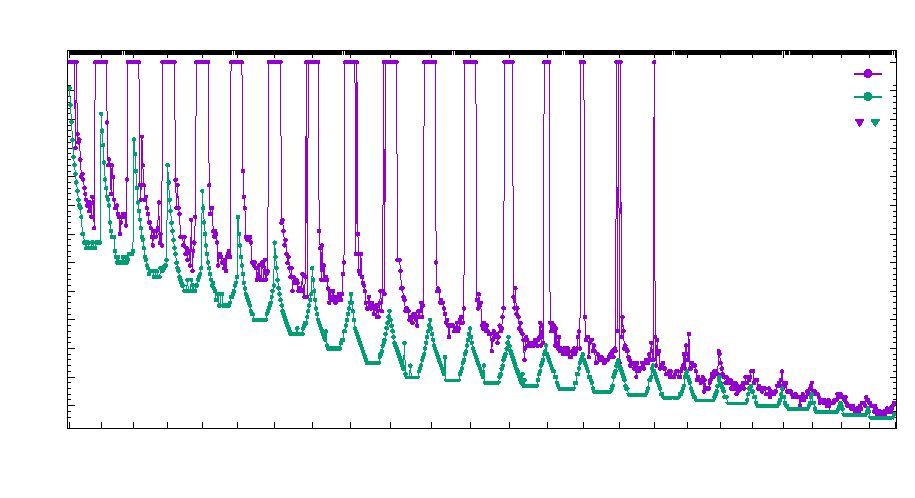
\includegraphics{resultados_7x7}}%
    \gplfronttext
  \end{picture}%
\endgroup
%
	\end{figure}
	}%
\end{frame}

\begin{frame}{Ejemplo ilustrativo en malla de $\mathsf{7\times 7}$}
	\captionsetup[figure]{belowskip = -4pt}%
	\vskip -7pt%
	\begin{figure}[H]
		\caption{Acomodo aleatorio inicial (izquierda) y acomodo encontrado por el algoritmo (derecha), mostrados en diferentes vistas.}%
		\arregloAntesDespues{caso=7x7, separacionAntesDespues=4.2, separacionVertical=0.26cm}{width=4.3cm}[width=4.515cm]{width=2.9cm}%
	\end{figure}
\end{frame}


\begin{frame}{Mallas de $\mathsf{8\times 8}$}
	\vfill
	\Wider[1.85cm]{
	\begin{figure}[H]
		% GNUPLOT: LaTeX picture with Postscript
\begingroup
  % Encoding inside the plot.  In the header of your document, this encoding
  % should to defined, e.g., by using
  % \usepackage[latin1,<other encodings>]{inputenc}
  \inputencoding{latin1}%
  \makeatletter
  \providecommand\color[2][]{%
    \GenericError{(gnuplot) \space\space\space\@spaces}{%
      Package color not loaded in conjunction with
      terminal option `colourtext'%
    }{See the gnuplot documentation for explanation.%
    }{Either use 'blacktext' in gnuplot or load the package
      color.sty in LaTeX.}%
    \renewcommand\color[2][]{}%
  }%
  \providecommand\includegraphics[2][]{%
    \GenericError{(gnuplot) \space\space\space\@spaces}{%
      Package graphicx or graphics not loaded%
    }{See the gnuplot documentation for explanation.%
    }{The gnuplot epslatex terminal needs graphicx.sty or graphics.sty.}%
    \renewcommand\includegraphics[2][]{}%
  }%
  \providecommand\rotatebox[2]{#2}%
  \@ifundefined{ifGPcolor}{%
    \newif\ifGPcolor
    \GPcolortrue
  }{}%
  \@ifundefined{ifGPblacktext}{%
    \newif\ifGPblacktext
    \GPblacktexttrue
  }{}%
  % define a \g@addto@macro without @ in the name:
  \let\gplgaddtomacro\g@addto@macro
  % define empty templates for all commands taking text:
  \gdef\gplbacktext{}%
  \gdef\gplfronttext{}%
  \makeatother
  \ifGPblacktext
    % no textcolor at all
    \def\colorrgb#1{}%
    \def\colorgray#1{}%
  \else
    % gray or color?
    \ifGPcolor
      \def\colorrgb#1{\color[rgb]{#1}}%
      \def\colorgray#1{\color[gray]{#1}}%
      \expandafter\def\csname LTw\endcsname{\color{white}}%
      \expandafter\def\csname LTb\endcsname{\color{black}}%
      \expandafter\def\csname LTa\endcsname{\color{black}}%
      \expandafter\def\csname LT0\endcsname{\color[rgb]{1,0,0}}%
      \expandafter\def\csname LT1\endcsname{\color[rgb]{0,1,0}}%
      \expandafter\def\csname LT2\endcsname{\color[rgb]{0,0,1}}%
      \expandafter\def\csname LT3\endcsname{\color[rgb]{1,0,1}}%
      \expandafter\def\csname LT4\endcsname{\color[rgb]{0,1,1}}%
      \expandafter\def\csname LT5\endcsname{\color[rgb]{1,1,0}}%
      \expandafter\def\csname LT6\endcsname{\color[rgb]{0,0,0}}%
      \expandafter\def\csname LT7\endcsname{\color[rgb]{1,0.3,0}}%
      \expandafter\def\csname LT8\endcsname{\color[rgb]{0.5,0.5,0.5}}%
    \else
      % gray
      \def\colorrgb#1{\color{black}}%
      \def\colorgray#1{\color[gray]{#1}}%
      \expandafter\def\csname LTw\endcsname{\color{white}}%
      \expandafter\def\csname LTb\endcsname{\color{black}}%
      \expandafter\def\csname LTa\endcsname{\color{black}}%
      \expandafter\def\csname LT0\endcsname{\color{black}}%
      \expandafter\def\csname LT1\endcsname{\color{black}}%
      \expandafter\def\csname LT2\endcsname{\color{black}}%
      \expandafter\def\csname LT3\endcsname{\color{black}}%
      \expandafter\def\csname LT4\endcsname{\color{black}}%
      \expandafter\def\csname LT5\endcsname{\color{black}}%
      \expandafter\def\csname LT6\endcsname{\color{black}}%
      \expandafter\def\csname LT7\endcsname{\color{black}}%
      \expandafter\def\csname LT8\endcsname{\color{black}}%
    \fi
  \fi
    \setlength{\unitlength}{0.0500bp}%
    \ifx\gptboxheight\undefined%
      \newlength{\gptboxheight}%
      \newlength{\gptboxwidth}%
      \newsavebox{\gptboxtext}%
    \fi%
    \setlength{\fboxrule}{0.5pt}%
    \setlength{\fboxsep}{1pt}%
\begin{picture}(8466.00,4464.00)%
    \gplgaddtomacro\gplbacktext{%
      \csname LTb\endcsname%%
      \put(448,4048){\makebox(0,0)[r]{\strut{}\raisebox{1pt}{\fontsize{8}{8}\selectfont{$\infty$}}}}%
      \put(448,635){\makebox(0,0)[r]{\strut{}\fontsize{7.8}{7.8}\selectfont{30}}}%
      \put(448,848){\makebox(0,0)[r]{\strut{}\fontsize{7.8}{7.8}\selectfont{40}}}%
      \put(448,1061){\makebox(0,0)[r]{\strut{}\fontsize{7.8}{7.8}\selectfont{50}}}%
      \put(448,1275){\makebox(0,0)[r]{\strut{}\fontsize{7.8}{7.8}\selectfont{60}}}%
      \put(448,1488){\makebox(0,0)[r]{\strut{}\fontsize{7.8}{7.8}\selectfont{70}}}%
      \put(448,1701){\makebox(0,0)[r]{\strut{}\fontsize{7.8}{7.8}\selectfont{80}}}%
      \put(448,1915){\makebox(0,0)[r]{\strut{}\fontsize{7.8}{7.8}\selectfont{90}}}%
      \put(448,2128){\makebox(0,0)[r]{\strut{}\fontsize{7.8}{7.8}\selectfont{100}}}%
      \put(448,2342){\makebox(0,0)[r]{\strut{}\fontsize{7.8}{7.8}\selectfont{110}}}%
      \put(448,2555){\makebox(0,0)[r]{\strut{}\fontsize{7.8}{7.8}\selectfont{120}}}%
      \put(448,2768){\makebox(0,0)[r]{\strut{}\fontsize{7.8}{7.8}\selectfont{130}}}%
      \put(448,2982){\makebox(0,0)[r]{\strut{}\fontsize{7.8}{7.8}\selectfont{140}}}%
      \put(448,3195){\makebox(0,0)[r]{\strut{}\fontsize{7.8}{7.8}\selectfont{150}}}%
      \put(448,3408){\makebox(0,0)[r]{\strut{}\fontsize{7.8}{7.8}\selectfont{160}}}%
      \put(448,3622){\makebox(0,0)[r]{\strut{}\fontsize{7.8}{7.8}\selectfont{170}}}%
      \put(448,3835){\makebox(0,0)[r]{\strut{}\fontsize{7.8}{7.8}\selectfont{180}}}%
      \put(579,462){\rotatebox{45}{\makebox(0,0)[r]{\strut{}\fontsize{6.7}{6.7}\selectfont{48,16}}}}%
      \put(779,462){\rotatebox{45}{\makebox(0,0)[r]{\strut{}\fontsize{6.7}{6.7}\selectfont{48,15}}}}%
      \put(985,462){\rotatebox{45}{\makebox(0,0)[r]{\strut{}\fontsize{6.7}{6.7}\selectfont{48,14}}}}%
      \put(1197,462){\rotatebox{45}{\makebox(0,0)[r]{\strut{}\fontsize{6.7}{6.7}\selectfont{48,13}}}}%
      \put(1415,462){\rotatebox{45}{\makebox(0,0)[r]{\strut{}\fontsize{6.7}{6.7}\selectfont{48,12}}}}%
      \put(1639,462){\rotatebox{45}{\makebox(0,0)[r]{\strut{}\fontsize{6.7}{6.7}\selectfont{48,11}}}}%
      \put(1869,462){\rotatebox{45}{\makebox(0,0)[r]{\strut{}\fontsize{6.7}{6.7}\selectfont{48,10}}}}%
      \put(2105,462){\rotatebox{45}{\makebox(0,0)[r]{\strut{}\fontsize{6.7}{6.7}\selectfont{48,9}}}}%
      \put(2347,462){\rotatebox{45}{\makebox(0,0)[r]{\strut{}\fontsize{6.7}{6.7}\selectfont{48,8}}}}%
      \put(2596,462){\rotatebox{45}{\makebox(0,0)[r]{\strut{}\fontsize{6.7}{6.7}\selectfont{48,7}}}}%
      \put(2850,462){\rotatebox{45}{\makebox(0,0)[r]{\strut{}\fontsize{6.7}{6.7}\selectfont{48,6}}}}%
      \put(3110,462){\rotatebox{45}{\makebox(0,0)[r]{\strut{}\fontsize{6.7}{6.7}\selectfont{48,5}}}}%
      \put(3377,462){\rotatebox{45}{\makebox(0,0)[r]{\strut{}\fontsize{6.7}{6.7}\selectfont{48,4}}}}%
      \put(3649,462){\rotatebox{45}{\makebox(0,0)[r]{\strut{}\fontsize{6.7}{6.7}\selectfont{48,3}}}}%
      \put(3928,462){\rotatebox{45}{\makebox(0,0)[r]{\strut{}\fontsize{6.7}{6.7}\selectfont{48,2}}}}%
      \put(4212,462){\rotatebox{45}{\makebox(0,0)[r]{\strut{}\fontsize{6.7}{6.7}\selectfont{48,1}}}}%
      \put(4503,462){\rotatebox{45}{\makebox(0,0)[r]{\strut{}\fontsize{6.7}{6.7}\selectfont{48,0}}}}%
      \put(4800,462){\rotatebox{45}{\makebox(0,0)[r]{\strut{}\fontsize{6.7}{6.7}\selectfont{47,0}}}}%
      \put(5090,462){\rotatebox{45}{\makebox(0,0)[r]{\strut{}\fontsize{6.7}{6.7}\selectfont{46,0}}}}%
      \put(5375,462){\rotatebox{45}{\makebox(0,0)[r]{\strut{}\fontsize{6.7}{6.7}\selectfont{45,0}}}}%
      \put(5654,462){\rotatebox{45}{\makebox(0,0)[r]{\strut{}\fontsize{6.7}{6.7}\selectfont{44,0}}}}%
      \put(5926,462){\rotatebox{45}{\makebox(0,0)[r]{\strut{}\fontsize{6.7}{6.7}\selectfont{43,0}}}}%
      \put(6193,462){\rotatebox{45}{\makebox(0,0)[r]{\strut{}\fontsize{6.7}{6.7}\selectfont{42,0}}}}%
      \put(6453,462){\rotatebox{45}{\makebox(0,0)[r]{\strut{}\fontsize{6.7}{6.7}\selectfont{41,0}}}}%
      \put(6707,462){\rotatebox{45}{\makebox(0,0)[r]{\strut{}\fontsize{6.7}{6.7}\selectfont{40,0}}}}%
      \put(6956,462){\rotatebox{45}{\makebox(0,0)[r]{\strut{}\fontsize{6.7}{6.7}\selectfont{39,0}}}}%
      \put(7198,462){\rotatebox{45}{\makebox(0,0)[r]{\strut{}\fontsize{6.7}{6.7}\selectfont{38,0}}}}%
      \put(7434,462){\rotatebox{45}{\makebox(0,0)[r]{\strut{}\fontsize{6.7}{6.7}\selectfont{37,0}}}}%
      \put(7664,462){\rotatebox{45}{\makebox(0,0)[r]{\strut{}\fontsize{6.7}{6.7}\selectfont{36,0}}}}%
      \put(7888,462){\rotatebox{45}{\makebox(0,0)[r]{\strut{}\fontsize{6.7}{6.7}\selectfont{35,0}}}}%
      \put(8106,462){\rotatebox{45}{\makebox(0,0)[r]{\strut{}\fontsize{6.7}{6.7}\selectfont{34,0}}}}%
      \put(8318,462){\rotatebox{45}{\makebox(0,0)[r]{\strut{}\fontsize{6.7}{6.7}\selectfont{33,0}}}}%
      \put(8518,462){\rotatebox{45}{\makebox(0,0)[r]{\strut{}\fontsize{6.7}{6.7}\selectfont{0,33}}}}%
      \put(432,4144){\rotatebox{90}{\makebox(0,0)[l]{\strut{}\fontsize{0.2}{0.2}\selectfont{47,17}}}}%
      \put(438,4144){\rotatebox{90}{\makebox(0,0)[l]{\strut{}\fontsize{0.2}{0.2}\selectfont{46,18}}}}%
      \put(444,4144){\rotatebox{90}{\makebox(0,0)[l]{\strut{}\fontsize{0.2}{0.2}\selectfont{45,19}}}}%
      \put(450,4144){\rotatebox{90}{\makebox(0,0)[l]{\strut{}\fontsize{0.2}{0.2}\selectfont{44,20}}}}%
      \put(456,4144){\rotatebox{90}{\makebox(0,0)[l]{\strut{}\fontsize{0.2}{0.2}\selectfont{43,21}}}}%
      \put(462,4144){\rotatebox{90}{\makebox(0,0)[l]{\strut{}\fontsize{0.2}{0.2}\selectfont{42,22}}}}%
      \put(468,4144){\rotatebox{90}{\makebox(0,0)[l]{\strut{}\fontsize{0.2}{0.2}\selectfont{41,23}}}}%
      \put(475,4144){\rotatebox{90}{\makebox(0,0)[l]{\strut{}\fontsize{0.2}{0.2}\selectfont{40,24}}}}%
      \put(481,4144){\rotatebox{90}{\makebox(0,0)[l]{\strut{}\fontsize{0.2}{0.2}\selectfont{39,25}}}}%
      \put(487,4144){\rotatebox{90}{\makebox(0,0)[l]{\strut{}\fontsize{0.2}{0.2}\selectfont{38,26}}}}%
      \put(493,4144){\rotatebox{90}{\makebox(0,0)[l]{\strut{}\fontsize{0.2}{0.2}\selectfont{37,27}}}}%
      \put(499,4144){\rotatebox{90}{\makebox(0,0)[l]{\strut{}\fontsize{0.2}{0.2}\selectfont{36,28}}}}%
      \put(505,4144){\rotatebox{90}{\makebox(0,0)[l]{\strut{}\fontsize{0.2}{0.2}\selectfont{35,29}}}}%
      \put(511,4144){\rotatebox{90}{\makebox(0,0)[l]{\strut{}\fontsize{0.2}{0.2}\selectfont{34,30}}}}%
      \put(517,4144){\rotatebox{90}{\makebox(0,0)[l]{\strut{}\fontsize{0.2}{0.2}\selectfont{33,31}}}}%
      \put(523,4144){\rotatebox{90}{\makebox(0,0)[l]{\strut{}\fontsize{0.2}{0.2}\selectfont{32,32}}}}%
      \put(529,4144){\rotatebox{90}{\makebox(0,0)[l]{\strut{}\fontsize{0.2}{0.2}\selectfont{31,33}}}}%
      \put(535,4144){\rotatebox{90}{\makebox(0,0)[l]{\strut{}\fontsize{0.2}{0.2}\selectfont{30,34}}}}%
      \put(541,4144){\rotatebox{90}{\makebox(0,0)[l]{\strut{}\fontsize{0.2}{0.2}\selectfont{29,35}}}}%
      \put(547,4144){\rotatebox{90}{\makebox(0,0)[l]{\strut{}\fontsize{0.2}{0.2}\selectfont{28,36}}}}%
      \put(553,4144){\rotatebox{90}{\makebox(0,0)[l]{\strut{}\fontsize{0.2}{0.2}\selectfont{27,37}}}}%
      \put(559,4144){\rotatebox{90}{\makebox(0,0)[l]{\strut{}\fontsize{0.2}{0.2}\selectfont{26,38}}}}%
      \put(565,4144){\rotatebox{90}{\makebox(0,0)[l]{\strut{}\fontsize{0.2}{0.2}\selectfont{25,39}}}}%
      \put(571,4144){\rotatebox{90}{\makebox(0,0)[l]{\strut{}\fontsize{0.2}{0.2}\selectfont{24,40}}}}%
      \put(577,4144){\rotatebox{90}{\makebox(0,0)[l]{\strut{}\fontsize{0.2}{0.2}\selectfont{23,41}}}}%
      \put(584,4144){\rotatebox{90}{\makebox(0,0)[l]{\strut{}\fontsize{0.2}{0.2}\selectfont{22,42}}}}%
      \put(590,4144){\rotatebox{90}{\makebox(0,0)[l]{\strut{}\fontsize{0.2}{0.2}\selectfont{21,43}}}}%
      \put(596,4144){\rotatebox{90}{\makebox(0,0)[l]{\strut{}\fontsize{0.2}{0.2}\selectfont{20,44}}}}%
      \put(602,4144){\rotatebox{90}{\makebox(0,0)[l]{\strut{}\fontsize{0.2}{0.2}\selectfont{19,45}}}}%
      \put(608,4144){\rotatebox{90}{\makebox(0,0)[l]{\strut{}\fontsize{0.2}{0.2}\selectfont{18,46}}}}%
      \put(614,4144){\rotatebox{90}{\makebox(0,0)[l]{\strut{}\fontsize{0.2}{0.2}\selectfont{17,47}}}}%
      \put(620,4144){\rotatebox{90}{\makebox(0,0)[l]{\strut{}\fontsize{0.2}{0.2}\selectfont{16,48}}}}%
      \put(632,4144){\rotatebox{90}{\makebox(0,0)[l]{\strut{}\fontsize{0.2}{0.2}\selectfont{47,16}}}}%
      \put(638,4144){\rotatebox{90}{\makebox(0,0)[l]{\strut{}\fontsize{0.2}{0.2}\selectfont{46,17}}}}%
      \put(644,4144){\rotatebox{90}{\makebox(0,0)[l]{\strut{}\fontsize{0.2}{0.2}\selectfont{45,18}}}}%
      \put(650,4144){\rotatebox{90}{\makebox(0,0)[l]{\strut{}\fontsize{0.2}{0.2}\selectfont{44,19}}}}%
      \put(656,4144){\rotatebox{90}{\makebox(0,0)[l]{\strut{}\fontsize{0.2}{0.2}\selectfont{43,20}}}}%
      \put(662,4144){\rotatebox{90}{\makebox(0,0)[l]{\strut{}\fontsize{0.2}{0.2}\selectfont{42,21}}}}%
      \put(668,4144){\rotatebox{90}{\makebox(0,0)[l]{\strut{}\fontsize{0.2}{0.2}\selectfont{41,22}}}}%
      \put(674,4144){\rotatebox{90}{\makebox(0,0)[l]{\strut{}\fontsize{0.2}{0.2}\selectfont{40,23}}}}%
      \put(680,4144){\rotatebox{90}{\makebox(0,0)[l]{\strut{}\fontsize{0.2}{0.2}\selectfont{39,24}}}}%
      \put(686,4144){\rotatebox{90}{\makebox(0,0)[l]{\strut{}\fontsize{0.2}{0.2}\selectfont{38,25}}}}%
      \put(693,4144){\rotatebox{90}{\makebox(0,0)[l]{\strut{}\fontsize{0.2}{0.2}\selectfont{37,26}}}}%
      \put(699,4144){\rotatebox{90}{\makebox(0,0)[l]{\strut{}\fontsize{0.2}{0.2}\selectfont{36,27}}}}%
      \put(705,4144){\rotatebox{90}{\makebox(0,0)[l]{\strut{}\fontsize{0.2}{0.2}\selectfont{35,28}}}}%
      \put(711,4144){\rotatebox{90}{\makebox(0,0)[l]{\strut{}\fontsize{0.2}{0.2}\selectfont{34,29}}}}%
      \put(717,4144){\rotatebox{90}{\makebox(0,0)[l]{\strut{}\fontsize{0.2}{0.2}\selectfont{33,30}}}}%
      \put(723,4144){\rotatebox{90}{\makebox(0,0)[l]{\strut{}\fontsize{0.2}{0.2}\selectfont{32,31}}}}%
      \put(729,4144){\rotatebox{90}{\makebox(0,0)[l]{\strut{}\fontsize{0.2}{0.2}\selectfont{31,32}}}}%
      \put(735,4144){\rotatebox{90}{\makebox(0,0)[l]{\strut{}\fontsize{0.2}{0.2}\selectfont{30,33}}}}%
      \put(741,4144){\rotatebox{90}{\makebox(0,0)[l]{\strut{}\fontsize{0.2}{0.2}\selectfont{29,34}}}}%
      \put(747,4144){\rotatebox{90}{\makebox(0,0)[l]{\strut{}\fontsize{0.2}{0.2}\selectfont{28,35}}}}%
      \put(753,4144){\rotatebox{90}{\makebox(0,0)[l]{\strut{}\fontsize{0.2}{0.2}\selectfont{27,36}}}}%
      \put(759,4144){\rotatebox{90}{\makebox(0,0)[l]{\strut{}\fontsize{0.2}{0.2}\selectfont{26,37}}}}%
      \put(765,4144){\rotatebox{90}{\makebox(0,0)[l]{\strut{}\fontsize{0.2}{0.2}\selectfont{25,38}}}}%
      \put(771,4144){\rotatebox{90}{\makebox(0,0)[l]{\strut{}\fontsize{0.2}{0.2}\selectfont{24,39}}}}%
      \put(777,4144){\rotatebox{90}{\makebox(0,0)[l]{\strut{}\fontsize{0.2}{0.2}\selectfont{23,40}}}}%
      \put(783,4144){\rotatebox{90}{\makebox(0,0)[l]{\strut{}\fontsize{0.2}{0.2}\selectfont{22,41}}}}%
      \put(789,4144){\rotatebox{90}{\makebox(0,0)[l]{\strut{}\fontsize{0.2}{0.2}\selectfont{21,42}}}}%
      \put(795,4144){\rotatebox{90}{\makebox(0,0)[l]{\strut{}\fontsize{0.2}{0.2}\selectfont{20,43}}}}%
      \put(802,4144){\rotatebox{90}{\makebox(0,0)[l]{\strut{}\fontsize{0.2}{0.2}\selectfont{19,44}}}}%
      \put(808,4144){\rotatebox{90}{\makebox(0,0)[l]{\strut{}\fontsize{0.2}{0.2}\selectfont{18,45}}}}%
      \put(814,4144){\rotatebox{90}{\makebox(0,0)[l]{\strut{}\fontsize{0.2}{0.2}\selectfont{17,46}}}}%
      \put(820,4144){\rotatebox{90}{\makebox(0,0)[l]{\strut{}\fontsize{0.2}{0.2}\selectfont{16,47}}}}%
      \put(826,4144){\rotatebox{90}{\makebox(0,0)[l]{\strut{}\fontsize{0.2}{0.2}\selectfont{15,48}}}}%
      \put(838,4144){\rotatebox{90}{\makebox(0,0)[l]{\strut{}\fontsize{0.2}{0.2}\selectfont{47,15}}}}%
      \put(844,4144){\rotatebox{90}{\makebox(0,0)[l]{\strut{}\fontsize{0.2}{0.2}\selectfont{46,16}}}}%
      \put(850,4144){\rotatebox{90}{\makebox(0,0)[l]{\strut{}\fontsize{0.2}{0.2}\selectfont{45,17}}}}%
      \put(856,4144){\rotatebox{90}{\makebox(0,0)[l]{\strut{}\fontsize{0.2}{0.2}\selectfont{44,18}}}}%
      \put(862,4144){\rotatebox{90}{\makebox(0,0)[l]{\strut{}\fontsize{0.2}{0.2}\selectfont{43,19}}}}%
      \put(868,4144){\rotatebox{90}{\makebox(0,0)[l]{\strut{}\fontsize{0.2}{0.2}\selectfont{42,20}}}}%
      \put(874,4144){\rotatebox{90}{\makebox(0,0)[l]{\strut{}\fontsize{0.2}{0.2}\selectfont{41,21}}}}%
      \put(880,4144){\rotatebox{90}{\makebox(0,0)[l]{\strut{}\fontsize{0.2}{0.2}\selectfont{40,22}}}}%
      \put(886,4144){\rotatebox{90}{\makebox(0,0)[l]{\strut{}\fontsize{0.2}{0.2}\selectfont{39,23}}}}%
      \put(892,4144){\rotatebox{90}{\makebox(0,0)[l]{\strut{}\fontsize{0.2}{0.2}\selectfont{38,24}}}}%
      \put(898,4144){\rotatebox{90}{\makebox(0,0)[l]{\strut{}\fontsize{0.2}{0.2}\selectfont{37,25}}}}%
      \put(904,4144){\rotatebox{90}{\makebox(0,0)[l]{\strut{}\fontsize{0.2}{0.2}\selectfont{36,26}}}}%
      \put(911,4144){\rotatebox{90}{\makebox(0,0)[l]{\strut{}\fontsize{0.2}{0.2}\selectfont{35,27}}}}%
      \put(917,4144){\rotatebox{90}{\makebox(0,0)[l]{\strut{}\fontsize{0.2}{0.2}\selectfont{34,28}}}}%
      \put(923,4144){\rotatebox{90}{\makebox(0,0)[l]{\strut{}\fontsize{0.2}{0.2}\selectfont{33,29}}}}%
      \put(929,4144){\rotatebox{90}{\makebox(0,0)[l]{\strut{}\fontsize{0.2}{0.2}\selectfont{32,30}}}}%
      \put(935,4144){\rotatebox{90}{\makebox(0,0)[l]{\strut{}\fontsize{0.2}{0.2}\selectfont{31,31}}}}%
      \put(941,4144){\rotatebox{90}{\makebox(0,0)[l]{\strut{}\fontsize{0.2}{0.2}\selectfont{30,32}}}}%
      \put(947,4144){\rotatebox{90}{\makebox(0,0)[l]{\strut{}\fontsize{0.2}{0.2}\selectfont{29,33}}}}%
      \put(953,4144){\rotatebox{90}{\makebox(0,0)[l]{\strut{}\fontsize{0.2}{0.2}\selectfont{28,34}}}}%
      \put(959,4144){\rotatebox{90}{\makebox(0,0)[l]{\strut{}\fontsize{0.2}{0.2}\selectfont{27,35}}}}%
      \put(965,4144){\rotatebox{90}{\makebox(0,0)[l]{\strut{}\fontsize{0.2}{0.2}\selectfont{26,36}}}}%
      \put(971,4144){\rotatebox{90}{\makebox(0,0)[l]{\strut{}\fontsize{0.2}{0.2}\selectfont{25,37}}}}%
      \put(977,4144){\rotatebox{90}{\makebox(0,0)[l]{\strut{}\fontsize{0.2}{0.2}\selectfont{24,38}}}}%
      \put(983,4144){\rotatebox{90}{\makebox(0,0)[l]{\strut{}\fontsize{0.2}{0.2}\selectfont{23,39}}}}%
      \put(989,4144){\rotatebox{90}{\makebox(0,0)[l]{\strut{}\fontsize{0.2}{0.2}\selectfont{22,40}}}}%
      \put(995,4144){\rotatebox{90}{\makebox(0,0)[l]{\strut{}\fontsize{0.2}{0.2}\selectfont{21,41}}}}%
      \put(1001,4144){\rotatebox{90}{\makebox(0,0)[l]{\strut{}\fontsize{0.2}{0.2}\selectfont{20,42}}}}%
      \put(1007,4144){\rotatebox{90}{\makebox(0,0)[l]{\strut{}\fontsize{0.2}{0.2}\selectfont{19,43}}}}%
      \put(1013,4144){\rotatebox{90}{\makebox(0,0)[l]{\strut{}\fontsize{0.2}{0.2}\selectfont{18,44}}}}%
      \put(1020,4144){\rotatebox{90}{\makebox(0,0)[l]{\strut{}\fontsize{0.2}{0.2}\selectfont{17,45}}}}%
      \put(1026,4144){\rotatebox{90}{\makebox(0,0)[l]{\strut{}\fontsize{0.2}{0.2}\selectfont{16,46}}}}%
      \put(1032,4144){\rotatebox{90}{\makebox(0,0)[l]{\strut{}\fontsize{0.2}{0.2}\selectfont{15,47}}}}%
      \put(1038,4144){\rotatebox{90}{\makebox(0,0)[l]{\strut{}\fontsize{0.2}{0.2}\selectfont{14,48}}}}%
      \put(1050,4144){\rotatebox{90}{\makebox(0,0)[l]{\strut{}\fontsize{0.2}{0.2}\selectfont{47,14}}}}%
      \put(1056,4144){\rotatebox{90}{\makebox(0,0)[l]{\strut{}\fontsize{0.2}{0.2}\selectfont{46,15}}}}%
      \put(1062,4144){\rotatebox{90}{\makebox(0,0)[l]{\strut{}\fontsize{0.2}{0.2}\selectfont{45,16}}}}%
      \put(1068,4144){\rotatebox{90}{\makebox(0,0)[l]{\strut{}\fontsize{0.2}{0.2}\selectfont{44,17}}}}%
      \put(1074,4144){\rotatebox{90}{\makebox(0,0)[l]{\strut{}\fontsize{0.2}{0.2}\selectfont{43,18}}}}%
      \put(1080,4144){\rotatebox{90}{\makebox(0,0)[l]{\strut{}\fontsize{0.2}{0.2}\selectfont{42,19}}}}%
      \put(1086,4144){\rotatebox{90}{\makebox(0,0)[l]{\strut{}\fontsize{0.2}{0.2}\selectfont{41,20}}}}%
      \put(1092,4144){\rotatebox{90}{\makebox(0,0)[l]{\strut{}\fontsize{0.2}{0.2}\selectfont{40,21}}}}%
      \put(1098,4144){\rotatebox{90}{\makebox(0,0)[l]{\strut{}\fontsize{0.2}{0.2}\selectfont{39,22}}}}%
      \put(1104,4144){\rotatebox{90}{\makebox(0,0)[l]{\strut{}\fontsize{0.2}{0.2}\selectfont{38,23}}}}%
      \put(1110,4144){\rotatebox{90}{\makebox(0,0)[l]{\strut{}\fontsize{0.2}{0.2}\selectfont{37,24}}}}%
      \put(1116,4144){\rotatebox{90}{\makebox(0,0)[l]{\strut{}\fontsize{0.2}{0.2}\selectfont{36,25}}}}%
      \put(1122,4144){\rotatebox{90}{\makebox(0,0)[l]{\strut{}\fontsize{0.2}{0.2}\selectfont{35,26}}}}%
      \put(1129,4144){\rotatebox{90}{\makebox(0,0)[l]{\strut{}\fontsize{0.2}{0.2}\selectfont{34,27}}}}%
      \put(1135,4144){\rotatebox{90}{\makebox(0,0)[l]{\strut{}\fontsize{0.2}{0.2}\selectfont{33,28}}}}%
      \put(1141,4144){\rotatebox{90}{\makebox(0,0)[l]{\strut{}\fontsize{0.2}{0.2}\selectfont{32,29}}}}%
      \put(1147,4144){\rotatebox{90}{\makebox(0,0)[l]{\strut{}\fontsize{0.2}{0.2}\selectfont{31,30}}}}%
      \put(1153,4144){\rotatebox{90}{\makebox(0,0)[l]{\strut{}\fontsize{0.2}{0.2}\selectfont{30,31}}}}%
      \put(1159,4144){\rotatebox{90}{\makebox(0,0)[l]{\strut{}\fontsize{0.2}{0.2}\selectfont{29,32}}}}%
      \put(1165,4144){\rotatebox{90}{\makebox(0,0)[l]{\strut{}\fontsize{0.2}{0.2}\selectfont{28,33}}}}%
      \put(1171,4144){\rotatebox{90}{\makebox(0,0)[l]{\strut{}\fontsize{0.2}{0.2}\selectfont{27,34}}}}%
      \put(1177,4144){\rotatebox{90}{\makebox(0,0)[l]{\strut{}\fontsize{0.2}{0.2}\selectfont{26,35}}}}%
      \put(1183,4144){\rotatebox{90}{\makebox(0,0)[l]{\strut{}\fontsize{0.2}{0.2}\selectfont{25,36}}}}%
      \put(1189,4144){\rotatebox{90}{\makebox(0,0)[l]{\strut{}\fontsize{0.2}{0.2}\selectfont{24,37}}}}%
      \put(1195,4144){\rotatebox{90}{\makebox(0,0)[l]{\strut{}\fontsize{0.2}{0.2}\selectfont{23,38}}}}%
      \put(1201,4144){\rotatebox{90}{\makebox(0,0)[l]{\strut{}\fontsize{0.2}{0.2}\selectfont{22,39}}}}%
      \put(1207,4144){\rotatebox{90}{\makebox(0,0)[l]{\strut{}\fontsize{0.2}{0.2}\selectfont{21,40}}}}%
      \put(1213,4144){\rotatebox{90}{\makebox(0,0)[l]{\strut{}\fontsize{0.2}{0.2}\selectfont{20,41}}}}%
      \put(1219,4144){\rotatebox{90}{\makebox(0,0)[l]{\strut{}\fontsize{0.2}{0.2}\selectfont{19,42}}}}%
      \put(1225,4144){\rotatebox{90}{\makebox(0,0)[l]{\strut{}\fontsize{0.2}{0.2}\selectfont{18,43}}}}%
      \put(1231,4144){\rotatebox{90}{\makebox(0,0)[l]{\strut{}\fontsize{0.2}{0.2}\selectfont{17,44}}}}%
      \put(1238,4144){\rotatebox{90}{\makebox(0,0)[l]{\strut{}\fontsize{0.2}{0.2}\selectfont{16,45}}}}%
      \put(1244,4144){\rotatebox{90}{\makebox(0,0)[l]{\strut{}\fontsize{0.2}{0.2}\selectfont{15,46}}}}%
      \put(1250,4144){\rotatebox{90}{\makebox(0,0)[l]{\strut{}\fontsize{0.2}{0.2}\selectfont{14,47}}}}%
      \put(1256,4144){\rotatebox{90}{\makebox(0,0)[l]{\strut{}\fontsize{0.2}{0.2}\selectfont{13,48}}}}%
      \put(1268,4144){\rotatebox{90}{\makebox(0,0)[l]{\strut{}\fontsize{0.2}{0.2}\selectfont{47,13}}}}%
      \put(1274,4144){\rotatebox{90}{\makebox(0,0)[l]{\strut{}\fontsize{0.2}{0.2}\selectfont{46,14}}}}%
      \put(1280,4144){\rotatebox{90}{\makebox(0,0)[l]{\strut{}\fontsize{0.2}{0.2}\selectfont{45,15}}}}%
      \put(1286,4144){\rotatebox{90}{\makebox(0,0)[l]{\strut{}\fontsize{0.2}{0.2}\selectfont{44,16}}}}%
      \put(1292,4144){\rotatebox{90}{\makebox(0,0)[l]{\strut{}\fontsize{0.2}{0.2}\selectfont{43,17}}}}%
      \put(1298,4144){\rotatebox{90}{\makebox(0,0)[l]{\strut{}\fontsize{0.2}{0.2}\selectfont{42,18}}}}%
      \put(1304,4144){\rotatebox{90}{\makebox(0,0)[l]{\strut{}\fontsize{0.2}{0.2}\selectfont{41,19}}}}%
      \put(1310,4144){\rotatebox{90}{\makebox(0,0)[l]{\strut{}\fontsize{0.2}{0.2}\selectfont{40,20}}}}%
      \put(1316,4144){\rotatebox{90}{\makebox(0,0)[l]{\strut{}\fontsize{0.2}{0.2}\selectfont{39,21}}}}%
      \put(1322,4144){\rotatebox{90}{\makebox(0,0)[l]{\strut{}\fontsize{0.2}{0.2}\selectfont{38,22}}}}%
      \put(1328,4144){\rotatebox{90}{\makebox(0,0)[l]{\strut{}\fontsize{0.2}{0.2}\selectfont{37,23}}}}%
      \put(1334,4144){\rotatebox{90}{\makebox(0,0)[l]{\strut{}\fontsize{0.2}{0.2}\selectfont{36,24}}}}%
      \put(1340,4144){\rotatebox{90}{\makebox(0,0)[l]{\strut{}\fontsize{0.2}{0.2}\selectfont{35,25}}}}%
      \put(1347,4144){\rotatebox{90}{\makebox(0,0)[l]{\strut{}\fontsize{0.2}{0.2}\selectfont{34,26}}}}%
      \put(1353,4144){\rotatebox{90}{\makebox(0,0)[l]{\strut{}\fontsize{0.2}{0.2}\selectfont{33,27}}}}%
      \put(1359,4144){\rotatebox{90}{\makebox(0,0)[l]{\strut{}\fontsize{0.2}{0.2}\selectfont{32,28}}}}%
      \put(1365,4144){\rotatebox{90}{\makebox(0,0)[l]{\strut{}\fontsize{0.2}{0.2}\selectfont{31,29}}}}%
      \put(1371,4144){\rotatebox{90}{\makebox(0,0)[l]{\strut{}\fontsize{0.2}{0.2}\selectfont{30,30}}}}%
      \put(1377,4144){\rotatebox{90}{\makebox(0,0)[l]{\strut{}\fontsize{0.2}{0.2}\selectfont{29,31}}}}%
      \put(1383,4144){\rotatebox{90}{\makebox(0,0)[l]{\strut{}\fontsize{0.2}{0.2}\selectfont{28,32}}}}%
      \put(1389,4144){\rotatebox{90}{\makebox(0,0)[l]{\strut{}\fontsize{0.2}{0.2}\selectfont{27,33}}}}%
      \put(1395,4144){\rotatebox{90}{\makebox(0,0)[l]{\strut{}\fontsize{0.2}{0.2}\selectfont{26,34}}}}%
      \put(1401,4144){\rotatebox{90}{\makebox(0,0)[l]{\strut{}\fontsize{0.2}{0.2}\selectfont{25,35}}}}%
      \put(1407,4144){\rotatebox{90}{\makebox(0,0)[l]{\strut{}\fontsize{0.2}{0.2}\selectfont{24,36}}}}%
      \put(1413,4144){\rotatebox{90}{\makebox(0,0)[l]{\strut{}\fontsize{0.2}{0.2}\selectfont{23,37}}}}%
      \put(1419,4144){\rotatebox{90}{\makebox(0,0)[l]{\strut{}\fontsize{0.2}{0.2}\selectfont{22,38}}}}%
      \put(1425,4144){\rotatebox{90}{\makebox(0,0)[l]{\strut{}\fontsize{0.2}{0.2}\selectfont{21,39}}}}%
      \put(1431,4144){\rotatebox{90}{\makebox(0,0)[l]{\strut{}\fontsize{0.2}{0.2}\selectfont{20,40}}}}%
      \put(1437,4144){\rotatebox{90}{\makebox(0,0)[l]{\strut{}\fontsize{0.2}{0.2}\selectfont{19,41}}}}%
      \put(1443,4144){\rotatebox{90}{\makebox(0,0)[l]{\strut{}\fontsize{0.2}{0.2}\selectfont{18,42}}}}%
      \put(1449,4144){\rotatebox{90}{\makebox(0,0)[l]{\strut{}\fontsize{0.2}{0.2}\selectfont{17,43}}}}%
      \put(1456,4144){\rotatebox{90}{\makebox(0,0)[l]{\strut{}\fontsize{0.2}{0.2}\selectfont{16,44}}}}%
      \put(1462,4144){\rotatebox{90}{\makebox(0,0)[l]{\strut{}\fontsize{0.2}{0.2}\selectfont{15,45}}}}%
      \put(1468,4144){\rotatebox{90}{\makebox(0,0)[l]{\strut{}\fontsize{0.2}{0.2}\selectfont{14,46}}}}%
      \put(1474,4144){\rotatebox{90}{\makebox(0,0)[l]{\strut{}\fontsize{0.2}{0.2}\selectfont{13,47}}}}%
      \put(1480,4144){\rotatebox{90}{\makebox(0,0)[l]{\strut{}\fontsize{0.2}{0.2}\selectfont{12,48}}}}%
      \put(1492,4144){\rotatebox{90}{\makebox(0,0)[l]{\strut{}\fontsize{0.2}{0.2}\selectfont{47,12}}}}%
      \put(1498,4144){\rotatebox{90}{\makebox(0,0)[l]{\strut{}\fontsize{0.2}{0.2}\selectfont{46,13}}}}%
      \put(1504,4144){\rotatebox{90}{\makebox(0,0)[l]{\strut{}\fontsize{0.2}{0.2}\selectfont{45,14}}}}%
      \put(1510,4144){\rotatebox{90}{\makebox(0,0)[l]{\strut{}\fontsize{0.2}{0.2}\selectfont{44,15}}}}%
      \put(1516,4144){\rotatebox{90}{\makebox(0,0)[l]{\strut{}\fontsize{0.2}{0.2}\selectfont{43,16}}}}%
      \put(1522,4144){\rotatebox{90}{\makebox(0,0)[l]{\strut{}\fontsize{0.2}{0.2}\selectfont{42,17}}}}%
      \put(1528,4144){\rotatebox{90}{\makebox(0,0)[l]{\strut{}\fontsize{0.2}{0.2}\selectfont{41,18}}}}%
      \put(1534,4144){\rotatebox{90}{\makebox(0,0)[l]{\strut{}\fontsize{0.2}{0.2}\selectfont{40,19}}}}%
      \put(1540,4144){\rotatebox{90}{\makebox(0,0)[l]{\strut{}\fontsize{0.2}{0.2}\selectfont{39,20}}}}%
      \put(1546,4144){\rotatebox{90}{\makebox(0,0)[l]{\strut{}\fontsize{0.2}{0.2}\selectfont{38,21}}}}%
      \put(1552,4144){\rotatebox{90}{\makebox(0,0)[l]{\strut{}\fontsize{0.2}{0.2}\selectfont{37,22}}}}%
      \put(1558,4144){\rotatebox{90}{\makebox(0,0)[l]{\strut{}\fontsize{0.2}{0.2}\selectfont{36,23}}}}%
      \put(1565,4144){\rotatebox{90}{\makebox(0,0)[l]{\strut{}\fontsize{0.2}{0.2}\selectfont{35,24}}}}%
      \put(1571,4144){\rotatebox{90}{\makebox(0,0)[l]{\strut{}\fontsize{0.2}{0.2}\selectfont{34,25}}}}%
      \put(1577,4144){\rotatebox{90}{\makebox(0,0)[l]{\strut{}\fontsize{0.2}{0.2}\selectfont{33,26}}}}%
      \put(1583,4144){\rotatebox{90}{\makebox(0,0)[l]{\strut{}\fontsize{0.2}{0.2}\selectfont{32,27}}}}%
      \put(1589,4144){\rotatebox{90}{\makebox(0,0)[l]{\strut{}\fontsize{0.2}{0.2}\selectfont{31,28}}}}%
      \put(1595,4144){\rotatebox{90}{\makebox(0,0)[l]{\strut{}\fontsize{0.2}{0.2}\selectfont{30,29}}}}%
      \put(1601,4144){\rotatebox{90}{\makebox(0,0)[l]{\strut{}\fontsize{0.2}{0.2}\selectfont{29,30}}}}%
      \put(1607,4144){\rotatebox{90}{\makebox(0,0)[l]{\strut{}\fontsize{0.2}{0.2}\selectfont{28,31}}}}%
      \put(1613,4144){\rotatebox{90}{\makebox(0,0)[l]{\strut{}\fontsize{0.2}{0.2}\selectfont{27,32}}}}%
      \put(1619,4144){\rotatebox{90}{\makebox(0,0)[l]{\strut{}\fontsize{0.2}{0.2}\selectfont{26,33}}}}%
      \put(1625,4144){\rotatebox{90}{\makebox(0,0)[l]{\strut{}\fontsize{0.2}{0.2}\selectfont{25,34}}}}%
      \put(1631,4144){\rotatebox{90}{\makebox(0,0)[l]{\strut{}\fontsize{0.2}{0.2}\selectfont{24,35}}}}%
      \put(1637,4144){\rotatebox{90}{\makebox(0,0)[l]{\strut{}\fontsize{0.2}{0.2}\selectfont{23,36}}}}%
      \put(1643,4144){\rotatebox{90}{\makebox(0,0)[l]{\strut{}\fontsize{0.2}{0.2}\selectfont{22,37}}}}%
      \put(1649,4144){\rotatebox{90}{\makebox(0,0)[l]{\strut{}\fontsize{0.2}{0.2}\selectfont{21,38}}}}%
      \put(1655,4144){\rotatebox{90}{\makebox(0,0)[l]{\strut{}\fontsize{0.2}{0.2}\selectfont{20,39}}}}%
      \put(1661,4144){\rotatebox{90}{\makebox(0,0)[l]{\strut{}\fontsize{0.2}{0.2}\selectfont{19,40}}}}%
      \put(1667,4144){\rotatebox{90}{\makebox(0,0)[l]{\strut{}\fontsize{0.2}{0.2}\selectfont{18,41}}}}%
      \put(1674,4144){\rotatebox{90}{\makebox(0,0)[l]{\strut{}\fontsize{0.2}{0.2}\selectfont{17,42}}}}%
      \put(1680,4144){\rotatebox{90}{\makebox(0,0)[l]{\strut{}\fontsize{0.2}{0.2}\selectfont{16,43}}}}%
      \put(1686,4144){\rotatebox{90}{\makebox(0,0)[l]{\strut{}\fontsize{0.2}{0.2}\selectfont{15,44}}}}%
      \put(1692,4144){\rotatebox{90}{\makebox(0,0)[l]{\strut{}\fontsize{0.2}{0.2}\selectfont{14,45}}}}%
      \put(1698,4144){\rotatebox{90}{\makebox(0,0)[l]{\strut{}\fontsize{0.2}{0.2}\selectfont{13,46}}}}%
      \put(1704,4144){\rotatebox{90}{\makebox(0,0)[l]{\strut{}\fontsize{0.2}{0.2}\selectfont{12,47}}}}%
      \put(1710,4144){\rotatebox{90}{\makebox(0,0)[l]{\strut{}\fontsize{0.2}{0.2}\selectfont{11,48}}}}%
      \put(1722,4144){\rotatebox{90}{\makebox(0,0)[l]{\strut{}\fontsize{0.2}{0.2}\selectfont{47,11}}}}%
      \put(1728,4144){\rotatebox{90}{\makebox(0,0)[l]{\strut{}\fontsize{0.2}{0.2}\selectfont{46,12}}}}%
      \put(1734,4144){\rotatebox{90}{\makebox(0,0)[l]{\strut{}\fontsize{0.2}{0.2}\selectfont{45,13}}}}%
      \put(1740,4144){\rotatebox{90}{\makebox(0,0)[l]{\strut{}\fontsize{0.2}{0.2}\selectfont{44,14}}}}%
      \put(1746,4144){\rotatebox{90}{\makebox(0,0)[l]{\strut{}\fontsize{0.2}{0.2}\selectfont{43,15}}}}%
      \put(1752,4144){\rotatebox{90}{\makebox(0,0)[l]{\strut{}\fontsize{0.2}{0.2}\selectfont{42,16}}}}%
      \put(1758,4144){\rotatebox{90}{\makebox(0,0)[l]{\strut{}\fontsize{0.2}{0.2}\selectfont{41,17}}}}%
      \put(1764,4144){\rotatebox{90}{\makebox(0,0)[l]{\strut{}\fontsize{0.2}{0.2}\selectfont{40,18}}}}%
      \put(1770,4144){\rotatebox{90}{\makebox(0,0)[l]{\strut{}\fontsize{0.2}{0.2}\selectfont{39,19}}}}%
      \put(1776,4144){\rotatebox{90}{\makebox(0,0)[l]{\strut{}\fontsize{0.2}{0.2}\selectfont{38,20}}}}%
      \put(1783,4144){\rotatebox{90}{\makebox(0,0)[l]{\strut{}\fontsize{0.2}{0.2}\selectfont{37,21}}}}%
      \put(1789,4144){\rotatebox{90}{\makebox(0,0)[l]{\strut{}\fontsize{0.2}{0.2}\selectfont{36,22}}}}%
      \put(1795,4144){\rotatebox{90}{\makebox(0,0)[l]{\strut{}\fontsize{0.2}{0.2}\selectfont{35,23}}}}%
      \put(1801,4144){\rotatebox{90}{\makebox(0,0)[l]{\strut{}\fontsize{0.2}{0.2}\selectfont{34,24}}}}%
      \put(1807,4144){\rotatebox{90}{\makebox(0,0)[l]{\strut{}\fontsize{0.2}{0.2}\selectfont{33,25}}}}%
      \put(1813,4144){\rotatebox{90}{\makebox(0,0)[l]{\strut{}\fontsize{0.2}{0.2}\selectfont{32,26}}}}%
      \put(1819,4144){\rotatebox{90}{\makebox(0,0)[l]{\strut{}\fontsize{0.2}{0.2}\selectfont{31,27}}}}%
      \put(1825,4144){\rotatebox{90}{\makebox(0,0)[l]{\strut{}\fontsize{0.2}{0.2}\selectfont{30,28}}}}%
      \put(1831,4144){\rotatebox{90}{\makebox(0,0)[l]{\strut{}\fontsize{0.2}{0.2}\selectfont{29,29}}}}%
      \put(1837,4144){\rotatebox{90}{\makebox(0,0)[l]{\strut{}\fontsize{0.2}{0.2}\selectfont{28,30}}}}%
      \put(1843,4144){\rotatebox{90}{\makebox(0,0)[l]{\strut{}\fontsize{0.2}{0.2}\selectfont{27,31}}}}%
      \put(1849,4144){\rotatebox{90}{\makebox(0,0)[l]{\strut{}\fontsize{0.2}{0.2}\selectfont{26,32}}}}%
      \put(1855,4144){\rotatebox{90}{\makebox(0,0)[l]{\strut{}\fontsize{0.2}{0.2}\selectfont{25,33}}}}%
      \put(1861,4144){\rotatebox{90}{\makebox(0,0)[l]{\strut{}\fontsize{0.2}{0.2}\selectfont{24,34}}}}%
      \put(1867,4144){\rotatebox{90}{\makebox(0,0)[l]{\strut{}\fontsize{0.2}{0.2}\selectfont{23,35}}}}%
      \put(1873,4144){\rotatebox{90}{\makebox(0,0)[l]{\strut{}\fontsize{0.2}{0.2}\selectfont{22,36}}}}%
      \put(1879,4144){\rotatebox{90}{\makebox(0,0)[l]{\strut{}\fontsize{0.2}{0.2}\selectfont{21,37}}}}%
      \put(1885,4144){\rotatebox{90}{\makebox(0,0)[l]{\strut{}\fontsize{0.2}{0.2}\selectfont{20,38}}}}%
      \put(1892,4144){\rotatebox{90}{\makebox(0,0)[l]{\strut{}\fontsize{0.2}{0.2}\selectfont{19,39}}}}%
      \put(1898,4144){\rotatebox{90}{\makebox(0,0)[l]{\strut{}\fontsize{0.2}{0.2}\selectfont{18,40}}}}%
      \put(1904,4144){\rotatebox{90}{\makebox(0,0)[l]{\strut{}\fontsize{0.2}{0.2}\selectfont{17,41}}}}%
      \put(1910,4144){\rotatebox{90}{\makebox(0,0)[l]{\strut{}\fontsize{0.2}{0.2}\selectfont{16,42}}}}%
      \put(1916,4144){\rotatebox{90}{\makebox(0,0)[l]{\strut{}\fontsize{0.2}{0.2}\selectfont{15,43}}}}%
      \put(1922,4144){\rotatebox{90}{\makebox(0,0)[l]{\strut{}\fontsize{0.2}{0.2}\selectfont{14,44}}}}%
      \put(1928,4144){\rotatebox{90}{\makebox(0,0)[l]{\strut{}\fontsize{0.2}{0.2}\selectfont{13,45}}}}%
      \put(1934,4144){\rotatebox{90}{\makebox(0,0)[l]{\strut{}\fontsize{0.2}{0.2}\selectfont{12,46}}}}%
      \put(1940,4144){\rotatebox{90}{\makebox(0,0)[l]{\strut{}\fontsize{0.2}{0.2}\selectfont{11,47}}}}%
      \put(1946,4144){\rotatebox{90}{\makebox(0,0)[l]{\strut{}\fontsize{0.2}{0.2}\selectfont{10,48}}}}%
      \put(1958,4144){\rotatebox{90}{\makebox(0,0)[l]{\strut{}\fontsize{0.2}{0.2}\selectfont{47,10}}}}%
      \put(1964,4144){\rotatebox{90}{\makebox(0,0)[l]{\strut{}\fontsize{0.2}{0.2}\selectfont{46,11}}}}%
      \put(1970,4144){\rotatebox{90}{\makebox(0,0)[l]{\strut{}\fontsize{0.2}{0.2}\selectfont{45,12}}}}%
      \put(1976,4144){\rotatebox{90}{\makebox(0,0)[l]{\strut{}\fontsize{0.2}{0.2}\selectfont{44,13}}}}%
      \put(1982,4144){\rotatebox{90}{\makebox(0,0)[l]{\strut{}\fontsize{0.2}{0.2}\selectfont{43,14}}}}%
      \put(1988,4144){\rotatebox{90}{\makebox(0,0)[l]{\strut{}\fontsize{0.2}{0.2}\selectfont{42,15}}}}%
      \put(1994,4144){\rotatebox{90}{\makebox(0,0)[l]{\strut{}\fontsize{0.2}{0.2}\selectfont{41,16}}}}%
      \put(2001,4144){\rotatebox{90}{\makebox(0,0)[l]{\strut{}\fontsize{0.2}{0.2}\selectfont{40,17}}}}%
      \put(2007,4144){\rotatebox{90}{\makebox(0,0)[l]{\strut{}\fontsize{0.2}{0.2}\selectfont{39,18}}}}%
      \put(2013,4144){\rotatebox{90}{\makebox(0,0)[l]{\strut{}\fontsize{0.2}{0.2}\selectfont{38,19}}}}%
      \put(2019,4144){\rotatebox{90}{\makebox(0,0)[l]{\strut{}\fontsize{0.2}{0.2}\selectfont{37,20}}}}%
      \put(2025,4144){\rotatebox{90}{\makebox(0,0)[l]{\strut{}\fontsize{0.2}{0.2}\selectfont{36,21}}}}%
      \put(2031,4144){\rotatebox{90}{\makebox(0,0)[l]{\strut{}\fontsize{0.2}{0.2}\selectfont{35,22}}}}%
      \put(2037,4144){\rotatebox{90}{\makebox(0,0)[l]{\strut{}\fontsize{0.2}{0.2}\selectfont{34,23}}}}%
      \put(2043,4144){\rotatebox{90}{\makebox(0,0)[l]{\strut{}\fontsize{0.2}{0.2}\selectfont{33,24}}}}%
      \put(2049,4144){\rotatebox{90}{\makebox(0,0)[l]{\strut{}\fontsize{0.2}{0.2}\selectfont{32,25}}}}%
      \put(2055,4144){\rotatebox{90}{\makebox(0,0)[l]{\strut{}\fontsize{0.2}{0.2}\selectfont{31,26}}}}%
      \put(2061,4144){\rotatebox{90}{\makebox(0,0)[l]{\strut{}\fontsize{0.2}{0.2}\selectfont{30,27}}}}%
      \put(2067,4144){\rotatebox{90}{\makebox(0,0)[l]{\strut{}\fontsize{0.2}{0.2}\selectfont{29,28}}}}%
      \put(2073,4144){\rotatebox{90}{\makebox(0,0)[l]{\strut{}\fontsize{0.2}{0.2}\selectfont{28,29}}}}%
      \put(2079,4144){\rotatebox{90}{\makebox(0,0)[l]{\strut{}\fontsize{0.2}{0.2}\selectfont{27,30}}}}%
      \put(2085,4144){\rotatebox{90}{\makebox(0,0)[l]{\strut{}\fontsize{0.2}{0.2}\selectfont{26,31}}}}%
      \put(2091,4144){\rotatebox{90}{\makebox(0,0)[l]{\strut{}\fontsize{0.2}{0.2}\selectfont{25,32}}}}%
      \put(2097,4144){\rotatebox{90}{\makebox(0,0)[l]{\strut{}\fontsize{0.2}{0.2}\selectfont{24,33}}}}%
      \put(2103,4144){\rotatebox{90}{\makebox(0,0)[l]{\strut{}\fontsize{0.2}{0.2}\selectfont{23,34}}}}%
      \put(2110,4144){\rotatebox{90}{\makebox(0,0)[l]{\strut{}\fontsize{0.2}{0.2}\selectfont{22,35}}}}%
      \put(2116,4144){\rotatebox{90}{\makebox(0,0)[l]{\strut{}\fontsize{0.2}{0.2}\selectfont{21,36}}}}%
      \put(2122,4144){\rotatebox{90}{\makebox(0,0)[l]{\strut{}\fontsize{0.2}{0.2}\selectfont{20,37}}}}%
      \put(2128,4144){\rotatebox{90}{\makebox(0,0)[l]{\strut{}\fontsize{0.2}{0.2}\selectfont{19,38}}}}%
      \put(2134,4144){\rotatebox{90}{\makebox(0,0)[l]{\strut{}\fontsize{0.2}{0.2}\selectfont{18,39}}}}%
      \put(2140,4144){\rotatebox{90}{\makebox(0,0)[l]{\strut{}\fontsize{0.2}{0.2}\selectfont{17,40}}}}%
      \put(2146,4144){\rotatebox{90}{\makebox(0,0)[l]{\strut{}\fontsize{0.2}{0.2}\selectfont{16,41}}}}%
      \put(2152,4144){\rotatebox{90}{\makebox(0,0)[l]{\strut{}\fontsize{0.2}{0.2}\selectfont{15,42}}}}%
      \put(2158,4144){\rotatebox{90}{\makebox(0,0)[l]{\strut{}\fontsize{0.2}{0.2}\selectfont{14,43}}}}%
      \put(2164,4144){\rotatebox{90}{\makebox(0,0)[l]{\strut{}\fontsize{0.2}{0.2}\selectfont{13,44}}}}%
      \put(2170,4144){\rotatebox{90}{\makebox(0,0)[l]{\strut{}\fontsize{0.2}{0.2}\selectfont{12,45}}}}%
      \put(2176,4144){\rotatebox{90}{\makebox(0,0)[l]{\strut{}\fontsize{0.2}{0.2}\selectfont{11,46}}}}%
      \put(2182,4144){\rotatebox{90}{\makebox(0,0)[l]{\strut{}\fontsize{0.2}{0.2}\selectfont{10,47}}}}%
      \put(2188,4144){\rotatebox{90}{\makebox(0,0)[l]{\strut{}\fontsize{0.2}{0.2}\selectfont{9,48}}}}%
      \put(2200,4144){\rotatebox{90}{\makebox(0,0)[l]{\strut{}\fontsize{0.2}{0.2}\selectfont{47,9}}}}%
      \put(2206,4144){\rotatebox{90}{\makebox(0,0)[l]{\strut{}\fontsize{0.2}{0.2}\selectfont{46,10}}}}%
      \put(2212,4144){\rotatebox{90}{\makebox(0,0)[l]{\strut{}\fontsize{0.2}{0.2}\selectfont{45,11}}}}%
      \put(2219,4144){\rotatebox{90}{\makebox(0,0)[l]{\strut{}\fontsize{0.2}{0.2}\selectfont{44,12}}}}%
      \put(2225,4144){\rotatebox{90}{\makebox(0,0)[l]{\strut{}\fontsize{0.2}{0.2}\selectfont{43,13}}}}%
      \put(2231,4144){\rotatebox{90}{\makebox(0,0)[l]{\strut{}\fontsize{0.2}{0.2}\selectfont{42,14}}}}%
      \put(2237,4144){\rotatebox{90}{\makebox(0,0)[l]{\strut{}\fontsize{0.2}{0.2}\selectfont{41,15}}}}%
      \put(2243,4144){\rotatebox{90}{\makebox(0,0)[l]{\strut{}\fontsize{0.2}{0.2}\selectfont{40,16}}}}%
      \put(2249,4144){\rotatebox{90}{\makebox(0,0)[l]{\strut{}\fontsize{0.2}{0.2}\selectfont{39,17}}}}%
      \put(2255,4144){\rotatebox{90}{\makebox(0,0)[l]{\strut{}\fontsize{0.2}{0.2}\selectfont{38,18}}}}%
      \put(2261,4144){\rotatebox{90}{\makebox(0,0)[l]{\strut{}\fontsize{0.2}{0.2}\selectfont{37,19}}}}%
      \put(2267,4144){\rotatebox{90}{\makebox(0,0)[l]{\strut{}\fontsize{0.2}{0.2}\selectfont{36,20}}}}%
      \put(2273,4144){\rotatebox{90}{\makebox(0,0)[l]{\strut{}\fontsize{0.2}{0.2}\selectfont{35,21}}}}%
      \put(2279,4144){\rotatebox{90}{\makebox(0,0)[l]{\strut{}\fontsize{0.2}{0.2}\selectfont{34,22}}}}%
      \put(2285,4144){\rotatebox{90}{\makebox(0,0)[l]{\strut{}\fontsize{0.2}{0.2}\selectfont{33,23}}}}%
      \put(2291,4144){\rotatebox{90}{\makebox(0,0)[l]{\strut{}\fontsize{0.2}{0.2}\selectfont{32,24}}}}%
      \put(2297,4144){\rotatebox{90}{\makebox(0,0)[l]{\strut{}\fontsize{0.2}{0.2}\selectfont{31,25}}}}%
      \put(2303,4144){\rotatebox{90}{\makebox(0,0)[l]{\strut{}\fontsize{0.2}{0.2}\selectfont{30,26}}}}%
      \put(2309,4144){\rotatebox{90}{\makebox(0,0)[l]{\strut{}\fontsize{0.2}{0.2}\selectfont{29,27}}}}%
      \put(2315,4144){\rotatebox{90}{\makebox(0,0)[l]{\strut{}\fontsize{0.2}{0.2}\selectfont{28,28}}}}%
      \put(2321,4144){\rotatebox{90}{\makebox(0,0)[l]{\strut{}\fontsize{0.2}{0.2}\selectfont{27,29}}}}%
      \put(2328,4144){\rotatebox{90}{\makebox(0,0)[l]{\strut{}\fontsize{0.2}{0.2}\selectfont{26,30}}}}%
      \put(2334,4144){\rotatebox{90}{\makebox(0,0)[l]{\strut{}\fontsize{0.2}{0.2}\selectfont{25,31}}}}%
      \put(2340,4144){\rotatebox{90}{\makebox(0,0)[l]{\strut{}\fontsize{0.2}{0.2}\selectfont{24,32}}}}%
      \put(2346,4144){\rotatebox{90}{\makebox(0,0)[l]{\strut{}\fontsize{0.2}{0.2}\selectfont{23,33}}}}%
      \put(2352,4144){\rotatebox{90}{\makebox(0,0)[l]{\strut{}\fontsize{0.2}{0.2}\selectfont{22,34}}}}%
      \put(2358,4144){\rotatebox{90}{\makebox(0,0)[l]{\strut{}\fontsize{0.2}{0.2}\selectfont{21,35}}}}%
      \put(2364,4144){\rotatebox{90}{\makebox(0,0)[l]{\strut{}\fontsize{0.2}{0.2}\selectfont{20,36}}}}%
      \put(2370,4144){\rotatebox{90}{\makebox(0,0)[l]{\strut{}\fontsize{0.2}{0.2}\selectfont{19,37}}}}%
      \put(2376,4144){\rotatebox{90}{\makebox(0,0)[l]{\strut{}\fontsize{0.2}{0.2}\selectfont{18,38}}}}%
      \put(2382,4144){\rotatebox{90}{\makebox(0,0)[l]{\strut{}\fontsize{0.2}{0.2}\selectfont{17,39}}}}%
      \put(2388,4144){\rotatebox{90}{\makebox(0,0)[l]{\strut{}\fontsize{0.2}{0.2}\selectfont{16,40}}}}%
      \put(2394,4144){\rotatebox{90}{\makebox(0,0)[l]{\strut{}\fontsize{0.2}{0.2}\selectfont{15,41}}}}%
      \put(2400,4144){\rotatebox{90}{\makebox(0,0)[l]{\strut{}\fontsize{0.2}{0.2}\selectfont{14,42}}}}%
      \put(2406,4144){\rotatebox{90}{\makebox(0,0)[l]{\strut{}\fontsize{0.2}{0.2}\selectfont{13,43}}}}%
      \put(2412,4144){\rotatebox{90}{\makebox(0,0)[l]{\strut{}\fontsize{0.2}{0.2}\selectfont{12,44}}}}%
      \put(2418,4144){\rotatebox{90}{\makebox(0,0)[l]{\strut{}\fontsize{0.2}{0.2}\selectfont{11,45}}}}%
      \put(2424,4144){\rotatebox{90}{\makebox(0,0)[l]{\strut{}\fontsize{0.2}{0.2}\selectfont{10,46}}}}%
      \put(2430,4144){\rotatebox{90}{\makebox(0,0)[l]{\strut{}\fontsize{0.2}{0.2}\selectfont{9,47}}}}%
      \put(2437,4144){\rotatebox{90}{\makebox(0,0)[l]{\strut{}\fontsize{0.2}{0.2}\selectfont{8,48}}}}%
      \put(2449,4144){\rotatebox{90}{\makebox(0,0)[l]{\strut{}\fontsize{0.2}{0.2}\selectfont{47,8}}}}%
      \put(2455,4144){\rotatebox{90}{\makebox(0,0)[l]{\strut{}\fontsize{0.2}{0.2}\selectfont{46,9}}}}%
      \put(2461,4144){\rotatebox{90}{\makebox(0,0)[l]{\strut{}\fontsize{0.2}{0.2}\selectfont{45,10}}}}%
      \put(2467,4144){\rotatebox{90}{\makebox(0,0)[l]{\strut{}\fontsize{0.2}{0.2}\selectfont{44,11}}}}%
      \put(2473,4144){\rotatebox{90}{\makebox(0,0)[l]{\strut{}\fontsize{0.2}{0.2}\selectfont{43,12}}}}%
      \put(2479,4144){\rotatebox{90}{\makebox(0,0)[l]{\strut{}\fontsize{0.2}{0.2}\selectfont{42,13}}}}%
      \put(2485,4144){\rotatebox{90}{\makebox(0,0)[l]{\strut{}\fontsize{0.2}{0.2}\selectfont{41,14}}}}%
      \put(2491,4144){\rotatebox{90}{\makebox(0,0)[l]{\strut{}\fontsize{0.2}{0.2}\selectfont{40,15}}}}%
      \put(2497,4144){\rotatebox{90}{\makebox(0,0)[l]{\strut{}\fontsize{0.2}{0.2}\selectfont{39,16}}}}%
      \put(2503,4144){\rotatebox{90}{\makebox(0,0)[l]{\strut{}\fontsize{0.2}{0.2}\selectfont{38,17}}}}%
      \put(2509,4144){\rotatebox{90}{\makebox(0,0)[l]{\strut{}\fontsize{0.2}{0.2}\selectfont{37,18}}}}%
      \put(2515,4144){\rotatebox{90}{\makebox(0,0)[l]{\strut{}\fontsize{0.2}{0.2}\selectfont{36,19}}}}%
      \put(2521,4144){\rotatebox{90}{\makebox(0,0)[l]{\strut{}\fontsize{0.2}{0.2}\selectfont{35,20}}}}%
      \put(2527,4144){\rotatebox{90}{\makebox(0,0)[l]{\strut{}\fontsize{0.2}{0.2}\selectfont{34,21}}}}%
      \put(2533,4144){\rotatebox{90}{\makebox(0,0)[l]{\strut{}\fontsize{0.2}{0.2}\selectfont{33,22}}}}%
      \put(2539,4144){\rotatebox{90}{\makebox(0,0)[l]{\strut{}\fontsize{0.2}{0.2}\selectfont{32,23}}}}%
      \put(2546,4144){\rotatebox{90}{\makebox(0,0)[l]{\strut{}\fontsize{0.2}{0.2}\selectfont{31,24}}}}%
      \put(2552,4144){\rotatebox{90}{\makebox(0,0)[l]{\strut{}\fontsize{0.2}{0.2}\selectfont{30,25}}}}%
      \put(2558,4144){\rotatebox{90}{\makebox(0,0)[l]{\strut{}\fontsize{0.2}{0.2}\selectfont{29,26}}}}%
      \put(2564,4144){\rotatebox{90}{\makebox(0,0)[l]{\strut{}\fontsize{0.2}{0.2}\selectfont{28,27}}}}%
      \put(2570,4144){\rotatebox{90}{\makebox(0,0)[l]{\strut{}\fontsize{0.2}{0.2}\selectfont{27,28}}}}%
      \put(2576,4144){\rotatebox{90}{\makebox(0,0)[l]{\strut{}\fontsize{0.2}{0.2}\selectfont{26,29}}}}%
      \put(2582,4144){\rotatebox{90}{\makebox(0,0)[l]{\strut{}\fontsize{0.2}{0.2}\selectfont{25,30}}}}%
      \put(2588,4144){\rotatebox{90}{\makebox(0,0)[l]{\strut{}\fontsize{0.2}{0.2}\selectfont{24,31}}}}%
      \put(2594,4144){\rotatebox{90}{\makebox(0,0)[l]{\strut{}\fontsize{0.2}{0.2}\selectfont{23,32}}}}%
      \put(2600,4144){\rotatebox{90}{\makebox(0,0)[l]{\strut{}\fontsize{0.2}{0.2}\selectfont{22,33}}}}%
      \put(2606,4144){\rotatebox{90}{\makebox(0,0)[l]{\strut{}\fontsize{0.2}{0.2}\selectfont{21,34}}}}%
      \put(2612,4144){\rotatebox{90}{\makebox(0,0)[l]{\strut{}\fontsize{0.2}{0.2}\selectfont{20,35}}}}%
      \put(2618,4144){\rotatebox{90}{\makebox(0,0)[l]{\strut{}\fontsize{0.2}{0.2}\selectfont{19,36}}}}%
      \put(2624,4144){\rotatebox{90}{\makebox(0,0)[l]{\strut{}\fontsize{0.2}{0.2}\selectfont{18,37}}}}%
      \put(2630,4144){\rotatebox{90}{\makebox(0,0)[l]{\strut{}\fontsize{0.2}{0.2}\selectfont{17,38}}}}%
      \put(2636,4144){\rotatebox{90}{\makebox(0,0)[l]{\strut{}\fontsize{0.2}{0.2}\selectfont{16,39}}}}%
      \put(2642,4144){\rotatebox{90}{\makebox(0,0)[l]{\strut{}\fontsize{0.2}{0.2}\selectfont{15,40}}}}%
      \put(2648,4144){\rotatebox{90}{\makebox(0,0)[l]{\strut{}\fontsize{0.2}{0.2}\selectfont{14,41}}}}%
      \put(2655,4144){\rotatebox{90}{\makebox(0,0)[l]{\strut{}\fontsize{0.2}{0.2}\selectfont{13,42}}}}%
      \put(2661,4144){\rotatebox{90}{\makebox(0,0)[l]{\strut{}\fontsize{0.2}{0.2}\selectfont{12,43}}}}%
      \put(2667,4144){\rotatebox{90}{\makebox(0,0)[l]{\strut{}\fontsize{0.2}{0.2}\selectfont{11,44}}}}%
      \put(2673,4144){\rotatebox{90}{\makebox(0,0)[l]{\strut{}\fontsize{0.2}{0.2}\selectfont{10,45}}}}%
      \put(2679,4144){\rotatebox{90}{\makebox(0,0)[l]{\strut{}\fontsize{0.2}{0.2}\selectfont{9,46}}}}%
      \put(2685,4144){\rotatebox{90}{\makebox(0,0)[l]{\strut{}\fontsize{0.2}{0.2}\selectfont{8,47}}}}%
      \put(2691,4144){\rotatebox{90}{\makebox(0,0)[l]{\strut{}\fontsize{0.2}{0.2}\selectfont{7,48}}}}%
      \put(2703,4144){\rotatebox{90}{\makebox(0,0)[l]{\strut{}\fontsize{0.2}{0.2}\selectfont{47,7}}}}%
      \put(2709,4144){\rotatebox{90}{\makebox(0,0)[l]{\strut{}\fontsize{0.2}{0.2}\selectfont{46,8}}}}%
      \put(2715,4144){\rotatebox{90}{\makebox(0,0)[l]{\strut{}\fontsize{0.2}{0.2}\selectfont{45,9}}}}%
      \put(2721,4144){\rotatebox{90}{\makebox(0,0)[l]{\strut{}\fontsize{0.2}{0.2}\selectfont{44,10}}}}%
      \put(2727,4144){\rotatebox{90}{\makebox(0,0)[l]{\strut{}\fontsize{0.2}{0.2}\selectfont{43,11}}}}%
      \put(2733,4144){\rotatebox{90}{\makebox(0,0)[l]{\strut{}\fontsize{0.2}{0.2}\selectfont{42,12}}}}%
      \put(2739,4144){\rotatebox{90}{\makebox(0,0)[l]{\strut{}\fontsize{0.2}{0.2}\selectfont{41,13}}}}%
      \put(2745,4144){\rotatebox{90}{\makebox(0,0)[l]{\strut{}\fontsize{0.2}{0.2}\selectfont{40,14}}}}%
      \put(2751,4144){\rotatebox{90}{\makebox(0,0)[l]{\strut{}\fontsize{0.2}{0.2}\selectfont{39,15}}}}%
      \put(2757,4144){\rotatebox{90}{\makebox(0,0)[l]{\strut{}\fontsize{0.2}{0.2}\selectfont{38,16}}}}%
      \put(2764,4144){\rotatebox{90}{\makebox(0,0)[l]{\strut{}\fontsize{0.2}{0.2}\selectfont{37,17}}}}%
      \put(2770,4144){\rotatebox{90}{\makebox(0,0)[l]{\strut{}\fontsize{0.2}{0.2}\selectfont{36,18}}}}%
      \put(2776,4144){\rotatebox{90}{\makebox(0,0)[l]{\strut{}\fontsize{0.2}{0.2}\selectfont{35,19}}}}%
      \put(2782,4144){\rotatebox{90}{\makebox(0,0)[l]{\strut{}\fontsize{0.2}{0.2}\selectfont{34,20}}}}%
      \put(2788,4144){\rotatebox{90}{\makebox(0,0)[l]{\strut{}\fontsize{0.2}{0.2}\selectfont{33,21}}}}%
      \put(2794,4144){\rotatebox{90}{\makebox(0,0)[l]{\strut{}\fontsize{0.2}{0.2}\selectfont{32,22}}}}%
      \put(2800,4144){\rotatebox{90}{\makebox(0,0)[l]{\strut{}\fontsize{0.2}{0.2}\selectfont{31,23}}}}%
      \put(2806,4144){\rotatebox{90}{\makebox(0,0)[l]{\strut{}\fontsize{0.2}{0.2}\selectfont{30,24}}}}%
      \put(2812,4144){\rotatebox{90}{\makebox(0,0)[l]{\strut{}\fontsize{0.2}{0.2}\selectfont{29,25}}}}%
      \put(2818,4144){\rotatebox{90}{\makebox(0,0)[l]{\strut{}\fontsize{0.2}{0.2}\selectfont{28,26}}}}%
      \put(2824,4144){\rotatebox{90}{\makebox(0,0)[l]{\strut{}\fontsize{0.2}{0.2}\selectfont{27,27}}}}%
      \put(2830,4144){\rotatebox{90}{\makebox(0,0)[l]{\strut{}\fontsize{0.2}{0.2}\selectfont{26,28}}}}%
      \put(2836,4144){\rotatebox{90}{\makebox(0,0)[l]{\strut{}\fontsize{0.2}{0.2}\selectfont{25,29}}}}%
      \put(2842,4144){\rotatebox{90}{\makebox(0,0)[l]{\strut{}\fontsize{0.2}{0.2}\selectfont{24,30}}}}%
      \put(2848,4144){\rotatebox{90}{\makebox(0,0)[l]{\strut{}\fontsize{0.2}{0.2}\selectfont{23,31}}}}%
      \put(2854,4144){\rotatebox{90}{\makebox(0,0)[l]{\strut{}\fontsize{0.2}{0.2}\selectfont{22,32}}}}%
      \put(2860,4144){\rotatebox{90}{\makebox(0,0)[l]{\strut{}\fontsize{0.2}{0.2}\selectfont{21,33}}}}%
      \put(2866,4144){\rotatebox{90}{\makebox(0,0)[l]{\strut{}\fontsize{0.2}{0.2}\selectfont{20,34}}}}%
      \put(2873,4144){\rotatebox{90}{\makebox(0,0)[l]{\strut{}\fontsize{0.2}{0.2}\selectfont{19,35}}}}%
      \put(2879,4144){\rotatebox{90}{\makebox(0,0)[l]{\strut{}\fontsize{0.2}{0.2}\selectfont{18,36}}}}%
      \put(2885,4144){\rotatebox{90}{\makebox(0,0)[l]{\strut{}\fontsize{0.2}{0.2}\selectfont{17,37}}}}%
      \put(2891,4144){\rotatebox{90}{\makebox(0,0)[l]{\strut{}\fontsize{0.2}{0.2}\selectfont{16,38}}}}%
      \put(2897,4144){\rotatebox{90}{\makebox(0,0)[l]{\strut{}\fontsize{0.2}{0.2}\selectfont{15,39}}}}%
      \put(2903,4144){\rotatebox{90}{\makebox(0,0)[l]{\strut{}\fontsize{0.2}{0.2}\selectfont{14,40}}}}%
      \put(2909,4144){\rotatebox{90}{\makebox(0,0)[l]{\strut{}\fontsize{0.2}{0.2}\selectfont{13,41}}}}%
      \put(2915,4144){\rotatebox{90}{\makebox(0,0)[l]{\strut{}\fontsize{0.2}{0.2}\selectfont{12,42}}}}%
      \put(2921,4144){\rotatebox{90}{\makebox(0,0)[l]{\strut{}\fontsize{0.2}{0.2}\selectfont{11,43}}}}%
      \put(2927,4144){\rotatebox{90}{\makebox(0,0)[l]{\strut{}\fontsize{0.2}{0.2}\selectfont{10,44}}}}%
      \put(2933,4144){\rotatebox{90}{\makebox(0,0)[l]{\strut{}\fontsize{0.2}{0.2}\selectfont{9,45}}}}%
      \put(2939,4144){\rotatebox{90}{\makebox(0,0)[l]{\strut{}\fontsize{0.2}{0.2}\selectfont{8,46}}}}%
      \put(2945,4144){\rotatebox{90}{\makebox(0,0)[l]{\strut{}\fontsize{0.2}{0.2}\selectfont{7,47}}}}%
      \put(2951,4144){\rotatebox{90}{\makebox(0,0)[l]{\strut{}\fontsize{0.2}{0.2}\selectfont{6,48}}}}%
      \put(2963,4144){\rotatebox{90}{\makebox(0,0)[l]{\strut{}\fontsize{0.2}{0.2}\selectfont{47,6}}}}%
      \put(2969,4144){\rotatebox{90}{\makebox(0,0)[l]{\strut{}\fontsize{0.2}{0.2}\selectfont{46,7}}}}%
      \put(2975,4144){\rotatebox{90}{\makebox(0,0)[l]{\strut{}\fontsize{0.2}{0.2}\selectfont{45,8}}}}%
      \put(2982,4144){\rotatebox{90}{\makebox(0,0)[l]{\strut{}\fontsize{0.2}{0.2}\selectfont{44,9}}}}%
      \put(2988,4144){\rotatebox{90}{\makebox(0,0)[l]{\strut{}\fontsize{0.2}{0.2}\selectfont{43,10}}}}%
      \put(2994,4144){\rotatebox{90}{\makebox(0,0)[l]{\strut{}\fontsize{0.2}{0.2}\selectfont{42,11}}}}%
      \put(3000,4144){\rotatebox{90}{\makebox(0,0)[l]{\strut{}\fontsize{0.2}{0.2}\selectfont{41,12}}}}%
      \put(3006,4144){\rotatebox{90}{\makebox(0,0)[l]{\strut{}\fontsize{0.2}{0.2}\selectfont{40,13}}}}%
      \put(3012,4144){\rotatebox{90}{\makebox(0,0)[l]{\strut{}\fontsize{0.2}{0.2}\selectfont{39,14}}}}%
      \put(3018,4144){\rotatebox{90}{\makebox(0,0)[l]{\strut{}\fontsize{0.2}{0.2}\selectfont{38,15}}}}%
      \put(3024,4144){\rotatebox{90}{\makebox(0,0)[l]{\strut{}\fontsize{0.2}{0.2}\selectfont{37,16}}}}%
      \put(3030,4144){\rotatebox{90}{\makebox(0,0)[l]{\strut{}\fontsize{0.2}{0.2}\selectfont{36,17}}}}%
      \put(3036,4144){\rotatebox{90}{\makebox(0,0)[l]{\strut{}\fontsize{0.2}{0.2}\selectfont{35,18}}}}%
      \put(3042,4144){\rotatebox{90}{\makebox(0,0)[l]{\strut{}\fontsize{0.2}{0.2}\selectfont{34,19}}}}%
      \put(3048,4144){\rotatebox{90}{\makebox(0,0)[l]{\strut{}\fontsize{0.2}{0.2}\selectfont{33,20}}}}%
      \put(3054,4144){\rotatebox{90}{\makebox(0,0)[l]{\strut{}\fontsize{0.2}{0.2}\selectfont{32,21}}}}%
      \put(3060,4144){\rotatebox{90}{\makebox(0,0)[l]{\strut{}\fontsize{0.2}{0.2}\selectfont{31,22}}}}%
      \put(3066,4144){\rotatebox{90}{\makebox(0,0)[l]{\strut{}\fontsize{0.2}{0.2}\selectfont{30,23}}}}%
      \put(3072,4144){\rotatebox{90}{\makebox(0,0)[l]{\strut{}\fontsize{0.2}{0.2}\selectfont{29,24}}}}%
      \put(3078,4144){\rotatebox{90}{\makebox(0,0)[l]{\strut{}\fontsize{0.2}{0.2}\selectfont{28,25}}}}%
      \put(3084,4144){\rotatebox{90}{\makebox(0,0)[l]{\strut{}\fontsize{0.2}{0.2}\selectfont{27,26}}}}%
      \put(3091,4144){\rotatebox{90}{\makebox(0,0)[l]{\strut{}\fontsize{0.2}{0.2}\selectfont{26,27}}}}%
      \put(3097,4144){\rotatebox{90}{\makebox(0,0)[l]{\strut{}\fontsize{0.2}{0.2}\selectfont{25,28}}}}%
      \put(3103,4144){\rotatebox{90}{\makebox(0,0)[l]{\strut{}\fontsize{0.2}{0.2}\selectfont{24,29}}}}%
      \put(3109,4144){\rotatebox{90}{\makebox(0,0)[l]{\strut{}\fontsize{0.2}{0.2}\selectfont{23,30}}}}%
      \put(3115,4144){\rotatebox{90}{\makebox(0,0)[l]{\strut{}\fontsize{0.2}{0.2}\selectfont{22,31}}}}%
      \put(3121,4144){\rotatebox{90}{\makebox(0,0)[l]{\strut{}\fontsize{0.2}{0.2}\selectfont{21,32}}}}%
      \put(3127,4144){\rotatebox{90}{\makebox(0,0)[l]{\strut{}\fontsize{0.2}{0.2}\selectfont{20,33}}}}%
      \put(3133,4144){\rotatebox{90}{\makebox(0,0)[l]{\strut{}\fontsize{0.2}{0.2}\selectfont{19,34}}}}%
      \put(3139,4144){\rotatebox{90}{\makebox(0,0)[l]{\strut{}\fontsize{0.2}{0.2}\selectfont{18,35}}}}%
      \put(3145,4144){\rotatebox{90}{\makebox(0,0)[l]{\strut{}\fontsize{0.2}{0.2}\selectfont{17,36}}}}%
      \put(3151,4144){\rotatebox{90}{\makebox(0,0)[l]{\strut{}\fontsize{0.2}{0.2}\selectfont{16,37}}}}%
      \put(3157,4144){\rotatebox{90}{\makebox(0,0)[l]{\strut{}\fontsize{0.2}{0.2}\selectfont{15,38}}}}%
      \put(3163,4144){\rotatebox{90}{\makebox(0,0)[l]{\strut{}\fontsize{0.2}{0.2}\selectfont{14,39}}}}%
      \put(3169,4144){\rotatebox{90}{\makebox(0,0)[l]{\strut{}\fontsize{0.2}{0.2}\selectfont{13,40}}}}%
      \put(3175,4144){\rotatebox{90}{\makebox(0,0)[l]{\strut{}\fontsize{0.2}{0.2}\selectfont{12,41}}}}%
      \put(3181,4144){\rotatebox{90}{\makebox(0,0)[l]{\strut{}\fontsize{0.2}{0.2}\selectfont{11,42}}}}%
      \put(3187,4144){\rotatebox{90}{\makebox(0,0)[l]{\strut{}\fontsize{0.2}{0.2}\selectfont{10,43}}}}%
      \put(3193,4144){\rotatebox{90}{\makebox(0,0)[l]{\strut{}\fontsize{0.2}{0.2}\selectfont{9,44}}}}%
      \put(3200,4144){\rotatebox{90}{\makebox(0,0)[l]{\strut{}\fontsize{0.2}{0.2}\selectfont{8,45}}}}%
      \put(3206,4144){\rotatebox{90}{\makebox(0,0)[l]{\strut{}\fontsize{0.2}{0.2}\selectfont{7,46}}}}%
      \put(3212,4144){\rotatebox{90}{\makebox(0,0)[l]{\strut{}\fontsize{0.2}{0.2}\selectfont{6,47}}}}%
      \put(3218,4144){\rotatebox{90}{\makebox(0,0)[l]{\strut{}\fontsize{0.2}{0.2}\selectfont{5,48}}}}%
      \put(3230,4144){\rotatebox{90}{\makebox(0,0)[l]{\strut{}\fontsize{0.2}{0.2}\selectfont{47,5}}}}%
      \put(3236,4144){\rotatebox{90}{\makebox(0,0)[l]{\strut{}\fontsize{0.2}{0.2}\selectfont{46,6}}}}%
      \put(3242,4144){\rotatebox{90}{\makebox(0,0)[l]{\strut{}\fontsize{0.2}{0.2}\selectfont{45,7}}}}%
      \put(3248,4144){\rotatebox{90}{\makebox(0,0)[l]{\strut{}\fontsize{0.2}{0.2}\selectfont{44,8}}}}%
      \put(3254,4144){\rotatebox{90}{\makebox(0,0)[l]{\strut{}\fontsize{0.2}{0.2}\selectfont{43,9}}}}%
      \put(3260,4144){\rotatebox{90}{\makebox(0,0)[l]{\strut{}\fontsize{0.2}{0.2}\selectfont{42,10}}}}%
      \put(3266,4144){\rotatebox{90}{\makebox(0,0)[l]{\strut{}\fontsize{0.2}{0.2}\selectfont{41,11}}}}%
      \put(3272,4144){\rotatebox{90}{\makebox(0,0)[l]{\strut{}\fontsize{0.2}{0.2}\selectfont{40,12}}}}%
      \put(3278,4144){\rotatebox{90}{\makebox(0,0)[l]{\strut{}\fontsize{0.2}{0.2}\selectfont{39,13}}}}%
      \put(3284,4144){\rotatebox{90}{\makebox(0,0)[l]{\strut{}\fontsize{0.2}{0.2}\selectfont{38,14}}}}%
      \put(3290,4144){\rotatebox{90}{\makebox(0,0)[l]{\strut{}\fontsize{0.2}{0.2}\selectfont{37,15}}}}%
      \put(3296,4144){\rotatebox{90}{\makebox(0,0)[l]{\strut{}\fontsize{0.2}{0.2}\selectfont{36,16}}}}%
      \put(3302,4144){\rotatebox{90}{\makebox(0,0)[l]{\strut{}\fontsize{0.2}{0.2}\selectfont{35,17}}}}%
      \put(3309,4144){\rotatebox{90}{\makebox(0,0)[l]{\strut{}\fontsize{0.2}{0.2}\selectfont{34,18}}}}%
      \put(3315,4144){\rotatebox{90}{\makebox(0,0)[l]{\strut{}\fontsize{0.2}{0.2}\selectfont{33,19}}}}%
      \put(3321,4144){\rotatebox{90}{\makebox(0,0)[l]{\strut{}\fontsize{0.2}{0.2}\selectfont{32,20}}}}%
      \put(3327,4144){\rotatebox{90}{\makebox(0,0)[l]{\strut{}\fontsize{0.2}{0.2}\selectfont{31,21}}}}%
      \put(3333,4144){\rotatebox{90}{\makebox(0,0)[l]{\strut{}\fontsize{0.2}{0.2}\selectfont{30,22}}}}%
      \put(3339,4144){\rotatebox{90}{\makebox(0,0)[l]{\strut{}\fontsize{0.2}{0.2}\selectfont{29,23}}}}%
      \put(3345,4144){\rotatebox{90}{\makebox(0,0)[l]{\strut{}\fontsize{0.2}{0.2}\selectfont{28,24}}}}%
      \put(3351,4144){\rotatebox{90}{\makebox(0,0)[l]{\strut{}\fontsize{0.2}{0.2}\selectfont{27,25}}}}%
      \put(3357,4144){\rotatebox{90}{\makebox(0,0)[l]{\strut{}\fontsize{0.2}{0.2}\selectfont{26,26}}}}%
      \put(3363,4144){\rotatebox{90}{\makebox(0,0)[l]{\strut{}\fontsize{0.2}{0.2}\selectfont{25,27}}}}%
      \put(3369,4144){\rotatebox{90}{\makebox(0,0)[l]{\strut{}\fontsize{0.2}{0.2}\selectfont{24,28}}}}%
      \put(3375,4144){\rotatebox{90}{\makebox(0,0)[l]{\strut{}\fontsize{0.2}{0.2}\selectfont{23,29}}}}%
      \put(3381,4144){\rotatebox{90}{\makebox(0,0)[l]{\strut{}\fontsize{0.2}{0.2}\selectfont{22,30}}}}%
      \put(3387,4144){\rotatebox{90}{\makebox(0,0)[l]{\strut{}\fontsize{0.2}{0.2}\selectfont{21,31}}}}%
      \put(3393,4144){\rotatebox{90}{\makebox(0,0)[l]{\strut{}\fontsize{0.2}{0.2}\selectfont{20,32}}}}%
      \put(3399,4144){\rotatebox{90}{\makebox(0,0)[l]{\strut{}\fontsize{0.2}{0.2}\selectfont{19,33}}}}%
      \put(3405,4144){\rotatebox{90}{\makebox(0,0)[l]{\strut{}\fontsize{0.2}{0.2}\selectfont{18,34}}}}%
      \put(3411,4144){\rotatebox{90}{\makebox(0,0)[l]{\strut{}\fontsize{0.2}{0.2}\selectfont{17,35}}}}%
      \put(3418,4144){\rotatebox{90}{\makebox(0,0)[l]{\strut{}\fontsize{0.2}{0.2}\selectfont{16,36}}}}%
      \put(3424,4144){\rotatebox{90}{\makebox(0,0)[l]{\strut{}\fontsize{0.2}{0.2}\selectfont{15,37}}}}%
      \put(3430,4144){\rotatebox{90}{\makebox(0,0)[l]{\strut{}\fontsize{0.2}{0.2}\selectfont{14,38}}}}%
      \put(3436,4144){\rotatebox{90}{\makebox(0,0)[l]{\strut{}\fontsize{0.2}{0.2}\selectfont{13,39}}}}%
      \put(3442,4144){\rotatebox{90}{\makebox(0,0)[l]{\strut{}\fontsize{0.2}{0.2}\selectfont{12,40}}}}%
      \put(3448,4144){\rotatebox{90}{\makebox(0,0)[l]{\strut{}\fontsize{0.2}{0.2}\selectfont{11,41}}}}%
      \put(3454,4144){\rotatebox{90}{\makebox(0,0)[l]{\strut{}\fontsize{0.2}{0.2}\selectfont{10,42}}}}%
      \put(3460,4144){\rotatebox{90}{\makebox(0,0)[l]{\strut{}\fontsize{0.2}{0.2}\selectfont{9,43}}}}%
      \put(3466,4144){\rotatebox{90}{\makebox(0,0)[l]{\strut{}\fontsize{0.2}{0.2}\selectfont{8,44}}}}%
      \put(3472,4144){\rotatebox{90}{\makebox(0,0)[l]{\strut{}\fontsize{0.2}{0.2}\selectfont{7,45}}}}%
      \put(3478,4144){\rotatebox{90}{\makebox(0,0)[l]{\strut{}\fontsize{0.2}{0.2}\selectfont{6,46}}}}%
      \put(3484,4144){\rotatebox{90}{\makebox(0,0)[l]{\strut{}\fontsize{0.2}{0.2}\selectfont{5,47}}}}%
      \put(3490,4144){\rotatebox{90}{\makebox(0,0)[l]{\strut{}\fontsize{0.2}{0.2}\selectfont{4,48}}}}%
      \put(3502,4144){\rotatebox{90}{\makebox(0,0)[l]{\strut{}\fontsize{0.2}{0.2}\selectfont{47,4}}}}%
      \put(3508,4144){\rotatebox{90}{\makebox(0,0)[l]{\strut{}\fontsize{0.2}{0.2}\selectfont{46,5}}}}%
      \put(3514,4144){\rotatebox{90}{\makebox(0,0)[l]{\strut{}\fontsize{0.2}{0.2}\selectfont{45,6}}}}%
      \put(3520,4144){\rotatebox{90}{\makebox(0,0)[l]{\strut{}\fontsize{0.2}{0.2}\selectfont{44,7}}}}%
      \put(3527,4144){\rotatebox{90}{\makebox(0,0)[l]{\strut{}\fontsize{0.2}{0.2}\selectfont{43,8}}}}%
      \put(3533,4144){\rotatebox{90}{\makebox(0,0)[l]{\strut{}\fontsize{0.2}{0.2}\selectfont{42,9}}}}%
      \put(3539,4144){\rotatebox{90}{\makebox(0,0)[l]{\strut{}\fontsize{0.2}{0.2}\selectfont{41,10}}}}%
      \put(3545,4144){\rotatebox{90}{\makebox(0,0)[l]{\strut{}\fontsize{0.2}{0.2}\selectfont{40,11}}}}%
      \put(3551,4144){\rotatebox{90}{\makebox(0,0)[l]{\strut{}\fontsize{0.2}{0.2}\selectfont{39,12}}}}%
      \put(3557,4144){\rotatebox{90}{\makebox(0,0)[l]{\strut{}\fontsize{0.2}{0.2}\selectfont{38,13}}}}%
      \put(3563,4144){\rotatebox{90}{\makebox(0,0)[l]{\strut{}\fontsize{0.2}{0.2}\selectfont{37,14}}}}%
      \put(3569,4144){\rotatebox{90}{\makebox(0,0)[l]{\strut{}\fontsize{0.2}{0.2}\selectfont{36,15}}}}%
      \put(3575,4144){\rotatebox{90}{\makebox(0,0)[l]{\strut{}\fontsize{0.2}{0.2}\selectfont{35,16}}}}%
      \put(3581,4144){\rotatebox{90}{\makebox(0,0)[l]{\strut{}\fontsize{0.2}{0.2}\selectfont{34,17}}}}%
      \put(3587,4144){\rotatebox{90}{\makebox(0,0)[l]{\strut{}\fontsize{0.2}{0.2}\selectfont{33,18}}}}%
      \put(3593,4144){\rotatebox{90}{\makebox(0,0)[l]{\strut{}\fontsize{0.2}{0.2}\selectfont{32,19}}}}%
      \put(3599,4144){\rotatebox{90}{\makebox(0,0)[l]{\strut{}\fontsize{0.2}{0.2}\selectfont{31,20}}}}%
      \put(3605,4144){\rotatebox{90}{\makebox(0,0)[l]{\strut{}\fontsize{0.2}{0.2}\selectfont{30,21}}}}%
      \put(3611,4144){\rotatebox{90}{\makebox(0,0)[l]{\strut{}\fontsize{0.2}{0.2}\selectfont{29,22}}}}%
      \put(3617,4144){\rotatebox{90}{\makebox(0,0)[l]{\strut{}\fontsize{0.2}{0.2}\selectfont{28,23}}}}%
      \put(3623,4144){\rotatebox{90}{\makebox(0,0)[l]{\strut{}\fontsize{0.2}{0.2}\selectfont{27,24}}}}%
      \put(3629,4144){\rotatebox{90}{\makebox(0,0)[l]{\strut{}\fontsize{0.2}{0.2}\selectfont{26,25}}}}%
      \put(3636,4144){\rotatebox{90}{\makebox(0,0)[l]{\strut{}\fontsize{0.2}{0.2}\selectfont{25,26}}}}%
      \put(3642,4144){\rotatebox{90}{\makebox(0,0)[l]{\strut{}\fontsize{0.2}{0.2}\selectfont{24,27}}}}%
      \put(3648,4144){\rotatebox{90}{\makebox(0,0)[l]{\strut{}\fontsize{0.2}{0.2}\selectfont{23,28}}}}%
      \put(3654,4144){\rotatebox{90}{\makebox(0,0)[l]{\strut{}\fontsize{0.2}{0.2}\selectfont{22,29}}}}%
      \put(3660,4144){\rotatebox{90}{\makebox(0,0)[l]{\strut{}\fontsize{0.2}{0.2}\selectfont{21,30}}}}%
      \put(3666,4144){\rotatebox{90}{\makebox(0,0)[l]{\strut{}\fontsize{0.2}{0.2}\selectfont{20,31}}}}%
      \put(3672,4144){\rotatebox{90}{\makebox(0,0)[l]{\strut{}\fontsize{0.2}{0.2}\selectfont{19,32}}}}%
      \put(3678,4144){\rotatebox{90}{\makebox(0,0)[l]{\strut{}\fontsize{0.2}{0.2}\selectfont{18,33}}}}%
      \put(3684,4144){\rotatebox{90}{\makebox(0,0)[l]{\strut{}\fontsize{0.2}{0.2}\selectfont{17,34}}}}%
      \put(3690,4144){\rotatebox{90}{\makebox(0,0)[l]{\strut{}\fontsize{0.2}{0.2}\selectfont{16,35}}}}%
      \put(3696,4144){\rotatebox{90}{\makebox(0,0)[l]{\strut{}\fontsize{0.2}{0.2}\selectfont{15,36}}}}%
      \put(3702,4144){\rotatebox{90}{\makebox(0,0)[l]{\strut{}\fontsize{0.2}{0.2}\selectfont{14,37}}}}%
      \put(3708,4144){\rotatebox{90}{\makebox(0,0)[l]{\strut{}\fontsize{0.2}{0.2}\selectfont{13,38}}}}%
      \put(3714,4144){\rotatebox{90}{\makebox(0,0)[l]{\strut{}\fontsize{0.2}{0.2}\selectfont{12,39}}}}%
      \put(3720,4144){\rotatebox{90}{\makebox(0,0)[l]{\strut{}\fontsize{0.2}{0.2}\selectfont{11,40}}}}%
      \put(3726,4144){\rotatebox{90}{\makebox(0,0)[l]{\strut{}\fontsize{0.2}{0.2}\selectfont{10,41}}}}%
      \put(3732,4144){\rotatebox{90}{\makebox(0,0)[l]{\strut{}\fontsize{0.2}{0.2}\selectfont{9,42}}}}%
      \put(3738,4144){\rotatebox{90}{\makebox(0,0)[l]{\strut{}\fontsize{0.2}{0.2}\selectfont{8,43}}}}%
      \put(3745,4144){\rotatebox{90}{\makebox(0,0)[l]{\strut{}\fontsize{0.2}{0.2}\selectfont{7,44}}}}%
      \put(3751,4144){\rotatebox{90}{\makebox(0,0)[l]{\strut{}\fontsize{0.2}{0.2}\selectfont{6,45}}}}%
      \put(3757,4144){\rotatebox{90}{\makebox(0,0)[l]{\strut{}\fontsize{0.2}{0.2}\selectfont{5,46}}}}%
      \put(3763,4144){\rotatebox{90}{\makebox(0,0)[l]{\strut{}\fontsize{0.2}{0.2}\selectfont{4,47}}}}%
      \put(3769,4144){\rotatebox{90}{\makebox(0,0)[l]{\strut{}\fontsize{0.2}{0.2}\selectfont{3,48}}}}%
      \put(3781,4144){\rotatebox{90}{\makebox(0,0)[l]{\strut{}\fontsize{0.2}{0.2}\selectfont{47,3}}}}%
      \put(3787,4144){\rotatebox{90}{\makebox(0,0)[l]{\strut{}\fontsize{0.2}{0.2}\selectfont{46,4}}}}%
      \put(3793,4144){\rotatebox{90}{\makebox(0,0)[l]{\strut{}\fontsize{0.2}{0.2}\selectfont{45,5}}}}%
      \put(3799,4144){\rotatebox{90}{\makebox(0,0)[l]{\strut{}\fontsize{0.2}{0.2}\selectfont{44,6}}}}%
      \put(3805,4144){\rotatebox{90}{\makebox(0,0)[l]{\strut{}\fontsize{0.2}{0.2}\selectfont{43,7}}}}%
      \put(3811,4144){\rotatebox{90}{\makebox(0,0)[l]{\strut{}\fontsize{0.2}{0.2}\selectfont{42,8}}}}%
      \put(3817,4144){\rotatebox{90}{\makebox(0,0)[l]{\strut{}\fontsize{0.2}{0.2}\selectfont{41,9}}}}%
      \put(3823,4144){\rotatebox{90}{\makebox(0,0)[l]{\strut{}\fontsize{0.2}{0.2}\selectfont{40,10}}}}%
      \put(3829,4144){\rotatebox{90}{\makebox(0,0)[l]{\strut{}\fontsize{0.2}{0.2}\selectfont{39,11}}}}%
      \put(3835,4144){\rotatebox{90}{\makebox(0,0)[l]{\strut{}\fontsize{0.2}{0.2}\selectfont{38,12}}}}%
      \put(3841,4144){\rotatebox{90}{\makebox(0,0)[l]{\strut{}\fontsize{0.2}{0.2}\selectfont{37,13}}}}%
      \put(3847,4144){\rotatebox{90}{\makebox(0,0)[l]{\strut{}\fontsize{0.2}{0.2}\selectfont{36,14}}}}%
      \put(3854,4144){\rotatebox{90}{\makebox(0,0)[l]{\strut{}\fontsize{0.2}{0.2}\selectfont{35,15}}}}%
      \put(3860,4144){\rotatebox{90}{\makebox(0,0)[l]{\strut{}\fontsize{0.2}{0.2}\selectfont{34,16}}}}%
      \put(3866,4144){\rotatebox{90}{\makebox(0,0)[l]{\strut{}\fontsize{0.2}{0.2}\selectfont{33,17}}}}%
      \put(3872,4144){\rotatebox{90}{\makebox(0,0)[l]{\strut{}\fontsize{0.2}{0.2}\selectfont{32,18}}}}%
      \put(3878,4144){\rotatebox{90}{\makebox(0,0)[l]{\strut{}\fontsize{0.2}{0.2}\selectfont{31,19}}}}%
      \put(3884,4144){\rotatebox{90}{\makebox(0,0)[l]{\strut{}\fontsize{0.2}{0.2}\selectfont{30,20}}}}%
      \put(3890,4144){\rotatebox{90}{\makebox(0,0)[l]{\strut{}\fontsize{0.2}{0.2}\selectfont{29,21}}}}%
      \put(3896,4144){\rotatebox{90}{\makebox(0,0)[l]{\strut{}\fontsize{0.2}{0.2}\selectfont{28,22}}}}%
      \put(3902,4144){\rotatebox{90}{\makebox(0,0)[l]{\strut{}\fontsize{0.2}{0.2}\selectfont{27,23}}}}%
      \put(3908,4144){\rotatebox{90}{\makebox(0,0)[l]{\strut{}\fontsize{0.2}{0.2}\selectfont{26,24}}}}%
      \put(3914,4144){\rotatebox{90}{\makebox(0,0)[l]{\strut{}\fontsize{0.2}{0.2}\selectfont{25,25}}}}%
      \put(3920,4144){\rotatebox{90}{\makebox(0,0)[l]{\strut{}\fontsize{0.2}{0.2}\selectfont{24,26}}}}%
      \put(3926,4144){\rotatebox{90}{\makebox(0,0)[l]{\strut{}\fontsize{0.2}{0.2}\selectfont{23,27}}}}%
      \put(3932,4144){\rotatebox{90}{\makebox(0,0)[l]{\strut{}\fontsize{0.2}{0.2}\selectfont{22,28}}}}%
      \put(3938,4144){\rotatebox{90}{\makebox(0,0)[l]{\strut{}\fontsize{0.2}{0.2}\selectfont{21,29}}}}%
      \put(3944,4144){\rotatebox{90}{\makebox(0,0)[l]{\strut{}\fontsize{0.2}{0.2}\selectfont{20,30}}}}%
      \put(3950,4144){\rotatebox{90}{\makebox(0,0)[l]{\strut{}\fontsize{0.2}{0.2}\selectfont{19,31}}}}%
      \put(3956,4144){\rotatebox{90}{\makebox(0,0)[l]{\strut{}\fontsize{0.2}{0.2}\selectfont{18,32}}}}%
      \put(3963,4144){\rotatebox{90}{\makebox(0,0)[l]{\strut{}\fontsize{0.2}{0.2}\selectfont{17,33}}}}%
      \put(3969,4144){\rotatebox{90}{\makebox(0,0)[l]{\strut{}\fontsize{0.2}{0.2}\selectfont{16,34}}}}%
      \put(3975,4144){\rotatebox{90}{\makebox(0,0)[l]{\strut{}\fontsize{0.2}{0.2}\selectfont{15,35}}}}%
      \put(3981,4144){\rotatebox{90}{\makebox(0,0)[l]{\strut{}\fontsize{0.2}{0.2}\selectfont{14,36}}}}%
      \put(3987,4144){\rotatebox{90}{\makebox(0,0)[l]{\strut{}\fontsize{0.2}{0.2}\selectfont{13,37}}}}%
      \put(3993,4144){\rotatebox{90}{\makebox(0,0)[l]{\strut{}\fontsize{0.2}{0.2}\selectfont{12,38}}}}%
      \put(3999,4144){\rotatebox{90}{\makebox(0,0)[l]{\strut{}\fontsize{0.2}{0.2}\selectfont{11,39}}}}%
      \put(4005,4144){\rotatebox{90}{\makebox(0,0)[l]{\strut{}\fontsize{0.2}{0.2}\selectfont{10,40}}}}%
      \put(4011,4144){\rotatebox{90}{\makebox(0,0)[l]{\strut{}\fontsize{0.2}{0.2}\selectfont{9,41}}}}%
      \put(4017,4144){\rotatebox{90}{\makebox(0,0)[l]{\strut{}\fontsize{0.2}{0.2}\selectfont{8,42}}}}%
      \put(4023,4144){\rotatebox{90}{\makebox(0,0)[l]{\strut{}\fontsize{0.2}{0.2}\selectfont{7,43}}}}%
      \put(4029,4144){\rotatebox{90}{\makebox(0,0)[l]{\strut{}\fontsize{0.2}{0.2}\selectfont{6,44}}}}%
      \put(4035,4144){\rotatebox{90}{\makebox(0,0)[l]{\strut{}\fontsize{0.2}{0.2}\selectfont{5,45}}}}%
      \put(4041,4144){\rotatebox{90}{\makebox(0,0)[l]{\strut{}\fontsize{0.2}{0.2}\selectfont{4,46}}}}%
      \put(4047,4144){\rotatebox{90}{\makebox(0,0)[l]{\strut{}\fontsize{0.2}{0.2}\selectfont{3,47}}}}%
      \put(4053,4144){\rotatebox{90}{\makebox(0,0)[l]{\strut{}\fontsize{0.2}{0.2}\selectfont{2,48}}}}%
      \put(4065,4144){\rotatebox{90}{\makebox(0,0)[l]{\strut{}\fontsize{0.2}{0.2}\selectfont{47,2}}}}%
      \put(4072,4144){\rotatebox{90}{\makebox(0,0)[l]{\strut{}\fontsize{0.2}{0.2}\selectfont{46,3}}}}%
      \put(4078,4144){\rotatebox{90}{\makebox(0,0)[l]{\strut{}\fontsize{0.2}{0.2}\selectfont{45,4}}}}%
      \put(4084,4144){\rotatebox{90}{\makebox(0,0)[l]{\strut{}\fontsize{0.2}{0.2}\selectfont{44,5}}}}%
      \put(4090,4144){\rotatebox{90}{\makebox(0,0)[l]{\strut{}\fontsize{0.2}{0.2}\selectfont{43,6}}}}%
      \put(4096,4144){\rotatebox{90}{\makebox(0,0)[l]{\strut{}\fontsize{0.2}{0.2}\selectfont{42,7}}}}%
      \put(4102,4144){\rotatebox{90}{\makebox(0,0)[l]{\strut{}\fontsize{0.2}{0.2}\selectfont{41,8}}}}%
      \put(4108,4144){\rotatebox{90}{\makebox(0,0)[l]{\strut{}\fontsize{0.2}{0.2}\selectfont{40,9}}}}%
      \put(4114,4144){\rotatebox{90}{\makebox(0,0)[l]{\strut{}\fontsize{0.2}{0.2}\selectfont{39,10}}}}%
      \put(4120,4144){\rotatebox{90}{\makebox(0,0)[l]{\strut{}\fontsize{0.2}{0.2}\selectfont{38,11}}}}%
      \put(4126,4144){\rotatebox{90}{\makebox(0,0)[l]{\strut{}\fontsize{0.2}{0.2}\selectfont{37,12}}}}%
      \put(4132,4144){\rotatebox{90}{\makebox(0,0)[l]{\strut{}\fontsize{0.2}{0.2}\selectfont{36,13}}}}%
      \put(4138,4144){\rotatebox{90}{\makebox(0,0)[l]{\strut{}\fontsize{0.2}{0.2}\selectfont{35,14}}}}%
      \put(4144,4144){\rotatebox{90}{\makebox(0,0)[l]{\strut{}\fontsize{0.2}{0.2}\selectfont{34,15}}}}%
      \put(4150,4144){\rotatebox{90}{\makebox(0,0)[l]{\strut{}\fontsize{0.2}{0.2}\selectfont{33,16}}}}%
      \put(4156,4144){\rotatebox{90}{\makebox(0,0)[l]{\strut{}\fontsize{0.2}{0.2}\selectfont{32,17}}}}%
      \put(4162,4144){\rotatebox{90}{\makebox(0,0)[l]{\strut{}\fontsize{0.2}{0.2}\selectfont{31,18}}}}%
      \put(4168,4144){\rotatebox{90}{\makebox(0,0)[l]{\strut{}\fontsize{0.2}{0.2}\selectfont{30,19}}}}%
      \put(4174,4144){\rotatebox{90}{\makebox(0,0)[l]{\strut{}\fontsize{0.2}{0.2}\selectfont{29,20}}}}%
      \put(4181,4144){\rotatebox{90}{\makebox(0,0)[l]{\strut{}\fontsize{0.2}{0.2}\selectfont{28,21}}}}%
      \put(4187,4144){\rotatebox{90}{\makebox(0,0)[l]{\strut{}\fontsize{0.2}{0.2}\selectfont{27,22}}}}%
      \put(4193,4144){\rotatebox{90}{\makebox(0,0)[l]{\strut{}\fontsize{0.2}{0.2}\selectfont{26,23}}}}%
      \put(4199,4144){\rotatebox{90}{\makebox(0,0)[l]{\strut{}\fontsize{0.2}{0.2}\selectfont{25,24}}}}%
      \put(4205,4144){\rotatebox{90}{\makebox(0,0)[l]{\strut{}\fontsize{0.2}{0.2}\selectfont{24,25}}}}%
      \put(4211,4144){\rotatebox{90}{\makebox(0,0)[l]{\strut{}\fontsize{0.2}{0.2}\selectfont{23,26}}}}%
      \put(4217,4144){\rotatebox{90}{\makebox(0,0)[l]{\strut{}\fontsize{0.2}{0.2}\selectfont{22,27}}}}%
      \put(4223,4144){\rotatebox{90}{\makebox(0,0)[l]{\strut{}\fontsize{0.2}{0.2}\selectfont{21,28}}}}%
      \put(4229,4144){\rotatebox{90}{\makebox(0,0)[l]{\strut{}\fontsize{0.2}{0.2}\selectfont{20,29}}}}%
      \put(4235,4144){\rotatebox{90}{\makebox(0,0)[l]{\strut{}\fontsize{0.2}{0.2}\selectfont{19,30}}}}%
      \put(4241,4144){\rotatebox{90}{\makebox(0,0)[l]{\strut{}\fontsize{0.2}{0.2}\selectfont{18,31}}}}%
      \put(4247,4144){\rotatebox{90}{\makebox(0,0)[l]{\strut{}\fontsize{0.2}{0.2}\selectfont{17,32}}}}%
      \put(4253,4144){\rotatebox{90}{\makebox(0,0)[l]{\strut{}\fontsize{0.2}{0.2}\selectfont{16,33}}}}%
      \put(4259,4144){\rotatebox{90}{\makebox(0,0)[l]{\strut{}\fontsize{0.2}{0.2}\selectfont{15,34}}}}%
      \put(4265,4144){\rotatebox{90}{\makebox(0,0)[l]{\strut{}\fontsize{0.2}{0.2}\selectfont{14,35}}}}%
      \put(4271,4144){\rotatebox{90}{\makebox(0,0)[l]{\strut{}\fontsize{0.2}{0.2}\selectfont{13,36}}}}%
      \put(4277,4144){\rotatebox{90}{\makebox(0,0)[l]{\strut{}\fontsize{0.2}{0.2}\selectfont{12,37}}}}%
      \put(4283,4144){\rotatebox{90}{\makebox(0,0)[l]{\strut{}\fontsize{0.2}{0.2}\selectfont{11,38}}}}%
      \put(4290,4144){\rotatebox{90}{\makebox(0,0)[l]{\strut{}\fontsize{0.2}{0.2}\selectfont{10,39}}}}%
      \put(4296,4144){\rotatebox{90}{\makebox(0,0)[l]{\strut{}\fontsize{0.2}{0.2}\selectfont{9,40}}}}%
      \put(4302,4144){\rotatebox{90}{\makebox(0,0)[l]{\strut{}\fontsize{0.2}{0.2}\selectfont{8,41}}}}%
      \put(4308,4144){\rotatebox{90}{\makebox(0,0)[l]{\strut{}\fontsize{0.2}{0.2}\selectfont{7,42}}}}%
      \put(4314,4144){\rotatebox{90}{\makebox(0,0)[l]{\strut{}\fontsize{0.2}{0.2}\selectfont{6,43}}}}%
      \put(4320,4144){\rotatebox{90}{\makebox(0,0)[l]{\strut{}\fontsize{0.2}{0.2}\selectfont{5,44}}}}%
      \put(4326,4144){\rotatebox{90}{\makebox(0,0)[l]{\strut{}\fontsize{0.2}{0.2}\selectfont{4,45}}}}%
      \put(4332,4144){\rotatebox{90}{\makebox(0,0)[l]{\strut{}\fontsize{0.2}{0.2}\selectfont{3,46}}}}%
      \put(4338,4144){\rotatebox{90}{\makebox(0,0)[l]{\strut{}\fontsize{0.2}{0.2}\selectfont{2,47}}}}%
      \put(4344,4144){\rotatebox{90}{\makebox(0,0)[l]{\strut{}\fontsize{0.2}{0.2}\selectfont{1,48}}}}%
      \put(4356,4144){\rotatebox{90}{\makebox(0,0)[l]{\strut{}\fontsize{0.2}{0.2}\selectfont{47,1}}}}%
      \put(4362,4144){\rotatebox{90}{\makebox(0,0)[l]{\strut{}\fontsize{0.2}{0.2}\selectfont{46,2}}}}%
      \put(4368,4144){\rotatebox{90}{\makebox(0,0)[l]{\strut{}\fontsize{0.2}{0.2}\selectfont{45,3}}}}%
      \put(4374,4144){\rotatebox{90}{\makebox(0,0)[l]{\strut{}\fontsize{0.2}{0.2}\selectfont{44,4}}}}%
      \put(4380,4144){\rotatebox{90}{\makebox(0,0)[l]{\strut{}\fontsize{0.2}{0.2}\selectfont{43,5}}}}%
      \put(4386,4144){\rotatebox{90}{\makebox(0,0)[l]{\strut{}\fontsize{0.2}{0.2}\selectfont{42,6}}}}%
      \put(4392,4144){\rotatebox{90}{\makebox(0,0)[l]{\strut{}\fontsize{0.2}{0.2}\selectfont{41,7}}}}%
      \put(4399,4144){\rotatebox{90}{\makebox(0,0)[l]{\strut{}\fontsize{0.2}{0.2}\selectfont{40,8}}}}%
      \put(4405,4144){\rotatebox{90}{\makebox(0,0)[l]{\strut{}\fontsize{0.2}{0.2}\selectfont{39,9}}}}%
      \put(4411,4144){\rotatebox{90}{\makebox(0,0)[l]{\strut{}\fontsize{0.2}{0.2}\selectfont{38,10}}}}%
      \put(4417,4144){\rotatebox{90}{\makebox(0,0)[l]{\strut{}\fontsize{0.2}{0.2}\selectfont{37,11}}}}%
      \put(4423,4144){\rotatebox{90}{\makebox(0,0)[l]{\strut{}\fontsize{0.2}{0.2}\selectfont{36,12}}}}%
      \put(4429,4144){\rotatebox{90}{\makebox(0,0)[l]{\strut{}\fontsize{0.2}{0.2}\selectfont{35,13}}}}%
      \put(4435,4144){\rotatebox{90}{\makebox(0,0)[l]{\strut{}\fontsize{0.2}{0.2}\selectfont{34,14}}}}%
      \put(4441,4144){\rotatebox{90}{\makebox(0,0)[l]{\strut{}\fontsize{0.2}{0.2}\selectfont{33,15}}}}%
      \put(4447,4144){\rotatebox{90}{\makebox(0,0)[l]{\strut{}\fontsize{0.2}{0.2}\selectfont{32,16}}}}%
      \put(4453,4144){\rotatebox{90}{\makebox(0,0)[l]{\strut{}\fontsize{0.2}{0.2}\selectfont{31,17}}}}%
      \put(4459,4144){\rotatebox{90}{\makebox(0,0)[l]{\strut{}\fontsize{0.2}{0.2}\selectfont{30,18}}}}%
      \put(4465,4144){\rotatebox{90}{\makebox(0,0)[l]{\strut{}\fontsize{0.2}{0.2}\selectfont{29,19}}}}%
      \put(4471,4144){\rotatebox{90}{\makebox(0,0)[l]{\strut{}\fontsize{0.2}{0.2}\selectfont{28,20}}}}%
      \put(4477,4144){\rotatebox{90}{\makebox(0,0)[l]{\strut{}\fontsize{0.2}{0.2}\selectfont{27,21}}}}%
      \put(4483,4144){\rotatebox{90}{\makebox(0,0)[l]{\strut{}\fontsize{0.2}{0.2}\selectfont{26,22}}}}%
      \put(4489,4144){\rotatebox{90}{\makebox(0,0)[l]{\strut{}\fontsize{0.2}{0.2}\selectfont{25,23}}}}%
      \put(4495,4144){\rotatebox{90}{\makebox(0,0)[l]{\strut{}\fontsize{0.2}{0.2}\selectfont{24,24}}}}%
      \put(4501,4144){\rotatebox{90}{\makebox(0,0)[l]{\strut{}\fontsize{0.2}{0.2}\selectfont{23,25}}}}%
      \put(4508,4144){\rotatebox{90}{\makebox(0,0)[l]{\strut{}\fontsize{0.2}{0.2}\selectfont{22,26}}}}%
      \put(4514,4144){\rotatebox{90}{\makebox(0,0)[l]{\strut{}\fontsize{0.2}{0.2}\selectfont{21,27}}}}%
      \put(4520,4144){\rotatebox{90}{\makebox(0,0)[l]{\strut{}\fontsize{0.2}{0.2}\selectfont{20,28}}}}%
      \put(4526,4144){\rotatebox{90}{\makebox(0,0)[l]{\strut{}\fontsize{0.2}{0.2}\selectfont{19,29}}}}%
      \put(4532,4144){\rotatebox{90}{\makebox(0,0)[l]{\strut{}\fontsize{0.2}{0.2}\selectfont{18,30}}}}%
      \put(4538,4144){\rotatebox{90}{\makebox(0,0)[l]{\strut{}\fontsize{0.2}{0.2}\selectfont{17,31}}}}%
      \put(4544,4144){\rotatebox{90}{\makebox(0,0)[l]{\strut{}\fontsize{0.2}{0.2}\selectfont{16,32}}}}%
      \put(4550,4144){\rotatebox{90}{\makebox(0,0)[l]{\strut{}\fontsize{0.2}{0.2}\selectfont{15,33}}}}%
      \put(4556,4144){\rotatebox{90}{\makebox(0,0)[l]{\strut{}\fontsize{0.2}{0.2}\selectfont{14,34}}}}%
      \put(4562,4144){\rotatebox{90}{\makebox(0,0)[l]{\strut{}\fontsize{0.2}{0.2}\selectfont{13,35}}}}%
      \put(4568,4144){\rotatebox{90}{\makebox(0,0)[l]{\strut{}\fontsize{0.2}{0.2}\selectfont{12,36}}}}%
      \put(4574,4144){\rotatebox{90}{\makebox(0,0)[l]{\strut{}\fontsize{0.2}{0.2}\selectfont{11,37}}}}%
      \put(4580,4144){\rotatebox{90}{\makebox(0,0)[l]{\strut{}\fontsize{0.2}{0.2}\selectfont{10,38}}}}%
      \put(4586,4144){\rotatebox{90}{\makebox(0,0)[l]{\strut{}\fontsize{0.2}{0.2}\selectfont{9,39}}}}%
      \put(4592,4144){\rotatebox{90}{\makebox(0,0)[l]{\strut{}\fontsize{0.2}{0.2}\selectfont{8,40}}}}%
      \put(4598,4144){\rotatebox{90}{\makebox(0,0)[l]{\strut{}\fontsize{0.2}{0.2}\selectfont{7,41}}}}%
      \put(4604,4144){\rotatebox{90}{\makebox(0,0)[l]{\strut{}\fontsize{0.2}{0.2}\selectfont{6,42}}}}%
      \put(4610,4144){\rotatebox{90}{\makebox(0,0)[l]{\strut{}\fontsize{0.2}{0.2}\selectfont{5,43}}}}%
      \put(4617,4144){\rotatebox{90}{\makebox(0,0)[l]{\strut{}\fontsize{0.2}{0.2}\selectfont{4,44}}}}%
      \put(4623,4144){\rotatebox{90}{\makebox(0,0)[l]{\strut{}\fontsize{0.2}{0.2}\selectfont{3,45}}}}%
      \put(4629,4144){\rotatebox{90}{\makebox(0,0)[l]{\strut{}\fontsize{0.2}{0.2}\selectfont{2,46}}}}%
      \put(4635,4144){\rotatebox{90}{\makebox(0,0)[l]{\strut{}\fontsize{0.2}{0.2}\selectfont{1,47}}}}%
      \put(4641,4144){\rotatebox{90}{\makebox(0,0)[l]{\strut{}\fontsize{0.2}{0.2}\selectfont{0,48}}}}%
      \put(4653,4144){\rotatebox{90}{\makebox(0,0)[l]{\strut{}\fontsize{0.2}{0.2}\selectfont{46,1}}}}%
      \put(4659,4144){\rotatebox{90}{\makebox(0,0)[l]{\strut{}\fontsize{0.2}{0.2}\selectfont{45,2}}}}%
      \put(4665,4144){\rotatebox{90}{\makebox(0,0)[l]{\strut{}\fontsize{0.2}{0.2}\selectfont{44,3}}}}%
      \put(4671,4144){\rotatebox{90}{\makebox(0,0)[l]{\strut{}\fontsize{0.2}{0.2}\selectfont{43,4}}}}%
      \put(4677,4144){\rotatebox{90}{\makebox(0,0)[l]{\strut{}\fontsize{0.2}{0.2}\selectfont{42,5}}}}%
      \put(4683,4144){\rotatebox{90}{\makebox(0,0)[l]{\strut{}\fontsize{0.2}{0.2}\selectfont{41,6}}}}%
      \put(4689,4144){\rotatebox{90}{\makebox(0,0)[l]{\strut{}\fontsize{0.2}{0.2}\selectfont{40,7}}}}%
      \put(4695,4144){\rotatebox{90}{\makebox(0,0)[l]{\strut{}\fontsize{0.2}{0.2}\selectfont{39,8}}}}%
      \put(4701,4144){\rotatebox{90}{\makebox(0,0)[l]{\strut{}\fontsize{0.2}{0.2}\selectfont{38,9}}}}%
      \put(4707,4144){\rotatebox{90}{\makebox(0,0)[l]{\strut{}\fontsize{0.2}{0.2}\selectfont{37,10}}}}%
      \put(4713,4144){\rotatebox{90}{\makebox(0,0)[l]{\strut{}\fontsize{0.2}{0.2}\selectfont{36,11}}}}%
      \put(4719,4144){\rotatebox{90}{\makebox(0,0)[l]{\strut{}\fontsize{0.2}{0.2}\selectfont{35,12}}}}%
      \put(4726,4144){\rotatebox{90}{\makebox(0,0)[l]{\strut{}\fontsize{0.2}{0.2}\selectfont{34,13}}}}%
      \put(4732,4144){\rotatebox{90}{\makebox(0,0)[l]{\strut{}\fontsize{0.2}{0.2}\selectfont{33,14}}}}%
      \put(4738,4144){\rotatebox{90}{\makebox(0,0)[l]{\strut{}\fontsize{0.2}{0.2}\selectfont{32,15}}}}%
      \put(4744,4144){\rotatebox{90}{\makebox(0,0)[l]{\strut{}\fontsize{0.2}{0.2}\selectfont{31,16}}}}%
      \put(4750,4144){\rotatebox{90}{\makebox(0,0)[l]{\strut{}\fontsize{0.2}{0.2}\selectfont{30,17}}}}%
      \put(4756,4144){\rotatebox{90}{\makebox(0,0)[l]{\strut{}\fontsize{0.2}{0.2}\selectfont{29,18}}}}%
      \put(4762,4144){\rotatebox{90}{\makebox(0,0)[l]{\strut{}\fontsize{0.2}{0.2}\selectfont{28,19}}}}%
      \put(4768,4144){\rotatebox{90}{\makebox(0,0)[l]{\strut{}\fontsize{0.2}{0.2}\selectfont{27,20}}}}%
      \put(4774,4144){\rotatebox{90}{\makebox(0,0)[l]{\strut{}\fontsize{0.2}{0.2}\selectfont{26,21}}}}%
      \put(4780,4144){\rotatebox{90}{\makebox(0,0)[l]{\strut{}\fontsize{0.2}{0.2}\selectfont{25,22}}}}%
      \put(4786,4144){\rotatebox{90}{\makebox(0,0)[l]{\strut{}\fontsize{0.2}{0.2}\selectfont{24,23}}}}%
      \put(4792,4144){\rotatebox{90}{\makebox(0,0)[l]{\strut{}\fontsize{0.2}{0.2}\selectfont{23,24}}}}%
      \put(4798,4144){\rotatebox{90}{\makebox(0,0)[l]{\strut{}\fontsize{0.2}{0.2}\selectfont{22,25}}}}%
      \put(4804,4144){\rotatebox{90}{\makebox(0,0)[l]{\strut{}\fontsize{0.2}{0.2}\selectfont{21,26}}}}%
      \put(4810,4144){\rotatebox{90}{\makebox(0,0)[l]{\strut{}\fontsize{0.2}{0.2}\selectfont{20,27}}}}%
      \put(4816,4144){\rotatebox{90}{\makebox(0,0)[l]{\strut{}\fontsize{0.2}{0.2}\selectfont{19,28}}}}%
      \put(4822,4144){\rotatebox{90}{\makebox(0,0)[l]{\strut{}\fontsize{0.2}{0.2}\selectfont{18,29}}}}%
      \put(4828,4144){\rotatebox{90}{\makebox(0,0)[l]{\strut{}\fontsize{0.2}{0.2}\selectfont{17,30}}}}%
      \put(4835,4144){\rotatebox{90}{\makebox(0,0)[l]{\strut{}\fontsize{0.2}{0.2}\selectfont{16,31}}}}%
      \put(4841,4144){\rotatebox{90}{\makebox(0,0)[l]{\strut{}\fontsize{0.2}{0.2}\selectfont{15,32}}}}%
      \put(4847,4144){\rotatebox{90}{\makebox(0,0)[l]{\strut{}\fontsize{0.2}{0.2}\selectfont{14,33}}}}%
      \put(4853,4144){\rotatebox{90}{\makebox(0,0)[l]{\strut{}\fontsize{0.2}{0.2}\selectfont{13,34}}}}%
      \put(4859,4144){\rotatebox{90}{\makebox(0,0)[l]{\strut{}\fontsize{0.2}{0.2}\selectfont{12,35}}}}%
      \put(4865,4144){\rotatebox{90}{\makebox(0,0)[l]{\strut{}\fontsize{0.2}{0.2}\selectfont{11,36}}}}%
      \put(4871,4144){\rotatebox{90}{\makebox(0,0)[l]{\strut{}\fontsize{0.2}{0.2}\selectfont{10,37}}}}%
      \put(4877,4144){\rotatebox{90}{\makebox(0,0)[l]{\strut{}\fontsize{0.2}{0.2}\selectfont{9,38}}}}%
      \put(4883,4144){\rotatebox{90}{\makebox(0,0)[l]{\strut{}\fontsize{0.2}{0.2}\selectfont{8,39}}}}%
      \put(4889,4144){\rotatebox{90}{\makebox(0,0)[l]{\strut{}\fontsize{0.2}{0.2}\selectfont{7,40}}}}%
      \put(4895,4144){\rotatebox{90}{\makebox(0,0)[l]{\strut{}\fontsize{0.2}{0.2}\selectfont{6,41}}}}%
      \put(4901,4144){\rotatebox{90}{\makebox(0,0)[l]{\strut{}\fontsize{0.2}{0.2}\selectfont{5,42}}}}%
      \put(4907,4144){\rotatebox{90}{\makebox(0,0)[l]{\strut{}\fontsize{0.2}{0.2}\selectfont{4,43}}}}%
      \put(4913,4144){\rotatebox{90}{\makebox(0,0)[l]{\strut{}\fontsize{0.2}{0.2}\selectfont{3,44}}}}%
      \put(4919,4144){\rotatebox{90}{\makebox(0,0)[l]{\strut{}\fontsize{0.2}{0.2}\selectfont{2,45}}}}%
      \put(4925,4144){\rotatebox{90}{\makebox(0,0)[l]{\strut{}\fontsize{0.2}{0.2}\selectfont{1,46}}}}%
      \put(4931,4144){\rotatebox{90}{\makebox(0,0)[l]{\strut{}\fontsize{0.2}{0.2}\selectfont{0,47}}}}%
      \put(4944,4144){\rotatebox{90}{\makebox(0,0)[l]{\strut{}\fontsize{0.2}{0.2}\selectfont{45,1}}}}%
      \put(4950,4144){\rotatebox{90}{\makebox(0,0)[l]{\strut{}\fontsize{0.2}{0.2}\selectfont{44,2}}}}%
      \put(4956,4144){\rotatebox{90}{\makebox(0,0)[l]{\strut{}\fontsize{0.2}{0.2}\selectfont{43,3}}}}%
      \put(4962,4144){\rotatebox{90}{\makebox(0,0)[l]{\strut{}\fontsize{0.2}{0.2}\selectfont{42,4}}}}%
      \put(4968,4144){\rotatebox{90}{\makebox(0,0)[l]{\strut{}\fontsize{0.2}{0.2}\selectfont{41,5}}}}%
      \put(4974,4144){\rotatebox{90}{\makebox(0,0)[l]{\strut{}\fontsize{0.2}{0.2}\selectfont{40,6}}}}%
      \put(4980,4144){\rotatebox{90}{\makebox(0,0)[l]{\strut{}\fontsize{0.2}{0.2}\selectfont{39,7}}}}%
      \put(4986,4144){\rotatebox{90}{\makebox(0,0)[l]{\strut{}\fontsize{0.2}{0.2}\selectfont{38,8}}}}%
      \put(4992,4144){\rotatebox{90}{\makebox(0,0)[l]{\strut{}\fontsize{0.2}{0.2}\selectfont{37,9}}}}%
      \put(4998,4144){\rotatebox{90}{\makebox(0,0)[l]{\strut{}\fontsize{0.2}{0.2}\selectfont{36,10}}}}%
      \put(5004,4144){\rotatebox{90}{\makebox(0,0)[l]{\strut{}\fontsize{0.2}{0.2}\selectfont{35,11}}}}%
      \put(5010,4144){\rotatebox{90}{\makebox(0,0)[l]{\strut{}\fontsize{0.2}{0.2}\selectfont{34,12}}}}%
      \put(5016,4144){\rotatebox{90}{\makebox(0,0)[l]{\strut{}\fontsize{0.2}{0.2}\selectfont{33,13}}}}%
      \put(5022,4144){\rotatebox{90}{\makebox(0,0)[l]{\strut{}\fontsize{0.2}{0.2}\selectfont{32,14}}}}%
      \put(5028,4144){\rotatebox{90}{\makebox(0,0)[l]{\strut{}\fontsize{0.2}{0.2}\selectfont{31,15}}}}%
      \put(5034,4144){\rotatebox{90}{\makebox(0,0)[l]{\strut{}\fontsize{0.2}{0.2}\selectfont{30,16}}}}%
      \put(5040,4144){\rotatebox{90}{\makebox(0,0)[l]{\strut{}\fontsize{0.2}{0.2}\selectfont{29,17}}}}%
      \put(5046,4144){\rotatebox{90}{\makebox(0,0)[l]{\strut{}\fontsize{0.2}{0.2}\selectfont{28,18}}}}%
      \put(5053,4144){\rotatebox{90}{\makebox(0,0)[l]{\strut{}\fontsize{0.2}{0.2}\selectfont{27,19}}}}%
      \put(5059,4144){\rotatebox{90}{\makebox(0,0)[l]{\strut{}\fontsize{0.2}{0.2}\selectfont{26,20}}}}%
      \put(5065,4144){\rotatebox{90}{\makebox(0,0)[l]{\strut{}\fontsize{0.2}{0.2}\selectfont{25,21}}}}%
      \put(5071,4144){\rotatebox{90}{\makebox(0,0)[l]{\strut{}\fontsize{0.2}{0.2}\selectfont{24,22}}}}%
      \put(5077,4144){\rotatebox{90}{\makebox(0,0)[l]{\strut{}\fontsize{0.2}{0.2}\selectfont{23,23}}}}%
      \put(5083,4144){\rotatebox{90}{\makebox(0,0)[l]{\strut{}\fontsize{0.2}{0.2}\selectfont{22,24}}}}%
      \put(5089,4144){\rotatebox{90}{\makebox(0,0)[l]{\strut{}\fontsize{0.2}{0.2}\selectfont{21,25}}}}%
      \put(5095,4144){\rotatebox{90}{\makebox(0,0)[l]{\strut{}\fontsize{0.2}{0.2}\selectfont{20,26}}}}%
      \put(5101,4144){\rotatebox{90}{\makebox(0,0)[l]{\strut{}\fontsize{0.2}{0.2}\selectfont{19,27}}}}%
      \put(5107,4144){\rotatebox{90}{\makebox(0,0)[l]{\strut{}\fontsize{0.2}{0.2}\selectfont{18,28}}}}%
      \put(5113,4144){\rotatebox{90}{\makebox(0,0)[l]{\strut{}\fontsize{0.2}{0.2}\selectfont{17,29}}}}%
      \put(5119,4144){\rotatebox{90}{\makebox(0,0)[l]{\strut{}\fontsize{0.2}{0.2}\selectfont{16,30}}}}%
      \put(5125,4144){\rotatebox{90}{\makebox(0,0)[l]{\strut{}\fontsize{0.2}{0.2}\selectfont{15,31}}}}%
      \put(5131,4144){\rotatebox{90}{\makebox(0,0)[l]{\strut{}\fontsize{0.2}{0.2}\selectfont{14,32}}}}%
      \put(5137,4144){\rotatebox{90}{\makebox(0,0)[l]{\strut{}\fontsize{0.2}{0.2}\selectfont{13,33}}}}%
      \put(5143,4144){\rotatebox{90}{\makebox(0,0)[l]{\strut{}\fontsize{0.2}{0.2}\selectfont{12,34}}}}%
      \put(5149,4144){\rotatebox{90}{\makebox(0,0)[l]{\strut{}\fontsize{0.2}{0.2}\selectfont{11,35}}}}%
      \put(5155,4144){\rotatebox{90}{\makebox(0,0)[l]{\strut{}\fontsize{0.2}{0.2}\selectfont{10,36}}}}%
      \put(5162,4144){\rotatebox{90}{\makebox(0,0)[l]{\strut{}\fontsize{0.2}{0.2}\selectfont{9,37}}}}%
      \put(5168,4144){\rotatebox{90}{\makebox(0,0)[l]{\strut{}\fontsize{0.2}{0.2}\selectfont{8,38}}}}%
      \put(5174,4144){\rotatebox{90}{\makebox(0,0)[l]{\strut{}\fontsize{0.2}{0.2}\selectfont{7,39}}}}%
      \put(5180,4144){\rotatebox{90}{\makebox(0,0)[l]{\strut{}\fontsize{0.2}{0.2}\selectfont{6,40}}}}%
      \put(5186,4144){\rotatebox{90}{\makebox(0,0)[l]{\strut{}\fontsize{0.2}{0.2}\selectfont{5,41}}}}%
      \put(5192,4144){\rotatebox{90}{\makebox(0,0)[l]{\strut{}\fontsize{0.2}{0.2}\selectfont{4,42}}}}%
      \put(5198,4144){\rotatebox{90}{\makebox(0,0)[l]{\strut{}\fontsize{0.2}{0.2}\selectfont{3,43}}}}%
      \put(5204,4144){\rotatebox{90}{\makebox(0,0)[l]{\strut{}\fontsize{0.2}{0.2}\selectfont{2,44}}}}%
      \put(5210,4144){\rotatebox{90}{\makebox(0,0)[l]{\strut{}\fontsize{0.2}{0.2}\selectfont{1,45}}}}%
      \put(5216,4144){\rotatebox{90}{\makebox(0,0)[l]{\strut{}\fontsize{0.2}{0.2}\selectfont{0,46}}}}%
      \put(5228,4144){\rotatebox{90}{\makebox(0,0)[l]{\strut{}\fontsize{0.2}{0.2}\selectfont{44,1}}}}%
      \put(5234,4144){\rotatebox{90}{\makebox(0,0)[l]{\strut{}\fontsize{0.2}{0.2}\selectfont{43,2}}}}%
      \put(5240,4144){\rotatebox{90}{\makebox(0,0)[l]{\strut{}\fontsize{0.2}{0.2}\selectfont{42,3}}}}%
      \put(5246,4144){\rotatebox{90}{\makebox(0,0)[l]{\strut{}\fontsize{0.2}{0.2}\selectfont{41,4}}}}%
      \put(5252,4144){\rotatebox{90}{\makebox(0,0)[l]{\strut{}\fontsize{0.2}{0.2}\selectfont{40,5}}}}%
      \put(5258,4144){\rotatebox{90}{\makebox(0,0)[l]{\strut{}\fontsize{0.2}{0.2}\selectfont{39,6}}}}%
      \put(5264,4144){\rotatebox{90}{\makebox(0,0)[l]{\strut{}\fontsize{0.2}{0.2}\selectfont{38,7}}}}%
      \put(5271,4144){\rotatebox{90}{\makebox(0,0)[l]{\strut{}\fontsize{0.2}{0.2}\selectfont{37,8}}}}%
      \put(5277,4144){\rotatebox{90}{\makebox(0,0)[l]{\strut{}\fontsize{0.2}{0.2}\selectfont{36,9}}}}%
      \put(5283,4144){\rotatebox{90}{\makebox(0,0)[l]{\strut{}\fontsize{0.2}{0.2}\selectfont{35,10}}}}%
      \put(5289,4144){\rotatebox{90}{\makebox(0,0)[l]{\strut{}\fontsize{0.2}{0.2}\selectfont{34,11}}}}%
      \put(5295,4144){\rotatebox{90}{\makebox(0,0)[l]{\strut{}\fontsize{0.2}{0.2}\selectfont{33,12}}}}%
      \put(5301,4144){\rotatebox{90}{\makebox(0,0)[l]{\strut{}\fontsize{0.2}{0.2}\selectfont{32,13}}}}%
      \put(5307,4144){\rotatebox{90}{\makebox(0,0)[l]{\strut{}\fontsize{0.2}{0.2}\selectfont{31,14}}}}%
      \put(5313,4144){\rotatebox{90}{\makebox(0,0)[l]{\strut{}\fontsize{0.2}{0.2}\selectfont{30,15}}}}%
      \put(5319,4144){\rotatebox{90}{\makebox(0,0)[l]{\strut{}\fontsize{0.2}{0.2}\selectfont{29,16}}}}%
      \put(5325,4144){\rotatebox{90}{\makebox(0,0)[l]{\strut{}\fontsize{0.2}{0.2}\selectfont{28,17}}}}%
      \put(5331,4144){\rotatebox{90}{\makebox(0,0)[l]{\strut{}\fontsize{0.2}{0.2}\selectfont{27,18}}}}%
      \put(5337,4144){\rotatebox{90}{\makebox(0,0)[l]{\strut{}\fontsize{0.2}{0.2}\selectfont{26,19}}}}%
      \put(5343,4144){\rotatebox{90}{\makebox(0,0)[l]{\strut{}\fontsize{0.2}{0.2}\selectfont{25,20}}}}%
      \put(5349,4144){\rotatebox{90}{\makebox(0,0)[l]{\strut{}\fontsize{0.2}{0.2}\selectfont{24,21}}}}%
      \put(5355,4144){\rotatebox{90}{\makebox(0,0)[l]{\strut{}\fontsize{0.2}{0.2}\selectfont{23,22}}}}%
      \put(5361,4144){\rotatebox{90}{\makebox(0,0)[l]{\strut{}\fontsize{0.2}{0.2}\selectfont{22,23}}}}%
      \put(5367,4144){\rotatebox{90}{\makebox(0,0)[l]{\strut{}\fontsize{0.2}{0.2}\selectfont{21,24}}}}%
      \put(5373,4144){\rotatebox{90}{\makebox(0,0)[l]{\strut{}\fontsize{0.2}{0.2}\selectfont{20,25}}}}%
      \put(5380,4144){\rotatebox{90}{\makebox(0,0)[l]{\strut{}\fontsize{0.2}{0.2}\selectfont{19,26}}}}%
      \put(5386,4144){\rotatebox{90}{\makebox(0,0)[l]{\strut{}\fontsize{0.2}{0.2}\selectfont{18,27}}}}%
      \put(5392,4144){\rotatebox{90}{\makebox(0,0)[l]{\strut{}\fontsize{0.2}{0.2}\selectfont{17,28}}}}%
      \put(5398,4144){\rotatebox{90}{\makebox(0,0)[l]{\strut{}\fontsize{0.2}{0.2}\selectfont{16,29}}}}%
      \put(5404,4144){\rotatebox{90}{\makebox(0,0)[l]{\strut{}\fontsize{0.2}{0.2}\selectfont{15,30}}}}%
      \put(5410,4144){\rotatebox{90}{\makebox(0,0)[l]{\strut{}\fontsize{0.2}{0.2}\selectfont{14,31}}}}%
      \put(5416,4144){\rotatebox{90}{\makebox(0,0)[l]{\strut{}\fontsize{0.2}{0.2}\selectfont{13,32}}}}%
      \put(5422,4144){\rotatebox{90}{\makebox(0,0)[l]{\strut{}\fontsize{0.2}{0.2}\selectfont{12,33}}}}%
      \put(5428,4144){\rotatebox{90}{\makebox(0,0)[l]{\strut{}\fontsize{0.2}{0.2}\selectfont{11,34}}}}%
      \put(5434,4144){\rotatebox{90}{\makebox(0,0)[l]{\strut{}\fontsize{0.2}{0.2}\selectfont{10,35}}}}%
      \put(5440,4144){\rotatebox{90}{\makebox(0,0)[l]{\strut{}\fontsize{0.2}{0.2}\selectfont{9,36}}}}%
      \put(5446,4144){\rotatebox{90}{\makebox(0,0)[l]{\strut{}\fontsize{0.2}{0.2}\selectfont{8,37}}}}%
      \put(5452,4144){\rotatebox{90}{\makebox(0,0)[l]{\strut{}\fontsize{0.2}{0.2}\selectfont{7,38}}}}%
      \put(5458,4144){\rotatebox{90}{\makebox(0,0)[l]{\strut{}\fontsize{0.2}{0.2}\selectfont{6,39}}}}%
      \put(5464,4144){\rotatebox{90}{\makebox(0,0)[l]{\strut{}\fontsize{0.2}{0.2}\selectfont{5,40}}}}%
      \put(5470,4144){\rotatebox{90}{\makebox(0,0)[l]{\strut{}\fontsize{0.2}{0.2}\selectfont{4,41}}}}%
      \put(5476,4144){\rotatebox{90}{\makebox(0,0)[l]{\strut{}\fontsize{0.2}{0.2}\selectfont{3,42}}}}%
      \put(5482,4144){\rotatebox{90}{\makebox(0,0)[l]{\strut{}\fontsize{0.2}{0.2}\selectfont{2,43}}}}%
      \put(5489,4144){\rotatebox{90}{\makebox(0,0)[l]{\strut{}\fontsize{0.2}{0.2}\selectfont{1,44}}}}%
      \put(5495,4144){\rotatebox{90}{\makebox(0,0)[l]{\strut{}\fontsize{0.2}{0.2}\selectfont{0,45}}}}%
      \put(5507,4144){\rotatebox{90}{\makebox(0,0)[l]{\strut{}\fontsize{0.2}{0.2}\selectfont{43,1}}}}%
      \put(5513,4144){\rotatebox{90}{\makebox(0,0)[l]{\strut{}\fontsize{0.2}{0.2}\selectfont{42,2}}}}%
      \put(5519,4144){\rotatebox{90}{\makebox(0,0)[l]{\strut{}\fontsize{0.2}{0.2}\selectfont{41,3}}}}%
      \put(5525,4144){\rotatebox{90}{\makebox(0,0)[l]{\strut{}\fontsize{0.2}{0.2}\selectfont{40,4}}}}%
      \put(5531,4144){\rotatebox{90}{\makebox(0,0)[l]{\strut{}\fontsize{0.2}{0.2}\selectfont{39,5}}}}%
      \put(5537,4144){\rotatebox{90}{\makebox(0,0)[l]{\strut{}\fontsize{0.2}{0.2}\selectfont{38,6}}}}%
      \put(5543,4144){\rotatebox{90}{\makebox(0,0)[l]{\strut{}\fontsize{0.2}{0.2}\selectfont{37,7}}}}%
      \put(5549,4144){\rotatebox{90}{\makebox(0,0)[l]{\strut{}\fontsize{0.2}{0.2}\selectfont{36,8}}}}%
      \put(5555,4144){\rotatebox{90}{\makebox(0,0)[l]{\strut{}\fontsize{0.2}{0.2}\selectfont{35,9}}}}%
      \put(5561,4144){\rotatebox{90}{\makebox(0,0)[l]{\strut{}\fontsize{0.2}{0.2}\selectfont{34,10}}}}%
      \put(5567,4144){\rotatebox{90}{\makebox(0,0)[l]{\strut{}\fontsize{0.2}{0.2}\selectfont{33,11}}}}%
      \put(5573,4144){\rotatebox{90}{\makebox(0,0)[l]{\strut{}\fontsize{0.2}{0.2}\selectfont{32,12}}}}%
      \put(5579,4144){\rotatebox{90}{\makebox(0,0)[l]{\strut{}\fontsize{0.2}{0.2}\selectfont{31,13}}}}%
      \put(5585,4144){\rotatebox{90}{\makebox(0,0)[l]{\strut{}\fontsize{0.2}{0.2}\selectfont{30,14}}}}%
      \put(5591,4144){\rotatebox{90}{\makebox(0,0)[l]{\strut{}\fontsize{0.2}{0.2}\selectfont{29,15}}}}%
      \put(5598,4144){\rotatebox{90}{\makebox(0,0)[l]{\strut{}\fontsize{0.2}{0.2}\selectfont{28,16}}}}%
      \put(5604,4144){\rotatebox{90}{\makebox(0,0)[l]{\strut{}\fontsize{0.2}{0.2}\selectfont{27,17}}}}%
      \put(5610,4144){\rotatebox{90}{\makebox(0,0)[l]{\strut{}\fontsize{0.2}{0.2}\selectfont{26,18}}}}%
      \put(5616,4144){\rotatebox{90}{\makebox(0,0)[l]{\strut{}\fontsize{0.2}{0.2}\selectfont{25,19}}}}%
      \put(5622,4144){\rotatebox{90}{\makebox(0,0)[l]{\strut{}\fontsize{0.2}{0.2}\selectfont{24,20}}}}%
      \put(5628,4144){\rotatebox{90}{\makebox(0,0)[l]{\strut{}\fontsize{0.2}{0.2}\selectfont{23,21}}}}%
      \put(5634,4144){\rotatebox{90}{\makebox(0,0)[l]{\strut{}\fontsize{0.2}{0.2}\selectfont{22,22}}}}%
      \put(5640,4144){\rotatebox{90}{\makebox(0,0)[l]{\strut{}\fontsize{0.2}{0.2}\selectfont{21,23}}}}%
      \put(5646,4144){\rotatebox{90}{\makebox(0,0)[l]{\strut{}\fontsize{0.2}{0.2}\selectfont{20,24}}}}%
      \put(5652,4144){\rotatebox{90}{\makebox(0,0)[l]{\strut{}\fontsize{0.2}{0.2}\selectfont{19,25}}}}%
      \put(5658,4144){\rotatebox{90}{\makebox(0,0)[l]{\strut{}\fontsize{0.2}{0.2}\selectfont{18,26}}}}%
      \put(5664,4144){\rotatebox{90}{\makebox(0,0)[l]{\strut{}\fontsize{0.2}{0.2}\selectfont{17,27}}}}%
      \put(5670,4144){\rotatebox{90}{\makebox(0,0)[l]{\strut{}\fontsize{0.2}{0.2}\selectfont{16,28}}}}%
      \put(5676,4144){\rotatebox{90}{\makebox(0,0)[l]{\strut{}\fontsize{0.2}{0.2}\selectfont{15,29}}}}%
      \put(5682,4144){\rotatebox{90}{\makebox(0,0)[l]{\strut{}\fontsize{0.2}{0.2}\selectfont{14,30}}}}%
      \put(5688,4144){\rotatebox{90}{\makebox(0,0)[l]{\strut{}\fontsize{0.2}{0.2}\selectfont{13,31}}}}%
      \put(5694,4144){\rotatebox{90}{\makebox(0,0)[l]{\strut{}\fontsize{0.2}{0.2}\selectfont{12,32}}}}%
      \put(5700,4144){\rotatebox{90}{\makebox(0,0)[l]{\strut{}\fontsize{0.2}{0.2}\selectfont{11,33}}}}%
      \put(5707,4144){\rotatebox{90}{\makebox(0,0)[l]{\strut{}\fontsize{0.2}{0.2}\selectfont{10,34}}}}%
      \put(5713,4144){\rotatebox{90}{\makebox(0,0)[l]{\strut{}\fontsize{0.2}{0.2}\selectfont{9,35}}}}%
      \put(5719,4144){\rotatebox{90}{\makebox(0,0)[l]{\strut{}\fontsize{0.2}{0.2}\selectfont{8,36}}}}%
      \put(5725,4144){\rotatebox{90}{\makebox(0,0)[l]{\strut{}\fontsize{0.2}{0.2}\selectfont{7,37}}}}%
      \put(5731,4144){\rotatebox{90}{\makebox(0,0)[l]{\strut{}\fontsize{0.2}{0.2}\selectfont{6,38}}}}%
      \put(5737,4144){\rotatebox{90}{\makebox(0,0)[l]{\strut{}\fontsize{0.2}{0.2}\selectfont{5,39}}}}%
      \put(5743,4144){\rotatebox{90}{\makebox(0,0)[l]{\strut{}\fontsize{0.2}{0.2}\selectfont{4,40}}}}%
      \put(5749,4144){\rotatebox{90}{\makebox(0,0)[l]{\strut{}\fontsize{0.2}{0.2}\selectfont{3,41}}}}%
      \put(5755,4144){\rotatebox{90}{\makebox(0,0)[l]{\strut{}\fontsize{0.2}{0.2}\selectfont{2,42}}}}%
      \put(5761,4144){\rotatebox{90}{\makebox(0,0)[l]{\strut{}\fontsize{0.2}{0.2}\selectfont{1,43}}}}%
      \put(5767,4144){\rotatebox{90}{\makebox(0,0)[l]{\strut{}\fontsize{0.2}{0.2}\selectfont{0,44}}}}%
      \put(5779,4144){\rotatebox{90}{\makebox(0,0)[l]{\strut{}\fontsize{0.2}{0.2}\selectfont{42,1}}}}%
      \put(5785,4144){\rotatebox{90}{\makebox(0,0)[l]{\strut{}\fontsize{0.2}{0.2}\selectfont{41,2}}}}%
      \put(5791,4144){\rotatebox{90}{\makebox(0,0)[l]{\strut{}\fontsize{0.2}{0.2}\selectfont{40,3}}}}%
      \put(5797,4144){\rotatebox{90}{\makebox(0,0)[l]{\strut{}\fontsize{0.2}{0.2}\selectfont{39,4}}}}%
      \put(5803,4144){\rotatebox{90}{\makebox(0,0)[l]{\strut{}\fontsize{0.2}{0.2}\selectfont{38,5}}}}%
      \put(5809,4144){\rotatebox{90}{\makebox(0,0)[l]{\strut{}\fontsize{0.2}{0.2}\selectfont{37,6}}}}%
      \put(5816,4144){\rotatebox{90}{\makebox(0,0)[l]{\strut{}\fontsize{0.2}{0.2}\selectfont{36,7}}}}%
      \put(5822,4144){\rotatebox{90}{\makebox(0,0)[l]{\strut{}\fontsize{0.2}{0.2}\selectfont{35,8}}}}%
      \put(5828,4144){\rotatebox{90}{\makebox(0,0)[l]{\strut{}\fontsize{0.2}{0.2}\selectfont{34,9}}}}%
      \put(5834,4144){\rotatebox{90}{\makebox(0,0)[l]{\strut{}\fontsize{0.2}{0.2}\selectfont{33,10}}}}%
      \put(5840,4144){\rotatebox{90}{\makebox(0,0)[l]{\strut{}\fontsize{0.2}{0.2}\selectfont{32,11}}}}%
      \put(5846,4144){\rotatebox{90}{\makebox(0,0)[l]{\strut{}\fontsize{0.2}{0.2}\selectfont{31,12}}}}%
      \put(5852,4144){\rotatebox{90}{\makebox(0,0)[l]{\strut{}\fontsize{0.2}{0.2}\selectfont{30,13}}}}%
      \put(5858,4144){\rotatebox{90}{\makebox(0,0)[l]{\strut{}\fontsize{0.2}{0.2}\selectfont{29,14}}}}%
      \put(5864,4144){\rotatebox{90}{\makebox(0,0)[l]{\strut{}\fontsize{0.2}{0.2}\selectfont{28,15}}}}%
      \put(5870,4144){\rotatebox{90}{\makebox(0,0)[l]{\strut{}\fontsize{0.2}{0.2}\selectfont{27,16}}}}%
      \put(5876,4144){\rotatebox{90}{\makebox(0,0)[l]{\strut{}\fontsize{0.2}{0.2}\selectfont{26,17}}}}%
      \put(5882,4144){\rotatebox{90}{\makebox(0,0)[l]{\strut{}\fontsize{0.2}{0.2}\selectfont{25,18}}}}%
      \put(5888,4144){\rotatebox{90}{\makebox(0,0)[l]{\strut{}\fontsize{0.2}{0.2}\selectfont{24,19}}}}%
      \put(5894,4144){\rotatebox{90}{\makebox(0,0)[l]{\strut{}\fontsize{0.2}{0.2}\selectfont{23,20}}}}%
      \put(5900,4144){\rotatebox{90}{\makebox(0,0)[l]{\strut{}\fontsize{0.2}{0.2}\selectfont{22,21}}}}%
      \put(5906,4144){\rotatebox{90}{\makebox(0,0)[l]{\strut{}\fontsize{0.2}{0.2}\selectfont{21,22}}}}%
      \put(5912,4144){\rotatebox{90}{\makebox(0,0)[l]{\strut{}\fontsize{0.2}{0.2}\selectfont{20,23}}}}%
      \put(5918,4144){\rotatebox{90}{\makebox(0,0)[l]{\strut{}\fontsize{0.2}{0.2}\selectfont{19,24}}}}%
      \put(5925,4144){\rotatebox{90}{\makebox(0,0)[l]{\strut{}\fontsize{0.2}{0.2}\selectfont{18,25}}}}%
      \put(5931,4144){\rotatebox{90}{\makebox(0,0)[l]{\strut{}\fontsize{0.2}{0.2}\selectfont{17,26}}}}%
      \put(5937,4144){\rotatebox{90}{\makebox(0,0)[l]{\strut{}\fontsize{0.2}{0.2}\selectfont{16,27}}}}%
      \put(5943,4144){\rotatebox{90}{\makebox(0,0)[l]{\strut{}\fontsize{0.2}{0.2}\selectfont{15,28}}}}%
      \put(5949,4144){\rotatebox{90}{\makebox(0,0)[l]{\strut{}\fontsize{0.2}{0.2}\selectfont{14,29}}}}%
      \put(5955,4144){\rotatebox{90}{\makebox(0,0)[l]{\strut{}\fontsize{0.2}{0.2}\selectfont{13,30}}}}%
      \put(5961,4144){\rotatebox{90}{\makebox(0,0)[l]{\strut{}\fontsize{0.2}{0.2}\selectfont{12,31}}}}%
      \put(5967,4144){\rotatebox{90}{\makebox(0,0)[l]{\strut{}\fontsize{0.2}{0.2}\selectfont{11,32}}}}%
      \put(5973,4144){\rotatebox{90}{\makebox(0,0)[l]{\strut{}\fontsize{0.2}{0.2}\selectfont{10,33}}}}%
      \put(5979,4144){\rotatebox{90}{\makebox(0,0)[l]{\strut{}\fontsize{0.2}{0.2}\selectfont{9,34}}}}%
      \put(5985,4144){\rotatebox{90}{\makebox(0,0)[l]{\strut{}\fontsize{0.2}{0.2}\selectfont{8,35}}}}%
      \put(5991,4144){\rotatebox{90}{\makebox(0,0)[l]{\strut{}\fontsize{0.2}{0.2}\selectfont{7,36}}}}%
      \put(5997,4144){\rotatebox{90}{\makebox(0,0)[l]{\strut{}\fontsize{0.2}{0.2}\selectfont{6,37}}}}%
      \put(6003,4144){\rotatebox{90}{\makebox(0,0)[l]{\strut{}\fontsize{0.2}{0.2}\selectfont{5,38}}}}%
      \put(6009,4144){\rotatebox{90}{\makebox(0,0)[l]{\strut{}\fontsize{0.2}{0.2}\selectfont{4,39}}}}%
      \put(6015,4144){\rotatebox{90}{\makebox(0,0)[l]{\strut{}\fontsize{0.2}{0.2}\selectfont{3,40}}}}%
      \put(6021,4144){\rotatebox{90}{\makebox(0,0)[l]{\strut{}\fontsize{0.2}{0.2}\selectfont{2,41}}}}%
      \put(6027,4144){\rotatebox{90}{\makebox(0,0)[l]{\strut{}\fontsize{0.2}{0.2}\selectfont{1,42}}}}%
      \put(6034,4144){\rotatebox{90}{\makebox(0,0)[l]{\strut{}\fontsize{0.2}{0.2}\selectfont{0,43}}}}%
      \put(6046,4144){\rotatebox{90}{\makebox(0,0)[l]{\strut{}\fontsize{0.2}{0.2}\selectfont{41,1}}}}%
      \put(6052,4144){\rotatebox{90}{\makebox(0,0)[l]{\strut{}\fontsize{0.2}{0.2}\selectfont{40,2}}}}%
      \put(6058,4144){\rotatebox{90}{\makebox(0,0)[l]{\strut{}\fontsize{0.2}{0.2}\selectfont{39,3}}}}%
      \put(6064,4144){\rotatebox{90}{\makebox(0,0)[l]{\strut{}\fontsize{0.2}{0.2}\selectfont{38,4}}}}%
      \put(6070,4144){\rotatebox{90}{\makebox(0,0)[l]{\strut{}\fontsize{0.2}{0.2}\selectfont{37,5}}}}%
      \put(6076,4144){\rotatebox{90}{\makebox(0,0)[l]{\strut{}\fontsize{0.2}{0.2}\selectfont{36,6}}}}%
      \put(6082,4144){\rotatebox{90}{\makebox(0,0)[l]{\strut{}\fontsize{0.2}{0.2}\selectfont{35,7}}}}%
      \put(6088,4144){\rotatebox{90}{\makebox(0,0)[l]{\strut{}\fontsize{0.2}{0.2}\selectfont{34,8}}}}%
      \put(6094,4144){\rotatebox{90}{\makebox(0,0)[l]{\strut{}\fontsize{0.2}{0.2}\selectfont{33,9}}}}%
      \put(6100,4144){\rotatebox{90}{\makebox(0,0)[l]{\strut{}\fontsize{0.2}{0.2}\selectfont{32,10}}}}%
      \put(6106,4144){\rotatebox{90}{\makebox(0,0)[l]{\strut{}\fontsize{0.2}{0.2}\selectfont{31,11}}}}%
      \put(6112,4144){\rotatebox{90}{\makebox(0,0)[l]{\strut{}\fontsize{0.2}{0.2}\selectfont{30,12}}}}%
      \put(6118,4144){\rotatebox{90}{\makebox(0,0)[l]{\strut{}\fontsize{0.2}{0.2}\selectfont{29,13}}}}%
      \put(6124,4144){\rotatebox{90}{\makebox(0,0)[l]{\strut{}\fontsize{0.2}{0.2}\selectfont{28,14}}}}%
      \put(6130,4144){\rotatebox{90}{\makebox(0,0)[l]{\strut{}\fontsize{0.2}{0.2}\selectfont{27,15}}}}%
      \put(6136,4144){\rotatebox{90}{\makebox(0,0)[l]{\strut{}\fontsize{0.2}{0.2}\selectfont{26,16}}}}%
      \put(6143,4144){\rotatebox{90}{\makebox(0,0)[l]{\strut{}\fontsize{0.2}{0.2}\selectfont{25,17}}}}%
      \put(6149,4144){\rotatebox{90}{\makebox(0,0)[l]{\strut{}\fontsize{0.2}{0.2}\selectfont{24,18}}}}%
      \put(6155,4144){\rotatebox{90}{\makebox(0,0)[l]{\strut{}\fontsize{0.2}{0.2}\selectfont{23,19}}}}%
      \put(6161,4144){\rotatebox{90}{\makebox(0,0)[l]{\strut{}\fontsize{0.2}{0.2}\selectfont{22,20}}}}%
      \put(6167,4144){\rotatebox{90}{\makebox(0,0)[l]{\strut{}\fontsize{0.2}{0.2}\selectfont{21,21}}}}%
      \put(6173,4144){\rotatebox{90}{\makebox(0,0)[l]{\strut{}\fontsize{0.2}{0.2}\selectfont{20,22}}}}%
      \put(6179,4144){\rotatebox{90}{\makebox(0,0)[l]{\strut{}\fontsize{0.2}{0.2}\selectfont{19,23}}}}%
      \put(6185,4144){\rotatebox{90}{\makebox(0,0)[l]{\strut{}\fontsize{0.2}{0.2}\selectfont{18,24}}}}%
      \put(6191,4144){\rotatebox{90}{\makebox(0,0)[l]{\strut{}\fontsize{0.2}{0.2}\selectfont{17,25}}}}%
      \put(6197,4144){\rotatebox{90}{\makebox(0,0)[l]{\strut{}\fontsize{0.2}{0.2}\selectfont{16,26}}}}%
      \put(6203,4144){\rotatebox{90}{\makebox(0,0)[l]{\strut{}\fontsize{0.2}{0.2}\selectfont{15,27}}}}%
      \put(6209,4144){\rotatebox{90}{\makebox(0,0)[l]{\strut{}\fontsize{0.2}{0.2}\selectfont{14,28}}}}%
      \put(6215,4144){\rotatebox{90}{\makebox(0,0)[l]{\strut{}\fontsize{0.2}{0.2}\selectfont{13,29}}}}%
      \put(6221,4144){\rotatebox{90}{\makebox(0,0)[l]{\strut{}\fontsize{0.2}{0.2}\selectfont{12,30}}}}%
      \put(6227,4144){\rotatebox{90}{\makebox(0,0)[l]{\strut{}\fontsize{0.2}{0.2}\selectfont{11,31}}}}%
      \put(6233,4144){\rotatebox{90}{\makebox(0,0)[l]{\strut{}\fontsize{0.2}{0.2}\selectfont{10,32}}}}%
      \put(6239,4144){\rotatebox{90}{\makebox(0,0)[l]{\strut{}\fontsize{0.2}{0.2}\selectfont{9,33}}}}%
      \put(6245,4144){\rotatebox{90}{\makebox(0,0)[l]{\strut{}\fontsize{0.2}{0.2}\selectfont{8,34}}}}%
      \put(6252,4144){\rotatebox{90}{\makebox(0,0)[l]{\strut{}\fontsize{0.2}{0.2}\selectfont{7,35}}}}%
      \put(6258,4144){\rotatebox{90}{\makebox(0,0)[l]{\strut{}\fontsize{0.2}{0.2}\selectfont{6,36}}}}%
      \put(6264,4144){\rotatebox{90}{\makebox(0,0)[l]{\strut{}\fontsize{0.2}{0.2}\selectfont{5,37}}}}%
      \put(6270,4144){\rotatebox{90}{\makebox(0,0)[l]{\strut{}\fontsize{0.2}{0.2}\selectfont{4,38}}}}%
      \put(6276,4144){\rotatebox{90}{\makebox(0,0)[l]{\strut{}\fontsize{0.2}{0.2}\selectfont{3,39}}}}%
      \put(6282,4144){\rotatebox{90}{\makebox(0,0)[l]{\strut{}\fontsize{0.2}{0.2}\selectfont{2,40}}}}%
      \put(6288,4144){\rotatebox{90}{\makebox(0,0)[l]{\strut{}\fontsize{0.2}{0.2}\selectfont{1,41}}}}%
      \put(6294,4144){\rotatebox{90}{\makebox(0,0)[l]{\strut{}\fontsize{0.2}{0.2}\selectfont{0,42}}}}%
      \put(6306,4144){\rotatebox{90}{\makebox(0,0)[l]{\strut{}\fontsize{0.2}{0.2}\selectfont{40,1}}}}%
      \put(6312,4144){\rotatebox{90}{\makebox(0,0)[l]{\strut{}\fontsize{0.2}{0.2}\selectfont{39,2}}}}%
      \put(6318,4144){\rotatebox{90}{\makebox(0,0)[l]{\strut{}\fontsize{0.2}{0.2}\selectfont{38,3}}}}%
      \put(6324,4144){\rotatebox{90}{\makebox(0,0)[l]{\strut{}\fontsize{0.2}{0.2}\selectfont{37,4}}}}%
      \put(6330,4144){\rotatebox{90}{\makebox(0,0)[l]{\strut{}\fontsize{0.2}{0.2}\selectfont{36,5}}}}%
      \put(6336,4144){\rotatebox{90}{\makebox(0,0)[l]{\strut{}\fontsize{0.2}{0.2}\selectfont{35,6}}}}%
      \put(6342,4144){\rotatebox{90}{\makebox(0,0)[l]{\strut{}\fontsize{0.2}{0.2}\selectfont{34,7}}}}%
      \put(6348,4144){\rotatebox{90}{\makebox(0,0)[l]{\strut{}\fontsize{0.2}{0.2}\selectfont{33,8}}}}%
      \put(6354,4144){\rotatebox{90}{\makebox(0,0)[l]{\strut{}\fontsize{0.2}{0.2}\selectfont{32,9}}}}%
      \put(6361,4144){\rotatebox{90}{\makebox(0,0)[l]{\strut{}\fontsize{0.2}{0.2}\selectfont{31,10}}}}%
      \put(6367,4144){\rotatebox{90}{\makebox(0,0)[l]{\strut{}\fontsize{0.2}{0.2}\selectfont{30,11}}}}%
      \put(6373,4144){\rotatebox{90}{\makebox(0,0)[l]{\strut{}\fontsize{0.2}{0.2}\selectfont{29,12}}}}%
      \put(6379,4144){\rotatebox{90}{\makebox(0,0)[l]{\strut{}\fontsize{0.2}{0.2}\selectfont{28,13}}}}%
      \put(6385,4144){\rotatebox{90}{\makebox(0,0)[l]{\strut{}\fontsize{0.2}{0.2}\selectfont{27,14}}}}%
      \put(6391,4144){\rotatebox{90}{\makebox(0,0)[l]{\strut{}\fontsize{0.2}{0.2}\selectfont{26,15}}}}%
      \put(6397,4144){\rotatebox{90}{\makebox(0,0)[l]{\strut{}\fontsize{0.2}{0.2}\selectfont{25,16}}}}%
      \put(6403,4144){\rotatebox{90}{\makebox(0,0)[l]{\strut{}\fontsize{0.2}{0.2}\selectfont{24,17}}}}%
      \put(6409,4144){\rotatebox{90}{\makebox(0,0)[l]{\strut{}\fontsize{0.2}{0.2}\selectfont{23,18}}}}%
      \put(6415,4144){\rotatebox{90}{\makebox(0,0)[l]{\strut{}\fontsize{0.2}{0.2}\selectfont{22,19}}}}%
      \put(6421,4144){\rotatebox{90}{\makebox(0,0)[l]{\strut{}\fontsize{0.2}{0.2}\selectfont{21,20}}}}%
      \put(6427,4144){\rotatebox{90}{\makebox(0,0)[l]{\strut{}\fontsize{0.2}{0.2}\selectfont{20,21}}}}%
      \put(6433,4144){\rotatebox{90}{\makebox(0,0)[l]{\strut{}\fontsize{0.2}{0.2}\selectfont{19,22}}}}%
      \put(6439,4144){\rotatebox{90}{\makebox(0,0)[l]{\strut{}\fontsize{0.2}{0.2}\selectfont{18,23}}}}%
      \put(6445,4144){\rotatebox{90}{\makebox(0,0)[l]{\strut{}\fontsize{0.2}{0.2}\selectfont{17,24}}}}%
      \put(6451,4144){\rotatebox{90}{\makebox(0,0)[l]{\strut{}\fontsize{0.2}{0.2}\selectfont{16,25}}}}%
      \put(6457,4144){\rotatebox{90}{\makebox(0,0)[l]{\strut{}\fontsize{0.2}{0.2}\selectfont{15,26}}}}%
      \put(6463,4144){\rotatebox{90}{\makebox(0,0)[l]{\strut{}\fontsize{0.2}{0.2}\selectfont{14,27}}}}%
      \put(6470,4144){\rotatebox{90}{\makebox(0,0)[l]{\strut{}\fontsize{0.2}{0.2}\selectfont{13,28}}}}%
      \put(6476,4144){\rotatebox{90}{\makebox(0,0)[l]{\strut{}\fontsize{0.2}{0.2}\selectfont{12,29}}}}%
      \put(6482,4144){\rotatebox{90}{\makebox(0,0)[l]{\strut{}\fontsize{0.2}{0.2}\selectfont{11,30}}}}%
      \put(6488,4144){\rotatebox{90}{\makebox(0,0)[l]{\strut{}\fontsize{0.2}{0.2}\selectfont{10,31}}}}%
      \put(6494,4144){\rotatebox{90}{\makebox(0,0)[l]{\strut{}\fontsize{0.2}{0.2}\selectfont{9,32}}}}%
      \put(6500,4144){\rotatebox{90}{\makebox(0,0)[l]{\strut{}\fontsize{0.2}{0.2}\selectfont{8,33}}}}%
      \put(6506,4144){\rotatebox{90}{\makebox(0,0)[l]{\strut{}\fontsize{0.2}{0.2}\selectfont{7,34}}}}%
      \put(6512,4144){\rotatebox{90}{\makebox(0,0)[l]{\strut{}\fontsize{0.2}{0.2}\selectfont{6,35}}}}%
      \put(6518,4144){\rotatebox{90}{\makebox(0,0)[l]{\strut{}\fontsize{0.2}{0.2}\selectfont{5,36}}}}%
      \put(6524,4144){\rotatebox{90}{\makebox(0,0)[l]{\strut{}\fontsize{0.2}{0.2}\selectfont{4,37}}}}%
      \put(6530,4144){\rotatebox{90}{\makebox(0,0)[l]{\strut{}\fontsize{0.2}{0.2}\selectfont{3,38}}}}%
      \put(6536,4144){\rotatebox{90}{\makebox(0,0)[l]{\strut{}\fontsize{0.2}{0.2}\selectfont{2,39}}}}%
      \put(6542,4144){\rotatebox{90}{\makebox(0,0)[l]{\strut{}\fontsize{0.2}{0.2}\selectfont{1,40}}}}%
      \put(6548,4144){\rotatebox{90}{\makebox(0,0)[l]{\strut{}\fontsize{0.2}{0.2}\selectfont{0,41}}}}%
      \put(6560,4144){\rotatebox{90}{\makebox(0,0)[l]{\strut{}\fontsize{0.2}{0.2}\selectfont{39,1}}}}%
      \put(6566,4144){\rotatebox{90}{\makebox(0,0)[l]{\strut{}\fontsize{0.2}{0.2}\selectfont{38,2}}}}%
      \put(6572,4144){\rotatebox{90}{\makebox(0,0)[l]{\strut{}\fontsize{0.2}{0.2}\selectfont{37,3}}}}%
      \put(6579,4144){\rotatebox{90}{\makebox(0,0)[l]{\strut{}\fontsize{0.2}{0.2}\selectfont{36,4}}}}%
      \put(6585,4144){\rotatebox{90}{\makebox(0,0)[l]{\strut{}\fontsize{0.2}{0.2}\selectfont{35,5}}}}%
      \put(6591,4144){\rotatebox{90}{\makebox(0,0)[l]{\strut{}\fontsize{0.2}{0.2}\selectfont{34,6}}}}%
      \put(6597,4144){\rotatebox{90}{\makebox(0,0)[l]{\strut{}\fontsize{0.2}{0.2}\selectfont{33,7}}}}%
      \put(6603,4144){\rotatebox{90}{\makebox(0,0)[l]{\strut{}\fontsize{0.2}{0.2}\selectfont{32,8}}}}%
      \put(6609,4144){\rotatebox{90}{\makebox(0,0)[l]{\strut{}\fontsize{0.2}{0.2}\selectfont{31,9}}}}%
      \put(6615,4144){\rotatebox{90}{\makebox(0,0)[l]{\strut{}\fontsize{0.2}{0.2}\selectfont{30,10}}}}%
      \put(6621,4144){\rotatebox{90}{\makebox(0,0)[l]{\strut{}\fontsize{0.2}{0.2}\selectfont{29,11}}}}%
      \put(6627,4144){\rotatebox{90}{\makebox(0,0)[l]{\strut{}\fontsize{0.2}{0.2}\selectfont{28,12}}}}%
      \put(6633,4144){\rotatebox{90}{\makebox(0,0)[l]{\strut{}\fontsize{0.2}{0.2}\selectfont{27,13}}}}%
      \put(6639,4144){\rotatebox{90}{\makebox(0,0)[l]{\strut{}\fontsize{0.2}{0.2}\selectfont{26,14}}}}%
      \put(6645,4144){\rotatebox{90}{\makebox(0,0)[l]{\strut{}\fontsize{0.2}{0.2}\selectfont{25,15}}}}%
      \put(6651,4144){\rotatebox{90}{\makebox(0,0)[l]{\strut{}\fontsize{0.2}{0.2}\selectfont{24,16}}}}%
      \put(6657,4144){\rotatebox{90}{\makebox(0,0)[l]{\strut{}\fontsize{0.2}{0.2}\selectfont{23,17}}}}%
      \put(6663,4144){\rotatebox{90}{\makebox(0,0)[l]{\strut{}\fontsize{0.2}{0.2}\selectfont{22,18}}}}%
      \put(6669,4144){\rotatebox{90}{\makebox(0,0)[l]{\strut{}\fontsize{0.2}{0.2}\selectfont{21,19}}}}%
      \put(6675,4144){\rotatebox{90}{\makebox(0,0)[l]{\strut{}\fontsize{0.2}{0.2}\selectfont{20,20}}}}%
      \put(6681,4144){\rotatebox{90}{\makebox(0,0)[l]{\strut{}\fontsize{0.2}{0.2}\selectfont{19,21}}}}%
      \put(6688,4144){\rotatebox{90}{\makebox(0,0)[l]{\strut{}\fontsize{0.2}{0.2}\selectfont{18,22}}}}%
      \put(6694,4144){\rotatebox{90}{\makebox(0,0)[l]{\strut{}\fontsize{0.2}{0.2}\selectfont{17,23}}}}%
      \put(6700,4144){\rotatebox{90}{\makebox(0,0)[l]{\strut{}\fontsize{0.2}{0.2}\selectfont{16,24}}}}%
      \put(6706,4144){\rotatebox{90}{\makebox(0,0)[l]{\strut{}\fontsize{0.2}{0.2}\selectfont{15,25}}}}%
      \put(6712,4144){\rotatebox{90}{\makebox(0,0)[l]{\strut{}\fontsize{0.2}{0.2}\selectfont{14,26}}}}%
      \put(6718,4144){\rotatebox{90}{\makebox(0,0)[l]{\strut{}\fontsize{0.2}{0.2}\selectfont{13,27}}}}%
      \put(6724,4144){\rotatebox{90}{\makebox(0,0)[l]{\strut{}\fontsize{0.2}{0.2}\selectfont{12,28}}}}%
      \put(6730,4144){\rotatebox{90}{\makebox(0,0)[l]{\strut{}\fontsize{0.2}{0.2}\selectfont{11,29}}}}%
      \put(6736,4144){\rotatebox{90}{\makebox(0,0)[l]{\strut{}\fontsize{0.2}{0.2}\selectfont{10,30}}}}%
      \put(6742,4144){\rotatebox{90}{\makebox(0,0)[l]{\strut{}\fontsize{0.2}{0.2}\selectfont{9,31}}}}%
      \put(6748,4144){\rotatebox{90}{\makebox(0,0)[l]{\strut{}\fontsize{0.2}{0.2}\selectfont{8,32}}}}%
      \put(6754,4144){\rotatebox{90}{\makebox(0,0)[l]{\strut{}\fontsize{0.2}{0.2}\selectfont{7,33}}}}%
      \put(6760,4144){\rotatebox{90}{\makebox(0,0)[l]{\strut{}\fontsize{0.2}{0.2}\selectfont{6,34}}}}%
      \put(6766,4144){\rotatebox{90}{\makebox(0,0)[l]{\strut{}\fontsize{0.2}{0.2}\selectfont{5,35}}}}%
      \put(6772,4144){\rotatebox{90}{\makebox(0,0)[l]{\strut{}\fontsize{0.2}{0.2}\selectfont{4,36}}}}%
      \put(6778,4144){\rotatebox{90}{\makebox(0,0)[l]{\strut{}\fontsize{0.2}{0.2}\selectfont{3,37}}}}%
      \put(6784,4144){\rotatebox{90}{\makebox(0,0)[l]{\strut{}\fontsize{0.2}{0.2}\selectfont{2,38}}}}%
      \put(6790,4144){\rotatebox{90}{\makebox(0,0)[l]{\strut{}\fontsize{0.2}{0.2}\selectfont{1,39}}}}%
      \put(6797,4144){\rotatebox{90}{\makebox(0,0)[l]{\strut{}\fontsize{0.2}{0.2}\selectfont{0,40}}}}%
      \put(6809,4144){\rotatebox{90}{\makebox(0,0)[l]{\strut{}\fontsize{0.2}{0.2}\selectfont{38,1}}}}%
      \put(6815,4144){\rotatebox{90}{\makebox(0,0)[l]{\strut{}\fontsize{0.2}{0.2}\selectfont{37,2}}}}%
      \put(6821,4144){\rotatebox{90}{\makebox(0,0)[l]{\strut{}\fontsize{0.2}{0.2}\selectfont{36,3}}}}%
      \put(6827,4144){\rotatebox{90}{\makebox(0,0)[l]{\strut{}\fontsize{0.2}{0.2}\selectfont{35,4}}}}%
      \put(6833,4144){\rotatebox{90}{\makebox(0,0)[l]{\strut{}\fontsize{0.2}{0.2}\selectfont{34,5}}}}%
      \put(6839,4144){\rotatebox{90}{\makebox(0,0)[l]{\strut{}\fontsize{0.2}{0.2}\selectfont{33,6}}}}%
      \put(6845,4144){\rotatebox{90}{\makebox(0,0)[l]{\strut{}\fontsize{0.2}{0.2}\selectfont{32,7}}}}%
      \put(6851,4144){\rotatebox{90}{\makebox(0,0)[l]{\strut{}\fontsize{0.2}{0.2}\selectfont{31,8}}}}%
      \put(6857,4144){\rotatebox{90}{\makebox(0,0)[l]{\strut{}\fontsize{0.2}{0.2}\selectfont{30,9}}}}%
      \put(6863,4144){\rotatebox{90}{\makebox(0,0)[l]{\strut{}\fontsize{0.2}{0.2}\selectfont{29,10}}}}%
      \put(6869,4144){\rotatebox{90}{\makebox(0,0)[l]{\strut{}\fontsize{0.2}{0.2}\selectfont{28,11}}}}%
      \put(6875,4144){\rotatebox{90}{\makebox(0,0)[l]{\strut{}\fontsize{0.2}{0.2}\selectfont{27,12}}}}%
      \put(6881,4144){\rotatebox{90}{\makebox(0,0)[l]{\strut{}\fontsize{0.2}{0.2}\selectfont{26,13}}}}%
      \put(6887,4144){\rotatebox{90}{\makebox(0,0)[l]{\strut{}\fontsize{0.2}{0.2}\selectfont{25,14}}}}%
      \put(6893,4144){\rotatebox{90}{\makebox(0,0)[l]{\strut{}\fontsize{0.2}{0.2}\selectfont{24,15}}}}%
      \put(6899,4144){\rotatebox{90}{\makebox(0,0)[l]{\strut{}\fontsize{0.2}{0.2}\selectfont{23,16}}}}%
      \put(6906,4144){\rotatebox{90}{\makebox(0,0)[l]{\strut{}\fontsize{0.2}{0.2}\selectfont{22,17}}}}%
      \put(6912,4144){\rotatebox{90}{\makebox(0,0)[l]{\strut{}\fontsize{0.2}{0.2}\selectfont{21,18}}}}%
      \put(6918,4144){\rotatebox{90}{\makebox(0,0)[l]{\strut{}\fontsize{0.2}{0.2}\selectfont{20,19}}}}%
      \put(6924,4144){\rotatebox{90}{\makebox(0,0)[l]{\strut{}\fontsize{0.2}{0.2}\selectfont{19,20}}}}%
      \put(6930,4144){\rotatebox{90}{\makebox(0,0)[l]{\strut{}\fontsize{0.2}{0.2}\selectfont{18,21}}}}%
      \put(6936,4144){\rotatebox{90}{\makebox(0,0)[l]{\strut{}\fontsize{0.2}{0.2}\selectfont{17,22}}}}%
      \put(6942,4144){\rotatebox{90}{\makebox(0,0)[l]{\strut{}\fontsize{0.2}{0.2}\selectfont{16,23}}}}%
      \put(6948,4144){\rotatebox{90}{\makebox(0,0)[l]{\strut{}\fontsize{0.2}{0.2}\selectfont{15,24}}}}%
      \put(6954,4144){\rotatebox{90}{\makebox(0,0)[l]{\strut{}\fontsize{0.2}{0.2}\selectfont{14,25}}}}%
      \put(6960,4144){\rotatebox{90}{\makebox(0,0)[l]{\strut{}\fontsize{0.2}{0.2}\selectfont{13,26}}}}%
      \put(6966,4144){\rotatebox{90}{\makebox(0,0)[l]{\strut{}\fontsize{0.2}{0.2}\selectfont{12,27}}}}%
      \put(6972,4144){\rotatebox{90}{\makebox(0,0)[l]{\strut{}\fontsize{0.2}{0.2}\selectfont{11,28}}}}%
      \put(6978,4144){\rotatebox{90}{\makebox(0,0)[l]{\strut{}\fontsize{0.2}{0.2}\selectfont{10,29}}}}%
      \put(6984,4144){\rotatebox{90}{\makebox(0,0)[l]{\strut{}\fontsize{0.2}{0.2}\selectfont{9,30}}}}%
      \put(6990,4144){\rotatebox{90}{\makebox(0,0)[l]{\strut{}\fontsize{0.2}{0.2}\selectfont{8,31}}}}%
      \put(6996,4144){\rotatebox{90}{\makebox(0,0)[l]{\strut{}\fontsize{0.2}{0.2}\selectfont{7,32}}}}%
      \put(7002,4144){\rotatebox{90}{\makebox(0,0)[l]{\strut{}\fontsize{0.2}{0.2}\selectfont{6,33}}}}%
      \put(7008,4144){\rotatebox{90}{\makebox(0,0)[l]{\strut{}\fontsize{0.2}{0.2}\selectfont{5,34}}}}%
      \put(7015,4144){\rotatebox{90}{\makebox(0,0)[l]{\strut{}\fontsize{0.2}{0.2}\selectfont{4,35}}}}%
      \put(7021,4144){\rotatebox{90}{\makebox(0,0)[l]{\strut{}\fontsize{0.2}{0.2}\selectfont{3,36}}}}%
      \put(7027,4144){\rotatebox{90}{\makebox(0,0)[l]{\strut{}\fontsize{0.2}{0.2}\selectfont{2,37}}}}%
      \put(7033,4144){\rotatebox{90}{\makebox(0,0)[l]{\strut{}\fontsize{0.2}{0.2}\selectfont{1,38}}}}%
      \put(7039,4144){\rotatebox{90}{\makebox(0,0)[l]{\strut{}\fontsize{0.2}{0.2}\selectfont{0,39}}}}%
      \put(7051,4144){\rotatebox{90}{\makebox(0,0)[l]{\strut{}\fontsize{0.2}{0.2}\selectfont{37,1}}}}%
      \put(7057,4144){\rotatebox{90}{\makebox(0,0)[l]{\strut{}\fontsize{0.2}{0.2}\selectfont{36,2}}}}%
      \put(7063,4144){\rotatebox{90}{\makebox(0,0)[l]{\strut{}\fontsize{0.2}{0.2}\selectfont{35,3}}}}%
      \put(7069,4144){\rotatebox{90}{\makebox(0,0)[l]{\strut{}\fontsize{0.2}{0.2}\selectfont{34,4}}}}%
      \put(7075,4144){\rotatebox{90}{\makebox(0,0)[l]{\strut{}\fontsize{0.2}{0.2}\selectfont{33,5}}}}%
      \put(7081,4144){\rotatebox{90}{\makebox(0,0)[l]{\strut{}\fontsize{0.2}{0.2}\selectfont{32,6}}}}%
      \put(7087,4144){\rotatebox{90}{\makebox(0,0)[l]{\strut{}\fontsize{0.2}{0.2}\selectfont{31,7}}}}%
      \put(7093,4144){\rotatebox{90}{\makebox(0,0)[l]{\strut{}\fontsize{0.2}{0.2}\selectfont{30,8}}}}%
      \put(7099,4144){\rotatebox{90}{\makebox(0,0)[l]{\strut{}\fontsize{0.2}{0.2}\selectfont{29,9}}}}%
      \put(7105,4144){\rotatebox{90}{\makebox(0,0)[l]{\strut{}\fontsize{0.2}{0.2}\selectfont{28,10}}}}%
      \put(7111,4144){\rotatebox{90}{\makebox(0,0)[l]{\strut{}\fontsize{0.2}{0.2}\selectfont{27,11}}}}%
      \put(7117,4144){\rotatebox{90}{\makebox(0,0)[l]{\strut{}\fontsize{0.2}{0.2}\selectfont{26,12}}}}%
      \put(7124,4144){\rotatebox{90}{\makebox(0,0)[l]{\strut{}\fontsize{0.2}{0.2}\selectfont{25,13}}}}%
      \put(7130,4144){\rotatebox{90}{\makebox(0,0)[l]{\strut{}\fontsize{0.2}{0.2}\selectfont{24,14}}}}%
      \put(7136,4144){\rotatebox{90}{\makebox(0,0)[l]{\strut{}\fontsize{0.2}{0.2}\selectfont{23,15}}}}%
      \put(7142,4144){\rotatebox{90}{\makebox(0,0)[l]{\strut{}\fontsize{0.2}{0.2}\selectfont{22,16}}}}%
      \put(7148,4144){\rotatebox{90}{\makebox(0,0)[l]{\strut{}\fontsize{0.2}{0.2}\selectfont{21,17}}}}%
      \put(7154,4144){\rotatebox{90}{\makebox(0,0)[l]{\strut{}\fontsize{0.2}{0.2}\selectfont{20,18}}}}%
      \put(7160,4144){\rotatebox{90}{\makebox(0,0)[l]{\strut{}\fontsize{0.2}{0.2}\selectfont{19,19}}}}%
      \put(7166,4144){\rotatebox{90}{\makebox(0,0)[l]{\strut{}\fontsize{0.2}{0.2}\selectfont{18,20}}}}%
      \put(7172,4144){\rotatebox{90}{\makebox(0,0)[l]{\strut{}\fontsize{0.2}{0.2}\selectfont{17,21}}}}%
      \put(7178,4144){\rotatebox{90}{\makebox(0,0)[l]{\strut{}\fontsize{0.2}{0.2}\selectfont{16,22}}}}%
      \put(7184,4144){\rotatebox{90}{\makebox(0,0)[l]{\strut{}\fontsize{0.2}{0.2}\selectfont{15,23}}}}%
      \put(7190,4144){\rotatebox{90}{\makebox(0,0)[l]{\strut{}\fontsize{0.2}{0.2}\selectfont{14,24}}}}%
      \put(7196,4144){\rotatebox{90}{\makebox(0,0)[l]{\strut{}\fontsize{0.2}{0.2}\selectfont{13,25}}}}%
      \put(7202,4144){\rotatebox{90}{\makebox(0,0)[l]{\strut{}\fontsize{0.2}{0.2}\selectfont{12,26}}}}%
      \put(7208,4144){\rotatebox{90}{\makebox(0,0)[l]{\strut{}\fontsize{0.2}{0.2}\selectfont{11,27}}}}%
      \put(7214,4144){\rotatebox{90}{\makebox(0,0)[l]{\strut{}\fontsize{0.2}{0.2}\selectfont{10,28}}}}%
      \put(7220,4144){\rotatebox{90}{\makebox(0,0)[l]{\strut{}\fontsize{0.2}{0.2}\selectfont{9,29}}}}%
      \put(7226,4144){\rotatebox{90}{\makebox(0,0)[l]{\strut{}\fontsize{0.2}{0.2}\selectfont{8,30}}}}%
      \put(7233,4144){\rotatebox{90}{\makebox(0,0)[l]{\strut{}\fontsize{0.2}{0.2}\selectfont{7,31}}}}%
      \put(7239,4144){\rotatebox{90}{\makebox(0,0)[l]{\strut{}\fontsize{0.2}{0.2}\selectfont{6,32}}}}%
      \put(7245,4144){\rotatebox{90}{\makebox(0,0)[l]{\strut{}\fontsize{0.2}{0.2}\selectfont{5,33}}}}%
      \put(7251,4144){\rotatebox{90}{\makebox(0,0)[l]{\strut{}\fontsize{0.2}{0.2}\selectfont{4,34}}}}%
      \put(7257,4144){\rotatebox{90}{\makebox(0,0)[l]{\strut{}\fontsize{0.2}{0.2}\selectfont{3,35}}}}%
      \put(7263,4144){\rotatebox{90}{\makebox(0,0)[l]{\strut{}\fontsize{0.2}{0.2}\selectfont{2,36}}}}%
      \put(7269,4144){\rotatebox{90}{\makebox(0,0)[l]{\strut{}\fontsize{0.2}{0.2}\selectfont{1,37}}}}%
      \put(7275,4144){\rotatebox{90}{\makebox(0,0)[l]{\strut{}\fontsize{0.2}{0.2}\selectfont{0,38}}}}%
      \put(7287,4144){\rotatebox{90}{\makebox(0,0)[l]{\strut{}\fontsize{0.2}{0.2}\selectfont{36,1}}}}%
      \put(7293,4144){\rotatebox{90}{\makebox(0,0)[l]{\strut{}\fontsize{0.2}{0.2}\selectfont{35,2}}}}%
      \put(7299,4144){\rotatebox{90}{\makebox(0,0)[l]{\strut{}\fontsize{0.2}{0.2}\selectfont{34,3}}}}%
      \put(7305,4144){\rotatebox{90}{\makebox(0,0)[l]{\strut{}\fontsize{0.2}{0.2}\selectfont{33,4}}}}%
      \put(7311,4144){\rotatebox{90}{\makebox(0,0)[l]{\strut{}\fontsize{0.2}{0.2}\selectfont{32,5}}}}%
      \put(7317,4144){\rotatebox{90}{\makebox(0,0)[l]{\strut{}\fontsize{0.2}{0.2}\selectfont{31,6}}}}%
      \put(7323,4144){\rotatebox{90}{\makebox(0,0)[l]{\strut{}\fontsize{0.2}{0.2}\selectfont{30,7}}}}%
      \put(7329,4144){\rotatebox{90}{\makebox(0,0)[l]{\strut{}\fontsize{0.2}{0.2}\selectfont{29,8}}}}%
      \put(7335,4144){\rotatebox{90}{\makebox(0,0)[l]{\strut{}\fontsize{0.2}{0.2}\selectfont{28,9}}}}%
      \put(7342,4144){\rotatebox{90}{\makebox(0,0)[l]{\strut{}\fontsize{0.2}{0.2}\selectfont{27,10}}}}%
      \put(7348,4144){\rotatebox{90}{\makebox(0,0)[l]{\strut{}\fontsize{0.2}{0.2}\selectfont{26,11}}}}%
      \put(7354,4144){\rotatebox{90}{\makebox(0,0)[l]{\strut{}\fontsize{0.2}{0.2}\selectfont{25,12}}}}%
      \put(7360,4144){\rotatebox{90}{\makebox(0,0)[l]{\strut{}\fontsize{0.2}{0.2}\selectfont{24,13}}}}%
      \put(7366,4144){\rotatebox{90}{\makebox(0,0)[l]{\strut{}\fontsize{0.2}{0.2}\selectfont{23,14}}}}%
      \put(7372,4144){\rotatebox{90}{\makebox(0,0)[l]{\strut{}\fontsize{0.2}{0.2}\selectfont{22,15}}}}%
      \put(7378,4144){\rotatebox{90}{\makebox(0,0)[l]{\strut{}\fontsize{0.2}{0.2}\selectfont{21,16}}}}%
      \put(7384,4144){\rotatebox{90}{\makebox(0,0)[l]{\strut{}\fontsize{0.2}{0.2}\selectfont{20,17}}}}%
      \put(7390,4144){\rotatebox{90}{\makebox(0,0)[l]{\strut{}\fontsize{0.2}{0.2}\selectfont{19,18}}}}%
      \put(7396,4144){\rotatebox{90}{\makebox(0,0)[l]{\strut{}\fontsize{0.2}{0.2}\selectfont{18,19}}}}%
      \put(7402,4144){\rotatebox{90}{\makebox(0,0)[l]{\strut{}\fontsize{0.2}{0.2}\selectfont{17,20}}}}%
      \put(7408,4144){\rotatebox{90}{\makebox(0,0)[l]{\strut{}\fontsize{0.2}{0.2}\selectfont{16,21}}}}%
      \put(7414,4144){\rotatebox{90}{\makebox(0,0)[l]{\strut{}\fontsize{0.2}{0.2}\selectfont{15,22}}}}%
      \put(7420,4144){\rotatebox{90}{\makebox(0,0)[l]{\strut{}\fontsize{0.2}{0.2}\selectfont{14,23}}}}%
      \put(7426,4144){\rotatebox{90}{\makebox(0,0)[l]{\strut{}\fontsize{0.2}{0.2}\selectfont{13,24}}}}%
      \put(7432,4144){\rotatebox{90}{\makebox(0,0)[l]{\strut{}\fontsize{0.2}{0.2}\selectfont{12,25}}}}%
      \put(7438,4144){\rotatebox{90}{\makebox(0,0)[l]{\strut{}\fontsize{0.2}{0.2}\selectfont{11,26}}}}%
      \put(7444,4144){\rotatebox{90}{\makebox(0,0)[l]{\strut{}\fontsize{0.2}{0.2}\selectfont{10,27}}}}%
      \put(7451,4144){\rotatebox{90}{\makebox(0,0)[l]{\strut{}\fontsize{0.2}{0.2}\selectfont{9,28}}}}%
      \put(7457,4144){\rotatebox{90}{\makebox(0,0)[l]{\strut{}\fontsize{0.2}{0.2}\selectfont{8,29}}}}%
      \put(7463,4144){\rotatebox{90}{\makebox(0,0)[l]{\strut{}\fontsize{0.2}{0.2}\selectfont{7,30}}}}%
      \put(7469,4144){\rotatebox{90}{\makebox(0,0)[l]{\strut{}\fontsize{0.2}{0.2}\selectfont{6,31}}}}%
      \put(7475,4144){\rotatebox{90}{\makebox(0,0)[l]{\strut{}\fontsize{0.2}{0.2}\selectfont{5,32}}}}%
      \put(7481,4144){\rotatebox{90}{\makebox(0,0)[l]{\strut{}\fontsize{0.2}{0.2}\selectfont{4,33}}}}%
      \put(7487,4144){\rotatebox{90}{\makebox(0,0)[l]{\strut{}\fontsize{0.2}{0.2}\selectfont{3,34}}}}%
      \put(7493,4144){\rotatebox{90}{\makebox(0,0)[l]{\strut{}\fontsize{0.2}{0.2}\selectfont{2,35}}}}%
      \put(7499,4144){\rotatebox{90}{\makebox(0,0)[l]{\strut{}\fontsize{0.2}{0.2}\selectfont{1,36}}}}%
      \put(7505,4144){\rotatebox{90}{\makebox(0,0)[l]{\strut{}\fontsize{0.2}{0.2}\selectfont{0,37}}}}%
      \put(7517,4144){\rotatebox{90}{\makebox(0,0)[l]{\strut{}\fontsize{0.2}{0.2}\selectfont{35,1}}}}%
      \put(7523,4144){\rotatebox{90}{\makebox(0,0)[l]{\strut{}\fontsize{0.2}{0.2}\selectfont{34,2}}}}%
      \put(7529,4144){\rotatebox{90}{\makebox(0,0)[l]{\strut{}\fontsize{0.2}{0.2}\selectfont{33,3}}}}%
      \put(7535,4144){\rotatebox{90}{\makebox(0,0)[l]{\strut{}\fontsize{0.2}{0.2}\selectfont{32,4}}}}%
      \put(7541,4144){\rotatebox{90}{\makebox(0,0)[l]{\strut{}\fontsize{0.2}{0.2}\selectfont{31,5}}}}%
      \put(7547,4144){\rotatebox{90}{\makebox(0,0)[l]{\strut{}\fontsize{0.2}{0.2}\selectfont{30,6}}}}%
      \put(7553,4144){\rotatebox{90}{\makebox(0,0)[l]{\strut{}\fontsize{0.2}{0.2}\selectfont{29,7}}}}%
      \put(7560,4144){\rotatebox{90}{\makebox(0,0)[l]{\strut{}\fontsize{0.2}{0.2}\selectfont{28,8}}}}%
      \put(7566,4144){\rotatebox{90}{\makebox(0,0)[l]{\strut{}\fontsize{0.2}{0.2}\selectfont{27,9}}}}%
      \put(7572,4144){\rotatebox{90}{\makebox(0,0)[l]{\strut{}\fontsize{0.2}{0.2}\selectfont{26,10}}}}%
      \put(7578,4144){\rotatebox{90}{\makebox(0,0)[l]{\strut{}\fontsize{0.2}{0.2}\selectfont{25,11}}}}%
      \put(7584,4144){\rotatebox{90}{\makebox(0,0)[l]{\strut{}\fontsize{0.2}{0.2}\selectfont{24,12}}}}%
      \put(7590,4144){\rotatebox{90}{\makebox(0,0)[l]{\strut{}\fontsize{0.2}{0.2}\selectfont{23,13}}}}%
      \put(7596,4144){\rotatebox{90}{\makebox(0,0)[l]{\strut{}\fontsize{0.2}{0.2}\selectfont{22,14}}}}%
      \put(7602,4144){\rotatebox{90}{\makebox(0,0)[l]{\strut{}\fontsize{0.2}{0.2}\selectfont{21,15}}}}%
      \put(7608,4144){\rotatebox{90}{\makebox(0,0)[l]{\strut{}\fontsize{0.2}{0.2}\selectfont{20,16}}}}%
      \put(7614,4144){\rotatebox{90}{\makebox(0,0)[l]{\strut{}\fontsize{0.2}{0.2}\selectfont{19,17}}}}%
      \put(7620,4144){\rotatebox{90}{\makebox(0,0)[l]{\strut{}\fontsize{0.2}{0.2}\selectfont{18,18}}}}%
      \put(7626,4144){\rotatebox{90}{\makebox(0,0)[l]{\strut{}\fontsize{0.2}{0.2}\selectfont{17,19}}}}%
      \put(7632,4144){\rotatebox{90}{\makebox(0,0)[l]{\strut{}\fontsize{0.2}{0.2}\selectfont{16,20}}}}%
      \put(7638,4144){\rotatebox{90}{\makebox(0,0)[l]{\strut{}\fontsize{0.2}{0.2}\selectfont{15,21}}}}%
      \put(7644,4144){\rotatebox{90}{\makebox(0,0)[l]{\strut{}\fontsize{0.2}{0.2}\selectfont{14,22}}}}%
      \put(7650,4144){\rotatebox{90}{\makebox(0,0)[l]{\strut{}\fontsize{0.2}{0.2}\selectfont{13,23}}}}%
      \put(7656,4144){\rotatebox{90}{\makebox(0,0)[l]{\strut{}\fontsize{0.2}{0.2}\selectfont{12,24}}}}%
      \put(7662,4144){\rotatebox{90}{\makebox(0,0)[l]{\strut{}\fontsize{0.2}{0.2}\selectfont{11,25}}}}%
      \put(7669,4144){\rotatebox{90}{\makebox(0,0)[l]{\strut{}\fontsize{0.2}{0.2}\selectfont{10,26}}}}%
      \put(7675,4144){\rotatebox{90}{\makebox(0,0)[l]{\strut{}\fontsize{0.2}{0.2}\selectfont{9,27}}}}%
      \put(7681,4144){\rotatebox{90}{\makebox(0,0)[l]{\strut{}\fontsize{0.2}{0.2}\selectfont{8,28}}}}%
      \put(7687,4144){\rotatebox{90}{\makebox(0,0)[l]{\strut{}\fontsize{0.2}{0.2}\selectfont{7,29}}}}%
      \put(7693,4144){\rotatebox{90}{\makebox(0,0)[l]{\strut{}\fontsize{0.2}{0.2}\selectfont{6,30}}}}%
      \put(7699,4144){\rotatebox{90}{\makebox(0,0)[l]{\strut{}\fontsize{0.2}{0.2}\selectfont{5,31}}}}%
      \put(7705,4144){\rotatebox{90}{\makebox(0,0)[l]{\strut{}\fontsize{0.2}{0.2}\selectfont{4,32}}}}%
      \put(7711,4144){\rotatebox{90}{\makebox(0,0)[l]{\strut{}\fontsize{0.2}{0.2}\selectfont{3,33}}}}%
      \put(7717,4144){\rotatebox{90}{\makebox(0,0)[l]{\strut{}\fontsize{0.2}{0.2}\selectfont{2,34}}}}%
      \put(7723,4144){\rotatebox{90}{\makebox(0,0)[l]{\strut{}\fontsize{0.2}{0.2}\selectfont{1,35}}}}%
      \put(7729,4144){\rotatebox{90}{\makebox(0,0)[l]{\strut{}\fontsize{0.2}{0.2}\selectfont{0,36}}}}%
      \put(7741,4144){\rotatebox{90}{\makebox(0,0)[l]{\strut{}\fontsize{0.2}{0.2}\selectfont{34,1}}}}%
      \put(7747,4144){\rotatebox{90}{\makebox(0,0)[l]{\strut{}\fontsize{0.2}{0.2}\selectfont{33,2}}}}%
      \put(7753,4144){\rotatebox{90}{\makebox(0,0)[l]{\strut{}\fontsize{0.2}{0.2}\selectfont{32,3}}}}%
      \put(7759,4144){\rotatebox{90}{\makebox(0,0)[l]{\strut{}\fontsize{0.2}{0.2}\selectfont{31,4}}}}%
      \put(7765,4144){\rotatebox{90}{\makebox(0,0)[l]{\strut{}\fontsize{0.2}{0.2}\selectfont{30,5}}}}%
      \put(7771,4144){\rotatebox{90}{\makebox(0,0)[l]{\strut{}\fontsize{0.2}{0.2}\selectfont{29,6}}}}%
      \put(7778,4144){\rotatebox{90}{\makebox(0,0)[l]{\strut{}\fontsize{0.2}{0.2}\selectfont{28,7}}}}%
      \put(7784,4144){\rotatebox{90}{\makebox(0,0)[l]{\strut{}\fontsize{0.2}{0.2}\selectfont{27,8}}}}%
      \put(7790,4144){\rotatebox{90}{\makebox(0,0)[l]{\strut{}\fontsize{0.2}{0.2}\selectfont{26,9}}}}%
      \put(7796,4144){\rotatebox{90}{\makebox(0,0)[l]{\strut{}\fontsize{0.2}{0.2}\selectfont{25,10}}}}%
      \put(7802,4144){\rotatebox{90}{\makebox(0,0)[l]{\strut{}\fontsize{0.2}{0.2}\selectfont{24,11}}}}%
      \put(7808,4144){\rotatebox{90}{\makebox(0,0)[l]{\strut{}\fontsize{0.2}{0.2}\selectfont{23,12}}}}%
      \put(7814,4144){\rotatebox{90}{\makebox(0,0)[l]{\strut{}\fontsize{0.2}{0.2}\selectfont{22,13}}}}%
      \put(7820,4144){\rotatebox{90}{\makebox(0,0)[l]{\strut{}\fontsize{0.2}{0.2}\selectfont{21,14}}}}%
      \put(7826,4144){\rotatebox{90}{\makebox(0,0)[l]{\strut{}\fontsize{0.2}{0.2}\selectfont{20,15}}}}%
      \put(7832,4144){\rotatebox{90}{\makebox(0,0)[l]{\strut{}\fontsize{0.2}{0.2}\selectfont{19,16}}}}%
      \put(7838,4144){\rotatebox{90}{\makebox(0,0)[l]{\strut{}\fontsize{0.2}{0.2}\selectfont{18,17}}}}%
      \put(7844,4144){\rotatebox{90}{\makebox(0,0)[l]{\strut{}\fontsize{0.2}{0.2}\selectfont{17,18}}}}%
      \put(7850,4144){\rotatebox{90}{\makebox(0,0)[l]{\strut{}\fontsize{0.2}{0.2}\selectfont{16,19}}}}%
      \put(7856,4144){\rotatebox{90}{\makebox(0,0)[l]{\strut{}\fontsize{0.2}{0.2}\selectfont{15,20}}}}%
      \put(7862,4144){\rotatebox{90}{\makebox(0,0)[l]{\strut{}\fontsize{0.2}{0.2}\selectfont{14,21}}}}%
      \put(7868,4144){\rotatebox{90}{\makebox(0,0)[l]{\strut{}\fontsize{0.2}{0.2}\selectfont{13,22}}}}%
      \put(7874,4144){\rotatebox{90}{\makebox(0,0)[l]{\strut{}\fontsize{0.2}{0.2}\selectfont{12,23}}}}%
      \put(7880,4144){\rotatebox{90}{\makebox(0,0)[l]{\strut{}\fontsize{0.2}{0.2}\selectfont{11,24}}}}%
      \put(7887,4144){\rotatebox{90}{\makebox(0,0)[l]{\strut{}\fontsize{0.2}{0.2}\selectfont{10,25}}}}%
      \put(7893,4144){\rotatebox{90}{\makebox(0,0)[l]{\strut{}\fontsize{0.2}{0.2}\selectfont{9,26}}}}%
      \put(7899,4144){\rotatebox{90}{\makebox(0,0)[l]{\strut{}\fontsize{0.2}{0.2}\selectfont{8,27}}}}%
      \put(7905,4144){\rotatebox{90}{\makebox(0,0)[l]{\strut{}\fontsize{0.2}{0.2}\selectfont{7,28}}}}%
      \put(7911,4144){\rotatebox{90}{\makebox(0,0)[l]{\strut{}\fontsize{0.2}{0.2}\selectfont{6,29}}}}%
      \put(7917,4144){\rotatebox{90}{\makebox(0,0)[l]{\strut{}\fontsize{0.2}{0.2}\selectfont{5,30}}}}%
      \put(7923,4144){\rotatebox{90}{\makebox(0,0)[l]{\strut{}\fontsize{0.2}{0.2}\selectfont{4,31}}}}%
      \put(7929,4144){\rotatebox{90}{\makebox(0,0)[l]{\strut{}\fontsize{0.2}{0.2}\selectfont{3,32}}}}%
      \put(7935,4144){\rotatebox{90}{\makebox(0,0)[l]{\strut{}\fontsize{0.2}{0.2}\selectfont{2,33}}}}%
      \put(7941,4144){\rotatebox{90}{\makebox(0,0)[l]{\strut{}\fontsize{0.2}{0.2}\selectfont{1,34}}}}%
      \put(7947,4144){\rotatebox{90}{\makebox(0,0)[l]{\strut{}\fontsize{0.2}{0.2}\selectfont{0,35}}}}%
      \put(7959,4144){\rotatebox{90}{\makebox(0,0)[l]{\strut{}\fontsize{0.2}{0.2}\selectfont{33,1}}}}%
      \put(7965,4144){\rotatebox{90}{\makebox(0,0)[l]{\strut{}\fontsize{0.2}{0.2}\selectfont{32,2}}}}%
      \put(7971,4144){\rotatebox{90}{\makebox(0,0)[l]{\strut{}\fontsize{0.2}{0.2}\selectfont{31,3}}}}%
      \put(7977,4144){\rotatebox{90}{\makebox(0,0)[l]{\strut{}\fontsize{0.2}{0.2}\selectfont{30,4}}}}%
      \put(7983,4144){\rotatebox{90}{\makebox(0,0)[l]{\strut{}\fontsize{0.2}{0.2}\selectfont{29,5}}}}%
      \put(7989,4144){\rotatebox{90}{\makebox(0,0)[l]{\strut{}\fontsize{0.2}{0.2}\selectfont{28,6}}}}%
      \put(7996,4144){\rotatebox{90}{\makebox(0,0)[l]{\strut{}\fontsize{0.2}{0.2}\selectfont{27,7}}}}%
      \put(8002,4144){\rotatebox{90}{\makebox(0,0)[l]{\strut{}\fontsize{0.2}{0.2}\selectfont{26,8}}}}%
      \put(8008,4144){\rotatebox{90}{\makebox(0,0)[l]{\strut{}\fontsize{0.2}{0.2}\selectfont{25,9}}}}%
      \put(8014,4144){\rotatebox{90}{\makebox(0,0)[l]{\strut{}\fontsize{0.2}{0.2}\selectfont{24,10}}}}%
      \put(8020,4144){\rotatebox{90}{\makebox(0,0)[l]{\strut{}\fontsize{0.2}{0.2}\selectfont{23,11}}}}%
      \put(8026,4144){\rotatebox{90}{\makebox(0,0)[l]{\strut{}\fontsize{0.2}{0.2}\selectfont{22,12}}}}%
      \put(8032,4144){\rotatebox{90}{\makebox(0,0)[l]{\strut{}\fontsize{0.2}{0.2}\selectfont{21,13}}}}%
      \put(8038,4144){\rotatebox{90}{\makebox(0,0)[l]{\strut{}\fontsize{0.2}{0.2}\selectfont{20,14}}}}%
      \put(8044,4144){\rotatebox{90}{\makebox(0,0)[l]{\strut{}\fontsize{0.2}{0.2}\selectfont{19,15}}}}%
      \put(8050,4144){\rotatebox{90}{\makebox(0,0)[l]{\strut{}\fontsize{0.2}{0.2}\selectfont{18,16}}}}%
      \put(8056,4144){\rotatebox{90}{\makebox(0,0)[l]{\strut{}\fontsize{0.2}{0.2}\selectfont{17,17}}}}%
      \put(8062,4144){\rotatebox{90}{\makebox(0,0)[l]{\strut{}\fontsize{0.2}{0.2}\selectfont{16,18}}}}%
      \put(8068,4144){\rotatebox{90}{\makebox(0,0)[l]{\strut{}\fontsize{0.2}{0.2}\selectfont{15,19}}}}%
      \put(8074,4144){\rotatebox{90}{\makebox(0,0)[l]{\strut{}\fontsize{0.2}{0.2}\selectfont{14,20}}}}%
      \put(8080,4144){\rotatebox{90}{\makebox(0,0)[l]{\strut{}\fontsize{0.2}{0.2}\selectfont{13,21}}}}%
      \put(8086,4144){\rotatebox{90}{\makebox(0,0)[l]{\strut{}\fontsize{0.2}{0.2}\selectfont{12,22}}}}%
      \put(8092,4144){\rotatebox{90}{\makebox(0,0)[l]{\strut{}\fontsize{0.2}{0.2}\selectfont{11,23}}}}%
      \put(8098,4144){\rotatebox{90}{\makebox(0,0)[l]{\strut{}\fontsize{0.2}{0.2}\selectfont{10,24}}}}%
      \put(8105,4144){\rotatebox{90}{\makebox(0,0)[l]{\strut{}\fontsize{0.2}{0.2}\selectfont{9,25}}}}%
      \put(8111,4144){\rotatebox{90}{\makebox(0,0)[l]{\strut{}\fontsize{0.2}{0.2}\selectfont{8,26}}}}%
      \put(8117,4144){\rotatebox{90}{\makebox(0,0)[l]{\strut{}\fontsize{0.2}{0.2}\selectfont{7,27}}}}%
      \put(8123,4144){\rotatebox{90}{\makebox(0,0)[l]{\strut{}\fontsize{0.2}{0.2}\selectfont{6,28}}}}%
      \put(8129,4144){\rotatebox{90}{\makebox(0,0)[l]{\strut{}\fontsize{0.2}{0.2}\selectfont{5,29}}}}%
      \put(8135,4144){\rotatebox{90}{\makebox(0,0)[l]{\strut{}\fontsize{0.2}{0.2}\selectfont{4,30}}}}%
      \put(8141,4144){\rotatebox{90}{\makebox(0,0)[l]{\strut{}\fontsize{0.2}{0.2}\selectfont{3,31}}}}%
      \put(8147,4144){\rotatebox{90}{\makebox(0,0)[l]{\strut{}\fontsize{0.2}{0.2}\selectfont{2,32}}}}%
      \put(8153,4144){\rotatebox{90}{\makebox(0,0)[l]{\strut{}\fontsize{0.2}{0.2}\selectfont{1,33}}}}%
      \put(8159,4144){\rotatebox{90}{\makebox(0,0)[l]{\strut{}\fontsize{0.2}{0.2}\selectfont{0,34}}}}%
      \put(8171,4144){\rotatebox{90}{\makebox(0,0)[l]{\strut{}\fontsize{0.2}{0.2}\selectfont{32,1}}}}%
      \put(8177,4144){\rotatebox{90}{\makebox(0,0)[l]{\strut{}\fontsize{0.2}{0.2}\selectfont{31,2}}}}%
      \put(8183,4144){\rotatebox{90}{\makebox(0,0)[l]{\strut{}\fontsize{0.2}{0.2}\selectfont{30,3}}}}%
      \put(8189,4144){\rotatebox{90}{\makebox(0,0)[l]{\strut{}\fontsize{0.2}{0.2}\selectfont{29,4}}}}%
      \put(8195,4144){\rotatebox{90}{\makebox(0,0)[l]{\strut{}\fontsize{0.2}{0.2}\selectfont{28,5}}}}%
      \put(8201,4144){\rotatebox{90}{\makebox(0,0)[l]{\strut{}\fontsize{0.2}{0.2}\selectfont{27,6}}}}%
      \put(8207,4144){\rotatebox{90}{\makebox(0,0)[l]{\strut{}\fontsize{0.2}{0.2}\selectfont{26,7}}}}%
      \put(8214,4144){\rotatebox{90}{\makebox(0,0)[l]{\strut{}\fontsize{0.2}{0.2}\selectfont{25,8}}}}%
      \put(8220,4144){\rotatebox{90}{\makebox(0,0)[l]{\strut{}\fontsize{0.2}{0.2}\selectfont{24,9}}}}%
      \put(8226,4144){\rotatebox{90}{\makebox(0,0)[l]{\strut{}\fontsize{0.2}{0.2}\selectfont{23,10}}}}%
      \put(8232,4144){\rotatebox{90}{\makebox(0,0)[l]{\strut{}\fontsize{0.2}{0.2}\selectfont{22,11}}}}%
      \put(8238,4144){\rotatebox{90}{\makebox(0,0)[l]{\strut{}\fontsize{0.2}{0.2}\selectfont{21,12}}}}%
      \put(8244,4144){\rotatebox{90}{\makebox(0,0)[l]{\strut{}\fontsize{0.2}{0.2}\selectfont{20,13}}}}%
      \put(8250,4144){\rotatebox{90}{\makebox(0,0)[l]{\strut{}\fontsize{0.2}{0.2}\selectfont{19,14}}}}%
      \put(8256,4144){\rotatebox{90}{\makebox(0,0)[l]{\strut{}\fontsize{0.2}{0.2}\selectfont{18,15}}}}%
      \put(8262,4144){\rotatebox{90}{\makebox(0,0)[l]{\strut{}\fontsize{0.2}{0.2}\selectfont{17,16}}}}%
      \put(8268,4144){\rotatebox{90}{\makebox(0,0)[l]{\strut{}\fontsize{0.2}{0.2}\selectfont{16,17}}}}%
      \put(8274,4144){\rotatebox{90}{\makebox(0,0)[l]{\strut{}\fontsize{0.2}{0.2}\selectfont{15,18}}}}%
      \put(8280,4144){\rotatebox{90}{\makebox(0,0)[l]{\strut{}\fontsize{0.2}{0.2}\selectfont{14,19}}}}%
      \put(8286,4144){\rotatebox{90}{\makebox(0,0)[l]{\strut{}\fontsize{0.2}{0.2}\selectfont{13,20}}}}%
      \put(8292,4144){\rotatebox{90}{\makebox(0,0)[l]{\strut{}\fontsize{0.2}{0.2}\selectfont{12,21}}}}%
      \put(8298,4144){\rotatebox{90}{\makebox(0,0)[l]{\strut{}\fontsize{0.2}{0.2}\selectfont{11,22}}}}%
      \put(8304,4144){\rotatebox{90}{\makebox(0,0)[l]{\strut{}\fontsize{0.2}{0.2}\selectfont{10,23}}}}%
      \put(8310,4144){\rotatebox{90}{\makebox(0,0)[l]{\strut{}\fontsize{0.2}{0.2}\selectfont{9,24}}}}%
      \put(8316,4144){\rotatebox{90}{\makebox(0,0)[l]{\strut{}\fontsize{0.2}{0.2}\selectfont{8,25}}}}%
      \put(8323,4144){\rotatebox{90}{\makebox(0,0)[l]{\strut{}\fontsize{0.2}{0.2}\selectfont{7,26}}}}%
      \put(8329,4144){\rotatebox{90}{\makebox(0,0)[l]{\strut{}\fontsize{0.2}{0.2}\selectfont{6,27}}}}%
      \put(8335,4144){\rotatebox{90}{\makebox(0,0)[l]{\strut{}\fontsize{0.2}{0.2}\selectfont{5,28}}}}%
      \put(8341,4144){\rotatebox{90}{\makebox(0,0)[l]{\strut{}\fontsize{0.2}{0.2}\selectfont{4,29}}}}%
      \put(8347,4144){\rotatebox{90}{\makebox(0,0)[l]{\strut{}\fontsize{0.2}{0.2}\selectfont{3,30}}}}%
      \put(8353,4144){\rotatebox{90}{\makebox(0,0)[l]{\strut{}\fontsize{0.2}{0.2}\selectfont{2,31}}}}%
      \put(8359,4144){\rotatebox{90}{\makebox(0,0)[l]{\strut{}\fontsize{0.2}{0.2}\selectfont{1,32}}}}%
      \put(4470,4353){\makebox(0,0){\strut{}\fontsize{13}{13}\selectfont{Resultados en mallas de 8 $\times$ 8}}}%
      \put(4470,110){\makebox(0,0){\strut{}\fontsize{11}{11}\selectfont{Objetos en malla (cubos, prismas)}}}%
      \put(66,2320){\rotatebox{90}{\makebox(0,0){\strut{}\fontsize{11}{11}\selectfont{Costo global $T$}}}}%
      \put(2522,820){\makebox(0,0)[l]{\strut{}}}%
    }%
    \gplgaddtomacro\gplfronttext{%
      \csname LTb\endcsname%%
      \put(2232,1248){\makebox(0,0)[r]{\strut{}\fontsize{8.5}{8.5}\selectfont{B\'usqueda en muestra}}}%
      \csname LTb\endcsname%%
      \put(2232,1028){\makebox(0,0)[r]{\strut{}\fontsize{8.5}{8.5}\selectfont{B\'usqueda por RS}}}%
      \csname LTb\endcsname%%
      \put(2232,808){\makebox(0,0)[r]{\strut{}\fontsize{8.5}{8.5}\selectfont{Costo global \'optimo}}}%
    }%
    \gplgaddtomacro\gplbacktext{%
      \csname LTb\endcsname%%
      \put(426,4144){\rotatebox{90}{\makebox(0,0)[l]{\strut{}\fontsize{0.2}{0.2}\selectfont{48,16}}}}%
      \put(626,4144){\rotatebox{90}{\makebox(0,0)[l]{\strut{}\fontsize{0.2}{0.2}\selectfont{48,15}}}}%
      \put(832,4144){\rotatebox{90}{\makebox(0,0)[l]{\strut{}\fontsize{0.2}{0.2}\selectfont{48,14}}}}%
      \put(1044,4144){\rotatebox{90}{\makebox(0,0)[l]{\strut{}\fontsize{0.2}{0.2}\selectfont{48,13}}}}%
      \put(1262,4144){\rotatebox{90}{\makebox(0,0)[l]{\strut{}\fontsize{0.2}{0.2}\selectfont{48,12}}}}%
      \put(1486,4144){\rotatebox{90}{\makebox(0,0)[l]{\strut{}\fontsize{0.2}{0.2}\selectfont{48,11}}}}%
      \put(1716,4144){\rotatebox{90}{\makebox(0,0)[l]{\strut{}\fontsize{0.2}{0.2}\selectfont{48,10}}}}%
      \put(1952,4144){\rotatebox{90}{\makebox(0,0)[l]{\strut{}\fontsize{0.2}{0.2}\selectfont{48,9}}}}%
      \put(2194,4144){\rotatebox{90}{\makebox(0,0)[l]{\strut{}\fontsize{0.2}{0.2}\selectfont{48,8}}}}%
      \put(2443,4144){\rotatebox{90}{\makebox(0,0)[l]{\strut{}\fontsize{0.2}{0.2}\selectfont{48,7}}}}%
      \put(2697,4144){\rotatebox{90}{\makebox(0,0)[l]{\strut{}\fontsize{0.2}{0.2}\selectfont{48,6}}}}%
      \put(2957,4144){\rotatebox{90}{\makebox(0,0)[l]{\strut{}\fontsize{0.2}{0.2}\selectfont{48,5}}}}%
      \put(3224,4144){\rotatebox{90}{\makebox(0,0)[l]{\strut{}\fontsize{0.2}{0.2}\selectfont{48,4}}}}%
      \put(3496,4144){\rotatebox{90}{\makebox(0,0)[l]{\strut{}\fontsize{0.2}{0.2}\selectfont{48,3}}}}%
      \put(3775,4144){\rotatebox{90}{\makebox(0,0)[l]{\strut{}\fontsize{0.2}{0.2}\selectfont{48,2}}}}%
      \put(4059,4144){\rotatebox{90}{\makebox(0,0)[l]{\strut{}\fontsize{0.2}{0.2}\selectfont{48,1}}}}%
      \put(4350,4144){\rotatebox{90}{\makebox(0,0)[l]{\strut{}\fontsize{0.2}{0.2}\selectfont{48,0}}}}%
      \put(4647,4144){\rotatebox{90}{\makebox(0,0)[l]{\strut{}\fontsize{0.2}{0.2}\selectfont{47,0}}}}%
      \put(4937,4144){\rotatebox{90}{\makebox(0,0)[l]{\strut{}\fontsize{0.2}{0.2}\selectfont{46,0}}}}%
      \put(5222,4144){\rotatebox{90}{\makebox(0,0)[l]{\strut{}\fontsize{0.2}{0.2}\selectfont{45,0}}}}%
      \put(5501,4144){\rotatebox{90}{\makebox(0,0)[l]{\strut{}\fontsize{0.2}{0.2}\selectfont{44,0}}}}%
      \put(5773,4144){\rotatebox{90}{\makebox(0,0)[l]{\strut{}\fontsize{0.2}{0.2}\selectfont{43,0}}}}%
      \put(6040,4144){\rotatebox{90}{\makebox(0,0)[l]{\strut{}\fontsize{0.2}{0.2}\selectfont{42,0}}}}%
      \put(6300,4144){\rotatebox{90}{\makebox(0,0)[l]{\strut{}\fontsize{0.2}{0.2}\selectfont{41,0}}}}%
      \put(6554,4144){\rotatebox{90}{\makebox(0,0)[l]{\strut{}\fontsize{0.2}{0.2}\selectfont{40,0}}}}%
      \put(6803,4144){\rotatebox{90}{\makebox(0,0)[l]{\strut{}\fontsize{0.2}{0.2}\selectfont{39,0}}}}%
      \put(7045,4144){\rotatebox{90}{\makebox(0,0)[l]{\strut{}\fontsize{0.2}{0.2}\selectfont{38,0}}}}%
      \put(7281,4144){\rotatebox{90}{\makebox(0,0)[l]{\strut{}\fontsize{0.2}{0.2}\selectfont{37,0}}}}%
      \put(7511,4144){\rotatebox{90}{\makebox(0,0)[l]{\strut{}\fontsize{0.2}{0.2}\selectfont{36,0}}}}%
      \put(7735,4144){\rotatebox{90}{\makebox(0,0)[l]{\strut{}\fontsize{0.2}{0.2}\selectfont{35,0}}}}%
      \put(7953,4144){\rotatebox{90}{\makebox(0,0)[l]{\strut{}\fontsize{0.2}{0.2}\selectfont{34,0}}}}%
      \put(8165,4144){\rotatebox{90}{\makebox(0,0)[l]{\strut{}\fontsize{0.2}{0.2}\selectfont{33,0}}}}%
      \put(8365,4144){\rotatebox{90}{\makebox(0,0)[l]{\strut{}\fontsize{0.2}{0.2}\selectfont{0,33}}}}%
    }%
    \gplgaddtomacro\gplfronttext{%
    }%
    \gplgaddtomacro\gplbacktext{%
      \csname LTb\endcsname%%
      \put(600,596){\makebox(0,0){\strut{}\fontsize{2.3}{2.3}\selectfont{$N =$ 64}}}%
      \put(1012,596){\makebox(0,0){\strut{}\fontsize{2.3}{2.3}\selectfont{$N =$ 62}}}%
      \put(1448,596){\makebox(0,0){\strut{}\fontsize{2.3}{2.3}\selectfont{$N =$ 60}}}%
      \put(1908,596){\makebox(0,0){\strut{}\fontsize{2.3}{2.3}\selectfont{$N =$ 58}}}%
      \put(2392,596){\makebox(0,0){\strut{}\fontsize{2.3}{2.3}\selectfont{$N =$ 56}}}%
      \put(2901,596){\makebox(0,0){\strut{}\fontsize{2.3}{2.3}\selectfont{$N =$ 54}}}%
      \put(3434,596){\makebox(0,0){\strut{}\fontsize{2.3}{2.3}\selectfont{$N =$ 52}}}%
      \put(3991,596){\makebox(0,0){\strut{}\fontsize{2.3}{2.3}\selectfont{$N =$ 50}}}%
      \put(4572,596){\makebox(0,0){\strut{}\fontsize{2.3}{2.3}\selectfont{$N =$ 48}}}%
      \put(5154,596){\makebox(0,0){\strut{}\fontsize{2.3}{2.3}\selectfont{$N =$ 46}}}%
      \put(5711,596){\makebox(0,0){\strut{}\fontsize{2.3}{2.3}\selectfont{$N =$ 44}}}%
      \put(6244,596){\makebox(0,0){\strut{}\fontsize{2.3}{2.3}\selectfont{$N =$ 42}}}%
      \put(6752,596){\makebox(0,0){\strut{}\fontsize{2.3}{2.3}\selectfont{$N =$ 40}}}%
      \put(7237,596){\makebox(0,0){\strut{}\fontsize{2.3}{2.3}\selectfont{$N =$ 38}}}%
      \put(7697,596){\makebox(0,0){\strut{}\fontsize{2.3}{2.3}\selectfont{$N =$ 36}}}%
      \put(8133,596){\makebox(0,0){\strut{}\fontsize{2.3}{2.3}\selectfont{$N =$ 34}}}%
      \put(8339,596){\makebox(0,0){\strut{}\fontsize{2.3}{2.3}\selectfont{$N =$ 33}}}%
    }%
    \gplgaddtomacro\gplfronttext{%
    }%
    \gplgaddtomacro\gplbacktext{%
      \csname LTb\endcsname%%
      \put(803,596){\makebox(0,0){\strut{}\fontsize{2.3}{2.3}\selectfont{$N =$ 63}}}%
      \put(1227,596){\makebox(0,0){\strut{}\fontsize{2.3}{2.3}\selectfont{$N =$ 61}}}%
      \put(1675,596){\makebox(0,0){\strut{}\fontsize{2.3}{2.3}\selectfont{$N =$ 59}}}%
      \put(2147,596){\makebox(0,0){\strut{}\fontsize{2.3}{2.3}\selectfont{$N =$ 57}}}%
      \put(2644,596){\makebox(0,0){\strut{}\fontsize{2.3}{2.3}\selectfont{$N =$ 55}}}%
      \put(3165,596){\makebox(0,0){\strut{}\fontsize{2.3}{2.3}\selectfont{$N =$ 53}}}%
      \put(3710,596){\makebox(0,0){\strut{}\fontsize{2.3}{2.3}\selectfont{$N =$ 51}}}%
      \put(4279,596){\makebox(0,0){\strut{}\fontsize{2.3}{2.3}\selectfont{$N =$ 49}}}%
      \put(4866,596){\makebox(0,0){\strut{}\fontsize{2.3}{2.3}\selectfont{$N =$ 47}}}%
      \put(5435,596){\makebox(0,0){\strut{}\fontsize{2.3}{2.3}\selectfont{$N =$ 45}}}%
      \put(5980,596){\makebox(0,0){\strut{}\fontsize{2.3}{2.3}\selectfont{$N =$ 43}}}%
      \put(6501,596){\makebox(0,0){\strut{}\fontsize{2.3}{2.3}\selectfont{$N =$ 41}}}%
      \put(6998,596){\makebox(0,0){\strut{}\fontsize{2.3}{2.3}\selectfont{$N =$ 39}}}%
      \put(7470,596){\makebox(0,0){\strut{}\fontsize{2.3}{2.3}\selectfont{$N =$ 37}}}%
      \put(7918,596){\makebox(0,0){\strut{}\fontsize{2.3}{2.3}\selectfont{$N =$ 35}}}%
    }%
    \gplgaddtomacro\gplfronttext{%
    }%
    \gplbacktext
    \put(0,0){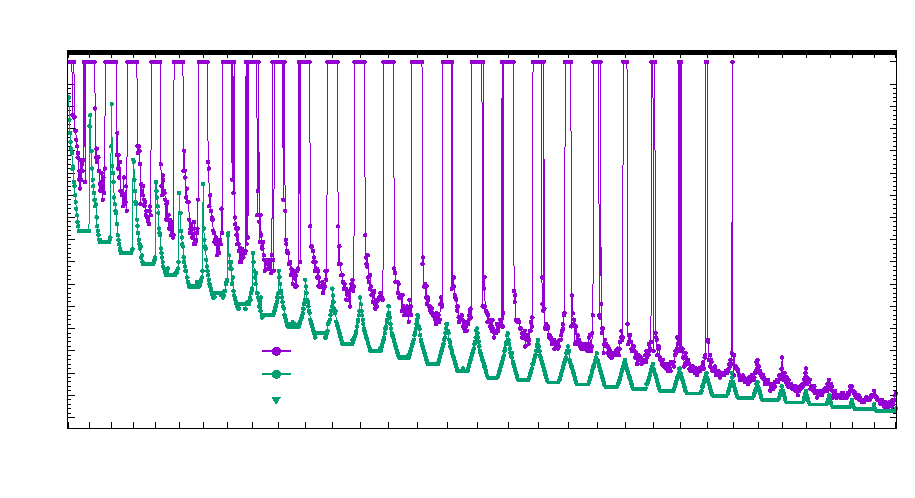
\includegraphics{resultados_8x8}}%
    \gplfronttext
  \end{picture}%
\endgroup
%
	\end{figure}
	}%
\end{frame}

\begin{frame}{Ejemplo ilustrativo en malla de $\mathsf{8\times 8}$}
	\captionsetup[figure]{belowskip = 0.5pt}%
	\vskip -7pt%
	\begin{figure}[H]
		\caption{Acomodo aleatorio inicial (izquierda) y acomodo encontrado por el algoritmo (derecha), mostrados en diferentes vistas.}%
		\arregloAntesDespues{caso=8x8, separacionAntesDespues=4.2, separacionVertical=0.26cm}{width=4.4cm}[width=4.348235cm]{width=2.9cm}%
	\end{figure}
\end{frame}

	
\begin{frame}{Tabla de resultados}
\vfill%
\setstretch{1.15}%
Resultados del algoritmo propuesto para mallas de tamaño igual o menor a 4\:$\times$\:4.
\fontsize{14}{14}\selectfont%
\begin{table}[H]
\renewcommand{\arraystretch}{1.4}%
\setlength{\arrayrulewidth}{0.75pt}%
\setlength{\tabcolsep}{0pt}%
\begin{minipage}{\textwidth}
\centering%
\begin{tabular}{
	>{\centering\bfseries}m{0.15\textwidth} 
	>{\centering}m{0.19\textwidth} 
	>{\centering}m{0.19\textwidth} 
	>{\centering}m{0.22\textwidth} 
	>{\centering}m{0.25\textwidth}
}
	\hline%
	\bfseries Malla & %
	\bfseries \#\,Total casos & %
	\bfseries \#\,Casos óptimos & %
	\bfseries \hspace*{-10pt}\%\,Óptimos & %
	\bfseries Promedio de acciones extra\mpfootnotemark \tabularnewline \hline
	3\:$\bm{\times}$\:3 & 32 & 30 & 93.75 \% & 0.09 \tabularnewline 
	3\:$\bm{\times}$\:5 & 85 & 70 & 82.35 \% & 0.33 \tabularnewline 
	4\:$\bm{\times}$\:4 & 88 & 88 & 100 \% & 0 \tabularnewline
	\hline%
\end{tabular}
\footnotetext{Promedio de acciones (o costo global $T$) extra por caso. Este valor se calcula mediante la expresión $( \sum T - \sum T_{\text{opt}} ) /\textsl{\#\,Total casos}$, donde $\sum T_{\text{opt}}$ es la suma de costos óptimos para todos los casos probados.}%
\end{minipage}
%\caption{Resultados del algoritmo propuesto para mallas de tamaño igual o menor a $4\times 4$.}%
\end{table}
\end{frame}


%\renewcommand{\numdiap}{}
{
\makeatletter
\setbeamertemplate{headline}[default]
\def\beamer@entrycode{\vspace{-9.75pt}}
\makeatother
\begin{frame}{Referencias}
	\vspace{-2pt}%
	\fontsize{11.1}{13}\selectfont%
	\bibliographystyle{apalike}	
	\bibliography{Bibliografia}
\end{frame}
}


\frame[noframenumbering,plain]{\centering \fontsize{40}{40}\selectfont{\textsc{Gracias}}}



%==============================================================================================================================		
\end{document}
%==============================================================================================================================
